\documentclass[12pt,a4paper,twoside,openany,titlepage,final]{book}

\usepackage[dvips]{geometry}
\geometry{textwidth=15cm,textheight=24cm,top=3.5cm}

\usepackage[small,sf]{caption}

\usepackage{sectsty}
\allsectionsfont{\sffamily\raggedright}

\usepackage{lmodern}
\usepackage[T1]{fontenc}
\usepackage{textcomp}

\usepackage{array}
\extrarowheight4pt

\usepackage{supertabular}

% \usepackage{floatflt}

\usepackage{graphicx}

\usepackage{amsmath}
\usepackage{amssymb}
\usepackage{bm}
\usepackage{framed}

\usepackage{multicol}
\premulticols0.0em

\usepackage{fancyhdr}

\pagestyle{fancy}

\bibliographystyle{plain}

\usepackage{makeidx}

\usepackage{color}
\usepackage{braket}
\usepackage{siunitx}

\usepackage{subfigure}
\usepackage{wrapfig}
\DeclareGraphicsExtensions{.png, .jpg, .pdf, .eps} 

\definecolor{link_color}{rgb}{0,0,1}
\definecolor{MARK_color}{rgb}{1,0,0}
\definecolor{filename_color}{rgb}{0.6,0.6,0.6}
% This usepackage command MUST BE LAST !!!
% More details on the hyperref package, including an extensive list of global package options
% can be found at http://www.tug.org/applications/hyperref/manual.html
\usepackage[backref           = page,
            colorlinks        = true,
            linkcolor         = link_color,
            menucolor         = link_color,
            citecolor         = link_color,
            urlcolor          = link_color,
            bookmarksnumbered = true,
            hyperindex        = true]{hyperref}
\hypersetup{pdfauthor  = {Volker Blum et al.},
            pdftitle   = {AIMS Manual},
            pdfsubject = {A users manual for the code package FHI-AIMS}}
% For handling underscores with hyperref
\usepackage{xstring}
\let\oldhypertarget\hypertarget
\renewcommand{\hypertarget}[2]{
  \StrSubstitute{#1}{\_}{_}[\tempa]
  \StrSubstitute{\tempa}{\$}{dummy}[\tempb]
  \oldhypertarget{\tempb}{#2}
}
\let\oldhyperlink\hyperlink
\renewcommand{\hyperlink}[2]{
  \StrSubstitute{#1}{\_}{_}[\tempa]
  \StrSubstitute{\tempa}{\$}{dummy}[\tempb]
  \oldhyperlink{\tempb}{#2}
}

%\pagestyle{headings}
%\pagenumbering{arabic}

\linespread{1.0}

\newcommand{\la}{$\langle$}
\newcommand{\ra}{$\rangle$}
\newcommand{\boldk}{\mbox{\boldmath$k$}}
\newcommand{\boldr}{\mbox{\boldmath$r$}}
\newcommand{\bolds}{\mbox{\boldmath$\sigma$}}
\newcommand{\boldp}{\mbox{\boldmath$p$}}
\newcommand{\boldR}{\mbox{\boldmath$R$}}
\newcommand{\boldE}{\mbox{\boldmath$E$}}
\newcommand{\boldF}{\mbox{\boldmath$F$}}
\newcommand{\boldG}{\mbox{\boldmath$G$}}
\newcommand{\erf}{\mathop{\mathrm{erf}}}
\newcommand{\erfc}{\mathop{\mathrm{erfc}}}
\DeclareMathOperator{\Tr}{Tr}
\newcommand{\bfr}{{\bf r}}
\newcommand{\bfrp}{{\bf r'}}
\newcommand{\bfk}{{\bf k}}
\newcommand{\bfq}{{\bf q}}
\newcommand{\bfR}{{\bf R}}
\newcommand{\bfRp}{{\bf R'}}
\newcommand{\bfRpp}{{\bf R''}}
\newcommand*{\Vect}[1]{{\ensuremath{\boldsymbol{\mathbf{#1}}}}}
\newcommand*{\Mat}[1]{{\ensuremath{\underline{\mathbf{#1}}}}}
\newcommand*{\D}{\mathrm{d}} % differential
\newcommand*{\Laplacian}{\mathop{}\!\mathbin\bigtriangleup}
\newcommand*{\Del}{\Vect{\nabla}}

\renewcommand{\floatpagefraction}{0.75}

% don't like something in the Manual? \MARK{} it and readers will definitely notice!
\newcommand{\MARK}[1]{\textbf{\color{MARK_color} #1}}

\newcommand{\keyword}[1]
{\hyperlink{#1}{\texttt{#1}}}

\newcommand{\subkeyword}[2]{\hyperlink{#1 #2}{\texttt{#2}}}

\newcommand{\option}[1]{\texttt{#1}}


% use this to define a keyword, automatically creates all the links here.
\newcommand{\keydefinition}[3]
{
\centerline{\rule{1.0\textwidth}{1pt}}
\hypertarget{#1}{\textbf{Tag: \texttt{#1}}{ \color{filename_color} (#2)}}
\index{#1@\texttt{#1}}
\\[2ex] \hspace*{0.05\textwidth}
\begin{minipage}{0.92\textwidth}
  #3
\end{minipage} \\
}

\newcommand{\subkeydefinition}[4]
{
\centerline{\rule{1.0\textwidth}{1pt}}
\hypertarget{#1 #2}{\textbf{\keyword{#1} sub-tag: \texttt{#2}} { \color{filename_color} (#3)}}
\index{#1@\texttt{#1}!#2@\texttt{#2}}
\\[2ex] \hspace*{0.05\textwidth}
\begin{minipage}{0.92\textwidth}
  #4
\end{minipage} \\
}

\newcommand{\keydefinitiontwo}[4]
{
\centerline{\rule{1.0\textwidth}{1pt}}
\hypertarget{#1}{\textbf{Tags:\ \texttt{#1}}{ \color{filename_color} (#3)}}
\hypertarget{#2}{\textbf{\newline\phantom{Tags:}\ \texttt{#2}\phantom{a}}{ \color{filename_color} (#3)}}
\index{#1@\texttt{#1}}
\index{#2@\texttt{#2}}
\\[2ex] \hspace*{0.05\textwidth}
\begin{minipage}{0.92\textwidth}
  #4
\end{minipage} \\
}

\newcommand{\keydefinitionthree}[5]
{
\centerline{\rule{1.0\textwidth}{1pt}}
\hypertarget{#1}{\textbf{Tags:\ \texttt{#1}}{ \color{filename_color} (#4)}}
\hypertarget{#2}{\textbf{\newline\phantom{Tags:}\ \texttt{#2}}{ \color{filename_color} (#4)}}
\hypertarget{#3}{\textbf{\newline\phantom{Tags:}\ \texttt{#3}}{ \color{filename_color} (#4)}}
\index{#1@\texttt{#1}}
\index{#2@\texttt{#2}}
\index{#3@\texttt{#3}}
\\[2ex] \hspace*{0.05\textwidth}
\begin{minipage}{0.92\textwidth}
  #5
\end{minipage} \\
}


\makeindex

\begin{document}

\fancyhf{}
\fancyhead[LO]{\sffamily\slshape \nouppercase{\rightmark}}
\fancyhead[RE]{\sffamily\slshape \nouppercase{\leftmark}}
\fancyhead[LE,RO]{\sffamily \thepage}
\fancypagestyle{plain}{
  \fancyhf{}
  \fancyhead[LE,RO]{\sffamily \thepage}
  \renewcommand{\headrulewidth}{0pt}
                      }
\renewcommand{\linespread}{1.0}

\parindent0.0ex
\parskip1.3ex

%\renewcommand{\baselinestretch}{1.0}

\sffamily

\thispagestyle{empty}
\vspace*{-2.0cm}

\begin{center} \huge
\centerline{\rule{1.0\textwidth}{1pt}}

\textbf{Fritz Haber Institute \\ \emph{ab initio} molecular
       simulations: FHI-aims}

\centerline{\rule{1.0\textwidth}{1pt}}

\vspace*{0.5cm}

\includegraphics[width=0.7\textwidth]{aims_logo}

\vspace*{0.5cm}

\LARGE {All-Electron Electronic Structure Theory \\ with Numeric Atom-Centered
  Basis Functions \\[3.0cm] A Users' Guide}
\end{center}

\vspace*{0.0cm}

\centerline{\rule{1.0\textwidth}{1pt}}
\begin{center} \large
     FHI-aims team
     \\
     with many contributors around the world. \\
\today
\end{center}

\newpage

\tableofcontents

\addcontentsline{toc}{chapter}{How to use this manual} 
\chapter*{How to use this manual}

If you are reading this introduction, you are likely reading the
manual for the first time. In that case, please read on. There is,
however, a strategy to use this manual most effectively to find
keywords used in the input files to FHI-aims. This is it:
\begin{itemize}
  \item Open the manual (pdf)
  \item Go to the table of contents
  \item At the bottom of the table of contents, click on ``Index''
  \item Find the keyword you are looking for in the index
  \item Click on it.
\end{itemize}
Using the manual in this way may greatly reduce the barrier to looking up
what a keyword actually does.

To first build FHI-aims, please also read this manual. You cannot simply type 'make'.
Chapter \ref{Ch:quickstart}, particularly sections \ref{Sec:installation}--\ref{Sec:build-cmake},
are what you need to read.

And now, for the actual ...

\chapter*{Introduction}
\addcontentsline{toc}{chapter}{Introduction} 

FHI-aims (``Fritz Haber Institute \emph{ab initio} molecular simulations'') is
a computer program package for computational materials science based only on
quantum-mechanical first principles. The main production method is density
functional theory (DFT) \cite{Hohenberg64,Kohn65,Dreizler90} to compute the total energy and
derived quantities of molecular or solid condensed matter in its electronic
ground state. In addition, FHI-aims allows to describe electronic
single-quasiparticle excitations in molecules using different self-energy
formalisms (e.g., $GW$ and MP2), and wave-function based molecular total energy
calculation based on Hartree-Fock and many-body perturbation theory (e.g., MP2,
RPA, SOSEX, or the more encompassing renormalized second-order
perturbation theory, RPT2). 

The basic physical algorithms in FHI-aims concerning ground state DFT and
applications are described in

\begin{center}
\parbox[c]{0.8\textwidth}
{\small
Volker Blum, Ralf Gehrke, Felix Hanke, Paula Havu, Ville Havu, Xinguo Ren,
Karsten Reuter, and Matthias Scheffler, Computer Physics Communications
\textbf{180}, 2175-2196 (2009). 
}
\end{center}

A copy of this paper can also be obtained from our web site: \\
\url{http://www.fhi-berlin.mpg.de/aims/} . \\ Please cite this reference if you use
FHI-aims. 

However, FHI-aims is not just a product of this basic reference.
Many more developments make this code a reality. For each individual
FHI-aims  run, a list of references describing the specific methods
used is given at the end of the FHI-aims standard output. Please give
credit in your publications if you can. FHI-aims is
a scientific code, written by and for scientists. The primary
recognition for their work is credit in the form of appropriate
reference to their work. 

Some particularly important papers (also worth reading!) follow
below. When making use of / reference to scalability, please refer to
and cite 

\begin{center}
\parbox[c]{0.8\textwidth}
{\small
Ville Havu, Volker Blum, Paula Havu, and Matthias Scheffler, Journal of
Computational Physics \textbf{228}, 8367-8379 (2009).
}
\end{center}

and also to the large-scale eigenvalue solver ELPA:

\begin{center}
\parbox[c]{0.8\textwidth}
{\small
A. Marek, V. Blum, R. Johanni, V. Havu, B. Lang, T. Auckenthaler, 
A. Heinecke, H.-J. Bungartz, and H. Lederer, 
The Journal of Physics: Condensed Matter \textbf{26}, 213201 (2014). 
}
\end{center}

Any application making use of functionality beyond LDA, GGA, or mGGA
-- i.e., Hartree-Fock, hybrid functionals, MP2, RPA, $GW$, etc. --
should please refer to and cite

\begin{center}
\parbox[c]{0.8\textwidth}
{\small
Xinguo Ren, Patrick Rinke, Volker Blum, J\"urgen Wieferink, Alex
Tkatchenko, Andrea Sanfilippo, Karsten Reuter, and Matthias Scheffler,
New Journal of Physics 14, 053020 (2012).
}
\end{center}

Further methodological publications for specific methods 
in FHI-aims can also be found at

\url{https://aimsclub.fhi-berlin.mpg.de/aims_publications.php}

Finally, we're quite proud that FHI-aims performed extremely well in the 
precision benchmark of 15 leading electronic structure codes known as
the ``Delta Project'', https://molmod.ugent.be/deltacodesdft -- see 
Reference \cite{Lejaeghereaad3000} in Science Magazine for
details.  
Numerical reliability -- high precision -- in everyday applications,
applicable up to very large production problems -- continues to be a top
priority and is, in fact, one of the key reasons why FHI-aims was
written in the first place. 

In the present documentation, we do not repeat the basic physical
algorithms; rather, the focus is on the actual \emph{use} of the methods in
FHI-aims for a given task, including a full description of all input and
output possibilities.  

The rest of this document is organized as follows:
\begin{itemize}
  \item In Chapter \ref{Ch:quickstart}, a ``quickstart'' 
    description attempts to give you all the necessary
    (but not more) information to get FHI-aims up and running on your own
    computer system, up to the first test run.
  \item Chapter \ref{Ch:basic} explains the basic input files and input
    philosophy very briefly. Some important remarks on choosing the numerical
    accuracy are summarized here.
  \item Chapter \ref{Ch:full} gets into the gory details, summarizing
    \emph{all} available input keywords and their meaning, sorted roughly by
    their expected use. 
  \item A large chapter \ref{CH:running} is dedicated to some frequently required
    ``meta-tasks'' of electronic structure theory: Not just setting up a
    specific set of input files for a given run, but actually extracting some
    of the frequently required information from those runs. For the more
    complex tasks (e.g., a transition state search), we attempt to provide
    scripts that perform a series of well-defined runs automatically, the 
    use of an external visualization tool, etc.  
  \item In chapter \ref{Ch:aitranss} we provide a description of the 
    \textsc{aitranss} ({\it ab initio} transport simulations) package which is
    a project under continuous development at the Institute of Nanotechnology  
    of the Karlsruhe Institute of Technology (KIT), Germany, since 2002. 
    When combined with FHI-aims, \textsc{aitranss} provides a
    post-processor module that enables calculation of the electron
    transport characteristics of molecular junctions based on a Landauer  
    formalism in a Green's function formulation.
  \item In the appendices, we suggest further reading, more on building
    the code from source, and we also address
    some issues (``troubleshooting'') that are either beyond
    our control (operating-system related issues come to mind), or simply
    require some level of experience to address.  
\end{itemize}
    Electronic structure
    theory (and FHI-aims) is extremely versatile but many of the most
    interesting applications require complex workflows. We cannot
    possibly document them all on our own. Please consider sending us
    hands-on descriptions of any complex workflows that worked for
    you, and we would gladly include them in this manual (obviously,
    we'll happily include references to your work).

In any case, we hope that this manual will be helpful for your specific
purposes. We welcome feedback, in particular regarding issues from
production settings that we might not yet have thought of / experienced
ourselves. In any event: Happy computing with FHI-aims! 



\chapter{Getting started with FHI-aims}
\label{Ch:quickstart}

\section{First step: Installation}
\label{Sec:installation}

FHI-aims comes as a gzipped tar archive that can be extracted in any directory
of your choice, e.g., by typing

\begin{verbatim}
  gzip -d fhi-aims.tar.gz
  tar -xvf fhi-aims.tar
\end{verbatim}

at the
command line of any current Unix-like system.

Note: You cannot simply type 'make'. To find out what to do for a
successful build, please look at sections
\ref{Sec:build-cmake}-\ref{Sec:cmake-variables}, which will tell you
what to do. There are a few performance related decisions that we
cannot make for you on an unknown computer system, and the description
below will hopefully help you make those decisions.

\begin{center}
  \parbox[c]{0.8\textwidth}
  {\small
    Before you ask: FHI-aims is designed to run on any current Unix-based or
    Unix-like system, such as Linux or Mac OS
    X. However, we do \emph{not} support FHI-aims on Windows at this point. It
    is certainly possible to make it run on a Windows platform using the
    appropriate tools, but not simply out-of-the-box. 
  } 
\end{center}

The full package then extracts itself into a directory \emph{./fhi-aims}, with the
following subdirectories:
\begin{itemize}
  \item \emph{bin/} : Location for any FHI-aims binaries built using the
    standard Makefile
  \item \emph{doc/} : Contains possible further documentation.
  \item \emph{species\_defaults/} : Grids, basis sets and other defaults for
    chemical elements 1-102. These can be copy-pasted as ``species'' into the
    FHI-aims input file \texttt{control.in}. FHI-aims provides three levels of
    standard species defaults: ``light'', ``tight'',
    and ``really\_tight'' (see Sec. \ref{Sec:species}). In addition,
    some further preconstructed special-purpose species defaults are
    provided in a ``non-standard'' subdirectory.
  \item \emph{src/} : This directory, and its subdirectories, contain all of FHI-aims source code files.
  \item \emph{testcases/} : Simple examples to test and illustrate the basic
    functioning of the code. The input files provided here may also be used as
    templates for any new electronic structure calculations, rather than
    assembling them from scratch.
  \item \emph{utilities/} : Some simple scripts to extract basic
    information from the standard output of FHI-aims:
    Visualization of geometries using the .xyz format, extracting a
    series of geometries during relaxation as a movie, or extracting
    the development of energies and forces during relaxation. There is
    also some more sophisticated infrastructure here: Script-based
    ab initio replica exchange molecular dynamics (Luca Ghiringhelli)
    and a basin-hopping framework to predict the structure of small
    clusters from scratch (Ralf Gehrke).
  \item \emph{regression\_tests/} : This directory contains a set of small standard
    test cases that can be run automatically using a script, \texttt{regressiontools.py} --
    when run without any flags, it will provide its own self-documentation.
    Unfortunately, running this script on a given platform and
    queueing system is not always trivial. If you can figure this out, we do recommend running and
    checking the regression tests on any new 
    machine on which FHI-aims was installed. We have encountered 
    rare but non-zero instances of compiler options (outside the
    control of FHI-aims) that produce correct numbers \emph{almost}
    always -- except for specific methods where the compiler has a
    bug. The regression tests will catch such issues before they
    strike in a production run. They 
    will allow to check the compiled FHI-aims binary a little more
    extensively, but they are not strictly necessary to run
    FHI-aims. In particular, please do \emph{not} view the input files
    of the regression tests as FHI-aims best practices. Follow the
    manual, not simply the regression tests. In many cases,
    they are not. Rather, what is tested may be a corner case that can
    be handled differently (better) in normal practical scenarios.
  \item \emph{benchmarks/} : This directory contains specific example
    runs of calculations, including output files and specific timings,
    illustrating how FHI-aims should perform and scale on a current
    high-performance computer. They also include some essential
    practices to get high performance and memory efficiency in
    FHI-aims for large runs on very large computers. We highly
    recommend trying to 
    run these benchmarks after successfully building FHI-aims on a
    parallel machine with sufficiently many CPUs. These benchmarks
    will give you an indication of whether you are achieving the
    expected performance of the code. This depends not only on
    building FHI-aims correctly, but also on the correct setup of the
    computing environment itself (not trivial). Running actual
    benchmarks is the best way to find out.
\end{itemize}
A \texttt{README} file in that directory contains some of the quickstart information
given here in condensed format. 

\section{Prerequisites (libraries and software) you'll need}
\label{Sec:prerequisites}

Since FHI-aims is distributed in source code form, the first task is to
compile an executable program. For this, the following \emph{mandatory
prerequisites} are needed:
\begin{itemize}
\item A working Fortran 2003 (or later) compiler. A good example for x86 type
  computers is Intel's \texttt{ifort} compiler.  A free but significantly slower
  compiler for all platforms is \texttt{gfortran} from the GNU compiler
  collection (\url{http://gcc.gnu.org/fortran}) or the \texttt{g95}
  compiler (\url{http://www.g95.org}). Do not underestimate this
  slowdown, though -- a factor of three or so is possible. 
  \item A compiled version of the \texttt{lapack} library, and a library
    providing optimized basic linear algebra subroutines (BLAS). Standard
    commercial libraries such as Intel's \texttt{mkl} or IBM's \texttt{essl}
    provide both \texttt{lapack} and BLAS support. \texttt{lapack} can also be found at
    \url{http://www.netlib.org/lapack/}. \\
    \emph{Having an optimized BLAS library for YOUR
    specific computer system(s) is critical for the performance of FHI-aims.}
    Very good free implementations include \texttt{ATLAS}
    (\url{http://math-atlas.sourceforge.net/}). 
\end{itemize}
You should also have a version of GNU Make and CMake for compiling FHI-aims. If CMake is not present, it is also possible to work with just GNU Make, but it is worth the effort to obtain CMake. Typically, GNU Make will already be present on your system, either as \texttt{make}, or possibly
as \texttt{gmake}. CMake should be available in the official repository of your Linux distribution.

The next two prerequisites are \emph{optional}, but absolutely
essential for any current use of FHI-aims: Support for parallel
architectures, and (separately) support for fully parallel
linear algebra. Thus, you will also
need: 
\begin{itemize}
  \item A version of MPI libraries for parallel execution, often already
    present on a parallel system (if not,
    \url{http://www.open-mpi.org/} provides one of several free
    implementations). Our experience is that Intel's MPI library is
    a very worthwhile investment on x86 platforms (better performance).
  \item Compiled versions of the \texttt{scalapack} library, and
     basic linear algebra \emph{communication} subroutines (BLACS). Capable
     implementations can be found at \url{http://www.netlib.org/}, but
     are often provided already in the numerical libraries of many
     vendors (e.g., Intel MKL on Linux).
\end{itemize}
Finally, the default compilation builds an executable which includes
some parts of the code that are written in C. This may be turned off (see
below), but we highly recommend compiling with C support as it introduces a
number of useful features.  You need:
\begin{itemize}
  \item A C compiler -- available on every Unix platform. The C parts
    are not performance critical and if you can, just use the GNU
    project's gcc compiler. gcc is compatible with many Fortran
    compilers, most importantly also Intel Fortran, and our experience
    is that gcc presents fewer problems than other (commercial) C
    compilers. 
\end{itemize}
  
\textbf{The creation of a complete, MPI-, scalapack-, and C-enabled binary
  is effort well spent. This should be the goal when compiling FHI-aims
  for any production purposes. This means that you should ultimately
  aim to build FHI-aims with the \texttt{USE\_MPI} and \texttt{USE\_SCALAPACK} CMake options enabled (see below).}

To create an actually working FHI-aims build, please read sections~\ref{sec:minimal_cmake}--\ref{sec:CMake_variables}. Beyond that, the ``aimsclub'' Wiki gives
compilation hints for many platforms (including MPI, BLACS and
Scalapack, which we strongly recommend on any platform with more than
one CPU). Please help by adding your own working settings there, and
ask us if there are questions. For the many other ways of how to reach
us, please see Section \ref{Sec:community} below.

\section{Managing the build process with CMake}
\label{Sec:build-cmake}

Building of FHI-aims is managed by CMake, which is a free and open-source build system generator. A build system generator is a tool that does not build anything by itself. Instead, it generates build scripts for a particular build system, e.g., Make, which are then used for the actual building. The build scripts, e.g., makefiles, are generated based on the user's environment and it is the job of CMake to ensure that the generation stage is as straightforward and failsafe as possible. In principle, CMake is completely platform agnostic (the C stands for cross-platform), but currently the focus is on supporting FHI-aims in a Linux environment only.

CMake was released in 2000 and is currently used in a large number of projects (including some big ones like HDF5, KDE, mySQL, and Netflix). One of the motivators for FHI-aims was a push from the ESL (Electronic Structure Library) project to adopt CMake as the build management standard. ESL is a collection of electronic structure codes with the aim of avoiding duplication of functionality by connecting different electronic structure codes with each other with minimal effort. That is one of the reasons to use CMake as it makes it relatively easy to include other CMake projects into a given project.

\subsection{\label{sec:minimal_cmake}Example CMake usage}

Here is a typical example to get you started with CMake.
\begin{enumerate}
\item Go to the root directory of FHI-aims and create a build directory:
\begin{verbatim}
mkdir build && cd build
\end{verbatim}
\item Create a file called \texttt{initial\_cache.cmake} in the build directory or make a copy of \texttt{initial\_cache.example.cmake} which is in the root directory. The following is example contents for that file,
\begin{verbatim}
set(CMAKE_Fortran_COMPILER "mpif90" CACHE STRING "")
set(CMAKE_Fortran_FLAGS "-O3 -ip -fp-model precise" CACHE STRING "")
set(CMAKE_C_COMPILER "icc" CACHE STRING "")
set(CMAKE_C_FLAGS "-O3 -ip -fp-model precise" CACHE STRING "")
set(LIB_PATHS "/opt/intel/mkl/lib/intel64" CACHE STRING "")
set(LIBS "mkl_intel_lp64 mkl_sequential mkl_core
mkl_blacs_intelmpi_lp64 mkl_scalapack_lp64" CACHE STRING "")
set(USE_MPI ON CACHE BOOL "")
set(USE_SCALAPACK ON CACHE BOOL "")
set(USE_HDF5 OFF CACHE BOOL "")
\end{verbatim}
  which you can edit to reflect your environment.
\item Issue
\begin{verbatim}
cmake -C initial_cache.cmake ..
\end{verbatim}
  from the build directory to configure.  If you encounter any errors during this step, we recommend correcting your \texttt{initial\_cache.cmake} file, saving it, then deleting the build directory and restarting from the first step.
\item Issue
\begin{verbatim}
make -j
\end{verbatim}
to build. An executable whose name starts with \texttt{aims} is created in the same directory.
\end{enumerate}
For more details on how to use CMake, see Sec.~\ref{Sec:cmake}.

\section{CMake variables}
\label{Sec:cmake-variables}

Here are some of the commonly used CMake variables.

\begin{itemize}
\item \texttt{CMAKE\_Fortran\_COMPILER} --- Name of the Fortran compiler executable. Use a full path if location not automatically detected.
\item \texttt{CMAKE\_Fortran\_FLAGS} ---  Compilation flags that control the optimization level and other features that the compiler will use. \item \texttt{LIB\_PATHS} --- List of directories to search in when linking against external libraries (e.g., ``/opt/intel/mkl/lib/intel64'')
\item \texttt{LIBS} --- List of libraries to link against \\
  (e.g., ``mkl\_blacs\_intelmpi\_lp64 mkl\_scalapack\_lp64'')
\item \texttt{USE\_MPI} ---  Whether to use MPI parallelization when building FHI-aims. This should always be enabled except for rare debugging purposes. (Default: automatically determined by the compiler)
\item \texttt{USE\_SCALAPACK} --- Whether to use Scalapack's parallel linear algebra subroutines and the basic linear algebra communications (BLACS) subroutines. It is recommended to always use this option. In particular, large production runs are not possible without it. The Scalapack libraries themselves should be set in \texttt{LIB\_PATHS} and \texttt{LIBS}. (Default: automatically determined by \texttt{LIBS})
\item \texttt{USE\_C\_FILES} ---  Whether source files written in C should be compiled into FHI-aims.  By default, this is \texttt{ON}, i.e. C files will be compiled.  These routines are not performance-critical but can access environment variables. They can thus provide useful additional output about the computer system environment used and also make a few other useful libraries accessible (like Spglib for symmetry handling). If not enabled, appropriate stub files are compiled instead.
\item \texttt{CMAKE\_C\_COMPILER} --- C compiler. Usually gcc is fine here.
\item \texttt{CMAKE\_C\_FLAGS} --- C compiler flags.
\item \texttt{USE\_LIBXC} --- Whether additional subroutines for exchange correlation functionals, provided in the LibXC library, should be used. By default, this is \texttt{ON}, i.e. LibXC will be compiled into the executable.  It is advised to always use this. Please respect the open-source license of this tool and cite the authors if you use it.
\item \texttt{USE\_SPGLIB} ---  Whether the Spglib library for symmetry handling will be used.  By deafult, this is \texttt{ON}, i.e. Spglib will be compiled into the executable.  Please respect the open-source license of this tool and cite the authors if you use it.
\end{itemize}

For all CMake variables, see Sec.~\ref{sec:CMake_variables}.

\subsection{MPI parallelization}

In order to force MPI to be disabled, put
\begin{verbatim}
set(USE_MPI OFF CACHE BOOL "")
\end{verbatim}
into the initial cache file. In order to force MPI to be enabled, use
\begin{verbatim}
set(USE_MPI ON CACHE BOOL "")
\end{verbatim}
instead. If you want to enable/disable MPI support after the first configuration, issue
\begin{verbatim}
ccmake ~build
\end{verbatim}
where $\sim$\texttt{build} is the build directory. Move cursor to the field \verb+USE_MPI+ and hit enter. This toggles its state between \texttt{ON/OFF}. Hit 'c' to configure, 'g' to generate the build files, and rebuild the project.

\section{Running FHI-aims}
\label{Sec:running}

As a simple test run to establish the correct functioning of FHI-aims and also
to familiarize yourself with the basic structure of the input and output
files, we suggest you change directories to the
\emph{testcases/H2O-relaxation/} directory. The test run provided there relaxes
a simple H$_2$O molecule from an initial (distorted) structure to the stable
one, and computes total energies, eigenvalues etc. along the way. Notice that
the key convergence settings (basis sets and grids) in this example are chosen
to be fast. The results (particularly the relaxed geometry) are still
trustworthy, but we encourage you already here to explore more
stringent convergence settings later. In fact, \emph{always} explore the
impact of critical convergence settings on the accuracy of key results in your
own project.

In the \emph{testcases/H2O-relaxation/} directory, type

{
  \verb+ ../../src/aims.+\emph{version}\verb+ < /dev/null | tee H2O_test.own+
}

at the command line. For ``\emph{version}'', you must insert the code version stamp 
that was actually downloaded and built (for example, \verb+171221+ or
whichever code version you are building).\footnote{The  
FHI-aims version stamp can be modified to whatever you wish in
\texttt{Makefile.backend} in the \emph{src/} directory.} 
For faster execution, you should use the appropriate binary including the necessary mpi command
instead. On many (but not all) platforms, that command will be
\texttt{mpirun}, and will also require you to specify the number of processors
to be used by a flag. For 20
CPU cores, this could look like

{
  \verb+ mpirun -np 20 ../../src/aims.+\emph{version}\verb+ < /dev/null | tee H2O_test.own+
}

The result will be an output stream on your computer screen (created by
``tee'') which is also captured in an output file \texttt{H2O\_test.own}. 
Any critical information regarding computational
settings, results (total energies, forces, geometries, ...), errors
etc. should be contained in this file, which we encourage you to look at (yes,
it is \emph{meant} to contain human-readable and useful explanations). Any \emph{other} output files are  
only written if requested, and will be covered in the later sections of this
text.

\begin{center}
  \parbox[c]{0.8\textwidth}
  {
  \emph{The standard output stream or file contains any and all output that FHI-aims
  writes by default. For later use, you must save this output stream to disk in some way, 
  using standard Unix redirections such as the \texttt{tee} command above or a simple 
  redirect.}
  }
\end{center}

  Apart from the first expression given above, such 
  redirections might look like this: 

  {
    \verb+ mpirun ../../bin/aims.+\emph{version}\verb+.scalapack.mpi.x < /dev/null > H2O_test.own+
  }

  or even like this: 

  {
    \verb+ nohup mpirun ../../src/aims.+\emph{version}\verb+ < /dev/null > H2O_test.own 2>&1 &+
  }

  The latter version decouples the FHI-aims run completely from your
  current login shell and additionally
  saves any system error messages to the standard output file as well. With the above command sequence,
  you may safely log out from the computer in question, the code should keep running in the background. 

  Take care to monitor your running processes using the \texttt{ps} Unix command. For instance, it is
  highly unadvisable to run ten instances of FHI-aims at once in the background on a single CPU and expect
  any reasonable performance of the computer at all. The above hints
  are just examples of general Unix command-line sequences. For a complete treatment, we
  recommend that beginners read a separate Unix textbook, or---often feasible---learn by doing and Google. 

If successful (otherwise, consider the warnings three paragraphs below), you
may wish to compare your results to those contained in our 
own output from this run, which is contained in the file
\texttt{H2O.reference.out}. You should obtain exactly the same total energies,
forces, and geometries as given in this file. Any information regarding timing
is, of course, specific to your computer environment, and not necessarily the
same. 

The directory \emph{testcases/H2O-relaxation/} contains two more files,
\texttt{control.in} and \linebreak[4] \texttt{geometry.in}. These are the sole two input
files required by FHI-aims, and are the most important files to learn about in
the rest of this documentation. In brief, \texttt{geometry.in} contains any
information related directly to a system's geometry -- normally, this will be
atomic positions (in \AA) and perhaps lattice vectors for periodic
calculations, but no more. Any other, method-related, input information is
part of \texttt{control.in}. 

In practice, we attempt to strike a balance
between the information \emph{needed} by \linebreak[4] \texttt{control.in}, and information
set to safe defaults unless specified explicitly. For example, you \emph{must}
specify the level of theory (e.g., the fact that PBE exchange-correlation is
used) and also the basis set and other numerical settings employed. While it is highly useful to
have this relevant information openly accessible, this  
would also create the need to personally edit a large amount of input before ever
tackling the first run. For any information tied to the actual element (or
``species''; arguably the most complex information required), we therefore provide
ready-made template files for all elements (1-102) in the
\emph{species\_defaults} directory. They are ready for copy-paste into
\texttt{control.in}. These files will still benefit from some
adjustment to your personal needs (for instance, the provided integration
grids are set rather on the safe side, at the expense of more CPU time), but
should greatly simplify the task. 

Two final, important warnings regarding the execution of FHI-aims that are beyond
our direct control:
\begin{itemize}
  \item FHI-aims \emph{requires} that the execution stack size available to
    you be large enough for some initial internal operations. Spare us the
    details (ample explanation of the meaning of the ``stack'' in Unix can be
    found elsewhere), but for reasons unbeknownst to us, some vendors limit
    the default user stack size to $\approx$5~MB at a time when the typical
    available system memory per processor is 2 GB or more. If too little stack is
    available, your FHI-aims run will \emph{segfault} shortly after the
    command was launched. To avoid this, \texttt{always} type:
    \begin{verbatim}
        ulimit -s unlimited
    \end{verbatim}
    (when using the bash shell or similar), or
    \begin{verbatim}
        limit stacksize unlimited
    \end{verbatim}
    (when using the tcsh or similar). 
    \begin{verbatim}
        echo $SHELL
    \end{verbatim}
    will tell you which shell you are using. Ideally, this same setting should
    be specified in your .profile, .bashrc, or .cshrc login profiles. If
    ``unlimited'' is prohibited by your computer (e.g., on MacOS), try
    setting a large value instead, e.g.,
    \texttt{ulimit -s 500000}.
  \item An important system settings for parallel execution is the environment
    variable  
    \begin{verbatim}
      export OMP_NUM_THREADS=1
    \end{verbatim}
    (the syntax is correct for the bash shell). When using Intel's mkl, you
    should additionally set \texttt{MKL\_NUM\_THREADS} to 1 and
    \texttt{MKL\_DYNAMIC} to FALSE.
  \item Do not try to use OpenMP with FHI-aims unless you know exactly
    why you are doing this. FHI-aims is very efficiently
    MPI-parallelized and large portions of the code do not support
    OpenMP at all. (And they do not need to -- MPI is simple as effective
    or more effective on practically all platforms in our experience.)
\end{itemize}

After startup, the first messages contain information about your computer's 
environment: Code version, compiler information, host names, environment 
variables which turned out to be useful and which should be set on
your system (e.g.~\texttt{OMP\_NUM\_THREADS}), etc. The complete input
files \texttt{control.in} and \texttt{geometry.in} are also repeated
verbatim. Any FHI-aims run should thus be completely reproducible
based on the standard output stream alone.

Should you encounter further issues, consider also the troubleshooting
information documented in Appendix \ref{appendix_trouble_shooting}. 

All this said, after successfully running the test run, you should now be
ready to go with FHI-aims. The remainder of this document is about the details
-- available options, how to run aims most efficiently, etc. Happy computing!


\section{Compiling faster versions of FHI-aims on specific platforms}
\label{Sec:Platform}

FHI-aims is intended to be a Fortran-only code, which -- for most of
the code -- means that building the ``fastest'' version of FHI-aims on
a given computer architecture is ``only'' a matter of finding the
right Fortran compiler and compiler options for that processor. For
some architectures, specific compiler options are collected in the
FHI-aims club wiki -- please check there and please add any useful
information that you may find.

That said, one particular performance-critical area for large systems
is the Kohn-Sham eigenvalue solver. In FHI-aims and on parallel
computers, this problem is solved by the ELSI infrastructure and the
ELPA library. ELPA, in fact, 
allows its users to specify specific, platform-optimized so-called
linear algebra ``kernels.'' By default, FHI-aims uses a generic kernel
which will compile with any Fortran compiler and will give reasonable
speed. However, if one knows which specific computer chip one is
using, it is possible to substitute this kernel with an architecture
specific kernel and compile a faster version of ELPA into
FHI-aims. This is possible, for example, for the BlueGene/P,
BlueGene/Q, Intel AVX and several other Intel architectures. For
standard Intel x86 chips, there is even an ``assembler'' based kernel
that will get fast performance regardless of the Fortran compiler
above.

Note that this choice can matter. For example, the ``generic'' ELPA
kernel will produce fast code for the Intel Fortran compiler, but much
slower code with certain versions of the PGI Fortran compiler (often
found on Cray machines).

At this time, please ask (see below) about the most effective strategy
to link against the ``best'' ELSI and ELPA libraries. Ideally, this
will require a user to build a separate (standalone) instance of ELPA
and of ELSI first. This can be very worthwhile.

\section{Finding the other FHI-aims developers and users (talk to us!)}
\label{Sec:community}

It can be surprisingly useful (and more fun) to find others who work with
FHI-aims -- to help find out who might already have solved a specific
problem, how a given problem might be solved, exchange experiences,
devise new and cool functionality that could take electronic structure
theory to the next level, and so on. Some of us also simply like to have
a cup of coffee with others (see below). FHI-aims only functions as a code and
science tool because of the community around it, and we're always
happy to meet new users, developers, and generally find out how to do
better science together.

At the time of writing, we have a number of active communication
channels. Anyone using or developing with FHI-aims is encouraged
to frequent one or all of them:
\begin{itemize}
  \item The forums and wiki at \textit{aimsclub},
    \url{https://aimsclub.fhi-berlin.mpg.de/} . This is a place where
    questions can be asked, answered, and looked up, and anyone is
    welcome and encouraged to share their experiences
    there. Additionally, wiki entries are also encouraged. If nothing
    else, the wiki is a place to let the rest of the world know of
    successful build settings for FHI-aims on different platforms.
  \item An active \textit{slack channel} (chat) at
    \url{https://fhi-aims.slack.com/} . This is a place where a number of
    developers and users hang out and can 
    be easily reached for questions in public semi-private and private
    conversations. Pretty effective. To join, you'll need an invitation from one of the
    slack channel owners, which we'll happily provide. Just ask, for
    example via aimsclub or by email (volker.blum@duke.edu is one
    of the owners, and there are several others as well).
  \item \textit{Monthly FHI-aims video meetings} for anyone with an
    interest, usually announced on aimsclub and on the slack channel. 
  \item \textit{FHI-aims Users' and Developers' meetings}, which we hold
    roughly every two years.
  \item For those who use the FHI-aims mainline (development)
    version -- everyone with an FHI-aims license is welcome and
    encouraged to ask for access to this usually very stable version
    -- there is a \textit{``buildbot''} that shows the current status
    of FHI-aims' regression tests for a variety of platforms,
    compilers, and other choices at any given time. The buildbot can
    be accessed at \url{http://www.theo.ch.tum.de/bbot/\#/} .
  \item Finally, for those who are shy, you are also welcome to \textit{email}
    us: \\
    At aims-coordinators@fhi-berlin.mpg.de or (for those who are
    even more shy) email Volker, the lead developer, at
    volker.blum@duke.edu . Email is a productive avenue and Volker
    answers to the best of his abilities and available human time. However,
    bear in mind that one of the above channels will also reach Volker
    and, in addition, the many others who make FHI-aims happen and who
    might already have solved a  problem and have an answer
    ... although you'd never have thought anyone did. 
\end{itemize}
In short -- please feel welcome and encouraged to talk to us if
useful. FHI-aims is about science, and we're accessible. And if you're
new to all this and someone helped you out especially, feel free to send
them a Starbucks gift card (no one has ever done that, but hey, you
could be the first :) or, even
better, to cite their contribution to FHI-aims. 


\chapter{Input Files: Basic Handling}
\label{Ch:basic}

\section{The mandatory input files: \texttt{control.in} and \texttt{geometry.in}}

As discussed in Sec. \ref{Sec:running}, FHI-aims requires exactly two input
files---\texttt{control.in} and \texttt{geometry.in}---located in
the same directory from which the FHI-aims binary is invoked. To start
FHI-aims, no further input should be needed.\footnote{A few specific keywords
  (e.g., a restart of an existing calculation from an earlier wave function
  or density matrix) may require
  additional input that simply can not be included in user-edited file. Such
  input files will be described with the appropriate tasks.}

\begin{figure}
  \small
  \begin{verbatim}
# Geometry for water -- needs to be relaxed as the water molecule 
# described here has a 90degree bond angle and a 
# 1 Angstrom bond distance ... 
atom    0.00000000    0.00000000    0.00000000    O
atom    0.70700000   -0.70700000    0.00000000    H 
atom   -0.70700000   -0.70700000    0.00000000    H 
  \end{verbatim}
  \normalsize
  \caption{\label{Fig:geometry.in}
    Example input file \texttt{geometry.in}, provided with the simple
    test case (relaxation of H$_2$O) described in Sec. \ref{Sec:running}.
  }
\end{figure}

\begin{figure}
  \small
  \begin{verbatim}
#########################################################################################
#
#  Volker Blum, 2017 : Test run input file control.in for simple H2O
#
#########################################################################################
#
#  Physical model
#
  xc                 pbe
  spin               none
  relativistic       none
  charge             0.
#
#  Relaxation
#
  relax_geometry   bfgs 1.e-2
#
################################################################################
#
#  FHI-aims code project
#  VB, Fritz-Haber Institut, 2009
#
#  Suggested "light" defaults for H atom (to be pasted into control.in file)
#  Be sure to double-check any results obtained with these settings for post-processing,
#  e.g., with the "tight" defaults and larger basis sets.
#
################################################################################
  species        H
#     global species definitions
    nucleus             1
    mass                1.00794

[...]

  \end{verbatim}
  \normalsize

  \vspace*{-4.0ex}

  \caption{\label{Fig:control.in}
    Excerpts from the example input file \texttt{control.in}, provided with the simple
    test case (relaxation of H$_2$O) described in Sec. \ref{Sec:running}. A
    section of \emph{general} (system-wide) run-time settings is separate from
    individual sections that describe settings specific to certain
    \emph{species} (chemical elements).
  }
\end{figure}

Figures \ref{Fig:geometry.in} and \ref{Fig:control.in} show as examples the
\texttt{geometry.in} and \texttt{control.in} files used for the simple test
case (relaxation of a water molecule) described in Sec. \ref{Sec:running}. The
philosophy of their separation is simple:
\begin{itemize}
  \item \texttt{geometry.in} contains only information directly related to the
    atomic structure for a given calculation. This obviously includes atomic
    positions, with a description of the particulars of each element (or
    \emph{species}) expected in \texttt{control.in}. In addition, lattice
    vectors may be defined if a periodic calculation is required. Any other
    information is only given here if it is \emph{directly} tied to the atom
    in question, such as an initial charge, initial spin moment, relaxation
    constraint etc. The order of lines is irrelevant, except that information
    specific to a given atom must follow \emph{after} the line specifying that
    atom, and \emph{before} any following atom is specified.
  \item \texttt{control.in} contains all other runtime-specific
    information. Typically, this file consists of a \emph{general} part,
    where, again, the particular order of lines is unimportant. In addition,
    this file contains \emph{species} subtags that are references by
    \texttt{geometry.in}. Within the description of a given species, the order
    of lines is again unimportant, but \emph{all} information concerning the
    same species must follow the initial \emph{species} tag in one block.
\end{itemize}
In both files, the choice of units is {\AA} for length parameters, and eV for
energies; derived quantities are handled accordingly. Lines beginning with a \#
symbol are treated as comments, and empty lines are ignored. Finally, each
non-comment line has the following, free-format structure:

\begin{verbatim}
  keyword value <value> <value>
\end{verbatim}

Generally, all keywords and values are case sensitive: Do not expect FHI-aims
to understand an ``XC'' keyword if the specified syntax is ``xc''. 

It is the objective of the \emph{next} chapter, Chapter \ref{Ch:full},
to list all legitimate keywords in FHI-aims, and to describe their
function. 


\section{Defaults for chemical elements: species\_defaults}
\label{Sec:species}

FHI-aims requires exactly two input files, located in the same directory where
a calculation is started: \texttt{control.in} and \texttt{geometry.in}. Both
files can
in principle be specified from scratch for every new calculation, using the
keywords listed in Chapter \ref{Ch:full}. However, choosing the central
computational settings consistently for series of calculations greatly
enhances the accuracy of any resulting energy differences (error cancellation).

In FHI-aims, the key parameters regarding computational accuracy are actually
subkeywords of the \keyword{species} keyword of \texttt{control.in},
controlling the basis set, all integration grids, and the accuracy of the
Hartree potential. These settings should of course not be retyped from scratch
for every single calculation; on the other hand, they should remain obvious
to the user, since these are the central handles to determine the accuracy and
efficiency of a given calculation. 

FHI-aims therefore provides preconstructed default definitions for the
important subkeywords associated with different \keyword{species} (chemical
elements) from $Z$=1-102 (H-Md). These can be found in the
\emph{species\_defaults} subdirectory of the distribution, and are built for
inclusion into a \texttt{control.in} file by simple copy-paste. 

For all elements, FHI-aims offers three or four different levels of
\emph{species\_defaults}: 
\begin{itemize}
  \item \emph{light} :
    Out-of-the-box settings for fast prerelaxations, structure searches,
    etc. In our own work, no obvious geometry / convergence errors resulted
    from these settings, and we now recommend them for many household
    tasks. For ``final'' results (meV-level converged energy differences between
    large molecular structures etc), any results from the \emph{light} level
    should be verified with more accurate post-processing calculations,
    e.g. \emph{tight}. 
  \item \emph{intermediate} :
    This level is presently only available for a few elements, but can
    play an important role for large and expensive calculations,
    especially for hybrid functionals. \emph{Intermediate} settings
    use most of the  
    numerical settings from \emph{tight}, but includes basis functions
    between \emph{light} and \emph{tight}. The cost of hybrid
    functionals scales heavily with the number of basis functions
    found on a given atom. Full \emph{tight} settings, which were
    designed with the much cheaper semilocal functionals in mind, can
    be prohibitively expensive for large structures and hybrid density
    functionals. Hybrid DFT results from \emph{intermediate} settings
    are typically completely sufficient for production results, much
    cheaper, and we hope to produce \emph{intermediate} defaults for a
    wider range of elements in coming years.
  \item \emph{tight} : 
    Regarding the integration grids, Hartree
    potential, and basis cutoff potentials, the settings specified here are
    rather safe, intended to provide meV-level accurate energy
    \emph{differences} also for large structures. In the \emph{tight} settings,
    the basis set level is set to \emph{tier} 2 for the light elements 1-10, a
    modified \emph{tier} 1 for the slightly heavier Al, Si, P, S, Cl (the first
    \emph{spdfgd} radial functions are enabled by default),
    and \emph{tier} 1 for all other elements. This reflects the fact that, for
    heavy elements, \emph{tier} 1 is sufficient for tightly converged ground
    state properties in DFT-LDA/GGA, but for the light elements (H-Ne),
    \emph{tier} 2 is, e.g., required for meV-level converged energy
    differences. For convergence
    purposes, the specification of the basis set itself (\emph{tier}
    1, \emph{tier} 2, etc.) may still be 
    decreased / increased as needed. Note that especially for hybrid functionals,
    \emph{tight} can already be very expensive and specific reductions
    of the number of radial functions may still provide essentially
    converged results at a much more affordable cost (see
    \emph{intermediate} settings).
  \item \emph{really\_tight} : 
    Same basis sets (radial functions and cutoff radii) as in the
    \emph{tight} settings, but for the other numerical aspects (grids,
    Hartree potential), settings that are \emph{strongly
    overconverged} settings for most purposes. The idea is that
    \emph{really\_tight} can be used for very specific, manual
    convergence tests of the basis set and other settings -- if really
    needed. \\ 
    Note that the \emph{``tight''} settings are intended to
    provide reliably accurate results for most DFT production
    purposes; and they are not cheap. The absolute total energies for
    \emph{tight} and DFT are in practice converged to some tens of
    meV/atom for most elements. To go beyond, take the
    \emph{really\_tight} settings and increase the basis set or other
    numerical aspects step by step. (Radial function by radial 
    function may often be a good strategy to go.) \emph{We emphasize
    that the \emph{really\_tight} settings should only ever be
    needed for individual, specific tests. They should not be
    needed for any standard production tasks unless you have
    seriously too much CPU time to spend.} \\ Specific differences
    between \emph{tight} 
    and the unmodified \emph{really\_tight} settings: The
    \subkeyword{species}{basis\_dep\_cutoff} keyword is set to zero, a
    prerequisite to approach the converged basis limit. Regarding the
    Hartree potential, \subkeyword{species}{l\_hartree} is set to 8,
    and the maximum number of angular grid points per radial
    integration shell is increased to 590. \\  
    Note that there can still
    be corner cases where you may want to test some numerical setting
    beyond \emph{really\_tight}. Mostly, these are custom scenarios or
    things beyond standard FHI-aims calculations of DFT total
    energies. Examples include: The confinement radius for surface
    work functions (should be checked), use of very extended or
    extremely tight Gaussian-type orbital basis functions (e.g., from
    very large Dunning-type basis sets -- the density of the radial
    and angular grids should be checked), or RPA and MP2 calculations,
    which can need very different and often much larger basis sets
    (again, radial and angular grids should be checked). 
\end{itemize}

A separate group of species defaults for light elements (H-Ar) is
available especially for calculations involving explictly correlated
methods (methods other than semilocal and hybrid density functionals): 
\begin{itemize}
  \item \emph{NAO-VCC-nZ} : NAO type basis sets for H-Ar by Igor Ying
    Zhang and coworkers \cite{Zhang2013}. These basis sets
    are constructed according to Dunning's ``correlation consistent''
    recipe. Their intended application is for methods that invoke
    the continuum of unoccupied orbitals explicitly, for instance MP2,
    RPA or $GW$. Note that they were constructed for valence-only
    correlation (hence ``VCC'', valence correlation consistent), i.e.,
    they work best in frozen-core correlated approaches following a
    full s.c.f. cycle (core and valence) to generate the
    orbitals. While NAO-VCC-nZ can be used for ``normal'' density
    functional theory (LDA, GGA, or hybrid functionals), the normal
    ``light'', ``intermediate'', ``tight'' and ``really\_tight'' species defaults are
    more effective in those cases. The advantage of NAO-VCC-nZ over
    GTO basis sets such as the Dunning ``cc'' basis sets is that with
    NAOs, both the behaviour near the nucleus as well as that for the
    tails of orbitals far away from atoms is much more physical. This
    means that we can use more efficient integration grids than for
    GTO basis sets to obtain systematic convergence of the unoccupied
    state space. 
\end{itemize}

The \textit{NAO-J-n} basis sets are designed for the calculation of indirect spin-spin coupling constants (J-couplings):
\begin{itemize}
\item \textit{NAO-J-n} : The basis sets are available for most light elements from H to Cl. Since these are more expensive (tighter grids) than other basis sets, they should only be used for J-couplings. Even then, they should only be placed on atoms of interest, while cheaper basis sets can be used on other atoms. They are constructed by adding tight Gaussian orbitals to the NAO-VCC-nZ basis sets. In order to describe the Gaussian orbitals correctly near the nucleus, tighter grids than normally are required (with \keyword{radial\_multiplier} 8 and \keyword{l\_hartree} 8, among other parameters). Other stages of the calculation, such as geometry relaxation, should be performed with basis sets more suitable for the particular task (using, e.g., the default tight settings).
\end{itemize}

In addition, the \emph{species\_defaults} directory contains a few
more sets of species defaults for special purposes. These can be found
in the \emph{non-standard} subdirectory and include:
\begin{itemize}
  \item \emph{gaussian\_tight\_770} : Species defaults that allow to
    perform calculation with some standard published Gaussian-type
    orbital (GTO) basis sets for elements H-Ar (including basis sets due to
    Pople, Dunning, Ahlrichs and their coworkers). These species
    defaults are meant to allow for exact benchmarks against
    GTO codes such as NWChem. The other
    numerical settings (especially grids) are thus much tighter than
    needed for ``normal'' NAO-type calculations. Note that FHI-aims is
    not optimized for GTO basis sets. We recommend
    NAO-type basis sets, not GTO basis sets, for production
    calculations -- NAO-type basis sets are much easier to handle
    with our techniques and give better accuracy at lower cost. That
    said -- the grid settings in the \emph{gaussian\_tight\_770}
    species defaults are rather overconverged for benchmark
    purposes. One could create much more efficient species defaults for
    GTO basis sets -- but GTOs still would not be as efficient as NAO
    basis sets (at the same level of accuracy).
  \item \emph{Tier2\_aug2} : Example, pioneered by Jan Kloppenburg, of
    basis sets that merge FHI-aims' tier2 basis sets with a very
    reduced set of Gaussian augmentation functions taken from
    Dunning's augmented correlation-consistent basis sets. This
    prescription appears to provide a remarkably accurate but affordable
    foundation to compute neutral (optical) vertical molecular
    excitation energies by linear-response time-dependent density
    functional theory, as well as (thanks to Chi (Garnett) Liu) the
    Bethe-Salpeter Equation.
  \item \emph{light\_194} : This is just an example of how to tune
    down the normal ``light'' basis sets of FHI-aims by reducing the
    integration grid even further. For things like fast
    molecular-dynamics type screening of many structures, this is a
    perfectly viable approach. Examples are provided for
    H-Ne. Obviously, do test the impact of such modifications for your
    own purposes.
\end{itemize}

For calculations that involve the excited state spectrum directly (this
includes $GW$, MP2, or RPA, among others), the numerical settings
from \emph{tight} still perform rather well \emph{if} a
counterpoise correction is performed (i.e., for energy
differences). Still, the basis set size and/or cutoff radii
\emph{must} be converged and carefully verified beyond the settings
specified in \emph{tight}.

To extrapolate the absolute total energy of methods which rely on the
unoccupied state continuum explicitly, e.g., RPA or MP2, 
we recommend using the NAO-VCC-nZ basis sets. These basis sets are
presently available for light elements (H-Ar). 
A popular completeness-basis-set extrapolation scheme is two-point
extrapolation:
\begin{equation*}
	E[\infty]=\frac{E[n_1]n_1^3-E[n_2]n_2^3}{n_1^3-n_2^3}
\end{equation*}
where ``n$_1$'' and ``n$_2$'' are the indicies of NAO-VCC-nZ.
This $1/n^3$ formula was originally proposed for the correlation energy,
but was also used directly for the total energy.


\section{A very quick guide to ensuring numerical convergence with FHI-aims}

FHI-aims is programmed and set up to allow efficient all-electron calculations
for any type of system. During the writing of FHI-aims, a key goal was to
always ensure that such efficiency does not come at the price of some
irretrievable accuracy loss. Results obtained by FHI-aims should be
\emph{the} answer to the physical question that you asked (provided that the
functionality is there in FHI-aims) - not some arbitrary approximation. 

The \emph{species\_default} levels provided by FHI-aims, \emph{light},
\emph{intermediate},  
\emph{tight}, and (if ever needed!) \emph{really\_tight}, should provide such
reliable accuracy as they come. The \emph{NAO-VCC-nZ} basis sets
provide additional functionality specifically for correlated methods
(MP2, RPA, $GW$, etc.) and light elements. However, in all
\emph{species\_default} files, all important accuracy choices are
deliberately kept out in the open and available: They can---and
sometimes should!--- be explicitly tested by the user to check the
convergence of a given calculation.  

Such a convergence test may sometimes be geared at simply
ensuring numerical convergence explicitly, but equally, it is possible that
some default settings are too tight for a specific purpose, and can be
relaxed in a controlled way to ensure faster calculations for some large
problem. 

In the following, we explain the most important species default settings
explicitly, and comment on how to choose them. We use the \emph{light}
defaults for Oxygen as an example.

\subsection{Basis set}

The key physical choice to ensure converged results in FHI-aims is the list of
radial functions (and their angular momenta) that are used in FHI-aims. Beyond
the \emph{minimal} basis of free-atom like radial functions, we always
recommend to add at least a single set of further radial functions that are
optimized to describe a chemical bond efficiently. These basis functions can
be found as a list (line by line) at the end of each species defaults
file. For Oxygen / light, the list reads like this:
\begin{verbatim}
#  "First tier" - improvements: -699.05 meV to -159.38 meV
     hydro 2 p 1.8
     hydro 3 d 7.6
     hydro 3 s 6.4
#  "Second tier" - improvements: -49.91 meV to -5.39 meV
#     hydro 4 f 11.6
#     hydro 3 p 6.2
#     hydro 3 d 5.6
#     hydro 5 g 17.6
#     hydro 1 s 0.75
#  "Third tier" - improvements: -2.83 meV to -0.50 meV
#     ionic 2 p auto
#     hydro 4 f 10.8
#     hydro 4 d 4.7
#     hydro 2 s 6.8
 [...]
\end{verbatim}
Obviously, only a single set of radial functions (one for each angular
momentum $s$, $p$, $d$) is active (not commented!) beyond the minimal
basis. Since the minimal basis already contains one additional valence $s$
and $p$ function, this choice is often called ``double numeric plus
polarization'' basis set in the literature (where $d$ is a so-called
polarization function as it does not appear as a valence angular momentum of
the free atom). We call this level ``tier 1''. 

In order to increase the accuracy of the basis, further radial functions may
be added, simply by uncommenting more lines \emph{in order}! We
recommend to normally proceed in order of full ``tiers'', not function by
function, but adding specific individual functions on their own
can sometimes capture the essence of a problem at lower cost.  For
example, tier 2 may be added by uncommenting: 
\begin{verbatim}
#  "First tier" - improvements: -699.05 meV to -159.38 meV
     hydro 2 p 1.8
     hydro 3 d 7.6
     hydro 3 s 6.4
#  "Second tier" - improvements: -49.91 meV to -5.39 meV
     hydro 4 f 11.6
     hydro 3 p 6.2
     hydro 3 d 5.6
     hydro 5 g 17.6
     hydro 1 s 0.75
#  "Third tier" - improvements: -2.83 meV to -0.50 meV
#     ionic 2 p auto
#     hydro 4 f 10.8
#     hydro 4 d 4.7
#     hydro 2 s 6.8
 [...]
\end{verbatim}
tier 2 is the default choice of our \emph{tight} settings for O, but
may be very expensive for hybrid functionals. Look to the
\emph{intermediate} settings for a more economical choice in that case.

Beyond the choice of the radial functions itself, a critical parameter is the
choice of the \emph{confinement} radius that all basis functions
experience. Ensuring that each radial function goes to zero in a controlled
way beyond a certain, given value is critical for numerical efficiency, but on
the other hand, you do not want to reduce this confinement radius too much in
order to preserve the \emph{accuracy} of your basis set.

By default, the confinement radius of each potential is specified by the
following line:
\begin{verbatim}
    cut_pot             3.5  1.5  1.0
\end{verbatim}
This means (see also the CPC publication on FHI-aims, Ref. \cite{Blum08}) that each radial
function is constructed with a confinement potential that begins 3.5~{\AA}
away from the nucleus, and smoothly pushes the radial function to zero over a
width of 1.5~{\AA}. The full extent of each radial function is thus 5~{\AA}. 

Of course, this setting is chosen to give good total energy accuracy at the
\emph{light} level, but the convergence of the confinement potential
must still be tested, especially in situations where a strong
confinement may be unphysical. Such questions include: 
\begin{itemize}
  \item Accurate free atom calculations for reference purposes: choose 8~{\AA}
  or higher for the onset of the confinement, or something similarly
  high---for a single free atom, the CPU time will not matter, and
  you will get
  all the tails of your radial functions right without much thinking.
  \item Surfaces--- e.g., low electron densities above the surface for STM
  simulations must not be abbreviated by the onset of the confinement
  potential---even if the total energy is not affected by this confinement any
  more. 
  \item Neutral alkali atoms, or any negatively charged ions. Those are
  tricky---the outermost electon shell may decay very slowly to zero with
  distance, and explicit convergence tests are required.
\end{itemize}

As the corresponding \emph{tight} setting, we use:
\begin{verbatim}
    cut_pot             4.0  2.0  1.0
\end{verbatim}
Although the modification does not seem large, CPU times for periodic systems
\emph{are} significantly affected by this change of the full extent of each
radial function from 5~{\AA} to 6~{\AA}. For example, in a densely
packed solid, the \emph{density} of basis functions per volume
increases as $R^3$ with the full extent of each radial function, and
thus the time to set up the Hamiltonian matrix should increase as
$R^6$. Very often, the effect on the total
energy is completely negligible, but again, explicit convergence tests are
always possible to make sure.

Finally, there is the line
\begin{verbatim}
    basis_dep_cutoff    1e-4
\end{verbatim}
If this criterion is set above zero (10$^{-4}$ in our \emph{light} settings),
all radial functions are individually checked, and their tails are cut off at
a point where they are already near zero.

You should note that the \texttt{basis\_dep\_cutoff} criterion usually does
not matter at all, but for very large systematic basis set convergence studies
(going to tier 3, tier 4, etc, and/or testing the cutoff potential
explicitly), this value should be set to zero---as is done in the
\emph{really\_tight} settings, for example.

\subsection{Hartree potential}

The Hartree potential in FHI-aims is determined by a multipole decomposition
of the electron density. The critical parameter here is the order (highest
angular momentum) used in the expansion (all higher components are
neglected). This value is chosen by:
\begin{verbatim}
    l_hartree           4
\end{verbatim}
Energy differences with this choice are usually sub-meV converged also for
large systems, but total energy differences, vibrational frequencies at the
cm$^{-1}$ level etc may require more. Our \emph{tight} settings, 
\begin{verbatim}
    l_hartree           6
\end{verbatim}
provide sub-meV/atom converged \emph{total} energies in all our tests, but
you may simply wish to test for yourself ...

\subsection{Integration grid}

FHI-aims integrates its Hamiltonian matrix elements numerically, on a
grid. However, this is an all-electron code: Performing integrations on an
\emph{even-spaced} grid (as is done in many pseudopotential codes) would
provide terrible integration accuracy near the nucleus (sharply peaked, deep
Coulomb potential and strongly oscillating basis functions). 

Instead, we use what is a standard choice also in other codes: Each atom gets
a series of radial spheres (\emph{shells}) around it, and we distribute a certain number
of actual grid points on each shell. Obviously, increasing the number of grid
points (``angular'' points) on each shell will improve the integration
accuracy, but at the price of a linear increase in computational cost.

The fact that the integration spheres will overlap does not matter---we remedy
this fact automatically by choosing appropriate integration weights
(partitioning of unity, see CPC paper).

The number and basic location of radial shells is chosen by
\begin{verbatim}
    radial_base         36 5.0
    radial_multiplier   1
\end{verbatim}
which means that we here choose 36 grid shells, and the outermost shell is
located at 5~{\AA} (this happens to be the outermost radius of each basis
function, as dictated by the confinement potential).

The \subkeyword{species}{radial\_base} tag allows to increase the radial grid density
systematically by adding shells inbetween those specified in the
\texttt{radial\_base} line. For example, we choose 
\begin{verbatim}
    radial_multiplier   2
\end{verbatim}
in our \emph{tight} species defaults (for all practical purposes, this is
converged), which means that we add one shell between the zero and the
(former) first shell, one between the first and second, etc., and finally one
between the (former) outermost shell and infinity ... two times 36 plus one
shells total.

For an
illustration of the effect of the
\subkeyword{species}{radial\_multiplier} keyword on the density of the
radial grid shells, go to Ref. \cite{Zhang2013}
(\url{http://iopscience.iop.org/1367-2630/15/12/123033/article}, open
access) and look at Figure A.1 and the accompanying explanation. 

The distribution of actual grid points \emph{on} these shells is done using
so-called Lebedev grids, which are designed to integrate all angular
momenta up to a certain order $l$ exactly. They come with fixed numbers of grid
points (50, 110, 194, etc). As a rule, fewer grid points will be needed in the
inner grid shells, and more will be needed at the (more extended) faraway grid
shells. We specify the increase the number of grid points per radial shell in
steps, by writing:
\begin{verbatim}
     angular_grids specified
      division   0.2659   50
      division   0.4451  110
      division   0.6052  194
#      division   0.7543  302
#      division   0.8014  434
#      division   0.8507  590
#      division   0.8762  770
#      division   0.9023  974
#      division   1.2339 1202
#      outer_grid 974
      outer_grid 194
\end{verbatim}
This example pertains to the \emph{light\_194} settings (and very light
elements), and means that only 
50 points will be used on all grid shells inside a radius of 0.2659~{\AA}, 110
grid points are used on all shells within 0.4451~{\AA}, 194 grid points will
be used on all shells inside 0.6052~{\AA}---and that's it! No more
\texttt{division} tags are uncommented, and all shells outside 0.6052~{\AA}
also get 194 grid shells, as given by the uncommented \texttt{outer\_grid}
tag. 

We note that the form of the \emph{increase} of the number of points per
radial shell near the nucleus, as well as the \emph{maximum} number of angular
grid points used outside a given radius are \emph{critical} for the numerical
accuracy in FHI-aims. When suspecting numerical noise anywhere in the
calculations, the specification of the angular grid points should be checked
first. This can be done by uncommenting further \texttt{division} tags with
larger numbers of grid points, as well as a suitably increased
\texttt{outer\_grid} value. In particular, the choice of only 194 grid points
max. per radial shell (only for the lightest elements!) is a rather aggressive
choice, but in our experience still enables very reasonable geometry
relaxations, structure searches or molecular dynamics for most
purposes. However, the first thing to check in order to provide better
convergence would be to set \texttt{outer\_grid} to 302 (regular
\emph{light} settings). If this produces a
noticeable change of the quantity you are calculating, be careful.

Of course, one can always introduce the denser grids provided in the
\emph{tight} settings, which (for reference) are
\begin{verbatim}
     angular_grids specified
      division   0.1817   50
      division   0.3417  110
      division   0.4949  194
      division   0.6251  302
      division   0.8014  434
#      division   0.8507  590
#      division   0.8762  770
#      division   0.9023  974
#      division   1.2339 1202
#      outer_grid 974
      outer_grid  434
\end{verbatim}
These grids alone are roughly twice as expensive as the \emph{light\_194} ones
above, and should provide reasonable accuracy for pretty much any
purpose. Nonetheless, of course one can still go and check explicitly, simply
by increasing the number of grid points per shell by hand. 





\section{Why does my calculation take too long?}

This is, indeed, an excellent question to ask. Understanding what the
code spends its time on, and why, is often the best first approach to
understanding what is actually being calculated -- and thus, to learn
something about the scientific problem to be solved.

Many calculations take as long as they do, simply because getting an
accurate result for many atoms can take some time.

That said, if calculations that seemed simple start taking
excessive amounts of time, it may be a very good idea to question your
input settings. It may also be a very good idea to actually read the
output of the code. It tells you a lot about what the code
does. Some suggestions for different scenarios:

\begin{itemize}
  \item Do invest the time to compile a scalapack enabled binary and
    actually use scalapack. Most architectures today are parallel, and
    using those efficiently is perhaps the single biggest technical
    strength of FHI-aims. Never 
    ask for the use of a lapack eigenvalue solver (the serial version,
    i.e., the eigenvalue solver that only uses a single CPU)
    explicitly unless you are testing. The code sets the correct default
    automatically if needed. But if you ask for the serial eigenvalue
    solver explicitly, you may find 999 of your 1000 CPU cores doing
    nothing. (See the keyword \keyword{KS\_method}. Most importantly,
    never set this keyword explicitly if there is no reason to do so.)  
  \item Look at the timing output at the end of each
    s.c.f. iteration -- not(!) just the final timings. These timings
    summarize the time spent for each of the physical steps of your
    calculation, and can tell you a 
    great deal about what is going on. Here's an example where something went wrong:
\end{itemize}
\small
\begin{verbatim}
  End self-consistency iteration #     1       :  max(cpu_time)    wall_clock(cpu1)
  | Time for this iteration                    :      219.302 s         219.900 s
  | Charge density update                      :       16.121 s          16.162 s
  | Density mixing & preconditioning           :        1.084 s           1.099 s
  | Hartree multipole update                   :        0.088 s           0.090 s
  | Hartree multipole summation                :        4.440 s           4.489 s
  | Integration                                :        0.980 s           0.986 s
  | Solution of K.-S. eqns.                    :      196.568 s         197.023 s
  | Total energy evaluation                    :        0.004 s           0.016 s
\end{verbatim}
\normalsize

The key times to look for here are the wall clock times. This is the
physical time spent by the code on each task. The individual
sub-timings of each task should roughly add up to the total time,
which is given first. 

The ``CPU time'', on the
other hand, is measured internally, without accounting for times when
the CPU is in fact idle. The CPU time is only given here since large
deviations between wall clock time and internally measured CPU time
are a good way to indicate an inefficient computer system setup. In
case of doubt, however, wall clock time is the relevant measure for
the real cost of the calculation

Typically, the time for
the density update should be approximately the same (within a single-digit
factor) as for the creation of the Hamiltonian integrals. (All these
numerical steps are explained in the FHI-aims CPC paper,
Ref. \cite{Blum08}.) The fact that this is not the case indicates some
kind of a problem.

However, the bulk of the time is spent in what is called ``Solution of
K.-S. eqns.'', which here means the simple solution of a matrix
eigenvalue problem. This is simple linear algebra. This step scales
formally as $O(N^3)$ with system size $N$, while all other steps scale
roughly as $O(N)$. 

This means that the eigenvalue problem should become the dominant part
of the calculation time only for rather large systems (100s or 1,000s
of atoms, depending on whether heavy or light elements are used,
whether the system is non-periodic or periodic, etc.). The fact that
the eigenvalue problem takes up so much time above warrants at least a
question. 

In the case shown above, a periodic calculation was conducted, with a
total of 64 $k$-points, i.e., a total of 64 independent eigenvalue
problems to be solved. Asking for many $k$-points is obviously a good
reason why the solution of eigenvalue problems could dominate. 

In the case considered here, however, the number of basis functions
(the matrix dimension) was only a few thousand.\footnote{It is truly a
  system-dependent question what constitutes ``many''
  $k$-points. For example, a metallic system 
  with a single atom per unit cell should not have much trouble with,
  say, 24$^3$ $k$-points. On the other hand, a 1,000 atom supercell
  should probably not use more than a single-digit number of
  $k$-points. In the specific case considered above, 64 $k$-points did
  not happen to be a particularly large number.} 
As a rule of thumb, this should not have been a problematic matrix
size yet. (Several ten thousand basis functions or, perhaps, a few
thousand $k$-points are typically what is needed to make a single
eigenvalue solution become relevant, even on a large number of CPU
cores.) 

What happened above is that the calculation was in fact conducted in
parallel on $\approx$500 CPU cores, but erroneously enforced a serial
eigenvalue solver in the \texttt{control.in} file. This means that
about 450 CPU cores idled while the 
eigenvalue problem was solved on only a few others. 

The point of this example is: It helps to check and question the
timing output. Another common problem is the fact that the calculation
of forces costs far more than just the calculation of the electron
density. Thus, the FHI-aims code by default only computes forces once
the s.c.f. cycle is otherwise converged. If, however, your
s.c.f. convergence criteria are set inadequately, you might see ten
s.c.f. iterations per geometry step computing forces. The code has no
way to foresee this, but as a user, you may be able to check after the
fact, and prevent this behavior for the future.

\begin{itemize}
  \item Mixing factor and occupation broadening. These are again
    values that decidedly depend on the system type to be computed,
    which is difficult to foresee from the perspective of the
    code. The default values for \keyword{charge\_mix\_param} and
    \keyword{occupation\_type} are set somewhat automatically by the
    \keyword{adjust\_scf} keyword, according to whether or not the
    system is estimated to have a HOMO-LUMO gap. However, tweaking
    these values is possible. For instance, for metals,
    \keyword{occupation\_type} 0.1 eV is often very reasonable.
  \item There are (obviously) the numerical convergence parameters of
    the preceding section that should be heeded. For example,
    ``tight'' settings can be much more costly than ``light''
    settings. Obviously, ``tight'' settings are needed for accurately
    converged final numerical results in many cases. However, this
    does not mean that, e.g., a long pre-relaxation has to be done
    with ``tight'' settings -- prerelaxing with ``light'' settings and
    switching to ``tight'' settings only then is usually the way to
    go. Also, consider the ``intermediate'' settings where available,
    especially for hybrid density functionals.
  \item Exchange-correlation methods beyond LDA and GGA typically take
    much more time. Here, the key bottleneck is the evaluation of the
    two-electron Coulomb Operator and its manipulations later. Even
    then, it pays to spend time learning about the respective
    settings, for instance, the \keyword{RI\_method} to be used, the
    internal thresholds that go with it, or whether it is possible to
    reduce the number of s.c.f. steps in some other way. 
\end{itemize}


\section{Stopping a run: Files \texttt{abort\_scf} and \texttt{abort\_opt}}
\label{section:abort}

Sometimes, you may wish to stop a running FHI-aims calculation
prematurely, but in an organized way.

Of course, with any running instance of FHI-aims, there is always the
option to stop a run by invoking the Unix 'kill' command on every
single running 'aims' process, and this will normally end the run
right where it is.

To obtain a slightly more civilized stop (to allow the code to finish
in a defined location and stop after writing some more output), you
may instead create one of two specific files:
\begin{enumerate}
  \item \keyword{abort\_scf}
  \item \keyword{abort\_opt}
\end{enumerate}
The code simply checks for the existence of either of these files
periodically. No input is needed. Thus, simply change to the directory
in which the code is running, and type (at the command line)
\begin{verbatim}
  touch abort_scf
\end{verbatim}
or
\begin{verbatim}
  touch abort_opt
\end{verbatim}
After a while, the run will stop.

The existence of \keyword{abort\_scf} will stop the code after the
current s.c.f. \emph{iteration} is finished, i.e., the solution of the
Kohn-Sham equations will not be self-consistent even for the present
geometry.

The existence of \keyword{abort\_opt} will stop the code after the
current s.c.f. \emph{cycle} is converged during a geometry relaxation,
i.e., the electronic structure will be converged for the present
geometry, but the forces will not be zero.

In either case, the stop of FHI-aims will not happen
immediately. Depending on the nature of the run, it may take quite
some time until the 'abort' takes effect, since the code needs to
reach the appropriate state first. If you are interested in an
immediate stop, the Unix 'kill' command is still your best bet.

One can also envision numerous refinements or alternative
scenarios where an 'abort' file could be useful. If you really need
such a case, please create the appropriate check where you need it. If
it does the trick for you, we will be happy to incorporate the change
into the mainline version of FHI-aims.




\chapter{The Full Monty: All Keywords and Capabilities}
\label{Ch:full}

The present chapter aims to give a comprehensive overview and summary of all
input options (keywords) that are available in FHI-aims: a full listing of
keywords according to their intended use. In each of the following
sections, keywords related to a 
given class of tasks are grouped together, and then listed according
to whether they belong into \texttt{geometry.in}, the general section
of \texttt{control.in}, or the species subsection(s) of
\texttt{control.in}.  

FHI-aims is a computer
code under active development. Aside from established, stable and well-tested
features, you may also find features that someone is still working on. Such
features are marked as ``experimental''. If you are interested in using one or
more of those features, contact us, and we will try to be of assistance as
much as we can.

For the truly curious: All input and output options are managed by the
subroutines \texttt{read\_control.f90}, \texttt{read\_geo.f90}, and
\texttt{read\_species\_data.f90}. In cases of doubt, those subroutines
are the ultimate place to determine a keyword's exact invocation and
function.




 \section{Usability (convenience)}
\label{section:usability}

This section is only intended for functionality that fits none of the
other categories (which are all scientifically / technically
motivated). These files and keywords affect the general user
convenience / experience for FHI-aims.

As an exception, this section also lists any \emph{files}
which may be used to interact with a \emph{running} instance of
FHI-aims. Currently, only two such files exist, but in principle, more
could be envisioned.

\subsection*{Files that interacting with the running code:}

\keydefinition{abort\_scf}{file}
{
  \noindent
  Usage: At the command line, use the Unix command \texttt{touch
    abort\_scf} in the current working directory of a running instance
    of FHI-aims to trigger a controlled stop of the run later. \\[1.0ex] 
  Purpose: If the file \keyword{abort\_scf} is found in the current
  working directory of FHI-aims, the present run will be aborted after
  the next s.c.f. iteration is complete (but importantly without
  achieving self-consistency). \\
}
This functionality allows FHI-aims to stop in a controlled fashion,
but not instantly. If you are interested in an instant stop, the Unix
'kill' command (or its equivalent in the queueing system of a
production machine) is the best way to proceed. See
Sec. \ref{section:abort} for some further remarks.

\keydefinition{abort\_opt}{file}
{
  \noindent
  Usage: At the command line, use the Unix command \texttt{touch
    abort\_opt} in the current working directory of a running instance
    of FHI-aims to trigger a controlled stop of the run later. \\[1.0ex] 
  Purpose: If the file \keyword{abort\_opt} is found during a geometry
  relaxation in the current working directory of FHI-aims, the present
  run will be aborted after the next s.c.f. cycle is complete (i.e.,
  afer achieving self-consistency for the present geometry, but
  without fully optimizing the structure). \\
}
This functionality allows FHI-aims to stop in a controlled fashion,
but not instantly. If you are interested in an instant stop, the Unix
'kill' command (or its equivalent in the queueing system of a
production machine) is the best way to proceed. See
Sec. \ref{section:abort} for some further remarks.

\keydefinition{control.update.in}{file}
{
  \noindent
  Usage: Allowed content of this file is a fairly limited subset of what is allowed and parsed in \keyword{control.in}. Details below.\\[1.0ex] 
  Purpose: FHI-aims checks for presence of this file in the current working directory at the end of each individual iteration of the SCF cycle. If the file is found, it is parsed, and found settings are updated. Note that if you do not remove the file manually, it will be parsed after each iteration. But with the current limited functionality, this should not pose any problems.\\
}
This file allows to modify some of the parameters of a calculation during runtime of FHI-aims. At present, this is limited to the settings of the convergence of the SCF cycle, namely: \keyword{sc\_accuracy\_rho}, \keyword{sc\_accuracy\_eev}, \keyword{sc\_accuracy\_etot}, \keyword{sc\_accuracy\_potjump}, \keyword{sc\_accuracy\_forces}, \keyword{sc\_accuracy\_stress}.

\newpage

\subsection*{Tags for general section of \texttt{control.in}:}

\keydefinition{check\_cpu\_consistency}{control.in}
{
  \noindent
  Usage: \keyword{check\_cpu\_consistency} \option{flag} \\[1.0ex]
  Purpose: In parallel runs, determines whether the consistency of geometry-related
           arrays is verified explicitly between different MPI tasks. \\[1.0ex]
  \option{flag} is a logical string, either \texttt{.false.} or
    \texttt{.true.} Default: \texttt{.true.} \\
}
%
This flag is introduced as default purely to monitor and possibly undo errors
that should not happen. Theoretically, all MPI tasks of a given FHI-aims run
should have the same atomic coordinates and lattice vectors. In practice, it 
appears that certain hardware and/or compilers/libraries introduce bit flips
between different instances of what is formally the same variable on different
CPUs. 

If \keyword{check\_cpu\_consistency} is \texttt{.true.}, the code checks
for deviations. 

If the discrepancy is numerically negligible (below the
value set by the tolerance parameter \keyword{cpu\_consistency\_threshold}, 
the code will work based on the assumption that the observed discrepancy is
a platform-dependent artifact, will set all instances of the geometry to
that stored on MPI task myid=0, and continue the run. Nonetheless, a warning
will be printed in the output file and near the end of the output.

If the discrepancy is larger than the tolerance parameter
\keyword{cpu\_consistency\_threshold}, the code will stop and inform
the user.

\keydefinition{cpu\_consistency\_threshold}{control.in}
{
  \noindent
  Usage: \keyword{cpu\_consistency\_threshold} \option{tolerance} \\[1.0ex]
  Purpose: In parallel runs, determines the degree to which
    inconsistencies of geometry-related arrays will be tolerated
    between different MPI tasks. \\[1.0ex] 
  \option{tolerance} : A small real numerical value, positive or zero. Default:
    10$^{-11}$. 
}
%
See keyword \keyword{check\_cpu\_consistency}. If
\keyword{check\_cpu\_consistency} is \texttt{.true.}, then keyword
\keyword{cpu\_consistency\_threshold} determines the maximum value
to which discrepancies of geometry-related quantities between
different MPI tasks will be tolerated (they will, however, be
set to identical values even if the run continues).

\keydefinition{dry\_run}{control.in}
{
  \noindent
  Usage: \keyword{dry\_run} \\[1.0ex]
  Purpose: If set in \texttt{control.in}, the FHI-aims run will only
  pass through all preparatory work to ensure the basic consistency of
  all input files, but will stop before any real work is done.
 \\[1.0ex]
}
%
This keyword is useful to check the consistency of input files with
the same exact binary that may later be used in a series of (perhaps
queued) production runs. If there are trivial errors in the input
files, no need to wait for the queue. The same effect can be achieved
by building a 'parser' binary, but this version saves the
recompilation. The price is that one must not forget to comment out
the \keyword{dry\_run} option in the actual, queued input files.

\subsubsection*{Subtags for \emph{species} tag in \texttt{control.in}:}

\subkeydefinition{species}{cite\_reference}{control.in}
{
  \noindent
  Usage: \subkeyword{species}{cite\_reference} \option{string} \\[1.0ex]
  Purpose: Triggers the addition of a specific citation to the end
           of the FHI-aims standard output for a given run. \\[1.0ex] 
  \option{string} is a string that identifies the reference in question. \\
}

This feature is useful, e.g., to make sure that the literature reference for
a given basis set (encoded in the species\_defaults input file) is available
at the end of an FHI-aims run. 

Each citation must, however, be coded into the FHI-aims source code
in module \texttt{applicable\_citations.f90} to ensure that the requested 
output is actually available. Note that the practical format for such references
can vary widely -- from a simple string (explanation who did the work)
all the way to the more usual case of a journal reference.

At the time of writing, species-related legitimate values of \texttt{string} are:
\begin{itemize}
  \item \texttt{NAO-VCC-2013} for reference \cite{Zhang2013},
    describing the NAO-VCC-nZ basis sets for valence-correlated
    calculations of elements H-Ar (useful for basis set extrapolation
    for many-body perturbation methods, e.g., MP2, RPA, RPT2, or
    $GW$). 
\end{itemize}


\section{Physical model: Geometry, charge, spin, etc.}

The present section summarizes all keywords in FHI-aims that are directly
concerned with the \emph{physical model} of the problem to be
tackled. Importantly, this includes some specific subtags that you
\emph{cannot} ignore, because they define the physical question that you are
trying to address -- and no one else but you can do that. The present section
thus includes such things as atomic positions or unit cells, but also the
level of theory to be used (exchange-correlation, relativistic treatment), or
a potential charge of the system. 

\subsection*{Tags for \texttt{geometry.in}:}

\keydefinition{atom}{geometry.in}
{
  \noindent
  Usage: \keyword{atom} \option{x} \option{y} \option{z}
  \option{species\_name} \\[1.0ex]
  Purpose: Specifies the initial location and type of an atom. \\[1.0ex]
  \option{x}, \option{y}, \option{z} are real numbers (in \AA) which
  specify the atomic position. \\
  \option{species\_name} is a string descriptor which names the element on
    this atomic position; it must match with one of the species descriptions
    given in \texttt{control.in}. \\
}

\keydefinition{atom\_frac}{geometry.in}
{
  \noindent
  Usage: \keyword{atom\_frac} \option{$n_1$} \option{$n_2$} \option{$n_3$}
  \option{species\_name} \\[1.0ex]
  Purpose: Specifies the initial location and type of an atom in fractional coordinates. \\[1.0ex]
  \option{$n_i$} is a real multiple of lattice vector $i$.
  \option{species\_name} is a string descriptor which names the element on
    this atomic position; it must match with one of the species descriptions
    given in \texttt{control.in}. \\
}
Fractional coordinates are only meaningful in periodic calculations.

\keydefinition{lattice\_vector}{geometry.in}
{
  \noindent
  Usage: \keyword{lattice\_vector} \option{x} \option{y} \option{z} \\[1.0ex]
  Purpose: Specifies one lattice vector for periodic boundary conditions. \\[1.0ex]
  \option{x}, \option{y}, \option{z} are real numbers (in \AA) which
  specify the direction and length of a unit cell vector. \\
}
If up to three lattice vectors are specified, FHI-aims automatically assumes
periodic boundary conditions in those directions. \emph{Note} that the
order of lattice vectors matters, as the order of $k$ space divisions (given
in \texttt{control.in}) depends on it!

\newpage

\subsection*{Tags for general section of \texttt{control.in}:}

\keydefinition{charge}{control.in}
{
 \noindent
 Usage: \keyword{charge} \option{q} \\[1.0ex]
 Purpose: If set, specifies an overall charge in the system. \\[1.0ex]
 \option{q} is a real number that specifies a positive or negative total
   charge in the system. \\
}
For most normal systems, this definition is unambiguous (sum of all nuclear
charges in \texttt{geometry.in} minus number of electrons in the system). Note
specifically that the same definition continues to hold also in systems with
external embedding charges (specified by keyword \keyword{multipole} in
\texttt{geometry.in}). The charges of the external embedding charges are in
addition to the \keyword{charge} keyword in \texttt{control.in}, and
\emph{not} included.

\keydefinition{fixed\_spin\_moment}{control.in}
{
 \noindent
 Usage: \keyword{fixed\_spin\_moment} \option{value} \\[1.0ex]
 Purpose: If set, allows to enforce a fixed overall spin moment throughout the calculation. \\[1.0ex]
  \option{value} : real-valued number, specifies the difference of electrons
  between spin channels, $2S = N_\text{up}-N_\text{down}$. \\ 
} 
Meaningful only in the spin-polarized case (\texttt{spin collinear} in
\texttt{control.in}). 

This keyword replaces the earlier keyword
\keyword{multiplicity}. Note that the value that must be given for
\keyword{fixed\_spin\_moment} is $2S$, which corresponds to a
\keyword{multiplicity} $(2S+1)$ ---i.e., the values are not the same.
Keyword \keyword{fixed\_spin\_moment} works for periodic and cluster
systems alike, and uses two different chemical potentials (Fermi
levels) for the spin channels.

\keydefinition{species}{control.in}
{
  \noindent
  Usage: \keyword{species} \option{species\_name} \\[1.0ex]
  Purpose: Defines the name of a species (element) for possible use with atoms
    in \texttt{geometry.in}\\[1.0ex] 
  \option{species\_name} is a string descriptor (e.g. C, N, O, Cu, Zn,
    Zn\_tight, ...). \\
}
Every \option{species\_name} used in an atom descriptor in
\texttt{geometry.in} must correspond to a \keyword{species}
given in \texttt{control.in}. Following the \keyword{species} tag, all
sub-tags describing that species must follow in one block. (No particular
order is enforced within that block). For example, the choice of the basis
set, the atom-centered integration grid, or the multipole decomposition of
the atom-centered Hartree potential are all specified per \keyword{species}. 

\keydefinition{spin}{control.in}
{
 \noindent
 Usage: \keyword{spin} \option{type} \\[1.0ex]
 Purpose: Specifies whether or not spin-polarization is used. \\[1.0ex]
 \option{type} is a string, either \texttt{none} or
 \texttt{collinear}, depending on whether an unpolarized (spin-restricted) or
 spin-polarized (unrestricted) calculation is performed. \\
}
In the \texttt{collinear} case, defining the moments used to create the
initial spin density is required (see the beginning of Sec. \ref{Sec:scf} for
an explanation). This means that an overall \keyword{default\_initial\_moment}
(in \texttt{control.in}), or at least one individual \keyword{initial\_moment}
tag in \texttt{geometry.in}, or both, must be set. Else, the code will stop
with a warning. (It is not necessary to specify \keyword{initial\_moment} for
every atom in \texttt{geometry.in}. A single one will do.) Choosing the right
initial spin density can be performance-critical, and critical for the
resulting physics. FHI-aims should not make this choice for you.

\emph{Warning:} It is not a good idea to run each and every calculation
with \keyword{spin} \texttt{collinear} just because that seems to be
the more general case. In a system that will safely be non-magnetic,
using something other than \keyword{spin} \texttt{none} \emph{will}
roughly double the CPU time needed in the best case, and it will most
likely lead to much worse s.c.f. convergence (i.e., more iterations
needed to find the self-consistent electronic solution). There is no
fundamental problem with running \keyword{spin} \texttt{collinear}, but
again: just doing this out of some sense of impartiality may not be a
wise use of resources.

This keyword is completely independent of spin-orbit coupling, which is
applied as a post-processed correction after the SCF cycle has converged.  
For more information on spin-orbit coupling, please see the 
\keyword{include\_spin\_orbit} keyword and the discussion in the associated
chapter.

\newpage

\subsection*{Subtags for \emph{species} tag in \texttt{control.in}:}

\subkeydefinition{species}{mass}{control.in}
{
  \noindent
  Usage: \subkeyword{species}{mass} \option{M} \\[1.0ex]
  Purpose: Atomic mass\\[1.0ex]
  \option{M} is a real number that specifies the atomic mass in atomic
  mass units (amu).\\
}
This tag is used only for molecular dynamics. The preconstructed
\texttt{species\_defaults} files supplied with FHI-aims contain
the mass \emph{average} over the different isotopes of each natural
element. 

\subkeydefinition{species}{nucleus}{control.in}
{
  \noindent
  Usage: \subkeyword{species}{nucleus} \option{Z} \\[1.0ex]
  Purpose: Via the nuclear charge defines the chemical element associated with
    the present species.\\[1.0ex]
  \option{Z} is a real number (the nuclear charge). \\
}
\option{Z} is usually an integer number. However, partial (non-integer) charges
are also possible. 

Fractional \option{Z} can be useful, for example, for a stoichiometric hydrogen-like 
termination of a compound semiconductor slab (e.g., in a III-V compound, the valence of
the connecting element would be mimicked by a fractionally charged H
of charge 0.75 or 1.25). 

If the difference between the specified nuclear charge and the nearest integer is
greater than 0.34, keyword \subkeyword{species}{element} may be needed to be set
explicitly in the species definition to designate an unambiguous chemical identity.

Fractional \option{Z} can also be useful to
distribute a compensating charge for an electronically charged
periodic supercell calculation. In electronic charged periodic systems, a
compensating background charge is always implicit. This is often
accomplished by introducing an implicit homegeneous charged background
density. However, the choice of such a jellium background is often
anything but ideal. For instance, in a surface slab calculation, part
of this compensating charge will be located in the vacuum. In such
cases, it may be better to place the compensating charge in the system
explicitly and ``by hand''. One good way to do this is to place the
compensating charges on certain nuclei.\cite{Richter2013}

If you add a fractional \option{Z} to a species\_default, you will
have to take care to modify the \subkeyword{species}{valence} tags to
reflect the exact opposite charge, creating an overall neutral
spherical free atom as far as the \subkeyword{species}{valence}
occupation numbers in the species definition go. 

\subkeydefinition{species}{element}{control.in}
{
  \noindent
  Usage: \subkeyword{species}{element} \option{symb} \\[1.0ex]
  Purpose: Chemical element associated with the species.\\[1.0ex]
  \option{symb} is a string (max.\ 2 characters) that corresponds to the symbol
  of the chemical element. Default: see below.\\
}
The purpose of this tag is to specify the chemical identity of a species in the
rare cases when it cannot be determined from \option{Z} because it has been set
to a non-integer value. In particular, when \option{Z} is more than 0.34 from
the nearest integer number, the species element must be set with the
\subkeyword{species}{element} tag. Currently, this value is used only by the
van der Waals routines, but the requirement above must be satisfied for any
calculation.


\section{Electronic structure: Exchange, correlation (incl. DFT+U), and excited states}
\label{Sec:xc}

A key choice \emph{required} in every electronic structure calculation is the
treatment of the required electronic structure: Exchange, correlation,
and potentially quasiparticle energies, e.g., after a $GW$ correction.

We here summarize the general options available regarding the choice
of the electronic structure method. In addition, an important question
is \emph{which} electrons in the structure are treated at which
level. For most practical purposes, FHI-aims treats all electrons in
an equivalent way, but for some special cases, frozen-core treatments
may be useful: at present, one may compute the correlation
energy of only the \emph{valence} but not the \emph{core} electrons in
second-order M{\o}ller-Plessett (MP2) perturbation theory.

For any method requiring the
two-electron Coulomb operator explicitly (these include hybrid
functionals, Hartree-Fock, MP2 or RPA perturbation theory, $GW$
corrections, etc.) we note that an auxiliary basis is required to
expand the Coulomb matrix (four basis functions $\equiv$ $O(N^4)$
matrix elements) into a two-center Coulomb matrix, leading instead to
$O(N^3)$ additional overlap matrix elements. The choice of this
auxiliary basis (``product basis'') is described in more detail in
Sec. \ref{Sec:auxil} and Ref.~\cite{Ren12a}.

\textbf{A note on ``post-s.c.f'' RPA-based methods }

The algorithms for post-DFT methodologies as implemented in FHI-aims
are detailed in Ref.~\cite{Ren12a}. Here we only briefly 
recapitulate the key ingredients behind the increasingly popular 
``RPA and beyond'' methods as implemented in FHI-aims. The standard RPA
total energy is computed as follows:
 \begin{equation}
   E^\text{RPA}_\text{tot} = E^\text{DFT}_\text{tot} - E^\text{DFT}_\text{xc}
        + E^\text{EX}_\text{x} + E^\text{RPA}_\text{c} \, .
  \label{eq:RPA_energy}
 \end{equation}
$E^\text{DFT}_\text{tot}$ is a pre-computed self-consistent DFT total energy
obtained from LDA, GGA, or hybrid functional calculations. $E^\text{DFT}_\text{xc}$
is the corresponding exchange-correlation contribution. $E^\text{EX}_\text{x}$ and
$E^\text{RPA}_\text{c}$ are the exact-exchange energy, and the RPA non-local 
correlation evaluated using the pre-determined Kohn-Sham or generalized Kohn-Sham
eigenorbitals and eigenenergies.

Recently, several correction schemes to RPA have been proposed. 
FHI-aims currently provides the (renormalized) single excitation (SE) correction
\cite{Ren11} and the second-order screened exchange (SOSEX) correction 
\cite{Grueneis09}. The renormalized SE (rSE) and SOSEX corrections can be combined. The 
combined scheme is called ``renormalized 2nd-order perturbation theory''
(rPT2) \cite{Ren12b},
 \begin{equation}
    E_\text{tot}^\text{rPT2} = E^\text{RPA}_\text{tot} + E^\text{SOSEX}_\text{c} +
         E^\text{rSE}_\text{c}\, .
  \label{eq:rPT2_energy}
 \end{equation}
The ``RPA+SE'', ``RPA+rSE'', and ``RPA+SOSEX'' total energies 
can be computed similarly by combining the corresponding terms.

\textbf{A note on ``DFT plus U''}

In the DFT method with local or semi-local approximations of the
XC-functional, (LDA, GGA, etc.) strongly correlated systems like transition
metal oxides are poorly described. The ``DFT plus U'' method offers an ad hoc
correction for strongly correlated systems at negligible computation 
cost~\cite{Anisimov2000}.

\emph{The present implementation of ``DFT plus U'' in FHI-aims should be
considered experimental, and is not complete in some respects. Please keep
this in mind when using the method. That said, it should give physically
sensible results. Simply take some care when using it, and please give us
feedback if the method works for you (obviously, also if it does not for some
reason).} 
\begin{itemize}
  \item DFT+U total energies can be obtained in combination with any functional
    (typically LDA or GGA), by simply adding appropriate \subkeyword{species}
    {plus\_u} tags to the corresponding species. 
  \item Total energy gradients (``forces'') are not provided. 
  \item The implementation does not yet offer self-consistent determination of
    the U parameter, so this needs to be supplied by hand.
  \item Finally, the orbitals on which we project are the somewhat extended
    free-atom like orbitals, defined with the usual cutoff potential of the
    remaining calculation. While somewhat arbitrary, it would be useful to be
    able to project onto more localized orbitals, but this option is not
    implemented yet.
\end{itemize}

\subsection*{Tags for general section of \texttt{control.in}:}

\keydefinition{frozen\_core}{control.in}
{
  \noindent
  Usage: \keyword{frozen\_core} \option{first\_orbital} \\[1.0ex]
  Purpose: Allows to compute the MP2 correlation energy without the
    contribution arising from low-lying occupied orbitals. \\[1.0ex]
  \option{first\_orbital} is the integer number of the first molecular
    orbital that is \emph{included} in the computation of the MP2
    correlation energy. \\
}
\textbf{This keyword applies only to the calculation of the MP2
  correlation energy (if requested). It does not imply a frozen-core
  treatment anywhere else.}

In a nutshell, this is a simple way to exclude the large contribution
from certain core electrons to the MP2 correlation energy. This
contribution is mostly systematic, and therefore tends to cancel in
energy differences. However, it is also the hardest to compute unless
specialized basis sets are invoked that ``know'' about core
correlation; it may thus be the source of a large systematic error
that also cancels if excluded from the beginning. For consistency
between different calculations, the number of excluded ``core''
orbitals must be readjusted between calculations with different
numbers of atoms.

\keydefinition{frozen\_core\_postscf}{control.in}
{
  \noindent
  Usage: \keyword{frozen\_core\_postscf} \option{valence\_shell\_number} \\[1.0ex]
  Purpose: Alternative way to specify the valence shells in the frozen-core algorithm for MP2, RPA and
  rPT2 methods. \textit{This keyword is valid for elements from H (1) to Rn (86)}.\\[1.0ex]
  \option{valence\_shell\_number} is the number of valence shells which are taken into account  
  in the frozen-core MP2, RPA or rPT2 calculations.\\
}

Compared to the keyword \keyword{frozen\_core}, \keyword{frozen\_core\_postscf} is more friendly, especially for
large systems, as you don't need to count by hand which is the first valence orbital in the frozen-core algorithm.

For example, \emph{valence\_shell\_number=2} means that at most two outer shells are taken as
valence shells in the frozen-core calculations:

\begin{center}
    \begin{tabular}{ccc}
    	\hline
    	element & core shells & valence shells \\
    	\hline
    	H, He   & --          & 1$s$\\
    	Li-Ne   & --          & 1$s$2$s$2$p$\\
    	Na-Ar   & 1$s$        & 2$s$2$p$3$s$3$p$\\
    	K-Kr    & 1$s$2$s$2$p$& 3$s$3$p$3$d$4$s$4$p$\\
    	\hline
    \end{tabular}
\end{center}


\keydefinition{hybrid\_xc\_coeff}{control.in}
{
 \noindent
 Usage: \keyword{hybrid\_xc\_coeff} \option{value} \\[1.0ex]
 Purpose: If set, will modify the (Hartree-Fock) exact exchange mixing parameter in a given 
          hybrid XC functional. \emph{No effect} if specified with a
          simple LDA / GGA type functional.\\[1.0ex]
 \option{value} is a real number (usually between zero and one) that
          specifies the degree of exact exchange admixture.\\
}
\emph{If} (and only if) a hybrid functional is specified using the \keyword{xc} keyword, 
\keyword{hybrid\_xc\_coeff} allows to change the Hartree-Fock mixing parameter to 
a different, given \option{value}. For example, the mixing parameter in \texttt{pbe0}
could be specified away from its literature value, $\alpha$=0.25. No effect for 
\keyword{xc} functionals that do not have any Hartree-Fock exchange admixed in the first place.

Obviously, this option
is only useful for test purposes and does change the definition of any functional
away from its literature value. Handle with care.

\keydefinition{hse\_unit}{control.in}
{
 \noindent
 Usage: \keyword{hse\_unit} \option{character} \\[1.0ex]
 Purpose: Required clarification of units for the \texttt{hse06} \keyword{xc} functional.\\[1.0ex]
 \option{value} is a character, either 'a' or 'A' (for {\AA}$^{-1}$) or 'b' or 'B' (for [bohr radius]$^{-1}$).\\
}
The \texttt{hse06} functional comes with a screening parameter $\omega$ which must be specified explicitly
(see the \keyword{xc} keyword for a detailed explanation). Unfortunately, different codes and authors
appear to have adopted different conventions for $\omega$ -- either {\AA}$^{-1}$ or [bohr radius]$^{-1}$. 
To avoid any possible confusion when using HSE06 in FHI-aims, we therefore only run \texttt{hse06} if the
unit has been explicitly specified, using the above keyword. We apologize for the inconvenience, but
the risk of an innocent misunderstanding is rather high in the present case.

\keydefinition{lc\_dielectric\_constant}{control.in}
{
 \noindent
 Usage: \keyword{lc\_dielectric\_constant} \option{value} \\[1.0ex]
 Purpose: If set, will modify the amount of exact exchange in the hybrid XC functional LC-$\omega$PBEh. 
          
 \option{value} is a real number (larger or equal to one) that
          specifies the degree of exact exchange admixture in the long-range part. default=1.0\\
}

\keydefinition{plus\_u\_petukhov\_mixing}{control.in}
{
  \noindent
  Usage: \keyword{plus\_u\_petukhov\_mixing} \option{mixing\_factor} \\[1.0ex]
  Purpose: \emph{Experimental---only for DFT+U.} Allows to fix the mixing
    factor between AMF and FLL contribution of the double counting
    correction~\cite{Petukhov03}. \\[1.0ex] 
  \option{mixing\_factor} is a floating point value, specifying the mixing
    ratio between 0.0 and 1.0. A value of 0.0 selects the Around Mean Field
    (AMF) contribution. A value of 1.0 selects the Fully Localized Limit
    (FLL). If unspecified, the value is determined self-consistently according
    to Ref.~\cite{Petukhov03}. \\ 
}

There are two common schemes for dealing with the double counting problem in DFT+U: The AMF method
assumes that the effect of the DFT+U term on the actual occupations remains small, so that the
occupations can be assumed to be equal within each shell for the purpose of the double counting
correction. The FLL method, on the other hand, assums a maximal effect of the DFT+U term on the
occupation numbers, handling double counting correctly in the case that all orbitals with in the
shell are either fully occupied or empty. The self consistent mixing of both limits improves the
handling of the intermediate range (see Ref.~\cite{Petukhov03}).

\keydefinition{qpe\_calc}{control.in}
{
 \noindent
 Usage: \keyword{qpe\_calc} \option{selfenergy-type} \\[1.0ex]
 Purpose: If set, specifies which self-energy should be used for a
 quasiparticle correction of single-particle eigenvalues. \\[1.0ex]
 \option{selfenergy-type} is a keyword (string) which specifies the
   selfenergy approximation used. \\
}
\emph{Note} that quasiparticle corrections ($GW$, MP2) are currently possible
only for cluster geometries (no periodic boundary conditions).

After the normal self-consistency cycle for a given
exchange-correlation functional (set using the \keyword{xc} keyword)
is complete, \keyword{qpe\_calc} can be used to specify a perturbative
quasiparticle correction to be applied as a post-processing
step. Valid self-energy options \option{selfenergy-type} are:
\begin{itemize}
  \item \option{gw} : Perturbative $G_0 W_0$-type self-energy, where both the
    Green's function $G_0$ and the screened Coulomb interaction $W_0$ are
    computed only once, based on the self-consistent DFT or Hartree-Fock
    ground state eigenvalues and eigenfunctions.
  \item \option{ev\_scgw}  Perturbative $G_0 W_0$-type self-energy, where 
    self-energy is evaluated with partial self-consistency in the eigenvalues. 
    Molecular orbitals are kept unchanged from the preliminary
    calculation. For true self-consistent $GW$, see the
    \keyword{sc\_self\_energy} 
    further below.
  \item \option{mp2} : Perturbative MP2-type self-energy, based on the
    self-consistent DFT or Hartree-Fock ground state eigenvalues and
    eigenfunctions.
\end{itemize}

\keydefinition{sc\_self\_energy}{control.in}
{
 \noindent
 Usage: \keyword{sc\_self\_energy} \option{self-consistent-scheme} \\[1.0ex]
 Purpose: If set, specifies the scheme adopted for the 
 self-consistent calculation of the many-body self-energy. \\[1.0ex]
 \option{selfenergy-type} is a keyword (string) which specified the 
 self-consistent approach used in the calculation. \\
}
\emph{Note} that self-consistent $GW$ calculation (sc-$GW$, sc-$GW_0$) are currently possible
only for cluster geometries (no periodic boundary conditions).

After the normal self-consistency cycle for a given
exchange-correlation functional (set using the \keyword{xc} keyword)
is complete, \keyword{sc\_self\_energy} can be used to specify
a self-consistent scheme for the calculation of the $GW$ self-energy.
The output consists of the total energy calculated from the Galitskii-Migdal 
formula, an output file (\texttt{spectrum\_sc.dat} for spin unpolarized, \texttt{spectrum\_sc\_up.dat} and 
 \texttt{spectrum\_sc\_do.dat} for spin up and down respectively in the case of spin polarized calculation) 
containing the spectral function calculated from the self-consistent Green's function.
At the end of the calculation, the output include the dipole 
moment evaluated from the self-consistent density.

Currently implemented self-consistent methods are:
\begin{itemize}
  \item \option{scgw} : Calculate the Green's function by solving until full self-consistency the 
  Dyson's equation by using a self-energy in the $GW$ approximation. 
  \item \option{scgw0} : Solve self-consistently the Dyson's equation with the self-energy in the 
   $GW_0$ approximation. Differently from fully self-consistent $GW$, in this case the screened Coulomb 
   interaction is kept fixed at the RPA level.
\end{itemize}

\keydefinition{scgw\_mix\_param}{control.in}
{
 \noindent
  Usage: \keyword{scgw\_mix\_param} \option{$\alpha$} \\[1.0ex]
  Purpose: Define the linear mixing coefficient $\alpha$, for the mixing of the Green function 
  at each iteration of the self-consistent $GW$ calculation.  This keyword only produces an effect if  
  \keyword{sc\_self\_energy} is set.
}

\keydefinition{scgw\_it\_limit}{control.in}
{
 \noindent
  Usage: \keyword{scgw\_it\_limit} \option{$N$} \\[1.0ex]
  Purpose: Set the maximum number $N$ of iteration of the Dyson equation
  in a self-consistent $GW$ calculation. The default value is set to $N=30$. 
  This keyword only produces an effect if
  \keyword{sc\_self\_energy} is set.
}


\keydefinition{scgw\_print\_all\_spectrum}{control.in}
{
 \noindent
  Usage: \keyword{scgw\_print\_all\_spectrum} \\[1.0ex]
  Purpose: 
  Enables the print out of the spectral function each iteration of the self-consistent $GW$ calculation. 
  The spectrum is printed to the file \texttt{sp\_ImG<N>.dat}, where <N> is number of iteration of the Dyson equation. 
  This keyword only produces an effect if \keyword{sc\_self\_energy} is set.
}

\keydefinition{rpa\_along\_ac\_path}{control.in}
{
 \noindent
  Usage: \keyword{rpa\_along\_ac\_path} \option{rpa\_along\_ac\_path\_grid} \\[1.0ex]
  Purpose: Calculate the RPA-approximated potentials along the adiabatic-connection path.\\[1.0ex]
  \option{rpa\_along\_ac\_path\_grid} is the number of potentials you want to sampling
  along the adiabatic-connection path.\\
}
The standard RPA method is a adiabatic-connection advanced DFT method, which
integrates the contribution along the adiabatic-connection path analytically.
This keyword \keyword{rpa\_along\_ac\_path} allows you to unpack the adiabatic-connection
path in the RPA approximation in detail.

\keydefinition{printout\_dft\_components}{control.in}
{
 \noindent
  Usage: \keyword{printout\_dft\_component} \option{given\_dft\_method} \\[1.0ex]
  Purpose: Evaluate the XC contributions of a given DFT method based on SCF converged KS (or HF) orbitals.\\[1.0ex]
  \option{given\_dft\_method} is the name of the DFT method you want to investigate. At present, only two
  GGA methods (PBE and BLYP) are avaiable.\\
}
This keyword \keyword{printout\_dft\_components} is repeatable in the contril.in allowing to inspect several DFT methods
in one task.

\keydefinition{scs\_mp2\_parameters}{control.in}
{
 \noindent
  Usage: \keyword{scs\_mp2\_parameters} \option{pT} \option{pS} \\[1.0ex]
  Purpose: For MP2 correlation energies, allows to perform
    spin-component scaled MP2. \\[1.0ex]
  \option{pT} is the scaling parameter for the spin-up-spin-up
    (triplet) contribution. \\
  \option{pS} is the scaling parameter for the spin-up-spin-down
    (singlet) contribution. \\
}
The MP2 correlation energy (\keyword{total\_energy\_method}
\texttt{mp2} or \keyword{xc} \texttt{mp2}) can
be separated into a sum of triplet (spin-up-spin-up) and singlet
(spin-up-spin-down) two-electron terms:
\begin{equation}
  E_\text{corr,MP2} = E_T + E_S \, .
\end{equation}
Grimme \cite{Grimme03} pointed out that empirical scaling factors
$p_T$ and $p_S$ can be introduced and fitted to improve the accuracy
of MP2 results compared to quantum-chemical benchmark methods:
\begin{equation}
  E_\text{SCS,MP2} = p_T E_T + p_S E_S \, .
\end{equation}
For example, $p_T$=1/3 and $p_S$=6/5 are employed to obtain the
reaction energies of Table I in Ref. \cite{Grimme03}.

\keydefinition{total\_energy\_method}{control.in}
{ \noindent
 Usage: \keyword{total\_energy\_method} \option{type} \\[1.0ex]
 Purpose: If set, specifies an exchange-correlation method \emph{for
   post-processing only}, after the scf cycle is complete. \\[1.0ex]
 \option{type} is a keyword (string) which specifies the chosen
   post-processing exchange-correlation method. \\
}
After the regular scf cycle is complete for a given exchange-correlation
method as given by the \keyword{xc} tag, the resulting Kohn-Sham orbitals and
eigenvalues are used to recalculate \emph{only} the exchange-correlation
energy, and only once (i.e., perturbative post-processing). Valid
post-processing options \option{type} are:
\begin{itemize}
  \item \option{C6\_coef} : Molecular C$_6$ dispersion coefficients at the
    MP2 / RPA level will be calculated after the
    s.c.f. calculation. (This functionality is somewhat experimental,
    be sure to check for consistency.)
  \item \option{hf} or \option{HF}: Calculate Hartree-Fock exchange on the
    given orbitals.
  \item \option{ll\_vdwdf} : The nonlocal part of correlation energy is calculated
    using the van der Waals density functional proposed by M.
    Dion {\it et al.}~\cite{Dion04} and the total correlation
    energy will be re-evaluated as proposed in their paper. For
    details about additional Tags needed for the calculation,
    please visit Sec. \ref{Sec:vdwdf}. Note that an alternative
    implementation by the Helsinki group is available as well, the
    present keyword is not your only option.
  \item \option{m06-l} or \option{M06-L}: Truhlar's optimized local meta-GGA of the ``M06'' suite of
  functionals. \cite{ZhaoTruhlar06_M06-L}
  \item \option{m06} or \option{M06}: Truhlar's optimized hybrid meta-GGA of the ``M06'' suite of
    functionals; with 27\% exact exchange. \cite{ZhaoTruhlar06_M06_M06-2X}
    Currently supported only for non-hybrid functionals specified through the \keyword{xc} tag.
  \item \option{m06-2x} or \option{M06-2X}: Truhlar's optimized hybrid meta-GGA of the ``M06'' suite of
    functionals, with double contribution (54\%) from the hartree-fock exact exchange. \cite{ZhaoTruhlar06_M06_M06-2X}
    Currently supported only for non-hybrid functionals specified through the \keyword{xc}
    tag. 
  \item \option{m06-hf} or \option{M06-HF}: Truhlar's optimized hybrid meta-GGA of the ``M06'' suite of
    functionals, with 100\% exact exchage contribution. \cite{ZhaoTruhlar06_M06-HF}
    Currently supported only for non-hybrid functionals specified through the \keyword{xc} tag.
  \item \option{m08-hx} or \option{M08-HX}: Truhlar's optimized hybrid meta-GGA of the ``M08'' suite of
    functionals, with 52.23\% contribution from the hartree-fock exact exchange. \cite{ZhaoTruhlar08_M08-HX_M08-SO}
    Currently supported only for non-hybrid functionals specified through the \keyword{xc} tag.
  \item \option{m08-so} or \option{M08-SO}: Truhlar's optimized hybrid meta-GGA of the ``M08'' suite of
    functionals, with 56.79\% contribution from the hartree-fock exact exchange. \cite{ZhaoTruhlar08_M08-HX_M08-SO}
    Currently supported only for non-hybrid functionals specified through the \keyword{xc} tag.
  \item \option{m11-l} or \option{M11-L}: Truhlar's optimized range-separated local meta-GGA of the ``M11'' suite of
  functionals. \cite{PeveratiTruhlar11_M11-L}
  \item \option{mp2} : The correlation energy is calculated in second-order
    M{\o}ller-Plesset perturbation theory (MP2), with Hartree-Fock added for
    the exchange part. \emph{Note added in March 2016: A periodic
      implementation of MP2 is available but, at the time of writing,
      computationally extremely expensive. If you decide to use it,
      please keep in mind that the periodic version is included here
      as a matter of protocol but is not yet optimized to be fully
      usable in production calculations.}
  \item \option{pbe\_vdw} : Evaluates the van der Waals density
    functional proposed by M. Dion {\it et al.}~\cite{Dion04} with the
    methodology of Sec. \ref{vdwdf-TKK}. (Uses PBE exchange.) \emph{This is
    \emph{not} the Tkatchenko-Scheffler correction~\cite{TS-vdw}. If
    you are looking for Tkatchenko-Scheffler, please use the keyword
    \keyword{vdw\_correction\_hirshfeld} instead.}
  \item \option{revpbe\_vdw} : As pbe\_vdw but uses revpbe instead of pbe
    for the exchange. \emph{This is also
    \emph{not} the Tkatchenko-Scheffler correction~\cite{TS-vdw}. If
    you are looking for Tkatchenko-Scheffler, please use the keyword
    \keyword{vdw\_correction\_hirshfeld} instead.}
  \item \option{revtpss} : Meta-GGA revTPSS functional, thanks to E. Fabiano
    and F. Della Sala. \cite{Perdew09_revTPSS, Perdew11_revTPSS}
  \item \option{nlcorr} : Only the non-local correlation term of the
    pbe\_vdw or revpbe\_vdw is calculated and added to the total
    energy. \emph{And this is still 
    \emph{not} the Tkatchenko-Scheffler correction~\cite{TS-vdw}. If
    you are looking for Tkatchenko-Scheffler, please use the keyword
    \keyword{vdw\_correction\_hirshfeld} instead.}
  \item \option{rpa} : The RPA total energy as defined in Eq.~(\ref{eq:RPA_energy}) will be calculated. 
    When this option is specified, the SE and rSE corrections to RPA are also
    evaluated. The total enegies computed with the RPA, RPA+SE, and RPA+rSE schemes 
    are listed in items \texttt{``RPA total energy''}, \texttt{``PRA+SE total energy''},
    and \texttt{``RPA+rSE (full) total energy''} respectively in the output file.
  \item \option{rpa+2ox} : Just RPA plus second-order exchange (not
    screened). Likely only useful for testing / benchmarking, use rpt2
    for completeness.
  \item \option{rpa+sosex} : Just RPA plus second-order screened
    exchange. Likely only useful for testing / benchmarking, use rpt2
    for completeness.
  \item \option{rpt2} : The rPT2 total energy as defined in
    Eq.~(\ref{eq:rPT2_energy}) will be calculated. When this option is
    specified, the ``RPA+SOSEX'' total energy without the rSE
    correction will also be printed out in the output file.
  \item \option{scan} or \option{SCAN}: ``Strongly Constrained and
    Appropriately Normed Semilocal Density Functional,'' i.e., the
    SCAN meta-GGA functional by Sun, Ruzsinszky, and Perdew.\cite{Sun2015} \\
    \emph{Note: This functionality is very new at the time of the
      FHI-aims 2016 release in March, 2016. It has been tested, but
      please treat it with appropriate caution for a while.}
  \item \option{tpss} : Meta-GGA TPSS functional, thanks to E. Fabiano
    and F. Della Sala. \cite{Tao03_TPSS}
  \item \option{tpssloc} : Meta-GGA TPSSloc functional, thanks to E. Fabiano
    and F. Della Sala. Reference: L.A. Constantin, E. Fabiano, F.Della Sala,
    Phys. Rev. B. 86, 035130 (2012).
  \item \option{xyg3} : ``XYG3'' double-hybrid functional\cite{Zhang:2009}, which is
    defined only for a self-consistent B3LYP reference, i.e.,
    \keyword{xc} \option{b3lyp} is mandatory. \emph{Note} that double-hybrid
    functionals include MP2 components. When using the \emph{tier} basis sets,
    you must use a counterpoise correction of energy differences to get 
    reliable results.
  \item \option{xdh-pbe0} : ``xDH-PBE0'' double-hybrid functional\cite{Zhang2012}, which is
    defined only for a self-consistent PBE0 reference, i.e.,
    \keyword{xc} \option{pbe0} is mandatory. \emph{Note} that double-hybrid
    functionals include MP2 components. When using the \emph{tier} basis sets,
    you must use a counterpoise correction of energy differences to get 
    reliable results.
  \item \option{dfauto <name>} : \emph{See the \option{dfauto} section for tag \option{xc}.}
\end{itemize}
\emph{Note} that some of the correlation methods available here are only
supported for cluster geometries at this time. 
\emph{Note} also that when advanced correlation methods (e.g. rpa, rpt2, xyg3, xdh-pbe0 and mp2) are 
used for binding energy calculations, a \textbf{counterpoise correction} should always be
performed with the default NAO basis sets in FHI-aims to get reliable results, 
since the basis set superposition error (BSSE) for these correlation methods is significant.
For these advanced correlation methods, the sequence of NAO valence-correlation consistent 
basis sets (\emph{NAO-VCC-nZ}\cite{Zhang2013}) is a better choice, which reduces the basis set incompleteness error,
including BSSE, with increasing the basis size, and especially enables to approach the completeness-basis-set
limit with the aid of extrapolation scheme.

\keydefinition{use\_2d\_corr}{control.in}
{
 \noindent
 Usage: \keyword{use\_2d\_corr} \option{bool} \\[1.0ex]
 Purpose: Specifies whether to use the efficient 2D distribution of the MO
 based three index arrays where possible.  Otherwise, stick to the old 1D
 distribution in all cases.
 \\[1.0ex]
 Default: \option{.true.} \\[1.0ex]
}

\keydefinition{xc}{control.in}
{
 \noindent
 Usage: \keyword{xc} \option{xc-type} [\option{value}] \\[1.0ex]
 Purpose: Specifies the exchange-correlation approach used for self-consistent
 DFT / Hartree-Fock. See also \keyword{xc\_pre}. \\[1.0ex]
 Default: \option{pw-lda} \\[1.0ex]
 \option{xc-type} is a keyword (string) which specifies the chosen
    exchange-correlation functional. \\
 \option{value} is a real parameter needed only for some functionals
 (e.g., \texttt{hse06}). \
}
FHI-aims provides a wide range of current exchange-correlation options,
ranging from local-density and generalized-gradient approximations (LDAs and
GGAs) via hybrid functionals and Hartree-Fock to two-electron
treatments of the correlated many-body system, such as second-order
M{\o}ller-Plesset (MP2) theory and the random-phase approximation (RPA). The
following choices for the \option{xc-type} option are currently available:
\begin{itemize}
  \item Local-density approximation (different parameterizations):
    \begin{itemize}
      \item \option{pw-lda} : Homogeneous electron gas based on Ceperley and
        Alder \cite{Cep80} as parameterized by Perdew and Wang 1992
        \cite{Per92}. \emph{Recommended LDA parameterization.}
      \item \option{pz-lda} : Homogeneous electron gas based on Ceperley and
         Alder \cite{Cep80}, as parameterized by Perdew and Zunger 1981
         \cite{Per81}.
      \item \option{vwn} : LDA of Vosko, Wilk, and Nusair 1980 \cite{Vosko80}.
      \item \option{vwn-gauss} : LDA of Vosko, Wilk, and Nusair 1980, \emph{but
        based on the random phase approximation} \cite{Scuseria05}. Do
        not use this LDA unless for one specific reason: In the B3LYP
        implementation of the Gaussian code, this functional is allegedly
        used instead of the correct VWN functional. It is therefore now
        present in many reference results in the literature, and also
        available here for comparison.
    \end{itemize}
  \item Generalized-gradient approximations:
    \begin{itemize}
      \item \option{am05} : GGA functional designed to include surface effects
    in self-consistent density functional theory, according to Armiento
    and Mattsson \cite{AM05}
      \item \option{blyp} : The BLYP functional: Becke (1988) exchange
      \cite{Becke88b} and Lee-Yang-Parr correlation \cite{Lee88}.
      \item \option{pbe} : GGA of Perdew, Burke and Ernzerhof 1997 \cite{Per97}.
      \item \option{pbeint} : PBEint functional of Ref. \cite{Fabiano10}
      \item \option{pbesol} : Modified PBE GGA according to Ref. \cite{Perdew08}.
      \item \option{rpbe} : The RPBE modified PBE functional according to
        Ref. \cite{Hammer99}.
      \item \option{revpbe} : The revPBE modified PBE GGA suggested in Ref. \cite{Zhang98}.
      \item \option{r48pbe} : The mixed functional containing 0.52*pbe and 0.48*rpbe according to Ref. \cite{Nattino2012}
      \item \option{pw91\_gga} : GGA according to Perdew and Wang,
        usually referred to as  
        ``Perdew-Wang 1991 GGA''. This GGA is most accessibly
        described in References 26 and 27 of Ref. \cite{Perdew92}. Note
        that the often mis-quoted reference \cite{Per92} does
        \emph{not}(!) describe the Perdew-Wang GGA but instead only the
        correlation part of the local-density approximation described above.
    \end{itemize}
  \item Meta-generalized gradient approximations:
    \begin{itemize}
      \item \option{m06-l} : Truhlar's optimized meta-GGA of the ``M06'' suite of
        functionals. \cite{ZhaoTruhlar06_M06-L}
      \item \option{m11-l} : Truhlar's optimized range-separated local meta-GGA of the ``M11'' suite of
         functionals. \cite{PeveratiTruhlar11_M11-L}
      \item \option{revtpss} : Meta-GGA revTPSS functional of Ref. \cite{Perdew09_revTPSS, Perdew11_revTPSS}.
      \item \option{tpss} : Meta-GGA TPSS functional of Ref. \cite{Tao03_TPSS}
      \item \option{tpssloc} : Meta-GGA TPSSloc functional, thanks to E. Fabiano
         and F. Della Sala. L.A. Constantin, E. Fabiano, F.Della Sala,
         Ref. \cite{Constantin2012}.
      \item \option{scan} or \option{SCAN}: \emph{At present, there are
      substantial concerns about the accuracy of the potential of the canonical
      SCAN implementation. For self-consistent SCAN calculations, use the \texttt{dfauto} implementation of SCAN. See the \option{dfauto} option below.}
      % \item \option{scan} or \option{SCAN}: ``Strongly Constrained and
      %    Appropriately Normed Semilocal Density Functional,'' i.e., the
      %    SCAN meta-GGA functional by Sun, Ruzsinszky, and
      %    Perdew.\cite{Sun2015} \\
      %    \emph{Note: This functionality is very new at the time of the
      %    FHI-aims 2016 release in March, 2016. It has been tested, but
      %    please treat it with appropriate caution for a while.}
    \end{itemize}
  \item Hartree-Fock and hybrid functionals (including non-local exchange): 
     \emph{Please also see Secs. \ref{Sec:auxil} and \ref{Sec:periodic_hf} for related keywords and technical hints.}
    \begin{itemize}
      \item \option{b3lyp} : ``B3LYP'' hybrid functional as allegedly
        implemented in the Gaussian code (i.e., using the RPA version of the
        Vosk-Wilk-Nusair local-density approximation, see Refs. \cite{Vosko80,Scuseria05}
        for details). Note that this is therefore \emph{not} exactly
        the same B3LYP as originally described by Becke in 1993. 
      \item \option{hf} : Hartree-Fock exchange only.
      \item \option{hse03} : Hybrid functional as used in Heyd, Scuseria and
        Ernzerhof \cite{Heyd03,Heyd06}. In this functional, 25 \% of the exchange energy is
        split into a short-ranged, screened Hartree-Fock part, and a PBE
        GGA-like functional for the long-range part of exchange. The remaining
        75 \% exchange and full correlation energy are treated as in PBE. As
        clarified in Refs. \cite{Krukau06,Heyd06}, two different screening parameters
        were used in the short-range exchange part and long-range exchange
        part of the original HSE functional, respectively: \\
        Screened Hartree-Fock exchange: $\omega_\text{HF}=0.15/\sqrt{2}$ \\
        Screened PBE-like exchange: $\omega_\text{PBE}=0.15\times 2^{1/3}$ \\
        Following the notation of Ref. \cite{Krukau06}, the 'hse03' functional 
        in FHI-aims reproduces these original values exactly.
      \item \option{hse06} : Hybrid functional according to
        Heyd, Scuseria and Ernzerhof \cite{Heyd03}, following the naming convention
        suggested in Ref. \cite{Krukau06}. In this case, the
        additional option \option{value} is needed, representing the single
        real, positive screening parameter \option{omega} ($\omega$) as clarified
        in Ref. \cite{Krukau06}. In this functional, 25 \% of the
        exchange energy is split into a short-ranged, screened
        Hartree-Fock part, and a PBE GGA-like functional for the
        long-range part of exchange. The remaining
        75 \% exchange and full correlation energy are treated as in PBE. \\
        \emph{In the literature, the unit for $\omega$ is either {\AA}$^{-1}$ or (bohr radius)$^{-1}$, 
        depending on the code, authors, and their favorite convention. To avoid any confusion,
        a separate keyword \keyword{hse\_unit} must be specified in \texttt{control.in}, specifying
        either {\AA}$^{-1}$ ('A') or bohr$^{-1}$ ('b'). The code will no longer run without this
        explicit clarification. A correct calling syntax example is therefore:} \\
        \texttt{xc hse06 0.11} \\
        \texttt{hse\_unit bohr-1}\footnote{The \texttt{hse\_unit} flag reads only the first character.
                                           Thus this is equivalent to \texttt{hse\_unit b} (case insensitive).} \\
        or similar. \\
        A few comments on typical choices for $\omega$ in the earlier literature: \\
        The original value of 0.15 bohr$^{-1}$ by Heyd, Scuseria and Ernzerhoff 2003 \cite{Heyd03}
        was never true - see their 2006 erratum. In FHI-aims, the 'hse03' functional
        implements their actual choice. \\
        Krukau, Vydrov, Izmaylov and Scuseria 2006 \cite{Krukau06} clarify the distinction between
        'hse03' and 'hse06' (in addition to the Erratum mentioned above). Their
        conclusion is that omega=0.11 bohr$^{-1}$ is a reasonable choice.\\
        Vydrov, Heyd, Krukau and Scuseria in 2006 \cite{Vydrov06} appear to favor omega=0.25 bohr$^{-1}$,
        but with a mixing parameter (keyword \keyword{hybrid\_xc\_coeff}) of 0.5 for the short-range exchange.
        (The default for \keyword{hybrid\_xc\_coeff} in FHI-aims is 0.25, i.e., only a quarter of HF-like exchange.) \\
         You get the idea. As much as we would like to, we can not specify a single omega
         parameter for hse06 by default -- the choice is up to you. Apologies for the inconvenience.
      \item \option{pbe0} : PBE0 hybrid functional \cite{Adamo99}, mixing 75
        \% GGA exchange with 25 \% Hartree-Fock exchange.
      \item \option{pbesol0} : Hybrid functional in analogy to PBE0
        \cite{Adamo99}, except that the PBEsol \cite{Perdew08} GGA functionals
        are used, mixing 75 \% GGA exchange with 25 \% Hartree-Fock exchange.
      \item \option{lc\_wpbeh} : Range separated hybrid functional LC-$\omega$PBEh using 100 \% Hartree-Fock exchange in the 
long-range part
        and $\omega$PBE \cite{Vydrov06} in the short-range part. The full correlation energy is treated as in PBE. 
        The \keyword{hse\_unit} must be specified as in hse06!\\
        Syntax: \\
        \texttt{xc lc\_wpbeh $\omega$ $\alpha$}\\
        \begin{equation}
         E_{xc}^{\text{LC-}\omega\text{PBEh}} = \alpha E_{xx}^{\text{SR}} + (1-\alpha) E_{x_{\omega\text{PBE}}}^{\text{SR}} + 
         \left( \frac{1}{\epsilon} \right) E_{xx}^{\text{LR}} + \left( 1-\frac{1}{\epsilon} \right) 
E_{\omega\text{PBE}}^{\text{LR}} + E_{c_{\text{PBE}}}
        \end{equation}
        \begin{itemize}
         \item $\epsilon$ can be the dielectric constant. The default value is 1. One might change this parameter with the 
               keyword \keyword{lc\_dielectric\_constant}
         \item If $\alpha = 0$ the functional is also known as LC-$\omega$PBE \cite{Gallandi2015}
         \item $\alpha = 1$ would correspond to a PBE0 calcuation with 100 \% Hartree-Fock exchange
        \end{itemize}
    \end{itemize}
 \item Hybrid Meta-generalized gradient functionals (including non-local exchange): 
     \emph{Please also see Secs. \ref{Sec:auxil} and \ref{Sec:periodic_hf} for related keywords and technical hints.
     Currently the non-local exchange contribution is fixed in all implementations due to the parameterised nature
     of these density functionals.}
    \begin{itemize}
  \item \option{m06} : Truhlar's optimized hybrid meta-GGA of the ``M06'' suite of
    functionals; with 27\% exact exchange. \cite{ZhaoTruhlar06_M06_M06-2X}
  \item \option{m06-2x} : Truhlar's optimized hybrid meta-GGA of the ``M06'' suite of
    functionals, with double contribution (54\%) from the hartree-fock exact exchange. \cite{ZhaoTruhlar06_M06_M06-2X}
  \item \option{m06-hf} : Truhlar's optimized hybrid meta-GGA of the ``M06'' suite of
    functionals, with 100\% exact exchage contribution. \cite{ZhaoTruhlar06_M06-HF}
  \item \option{m08-hx} : Truhlar's optimized hybrid meta-GGA of the ``M08'' suite of
    functionals, with 52.23\% contribution from the hartree-fock exact exchange. \cite{ZhaoTruhlar08_M08-HX_M08-SO}
  \item \option{m08-so} : Truhlar's optimized hybrid meta-GGA of the ``M08'' suite of
    functionals, with 56.79\% contribution from the hartree-fock exact exchange. \cite{ZhaoTruhlar08_M08-HX_M08-SO}
  \item \option{m11} : Truhlar's optimized range-separated local meta-GGA of the ``M11'' suite of
  functionals \cite{PeveratiTruhlar11_M11}. The range-separation variable is also hardcoded in this implementation with
  $\omega = 0.25$ bohr$^{-1}$.
    \end{itemize}
  \item Alternative implementations of some XC functionals via the \verb+dfauto+ program \cite{Strange2001}. These implementations are generated automatically from Maple definitions that are located in \verb+xc_dfauto/+. The general syntax is \verb+xc dfauto <name>+ where \verb+<name>+ can be one of (case-insensitive):
  \begin{itemize}
    \item \verb+dfauto pw-lda|pbe|pbe0|tpss+ : This is practically identical to specifying directly \verb+xc <name>+, and essentially provides alternative implementations of those functionals for testing purposes.
    \item \verb+dfauto scan+ : This the meta-GGA functional SCAN \cite{Sun2015}.
    \item \verb+dfauto scan0+ : This the meta-GGA hybrid functional SCAN0 \cite{Hui2016}, which mixes SCAN with 25\% of exact exchange.
  \end{itemize}
  \item Double-hybrid functionals (including non-local exchange and correlation):
	  Double-hybrid functionals are emerging quickly in the last decade. ``\emph{double-hybrid}'' here
	  means that the exchange functional mixes LDA(and/or GGA) exchange with ``Hartree-Fock like exact exchange''.
	  Meanwhile, the correlation functional is composed of both conventional LDA(and/or GGA) correlation and
	  second-order perturbation energy. Doubly-hybrid functionals are ``\emph{semi-empirical}'', generally
	  including several empirical parameters determined by optimizing against one or several well-chosen databases.
	  Double-hybrid functionals show a remarkable improvement over conventional (hybrid-)GGAs in the description
	  of heats of formation, bond dissociation enthalpies, reaction barrier heights and weak interactions of the 
	  main group elements.
	  Doulbe-hybrid functionals have become new leading actors in the field of computational chemistry.
     \begin{itemize}
		 \item \option{xyg3} : Double-hybrid functional XYG3, containing 80.33\% Hartree-Fock exchange
			 and 32.11\% second-order perturbation energy \cite{Zhang2009}.
		 \item \option{xdh-pbe0} : Double-hybrid functional xDH-PBE0, containing 83.51\% Hartree-Fock exchange
			 and 52.42\% opposite-spin second-order perturbation correlation \cite{Zhang2012}.
     \end{itemize}
	  
  \item Some specific correlated methods: \emph{Only a subset. For
    many correlated methods that can be used as non-selfconsistent
    perturbative post-processing methods after an initial
    s.c.f. calculation, see the \keyword{total\_energy\_method}
    keyword. Most of these are not available for periodic
    geometries, or, if at all, in a very experimental state.}
    \begin{itemize}
      \item \option{mp2} : Self-consistent Hartree-Fock, followed by a
        second-order M{\o}ller-Plesset perturbative addition of the
        correlation energy. Note that the \keyword{frozen\_core} keyword can
        be used to specify if and which low-lying states should be excluded
        from the correlation energy. For spin-component scaled MP2
        \cite{Grimme03}, see keyword \keyword{scs\_mp2\_parameters}. \\[1.0ex]
        \emph{Note} that when mp2 is used for binding energy calculations,
        a \textbf{counterpoise correction} should always be performed to get reliable
        results, since the basis set superposition error (BSSE) for these correlation
        methods is significant. \emph{Note added in March 2016: A periodic
        implementation of MP2 is available but, at the time of writing,
        computationally extremely expensive. If you decide to use it,
        please keep in mind that the periodic version is included here
        as a matter of protocol but is not yet optimized to be fully
        usable in production calculations.}
      \item \option{screx} : \emph{experimental!} Self-consistent, screened
        Hartree-Fock exchange only. The Coulomb operator is screened as:
        \begin{equation}
          \frac{1}{r-r^\prime} \rightarrow \frac{1}{\varepsilon(r,r^\prime)}
          \cdot \frac{1}{r-r^\prime}
        \end{equation}
        $\varepsilon(r,r^\prime)$ is the non-local \emph{microscopic}
        dielectric function, obtained in the $\omega\rightarrow$0 frequency
        limit of the random-phase approximation (RPA). See Ref. \cite{Hedin65} for
        details.
      \item \option{cohsex} : \emph{experimental!} Self-consistent screened
        exchange plus Coulomb-hole (COH) correlation. See Ref. \cite{Hedin65} for
        details.
    \end{itemize}
  \item Method of non-local correlation using the ``van der Waals
    density functional'' (vdw-DF) as presented by Dion and coworkers
    in Ref.~\cite{Dion04}. Two options are available for the exchange
    part:  
    \begin{itemize}
      \item \option{pbe\_vdw} : the functional with pbe exchange
      \item \option{revpbe\_vdw} : the functional with revpbe exchange
    \end{itemize}
    Note that this keyword is \textbf{not} the correction due to
    Tkatchenko and Scheffler 2009 \cite{TS-vdw}. To activate the
    Tkatchenko-Scheffler correction instead, use the
    \keyword{vdw\_correction\_hirshfeld} keyword. The functional by
    Dion \emph{et al.} is a very different functional. As implemented
    here, it is also \emph{much} more expensive than the
    Tkatchenko-Scheffler correction. To use the functional by Dion
    \emph{et al.}, please review the numerical options described in
    Sec.~\ref{vdwdf-TKK}. 
\end{itemize}
\emph{Note} that our version of the Coulomb operator (which is the basis for
Hartree-Fock exchange also in hybrid functionals, as well as MP2 theory) is
based on an auxiliary basis in what is known as \emph{resolution of the
  identity} (Refs. \cite{Boys59,Alsenoy88,Vahtras93,Eichkorn95} and
others). While our default settings should be safe, you may
wish to consult Sec. \ref{Sec:auxil} for particulars regarding this auxiliary
basis.

\emph{Note also} that some different \emph{perturbative} exchange-correlation
treatments \emph{for post-processing} (after a self-consistent DFT or HF
calculation is complete) may be invoked using the tag
\keyword{total\_energy\_method}. Likewise, perturbative postprocessing for
single-quasiparticle energies through a self-energy formalism (e.g., $GW$) is
reached by specifying the \keyword{qpe\_calc} tag and its options.

Right now, the correlated beyond-hybrid and beyond-meta methods are not
implemented on top of the HSE03 or HSE06 functionals.

\subsubsection*{Subtags for \emph{species} tag in \texttt{control.in}:}

\subkeydefinition{species}{plus\_u}{control.in}
{
  \noindent
  Usage: \subkeyword{species}{plus\_u} \option{n} \option{l} \option{U} \\[1.0ex]
  Purpose: \emph{Experimental---only for DFT+U.} Adds a +U term to one
    specific shell of this species. \\[1.0ex] 
  \option{n} the (integer) radial quantum number of the selected shell. \\
  \option{l} is a character, specifying the angular momentum (
    \emph{s}, \emph{p}, \emph{d}, \emph{f}, ...) of the selected shell. \\
  \option{U} the value of the U parameter, specified in eV. \\
}

This implementation of DFT+U is based directly on the basis functions available within FHI-aims.
This option selects one specific \textit{atomic} shell of this species and adds the a rotationally
invariant term with the specified fixed prefactor U to the Hamiltonian. The implementation follows
the prescription in Ref.~\cite{Han06}, based on the \textit{dual} occupation numbers. The double
counting term is handled through the mixed term proposed by Petukhov
(see \keyword{plus\_u\_petukhov\_mixing}).


\section{Specifying the basis (functions, empty sites, k-points, ...)}

Among the technical choices in FHI-aims, the choice of the basis set
is by far the most important one, both regarding the efficiency and
the desired accuracy of a calculation. The shape and details of the
basis sets used are thus kept as obvious as possible to the user. At
the same time, nobody should be required to type in an entire
basis set plus additional specifications from scratch just to run a
production calculation. 

As described in Ref. \cite{Blum08}, the basis functions of FHI-aims
take the format
\begin{equation}
  \phi(\boldr) = u(r)/r \cdot Y_{lm}(\theta,\phi)
\end{equation}
in spherical coordinates ($r,\theta,\phi$) with respect to a given
atomic center. Each radial function $u(r)$ is numerically tabulated on
a dense logarithmic radial grid, and evaluated as a cubic spline
function in other parts of the code. Finally, most radial function
types are subject to a cutoff potential of radial with $w$, ensuring
that $u(r)$=0 for $r>r_\text{cut}=r_\text{onset}+w$.

In periodic calculations, the full basis specification additionally
includes the $k$-point grid for Bloch functions in the first Brillouin
zone. Unlike in many other implementations, this is \emph{not} a
performance-critical setting in FHI-aims, and should be set to a well
converged value if possible.

The recommended approach to basis sets in FHI-aims is 
twofold:
\begin{itemize}
  \item \emph{First}, obtain the basic description of each required
    element by copy-pasting one of the preconstructed
    \texttt{species\_default} files into your \texttt{control.in}
    file. The preconstructed \texttt{species\_default} files address
    all standard specifications associated with a single
    \keyword{species}, including the integration grids, the Hartree
    potential, and most importantly the basis set. 
  \item \emph{Second}, \textbf{edit the copy-pasted species\_defaults
    file} to match your specific accuracy and efficiency
    requirements. For the basis set, this is done by adjusting the
    species-dependent keywords described below. Most importantly,
    \emph{complete} basis sets are listed at the end of each
    \texttt{species\_default} file. You can increase/decrease the
    basis set accuracy by successively uncommenting / commenting
    \emph{tiers} of the basis set. \texttt{Note} that each higher
    \emph{tier} must only be used if \emph{all} lower \emph{tiers} are
    active. For example, it does \emph{not} make sense to use all tier
    2 basis functions if the first tier is not used.
\end{itemize}

In addition to our own case studies,\cite{Blum08} the accuracy of the
``tier'' (sometimes called ``FHI-aims-2009''\cite{Zhang2013}) preconstructed basis 
sets for semilocal and hybrid DFT calculations was established in
several benchmark assessments.\cite{Lejaeghereaad3000,Jensen2017}

For beyond-DFT methods like MP2, $GW$, the random-phase approximation,
etc., basis set convergence is very different and absolute convergence
is often not possible. In the case of beyond-DFT methods,
we recommend to ascertain basis set convergence by performing specific convergence
tests for any important results. For total-energy differences between different
structures, a counterpoise correction can often be employed (using the
\keyword{empty} keyword to create sites which have basis functions but
no atoms). For beyond-DFT calculations for light elements (H-Ar), the
NAO-VCC-nZ basis sets\cite{Zhang2013} are additionally available among the species 
defaults and provide reliable convergence for total-energy methods
(see Ref. \cite{Zhang2013} for details). 

Finally, we can also use different approaches to create the
free-atom-like core and valence basis functions that are included in
the so-called ``minimal basis'' of the NAO basis sets provided with 
FHI-aims (unless explicitly excluded using the
\keyword{include\_min\_basis} keyword). If semilocal density
  functionals are used in the overall calculation, these atomic 
radial functions are created for the same exchange-correlation
functional as requested by the \keyword{xc} keyword of the
\texttt{control.in} file. For hybrid density functionals, FHI-aims has 
historically used LDA- or GGA-derived free-atom-like basis functions
by default (still current as of August 2017, but slated to be changed
in the future), but the definition of the ``minimal basis'' can be
changed in a limited way using the keywords
\keyword{atomic\_solver\_xc} or \keyword{atomic\_solver}. See, for
instance, Figure 7 in Ref. \cite{Ren12a} for the effect of changing
the mimimal basis definition by keyword \keyword{atomic\_solver\_xc}
on total energy convergence for a simple example.  

\newpage

\subsection*{Tags for general section of \texttt{geometry.in}:}

\keydefinition{empty}{geometry.in}
{
  \noindent
  Usage: \keyword{empty} \option{x} \option{y} \option{z}
  \option{species\_name} \\[1.0ex]
  Purpose: Specifies the initial location and type of a \emph{site}
  where \emph{only} the basis functions (but not the nucleus) of a
  given species are placed.
  \\[1.0ex]
  Restriction: Currently not functional with periodic boundary
    conditions. The use of this option should be avoided for physical
    reasons if a structure relaxation is requested.\\[1.0ex]
  \option{x}, \option{y}, \option{z} are real numbers (in \AA) which
  specify the atomic position. \\[1.0ex]
  \option{species\_name} is a string descriptor which names the element on
    this atomic position; it must match with one of the species descriptions
    given in \texttt{control.in}. \\
}
This allows to place extra basis functions at specified locations
outside the actual atoms, e.g., allowing for a counterpoise
correction of basis set superposition errors.

\newpage

\subsection*{Tags for general section of \texttt{control.in}:}

\keydefinition{atomic\_solver}{control.in}
{\noindent
  Usage: \keyword{atomic\_solver} \option{string} \\[1.0ex]
  Purpose: Changes the atomic solver library that generates the
  free-atom-like radial functions (or free-ion-like radial functions)
  used, e.g., in the minimal basis part of the NAO basis sets. 
  \\[1.0ex]
  \option{string} is the name of the solver to be used, either \texttt{sratom} or
  \texttt{atom\_sphere}. Default: \texttt{sratom}  \\
}
The definition of free atom radial functions used as the ``minimal
basis'' of FHI-aims affects the absolute convergence of total energies
calculated by FHI-aims. The radial shape of the
free-atom core and valence functions towards the nucleus is nearly
exact also for bonded structures if the same exchange-correlation
functional is used and thus, e.g., using DFT-PBE generated radial functions
when using \keyword{xc} \texttt{pbe} will improve the convergence of
total energies. (Other quantities, such as atomization energies or other
energy differences, will often exhibit better convergence than the
total energy, since the effect of the exact shape of the minimal basis
functions near the nucleus often cancels to a reasonable extent. See,
e.g., Ref. \cite{Jensen2017} for a study of these effects for
Gaussian-type and NAO basis sets compared to accurate reference values.)

Options
for \texttt{string}: 

\texttt{sratom}: FHI-aims' default solver for the electronic structure
of spherical free atoms on a dense logarithmic grid, called ``sratom'' (for
``scalar relativistic atom'') is the same solver as used in the
Fritz Haber Institute 1998 pseudopotential generation code by Martin
Fuchs and coworkers, reference \cite{FuchsFHI98PP}. It was modified by
Timo Jacob to incorporate ZORA scalar relativity when needed. This
solver can handle semilocal density functionals but not exact
exchange. Thus, for hybrid density functionals in FHI-aims, the
``minimal basis'' radial functions produced by sratom are semilocal
DFT, not hybrid functional basis functions. This leads to a slower
convergence of absolute total energies with hybrid functionals in
FHI-aims (the error in atomization energies cancels to a good
extent). See Figure 7 in Ref. \cite{Ren12a} for the magnitude of this
effect for the example of the convergence of Hartree-Fock calculations
for Au$_2$ with an LDA-generated minimal basis compared to the same
calculation, but with a minimal basis derived using the
Krieger-Li-Iafrate (KLI) approximation
\cite{Krieger1990,Krieger1992a,Krieger1992b} to the exact-exchange 
optimized effective potential. ``sratom'' is the current default
solver for radial functions in FHI-aims.

\texttt{atom\_sphere}: This solver for spherical free atoms was
developed in Stefan Goedecker's group for many years (beginning with
Ref. \cite{Goedecker1992}) and includes support for semilocal and
hybrid density functionals. In FHI-aims, ``atom\_sphere'' is used as a
library under the Lesser General Public License (LGPL). As of this writing
(August 2017), only non-relativistic calculations are supported by 
``atom\_sphere''. In this case, the resulting total energies
for hybrid density functionals converge precisely as well as their
semilocal DFT equivalents, as shown, e.g., in
Ref. \cite{Jensen2017}. ``atom\_sphere'' will only work if support 
for libxc was compiled into the FHI-aims binary used.


\keydefinition{atomic\_solver\_xc}{control.in}
{\noindent
  Usage: \keyword{atomic\_solver\_xc} \option{string} \\[1.0ex]
  Purpose: Changes the exchange-correlation functional used to generate the
  free-atom-like radial functions in the minimal basis
  part of the NAO basis sets.
  \\[1.0ex]
  Restriction: This keyword only has an effect if
  \keyword{atomic\_solver} \texttt{sratom} is used. \\[1.0ex]
  \option{string} is the name of the exchange-correlation functional
  to be used for the free-atom solution. Default: Internal defaults
  (no specific option).  \\
}
There is currently only one specific option for this keyword:

\texttt{KLI}

for the Krieger-Li-Iafrate (KLI) approximation
\cite{Krieger1990,Krieger1992a,Krieger1992b} to the exact-exchange
optimized effective potential. Figure 7 in Ref. \cite{Ren12a} is an
example of the effect of the choice of different minimal basis
functions on the convergence of the total energy of a Hartree-Fock
calculation for a heavy element. In that case, the KLI approximation
is closer to the converged result since the radial behavior of the
minimal basis functions towards the nucleus is closer to the
Hartree-Fock result, and because the radial function behavior of the
free atom near the nucleus is nearly identical to the near-nuclear
behavior of the Kohn-Sham orbitals in the bonded structures. In other
words, for Hartree-Fock, KLI represents the nuclear cusp better than
the local-density approximation (which is the present default choice
of minimal basis radial functions for Hartree-Fock). 

In all cases where \keyword{atomic\_solver\_xc} is not specified, the
choice of the exchange-correlation functional for free atoms varies
with the chosen setting for the \keyword{xc} keyword, but is not
necessarily identical. For local and semilocal density functionals,
the choice of functional for the minimal basis is generally identical
to keyword \keyword{xc}, but for hybrid functionals, the choice may
vary and is currently ``best'' documented in the source code (in
subroutine get\_free\_atoms.f90).


\keydefinition{calculate\_atom\_bsse}{control.in}
{\noindent
  Usage: \keyword{calculate\_atom\_bsse} \option{flag} \\[1.0ex]
  Purpose: Allows calculation of the basis set superposition error
  (BSSE) corrected atomization energy. 
  \\[1.0ex]
  \option{flag} is a logical string, either \texttt{.false.} or
    \texttt{.true.} Default: \texttt{.false.}  \\
}
\textit{This keyword automates a specialized version of the
  counterpoise correction and should only be used with great care. A
  general counterpoise correction for molecules can be implemented
  manually and in separate steps using the \keyword{empty}
  keyword. The atomization BSSE correction implemented above, if used, must be
  checked very carefully to ensure that all single-atom reference
  calculations carried out in the process reached the exact same
  atomic reference state. Many important atoms have more than one
  self-consistent solution, and mixing different self-consistent
  solutions may produce completely erratic results. Our recommendation
  therefore to carry out any counterpoise correction manually instead,
  by doing separate single-point FHI-aims calculations with different
  molecular fragments and different basis definitions.} 

The atomization BSSE correction for a molecular structure is defined
as: 
\begin{equation}
  \Delta_{ac}=\sum_x[E^x(x)-E^x(sys)]
\end{equation}
where $E^x(x)$ is the energy of the atom \textit{x} calculated using
only its basis set and $E^x(sys)$ is its energy calculated with the
basis set of the whole structure. The BSSE corrected total energy is
then 
\begin{equation}
  E^{BSSE}=E^{sys}(sys)+\Delta_{ac}
\end{equation}
The atomization BSSE correction is usually small in the case of the
LDA/GGA functionals, but can become significant for methods with
explicit correlation like RPA and MP2. 

The BSSE corrected atomization energy implemented here, on the other hand, is 
\begin{equation}
  E^{BSSE}_{at}=E^{sys}(sys)-\sum_x E^x(sys)
\end{equation}
In the case where relative energies between different conformations of
the same molecule are needed,
$(E^{BSSE}_{at})_{rel}\equiv(E^{BSSE})_{rel}$. 

If the calculation of the full system is performed without spin
polarization, the total energy of each atom will also be calculated
without spin polarization (and vice versa). In this case, specially
when performing the \textit{scf} cycle with HF, symmetry breaking of
the electronic configuration of certain atoms may occur, which might
lead to wrong conclusions. 

The keyword is currently implemented for use with cluster geometries
only. Both RPA and MP2 as the \keyword{total\_energy\_method} are
supported. 

\keydefinition{hydro\_cut}{control.in}
{
  \noindent
  Usage: \keyword{hydro\_cut} \option{flag} \\[1.0ex]
  Purpose: Determines whether or not hydrogenic functions are subject
    to a numerical cutoff potential. \\[1.0ex] 
  \option{flag} is a logical expression, either \texttt{.true.} or
    \texttt{.false.} Default: \texttt{.true.} \\
}
This tag should be kept at the default value unless for testing
purposes (e.g., comparing to other codes). 

\keydefinition{k\_grid}{control.in}
{
  \noindent
  Usage: \keyword{k\_grid} \option{n1} \option{n2} \option{n3} \\[1.0ex]
  Purpose: Sets up an evenly split k-points grid along the reciprocal
    lattice vectors of a periodic calculation \\[1.0ex]
  \option{n1}, \option{n2}, \option{n3} : integer numbers defining the
    number of k-point splits along the first, second and third
    reciprocal axis of the first Brillouin zone, respectively \\
}
\emph{Note} that the order of \option{n1}, \option{n2}, \option{n3}
must \emph{directly} correspond to the order in which the
\keyword{lattice\_vector}s are listed in \texttt{geometry.in}, through
the definition and order of the reciprocal lattice. By
default, the resulting \keyword{k\_grid} is centered around the
$\Gamma$-point, but can be shifted using the \keyword{k\_offset}
keyword below.

The keyword \keyword{symmetry\_reduced\_k\_grid} now allows to make use of
time-reversal symmetry to reduce the number of $k$ points by a factor of
nearly two. This option is the default.

\keydefinition{k\_offset}{control.in}
{
  \noindent
  Usage: \keyword{k\_offset} \option{f1} \option{f2} \option{f3} \\[1.0ex]
  Purpose: Defines a possible non-$\Gamma$ offset for the k-point grid
    in periodic boundary conditions. \\[1.0ex]
  \option{f1}, \option{f2}, \option{f3} : Fractional coordinates
    (between zero and one) of a k-point offset , in units of the
    reciprocal lattice vectors. Default: (0., 0., 0.). \\
}
Can be used to shift the grid off-$\Gamma$ for better $k$-space
sampling. For example, (0.5, 0.5, 0.5) together with even \option{n$i$} for
\keyword{k\_grid} defines a Monkhorst-Pack
\cite{Monkhorst76} type grid.  See Sec.~\ref{sec:k-point-sampling} for
details.

The \keyword{k\_offset} cannot be used with Hartree-Fock or hybrid density functionals
as the current implementation assumes a $\Gamma$-centered grid.

\keydefinition{k\_points\_external}{control.in}
{
  \noindent
  Usage: \keyword{k\_points\_external} \\[1.0ex]
  Purpose: Instead of an internally specified k-point grid, allows to
    specify an externally read $k$-grid from a file
    \texttt{k\_list.in} .\\
}
This option is useful
% JW: Not true right now:
%, for several purposes, including (i) to provide
%a $k$-space grid restricted to the symmetry-irreducible wedge of the
%Brillouin zone, (ii)
to specify an uneven special $k$-point set \cite{Chadi73}, etc.

The \keyword{k\_points\_external} keyword cannot presently be used with 
Hartree-Fock or hybrid density functionals
as the current implementation the presence of the
\keyword{k\_grid} keyword and information in \texttt{control.in}.

If specified, \keyword{k\_points\_external} expects a separate input
file \texttt{k\_list.in} to be provided in the same working directory
as all other input files. The format of \texttt{k\_list.in} is as
follows: \\[1.0ex] 
\begin{tabular}{ll}
\emph{line 1:} & \texttt{n1   n2   n3} \\
\emph{line 2:} & \texttt{Nk} \\
\emph{lines 3 - Nk+2}: & \texttt{k1   k2   k3   weight} \\
\end{tabular}

All lines are read as free format. \texttt{n1, n2, n3} are integers,
specifying the descriptors of a 3D $k$-point grid for reference
only. \texttt{Nk} is the (integer) number of $k$-points
following in the file. For each $k$-point, a separate line is
expected, including via \texttt{k1, k2, k3} the coordinates of this
point in units of the reciprocal lattice vectors, and via
\texttt{weight} the integration weight of this $k$-point in all
Brillouin zone integrals.

\keydefinition{onsite\_accuracy\_threshold}{control.in}
{
  \noindent
  Usage: \keyword{onsite\_accuracy\_threshold} \option{threshold} \\[1.0ex]
  Purpose: Issues a warning if the onsite integral of a basis function on 
    the 'radial' integration grid differs from the same onsite integral on
    the more accurate logarithmic grid by more than \option{threshold}. \\[1.0ex]
  \option{threshold} is given in eV. Default: 0.03~eV. \\
}
See keyword \keyword{output} \subkeyword{output}{onsite\_integrands}
for the integrals that are actually evaluated.

For ``light'' settings, you can most likely ignore the associated warning. 
Possibly, treat it as a reminder to check final results with ``tight'' 
settings or similar, just in case.

FHI-aims writes the respective onsite integral values for all its
radial functions side by side after the setup of all radial functions
is complete. Too large deviations between the calculated values on the
radial and logarithmic grids can indicate accuracy problems, which is
a particular concern for high-accuracy benchmark calculations. In
particular, Gaussian-type orbital basis sets of the Dunning type that
are used for high-level reference calculations need grids that are far
more accurate than normal NAO basis sets, due to the unphysical
wiggles that contracted Gaussian functions with high exponents
introduce near the nucleus.

If the associated warning strikes, the grid accuracy can be improved
either using the \subkeyword{species}{radial} keyword or (simpler) the
\subkeyword{species}{radial\_multiplier} keyword.

However, if \keyword{onsite\_accuracy\_threshold}
triggers a warning for ``light'' settings, most likely you can safely
ignore the warning. With light settings, the point may be to do a
reduced-accuracy calculation, which should still be safe for its
original purposes. Just check the radial grid when in doubt.

If the flag \keyword{override\_integration\_accuracy} is toggled to
\texttt{.false.}, however, FHI-aims does stop whenever it encounters a
radial function whose onsite integrals are not deemed accurate enough
by the \keyword{onsite\_accuracy\_threshold} criterion.

\keydefinition{override\_integration\_accuracy}{control.in}
{
  \noindent
  Usage: \keyword{override\_integration\_accuracy} \option{flag} \\[1.0ex]
  Purpose: If set to false, FHI-aims stops calculations for which the
    onsite integral of any radial function is less accurate than
    prescribed by keyword \keyword{onsite\_accuracy\_threshold}. \\[1.0ex]
  \option{flag} can be \texttt{.true.} or \texttt{.false.} Default: \texttt{.true.} \\
}

\keydefinition{symmetry\_reduced\_k\_grid}{control.in}
{
  \noindent
  Usage: \keyword{symmetry\_reduced\_k\_grid} \option{flag} \\[1.0ex]
  Purpose: Determines whether or not to make use of time-reversal symmetry.
  \\[1.0ex] 
  \option{flag} is a logical expression, either \texttt{.true.} or
    \texttt{.false.} Default: \texttt{.true.} \\
}
% JW: There are crucial things needed in order to really make use of symmetry
% for the k-grid which are not implemented in FHI-aims.  FHI-aims can indeed
% recognize symmetries, but it is not able to make use of them.  Should
% someone implement proper symmetries, the following can be uncommented again:

% FHI-aims can now recognize symmetries of the unit cell if they belong to the
% octahedral group, and reduce the number of necessary k-points
%   accordingly. Optionally, the criterion for declaring two atoms
%   symmetry-equivalent can be set by keyword \keyword{symmetry\_thresh} below. 

% \emph{While this is simple functionality and has passed our tests, this option
%   has not seen widespread testing - simply because very often, the number of
%   k-points is not the primary efficiency bottleneck in FHI-aims. We would
%   appreciate any feedback on this option before making it the default
%   behaviour.}

% \emph{VB: Update for version 051610. Symmetry reduction should not be
%   used in production. We have reason to believe that there is an inaccuracy
%   hidden in the implementation. Use non-symmetrized grids instead, the penalty
%   is not large for FHI-aims, unlike in plane wave codes.}


% JW: Not used for any purpose right now:

% \keydefinition{symmetry\_thresh}{control.in}
% {Usage: \keyword{symmetry\_thresh}
%   \option{thresh} \\[1.0em]
% Purpose: To define the maximally allowed coordinate difference (in
% \AA) for the symmetry checker to decide that two atoms are at
% equivalent. Default: 10$^{-6}$\\}
% See keyword \keyword{symmetry\_reduced\_k\_grid} above.

\keydefinition{wave\_threshold}{control.in}
{
  \noindent
  Usage: \keyword{wave\_threshold} \option{threshold} \\[1.0ex]
  Purpose: Determines the outer radius beyond which a radial function
  is considered zero. \\[1.0ex]
  \option{threshold} is a small positive number. Default: 10$^{-6}$.
  Lowered to 10$^{-8}$ by default if \keyword{output}
  \subkeyword{cube} is requested. \\ 
}
A radial function is considered zero (not evaluated) beyond the radius
where $u(r)$ and its first and second derivatives become smaller than
\option{threshold}. The default is chosen such as to not affect any
results at all.

For electron densities or orbitals plotted for visualization using
cube files (\keyword{output} \subkeyword{cube} functionality), a too
high value of \keyword{wave\_threshold} can sometimes lead to small
but visible discontinuities. Thus, the default threshold is
lowered to 10$^-8$ if \keyword{output} \subkeyword{cube} is requested.


\newpage

\subsection*{Subtags for \emph{species} tag in \texttt{control.in}:}

\subkeydefinition{species}{basis\_acc}{control.in}
{
  \noindent
  Usage: \subkeyword{species}{basis\_acc} \option{threshold} \\[1.0ex]
  Purpose: Technical cutoff criterion for on-site orthonormalization
    of radial functions \\[1.0ex]
  \option{threshold} is a small positive real threshold. Default:
  10$^{-4}$. \\
}
Before any calculation, all radial functions for a single species are
Gram-Schmidt orthonormalized. If the norm of the function after
  orthonormalization is smaller than \option{threshold}, that function
  is omitted.

\subkeydefinition{species}{basis\_dep\_cutoff}{control.in}
{
  \noindent
  Usage: \subkeyword{species}{basis\_dep\_cutoff} \option{threshold} \\[1.0ex]
  Purpose: Basis function dependent adjustment of the confinement
  potential for this species \\[1.0ex]
  \option{threshold} is either a positive real number, or can be
  explicitly set \texttt{.false.}. Default: 10$^{-4}$. \\
}
If not \texttt{.false.}, the onset of the basis confining potential
(see \subkeyword{species}{cut\_pot} tag below) is adjusted separately
  for each basis function, such that the norm of this basis function
  \emph{outside} $r_\text{onset}$ is smaller that
  \option{threshold}. The \emph{maximum} possible onset radius is
  still given by the value explicitly specified by the
  \subkeyword{species}{cut\_pot} tag. 

\subkeydefinition{species}{confined}{control.in}
{
  \noindent
  Usage: \subkeyword{species}{confined} \option{n} \option{l}
    \option{radius} \\[1.0ex]
  Purpose: Adds a confined free-atom like radial function to the basis
    set. \\[1.0ex]
  \option{n} is the (integer) radial quantum number. \\
  \option{l} is a character, specifying the angular momentum (
    \emph{s}, \emph{p}, \emph{d}, \emph{f}, ...). \\
  \option{radius} is the onset radius of the confining potential
    (in atomic units, 1~a.u. = 0.529177~\AA). If the word
    \texttt{auto} is specified \emph{instead} of a numerical value,
    the default onset radius given in the
    \subkeyword{species}{cut\_pot} tag is used. \\
}
The defining potential for this basis function type consists of the
non-spinpolarized, self-consistent spherical free-atom potential
(possibly itself confined, using the
\subkeyword{species}{cut\_free\_atom} tag), and a confining
potential. The shape of the confining potential is the same for all
basis functions of a given species, and set using the
\subkeyword{species}{cutoff\_type} and \subkeyword{species}{cut\_pot} 
subtags. 

\subkeydefinition{species}{core}{control.in}
{
  \noindent
  Usage: \subkeyword{species}{core} \option{n} \option{l} \\[1.0ex]
  Purpose: Defines the top ``core'' shell of the species for this
    angular momentum. \\[1.0ex]  
  \option{n} is the (integer) radial quantum number. \\
  \option{l} is a character, specifying the angular momentum (
    \emph{s}, \emph{p}, \emph{d}, \emph{f}, ...). \\
}
Currently not needed for production calculations, but listed here
because the ``core'' infrastructure is currently being reworked and
may see useful additions in the near future. This flag defines 
which electrons of the species are considered ``core'' electrons, and
which enter as explicit valence electrons.

\subkeydefinition{species}{core\_states}{control.in}
{
  \noindent
  Usage: \subkeyword{species}{core\_states} \option{number} \\[1.0ex]
  Purpose: Independent determination of the number of states that are
    core states in the current species. \\[1.0ex]
  \option{number} is an integer number (to be multiplied by 2 for the
    number of core electrons). Default: 0. \\
}
\emph{Experimental at present, not needed for any production
  purposes.} See also the \subkeyword{species}{core} keyword. The
\subkeyword{species}{core\_states} keyword should interact with the
\subkeyword{species}{core} keyword, but does not yet, since any
associated functionality is still under development. Both keywords are
listed here for future reference only.


\subkeydefinition{species}{cut\_atomic\_basis}{control.in}
{
  \noindent
  Usage: \subkeyword{species}{cut\_atomic\_basis} \option{flag} \\[1.0ex]
  Purpose: \textbf{Only} relevant to decide whether the
    \subkeyword{species}{basis\_dep\_cutoff} keyword also applies to
    atomic-type (minimal) radial functions. \\[1.0ex]
  \option{flag} is a logical expression, either \texttt{.true.} or
    \texttt{.false.} Default: \texttt{.false.} \\
}
\textbf{This keyword applies only to the setting specified by keyword}
\subkeyword{species}{basis\_dep\_cutoff}. Do \textbf{not} enable it
routinely without thorough testing.

By default, the minimal basis functions in FHI-aims \emph{are} subject
to the cutoff potential with the fixed onset specified by the
\subkeyword{species}{cut\_pot} keyword. However, the more restrictive
\subkeyword{species}{basis\_dep\_cutoff} keyword does \emph{not} apply
to the minimal basis by default.

This can be changed by setting
\subkeyword{species}{cut\_atomic\_basis} to \texttt{.true.}, but the
associated total energy changes are significantly larger than for
other basis functions. By default, we therefore do not recommend
adding a tighter cutoff to the minimal basis functions at this
time. It is, however, possible that this effect is mainly a systematic
error between the core states, and after further testing, we may yet
choose to enable this keyword \emph{if} we can guaranteed that its
use is safe.

\subkeydefinition{species}{cut\_pot}{control.in}
{
  \noindent
  Usage: \subkeyword{species}{cut\_pot} \option{onset} \option{width}
    \option{scale} \\[1.0ex]
  Purpose: Specifies the numerical parameters for the general
    (default) confinement potential $v_c(r)$ for all basis functions of this
    species. \\[1.0ex]
  \option{onset} specifies the default onset radius of the cutoff
    potential, in {\AA} ($v_c(r)$=0 for $r<r_\text{onset}$). \\
  \option{width} specifies the radial width $w$ of the cutoff potential,
    in {\AA} ($v_c(r)$=$\infty$ for $r>r_\text{onset}+w$). \\
  \option{scale} is a scaling parameter to increase or decrease the
    numerical value of $v_c$. \\
}
This tag is mandatory, since it specifies \option{onset}, a critical
parameter that allows to tune the efficiency of a calculation for
a given target 
accuracy. Unless reduced by the
\subkeyword{species}{basis\_dep\_cutoff} tag, \option{onset} is the
default onset radius used to construct all valence (minimal) and
hydrogen-like basis functions of this species. In addition, any
confined free-atom or free-ion like radial functions use this onset
radius if \texttt{auto} is used in their specification.

Notes: The functional form of $v_c(r)$ can be selected using the
\subkeyword{species}{cutoff\_type} keyword, and \option{width}
and \option{scale} apply to this shape. Modifying these latter
parameters is usually not necessary for a production calculation, but
the \option{onset} value should be verified at least as a quick
numerical check.

\subkeydefinition{species}{cutoff\_type}{control.in}
{
  \noindent
  Usage: \subkeyword{species}{cutoff\_type} \option{identifier} \\[1.0ex]
  Purpose: Specifies the functional form of the confinement potential
    associated with this species. \\[1.0ex]
  \option{identifier} is a string that selects a given confinement
    potential shape as specified in the code. Default: \texttt{exp(1\_x)\_(1-x)2}. \\
}
All confinement potentials in FHI-aims are characterized by the rigorous
boundaries $v_c(r)$=0 for $r<r_\text{onset}$ and $v_c(r)$=$\infty$ for
$r>r_\text{cut} = r_\text{onset}+w$, where $r_\text{onset}$ may depend on the basis
function, and $w$ is the \option{width} specified by the
  \subkeyword{species}{cut\_pot} tag. In addition, each shape contains
  a scaling parameter $s$, also specified via the
  \subkeyword{species}{cut\_pot} tag. 

Available confinement potential shapes (\option{identifier}) for
$r_\text{onset}<r< r_\text{cut} = r_\text{onset}+w$ are:
\begin{itemize}
  \item \texttt{exp(1\_x)\_(1-x)2} : 
    \[
       v_c(r) = \exp(\frac{w}{r-r_\text{onset}}) \cdot \frac{1}{(r-r_\text{cut})^2} 
    \]
    (the default in FHI-aims)
  \item \texttt{junquera} : 
    \[
       v_c(r) = \exp(\frac{w}{r-r_\text{onset}}) \cdot \frac{1}{(r-r_\text{cut})} 
    \]
    (the form originally suggested by Junquera et al. \cite{Junquera01})
  \item \texttt{x2\_(1-x2)}
    \[
       v_c(r) = (r-r_\text{onset})^2 \cdot \frac{1}{(r-r_\text{cut})^2} 
    \]
\end{itemize}


\subkeydefinition{species}{gaussian}{control.in}
{
  \noindent
  Usage: \subkeyword{species}{gaussian} \option{L} \option{N}
    \option{[alpha]} \\
    \hspace*{0.1\textwidth} [ alpha\_1  coeff\_1 ] \\
    \hspace*{0.1\textwidth} [ alpha\_2  coeff\_2 ] \\
    \hspace*{0.1\textwidth} [ ... ] \\
    \hspace*{0.1\textwidth} [ alpha\_N  coeff\_N ]
    \\[1.0ex]
  Purpose: Adds a Gaussian-based radial function to the basis
    set. \\[1.0ex]
  Restriction: This basis function type is not subject to a cutoff
    potential. It may therefore require a wider
    \subkeyword{species}{radial\_base} integration grid than the standard
    NAO's in FHI-aims. \\[1.0ex]
  \option{L} is an integer number, specifying the angular momentum \\ 
  \option{N} is an integer number, specifying how many primitive Gaussians
    comprise the present radial function \\
  \option{alpha} : \emph{If} \option{N}=1, this is the exponent
    defining a primitive Gaussian function [in bohr$^{-2}$]. \\
  \option{alpha\_i} \option{coeff\_i} : 
    \emph{If} \option{N}$>$1, $i=1,\dots,N$ additional lines specify
    exponents $\alpha_i$ and expansion coefficients $g_i$ for a
    non-primitive linear combination of Gaussians.\\
}
FHI-aims allows to use Gaussian-based radial functions to compare to
existing popular Gaussian-based implementations of quantum
chemistry. These functions can either be \emph{primitive} Gaussians, 
\begin{equation}\label{Eq:primGauss}
 u(r) = \frac{1}{\mathit{Norm}} r^{L+1} \cdot \exp(-\alpha r^2) ,
\end{equation}
or \emph{non-primitive} linear combinations.
\begin{equation}\label{Eq:nonprimGauss}
 u(r) = \frac{1}{\mathit{Norm}} r^{L+1} \cdot \sum_{i=1}^{i=N} g_i \exp(-\alpha_i r^2) .
\end{equation}
In existing quantum chemistry codes, Gaussian basis functions can be
defined either as \emph{spherical} Gaussians [Eq. (\ref{Eq:primGauss})
  above], or as \emph{cartesian} Gaussians,
\begin{equation}
 \phi(\boldr) = x^k y^m z^n \exp(-\alpha r^2) , \quad \mathrm{where} \quad
 k+m+n=L .
\end{equation}
This behavior can be mimicked using the
\subkeyword{species}{pure\_gauss} tag (see below). Finally, note that
in order to use an \emph{exclusively} Gaussian-based basis set, you
must prevent the use of the minimal free-atom like NAO basis functions
using the \subkeyword{species}{include\_min\_basis} tag.


\subkeydefinition{species}{hydro}{control.in}{
{
  \noindent
  Usage: \subkeyword{species}{hydro} \option{n} \option{l}
    \option{z\_eff} \\[1.0ex]
  Purpose: Adds a hydrogen-like radial function to the basis
    set. \\[1.0ex]
  \option{n} is the (integer) radial quantum number. \\
  \option{l} is a character, specifying the angular momentum (
    \emph{s}, \emph{p}, \emph{d}, \emph{f}, ...). \\
  \option{z\_eff} scales the radial function as an effective nuclear
    charge in the defining Coulomb potential $z_\text{eff}/r$. \\
}
By default, hydrogen-like basis functions in FHI-aims are subject to
the numerical confinement potential given by
\subkeyword{species}{cutoff\_type} and
\subkeyword{species}{cut\_pot}. Optionally, analytical hydrogen-like
functions (no confinement) can be requested using the global
\keyword{hydro\_cut} tag.
}

\subkeydefinition{species}{include\_min\_basis}{control.in}
{
  \noindent
  Usage: \subkeyword{species}{include\_min\_basis} \option{flag} \\[1.0ex]
  Purpose: Allows to exclude the minimal basis of free-atom valence
    functions from the basis set. \\[1.0ex]
  \option{flag} is a logical expression, either \texttt{.true.} or
    \texttt{.false.} Default: \texttt{.true.} \\
}
This flag is normally only useful to compare explicitly with basis
sets from other methods, usually Gaussian basis sets.

\subkeydefinition{species}{ion\_occ}{control.in}
{
  \noindent
  Usage: \subkeyword{species}{ion\_occ} \option{n} \option{l}
    \option{occupation} \\[1.0ex]
  Purpose: Specifies the shell occupation of a radially symmetric,
    non-spinpolarized free ion that defines any ionic basis
    functions. \\[1.0ex]
  Restriction: Only one type of ion can be used to define ionic basis
    functions for a given species. \\[1.0ex]
  \option{n} is the (integer) radial quantum number. \\
  \option{l} is a character, specifying the angular momentum (
    \emph{s}, \emph{p}, \emph{d}, \emph{f}, ...). \\
  \option{occupation} is the number of electrons in the topmost
    occupied valence shell of this ion. \\
}
This tag defines an ionic configuration, but does not actually add any
ionic functions to the basis used in the present calculation. Actual
basis functions are added by the \subkeyword{species}{ionic}
keyword.

Only the topmost valence shell of each angular momentum channel of the
ion is specified. All lower-lying shells are assumed to be completely
filled for the self-consistent spherical free-ion calculation.

\subkeydefinition{species}{ionic}{control.in}
{
  \noindent
  Usage: \subkeyword{species}{ionic} \option{n} \option{l}
    \option{radius} \\[1.0ex]
  Purpose: Adds a free-ion like radial function to the basis set. \\[1.0ex]
  \option{n} is the (integer) radial quantum number. \\
  \option{l} is a character, specifying the angular momentum (
    \emph{s}, \emph{p}, \emph{d}, \emph{f}, ...). \\
  \option{radius} is the onset radius of the confining potential
    (in atomic units, 1~a.u. = 0.529177~\AA). If the word
    \texttt{auto} is specified \emph{instead} of a numerical value,
    the default onset radius given in the
    \subkeyword{species}{cut\_pot} tag is used. \\
}

\subkeydefinition{species}{pure\_gauss}{control.in}
{
  \noindent
  Usage: \subkeyword{species}{pure\_gauss} \option{flag} \\[1.0ex]
  Purpose: If \texttt{.true.}, any \subkeyword{species}{gaussian}
    basis functions for this species will be purely spherical
    Gaussians. \\[1.0ex]
  \option{flag} is a logical string, either \texttt{.false.} or
    \texttt{.true.} Default: \texttt{.true.} \\
}
See keyword \subkeyword{species}{gaussian} for the distinction between
spherical and cartesian Gaussian functions. In short, cartesian and
spherical Gaussian functions are equivalent \emph{except} that for a
given $L$, cartesian Gaussians add a so-called angular momentum
contamination. If \subkeyword{species}{pure\_gauss} is specified, this
angular momentum contamination is mimicked by FHI-aims.

Consider the simple (textbook!) three-dimensional harmonic oscillator
in quantum mechanics. This can be solved either in cartesian
coordinates, or in spherical coordinates. If solves in cartesian
coordinates, you will find that there are six degenerate solutions for
the principal quantum number 2, five of which correspond to $l$=2 ($d$
channel), but one of which corresponds to $l$=0 ($s$ channel). This
is the exact angular momentum contamination exhibited by the cartesian
definition of a Gaussian basis function. 

\subkeydefinition{species}{valence}{control.in}
{
  \noindent
  Usage: \subkeyword{species}{valence} \option{n} \option{l}
    \option{occupation} \\[1.0ex]
  Purpose: Specifies the shell occupation of the radially symmetric,
    non-spinpolarized free atom that defines the minimal basis. \\[1.0ex]
  \option{n} is the (integer) radial quantum number. \\
  \option{l} is a character, specifying the angular momentum (
    \emph{s}, \emph{p}, \emph{d}, \emph{f}, ...). \\
  \option{occupation} is the number of electrons in the topmost
    occupied valence shell of this ion. \\
}
Only the topmost valence shell of each angular momentum channel of the
atom is specified. All lower-lying shells are assumed to be completely
filled for the self-consistent spherical free-atom calculation. The
valence occupation must be defined explicitly for each \keyword{species}.

The self-consistent free-atom potential generated by this calculation
is used to generate all minimal and \subkeyword{species}{confined}
basis functions used for this species, after the confining potential
is added. 

The self-consistent free-atom calculation can itself be confined by a
different confining potential, the onset of which is specified by the
\subkeyword{species}{cut\_free\_atom} keyword.

For DFT-LDA/GGA, the same \keyword{xc} functional that is used
in the full three-dimensional calculation is also used to define the
self-consistent free atom. For any methods involving Hartree-Fock
exchange (e.g., hybrid functionals), the free atom is generated using
the \option{pw-lda} LDA functional.

The self-consistent free atom density generated here is also used in
the construction of partition functions for the Hamiltonian integrals
and the Hartree potential, as well as to build the initial charge
density (unless otherwise requested!) and the reference charge density
subtracted before constructing the Hartree potential.

\subkeydefinition{species}{sto}{control.in}
{
  \noindent
  Usage: \subkeyword{species}{sto} \option{n} \option{l} \option{zeta}
    \\[1.0ex]
  Purpose: Adds a Slater-type orbital to the basis set. \\[1.0ex]
  Notes: This basis function type is not subject to a cutoff potential. \\[1.0ex]
  \option{n} is an integer which plays the role of the principal quantum number for the STO\\
  \option{l} is an integer specifying the STO angular momentum \\
  \option{zeta} is a double precision number specifying the STO exponent, which plays the role of the effective nuclear charge\\
}

% For emacs:
%%% Local Variables: 
%%% mode: latex
%%% TeX-master: "FHI-aims"
%%% End: 


\section{Integration, grids, and partitioning}

The next single most important set of specifications required for
FHI-aims are the settings regarding the numerical grids used in many
contexts. Details regarding the shape and physical motivation behind
these grids are given in Refs. \cite{Blum08,Havu08}, and we do not
repeat them here. 

Notice that the actual required grids may depend on the context of the
calculation, for example whether Hartree-Fock, hybrid functionals, and
or $GW$ calculations are required. In these cases, some specific
settings may require tightening, and some defaults may automatically
be chosen differently depending on whether or not those techniques are
used. 

Specifically, the present section deals with the following topics:
\begin{itemize}
  \item the 1D logarithmic grid infrastructure required for atomic /
    free-atom like calculation
  \item radial and angular grids for all three-dimensional integrals
  \item shaping the partition functions used to split the full
    three-dimensional integrals into effective atom-per-atom pieces
  \item Splitting the grids into different batches for localization /
    parallelization efficiency
\end{itemize}

While many of the settings below take safe defaults for standard
FHI-aims calculations and need not be modified, it is particularly
important to verify the accuracy and efficiency of 
all three-dimensional integration grids (\subkeyword{species}{radial\_base},
\subkeyword{species}{angular\_grids}, and associated tags), since
these determine the performance of the code. In the
\texttt{species\_defaults} files, (very) safe settings for DFT-LDA/GGA
are provided, but for many tasks, may be reduced at very little
accuracy loss. 

\newpage

\subsection*{Tags for general section of \texttt{control.in}:}

\keydefinition{batch\_size\_limit}{control.in}
{
  \noindent
  Usage: \keyword{batch\_size\_limit} \option{value} \\[1.0ex]
  Purpose: Hard upper bound to the number of points in an integration
  batch. \\[1.0ex]
  Restriction: Applies to the \texttt{maxmin} and \texttt{octree}
  \keyword{grid\_partitioning\_method}. \\[1.0ex] 
  \option{value} is an integer number. Default: 200. \\
}
See \keyword{grid\_partitioning\_method} and Ref. \cite{Havu08} for
details regarding integration batches. 

\keydefinition{force\_lebedev}{control.in}
{
  \noindent
  Usage: \keyword{force\_lebedev} \option{type} \\[1.0ex]
  Purpose: Allows to switch between Delley's \cite{Delley95} angular grids
    (17 digits) and the original angular grids tabulated by Lebedev
    and Laikov \cite{Lebedev75,Lebedev76,Lebedev99} (12 digits) \\[1.0ex] 
  \option{type} is a keyword (string), either \texttt{original} or
    \texttt{Delley}. Default: \texttt{Delley}. \\
}
This option need not be changed (or invoked) in any  normal runs,
since there is no quantitative difference between integrals with
Delley's and Lebedev's tabulated grids to our knowledge.

Lebedev's grids may be explicitly invoked when denser angular grids
than 1202 points (already very dense!) per radial integration shell
around each species are required. In detail, grids with the following
numbers of grid points are provided:
\begin{itemize}
  \item \texttt{Delley} : 6, 14, 26, 50, 110, 194, 302, 434, 590, 770, 
        974, 1202
  \item \texttt{Lebedev} : 6, 14, 26, 38, 50, 86, 110, 146, 170, 194,
        302, 350, 434, 590, 770, 974, 1202, 1454, 1730, 2030, 2354, 2702,
        3074, 3470, 3890, 4334, 4802, 5294, 5810
\end{itemize}
These numbers of grid points can be invoked in the
subtags of the \subkeyword{species}{angular\_grids} \texttt{specified}
description for fixed angular grids (the default in the preconstructed
\texttt{species\_defaults} files), and in further tags such as
\subkeyword{species}{angular} or \subkeyword{species}{angular\_min}. 


\keydefinition{grid\_partitioning\_method}{control.in}
{
  \noindent
  Usage: \keyword{grid\_partitioning\_method} \option{method}
    \\[1.0ex]
  Purpose: Allows to switch between different methods to partition the
    full (3D) integration grids into batches for individual
    operations. \\[1.0ex]
  \option{method} is a string, charactrizing one of the different
    methods outlined below. Default: serial--\texttt{maxmin},
    parallel--\texttt{parallel\_hash+maxmin} \\ 
}
Partitioning the integration grid properly can be performance-critical
for the expensive grid-based Hamiltonian integration and charge
density update steps. Details on these methods are given in
Ref. \cite{Havu08}. In particular, we support:
\begin{itemize}
  \item \texttt{maxmin} :
    The default for serial computations: the ``grid-adapted cut-plane'' method
    described in Ref. \cite{Havu08}
  \item \texttt{parallel\_hash+maxmin} :
    The default for all parallel runs. We first hash the grid points to tasks
    by the geometric location and then run a maxmin algorithm locally in each
    task. 
  \item \texttt{parallel\_maxmin} :
    Memory-parallel implementation of the \texttt{maxmin} method. However, the
    exact implementations requires rather much communication, and has been
    superseded by \texttt{parallel\_hash+maxmin}. 
  \item \texttt{octree} :
    The ``octree'' method described in Ref. \cite{Havu08}
  \item \texttt{parallel\_octree}
    Parallel version of the ``octree'' method described in
    Ref. \cite{Havu08}. Only useful for research purposes---superseded by
    \texttt{parallel\_hash+maxmin} for all practical applications. 
  \item \texttt{octant}
    Simple partitioning of the grid into ``octants'' of each radial
    integration shell arround each atom.
\end{itemize}
Note that additional parameters may be invoked to specify details for
these methods, most importantly \keyword{batch\_size\_limit} and
\keyword{points\_in\_batch}. 

We mention for completeness that FHI-aims supports further,
experimental grid batching methods, including the possibility to link
to external libraries. The associated \option{method} strings are
\texttt{tetgen+metis}, \texttt{qhull+metis}, \texttt{nearest+metis},
and \texttt{group}. As discussed in Ref. \cite{Havu08}, the
conceptually simpler \texttt{maxmin} method performs as well or even
better than these ``bottom-up'' type approaches, and should be
preferred. 

\keydefinition{min\_batch\_size}{control.in}
{
  \noindent
  Usage: \keyword{min\_batch\_size} \option{value} \\[1.0ex]
  Purpose: Sets the minimum number of points allowed in an integration
  batch. \\[1.0ex]
  Restriction: Affects the \texttt{octree}
  \keyword{grid\_partitioning\_method} method only. \\[1.0ex] 
  \option{value} is an integer number. Default: 1. \\
}
No need to tweak for standard production calculations. See
\keyword{grid\_partitioning\_method} for details regarding integration
batches. 

\keydefinition{partition\_acc}{control.in}
{
  \noindent
  Usage: \keyword{partition\_acc} \option{threshold} \\[1.0ex]
  Purpose: If the partition function norm for 3D integrals and the
  Hartree potential is below \option{threshold}, that integration
  point is ignored. \\[1.0ex]
  \option{threshold} is a small positive real number. Default:
    10$^{-15}$. \\
}
See Ref. \cite{Blum08} for details regarding ``partitioning of unity''
of the charge density in integrations and the Hartree potential. 
The partition functions $p_\text{at}(\boldr)$ are only
calculated if their denominator (the norm; e.g. $\sum_\text{at}
\rho_\text{at}/|\boldr-\boldR_\text{at}|^2$ is greater than \option{value},
else that integration point is ignored.

Notice that this type of partitioning is strictly
rigorous for integrands that extend no further than the free-atom like
densities used to define our partition functions. This is always true
for DFT-LDA/GGA, with NAO's but if you suspect (e.g., with very diffuse
Gaussian basis functions) some kind of integration noise, reducing
\option{threshold} may be a good first test. 

\keydefinition{partition\_type}{control.in}
{
  \noindent
  Usage: \keyword{partition\_type}   \option{type} \\[1.0ex]
  Purpose: Specifies which kind of partition table is used for all
    three-dimensional integrations. \\[1.0ex] 
  \option{type} : A string that specifies which kind of partition
    table is used. Default: \texttt{stratmann\_sparse} \\ 
}
Usually, this tag need not be modified from the default. See the
Computer Physics Communications description of FHI-aims for a 
description of the numerical integration technique used in FHI-aims. 

In brief, each extended three-dimensional integrand is broken down
into atom-centered pieces, using a set of localized, atom-centered
partition functions:
\begin{equation}
  \label{Eq:part}
  p_\text{at}(\boldr) =
  \frac{g_\text{at}(\boldr)}{\sum_{\text{at}^\prime}
  g_{\text{at}^\prime}(\boldr)} \, .
\end{equation}
where $g_\text{at}(\boldr)$ is an atom-centered weight function. The
following options for \option{type} are available:
\begin{itemize}
  \item \texttt{rho\_r2} : $g_\text{at}(\boldr) =
    n_\text{at}^\text{free}(r)/r^2$ \\ (first suggested
    by Delley \cite{Delley90}).
  \item \texttt{rho\_r} : $g_\text{at}(\boldr) = n_\text{at}^\text{free}(r)/r$
  \item \texttt{rho} : $g_\text{at}(\boldr) = n_\text{at}^\text{free}(r)$
  \item \texttt{fermi} : \emph{Deprecated---do not use.} A
    Fermi-function like approach, requires two additional parameters.
  \item \texttt{stratmann}: The shape suggested by Stratmann \emph{et
    al.}, Ref. \cite{Stratmann96}. This saves $\approx$10-20~\% of the
    numerical effort compared to \texttt{rho\_r2}. More importantly, however,
    our recent testing shows that \texttt{stratmann} is also significantly
    accurate in some corner cases where the effects of integration accuracy
    even make a difference. \emph{Note the properly bounded ``stratmann\_smoother'' default
    function below. Straight ``stratmann'' should not be used.}
  \item \texttt{stratmann\_smooth}: Partial update to guarantee a smooth edge 
    at the ``outer radius'' or atoms. \emph 
  \item \texttt{stratmann\_smoother}: Corrected version of the \texttt{stratmann} partition table.
    The following explanation refers to the prescription given in Eqs. (8), (11), 
    and (14) of Ref. \cite{Stratmann96}. The actual (normalized) partition function is given by Eq. (10).
    At each grid point, it depends on a product of cell functions Eq. (9) over potentially all atoms
    in the system---unless its cell function is equal to one, a faraway atom may contribute to the
    partition function at a given grid point. Through the definition of $\mu_{ik}$ in Eq. (4) of 
    Ref. \cite{Stratmann96} and the limitation of the cell function to unity for $\mu_{ik} < a = 0.64$
    through Eqs. (11) / (14), the distance from which an atom can contribute is restricted, but
    potentially to a very large radius indeed. This becomes a problem for periodic systems (in our case,
    a theoretical radius of 25 {\AA} would have resulted even for light settings and the farthest grid
    points from each atom, set to 5~{\AA} for light settings). \\
    To avoid an overly large volume of contributing atoms, we restrict the list of contributing atoms
    to only those whose free-atom charge density would not be zero at the integration point in question.
    To that end, Eq. (8) of Ref. \cite{Stratmann96} is additionally multiplied with a function that 
    smoothly interpolates between the original $s$ of Stratmann and coworkers and unity. The interpolation
    is done only for atom distances between 0.8 and 1.0 times their free-atom radius, and uses a 
    $[1-\cos(2x)]$-like interpolating function. The bottom line is that we get the benefits of both
    the Stratmann table and a restricted atom list without any discontinuities or wiggles as a 
    function of atomic positions or unit cell vectors --- which is as it should be.
  \item \texttt{stratmann\_sparse}: This version of the \texttt{Stratmann} partition table is the same as
    \texttt{stratmann\_smoother}, but it stores the relevant interatomic distances in a memory saving form.
\end{itemize}
Note that the free atom electron density $n_\text{at}^\text{free}(r)$
still determines the extent of many partition function types. This is
controlled by the \subkeyword{species}{cut\_free\_atom} keyword. See
also the \keyword{hartree\_partition\_type}
keyword, which presently must have the same setting as the
\keyword{partition\_type} keyword.

\keydefinition{points\_in\_batch}{control.in}
{
  \noindent
  Usage: \keyword{points\_in\_batch} \option{value} \\[1.0ex]
  Purpose: Target number of grid points per integration batch. \\[1.0ex]
  Restriction: Applies to the \texttt{maxmin} and \texttt{octree}
    \keyword{grid\_partitioning\_method}. \\[1.0ex] 
  \option{value} is an integer number. Default: 100 for most calculations.  When GPU acceleration is used for tasks involving the batch integration scheme, this value is raised to 200. \\
}
See \keyword{grid\_partitioning\_method} and Ref. \cite{Havu08} for
details regarding integration batches. 


\newpage

\subsection*{Subtags for \emph{species} tag in \texttt{control.in}:}

\subkeydefinition{species}{angular}{control.in}
{
  \noindent
  Usage: \subkeyword{species}{angular} \option{limit} \\[1.0ex]
  Purpose: For \emph{self-adapting} angular integration grids, the
    maximum allowed number of points per radial shell. \\[1.0ex]
  Restriction: This flag has no effect for species where
    \subkeyword{species}{angular\_grids} is explicitly specified (the default in
    our \texttt{species\_default} files). \\[1.0ex]
  \option{limit} is the maximum allowed number of integration points
    per radial shell. \\
}
This option is only meaningful for self-adapting angular grids, which
are \emph{not} the recommended default for production calculations
with FHI-aims -- (i) because these grids are often rather dense, and
(ii) because they are meaningful only for cluster-type geometries. In 
order to specify self-adapting angular grids anyway, you must also set
the keywords \subkeyword{species}{angular\_min} and
\subkeyword{species}{angular\_acc}.  

The available values of integration points in given angular grids are
listed with the keyword \keyword{force\_lebedev}. 

\subkeydefinition{species}{angular\_acc}{control.in}
{
  \noindent 
  Usage: \subkeyword{species}{angular\_acc} \option{threshold}
    \\[1.0ex]
  Purpose: For \emph{self-adapting} angular integration grids,
    specifies the desired integration accuracy for the initial 
    Hamiltonian and overlap matrix elements. \\[1.0ex]
  Restriction: Use only for cluster-type geometries. \\[1.0ex]
  \option{threshold} is a small positive real number; if 0., no
    adaptation is performed. Default: 0. \\
}
If \option{threshold} is not zero, this option invokes the
self-adaptation of all angular integration grids, within the limits
given by \subkeyword{species}{angular\_min} and
\subkeyword{species}{angular}. The adaption criteria are the initial 
Hamiltonian / overlap matrix integrals. 

In all
preconstructed \texttt{species\_default} files, we specify reliable
angular integration grids for all elements for DFT. No adaptation
is required. For the curious, our own grids are adapted for symmetric
dimers at a tight bond distance, using \option{threshold} = $10^{-8}$.

\subkeydefinition{species}{angular\_grids}{control.in}
{
  \noindent
  Usage: \subkeyword{species}{angular\_grids} \option{method}
    \\[1.0ex]
  Purpose: Indicates how the angular integration grids (in each radial
    integration shell) for this \keyword{species} are
    determined. \\[1.0ex]
  \option{method} is a string, either \texttt{auto} or
    \texttt{specified}. \\
}
The standard \texttt{species\_default} files provided with FHI-aims
provide \texttt{specified} angular grids (on the safe side, i.e.,
rather dense) for each \subkeyword{species}{radial\_base} integration shell
around an atom. The line: \\[1.0ex]
\subkeyword{species}{angular\_grids} \texttt{specified} \\[1.0ex]
must be immediately followed by a series of lines with \\[1.0ex]
    \subkeyword{species}{division} [...] \\
    \subkeyword{species}{outer\_grid} [...] \\[1.0ex]
tag(s). These contain the actual grid specification. 

If method \texttt{auto} is given, appropriate specifications for
self-adapting grids should be included in \texttt{control.in} (keywords 
\subkeyword{species}{angular}, \subkeyword{species}{angular\_min}, 
\subkeyword{species}{angular\_acc}).

\subkeydefinition{species}{angular\_min}{control.in}
{
  \noindent
  Usage: \subkeyword{species}{angular\_min} \option{value} \\[1.0ex]
  Purpose: specifies the minimum number of angular grid points per
    radial integration shell \\[1.0ex]
  \option{value} is the minimum number of grid points per shell. \\
}
For \texttt{specified} \subkeyword{species}{angular\_grids}, acts as a
lower bound for the number of points per radial shell (specified grids
will be increased accordingly). 

For self-adapting angular grids, use together with the
\subkeyword{species}{angular} and \subkeyword{species}{angular\_acc}
keywords. 

In practice, \option{value} will be reduced to the next-highest
available Lebedev integration grid (see
\keyword{force\_lebedev} tag for possible values). 

\subkeydefinition{species}{cut\_free\_atom}{control.in}
{
  \noindent
  Usage: \subkeyword{species}{cut\_free\_atom} \option{type} [\option{radius}]
    \\[1.0ex]
  Purpose: Adds a cutoff potential to the initial, non-spinpolarized
    free-atom calculation that yields free-atom densities and
    potentials for many basic tasks.\\[1.0ex]
  \option{type} : A string, either \texttt{finite} or
    \texttt{infinite}. Default: \texttt{finite} for DFT-LDA/GGA and
      for \keyword{RI\_method} \texttt{LVL};
    \texttt{infinite} for Hartree-Fock, hybrid functionals, $GW$, etc. 
      if \keyword{RI\_method} \texttt{V} is used.\\
  \option{radius} : A real number, in {\AA}: Onset radius for the
    cutoff potential, as defined in the \subkeyword{species}{cut\_pot}
    tag. Default: For DFT-LDA/GGA, $r_\text{onset}$ as given by the
    \texttt{onset} parameter in \subkeyword{species}{cut\_pot} .\\
}
Although this is a technical parameter (ideally, no influence on
self-consistent, converged results), it has important implications for
a variety of numerical tasks in the code:
\begin{itemize}
  \item It influences (slightly) the basis-defining potential for the
    minimal basis, and for \subkeyword{species}{confined} basis
    functions.
  \item It limits the radius of the free-atom density, which in turn
    limits the extent of the default integration partition table. For
    DFT-LDA/GGA, this extent need must not be smaller than the radius
    of the most extended basis function, but it also need not be
    larger, since all integrands are zero outside anyway. This is
    \emph{not} the case for the two-electron Coulomb operator, which
    is needed for Hartree-Fock, hybrid functionals, $GW$, etc, in
    which case the default is currently \texttt{infinite} (no cutoff
    potential applied).
  \item It also limits the extent of the partition table used for the
    Hartree potential.Especially in periodic calculations, it is vital
    that the real-space part of the Hartree potential is kept
    small. In that case, it is thus critical to keep \option{radius}
    as small as possible.
\end{itemize}
Usually, the default specified in the code should be accurate for all
requirements. If, however, you suspect some kind of integration noise
which is not related to the grid, increasing the
\subkeyword{species}{cut\_free\_atom} value may be a good test. 

\subkeydefinition{species}{division}{control.in}
{
  \noindent
  Usage: \subkeyword{species}{division} \option{radius}
    \option{points} \\[1.0ex]
  Purpose: For \texttt{specified}
    \subkeyword{species}{angular\_grids}, the number of angular points 
    on all radial shells that are within \option{radius}, but not
    within another, \emph{smaller} division. \\[1.0ex]
  Restrictions: Meaningful only in a block immediately following an
    \subkeyword{species}{angular\_grids} \texttt{specified}
    line. \\[1.0ex]
  \option{radius} : Outer radius (in {\AA}) of this division. \\
  \option{points} : Integer number of angular points requested in this
    division (see \keyword{force\_lebedev} tag for
    possible values). \\
}
Use the \subkeyword{species}{outer\_grid} tag to specify the number of
angular grid points used outside the outermost division \option{radius}.

\subkeydefinition{species}{innermost\_max}{control.in}
{
  \noindent 
  Usage: \subkeyword{species}{innermost\_max} \option{number} \\[1.0ex]
  Purpose: Monitors the quality of the radial integration
    grid. \\[1.0ex]
  \option{number} is an integer number, corresponding to a radial grid 
  shell. Default: 4. \\
}
If, after on-site orthonormalization, a radial function's innermost
extremum is inside the radial grid shell \option{number}, counting from the
nucleus, that radial function is rejected in order to prevent
inaccurate integrations.

\subkeydefinition{species}{logarithmic}{control.in}
{
  \noindent
  Usage: \subkeyword{species}{logarithmic} \option{r\_min}
    \option{r\_max} \option{increment} \\ [1.0ex]
  Purpose: Defines the dense one-dimensional ``logarithmic'' grid for
    the direct solution of all radial equations (free atom quantities,
    Hartree potential). \\[1.0ex]
  \option{r\_min} is a real number (in bohr); the innermost point 
    of the logarithmic grid is defined as $r(1)$=\option{r\_min}/$Z$,
    where $Z$ is the atomic number of the
    \subkeyword{species}{nucleus} of the \keyword{species}. Default:
    0.0001 bohr. \\ 
  \option{r\_max} is a real number (in bohr), the outermost point of
    the logarithmic grid, $r(N)$. Default: 100 bohr. \\
  \option{increment} is a real number, the increment factor $\alpha$
    between successive grid points, $r(i) = \alpha \cdot
    r(i-1)$. Default: 1.0123. \\
}
The number of logarithmic grid shells, $N$, is uniquely determined by
\option{r\_min}, \option{r\_max}, and \option{increment}. Specifying a
dense logarithmic grid is not performance-critical.

\subkeydefinition{species}{outer\_grid}{control.in}
{
  \noindent
  Usage: \subkeyword{species}{outer\_grid} 
    \option{points} \\[1.0ex]
  Purpose: For \texttt{specified}
    \subkeyword{species}{angular\_grids}, the number of angular points 
    on all radial shells outside the largest
    \subkeyword{species}{division}. \\[1.0ex] 
    Restrictions: Meaningful only in a block immediately following an
    \subkeyword{species}{angular\_grids} \texttt{specified}
    line. \\[1.0ex]
  \option{points} : Integer number of angular points (see
    \keyword{force\_lebedev} tag for possible values). \\ 
}
Use the \subkeyword{species}{division} tag to specify the number of 
angular grid points used for radial shells within specified radii.

\subkeydefinition{species}{radial\_base}{control.in}
{
  \noindent
  Usage: \subkeyword{species}{radial\_base} \option{number}
    \option{radius} \\[1.0ex]
  Purpose: Defines the basic grid of radial integration shells
    according to Ref. \cite{Baker94} \\[1.0ex]
  \option{number} is an integer number (the total number of grid points,
    $N$). \\
  \option{radius} is a positive real number which specifies the outermost
    shell of the basic grid, $r_\text{outer}$, in~\AA. \\
}
The location of the \option{number} radial shells is given by
\begin{equation}
  r(i) = r_\text{outer} \cdot \frac{\log\{1-[i/(N+1)]^2\}}{\log\{1-[N/(N+1)]^2\}}
\end{equation}
With this prescription, shell $i$=0 would be located exactly at
$r(i)=0$, and shell $i$=$N+1$ would be located exactly at
$r(i)=\infty$, i.e., this provides an exact mapping of the interval
[0,$\infty$]. 

The FHI-aims \texttt{species\_default} files provide values for
\option{number} according to the formula
$N$=1.2$\times$14(\subkeyword{species}{nucleus}+2)$^{1/3}$, as
determined empirically in Ref. \cite{Baker94}. These ``basic'' grids are
can then be augmented by adding uniform subdivisions, using the
\subkeyword{species}{radial\_multiplier} keyword described below. 


\subkeydefinition{species}{radial\_multiplier}{control.in}
{
  Usage: \subkeyword{species}{radial\_multiplier} \option{number} \\[1.0ex]
  Purpose: Systematically increases the radial integration grid
  density. \\[1.0ex]
  \option{value} is an integer, number specifying the number of
    added subdivisions per basic grid spacing. Default: \option{value}
    = 2 \\
}
The basic grid of $N$ radial shells (see
\subkeyword{species}{radial\_base} definition) is evenly subdivided
\option{number}-1 times, to yield \option{number}$\cdot (N+1) - 1$
shells in the \emph{actually used} integration grid. Thus, the
\subkeyword{species}{radial\_multiplier} tag allows to systematically
increase the number of radial shells (by factors). For example,
\option{number}=2 (the default) would yield $2N+1$ shells total.

Note that some all-electron Gaussian basis sets contain either very
high or very low exponents. If such basis sets are used for test
purposes, it may be necessary to test the convergence of the radial
integration grid directly by increasing the
\subkeyword{species}{radial\_multiplier}. 

The effect of the\subkeyword{species}{radial\_multiplier} is explained
in Ref. \cite{Zhang2013} 
(open access at \url{http://iopscience.iop.org/1367-2630/15/12/123033/article})
Look at Figure A.1 and the accompanying explanation in that reference.


\section{Electron density update}
\label{Sec:density_update}

In FHI-aims, the first step of a new iteration is the update of the
electron density based on the output Kohn-Sham orbitals produced by a
previous step. 

The present section covers only the \emph{actual}
density update. Techniques relevant for the self-consistent
\emph{convergence} of the whole calculation (electron density mixing,
preconditioning, etc.) are covered separately in Sec. \ref{Sec:scf}.

\newpage

\subsection*{Tags for general section of \texttt{control.in}:}

\keydefinition{density\_update\_method}{control.in}
{
  \noindent
  Usage: \keyword{density\_update\_method} \option{type} \\[1.0ex]
  Purpose: Governs the selection of the density update
  type.\\[1.0ex]
  Restriction: For periodic boundary conditions, only the density-matrix 
    based electron density update is supported. \\[1.0ex] 
  Default: Cluster case: \texttt{automatic}. 
    Periodic case: \texttt{density\_matrix} \\ 
}

Choices for \option{type}:
\begin{itemize}
  \item \texttt{orbital} : Use Kohn-Sham orbitals based update
  \item \texttt{density\_matrix} : Use density-matrix based update
    method. Required for periodic systems. 
  \item \texttt{automatic} : Selects the best
    update method automatically, based on the expected amount of
    work. 
  \item \texttt{split\_update\_methods} : Charge density is
     updated via Kohn-Sham orbitals and force is updated via density-matrix
\end{itemize} 
If not specified, default for cluster geometries is the automatic selection of the
density update method.

See Ref. \cite{Blum08} for details regarding density update
mechanisms. In general, FHI-aims offers an electron density update
based on Kohn-Sham orbitals [$O(N^2)$ with system size, but faster for
finite systems up to $\approx$100-500 atoms depending on basis
size], and an $O(N)$ rewrite based on the density matrix. This should
be used for large systems, and is the default for periodic systems.

For the non-periodic case, the current code version determines the
switching point between the orbital-based update and the
density-matrix based update automatically through some
heuristics. This procedure guarantees that accidental $O(N^2)$
calculations will not happen for very large systems, but the
optimum cross-over point may not always be exactly found. If you are
planning long runs of essentially the same geometry (molecular
dynamics trajectories are a good example), you may save some time by
performing some explicit benchmarks first. You can then specify the
optimum density update method for \emph{your} own case, instead of
relying on our heuristics.


\section{Electrostatic (Hartree) potential}
\label{Sec:Hartree}

This section describes the method used to compute the
electrostatic (Hartree) potential in FHI-aims. For a more exhaustive
description, please refer to Ref. \cite{Blum08}. 

Some central equations are repeated here in detail since, as a result, the
calculation of the Hartree potential can be heavily customized by many
analytically available accuracy / cutoff thresholds, given below.

For production calculations, it is important to note that \emph{our standard
accuracy thresholds in the Hartree potential are numerically sound,
and usually do not require an explicit customization}. The only
parameter which should be explicitly set is the angular momentum up to
which the atom-centered partitioned charge density is expanded,
\subkeyword{species}{l\_hartree} below. 

As pointed out in
Ref. \cite{Blum08}, our experience is that energy differences are
usually well converged for $l_\text{hartree}$=4, and total energy
convergence at the level of a few meV is reached at
$l_\text{hartree}$=6. Only in exceptional cases should different
settings be required. 

---

At the beginning of a calculation, we first compute the electrostatic
potential associated with the initial superposition of free-atom
densities, $\sum_\text{at}
n_\text{at}^\text{free}(|\boldr-\boldR_\text{at}|)$:
\begin{equation}
  v^\text{es,free}(\boldr)= \sum_\text{at}
  v_\text{at}^\text{es,free}(|\boldr-\boldR_\text{at}|) 
\end{equation}
This is the largest part of the Hartree potential, but is always
accurately known from the solution of spherical free atoms on a dense
logarithmic grid.

For a given electron density $n(r)$ \emph{during} the s.c.f. cycle, we
then only ever compute the electrostatic potential associated with the
\emph{difference} to the superposition of free atoms, $\delta
v_\text{es}(\boldr)$, based on
\begin{equation}
  \delta n(\boldr) = n(r) - \sum_\text{at}
  n_\text{at}^\text{free}(|\boldr-\boldR_\text{at}|)
\end{equation}

$\delta n(\boldr)$ is first split up into a sum of \emph{partitioned,
  atom-centered} charge multipoles,
\begin{equation}
  \label{Eq:mp}
  \delta\tilde{n}_{\text{at},lm}(r) =
  \int_{r=|\boldr-\boldR_\text{at}|} d^2\Omega_\text{at}
  p_\text{at}(\boldr)\cdot\delta n(\boldr)\cdot Y_{lm}(\Omega_\text{at})
\end{equation}
(the sum of all partition functions at every point is always
unity). Due to the finite extent of $\delta n(\boldr)$ and
$p_\text{at}(\boldr)$ (both are controlled by the
\subkeyword{species}{cut\_free\_atom} keyword), the range of each
component $\delta\tilde{n}_{\text{at},lm}(r)$ is also bounded.

The Hartree potential components $\delta\tilde{v}_{\text{at},lm}(r)$
are then determined on a dense, one-dimensional logarithmic grid,
using classical electrostatics. The resulting
$\delta\tilde{v}_{\text{at},lm}(r)$ are then numerically tabulated,
and evaluated elsewhere using cubic spline interpolation.

For \emph{cluster} systems, it is important to note that the finite
extent of $\delta\tilde{n}_{\text{at},lm}(r)$ implies that the
numerically tabulated part of $\delta\tilde{v}_{\text{at},lm}(r)$ can
also be kept finite. Outside this ``multipole radius'',
$\delta\tilde{n}_{\text{at},lm}(r)$=0, and
$\delta\tilde{v}_{\text{at},lm}(r)$ falls off analytically as 
\begin{equation}\label{Eq:moments}
  \delta\tilde{v}_{\text{at},lm}(r) = m_{\text{at},lm}/r^{l+1} \quad .
\end{equation}
Instead of a spline evaluation, faraway atoms can thus be analytically 
accounted for using tabulated, constant \emph{multipole moments}
$m_{\text{at},lm}$. High-$l$ components can be analytically cut off as they
approach zero at large distances. 

In this approach, the effort to create the complete Hartree potential
on the entire grid is determined by tabulating the contribution from
\emph{every} atom on \emph{every} grid point,
\begin{equation}\label{Eq:ves-assembly}
  v_\text{es}(\boldr) = v^\text{es,free}(\boldr) + \sum_{\text{at},lm}
  \delta\tilde{v}_{\text{at},lm}(|\boldr-\boldR_\text{at}|)
  Y_{lm}(\Omega_\text{at}) \quad .
\end{equation}
The scaling is thus close to $O(N^2)$ with system size, albeit
reduced by high-$l$ multipole components falling off towards large
distances.

For \emph{periodic} systems, essentially the same equations hold,
except that the Hartree potentials associated with the atom-centered 
charge densities $\delta\tilde{n}_{\text{at},lm}(r)$ are here
additionally split into a short-ranged real-space part, and a smooth,
long-ranged reciprocal-space part (Ewald's method), by splitting
\begin{equation}\label{Eq:Ewald}
  \frac{1}{r} = \frac{\erf(r/r_0)+\erfc(r/r_0)}{r} 
\end{equation}
(and similar for components of higher angular momentum).
The summation of long-range tails thus happens in reciprocal space,
using Fourier transforms. As a result, the scaling of this effort is
no longer $O(N^2)$, but rather approaches $O(N \mathrm{ln} N)$ in
Fourier transforms.

The parameter $r_0$ can be very important to determine the efficiency of the 
actual evaluation of the Hartree potential in periodic systems; it can be 
set in \texttt{control.in} using the
\keyword{Ewald\_radius} keyword. The keyword is
adaptive to some extent but especially for slab systems or 2D systems
with large vacuum regions, specifying the value of
\keyword{Ewald\_radius} by hand can lead to
significant performance improvements. (FHI-aims can accommodate very
large vacuum regions, e.g., 100 {\AA}, efficiently if this parameter is
set correctly.) 

The cutoff reciprocal space momentum for the Fourier part of the
electrostatic potential, $|\boldG_\text{max}|$, is estimated using a
small threshold parameter $\eta$:
\begin{equation}\label{Eq:Fourier}
  |\boldG_\text{max}|^{l_\text{max}^\text{es}-2} \cdot
  \frac{1}{\boldG_\text{max}^2} \cdot \exp(-\frac{r_0^2
  \boldG_\text{max}^2}{4}) = \frac{\eta}{10\cdot 4\pi} \, .
\end{equation}
Our default choice for $\eta$ (in atomic units, i.e., those used internally in
the code) is $\eta=5\cdot 10^{-7}$, but this is somewhat overconverged, and a
larger threshold value is probably sufficient for most situations. \emph{Note}
that Eq. (\ref{Eq:Fourier}) is slightly modified compared to the version given
in Ref. \cite{Blum08}.



\subsection{Non-periodic Ewald method}
\label{Sec:Hartree-non-periodic-ewald}

For large, finite systems (more than 200 atoms) it is possible to use the
so-called `non-periodic Ewald method' in aims (keyword
\keyword{use\_hartree\_non\_periodic\_ewald}). The basic idea of this method is
to use interpolation to reduce the effort for calculting the Hartree term.
Specifically, the method consists in computing the electrostatic potential not
on the fine interpolation grid points but firstly on a coarse Cartesian grid.
Subsequently, the values of the potential on the coarse grid are interpolated to
the fine integration grid. If the Cartesian grid is suffiently coarse, time is
saved because of the reduced number of potential computations.

We use an envenly spaced, Cartesian grid with a certain grid width. Due to this
fixed grid width, special attention has to be paid to the near-atom regions
where the electron density and hence also the potential oscillates strongly.
This problem can be solved by using the Ewald decomposition which was originally
developed for periodic systems. Ewald's method aims at separating large and
small scales by adding and subtracting charge spheres with Gaussian radial shape
to a lattice of monopoles. In terms of the potential, this yields $\bar{q}/r = [
  \bar{q}/r - \Omega(r) ] + \Omega(r)$ for each monopole, where $\bar{q} := q/(4
\pi \epsilon_0)$ and $q$ is the monopole charge. The function $\Omega(r) =
\bar{q}\erf(r/r_0)/r$ is the potential of a Gaussian charge sphere with width
parameter $r_0$. The first part of the decomposition $\bar{q}/r - \Omega(r)$
decays quickly with increasing $r$ so that this part is calculated in real
space, while the second part $\Omega(r)$ decays quickly in Fourier space so that
it is calculated there. The two parts are often referred to as `short range' and
`long range' part. However, this is somewhat misleading because the second part
is actually defined in whole space. For this reason, we call the first part
`localized' and the second part `extended'.

We can translate the classical Ewald decomposition to our case of a finite
system by calculating the smooth extended part $\Omega(r)$ on the coarse
Cartesian grid, with subsequent interpolation to the fine integration grid
points. In addition, we have to calculate the localized part in the vicinity of
the nuclei where we cannot save any computational time [actually some time is
lost since we have to compute $\Omega(r)$ there, too].

In the classical Ewald method, Gaussian spheres are an excellent choice as
auxiliary charges due to the quick convergence of both the localized part in
real space and the extended part in Fourier space. However in our case, where we
interpolate in real space, Gaussian spheres are not necessarily a proper choice.
Therefore optimized charge distributions obtained from a variational method by
W. J\"urgens are used.

In order to reduce the number of grid points, we allow the Cartesian grid to
have arbitrary orientation. More specifically, we are looking for a rectangular
cuboid that covers all integration grid points but with minimum volume. This
problem is solved approximately by using a common procedure that is based on
principle component analysis.



\newpage



\subsection*{Tags for general section of \texttt{control.in}:}

\keydefinition{adaptive\_hartree\_radius\_th}{control.in}
{
  \noindent
  Usage: \keyword{adaptive\_hartree\_radius\_th} \option{threshold} \\[1.0ex]
  Purpose: Determines the distance beyond which an analytical
    component $\delta\tilde{v}_{\text{at},lm}(r)$ of the
    \emph{periodic} (Ewald!) real-space Hartree 
    potential for a given atom is considered zero. \\[1.0ex]
  \option{threshold} is a small positive real number. Default:
    10$^{-8}$. \\
}
Usually, this tag need not be modified from the default. Long-range
multipole components $\delta\tilde{v}_{\text{at},lm}(r)$ of the
real-space (Ewald!) Hartree potential are not evaluated for distances
where $\delta\tilde{v}_{\text{at},lm}(r)<$\option{threshold}. This tag
provides similar functionality as the \keyword{multipole\_threshold} tag
for the cluster case (numerically different due to the absence of
$\erf(r/r_0)$ in the cluster case).

\keydefinition{compensate\_multipole\_errors}{control.in}
{
  \noindent
  Usage: \keyword{compensate\_multipole\_errors} \option{flag} \\[1.0ex]
  Purpose: If true, introduces a compensating normalization and 
    density to eliminate the effects of small charge integration errors 
    in the long-range Hartree potential. \\[1.0ex]
  \option{flag} is either \texttt{.true.} or \texttt{.false.}. Default:
    \texttt{.true.}. \texttt{.false.} only if a DFPT calculation (this includes:
    \keyword{calculate\_friction} and \keyword{magnetic\_response}) is requested. \\
}
This keyword is especially useful when assessing the electrostatic potential
far away from a structure, e.g., when calculating a surface dipole correction 
(for asymmetric slabs) or work function. 
See \keyword{use\_dipole\_correction} or \keyword{evaluate\_work\_function} for
details on these methods.

In general, keyword \keyword{compensate\_multipole\_errors} makes sure that the
long-range charge components of the Hartree potential are exactly those expected 
from the calculated (and normalized) electron density. Any small spurious non-zero
components that are solely due to integration errors on a finite integration grid.

%It may indeed be reasonable to use this keyword as the default in any 
%calculation, especially with ``light'' integration grids. It is not the
%general default because of a single test case where the harmonic vibrational 
%frequencies of a large molecule deteriorated slightly compared to the
%standard (uncompensated) case. However, in general, total energies with 
%\keyword{compensate\_multipole\_errors} appear to be slightly more accurate
%on balance than without. 

\keydefinition{Ewald\_radius}{control.in}
{
  \noindent
  Usage: \keyword{Ewald\_radius} \option{value}
    \\[1.0ex]
  Purpose: Governs the Ewald-type short-range / long-range splitting
    of the Coulomb potential in Eq. (\ref{Eq:Ewald}). \\[1.0ex]
  \option{value} : Either a string \texttt{automatic}, or the 
    range separation parameter $r_0$ in Eq. (\ref{Eq:Ewald})
    (in bohr). Default: \texttt{automatic}. \\
}
May also be specified as \keyword{hartree\_convergence\_parameter} or
\keyword{ewald\_radius}.

Necessary for periodic boundary conditions only. May be changed from
the default, but should not be set too small or too large (the compensating
Gaussian charge density of the Ewald method must cancel the actual charge
outside a radius that is still inside the partition table / integration 
grid for every atom.) 

This parameter is performance critical especially for slab
calculations (2D material or surface) with a large vacuum region.

If the string \texttt{automatic} is chosen, then the parameter $r_0$ is
set according to an empirically determined function as follows:
\begin{equation}
  r_0 = A_0 \cdot (v - A_1)^{1/3} \quad ,
\end{equation}
subject to the limiting conditions 2.5~bohr$\le r_0 \le$5.0~bohr. 
Here, $v$ is the specific volume (unit cell volume divided by number of atoms),
and $A_0$=1.47941~bohr and $A_1$=1.85873 {\AA}$^3$ are empirically determined
parameters. 

The chosen empirical form was tested and adapted for a slab model of a
2D material with a vacuum region up to 50 {\AA}. For such systems,
this choice entails a significant performance improvement; and for
larger vacuum regions, even larger choices than $r_0$=5.0~bohr are
possible. However, the same empirical relation may not be optimal for
moderately dense solids (such as GaAs), where smaller choices of
$r_0$ can perform better. Overall, the optimum choice of $r_0$ would
be to adapt it on the fly over the course of a given calculation, but
implementing such an adaptive algorithm has not yet been done.

For a yet more
refined choice, further testing would be necessary, as well as a dependence on
\keyword{hartree\_fourier\_part\_th} (which is not yet incorporated).

\keydefinition{ewald\_radius}{control.in}
{
  \noindent
  Usage: \keyword{ewald\_radius} \option{value}
    \\[1.0ex]
  Purpose: Governs the Ewald-type short-range / long-range splitting
    of the Coulomb potential in Eq. (\ref{Eq:Ewald}). \\[1.0ex]
  \option{value} : Either a string \texttt{automatic}, or the 
    range separation parameter $r_0$ in Eq. (\ref{Eq:Ewald})
    (in bohr). Default: \texttt{automatic}. \\
}
This keyword has exactly the same meaning as the \keyword{Ewald\_radius} kewyord.

\keydefinition{hartree\_convergence\_parameter}{control.in}
{
  \noindent
  Usage: \keyword{hartree\_convergence\_parameter} \option{value}
    \\[1.0ex]
  Purpose: Governs the Ewald-type short-range / long-range splitting
    of the Coulomb potential in Eq. (\ref{Eq:Ewald}). \\[1.0ex]
  \option{value} : Either a string \texttt{automatic}, or the 
    range separation parameter $r_0$ in Eq. (\ref{Eq:Ewald})
    (in bohr). Default: \texttt{automatic}. \\
}
This keyword has exactly the same meaning as the \keyword{Ewald\_radius} kewyord.

\keydefinition{hartree\_fp\_function\_splines}{control.in}
{
  \noindent
  Usage: \keyword{hartree\_fp\_function\_splines} \option{.true. /
    .false.} \\[1.0ex]
  Purpose: Switches on the splining of the Greens functions for the
  long-range Hartree multipole decomposition in periodic boundary
  conditions. This accelerates the calculation of the Hartree
  potential in large unit cells. \\[1.0ex]
  Default: \option{.true.}
}

\keydefinition{hartree\_fourier\_part\_th}{control.in}
{
  \noindent
  Usage: \keyword{hartree\_fourier\_part\_th}
    \option{threshold} \\[1.0ex]
  Purpose: \emph{Implicitly} determines the required reciprocal space
    cutoff momentum $|\boldG_\text{max}|$ for the Fourier summation of
    the long-range electrostatic potential (Ewald). \\[1.0ex]
  \option{threshold} is a real positive small number [$\eta$ in
    Eq. (\ref{Eq:Fourier})]. Default: 5$\cdot$10$^{-7}$ (in atomic
    units) . \\
}
See Eq. (\ref{Eq:Fourier}). Usually, this tag need not be modified from the
default. Necessary for periodic boundary conditions only.  

\keydefinition{hartree\_partition\_type}{control.in}
{
  \noindent
  Usage: \keyword{hartree\_partition\_type}   \option{type} \\[1.0ex]
  Purpose: Specifies which kind of partition function
    $p_\text{at}(\boldr)$ is used to split $\delta n(\boldr)$ into
    atom-centered pieces. \\[1.0ex] 
  Restriction: Presently, \option{type} should have the same
    value as specified for integration using the
  \keyword{partition\_type} keyword. \\[1.0ex]
  \option{type} : A string that specifies which kind of partition
    table is used. Default: \texttt{stratmann\_sparse} \\ 
}
Usually, this tag need not be modified from the default. The same
options are available as for the \keyword{partition\_type} keyword
(partition functions for three-dimensional integrands). See
  \keyword{partition\_type} for details. 

\keydefinition{hartree\_radius\_threshold}{control.in}
{
  \noindent
  Usage: \keyword{hartree\_radius\_threshold} \option{threshold} \\[1.0ex]
  Purpose: Technical criterion to ensure the inclusion of atoms with a
    potentially finite real-space Hartree potential component in periodic
    boundary conditions.  \\[1.0ex]
  \option{threshold} is a small positive real number. Default:
  10$^{-10}$. \\
}
Usually, this tag need not be modified from the default. Necessary for
periodic boundary conditions only. For each atom, determines a safe
real space outer radius based on $\erf(r_\text{outer}/r_0) <
\mathtt{threshold}$. This is then used to determine which atoms need
be included in the second term (sum over atoms) of
Eq. (\ref{Eq:ves-assembly}). 

\keydefinition{legacy\_monopole\_extrapolation}{control.in}
{
  \noindent
  Usage: \keyword{legacy\_monopole\_extrapolation} \option{flag} \\[1.0ex]
  Purpose: Specifies how the monopole ($l=0$) part of the partitioned charge
  density is extrapolated to $r=0$ before transforming to a logarithmic grid
  to integrate the radial Hartree potential.  If \texttt{.true.}, use the
  legacy variant, and an improved extrapolation otherwise.
  \\[1.0ex]
  \option{flag} is a Boolean.  Default: \texttt{.false.}.\\%
}%
The effect is generally very small, but for \texttt{light} grids, this can
have some impact on total energies.


\keydefinition{l\_hartree\_far\_distance}{control.in}
{
  \noindent
  Usage: \keyword{l\_hartree\_far\_distance} \option{value} \\[1.0ex]
  Purpose: Sets a maximum angular momentum beyond which the components of the
  analytic long-range Hartree potential will not be computed. \\[1.0ex]
  \option{value} is an integer number. Default: 10. \\
}
Usually, this tag need not be modified from the default. In
Eq. (\ref{Eq:moments}), the multipole moments $m_{\text{at},lm}$ are
determined by an explicit integration of the finite real-space density
component $\delta\tilde{n}_{\text{at},lm}(r)$. However, for very high $l$,
even spuriously small density components (10$^{-10}$ or lower) may be
artificially weighted up in $m_{\text{at},lm}$; on a finite integration grid,
$m_{\text{at},lm}$ becomes prone to numerical noise. Capping the evaluation of
such high-$l$ components increases stability, but can be undone through
  \keyword{l\_hartree\_far\_distance} if required.

\keydefinition{multip\_moments\_threshold}{control.in}
{
  \noindent
  Usage: \keyword{multip\_moments\_threshold} \option{threshold} \\[1.0ex]
  Purpose: Implicitly defines the maximum angular momentum for which
    the analytical multipole components are non-zero at all. \\[1.0ex]
  \option{threshold} is a small positive real number. Default:
  10$^{-10}$. \\
}
Usually, this tag need not be modified from the default. Used only in
the periodic case. If $m_{\text{at},lm}/r_\text{mp}<$\option{threshold} for all
$l\ge l_\text{thr}$, all analytical components beyond $l_\text{thr}$
are considered zero in the real-space and Fourier parts of the
long-range potential. $r_\text{mp}$ is the radius determined by
\keyword{multip\_radius\_threshold}. 

\keydefinition{multip\_moments\_rad\_threshold}{control.in}
{
  \noindent
  Usage: \keyword{multip\_moments\_rad\_threshold} \option{threshold}
    \\[1.0ex]
  Purpose: Defines the outer radius of the density
    components $\delta\tilde{n}_{\text{at},lm}(r)$ for the purpose of
    determining the far-field moments $m_{\text{at},lm}$. \\[1.0ex]
  \option{threshold} is a small positive real number. Default:
    10$^{-10}$. \\
}
Usually, this tag need not be modified from the default. The outer
radius is set where
$|\delta\tilde{n}_{\text{at},lm}(r)|<$\texttt{threshold}. The actual
$m_{\text{at},lm}$ are then determined by inward integration from
this point, using the standard relations of classical electrostatics.

\keydefinition{multip\_radius\_free\_threshold}{control.in}
{
  \noindent
  Usage: \keyword{multip\_radius\_free\_threshold} \option{threshold}
    \\[1.0ex]
  Purpose: Technical criterion to define the outermost charge radius
    of the spherical free atom density $n_\text{at}^\text{free}$
    \\[1.0ex]
  \option{threshold} is a small non-negative real number. Default: 0.0 \\
}
Usually, this tag need not be modified from the default. 

The free-atom radius inside the code is set to the radius where
$n_\text{at}^\text{free}(r)$ becomes smaller than
\option{threshold}. Note that the actual extent of the free-atom
charge can be influenced by the \subkeyword{species}{cut\_free\_atom} keyword, and
has ramifications not just for the electrostatic potential, but also
for the initial charge density, and the partition functions for all
integrals. 

\keydefinition{multip\_radius\_threshold}{control.in}
{
  \noindent
  Usage: \keyword{multip\_radius\_threshold} \option{threshold}
    \\[1.0ex]
  Purpose: Determines the (per-atom) radius outside of which the
    analytical multipoles $m_{\text{at},lm}$ are used to construct the
    Hartree potential $v_\text{es}(\boldr)$ \\[1.0ex]
  \option{threshold} is a small positive real number. Default: 10$^{-12}$.\\
}
Usually, this tag need not be modified from the default. The outer
radius is set where \emph{all}
$\delta\tilde{n}_{\text{at},lm}(r)<$\texttt{threshold} for a given
atom. At a given integration point $\boldr$, $v_\text{es}(\boldr)$ is
assembled by evaluating Eq. (\ref{Eq:ves-assembly}). The second part
(sum over atoms) is evaluated separately for each atom, and atoms
outside the radius defined by \keyword{multip\_radius\_threshold}, the
$lm$ summation is performed using the analytical expression.

\keydefinition{multipole\_threshold}{control.in}
{
  \noindent
  Usage: \keyword{multipole\_threshold} \option{threshold} \\[1.0ex]
  Purpose: Cluster case only -- determines the distance beyond which
    an analytical component $\delta\tilde{v}_{\text{at},lm}(r)$ of the
    real-space Hartree potential is considered zero. \\[1.0ex]
  \option{threshold} is a small positive real number. Default:
    10$^{-10}$. \\
}
Usually, this tag need not be modified from the default. Long-range
Hartree potential components $\delta\tilde{v}_{\text{at},lm}(r)$ are
  not evaluated for distances where
  $\delta\tilde{v}_{\text{at},lm}(r)<$\option{threshold}. This tag
  provides similar functionality as the 
  \keyword{adaptive\_hartree\_radius\_th} tag for the periodic case
  (numerically different due to the absence of $\erf(r/r_0)$ in the
  cluster case). 

\keydefinition{normalize\_initial\_density}{control.in}
{
  \noindent
  Usage: \keyword{normalize\_initial\_density} \option{flag} \\[1.0ex]
  Purpose: If true, normalizes the initial electron density to reproduce the
   exact intended number of electrons when integrated on the three-dimensional,
   overlapping atom-centered integration grid of FHI-aims. \\[1.0ex]
  \option{flag} is either \texttt{.true.} or \texttt{.false.}. Default:
    \texttt{.true.}  \\
}
This keyword only normalizes the initial density. It should always be an exact
subset of the functionality provided by \keyword{compensate\_multipole\_errors}.
If used in conjunction with collinear spin and a geometry optimization (or
\keyword{sc\_init\_iter}), no subsequent renormalizations are performed, except
for runs which use a \keyword{fixed\_spin\_moment}.

The default for \keyword{normalize\_initial\_density} was set to \texttt{.false.} 
before August, 2017.

\keydefinition{set\_vacuum\_level}{geometry.in}
{
  \noindent
  Usage: \keyword{set\_vacuum\_level} \option{z-coordinate} \\[1.0ex]
  Purpose: Surface slab calculations only -- defines a $z$-axis value that is
  deeply within the vacuum layer.  \\[1.0ex] \option{z-coordinate} is a
  $z$ coordinate value in the vacuum layer.  \\ 
}
%
In the case of periodic surface slab calculations, this value defines the
reference $z$ coordinate that is used to define the work function (keyword
\keyword{evaluate\_work\_function}) and/or the location of a dipole correction
(electrostatic potential step) to offset a potential electrostatic dipole
formed by a non-symmetric slab (keyword \keyword{use\_dipole\_correction}).  
As a requirement, the surface must be parallel to the $xy$ plane. The chosen
\option{z-coordinate} must be located deep in the vacuum, as far away as
possible from any surface. 

\keyword{set\_vacuum\_level} \texttt{auto} can be used instead to
determine the vacuum level on its own. 

If \keyword{use\_dipole\_correction} or
\keyword{evaluate\_work\_function} are specified, omitting the keyword
\keyword{set\_vacuum\_level} causes FHI-aims to automatically
determine a suitable $z$. 

However, a vacuum plane will only be determined if the nearest
atom is more than 6 {\AA} away from the vacuum level. Determining a
surface dipole for distances for which basis functions or charge
densities could overlap might lead to errors. Since
FHI-aims does allow one to use rather large vacuum spacings at low (if any)
computational overhead, the calculation will stop for too small vacuum
spacings and alert the user. 



\keydefinition{use\_dipole\_correction}{control.in}
{
  \noindent
  Usage: \keyword{use\_dipole\_correction}  \\[1.0ex]
  Purpose: Surface slab calculations only -- compensates a potential dipole
  field of non-symmetric slabs by an electrostatic potential step in the
  vacuum region.
  \\[1.0ex]
  Restriction: When specified for a charged periodic system,
    this keyword is currently disabled (see below). \\
}
If set, this option introduces an electrostatic potential step in the vacuum
region of a surface slab calculation, to compensate for a potential surface
dipole. The surface must be parallel to the $xy$ plane (perpendicular to the
$z$ direction). The $z$ location of the surface dipole must be provided by
hand, by specifying the \keyword{set\_vacuum\_level} keyword.

In practice, the dipole correction calculates the gradient of only 
the long-range Hartree potential term of the Ewald sum (which is evaluated in
reciprocal space). If the gradients on both sides of the vacuum level do not
agree to better than 10 \% (i.e., the potential is not linear in this range),
the dipole correction is not computed, and a warning is issued instead.

However, it must be possible to find a vacuum plane $z$, where the
surface dipole is compensated, that is further than 6 {\AA} away from
the nearest atom. Otherwise, the calculation will stop and alert the user.

The reason is that a surface dipole cannot be safely determined for
vacuum spacings for which basis functions or charge densities could
overlap. This can lead to errors. Note that FHI-aims does allow one to use
rather large vacuum spacings at low (if any) computational overhead.

%If a dipole correction is requested, keyword
%\keyword{compensate\_multipole\_errors} is automatically switched
%on by default. This will change total energies slightly compared to
%the uncompensating case, and -- we believe -- even for the better. 

\emph{Attention:} This keyword is currently disabled for charged periodic
systems. The Coulomb potential of a charged surface slab will reach
far into the vacuum, apparently leading to a completely arbitrary
dipole correction as a result. (The dipole correction will simply
flatten out the potential wherever it is asked 
to do so, but for a charged surface, the residual Coulomb potential should not
be flat.) 

In order to alert user to the problem, the code presently stops
with a warning. If you know what you are doing, the pertinent stop (one line)
can always be commented out---if the code is recompiled, the method will be
applied, even though the physical relevance of the result is
uncertain. Charged periodic calculations with a
vacuum region are physically questionable for very different reasons
in any case; we recommend to find a different workaround with explicit
charges whenever that is possible.

\emph{Note} that for very large surface slabs, this keyword might cause 
instabilities in the SCF cycle. If you suspect this to be the case and remove 
\keyword{use\_dipole\_correction} from your \texttt{control.in}
%, remember 
%to set the keyword \keyword{compensate\_multipole\_errors}: 
%\keyword{compensate\_multipole\_errors} is currently automatically enabled 
%by default and changes the total  
%energies slightly compared to the uncompensating case; we believe for 
%the better.


\keydefinition{use\_hartree\_non\_periodic\_ewald}{control.in}
{
  \noindent
  Usage: \texttt{use\_hartree\_non\_periodic\_ewald} \option{.true.} \\
  or:    \texttt{use\_hartree\_non\_periodic\_ewald} \option{gridspacing}
                                                        \option{value} \\
  or:    \texttt{use\_hartree\_non\_periodic\_ewald} \option{.false.} \\[1.0ex]
  %
  Purpose: This option is \emph{experimental} and applies only to non-periodic
  calculations. In this case, the Hartree potential is decomposed according to
  Ewald's method.  \\[1.0ex]
}
This method accelerates the calculation of the Hartree term in case of large
systems (more than 200 atoms) by using Ewald's decomposition combined with
spatial interpolation, see section \ref{Sec:Hartree-non-periodic-ewald}. The
method can be switched on by using option ``\option{.true.}''. In this case, a
default grid spacing of 0.6\,\r{A} ($=60\,$pm) is used for the Cartesian grid.
Other values for the grid spacing can be chosen with option
``\option{gridspacing} \option{value}''. If this option is used, the method is
switched on and the grid spacing is set to \option{value} in \r{A} ($=100\,$pm).
Finally, the method can be switched off with option ``\option{.false.}''.
However, since this is the default behaviour, it is not necessary to switch off
the method explicitely.


\newpage



\subsection*{Subtags for \emph{species} tag in \texttt{control.in}:}

\subkeydefinition{species}{l\_hartree}{control.in}
{
  \noindent
  Usage: \subkeyword{species}{l\_hartree} \option{value} \\[1.0ex]
  Purpose: For a given species, specifies the angular momentum
    expansion of the atom-centered charge density multipole for the
    electrostatic potential. \\[1.0ex]
  \option{value} is an integer number which gives the highest angular
    momentum component used in the multipole expansion of $\delta
    n(\boldr)$ into $\delta\tilde{n}_{\text{at},lm}(r)$ for the
    present species. \emph{Must be specified.} \\
}
As pointed out in
Ref. \cite{Blum08}, our experience is that energy differences are
usually well converged for $l_\text{hartree}$=4, and total energy
convergence at the level of a few meV is reached at
$l_\text{hartree}$=6. Only in exceptional cases should different
settings be required. 


\section{Kinetic energy, scalar relativity, and spin-orbit coupling}
\label{Sec:rel}

For elements beyond approximately $Z$=30, relativistic effects near
the nucleus cannot be neglected in an all-electron treatment---both
for core, and for valence electrons. For the purposes of ``everyday'' matter,
the full theory is given by Dirac's four-component Equation, but in the
``practice'' of materials physics and chemistry, we still tend to think in
terms of Schr\"odinger-like objects. A true four-component treatment is not
implemented in FHI-aims, but the following standard levels of approximation
are available: 
\begin{itemize}
  \item Non-relativistic kinetic energy (one or two collinear \keyword{spin}
    components of the Kohn-Sham orbitals)
  \item Scalar-relativistic kinetic energy expression (one or two collinear
    spin components). 
  \item Perturbative spin-orbit coupling, a single correction step to the
    Kohn-Sham eigenvalues based on the Kohn-Sham orbitals from a
    non-relativistic or scalar-relativistic s.c.f. cycle. \emph{Perturbative
      spin-orbit coupling in FHI-aims is a new feature. Importantly,
      changes to the total  
      energy beyond the sum-of-eigenvalues are not included, and total energy 
      gradients (forces) are also unavailable.}
\end{itemize}

\subsection*{Scalar relativity and spin-orbit coupling}

While the non-relativistic level of theory is exactly
defined and will be the same in any first-principles implementation (at a
complete basis set, all-electron level anyway), there are many different
versions of scalar-relativistic approximations which can yield
considerably different \emph{total} energies for different systems. Their
unifying feature is that any two scalar-relativistic methods should still
yield the same energy \emph{differences} for properties that concern
valence electrons: Binding energies, valence eigenvalues, etc. 

The recommended level of scalar relativity in FHI-aims is the
so-called ``atomic ZORA'' approximation, as defined specifically in
Equations (55) and (56) of Ref. \cite{Blum08}. It is important to
refer to this specific definition since there are other variants of
ZORA (``zero-order regular approximation'') in the literature and in
other codes, including variants also called ``atomic ZORA'' but
following a different mathematical definition. 

The keyword needed to use this level of theory is

    \keyword{relativistic} atomic\_zora scalar

That's it.

The ``atomic ZORA'' level of theory as implemented in FHI-aims
has held up extremely well in large, high-accuracy benchmarks of
scalar-relativistic total-energy based properties
\cite{Lejaeghereaad3000} as well as energy band structures
\cite{Huhn2017_SOC}. It works for the right mathematical reasons. It
can, in principle, be used across the entire periodic table (there
should be no need to resort to non-relativistic calculations except
for benchmarking purposes). 

In addition, a non-selfconsistent treatment of spin-orbit coupling for
band structures, densities of states, absorption properties and for the
independent-particle dielectric response is also available and can be
used in addition to (on top of) scalar relativistic calculations using
the atomic ZORA. This is described in detail in
Ref. \cite{Huhn2017_SOC}, including a simple discussion of relativistic
treatments in general and of how the ``atomic ZORA'' and the
spin-orbit coupling formalism on top of it are related.

The keyword to add post-scf spin-orbit coupling is

\keyword{include\_spin\_orbit}

That's it.

More details follow below, but here are three additional important
point:
\begin{itemize}
  \item Never mix results from different scalar relativistic
    treatments in total-energy differences. Absolute total-energy
    differences between different relativistic treatments can be very
    large because the deep core state energies change.
  \item The absolute core level energies in the ``atomic ZORA''
    approximation are far away from measured core level energies that
    would appear in experiment or in the actual Dirac
    equation. However, the relative core level shifts (differences)
    between different chemical systems are still reliable.
 \item FHI-aims also includes another relativistic treatment called
   ``scaled ZORA'' but this seems to be slightly less accurate and
   does not have support for forces or stresses or any other use
   cases. We do not recommend to use ``scaled ZORA'' any more
   (``atomic ZORA'' simply seems to do the better job).
\end{itemize}

\subsection*{More details on spin-orbit coupling}

Spin-orbit coupling (SOC) is a simple consequence of transforming Dirac's
equation to a (two-component) Schr\"odinger-like form. This leads to
an approximate ``spin-orbit-coupled'' Hamiltonian of the form
\begin{equation}
  \hat{H} = \hat{t}_{SR} + \hat{v} + \hat{v}_{SOC},
\end{equation}
where $\hat{t}_{SR}$ is the usual scalar relativistic kinetic energy
operator (e.g., atomic ZORA), $\hat{v}$ is the local or non-local
potential, and $\hat{v}_{SOC}$ is the spin-orbit coupling operator,
\begin{equation}
	v_{SOC}=\frac{i}{4c^{2}}\bm{\sigma} \cdot \bm{p} v \times \bm{p}.
\end{equation}

FHI-aims currently implements a treatment of spin-orbit coupling which 
adds spin-orbit coupling corrections to the Kohn-Sham eigenvalues, band 
structures, and densities of states in a single evaluation \emph{after} 
the scalar-relativistic s.c.f. cycle has converged.  This means that it 
is a post-processed implementation of spin-orbit coupling.  It works in 
the Hilbert space of calculated scalar-relativistic eigenstates, as 
opposed to the ``full'' space spanned by the computational basis set, 
to dramatically reduce the problem size.  This is known as the 
``second-variational'' method.  It only calculates and diagonalizes the 
spin-orbit-coupled Hamiltonian once;  therefore, the resulting 
spin-orbit-coupled eigenstates are non-self-consistent.

Applying the SOC operator as a correction to scalar-relativistic
eigenvectors is quantitatively accurate (to a few 0.01 eV for valence band
structures) for elements below Xe ($Z$=54) when combined with atomic ZORA.
\emph{For heavy elements (approximately Au and beyond) this level of
theory is only qualitatively accurate.  It captures the majority of the 
SOC effect, but quantitative deviations above 0.1 eV for band structures 
must be expected. Similarly, the corrections for any core levels would 
require one to go beyond non-self-consistent SOC.}

Since this implementation of spin-orbit coupling operates in the Hilbert 
space spanned by the calculated scalar-relativistic eigenvectors, for 
accurate high-lying bands one must include sufficiently many unoccupied 
states.  This may be done by setting \keyword{empty\_states} to a higher
value or, if you are feeling particularly paranoid, setting the \\ 
\keyword{calculate\_all\_eigenstates} keyword to include all possible 
eigenstates.  It is the opinion of the authors that this is only relevant 
for materials containing Au and heavier elements.

Full details on the implementation of spin-orbit coupling in FHI-aims, 
as well as a derivation of the spin-orbit-coupled Hamiltonian from the
Dirac equation and a detailed benchmark of the effect of spin-orbit 
coupling on band structures, may be found in Ref.~\cite{Huhn2017_SOC}  
When publishing results using spin-orbit coupling in FHI-aims, please 
remember to cite this reference.

\subsubsection{Which Parts of FHI-aims Support Spin-Orbit Coupling?}

The spin-orbit coupling implementation started in 2014.  FHI-aims has been 
in development since 2003.  While we are actively working on wrapping
spin-orbit coupling's tentacles around as much of FHI-aims as possible,
due to the sheer size of the code base much of the functionality in
FHI-aims does not have spin-orbit coupling support.  Enabling 
the SOC keyword will do nothing for functionality that has not been
modified to support SOC, and the code will return scalar-relativistic 
values.  A \textbf{partial} list of functionality that does support SOC 
and will output spin-orbit-coupled values is
\begin{itemize}
\item Band structure calculations
\item Densities of state calculations, both interpolated and 
	non-interpolated
\item Mulliken analyses
\item Atom/species-projected densities of state
\item Dielectric functions and absoprtion coefficients
\item Orbital cube plotting
\end{itemize}
The best way to determine whether a particular method supports
spin-orbit coupling is to look at its manual entry.

One advantage of post-processed SOC is that one still has access to 
scalar-relativistic values, as the spin-orbit-coupled values are 
generated from the scalar-relativistic values.  Physical insight 
may be gained by comparing scalar-relativistic and spin-orbit-coupled 
values against one another.  For example, strong spin-orbit splitting 
of eigenstate is a dead giveaway that it contains p-orbitals for a 
heavy species.  When spin-orbit coupling is enabled, FHI-aims will output 
both scalar-relativistic and spin-orbit-coupled values whenever this is 
computationally feasible.  For methods supporting spin-orbit coupling 
that output results to files, the files containing the scalar-relativistic 
values will have an additional suffix ".no\_soc" to distinguish them from 
the spin-orbit-coupled values.

\newpage

\subsection*{Tags for general section of \texttt{control.in}:}

\keydefinition{include\_spin\_orbit}{control.in}
{
  \noindent
  Usage: \keyword{include\_spin\_orbit} \option{method} \\[1.0ex]
  Purpose:  Include the effects of spin-orbit coupling, when supported, in 
  post-processed features of FHI-aims.  When using spin-orbit coupling in 
  your calculation, please cite Ref.~\cite{Huhn2017_SOC} \\[1.0ex] 
  \option{method} The method for including spin-orbit coupling.  At present, 
  only \option{type} \option{non\_self\_consistent} is suitable for 
  production-level calculations. \\[1.0ex] 
}

\emph{Note: While FHI-aims also prints out a corrected total-energy
  expression based on the SOC-corrected eigenvalues, do not use this 
  value. It is experimental.} 

\keydefinition{compute\_kinetic}{control.in}  
{
  \noindent
  Usage: \keyword{compute\_kinetic} \\[1.0ex]
  Purpose: \emph{Experimental} - for test purposes, allows to compute the kinetic energy via
    the product of the kinetic energy matrix and the density matrix
    \\[1.0ex]
}
This flag is presently kept for test purposes only (the electronic
kinetic energy is separately computed and printed for each scf
iteration anyway) but may be useful for some future modifications.

\keydefinition{override\_relativity}{control.in}
{
  \noindent
  Usage: \keyword{override\_relativity} \option{flag} \\[1.0ex]
  Purpose: If explicitly set, allows to override the stop enforced by
  the code when physically questionable \keyword{relativistic}
  settings are used.  \\[1.0ex]
  \option{flag} is a logical expression, either \texttt{.true.} or
    \texttt{.false.} Default: \texttt{.false.} \\
}
For example, this will allow you to run a physically incorrect
calculation of heavy elements (think Au) with Schr\"odinger's
expression for the kinetic energy, instead of a scalar relativistic
treatment. The results will be wrong, so this flag should only be set
for test purposes. When set, the code assumes that the user must know
what they are doing.

\keydefinition{relativistic}{control.in}
{
  \noindent
  Usage: \keyword{relativistic} \option{r-type} \option{s-type}
    [\option {threshold}] \\[1.0ex]
  Purpose: Specifies the level of relativistic treatment in the
    calculation. \\[1.0ex]
  \option{r-type} is a string, specifying the basic approximation
    made. \\
  \option{s-type} is a string, specifying whether a scalar treatment
    is desired (currently, only the \texttt{scalar} option is
    supported). \\ 
  \option{threshold} is a small positive real number, allowing to
    reduce some integration effort. \\
}
Detailed expressions for the scalar relativistic treatments available
here are given in Ref. \cite{Blum08}. We here only repeat the salient
options and expressions. Possible options for \option{r-type} are:
\begin{itemize}
  \item \texttt{none} : Non-relativistic kinetic energy. In this case,
        \option{s-type} and \option{threshold} need not be provided. 
  \item \texttt{atomic\_zora} : Atomic ZORA approximation as described
    in Ref. \cite{Blum08}. \option{threshold} need not be provided. 
    This is the currently recommended option for energy differences and valence 
    and unoccupied eigenvalues.
  \item \texttt{zora} The ZORA approximation is used throughout the
    s.c.f. cycle, followed by a ``scaled ZORA'' \cite{Lenthe94} post-processing step
    (rescaling of all eigenvalues). \textbf{WARNING:} Do not rely on
    intermediate, simple ZORA total energies, but only on the final,
    rescaled total energies instead! ZORA (unscaled) is not the same as 
    ``atomic ZORA'' and cannot be trusted. We also no longer recommend
    scaled ZORA values since there is no clear advantage. Just use
    \texttt{atomic\_zora} unless there is need to do otherwise.
\end{itemize}
Forces are only provided for \texttt{none} and \texttt{atomic\_zora}.

\textbf{Remember to never take energy differences between calculations
  performed with different ``relativistic'' settings.}

We recommend to simply use \texttt{atomic\_zora} for all calculations,
unless there is a particular need to stay with \keyword{relativistic}
\texttt{none}. 

If you really do want to use scaled ZORA (the case of \texttt{zora}
keyword), the \option{threshold} option is required.
It specifies the threshold value above which the difference between
the sum-of-free-atoms ZORA expression and that for the actual
potential during the s.c.f. cycle will be calculated. In areas of
shallow potentials, where both expressions are substantially similar,
this saves the extra integration effort associated with ZORA. For
(very!) safe settings, \option{threshold} may be set to 10$^{-12}$; in
our experience, also 10$^{-9}$ does not lead to any noticeable
accuracy loss. 

Default is \texttt{none} if all elements in the structure have $Z<$20
(no heavier than Ca). For all heavier elements, an explicit
\keyword{relativistic} setting is required. For 11$<Z<$20, the setting
\texttt{none} will be accepted, but a
warning will be issued. For $Z$>20, choosing \texttt{none} will cause
the code to stop with an error message in order to avoid accidental
calculations with incorrect relativity. If a non-relativistic
calculation is still desired, for example for test purposes, this
``stop'' can be disabled by setting the flag
\keyword{override\_relativity}---but use this only if you know what
you are doing.

Future version of FHI-aims will simply employ \texttt{atomic\_zora} as
the default level of relativity.


\section{Eigenvalue solver and (fractional) occupation numbers}
\label{Sec:EV}

With an updated Hamiltonian matrix $h_{ij}$ and overlap matrix $s_{ij}$
available at the end of an s.c.f. iteration ($i,j$ run over all basis
functions), or in the post-processing step of the calculation, FHI-aims updates
the Kohn-Sham orbitals $l$ (wave function coefficients $c_{jl}$) by solving the
following eigenvalue problem:
\begin{equation}\label{Eq:EVP}
  \sum_j h_{ij} c_{jl} = \epsilon_l \sum_j s_{ij} c_{jl} \quad .
\end{equation}
In periodic boundary conditions, this eigenvalue problem is solved at every
$k$-point, and $\boldk$ is implictly included in the eigenstate index $l$ above.

FHI-aims now uses the open-source ELSI infrastructure
\url{http://elsi-interchange.org} -- and most often the efficient, massively
parallel ELPA eigensolver (\url{http://elpa.mpcdf.mpg.de}) -- to handle all
aspects of this problem.

Since the basis size needed even for meV-converged accuracy in FHI-aims is
rather small, and this size determines the dimension of $h_{ij}$ and $s_{ij}$,
the recommended eigenvalue solver(s) in FHI-aims are customized conventional
solvers (publicly available as the ELPA library since 2011), employing the same
basic algorithms as LAPACK or the parallel ScaLAPACK implementation, but with
significant scalability enhancements. Although these solvers scale strictly as
$O(N^3)$ with system size, their application becomes dominant only for systems
above $\approx$1000 atoms (light elements) or $\approx$500 atoms (heavy
elements, e.g. Au) in our experience. For large systems, there are alternative
methods available through the ELSI library, including the orbital minimization
method (libOMM), the pole expansion and selected inversion method (PEXSI), the
shift-and-invert parallel spectral transformation eigensolver (SLEPc-SIPs), and
the density matrix purification algorithms using sparse matrix linear algebra
from the NTPoly library. Note that PEXSI and SLEPc-SIPs are not installed with
FHI-aims by default.

The present section describes the available eigensolvers and density matrix
solvers and relevant options in FHI-aims, including the determination of a Fermi
level and occupation numbers for all orbitals following the process. Keywords
starting with a prefix \texttt{elsi\_} are ELSI-specific. The key ideas of using
ELSI and its supported solvers are briefly introduced here. For more
information, please refer to the ELSI documentation available at
\url{http://elsi-interchange.org}.

FHI-aims also offers the possibility to solve a \emph{constrained} eigenvalue
problem, e.g., in order to restrict the number of spin-up or spin-down electrons
in the basis functions of a given set of atoms. Since this functionality is
experimental and for experienced users only, it is documented separately in
Sec. \ref{Sec:constraint}.

Finally, we emphasize that the basis set in FHI-aims \emph{is} non-orthogonal.
For all practical production settings, this is not a problem, and in fact taken
care of through the overlap matrix $s_{ij}$ in Eq. (\ref{Eq:EVP}) above. It is,
however, still possible to generate an overcomplete, nearly ill-conditioned
basis set in practical calculations, usually by specific, \emph{deliberate}
user action. The signature of such ill-conditioning are near-zero eigenvalues of
$s_{ij}$ (e.g., 10$^{-5}$ and below). Possible reasons include: systematically
constructed, deliberately overconverged basis sets for non-periodic calculations
(not easy); excessively large cutoff radii in dense periodic structures together
with very large basis sets (the density of non-zero basis functions per volume
element increases as $r_\text{cut}^3$); or, badly integrated, very extended
basis functions (diffuse Gaussian basis functions without increasing
\subkeyword{species}{radial\_multiplier} appropriately).

FHI-aims does include a number of safeguards against an ill-conditioned overlap
matrix, most importantly the \keyword{basis\_threshold} keyword that projects
out the eigenvectors of the overlap matrix that correspond to its smallest
eigenvalues, usually enabling a meaningful calculation anyway. However, to alert
every user to the fact that their chosen basis set may be ill-conditioned, the
code now stops when it encounters an overlap matrix with too low eigenvalues---
unless the keyword \keyword{override\_illconditioning} is deliberately set,
indicating that the user knows what they are doing and wishes to continue
regardless.

\newpage

\subsection*{Tags for general section of \texttt{control.in}:}

\keydefinition{basis\_threshold}{control.in}
{
  \noindent
  Usage: \keyword{basis\_threshold} \option{threshold} \\[1.0ex]
  Purpose: Threshold to prevent any accidental ill-conditioning of the basis
    set. \\[1.0ex]
  \option{threshold} is a small positive threshold for the eigenvalues of the
    overlap matrix. Default: 10$^{-5}$. \\
}
Since NAO basis functions are situated at different atomic centers in a
structure, they form a non-orthogonal basis set by construction. Usually, this
is not a problem, since the non-orthogonality is naturally accounted for by
inserting the overlap matrix $s_{ij}$ into the Kohn-Sham eigenvalue problem,
Eq. (\ref{Eq:EVP}). For very large basis sets, this can lead to accidental
ill-conditioning (some basis functions may be exactly expressable as linear
combinations of some others).

This behavior is detected by directly inverting the overlap matrix, and
computing its eigenvalues. If one or more eigenvalues are smaller than
\option{threshold}, the corresponding eigenvectors are projected out of the
basis before solving the Kohn-Sham eigenvalue problem, and the latter is solved
after transforming to the reduced eigenbasis-set of the overlap matrix.

\emph{Important change:} Even when \keyword{basis\_threshold} is set, FHI-aims
will automatically stop when a near-singular overlap matrix is detected. The
user can still override this safeguard by setting the
\keyword{override\_illconditioning} keyword in \texttt{control.in} explicitly,
but we do now do our best to alert the user to this condition.

\keydefinition{elpa\_settings}{control.in}
{
  \noindent
  Usage: \keyword{elpa\_settings} \option{setting} \\[1.0ex]
  Purpose: Allows to determine the exact algorithm used in the ELPA eigensolver
    by hand. \\[1.0ex]
  \option{setting} is a descriptor (string) that selects certain aspects of
    ELPA. Default: \texttt{auto} \\
}
If the parallel ELPA eigensolver is used (see keyword \keyword{KS\_method}), a
number of choices are made automatically by default. The
\keyword{elpa\_settings} keyword allows to set some of these aspects by hand.
Allowed choices for \texttt{setting} are:
\begin{itemize}
  \item \texttt{auto} : The default. ELPA makes all its choices on the fly.
  \item \texttt{one\_step\_solver} : Only the one-step tridiagonalization (and
    corresponding back transformation) are used. This is usually the slower
    choice, but not always ...
  \item \texttt{two\_step\_solver} : Only the two-step tridiagonalization (and
    corresponding back transformation) are used. This is usually the faster
    choice, but not always ...
\end{itemize}
The \keyword{elpa\_settings} keyword is particularly useful \\
(i) if you already know what the faster choice is, and you wish to eliminate the
extra test of the slower solver from your calculations, or \\
(ii) if you suspect that one of the two solvers links to a buggy external(!)
library. LAPACK and BLAS implementations (still used in ELPA) come from many
vendors, they are often precompiled, and of course they \emph{always} work---the
computer vendor hopes so, after all. We have seen our share of bugs in external
libraries (outside the control of FHI-aims), and sometimes, switching the
algorithm to change the exact subroutines used can be a helpful backup check.

\keydefinition{empty\_states}{control.in}
{
  \noindent
  Usage: \keyword{empty\_states} \option{number} \\[1.0ex]
  Purpose: Specifies how many Kohn-Sham states \emph{beyond} the occupied levels
    are computed by the eigensolver. \\[1.0ex]
  \option{number} is the integer number of empty Kohn-Sham states
    \emph{per atom} to be computed beyond the occupied levels. \\
}
For DFT-LDA/GGA, typically only a small (but non-zero) number of empty states is
required to allow a complete determination of the Fermi level.

By default, ($l$+1)$^2$+2 states are added \emph{for each} atom in the
structure, where $l$ is the maximum valence angular momentum in the valence of
that atom ($l$=0 for hydrogen, but $l$=3 for $f$-electron atoms and beyond).

For correlated methods including excited states (MP2, RPA, $GW$, ...),
\emph{all} available states should be included. To achieve this, set
\keyword{empty\_states} to a large number (safely larger than your basis set) or
use the \keyword{calculate\_all\_eigenstates} keyword.

\keydefinition{calculate\_all\_eigenstates}{control.in}
{
  \noindent
  Usage: \keyword{calculate\_all\_eigenstates} \\[1.0ex]
  Purpose: Specifies that all possible eigenstates obtainable from the basis set
    used (after ill-conditioning has been accounted for) should be calculated
    and stored. \\[1.0ex]
}

This keyword instructs FHI-aims to calculate and store all possible eigenstates
obtainable from the solution of the Kohn-Sham eigenvalue problem. It functions
identically to setting the \keyword{empty\_states} value to a large number, but
makes the input file prettier.

Only users that know exactly what they're doing should use this option alongside
an ill-conditioned basis set. Strange output may occur in this case, which may
either be spurious or a symptom of a deeper problem. (This is true of
ill-conditioning in general; this keyword only exposes it more openly.)

\keydefinition{fermi\_acc}{control.in}
{
  \noindent
  Usage: \keyword{fermi\_acc} \option{tolerance} \\[1.0ex]
  Purpose: The precision with which the Fermi level for occupation numbers will
    be determined. \\[1.0ex]
  \option{tolerance} : Tolerance parameter for the zero point search of the
    equation $\sum_i f_\text{occ}[\epsilon_F](\epsilon_i) - n_\text{el} = 0$.
    Default: 10$^{-20}$. \\
}
Usually, this tag need not be modified from the default. Within the (standard)
Brent's method search for the Fermi level, \option{tolerance} has more than one
function. Leave untouched unless problems arise.

\keydefinition{initial\_ev\_solutions}{control.in}
{
  \noindent
  Usage: \keyword{initial\_ev\_solutions} \option{number} \\[1.0ex]
  Purpose: \emph{Experimental!} Number of initial eigenvalue solutions using
    direct methods before switching on the lopcg-solver. Applies for both
    LAPACK and ScaLAPACK variants of the solver. \\[1.0ex]
  \option{number} is a positive integer. Default: 5. \\
}

\keydefinition{KS\_method}{control.in}
{
  \noindent
  Usage: \keyword{KS\_method} \option{KS\_type} \\[1.0ex]
  Purpose: Algorithm used to solve the generalized eigenvalue problem
    Eq. (\ref{Eq:EVP}). \\[1.0ex]
  \option{KS\_type} is a keyword (string) which specifies the update method used
    for the Kohn-Sham eigenvectors or density matrix in each s.c.f. iteration.
    Default: \texttt{serial} or \texttt{parallel}, depending on available number
    of CPUs. \\
}
\emph{Important change} : The naming scheme of the supported options has
changed. Notably, the \texttt{lapack} and \texttt{scalapack} keywords are
superseded by \texttt{serial} and \texttt{parallel}, respectively. The reason is
that \texttt{lapack} and \texttt{scalapack} have indicated other linear algebra
than custom (Sca)LAPACK in FHI-aims for a long time. For example, the
\texttt{scalapack} option actually employed the ELPA eigenvalue solver,
currently called through the ELSI infrastructure. The new naming scheme
indicates linear algebra default options that may develop further over time, but
these default options will not necessarily be tied to one and the same library
going forward.

Available options for the eigensolver, \option{KS\_type}, are:
\begin{itemize}
  \item \texttt{serial} : \textbf{Default serial eigensolver implementation}.
    Currently the serial eigensolver in ELSI, based on LAPACK and ELPA, will be
    employed.
  \item \texttt{lapack\_fast} : Synonymous with \texttt{serial}.
  \item \texttt{lapack\_2010} : LAPACK-based, and similar to the divide\&conquer
    based standard solver provided by LAPACK itself.
  \item \texttt{lapack\_old} : Expert solver provided by standard LAPACK. This
    is stable and not a bottleneck in most standard situations.
  \item \texttt{lapack} : Disabled now.
  \item \texttt{parallel} : \textbf{Default parallel eigensolver
    implementation}. Currently the ELPA eigensolver will be called through the
    ELSI interface.
  \item \texttt{elsi} : Synonymous with \texttt{parallel}.
  \item \texttt{elpa} : Synonymous with \texttt{parallel}.
  \item \texttt{elpa\_2013} : Same functionality as \texttt{scalapack\_old},
    however, substantially rewritten for an overall speedup and much improved
    scalability. See the \keyword{elpa\_settings} keyword for some ELPA
    internals (usually determined automatically, but who knows). \\
    Note that you must set the shell variable \texttt{OMP\_NUM\_THREADS}=1
    prior to running FHI-aims on some platforms. (see Appendix
    \ref{appendix_trouble_shooting})
  \item \texttt{scalapack\_fast} : Synonymous with \texttt{parallel}.
  \item \texttt{scalapack\_old} : Fully memory-parallel implementation of the
    eigenvalue solver based on ScaLAPACK itself, scales much worse than our own
    \texttt{scalapack\_fast}.
  \item \texttt{scalapack} : Disabled now.
  \item \texttt{svd} : Effectively the same as \texttt{lapack\_old}.
  \item \texttt{lopcg} : \emph{Experimental -- under development} Iterative,
    locally optimal preconditioned conjugate gradient eigensolver. Potentially
    useful for \emph{very} large systems where \texttt{lapack} becomes a
    bottleneck. However, implementation without any serious testing---contact
    us if interested.
  \item \texttt{scalapack+lopcg} : \emph{Experimental -- under development}.
    Same as \texttt{lopcg}, but parallel with ScaLAPACK-type memory distribution.
\end{itemize}

The \texttt{parallel} eigensolvers are only available if ScaLAPACK support has
been compiled into the FHI-aims binary---see the Makefile for more information.

In fact, the default \texttt{parallel} eigensolver in FHI-aims is the ``ELPA''
solver through the ELSI interface, which uses some ScaLAPACK infrastructure but
has been rewritten from the ground up for much improved parallel scalability.

Note that a (separate) parallelization over $k$-points will be performed in
periodic systems in any case.

\keyword{KS\_method} \texttt{parallel} also allows calculations \emph{without}
explicitly collecting the resulting eigenvectors to each thread after the
eigensolution is complete. This improves the memory efficiency especially in
large-scale / massively parallel situations. For details, see keyword
\keyword{collect\_eigenvectors}.

Prior to the solution of Eq. (\ref{Eq:EVP}) using the \texttt{serial} or
\texttt{parallel} solvers, the overlap matrix $s_{ij}$ is checked for
ill-conditioning (see \keyword{basis\_threshold} keyword). For very large basis
sets or periodic calculations with many $k$-points, this criterion may trigger.
In that case, the Hamiltonian matrix is transformed to the ``safe'' set of
eigenvectors of $s_{ij}$, and the transformed eigenvalue problem is solved. If
you suspect ill-conditioning to be a problem, it may sometimes be helpful to
increase the density of the 3D integration grids in order to minimize any
numerical noise in $s_{ij}$ and $h_{ij}$. That said: In our experience,
ill-conditioning is not a problem with accurate basis sets in standard
calculations; see Appendix \ref{appendix_trouble_shooting} for some additional
comments.

\keydefinition{elsi\_method}{control.in}
{
  \noindent
  Usage: \keyword{elsi\_method} \option{method} \\[1.0ex]
  Purpose: Determines the usage of eigensolvers or density matrix solvers in
    ELSI. Must be compatible with the \keyword{density\_update\_method} keyword
    (see Sec. \ref{Sec:density_update}). \\[1.0ex]
  \option{method} is a keyword (string). Default: \texttt{ev}. \\
}
Available options for \option{method} are:
\begin{itemize}
  \item \texttt{ev} : Use eigensolvers to solve the wave functions explicitly
    through ELSI. Supported serial solver is LAPACK. Supported parallel solvers
    are ELPA and SLEPc-SIPs (if compiled in). Compatible with all options of
    \keyword{density\_update\_method}.
  \item \texttt{dm} : Use density matrix solvers to directly compute the density
    matrix without explicitly solving the eigenproblem in Eq. (\ref{Eq:EVP}).
    Note that this will not work with any post-processing that requires the wave
    functions. Supported solvers are ELPA, libOMM, PEXSI, SLEPc-SIPs, and
    NTPoly. Only compatible with \keyword{density\_update\_method}
    \texttt{density\_matrix}.
\end{itemize}

\keydefinition{elsi\_solver}{control.in}
{
  \noindent
  Usage: \keyword{elsi\_solver} \option{solver} \\[1.0ex]
  Purpose: Specifies the eigensolver or density matrix solver to use. \\[1.0ex]
  \option{solver} is a keyword (string). Default: \texttt{elpa}. \\
}

Available options for \option{solver} are:
\begin{itemize}
  \item \texttt{elpa} : Direct, dense eigensolver ELPA (EigensoLvers for
    Petaflop Applications). Scales as $O(N^3)$ with respect to system size.
    Fast for systems of small and medium sizes (up to hundreds of atoms).
  \item \texttt{omm} : Density matrix solver libOMM (the Orbital Minimization
    Method). Scales as $O(N^3)$. No support for metallic systems. For now, not
    recommended in most cases.
  \item \texttt{pexsi} : Density matrix solver PEXSI (the Pole EXpansion and
    Selected Inversion method). Scales as $O(N^2)$ for 3D systems, $O(N^{1.5})$
    for 2D systems, and $O(N)$ for 1D systems. Fast when solving a large system
    with sufficiently many MPI tasks (a thousand or more). PEXSI is not compiled
    with FHI-aims by default. To use it, either enable the compilation of PEXSI
    when building FHI-aims wiht CMake, or link FHI-aims against a precompiled
    ELSI library with PEXSI support.
  \item \texttt{sips} : \emph{Experimental} Sparse eigensolver SLEPc-SIPs (the
    Shift-and-Invert Parallel spectral transformation method). An externally
    compiled ELSI with SLEPc-SIPs support is required. For now, not recommended
    in most cases.
  \item \texttt{ntpoly} : Density matrix purification algorithms implemented in
    the NTPoly library. For sufficiently large systems, scales as $O(N)$. Only
    competitive for thousands of atoms.
\end{itemize}

\keydefinition{elsi\_output}{control.in}
{
  \noindent
  Usage: \keyword{elsi\_output} \option{verbosity} \\[1.0ex]
  Purpose: Controls the output level of ELSI. \\[1.0ex]
  \option{verbosity} is a keyword (string). Default: \texttt{detail}. \\
}
Available options for \option{verbosity} are:
\begin{itemize}
  \item \texttt{none} : No output from ELSI. This is the default if the overall
    output level of FHI-aims is \texttt{MD\_light}.
  \item \texttt{light} : Enables output from the ELSI interface, but no output
    from the solvers.
  \item \texttt{detail} : Enables output from the ELSI interface as well as the
    solvers. When using libOMM or PEXSI, additional output will be written to an
    separate log file.
  \item \texttt{debug} : Enables the same output as does the \texttt{detail}
    option, with additional memory usage information. Creates large output files
    and thus should not be chosen in production runs.
  \item \texttt{json} : Enables the output of the runtime parameters used in
    ELSI in a separate JSON file, powered by the FortJSON library. May be used
    on top of the above options.
\end{itemize}

\keydefinition{elsi\_elpa\_n\_single}{control.in}
{
  \noindent
  Usage: \keyword{elsi\_elpa\_n\_single} \option{n\_single} \\[1.0ex]
  Purpose: \emph{Experimental} Specifies the number of s.c.f. steps in which the
    eigenproblems Eq. (\ref{Eq:EVP}) are solved using the single precision
    version of ELPA. Requires an externally compiled ELSI or ELPA library with
    single precision enabled in ELPA. \\[1.0ex]
  \option{n\_single} is an integer. Default: 0. \\
}

\keydefinition{elsi\_omm\_n\_elpa}{control.in}
{
  \noindent
  Usage: \keyword{elsi\_omm\_n\_elpa} \option{n\_elpa} \\[1.0ex]
  Purpose: When using libOMM, specifies the number of s.c.f. steps in which the
    eigenproblems Eq. (\ref{Eq:EVP}) are solved explicitly using ELPA. As an
    iterative solver, libOMM's performance heavily depends on the quality of the
    initial guess. By default, random numbers are used as inital guess. The
    eigensolution computed by ELPA proves to be a better choice. \\[1.0ex]
  \option{n\_elpa} is an integer. Default: 6. \\
}

\keydefinition{elsi\_omm\_flavor}{control.in}
{
  \noindent
  Usage: \keyword{elsi\_omm\_flavor} \option{flavor} \\[1.0ex]
  Purpose: Specifies the flavor of libOMM to be used. \\[1.0ex]
  \option{flavor} is an integer. Default: 0. \\
}
Available options for \option{flavor} are:
\begin{itemize}
  \item 0 : Directly minimizes the OMM energy functional without transforming
    the generalized eigenproblem to the standard form before minimization. This
    is usually faster than flaver 2 if using several ELPA steps before switching
    to libOMM.
  \item 2 : Before OMM minimization, first transforms the generalized
    eigenproblem to the standard form using the Cholesky decomposition of the
    overlap matrix.
\end{itemize}

\keydefinition{elsi\_omm\_tol}{control.in}
{
  \noindent
  Usage: \keyword{elsi\_omm\_tol} \option{tolerance} \\[1.0ex]
  Purpose: Specifies the convergence criterion of the OMM energy functional
    minimization. \\[1.0ex]
  \option{tolerance} is a small positive real number. Default: 10$^{-12}$. \\
}

\keydefinition{elsi\_pexsi\_np\_symbo}{control.in}
{
  \noindent
  Usage: \keyword{elsi\_pexsi\_np\_symbo} \option{np\_symbo} \\[1.0ex]
  Purpose: Specifies the number of MPI tasks assigned for the symbolic
    factorization step in PEXSI. \\[1.0ex]
  \option{np\_symbo} is a positive integer. Default: 1. \\
}
Parallel symbolic factorization with more than 1 MPI task is not always stable,
hence the default. Increasing \option{np\_symbo} might accelerate the symbolic
factorization, however might also cause a segfault. Note that the symbolic
factorization step needs to be performed only once per s.c.f. cycle. Unless
facing a memory bottleneck, using the default value is recommended.

\keydefinition{elsi\_sips\_slice\_type}{control.in}
{
  \noindent
  Usage: \keyword{elsi\_sips\_slice\_type} \option{type} \\[1.0ex]
  Purpose: Specifies the slicing method used in SLEPc-SIPs. \\[1.0ex]
  \option{type} is an integer. Default: 4. \\
}
Available options for \option{type} are:
\begin{itemize}
  \item 0 : Equally spaced slices.
  \item 2 : Equally populated slices.
  \item 4 : Equally populated slices (with energy gaps taken into account).
\end{itemize}

\keydefinition{elsi\_sips\_n\_slice}{control.in}
{
  \noindent
  Usage: \keyword{elsi\_sips\_n\_slice} \option{n\_slice} \\[1.0ex]
  Purpose: Specifies the number of slices used in SLEPc-SIPs. Note that the
    total number of MPI tasks must be a multiple of the number of slices. In
    practice, setting \option{n\_slice} to be equal to the number of nodes seems
    to work well. The default value should always work, but by no means leads to
    the best performance. \\[1.0ex]
  \option{type} is a positive integer. Default: 1. \\
}

\keydefinition{elsi\_sips\_n\_elpa}{control.in}
{
  \noindent
  Usage: \keyword{elsi\_sips\_n\_elpa} \option{n\_elpa} \\[1.0ex]
  Purpose: Specifies the number of s.c.f. steps to be solved with ELPA. The
    performance of SIPs relies on a decent knowledge on the eigenvalue
    distribution, which is key to an efficient spectrum slicing. This can be
    calculated by ELPA in the first \option{n\_elpa} s.c.f. steps. \\[1.0ex]
  \option{type} is an integer. Default: 0. \\
}

\keydefinition{elsi\_ntpoly\_method}{control.in}
{
  \noindent
  Usage: \keyword{elsi\_ntpoly\_method} \option{method} \\[1.0ex]
  Purpose: Specifies the purification algorithm used in NTPoly. \\[1.0ex]
  \option{method} is an integer. Default: 2. \\
}
Available options for \option{method} are:
\begin{itemize}
  \item 0 : Canonical purification.
  \item 1 : Trace-correcting purification.
  \item 2 : 4th order trace-resetting purification.
  \item 3 : Generalized canonical purification.
\end{itemize}

\keydefinition{elsi\_ntpoly\_tol}{control.in}
{
  \noindent
  Usage: \keyword{elsi\_ntpoly\_tol} \option{tolerance} \\[1.0ex]
  Purpose: Specifies the convergence criterion of the density matrix
    purification. \\[1.0ex]
  \option{tolerance} is a small positive real number. Default: 10$^{-4}$. \\
}

\keydefinition{elsi\_ntpoly\_filter}{control.in}
{
  \noindent
  Usage: \keyword{elsi\_ntpoly\_filter} \option{threshold} \\[1.0ex]
  Purpose: Specifies the threshold smaller than which the matrix elements will
    be discarded in the process of density matrix purification. \\[1.0ex]
  \option{tolerance} is a small positive real number. Default: 10$^{-8}$. \\
}

\keydefinition{frozen\_core\_scf}{control.in}
{
  \noindent
  Usage: \keyword{frozen\_core\_scf} \option{boolean} \\[1.0ex]
  Purpose: Enables the frozen core approximation to reduce the dimension of the
    Kohn-Sham eigenproblem. Atomic basis functions whose eigenvalue is lower
    than \keyword{frozen\_core\_scf\_cutoff} will be treated as core states.
    Useful for systems consisting of heavy elements. This keyword applies only
    to the solution of the Kohn-Sham eigenproblem. It does not imply a frozen
    core treatment anywhere else. See also \keyword{frozen\_core} and
    \keyword{frozen\_core\_postscf}, which control the use of frozen core in
    other parts of the code. \\[1.0ex]
  \option{boolean} is either \texttt{.true.} or \texttt{.false.}. Default:
    \texttt{.false.} \\
}

\keydefinition{frozen\_core\_scf\_cutoff}{control.in}
{
  \noindent
  Usage: \keyword{frozen\_core\_scf\_cutoff} \option{cutoff} \\[1.0ex]
  Purpose: Determines the number of core states when the frozen core
    approximation is enabled by \keyword{frozen\_core\_scf}. Atomic basis
    functions whose eigenvalue is lower than \keyword{cutoff} (eV) will be
    treated as core states. \\[1.0ex]
  \option{cutoff} is a negative number. Default: \texttt{-13605.5} (eV, which is
    about -500 Ha) \\
}

\keydefinition{lopcg\_adaptive\_tolerance}{control.in}
{
  \noindent
  Usage: \keyword{lopcg\_adaptive\_tolerance} \option{flag} \\[1.0ex]
  Purpose: \emph{Experimental!} Allows the lopcg-algorithm to dynamically
    adjusts its convergence tolerance as
    $\max{\{0.01 \, |\delta n|, \hbox{\keyword{lopcg\_tolerance}} \}}$ where
    $\delta n$ is the change in the electron density as recorded in the
    self-consistency cycles. \\[1.0ex]
  \option{flag} is a logical expression. Default: \texttt{.false.} \\
}

\keydefinition{lopcg\_block\_size}{control.in}
{
  \noindent
  Usage: \keyword{lopcg\_block\_size} \option{number} \\[1.0ex]
  Purpose: \emph{Experimental!} The maximal size of a block in lopcg-iteration.
    \\[1.0ex]
  \option{number} is a positive integer. Default: 1. \\
}

\keydefinition{lopcg\_auto\_blocksize}{control.in}
{
  \noindent
  Usage: \keyword{lopcg\_auto\_blocksize} \option{flag} \\[1.0ex]
  Purpose: \emph{Experimental!} Selects if the lopcg algorithm tries to find
    automatically a better blocksize than the maximal one by grouping close
    eigenvalues together. \\[1.0ex]
  \option{flag} is a logical expression. Default: \texttt{.false.} \\
}

\keydefinition{lopcg\_preconditioner}{control.in}
{
  \noindent
  Usage: \keyword{lopcg\_preconditioner} \option{type} \\[1.0ex]
  Purpose: \emph{Experimental!} For \keyword{KS\_method} \texttt{lopcg},
    specifies the preconditioner used. \\[1.0ex]
  \option{type} is a string, either \texttt{diagonal} (diagonal preconditioning
    matrix) or \texttt{ovlp\_inverse} (use inverse of the overlap matrix for
    preconditioning). \\
}

\keydefinition{lopcg\_start\_tolerance}{control.in}
{
  \noindent
  Usage: \keyword{lopcg\_start\_tolerance} \option{tolerance} \\[1.0ex]
  Purpose: \emph{Experimental!} Sets the tolerance for starting the lopcg-solver
    using the change in the sum of eigenvalues as a criterion. The lopcg-solver
    is activated as set in \keyword{initial\_ev\_solutions} latest, but
    \keyword{lopcg\_start\_tolerance} may trigger it earlier. \\[1.0ex]
  \option{tolerance} is a double precision real. Default: 0.0 \\
}

\keydefinition{lopcg\_tolerance}{control.in}
{
  \noindent
  Usage: \keyword{lopcg\_tolerance} \option{tolerance} \\[1.0ex]
  Purpose: \emph{Experimental!} Sets the convergence tolerance for the
    lopcg-solver.\\[1.0ex]
  \option{tolerance} is a double precision real. Default: 10$^{-6}$. \\
}

\keydefinition{max\_lopcg\_iterations}{control.in}
{
  \noindent
  Usage: \keyword{lopcg\_tolerance} \option{number} \\[1.0ex]
  Purpose: \emph{Experimental!} Sets the maximal number of iterations for one
    block in the the lopcg-solver.\\[1.0ex]
  \option{number} is an integer. Default: 100. \\
}

\keydefinition{mu\_determination\_method}{control.in}
{
  \noindent
  Usage: \keyword{mu\_determination\_method} \option{type} \\[1.0ex]
  Purpose: Specifies the algorithm used to search for the Fermi level. \\[1.0ex]
  \option{type} is a descriptor (string) which specifies the desired algorithm
    to determine the Fermi level.  Default: \texttt{bisection} \\
}
Available options are:
\begin{itemize}
  \item \texttt{bisection} : Standard bisection algorithm. Usually robust to
    reach an accuracy of 10$^{-13}$ in terms of electron count. If a desired
    accuracy cannot be reached by the bisection iteration, e.g., due to the
    limit of the machine precision, the remaining error (very small) will be
    arbitrarily cancelled out. Not compatible with the \texttt{integer}
    \keyword{occupation\_type}.
  \item \texttt{zeroin} : Standard Brent's method. Not compatible with the
    \texttt{cubic} or the \texttt{cold} \keyword{occupation\_type}.
\end{itemize}

\keydefinition{max\_zeroin}{control.in}
{
  \noindent
  Usage: \keyword{max\_zeroin} \option{number} \\[1.0ex]
  Purpose: Number of iterations allowed in Brent's method to find the Fermi
    level. \\[1.0ex]
  \option{number} is an integer number. Default: 200. \\
}
Usually, this tag need not be modified from the default. This limits the number
of allowed iterations for the (standard) Brent's method search for the Femi
level. Leave untouched unless problems arise. Note that changing the values
given for \keyword{occupation\_type} or \keyword{empty\_states} may be the true
fixes if the search for a Fermi level really ever fails.

\keydefinition{occupation\_acc}{control.in}
{
  \noindent
  Usage: \keyword{occupation\_acc} \option{tolerance} \\[1.0ex]
  Purpose: Accuracy with which the sum of calculated occupation numbers for a
    given Fermi level reproduces the actual number of electrons in the system.
    \\[1.0ex]
  \option{tolerance} is a small positive real number. Default: 10$^{-13}$. \\
}
Usually, this tag need not be modified from the default. Determines the target
accuracy for the Fermi level (calculated vs. actual number of electrons in the
system). Note that changing the values given for \keyword{occupation\_type} or
\keyword{empty\_states} may be the true fixes if the search for a Fermi level
really ever fails.

\keydefinition{occupation\_type}{control.in}
{
  \noindent
  Usage: \keyword{occupation\_type} \option{type} \option{width}
    [\option{order}] \\[1.0ex]
  Purpose: Determines the broadening scheme used to find the Fermi level and
    occupy the Kohn-Sham eigenstates. \\[1.0ex]
  \option{type} is a string which determines the desired broadening function.
    Default: \texttt{gaussian} \\
  \option{width} specifies the width of the broadening function [in eV].
    Default: 0.01 eV. \\
  \option{order} is an integer, and only required to specify the order of
    \option{type} \texttt{methfessel-paxton}. \\
}
Based on the eigenvalues $\epsilon_l$ of each s.c.f. iteration, the selected
\keyword{occupation\_type} determines the Fermi level $\epsilon_F$ and occupies
all Kohn-Sham states with fractional occupation numbers $f_l(\epsilon_F)$ for
the following electron density update. Detailed discussions can be found in
Ref. \cite{Blum08} or other standard literature \cite{Kre96}. We only briefly
list the available options for the occupation \option{type} here:
\begin{itemize}
  \item \texttt{gaussian} : Gaussian broadening function \cite{Fu83}
    \[
       f_l = 0.5 \cdot [1 -
       \erf(\frac{\epsilon_l-\epsilon_F}{\mathtt{width}})]
    \]
  \item \texttt{methfessel-paxton} : Generalized Gaussian-type distribution
    functions of Methfessel and Paxton (see Ref. \cite{Met89} for details). In
    practice, any \option{order} beyond 1 is not recommended, and is not
    supported if \texttt{bisection} is chosen for the keyword
    \keyword{mu\_determination\_method}.
  \item \texttt{fermi} : Formally correct finite-temperature broadening
    scheme \cite{Mermin65}
    \[
       f_l = \frac{1}{1+\exp[(\epsilon_l-\epsilon_F)/\mathtt{width}]}
    \]
    However, to be useful in practice, \option{width} must take on values
    significantly greater than $kT$ at room temperature, and therefore mostly
    loses its physical meaning. In practice, \texttt{fermi} broadening seems to
    lead to faster-increasing total energy inaccuracies than \texttt{gaussian}
    broadening, which is why the latter is preferred in FHI-aims.
  \item \texttt{integer} : Forces the occupation numbers to be integers.
  \item \texttt{cubic} : \emph{Experimental} Cubic polynomial broadening.
  \item \texttt{cold} : Cold smearing technique proposed by Marzari and
    Vanderbilt.
\end{itemize}
\emph{For metallic systems / systems with small HOMO-LUMO gap}, the availability
of an occupation scheme with finite width (e.g., 0.1~eV) is critical to
guarantee the stable convergence of the s.c.f. cycle. Especially for metallic
systems, FHI-aims outputs an extrapolated total energy, which estimates the
total energy for zero broadening based on the entropy of the electron gas
\cite{Kre96,Gillan89,Wagner98}. This extrapolated total energy must only be used
for metallic systems, not, e.g., for atoms with a decidedly discrete density of
states.

\emph{For non-metallic systems / systems with appreciable HOMO-LUMO gap}, the
broadening width must be finite in order to guarantee the existence of a formal
Fermi level, but not so large as to lead to any actual fractional occupation
numbers. In our experience, the default width of 0.01~eV performs well for this
purpose.

\keydefinition{override\_illconditioning}{control.in}
{
  \noindent
  Usage: \keyword{override\_illconditioning} \option{flag} \\[1.0ex]
  Purpose: Allows to override a built-in stop and run with a nearly singular
    overlap matrix. \\[1.0ex]
  \option{flag} is a logical flag, either \texttt{.true.} or \texttt{.false.}
    Default: \texttt{.true.} \\
}
If the overlap matrix $s_{ij}$ has an eigenvalue below
\keyword{basis\_threshold} or below 10$^{-5}$ (whichever is larger), FHI-aims
will stop and warn the user of a potentially ill-conditioned basis set. Usually
this situation can still be resolved by setting an appropriate value of
\texttt{basis\_threshold}, but anyone relying on this functionality should first
check whether their ``ill-conditioning'' condition is not also due to another,
inadvertent choice, such as an insufficient integration grid for very extended
functions, or an excessively large cutoff radius in dense periodic systems (is
it really necessary?).

In other words: By all means, override if you wish, but check first whether all
computational settings are actually intentional and appropriate.


\section{SCF Cycle: Initialization, density mixing, preconditioning, convergence}
\label{Sec:scf}

The preceding tasks (charge density update, Hartree potential,
Hamiltonian and eigenvalue solver) are all methodologically simple,
with well-defined standard choices, since they all relate to the
densities and potentials within a single s.c.f. iteration of the
Kohn-Sham equations only.

However, in order to run a complete, self-consistent Kohn-Sham or
generalized ground state calculation, many such cycles must be
performed. Beginning with well-defined initial criteria,
self-consistency of the charge density and orbitals must be reached,
and must be reached within a rather finite number of iterations. This
is a non-linear optimization problem and not always trivial.

The most important keywords related to this problem in FHI-aims are
\keyword{adjust\_scf}, which is set by default and automates the
process with a choice of s.c.f. settings that is often safe. The key
parameters that can be manually adjusted are
\keyword{charge\_mix\_param} and \keyword{occupation\_type}. Many more
keywords are described below, but usually, these are the relevant
choices.

For many standard problems in electronic structure theory--especially
systems with a large, well-defined HOMO-LUMO or band gap---reaching
self-consistency today presents essentially no problem, and is
achieved to great accuracy already within $\approx$10 or so
iterations.

However, in cases where the band structure is metallic, different
charge or spin states are close to one another or in competition,
there may be several self-consistent solutions, depending on the
exact chosen initialization. Even worse, in such cases reaching even a
\emph{single} one of potentially several different self-consistent
solutions can be problematic.

It is very important to remember that different stationary densities
for the exact same atomic geometry and for the exact same density
functional are a real and not always unrealistic possibility in DFT.
A simple example are
antiferromagnetic vs. ferromagnetic spin states in some systems. In
such cases, the true ground state in a DFT sense is the stationary density
that yields the lowest energy. It can be found by way of a global search for
different stationary densities, usually by varying the initial density guess.

The present section summarizes all available options in FHI-aims to
facilitate the self-consistent solution of any given problem in
FHI-aims in as few iterations as possible, including:
\begin{itemize}
 \item Initialization of the s.c.f. cycle
 \item Criteria for the convergence of the self-consistency solution
 \item Electron density mixing
 \item Electron density \emph{preconditioning}
\end{itemize}
Please refer to Ref. \cite{Blum08} for a more exhaustive discussion of
the physics / mathematics behind the individual choices laid out
below.

\emph{Important note:} The following settings are made or required by
default.
\begin{itemize}
  \item \emph{The initial spin density must be specified in a spin-polarized
    calculation.} In spin-polarized systems, the choice of a good initial
    spin density can be critical for good convergence. For example, for a free
    atom, you might wish for a high-spin initial density according to Hund's
    rules. In a ferromagnetic Fe crystal, you might want to use a
    \keyword{default\_initial\_moment} of 2 (far lower than the Hund's rule
    value) to obtain fast convergence. In an antiferromagnetic Cr crystal, a
    ferromagnetic default initialization might do no good at all. And in a
    molecule with a single magnetic atom enclosed, you might want a
    spin-polarized initial moment only for that atom, but not for the
    surrounding molecule. In short, FHI-aims can not and should not guess the
    spin initialization for you. The program will stop if no initial
    moments of any kind are provided by the user. Setting either an overall
    \keyword{default\_initial\_moment} (in \texttt{control.in}), or (better!)
    at least one individual \keyword{initial\_moment} tag in \texttt{geometry.in}, or
    both will allow you to run.
  \item \emph{Use of the Kerker preconditioner for periodic systems.} This
    option can greatly improve the s.c.f. convergence especially of large
    periodic systems (see \keyword{preconditioner} for more details). At the
    very least, it does not appear to do much harm, and is therefore now used
    by default in any periodic calculation. {\it
    However, for very large systems the Kerker preconditioner can cost significant
    amounts of time -- see the detailed timing output that is written by the
    code at the end of each s.c.f. iteration. You may try to switch it off.}
    Should you encounter any
    difficulties, either turn the \keyword{preconditioner} off by hand, or
    play with associated screening momentum, $q_0$ (default: $q_0$=2.0
    bohr$^{-1}$).
  \item The keyword \keyword{sc\_init\_iter} sets the number of s.c.f. iterations
    after which the Pulay mixer resets itself from scratch. This can significantly
    help in cases of bad convergence. If you have real mixer trouble, please
    consider this keyword.
\end{itemize}

Regarding options to converge the self-consistency cycle, note that
one further important parameter is not covered here but instead in
Sec. \ref{Sec:EV}: The ``broadening'' of (fractional) occupation numbers
around the Fermi level. Especially in metallic systems, this
broadening must be large enough to prevent oscillations around the
Fermi level, independent of the methods laid out below.

For further suggestions to improve s.c.f. convergence, see Sec. \ref{sec:trouble-scf}.

\subsection{Visualizing the convergence of the s.c.f. cycle}
\label{sub:vis-scf}

There is a simple tool that can be used to visualize the s.c.f. convergence
behavior of FHI-aims graphically for a given run. Preferably do this
analysis on your desktop computer (i.e., copy over the necessary
files). This is what you need to do:
\begin{itemize}
  \item Install the Grace 2D visualization program
    (http://plasma-gate.weizmann.ac.il/Grace/) on your computer.
  \item Go to the directory with the FHI-aims output file you wish to analyze.
  \item From the FHI-aims \emph{utilities} directory, copy over the
    file \texttt{scf\_convergence\_template.agr} .
  \item At the commandline, call the FHI-aims utility \\
    \texttt{plot\_scf\_convergence.pl} [FHI-aims output file] \\
    to visualize the s.c.f. convergence behavior of the FHI-aims
    output file. \texttt{plot\_scf\_convergence.pl} can be found in
    the FHI-aims \emph{utilities} directory and must (of course) be
    called with the correct directory path preceding the file name.
\end{itemize}
If successful, this procedure will assemble and open a graphical
representation of the s.c.f convergence of FHI-aims.

\newpage

\subsection*{Tags for \texttt{geometry.in}:}

\keydefinition{initial\_charge}{geometry.in}
{
  \noindent
  Usage: \keyword{initial\_charge} \option{charge} \\[1.0ex]
  Purpose: Allows to place an initial charge on an \keyword{atom} in
    file \texttt{geometry.in}. \\[1.0ex]
  \option{charge} is a real number. Default: 0. \\
}
The \keyword{initial\_charge} keyword always applies to the last
\keyword{atom} previously specified in input file
\texttt{geometry.in}. The charge is introduced by using an ionic
instead of neutral spherical free-atom density on that site in the
initial superposition-of-free-atoms density. Note that initial charge
densities are generated by the functional specified with \keyword{xc}
for DFT-LDA/GGA, but refer to \texttt{pw-lda} densities for all other
functionals (hybrid functionals, Hartree-Fock, ...).

\keydefinition{initial\_moment}{geometry.in}
{
  \noindent
  Usage: \keyword{initial\_moment} \option{moment} \\[1.0ex]
  Purpose: Allows to place an initial spin moment on an \keyword{atom} in
    file \texttt{geometry.in}. \\[1.0ex]
  \option{moment} is a real number, referring to the electron
  difference $N^\uparrow - N^\downarrow$ on that site. Default: Zero,
  unless \keyword{default\_initial\_moment} is set explicitly. \\
}
The \keyword{initial\_moment} keyword always applies to the last
\keyword{atom} previously specified in input file
\texttt{geometry.in}. The moment is introduced by using a
spin-polarized instead of an unpolarized spherical free-atom density
on that site in the initial superposition-of-free-atoms density. Note
that initial charge densities are generated by the functional
  specified with \keyword{xc}
for DFT-LDA/GGA, but refer to \texttt{pw-lda} densities for all other
functionals (hybrid functionals, Hartree-Fock, ...).

\newpage

\subsection*{Tags for general section of \texttt{control.in}:}

\keydefinition{adjust\_scf}{control.in}
{
  \noindent
  Usage: \keyword{adjust\_scf} \option{frequency} \option{number} \\[1.0ex]
  Purpose: Adjusts key parameters that govern the s.c.f. cycle based on
    a rough estimate of the system's band gap. \\[1.0ex]
  \option{frequency} is a keyword, \texttt{once}, \texttt{never}, or \texttt{always}.
      Default: \texttt{once}. \\[1.0ex]
  \option{number} is an integer number (zero or greater). Default: 2. \\
}
This keyword decides whether key s.c.f. convergence parameters will be adjusted
automatically during the s.c.f. cycle, based on a simple estimate of the system
character according to its approximate HOMO-LUMO gap or band gap.

The \option{number} keyword determines in which iteration of the s.c.f. cycle the
adjustment will be attempted. A zero value corresponds to the initial s.c.f. cycle;
values of 1, 2, etc. correspond to an update after the first, second, etc. s.c.f.
iterations are almost complete and their eigenvalue spectra known.

The \option{frequency} keyword determines for which full s.c.f. cycle
(i.e., for which geometry step) an adjustment will be made:
\begin{itemize}
\item \texttt{once} means that an adjustment of the s.c.f. parameters
  will only be made in the first geometry in a geometry relaxation or
  MD run.
\item \texttt{always}  indicates that an adjustment will be made for
  every new s.c.f. cycle, i.e., for every new geometry in a run.
\item \texttt{never} indicates that no adjustment will be attempted.
\end{itemize}

Parameters will only be adjusted if
they are not explicitly set by a keyword in \texttt{control.in}. Any
parameter that is included in \texttt{control.in} will not be modified
by the \keyword{adjust\_scf} keyword. For \option{frequency}
\texttt{once} or \texttt{always}, the following parameters may be adjusted:
\begin{itemize}
  \item The initial default value of \keyword{charge\_mix\_param} for
    \keyword{mixer} \texttt{pulay} will be set to 0.05 (i.e., an overall
    cautious value). For \option{frequency} {never}, the default value
    of the \keyword{charge\_mix\_param} keyword remains at its usual
    default value 0.2 (for many metallic or spin-polarized systems,
    this is a fairly aggressive value).
  \item In s.c.f. iteration \texttt{number}, the current estimated
    value of the HOMO-LUMO gap (for solids, the band gap) is
    checked. If the system shows fractional occupation numbers or if
    the estimated gap has a value of less than 0.2~eV at this point,
    the system is likely near-degenerate or metallic and the
    s.c.f. cycle could be diffcult to converge. In this case, the
    \keyword{charge\_mix\_param} is set to 0.02 -- a cautious value
    but, in conjunction with the Pulay \keyword{mixer}, still
    surprisingly effective. The broadening of the occupation numbers
    near the Fermi level is increased to \keyword{occupation\_type}
    \texttt{option} 0.05 [eV].
  \item If, instead, the gap is found to be equal or greater than
    0.2~eV in s.c.f. iteration \texttt{number}, the rather aggressive
    default \keyword{charge\_mix\_param} 0.2 is kept for the Pulay
    mixer, and the default broadening value (suitable for non-metallic
    systems) \keyword{occupation\_type} \texttt{option} 0.05 [eV] is
    also kept.
\end{itemize}

\keydefinition{charge\_mix\_param}{control.in}
{
  \noindent
  Usage: \keyword{charge\_mix\_param} \option{value} \\[1.0ex]
  Purpose: Parameter for simple linear mixing of electron densities of
    previous and present s.c.f. iterations \\[1.0ex]
  \option{value} is a real number between 0. and 1. Default: Depends
    on chosen \keyword{mixer} algorithm. Now set by the
    \keyword{adjust\_scf} keyword. \\
}
See Ref. \cite{Blum08} for details regarding the available density
mixing algorithms. In the simplest case of a \texttt{linear}
\keyword{mixer}, \option{value} specifies a constant value $\hat{G}^1$
to mix the output density of the Kohn-Sham Equations in iteration
number $\mu$, $n_\text{KS}^{(\mu)}$, with the (already mixed)
\emph{input} density that defined those equations, $n^{(\mu-1)}$:
\begin{equation}\label{Eq:dmp}
  n^{(\mu)}_\text{dmp} = n^{(\mu-1)} + \hat{G}^1
  (n_\text{KS}^{(\mu)}- n^{(\mu-1)}) \, .
\end{equation}
If a \keyword{preconditioner} is specified,
\keyword{charge\_mix\_param} defines an additional linear factor to
that preconditioner. In case of a \texttt{pulay} \keyword{mixer}, all
density residuals are mixed with this factor.

In general, the best choice for \option{value} is system-dependent,
and also depends on the chosen \keyword{mixer} algorithm. In general,
please also see Appendix \ref{sec:trouble-scf}, since several keywords
can be used to alleviate s.c.f. mixing instabilities.
\begin{itemize}
  \item In principle, a \texttt{linear} \keyword{mixer} will always
    converge with a sufficiently small \option{value}. In easy cases,
    we recommend \option{value}=0.1-0.2, but in difficult cases,
    ``sufficiently small'' can mean one to three orders of magnitude(!)
    lower, i.e., the process can be apallingly slow.
  \item For a straight \texttt{pulay} \keyword{mixer}, our default
    \option{value} is adjusted according to the \keyword{adjust\_scf}
    keyword, depending on the estimated band gap / HOMO-LUMO gap. For
    non-metallic systems, we choose a conservative value of 0.2. In
    metallic systems or systems that are otherwise problematic, the
    default value set by \keyword{adjust\_scf} is
    \option{value}=0.02. Note that
    this small value does not necessarily correspond to slow mixing
    since the Pulay mixer will learn over time and accelerate
    the mixing process.
  \item In metallic systems, density oscillations can occur from one
    iteration to the next (charge sloshing). This can be alleviated by
    a \keyword{preconditioner}. With a preconditioner and
    \texttt{pulay} \keyword{mixer} specified together, \option{value}
    is still important and may be chosen around 0.05 .
\end{itemize}
See also the \keyword{mixer} and \keyword{preconditioner}
keywords.

\keydefinition{relative\_fp\_charge\_mix}{control.in}
{
  \noindent
  Usage: \keyword{relative\_fp\_charge\_mix} \option{value} \\[1.0ex]
  Purpose: Parameter for under-relaxation of the fixed point part of s.c.f. cycle with the \option{broyden} \keyword{mixer} \\[1.0ex]
  \option{value} is a real number between 0. and 1. Default: 0.05\\
}
\keyword{relative\_fp\_charge\_mix} determines the under-relaxation of the fixed point part of the Broyden mixer s.c.f. cycle together with \keyword{charge\_mix\_param}.
\keyword{relative\_fp\_charge\_mix} and \keyword{charge\_mix\_param} are multiplicative, and if no history is included the effective under-relaxation is \keyword{relative\_fp\_charge\_mix} times \keyword{charge\_mix\_param}.

\keydefinition{default\_initial\_moment}{control.in}
{
  \noindent
  Usage: \keyword{default\_initial\_moment} \option{moment} \\[1.0ex]
  Purpose: For spin-polarized calculations, sets the default initial
    moment of the spin-polarized atoms that make up the initial
    electron density. \\[1.0ex]
  \option{moment} is either a string or a number that defines the
    desired initial number of electrons, $N^\uparrow -
    N^\downarrow$. Default: \texttt{hund} for isolated atoms. Zero
    otherwise. \\
}
Sets the default initial spin moment for all atoms whose
\keyword{initial\_moment}s are not specified explicitly in
\texttt{geometry.in}.

If there is at least a single \keyword{initial\_moment} keyword specified in
\texttt{geometry.in}, the \keyword{default\_initial\_moment} will be zero for
all other atoms, for which no \keyword{initial\_moment} is specified
explicitly.

If no \keyword{initial\_moment} is included in \texttt{geometry.in} at all, the
\keyword{default\_initial\_moment} must be specified explicitly by the user
for the code to run at all.

For most (bonded) systems, it is advisable to set the
\keyword{default\_initial\_moment} to a numerical value close to what most
atoms in the structure will do. For example, ferromagnetic Fe would be close to
2, whereas a large non-magnetic molecule would be better served with something
close to zero.

For isolated free-atom calculations, \keyword{default\_initial\_moment}
\texttt{hund} can be used. This will result in the usual high-spin atom
initialization characteristic of free atoms.

Note that at least one moment in the system must be set to a non-zero value in
order to reach any spin-polarized state at all. If the initial spin
polarization is zero, the final s.c.f. result will also not be spin-polarized,
no matter how magnetic the system is in reality.

\emph{Warning.} It is not advisable to set a blanket
\keyword{default\_initial\_moment} \texttt{hund} for any structures
other than free atoms. The result can be enormous convergence
difficulties because the calculation begins from a bad starting point
-- a high-spin state that is completely unrealistic for most bonded
structures. A calculation will converge \emph{much} better if the
initial spin moment is realistic for \emph{each} individual atom in
the structure.

\emph{One more warning:} It is \emph{not} advisable to set a
\keyword{default\_initial\_moment} other than zero in structures in
which only a few atoms actually carry spin (such as a large molecule
with a few transition metal atoms). Rather, a good choice would be to
set a zero \keyword{default\_initial\_moment} and
then set finite \keyword{initial\_moment} values for individual atoms in
\texttt{geometry.in}.

\emph{And again:} Setting
\keyword{default\_initial\_moment} to zero and \emph{not} specifying
any \keyword{initial\_moment} values in \texttt{geometry.in} will lead
to a zero spin state in the final result, simply because the system is
never given any indication which way to break its symmetry. So one does
need to set a finite moment somewhere if a finite-spin converged
solution is expected in the calculation.

The upshot is: It pays to think about the right spin
initialization. There may be multiple different
self-consistent solutions, and in spin-polarized systems, this can
happen for very natural reasons  (e.g., ferromagnetic
vs. antiferromagnetic states). Similar to geometry optimization,
starting from a very bad initial guess can cause
problems. Conversely, a good starting point may greatly simplify a
calculation.

\keydefinition{force\_potential}{control.in}
{
  \noindent
  Usage: \keyword{force\_potential} \option{type} \\[1.0ex]
  Purpose: Determines how far / with which potential the Kohn-Sham
    equations are solved. \\[1.0ex]
  \option{type} is a string that determines the potential
    used. Default: \texttt{sc} \\
}
This option is not required under normal circumstances. It is mainly
useful to produce / test a fast, non-self-consistent solution for a
superposition-of-atoms potential that yields only the sum of
eigenvalues as a result. If a non-self-consistent total energy is
needed (correct only for the non-spinpolarized free-atom density!),
running a normal calculation with \keyword{sc\_iter\_limit}=0 is the
better way.

Options for \option{type} are:
\begin{itemize}
  \item \option{sc}: Self-consistent Kohn-Sham potential in each
    s.c.f. iteration
  \item \option{superpos\_pot}: Superposition of free-atom potentials,
    evaluation only once (no self-consistency cycle). \emph{Restriction: This
    method works only for self-adapting} \subkeyword{species}{angular\_grids}
    \emph{(i.e.,} \subkeyword{species}{angular\_acc} \emph{not equal zero for at least one
    \keyword{species}). This also means that the option will not perform well
    in periodic boundary conditions. A fix is simple, contact us if needed.}
  \item \option{superpos\_rho}: Superposition potential created from sum of
    free-atom densities; evaluation only once (no self-consistency cycle)
  \item \option{non-self-consistent}: Same as \option{superpos\_rho}.
\end{itemize}

\keydefinition{ini\_linear\_mixing}{control.in}
{
  \noindent
  Usage: \keyword{ini\_linear\_mixing} \option{number} \\[1.0ex]
  Purpose: If \keyword{mixer} is \texttt{pulay}, specifies simple
    linear mixing for a \option{number} of initial iterations. \\[1.0ex]
  \option{number} is the integer number of iterations for which linear
    mixing is done. Default: 0 . \\
}
Try only if the standard / preconditioned \texttt{pulay}
\keyword{mixer} definitely fails. Keywords
\keyword{ini\_linear\_mix\_param}, \keyword{ini\_spin\_mix\_param}
can be used to specify separate mixing parameters for the initial
linear mixing.

\keydefinition{ini\_linear\_mix\_param}{control.in}
{
  \noindent
  Usage: \keyword{ini\_linear\_mix\_param} \option{value} \\[1.0ex]
  Purpose: Separate parameter for simple linear mixing of electron
  densities for \keyword{ini\_linear\_mixing}. \\[1.0ex]
  \option{value} is a real number between 0. and 1. Default: same as
  \keyword{charge\_mix\_param}. \\
}
\keyword{ini\_linear\_mixing} should only be tried if the standard
algorithms provably fail. In that case, \option{value} should be
relatively small.

\keydefinition{ini\_spin\_mix\_param}{control.in}
{
  \noindent
  Usage: \keyword{ini\_spin\_mix\_param} \option{value} \\[1.0ex]
  Purpose: For spin-polarized calculations, separate parameter to mix
    the \emph{spin} density during
  \keyword{ini\_linear\_mixing}. \\[1.0ex]
  \option{value} is a real number between 0. and 1. Default: same as
  \keyword{spin\_mix\_param} \\
}
\keyword{ini\_spin\_mix\_param} should only be tried if the standard
algorithms provably fail. In that case, \option{value} should be
relatively small.

\keydefinition{mixer}{control.in}
{
  \noindent
  Usage: \keyword{mixer} \option{type} \\[1.0ex]
  Purpose: Specifies the electron density mixing algorithm used to
    achieve fast and stable convergence towards the self-consistent
    solution. \\[1.0ex]
  \option{type} specifies the density mixing algorithm used and can
  be set to either \option{linear}, \option{pulay}, or \option{broyden}. Default: \texttt{pulay}. \\
}
FHI-aims provides three mainstream density mixing algorithms across the
s.c.f. cycle, \option{type} \texttt{linear}, \texttt{pulay}, and \option{broyden}. We
here only give a brief summary of options, please see
Ref. \cite{Blum08} for further references and for the exact
mathematical details.

For most practical purposes (non-pathological systems), Pulay's DIIS
mixing algorithm \cite{Pulay80} is robust and fast, and should be the
algorithm of choice. For this algorithm, \keyword{n\_max\_pulay} $n$
determines the number of past iterations $\mu-k$ ($k$=1,...,$n$) to be
mixed with the Kohn-Sham output density of iteration
$\mu$. \keyword{charge\_mix\_param} determines an additional
(system-dependent) linear factor that is multiplied with the output
density change of the Pulay mixer. Normally, this (and perhaps a
\keyword{preconditioner}) is all you need to do to ensure convergence.

In some pathological cases, reaching self-consistency is a more tricky
problem. Broadly speaking, these are systems with a small HOMO-LUMO
gap (band gap) and/or several competing possibilities for a
self-consistent solution. Specifically, these difficult cases include:
\begin{itemize}
  \item Large metallic systems (e.g., slabs), where charge may
    ``slosh'' from one end of the system to another before reaching
    self-consistency. In that case, the \texttt{pulay} \keyword{mixer}
    may be used together with a large \keyword{charge\_mix\_param}
    \emph{and} a \keyword{preconditioner} (see that keyword) to dampen
    the resulting oscillations. Also make sure that
    \keyword{occupation\_type} is set to a sufficiently large
    broadening of occupation numbers near the Fermi level in metallic
    systems.
  \item Spin-polarized systems with competing spin states. A
    classic. If problems arise, playing with
    \keyword{ini\_linear\_mixing}, the \keyword{charge\_mix\_param}
    and \keyword{spin\_mix\_param} and further options listed in this
    section may help. Likewise, setting a specific
    \keyword{fixed\_spin\_moment} may be helpful. Finally, different
    \keyword{initial\_moment} settings may easily switch between
    different metastable self-consistent spin states (e.g.,
    ferromagnetic vs. antiferromagnetic), and should be tested
    separately if different competing spin states are suspected.
  \item Systems near a level crossing (even dimers, if two or more
    Kohn-Sham levels of different symmetry come close for a given
    binding distance). Apart from the usual mixing mechanisms, keyword
    \keyword{occupation\_type} with a larger broadening near the Fermi
    level may help alleviate this situation.
  \item Spin-polarized free atoms. The simplest conceivable systems
    may exhibit unexpected problems towards self-consistency, likely
    because the electron density can rotate between several fully
    equivalent spin states. Here, demanding a specific orbital
    occupation using the
    \keyword{force\_occupation\_basis} keyword may be useful.
\end{itemize}
\emph{In principle}, even in the toughest cases
a \texttt{linear} \keyword{mixer} will always converge with a
sufficiently small \keyword{charge\_mix\_param}. Unfortunately,
``sufficiently small'' can mean a \keyword{charge\_mix\_param} of
10$^{-2}$-10$^{-4}$, i.e., the process can be apallingly slow. Playing
with the \texttt{pulay} \keyword{mixer} settings is usually the better
strategy, unless a proof of principle is sought.

The \option{broyden} \keyword{mixer} is an improvement on the \option{linear} \keyword{mixer}. The \option{broyden} \keyword{mixer} works by effectively dividing the s.c.f. cycle into two separte parts: the space in which we have local information gained by previous evaluations of the s.c.f. cycle, and the remaining space in which we do not have information. \keyword{charge\_mix\_param} determines the linear factor which under-relaxes the density predicted by the \option{broyden} \keyword{mixer}, \keyword{n\_max\_broyden} \emph{n} controls the number of past iterations used to construct the next estimate, and \keyword{relative\_fp\_charge\_mix} is the additional (multiplicative) under-relaxation affecting only the step length in the space where we have no further information.

Note that a modification is needed when going beyond DFT-LDA/GGA
(Hartree-Fock, hybrid functionals, ...). In
that case, the density implicitly enters the two-electron exchange
operator (via the density matrix,
$\hat{n}_{ij}=\sum_l f_l c_{il} c_{jl}$, where
$i$ and $j$ label basis functions, and $l$ label the Kohn-Sham
states), and should also be mixed.

By default, for \texttt{linear}
mixing, we do not mix the exchange operator, unless keyword
\keyword{use\_density\_matrix\_hf} is enabled. The latter is the
default if the \texttt{pulay} mixer is selected. Then, the
density \emph{matrix} is submitted to the same Pulay mixing factors as
the normal charge density $n(r)$ before constructing the exchange
operator. Note that we do not have a formal density matrix
available that corresponds to the \emph{initial} superposition of
free-atom densities, making this form of mixing slightly less
efficient than for normal Kohn-Sham DFT-LDA/GGA.

\keydefinition{mixer\_threshold}{control.in}
{
  \noindent
  Usage: \keyword{mixer\_threshold} \option{keyword}
    \option{threshold} \\[1.0ex]
  Purpose: Allows to cap the density step between two iterations
    rigorously by setting an explicit threshold. \\[1.0ex]
  \option{keyword} is a string, indicating whether the following is
    the \texttt{charge} or \texttt{spin} density threshold. \\
  \option{threshold} is a real number, the maximum allowed change in
    the density norm (in electrons). Default: no thresholds. \\
}
This option is perhaps useful when there are definite convergence
problems with the standard mixing algorithms, but can otherwise safely
be ignored.

\keydefinition{n\_max\_pulay}{control.in}
{
  \noindent
  Usage: \keyword{n\_max\_pulay} \option{number} \\[1.0ex]
  Purpose: The number of past iterations that the \texttt{pulay}
    \keyword{mixer} uses for density mixing. \\[1.0ex]
  \option{number} is the number of stored iterations used by the
    mixer. Default: 8 \\
}
A larger \option{number} of stored iterations can sometimes lead to a
stabilization of the mixing process. Choosing \option{number} too
large (e.g., 20 and above), though, may destabilize the Pulay matrix,
which can become near-singular.

Note that the storage effort associated with Pulay mixing is
significant on systems with few CPUs / low memory. Each additional
stored iteration requires the storage of two charge density
residuals, and two times three charge density gradient residual
components. For large systems, low memory, and overall stable mixing,
reducing \keyword{n\_max\_pulay} may be a way to get a given
calculation below the most difficult memory barriers.

\keydefinition{n\_max\_broyden}{control.in}
{
  \noindent
  Usage: \keyword{n\_max\_broyden} \option{number} \\[1.0ex]
  Purpose: The number of past iterations that the \texttt{broyden}
    \keyword{mixer} uses for density mixing. \\[1.0ex]
  \option{number} is the number of stored iterations used by the
    mixer. Default: 8 \\
}
A larger \option{number} of stored iterations can sometimes lead to a
stabilization of the mixing process. Choosing \option{number} too
large (e.g., 20 and above), though, may destabilize the Broyden matrix,
which can become near-singular.

Note that the storage effort associated with Broyden mixing is
significant on systems with few CPUs / low memory. Each additional
stored iteration requires the storage of two charge density
residuals, and two times three charge density gradient residual
components. For large systems, low memory, and overall stable mixing,
reducing \keyword{n\_max\_broyden} may be a way to get a given
calculation below the most difficult memory barriers.

\keydefinition{postprocess\_anyway}{control.in}
{
  \noindent
  Usage: \keyword{postprocess\_anyway} \option{boolean} \\[1.0ex]
  Purpose: By default, FHI-aims simply stops if the SCF procedure does not
  converge.  In particular, all desired postprocessing steps are skipped.  If
  you do want postprocessing to be done anyway, set \option{boolean} to
  \texttt{.true.}. \\[1.0ex]
  \option{boolean} is either \texttt{.true.} or \texttt{.false.}. Default:
  \texttt{.false.}.
  \\
}

\keydefinition{prec\_mix\_param}{control.in}
{
  \noindent
  Usage: \keyword{prec\_mix\_param} \option{value} \\[1.0ex]
  Purpose: Possible separate mixing parameter while the preconditioner
  is on. \\[1.0ex]
  \option{value} is a real number between 0. and 1. Default: same as
  \keyword{charge\_mix\_param}. \\
}
It's our tentative observation that a larger mixing parameter (0.5-0.8)
is sometimes helpful with the \keyword{preconditioner}, but after the
\keyword{preconditioner} is switched off, a smaller mixing parameter
(as set by \keyword{charge\_mix\_param}) may be
desirable. \keyword{prec\_mix\_param} can provide the needed separate
setting, if desirable.

\keydefinition{preconditioner}{control.in}
{
  \noindent
  Usage: \keyword{preconditioner} \option{keyword} [\option{type}]
    [\option{value}] \\[1.0ex]
  Purpose: ``Master keyword'' that precedes any information related to
    the preconditioner. May appear multiple times in
    \texttt{control.in}, in different contexts. \\[1.0ex]
  Restriction: Because it cannot simply be written in a density matrix
    formulation, the preconditioner has no effect on the density matrix
    entering the exchange operator for Hartree-Fock, hybrid
    functionals, etc. \\[1.0ex]
  \option{keyword} : A string, indicating the type of information
    following. \\
  \option{type} : If required by \option{keyword}, a string with more
    details. \\
  \option{value} : If required by \option{keyword}, a numerical value. \\
}
Default values:
\begin{itemize}
  \item Non-periodic systems: \keyword{preconditioner} \texttt{kerker}
    \texttt{off} (no preconditioner).
  \item Periodic systems: \keyword{preconditioner} \texttt{kerker}
    \texttt{2.0} (Preconditioner with a momentum of $q_0$=2.0
     bohr$^{-1}$).
\end{itemize}
See Ref. \cite{Blum08} regarding the mathematical
definition of the Kerker-type \cite{Manninen75,Nieminen77,Kerker81}
preconditioner, which is the currently implemented form.

See keyword \keyword{precondition\_max\_l} for the angular momentum
cutoff specified for the \texttt{kerker} \keyword{preconditioner}.

\option{keyword} can have the following forms, controlling various
aspects of the preconditioner:
\begin{itemize}
  \item \texttt{kerker} :
    \begin{itemize}
      \item if followed by \texttt{off} : No preconditioner used.
      \item if followed by \option{value} : \option{value} is a real
        positive number, indicating the characteristic momentum $q_0$
        associated with the Thomas-Fermi type screening assumed in the
        preconditioner (in bohr$^{-1}$). Typical values in the
        literature range around 1.0-2.0 bohr$^{-1}$, but larger values
        may be useful in small clusters.
    \end{itemize}
  \item \texttt{turnoff} : To avoid any residual influence on the
    s.c.f. cycle, the preconditioner can be switched off at a given
    level of s.c.f. convergence, leaving the remaining convergence to
    a pure \texttt{pulay} \keyword{mixer}. Possible \option{type}s of
    turnoff criteria are:
    \begin{itemize}
      \item \texttt{charge} : \option{value} refers to the
        root-mean-square deviation between $n^{(\mu-1)}$ (the mixed
        and preconditioned \emph{input} density to the Kohn-Sham
        Equations) and $n_\text{KS}^{(\mu)}$ (the unmixed
        \emph{output} density from the Kohn-Sham Equations). Default:
        \keyword{sc\_accuracy\_rho}.
      \item \texttt{energy} : \option{value} refers to the total
        energy difference between two successive iterations [in eV].
      \item \texttt{sum\_ev} : \option{value} refers to the
        difference in the eigenvalue sums between two successive
        iterations [in eV].
    \end{itemize}
    All requested convergence criteria for the preconditioner must be
    fulfilled. If \emph{no} explicit turnoff criterion is set, the
    \keyword{preconditioner} \texttt{turnoff} \texttt{charge},
    \texttt{energy} and \texttt{sum\_ev} defaults
    to the same values as \keyword{sc\_accuracy\_rho},
    \keyword{sc\_accuracy\_etot}, and \keyword{sc\_accuracy\_eev},
    respectively.
  \item \texttt{dielectric} : The inverse of the microscopic dielectric function,
    $\epsilon^{-1}(\mathbf{r},\mathbf{r}' ; 0)$ is used to precondition the density. This
    option is experimental and computationally expensive but the the dielectric function
    can be theoretically justified to be a good preconditioner. Works only for non-periodic systems.
  \item \texttt{none} or \texttt{off} : No preconditioner used.
\end{itemize}

\keydefinition{precondition\_max\_l}{control.in}
{
  \noindent
  Usage: \keyword{precondition\_max\_l} \option{value} \\[1.0ex]
  Purpose: Angular momentum cutoff used in the partitioned
    atom-centered real-space form of the \texttt{kerker}
    \keyword{preconditioner}. \\[1.0ex]
  \option{value} is an integer number, specifying an angular
    momentum. Default: 0. \\
}
We use a partitioned atom-centered multipole rewrite of the Kerker
preconditioner in angular momentum space, similar in spirit to the
Hartree potential (see Ref. \cite{Blum08} for details). In principle,
\keyword{precondition\_max\_l} is thus the equivalent of the
\subkeyword{species}{l\_hartree} angular momentum cutoff for the expansion.
However, since
we here precondition a density \emph{difference} (which reduces to
zero as we approach self-consistency), and since we are combatting
charge sloshing across potentially faraway parts of the systems,
preconditioning the atom-centered \emph{monopole} component of the
density difference (\option{value}=0) is often all that is needed
for the preconditioner to work. This is also the numerically most
efficient way of running the preconditioner.

\keydefinition{kerker\_factor}{control.in}
{
  \noindent
  Usage: \keyword{kerker\_factor} \option{value} \\[1.0ex]
  Purpose: \option{value} is a real
        positive number. Additional empirical factor for the last
        step of the kerker precondioner. Best results were achieved by
        choosing \option{value} as the characteristic momentum $(q_0-0.5)$
        associated with the Thomas-Fermi type screening assumed in the
        kerker preconditioner (\texttt{kerker}
    \keyword{preconditioner}). \\[1.0ex]
}
This keyword is experimental and derived fully empirically. For notorious cases
the keyword may help to achieve convergence (faster). For $q_0=1$ the method is
identical to the standard kerker preconditioner.

\keydefinition{restart}{control.in}
{
  \noindent
  Usage: \keyword{restart} \option{file} \\[1.0ex]
  Purpose: Saves and reads the final wave function of each scf-cycle
    to/from \option{file}.\\[1.0ex]
  \option{file} is a string, corresponding to the desired restart filename. \\
}
If \option{file} is not yet present, the calculation simply writes
that file during the run. If \option{file} is already present, it is
read and the wave function contained therein is used to restart the
calculation, instead of a fresh superposition of free atoms
initialization. Mind that \keyword{restart} is currently not supported for
keywords \keyword{load\_balancing} and \keyword{use\_local\_index}
so that \option{file} will not be written or read when either keyword is
set.

Note that there is now a potentially better restart option than the
\keyword{restart} keyword. \keyword{restart} comes in many internal
variants and, for example, restarting a calculation with more MPI
tasks than a previous run is not possible. The alternative
\keyword{elsi\_restart} keyword (which uses a different storage format
than the \keyword{restart} keyword) is much more flexible and may be
the better choice.

It is important to note that the \keyword{restart} infrastructure
corresponds to a restart from the last Kohn-Sham orbitals, not from
the last density. In practice, this means that the code will restart
from the last \emph{unmixed} Kohn-Sham density, not from the last
\emph{mixed} density. When restarting from a non-self-consistent
starting point, this can lead to unexpected jumps in the calculated
non-self-consistent total energy. Only the
self-consistent total energy is truly meaningful and this (the
self-consistent) total energy should be the same for the same
stationary density. (Note also that some systems may exhibit several
different self-consistent stationary densities -- a simple example are
antiferromagnetic vs. ferromagnetic spin states in some systems. In
such cases, the true ground state in a DFT sense is the one with the
lowest energy and must be found by varying the initial density guess.)

In parallel runs, there is one file for each process, numbered
as \option{fileXXX}. See also \keyword{restart\_read\_only}
and \keyword{restart\_write\_only}. There are limited checks on
whether or not the restart file provided is actually from the same
system, but ensuring that a given restart file works is mainly the
user's responsibility. See also \keyword{restart\_relaxations}
and \keyword{MD\_restart} for more information on the separate restarting process for
relaxations and molecular dynamics respectively.

A much more complete overview of the restart infrastructure in FHI-aims
can be found in the dedicated Section \ref{Sec:restarts}.

\keydefinition{restart\_read\_only}{control.in}
{
  \noindent
  Usage: \keyword{restart\_read\_only} \option{file} \\[1.0ex]
  Purpose: reads the final wave function of the last scf-cycle in a
    preceding calculation from \option{file}.\\[1.0ex]
  \option{file} is a string, corresponding to the desired restart
  filename. \\
}
Similar to keyword \keyword{restart}, but does not overwrite
\option{file} at any time (this may facilitate another restart from
the same file later on).

\keydefinition{restart\_write\_only}{control.in}
{
  \noindent
  Usage: \keyword{restart\_write\_only} \option{file} \\[1.0ex]
  Purpose: writes the final wave function of the last scf-cycle to
  \option{file} for a later restart. \\[1.0ex]
  \option{file} is a string, corresponding to the desired restart
  filename. \\
}
Similar to keyword \keyword{restart}, but does not read the restart
  \option{file} in case it already exists.

\keydefinition{restart\_save\_iterations}{control.in}
{
  \noindent
  Usage: \keyword{restart\_save\_iterations} \option{number} \\[1.0ex]
  Purpose: writes restart information every \option{number}
    scf-iterations or at the end of each cycle. \\[1.0ex]
  \option{number} is the integer number of s.c.f. iterations after
  which the restart information is rewritten. \\
}
See also \keyword{restart}.

\keydefinition{force\_single\_restartfile}{control.in}
{
  \noindent
  Usage: \keyword{force\_single\_restartfile} \option{.true.} \\[1.0ex]
  Purpose: Forces FHI-aims to always write a single, wavefunction based restart
  file if possible.\\[1.0ex]
}
For technical and efficiency reasons FHI-aims uses different types of
restartfiles depending on the eigenproblem solver (see
Section~\ref{Sec:restarts} for details). In cases where the wavefunction is
needed (e.g. for external post-processing, \ldots), the default \keyword{restart}
handling might make it difficult to do so.

This option only works for cluster (non-periodic) and periodic
$\Gamma$-only calculations.

\keydefinition{elsi\_restart}{control.in}
{
  \noindent
  Usage: \keyword{elsi\_restart} \option{task} \option{freq} \\[1.0ex]
  Purpose: Controls the density-matrix-based restart using parallel matrix I/O
    routines provided by the ELSI software. Although they are not known to
    interfere with each other, the two restart keywords, \keyword{restart} and
    \keyword{elsi\_restart}, should not be requested in the same calculation. \\[1.0ex]
  \option{task} is a string, specifying the desired restart task. \\[1.0ex]
  \option{freq} is a positive integer, specifying the frequency of outputting
    restart info. \\
}
Available options for \option{task} are:
\begin{itemize}
  \item \texttt{write} : Writes restart info (in ELSI format) to files. The info
    will be written to files in every \option{freq} s.c.f. iterations, and will
    always be written out after a converged cycle. The number of files depends
    on the choice of \keyword{elsi\_restart\_use\_overlap}.
  \item \texttt{read} : Reads restart info from files and uses it (instead of
    free atom superpositions) as the initial guess of an s.c.f. cycle. The code
    will search for files written by the \texttt{write} option. If relevant
    files do not exist, the code will abort. \option{freq} is not used for this
    option. The restarted run can use any number of MPI tasks, i.e., not
    necessarily the same number as used in the original run.
  \item \texttt{read\_and\_write} : Performs what the \texttt{write} and
    \texttt{read} options do. Note that if the restart files do not exist, the
    code will still proceed normally.
\end{itemize}

Restarting hybrid functional calculations from the density matrix obtained using
a different (i.e. less expensive) functional may reduce the number of SCF
steps taken by the hybrid calculation. However, hybrid functional calculations
currently require that the \keyword{symmetry\_reduced\_k\_grid} be set to
\texttt{.false.}. If you are planning to restart a calculation with a hybrid
functional from a less-expensive functional, first use \keyword{elsi\_restart}
combined with \keyword{symmetry\_reduced\_k\_grid} \texttt{.false.} for initial
SCF convergence with the less expensive functional, then restart your
calculation with the hybrid functional.

\keydefinition{elsi\_restart\_use\_overlap}{control.in}
{
  \noindent
  Usage: \keyword{elsi\_restart\_use\_overlap} \option{boolean} \\[1.0ex]
  Purpose: By default, \keyword{elsi\_restart} uses density matrices as its
    restart info. The number of density matrix files is equal to the number of
    \texttt{k}-points times the number of spin channels. The density matrix
    files can be used to restart a calculation of the same geometry.
    \keyword{elsi\_restart\_use\_overlap} should be used to initialize a
    calculation with the density matrices obtained from a different structure.
    When this keyword is set to \texttt{.true.}, the code writes overlap matrix
    files in addition to density matrix files. The number of overlap files is
    equal to the number of \texttt{k}-points. The stored overlap matrices are
    used to extrapolate the stored density matrices. \\[1.0ex]
  \option{boolean} is either \texttt{.true.} or \texttt{.false.}. Default:
  \texttt{.false.}. \\
}

\keydefinition{calc\_dens\_superpos}{control.in}
{
  \noindent
  Usage: \keyword{calc\_dens\_superpos} .true. \\[1.0ex]
  Purpose: When reinitializing the SCF cycle, fall back
           to the superposition of free atoms density for
           the initial guess (instead of using the guess from
           the previous converged cycle). \\[1.0ex]
}

\keydefinition{sc\_abandon\_etot}{control.in}
{
  \noindent
  Usage: \keyword{sc\_abandon\_etot} \option{iter} \option{threshold} \\[1.0ex]
  Purpose: If the s.c.f. cycle diverges, abort the s.c.f. cycle after a
  specified number of iterations between which the total energy changed
  by more than a given threshold.\\[1.0ex]
  \option{iter} is an integer number of iterations after which the
  calculation is aborted. Default: 5 iterations. \\[1.0ex]
  \option{threshold} is a positive real number - if the total energy
  keeps changing by more than this number [in eV], the abort will be
  triggered. Default: 1000~eV.\\
}
This keyword allows to catch obviously ludicrous runs. If it triggers,
something went seriously wrong during the mixing procedure and the
settings for mixers, occupation broadening, preconditioner etc. should
all be revisited very carefully.

The alternative setting \keyword{sc\_abandon\_etot} \texttt{never}
switches the abort off, restoring the previous behaviour.

\keydefinition{sc\_accuracy\_eev}{control.in}
{
  \noindent
  Usage: \keyword{sc\_accuracy\_eev} \option{value} \\[1.0ex]
  Purpose: Convergence criterion for the self-consistency cycle, based
    on the sum of eigenvalues. \\[1.0ex]
  \option{value} is a small positive real number [in eV], against
  which the difference of the eigenvalue sum between the present and
  previous s.c.f. iteration is checked. \\
}
Very sensitive criterion for s.c.f. convergence. Usually,
\option{value}=10$^{-3}$~eV is enough to indicate a
reliable total-energy and force convergence. If value is set to zero or
not given, the sum of eigenvalues will not be used as a convergence
criterion.

\keydefinition{sc\_accuracy\_etot}{control.in}
{
  \noindent
  Usage: \keyword{sc\_accuracy\_etot} \option{value} \\[1.0ex]
  Purpose: Convergence criterion for the self-consistency cycle, based
    on the total energy. \\[1.0ex]
  \option{value} is a small positive real number [in eV], against
  which the difference of the total energy between the present and
  previous s.c.f. iteration is checked. \\
}
The Harris-Foulkes form of the functional is used as the total energy
in FHI-aims (see Ref. \cite{Blum08} for a brief discussion). A typical tight
convergence criterion is \option{value}=10$^{-6}$~eV. If value is set
to zero or not given, the total energy will not be used as a
convergence criterion.

\keydefinition{sc\_accuracy\_forces}{control.in}
{
  \noindent
  Usage: \keyword{sc\_accuracy\_forces} \option{value} \\[1.0ex]
  Purpose: Convergence criterion for the self-consistency cycle, based
    on energy derivatives (``forces''). \\[1.0ex]
  \option{value} is EITHER a small positive real number [in eV/{\AA}],
  against which the maximum difference of atomic forces between the
  present and previous s.c.f. iteration is checked, OR a string,
  '\texttt{not\_checked}'. \\[1.0ex]
  Default: \texttt{not\_checked} \\
}
\emph{Attention:} If keyword \keyword{sc\_accuracy\_forces} is set in
\texttt{control.in}, forces are by default computed, regardless of
whether or not they are later needed. The rationale is that the only
way to check a requested force convergence criterion is to compute the
necessary forces, despite the added numerical effort. For single-point
calculations (no relaxation required), \keyword{sc\_accuracy\_forces}
should therefore not be set unless explicitly needed for some reason.

One can explicitly set the keyword value to the string
'\texttt{not\_checked}'. In this case, the forces are computed in only
a single shot, their s.c.f. convergence will not be checked.

In this case, the code now relies on the default convergence criterion for
the electron density itself (\keyword{sc\_accuracy\_rho}) to be sufficiently
tight to guarantee good forces. This avoids excessive numbers of force
evaluations in production runs.

Calculating forces is relatively expensive, so this convergence
criterion is either not checked (default behavior), or it
is checked \emph{after} the purely electronic /
energetic criteria, \keyword{sc\_accuracy\_eev},
\keyword{sc\_accuracy\_etot}, \keyword{sc\_accuracy\_rho}, are all
fulfilled. To avoid too many iterations with force computations before
the forces are converged, it is important to set the other criteria
(especially \keyword{sc\_accuracy\_eev}, which checks a
non-variational quantity) to tight convergence, as indicated
above. For \keyword{sc\_accuracy\_forces} itself, e.g.,
\option{value}=10$^{-4}$ eV/{\AA} is a reliable and robust criterion
to avoid noise in geometry relaxations.

For simple structure relaxation, \texttt{not\_checked} will often be
good enough if the electronic criteria (especially
\keyword{sc\_accuracy\_rho}) are set reasonably tightly.

For molecular
dynamics, however, even slightly underconverged forces may lead to
long-term energy drifts in (nominally) constant-energy runs. Here, it
is a good idea to try out in explicit tests how tightly
\keyword{sc\_accuracy\_eev} must be set to guarantee drift-free
trajectories.

\keydefinition{sc\_accuracy\_rho}{control.in}
{
  \noindent
  Usage: \keyword{sc\_accuracy\_rho} \option{value} \\[1.0ex]
  Purpose: Convergence criterion for the self-consistency cycle, based
    on the charge density. \\[1.0ex]
  \option{value} is a small positive real number [in electrons],
  against which the volume-integrated root-mean square change of the
  charge density between the present and previous s.c.f. iteration is
  checked. \\[1.0ex]
  Default: Between 1d-6 and 1d-3 eV/AA, depending on number of atoms (see below). \\
}
By default, FHI-aims checks separately the convergence of the charge
density and the spin density, using the same criterion. Specifically,
the \emph{unmixed} output density of the Kohn-Sham Equations,
$n_\text{KS}^{(\mu)}$, is checked against the input density
$n^{(\mu-1)}$ to the same equations. A typical tight convergence
criterion is \option{value}=10$^{-5}$.

\keyword{sc\_accuracy\_rho}
is the most important s.c.f. convergence criterion and must be
set. If the keyword is not set in \texttt{control.in}, the code chooses
its default as follows:
\begin{itemize}
  \item Up to 6 atoms in \texttt{geometry.in}: \option{value}=10$^{-6}$
  \item Between 6 and 60 atoms in \texttt{geometry.in}: \option{value}=10$^{-6}\cdot$\texttt{n\_atoms}/6
  \item Above 6000 atoms in \texttt{geometry.in}: \option{value}=10$^{-3}$
\end{itemize}

\keydefinition{sc\_accuracy\_stress}{control.in}
{
  \noindent
  Usage: \keyword{sc\_accuracy\_stress} \option{value} \\[1.0ex]
  Purpose: Convergence criterion for analytical stress. \\[1.0ex]
  \option{value} is EITHER a small positive real number [in
    eV/{\AA$^3$}], against which the maximum difference of the
  analytical stress components between the present and previous
  s.c.f. iteration is checked. A negative number, or simply the string
  '\texttt{not\_checked}' results in no convergence check. \\[1.0ex]
  Default: \texttt{not\_checked} .\\
}
\textbf{Warning. Setting \keyword{sc\_accuracy\_stress} to a finite
  non-negative value will result in a disproportionately large
  computational cost.} In this case, the number of stress evaluations
  per relaxation step is at least doubled. This is normally by far the
  most expensive part of the calculation. Only set this to a finite
  value if you have a good reason to do so.

The default for \option{value} is \texttt{not\_checked}, i.e. the convergence of
the analytical stress will not be checked. \emph{However}, you have to ensure
that other convergence criteria (especially \keyword{sc\_accuracy\_eev},
which checks a non-variational quantity) are set to tight values, as
indicated above.

Calculating the analytical stress is relatively expensive, so this convergence
criterion is only checked \emph{after} the purely electronic / energetic
criteria, \keyword{sc\_accuracy\_eev}, \keyword{sc\_accuracy\_etot},
\keyword{sc\_accuracy\_rho}, are all fulfilled. To avoid too many iterations
with analytical stress computations before the analytical stress is converged,
it is important to set the energetic criteria to tight convergence.

\keydefinition{sc\_accuracy\_potjump}{control.in}
{
  \noindent
  Usage: \keyword{sc\_accuracy\_potjump} \option{value} \\[1.0ex]
  Purpose: Convergence criterion for the self-consistency cycle, based
    on the vacuum level potential shift. \\[1.0ex]
  \option{value} is a small positive real number [in eV], against
  which the difference of the dipole correction potential jump between the present and
  previous s.c.f. iteration is checked. \\
}

This keyword only makes sense (and is only accepted) for periodic slab calculations
with the option \keyword{use\_dipole\_correction} set. If you are interested in the work function or
vacuum level shifts explicitly, it is recommended to use this flag. A typical tight convergence
criterion is \option{value}=10$^{-4}$.

\keydefinition{sc\_init\_factor}{control.in}
{
  \noindent
  Usage: \keyword{sc\_init\_factor} \option{number} \\[1.0ex]
  Purpose: The \keyword{sc\_init\_iter} keyword will not trigger
    if the density convergence criteria are already within a factor
    \keyword{sc\_init\_factor} of the density convergence criterion,
    \keyword{sc\_accuracy\_rho}. \\[1.0ex]
  \option{number} is an real (double precision) number. Default: 1.d0 \\
}
See the \keyword{sc\_init\_iter} keyword for a more complete description of this
behavior.

\keydefinition{sc\_init\_iter}{control.in}
{
  \noindent
  Usage: \keyword{sc\_init\_iter} \option{number} \\[1.0ex]
  Purpose: If the s.c.f. cycles for the initial geometry of a run
    fails to converge within (number) iterations, then FHI-aims
    will end this s.c.f. cycle and begin a new one with the exact
    last wave function as its starting guess. \\[1.0ex]
  \option{number} is an integer number. Default: 1001 \\
}
\keyword{sc\_init\_iter} ends only the s.c.f. cycle for the first
geometry of a run. The idea is to do a step that looks exactly like
a new geometry step, but to not alter the geometry. Rather, reinitializing
from the exact orbitals reached after (number) iterations ensures that
the mixer and other parts of the calculation will not drag along some
misguided information of the original superposition-of-free-atoms
initialization. In some cases, such a clean start can help converge
the s.c.f. cycle of a calculation that otherwise has difficulties to
converge at all.

See also the \keyword{sc\_init\_factor} keyword, which can be used to tune
this behavior further.

\keydefinition{sc\_iter\_limit}{control.in}
{
  \noindent
  Usage: \keyword{sc\_iter\_limit} \option{number} \\[1.0ex]
  Purpose: Maximum number of s.c.f. cycles before a calculation is
    considered and abandoned. \\[1.0ex]
  \option{number} is an integer number. Default: 1000 \\
}
\keyword{sc\_iter\_limit} is a keyword that should be set in every
run. Note: \textbf{You must ensure for every run that the
self-consistency cycle was actually converged.} If this is not the
case, a loud warning is issued in the standard output of FHI-aims at
the end of the s.c.f. cycle, and relaxations, molecular dynamics,
and postprocessing may continue anyway depending on the
\keyword{postprocess\_anyway} setting.

If the end of the s.c.f. cycle is reached in this way, forces are
computed regardless of whether the electronic convergence was reached.

\keydefinition{spin\_mix\_param}{control.in}
{
  \noindent
  Usage: \keyword{spin\_mix\_param} \option{value} \\[1.0ex]
  Purpose: Separate parameter to mix the spin density between
    different s.c.f. iterations. \\[1.0ex]
  \option{value} is a real number between 0. and 1. Default: same as
  \keyword{charge\_mix\_param}. \\
}
\keyword{spin\_mix\_param} may be different from
\keyword{charge\_mix\_param}, but there is not usually a clear recipe
\emph{how} it should be different. This option is thus only needed if
the standard algorithms provably fail.

\keydefinition{switch\_external\_pert}{control.in}
{
  \noindent
  Usage: \keyword{switch\_external\_pert} \option{number} \option{type} \\[1.0ex]
  Purpose: May be used as a combined parameter to switch on
    an artificial perturbing \keyword{homogeneous\_field} only for a given
    number of iterations. \\[1.0ex]
  \option{number} is the integer number of s.c.f. iterations before
    the external perturbation is switched off. \\
  \option{type} is a string. If set to \texttt{safe}, specific
    settings for the \keyword{occupation\_type} and for the
    \keyword{homogeneous\_field} are enforced (see below). \\
}
This is an experimental keyword that allows to switch on an initial
\keyword{homogeneous\_field}, e.g., to lock in the symmetry of a free
atom in order to enforce smoother s.c.f. convergence. The field is
switched off after \option{number} iterations, before self-consistency
is reached.

If \option{type} is not \texttt{safe}, the actual value of
\keyword{homogeneous\_field} and \keyword{occupation\_type} should be
set explicitly in \texttt{geometry.in} and \texttt{control.in},
respectively. The default homogeneous field is 10$^{-3}$ eV/{\AA}.

If \option{type} is set to safe, a homogeneous field of 10$^{-3}$
eV/{\AA} and a Gaussian occupation with very small (10$^{-5}$ eV)
broadening are automatically enforced.

This flag is mainly used to artificially break the symmetry of
spin-polarized free atoms with open $d$ and $f$ shells, which are
sometimes very hard to converge otherwise (see special cases listed
for \keyword{mixer}). Remember that FHI-aims does not allow to enforce
a given symmetry automatically.


\keydefinition{use\_density\_matrix\_hf}{control.in}
{
  \noindent
  Usage: \keyword{use\_density\_matrix\_hf} \\[1.0ex]
  Purpose: Technical keyword that states that the density matrix is
    mixed prior to constructing the exchange matrix in hybrid
    functionals, Hartree-Fock, \emph{et al.} \\[1.0ex]
  Default: When possible, \keyword{use\_density\_matrix\_hf} is
    assumed.
}


\keydefinition{apply\_boys}{control.in}
{
  \noindent
  Usage: \keyword{apply\_boys} \option{KSmin$_{\alpha}$}
  \option{KSmax$_{\alpha}$} \option{KSmin$_{\beta}$} \option{KSmax$_{\beta}$} \option{integer} \\[1.0ex]
  Purpose: In the cluster case is used to switch on a subspace localization
  using the Boys localization algorithm. \\[1.0ex]
  \option{KSmin$_{\alpha}$} and \option{KSmax$_{\alpha}$} are the integer
  KS-state indexes which define the lower and upper boundary of the subspace which should
  be included in the transformation. In calculations without spin, the $\beta$
  parameters are omitted.\\
  \option{integer} is an integer and can either be 0, 1, or 2. If set to
  0, the localization is performed at the beginning of the SCF cycle. If set to
  1, it is performed throughout the cycle and if set to 2, it is performed at
  the end (before writing the restart information).\\
}
This is an experimental keyword that allows to perform a Boys localization on
one or more subspaces of the KS eigenvector. Boys localization is only
applicable in non-periodic calculations. Since each localization requires
calculation of the transition dipole matrix, this adds a considerable overhead
in computation time if it is performed in each SCF cycle. The currently
recommended setting is either 0 or 2.


\keydefinition{xc\_pre}{control.in}
{
 \noindent
 Usage: \keyword{xc\_pre} \option{xc-type} \option{steps} \\[1.0ex]
 Purpose: Specifies the exchange-correlation approach used during the initial steps of a self-consistent DFT / Hartree-Fock. \\[1.0ex]
 \option{xc-type} is a keyword (string) which specifies the chosen
    exchange-correlation functional. \\
 \option{steps} is an integer that determines the number of SCF steps performed with this functional before switching to the functional defined by \keyword{xc}.
}


\section{Energy derivatives (forces, stress) and geometry optimization}

With self-consistent Kohn-Sham orbitals, densities and total energies
available, one of the primary tasks of electronic structure theory is
to obtain energy \emph{derivatives} with respect to the nuclear
coordinates $\boldR_\text{at}$. First derivatives (``forces'') allow
to find the optimum structure and molecular dynamics on the
Born-Oppenheimer surface. Based on the structure optimum, second
derivatives then enable the calculation of the (Born-Oppenheimer)
zero-point vibrational energy of the nuclei, and of vibrational
excitations (phonons).

The present section deals with the options available in FHI-aims for
the computation of forces in FHI-aims, and with algorithms related to
geometry optimization. Specifics regarding first-principles molecular
dynamics are given in Sec. \ref{Sec:MD}, and the computation of second
energy derivatives (vibrational frequencies, zero-point energies, and
oscillator strengths) by a finite-difference technique is covered in 
Sec. \ref{Sec:vib}. 

Before coming to the full set of related keywords, 
we give some basic comments below. Please also consider using (and 
adding to) the wiki, especially if you encounter any kind of behavior
that is obviously not intended. We would like to know about such
cases. 

\textbf{One ``most important'' rule:}

For efficient local structure optimizations, do not simply use
``tight'' settings from an arbitrary starting geometry and wait.

It is usually \emph{much} more effective to use a two-step
approach. First, use ``light'' settings in a pre-relaxation
step to get the rough geometry right quickly. Then, use
``intermediate'' or ``tight'' settings for post-relaxation or
post-processing only, e.g., based on the ``geometry.in.next\_step''
file that is written out by the code by default (see below).

\textbf{Basic handling:}

For most applications, reliable structure optimizations of
atomic coordinates into a local minumum of the potential energy
surface can be obtained by simply setting the keyword \\
\keyword{relax\_geometry} \texttt{bfgs} \option{threshold} \\
\option{threshold} denotes the minimum absolute force component in
eV/{\AA} acting on any atom. Typically, a \option{threshold} value of
5d-3, i.e., 5$\cdot$10$^{-3}$ eV/{\AA}, corresponds to a very tightly 
converged structure optimization. Do not use much lower values since
you might spend substantial amounts of CPU time for no measurable gain.

For unit cell optimizations in periodic systems, the keyword
\keyword{relax\_unit\_cell} must \underline{additionally} be invoked
(otherwise, the unit cell shape will remain fixed).

Finally, individual coordinates or degrees of freedom can be fixed by
using the keyword \keyword{constrain\_relaxation}. 

Another method to run a constrained relaxation is the combined use of the keywords
\keyword{symmetry\_n\_params}, \keyword{symmetry\_params}, \keyword{symmetry\_lv}
and \keyword{symmetry\_frac}. When this block is added to a \texttt{geometry.in} and 
\keyword{relax\_geometry} (and optionally \keyword{relax\_unit\_cell}) are set in \texttt{control.in}, a geometry
relaxation is started that is constrained to a parameter reduced space defined by the user.
This can be used to enforce a symmetry-preserving relaxation by providing the exact prototype
of the given structure in its analytic form. It furthermore allows for the introduction of local
symmetries or local symmetry breaking like distortions.
{\bf Important:} The relationship between the full coordinates and the reduced parameters has to be 
linear, i.e. there is a transformation matrix A and a transformation matrix B that can map the
flattened 1-dimensional representation of the lattice cell/atomic positions to the parameter-reduced space.
For the monoclinic and triclinic lattice systems, e.g. do not use $c\cdot \cos(\beta)$ and $c\cdot \sin(\beta)$
but replace them with independent variables e.g. $d$ and $e$. {\em It is on the to-do-list to make aims 
recognize these cases internally.}\\
{\bf Hint:} You can create \texttt{geometry.in}'s already containing the required input block for a symmetry-constrained relaxation using AFLOW as of version 3.1.204. It gives access to hundreds of structure prototypes in the AFLOW Prototype Library \cite{Mehl2017,Hicks2018} throughout all spacegroups. Simply add \texttt{-{}-add\_equations} to the command. 
Example: \\
\texttt{aflow -{}-proto=AB\_cF8\_225\_a\_b -{}-params=5.64 -{}-aims -{}-add\_equations}

To obtain gradients for a given structure, but without any subsequent
structure optimization, molecular dynamics run, etc., employ the keywords
\keyword{compute\_forces}, \keyword{compute\_analytical\_stress} or 
\keyword{compute\_numerical\_stress} instead.

\keyword{relax\_geometry} \texttt{bfgs}
\option{value} calls a trust radius enhanced variant of BFGS, also
available as \texttt{trm}. This variant covers all use cases.

The \texttt{bfgs} algorithm can be tweaked by specifying an initial
guess for the Hessian matrix, which can influence the performance. The
default is the model Hessian matrix by Lindh and
coworkers,\cite{Lin95} which leads to reliable and fast optimizations in
the vast majority of scenarios.

If, for any reason, the BFGS algorithm
does not perform well for a given structure initially, a number of
options are available. The standard first step should always be to
simply restart the optimization from the updated geometry and Hessian
matrix in \texttt{geometry.in.next\_step} (see below). Alternatively,
one may preset a simple, diagonal Hessian using the keyword
\keyword{init\_hess} \option{diag} \texttt{value} (see the actual
keyword description for more details). Finally, the
\keyword{energy\_tolerance} and \keyword{harmonic\_length\_scale}
keywords decide when the \texttt{bfgs} algorithm will abort a
relaxation because a presumed deviation between the predicted and the
real energy landscape. They can be set to more forgiving values if
needed. 

For the \keyword{relax\_geometry} \texttt{bfgs} algorithm, the
handling of \emph{restarting} relaxations is formalized by writing out
a file \texttt{geometry.in.next\_step} after each relaxation
step. By default, this file contains 
both the geometry and the current estimate of the Hessian matrix of
the system that are used by the BFGS algorithm. For an organized
restart, simply copy this file to \texttt{geometry.in}, and the stored
geometry and Hessian will be used to reinitialize the BFGS algorithm
if the \texttt{control.in} file requests a structure relaxation. If the
keyword \keyword{distributed\_hessian} is in use, the current estimate of the
Hessian matrix will be stored in a separate binary file, which should not be
modified by hand.

Use the 'get\_relaxation\_info.pl' utility script to monitor the
progress of an ongoing or finished relaxation run. This information
can be immensely helpful to make sure that you are not, e.g., spending
your time optimizing the last 10$^{-5}$~eV out of an already converged 
structure relaxation.

To stop an ongoing structure relaxation in an organized way, create
the \keyword{abort\_opt} file in the respective directory.

\textbf{Stress tensor:}

For unit cell optimization (keyword \keyword{relax\_unit\_cell}), an
analytically computed stress tensor will be used where available,
thanks to work by Viktor Atalla, Christian Carbogno, and Franz 
Knuth~\cite{Knuth2015}. For some density functionals, the analytical
stress tensor is not available. In these cases, the unit cell itself
can still be relaxed, but the stress tensor must be computed
numerically from finite differences of total energies. 

The numerical finite-difference stress tensor is always available as a
fallback.

Finally, we note that, in some cases, just optimizing the unit
cell shape blindly may not be what you want. For example, in
high-symmetry structures a fit to Murnaghan's Equation of state---see
the utility provided in the \emph{utilities} directory---will be more
accurate and give you more information about the system (bulk moduli
and, in case of more than one phase, also access to transition pressures).

\textbf{Hybrid functionals:}

For hybrid functionals, analytic energy gradients and the analytic stress 
tensor are only available together with the \keyword{RI\_method} 
\texttt{LVL\_fast} version of ``resolution of identity'' of the two-electron 
Coulomb operator.\cite{Ihrig2015}

For perturbative methods (MP2 perturbation theory, RPA and beyond),
analytical gradients are not yet available. 

%\newpage

\subsection*{Tags for \texttt{geometry.in}:}

\keydefinition{constrain\_relaxation}{geometry.in}
{
  \noindent 
  Usage: \keyword{constrain\_relaxation} \option{constraint} \\[1.0ex]
  Purpose: In \texttt{geometry.in}, fixes the position of the last
    specified \keyword{atom}/\keyword{lattice\_vector} in a structure optimization. \\[1.0ex]
  \option{constraint} is a string, indicating what exactly will be
    constrained. Default: \texttt{.false.} \\
}
Allows to relax only parts of a structure, while keeping the rest at
fixed positions. Currently, the following simple options for
  \texttt{constraint} are possible:  
\begin{itemize}
  \item \texttt{.true.}: All coordinates for this atom will be constrained. 
  \item \texttt{.false.}: The relaxation of this atom will not be constrained.
  \item \texttt{x}: The $x$ coordinate of this atom is not allowed to move.
  \item \texttt{y}: The $y$ coordinate of this atom is not allowed to move.
  \item \texttt{z}: The $z$ coordinate of this atom is not allowed to move.
\end{itemize}
\emph{Attention}: If you wish to constrain more than one coordinate, the required
constraints must be specified as separate lines, like this:
\begin{verbatim}
  atom 0. 0. 0. Fe
    constrain_relaxation x
    constrain_relaxation y
\end{verbatim}
In contrast, specifying two constraints in one line will \emph{not} work. The
second constraint would simply be ignored!

\keydefinition{hessian\_block}{geometry.in}
{
  \noindent 
  Usage: \keyword{hessian\_block} \option{i\_atom} \option{j\_atom} \option{block}\\[1.0ex]
  Purpose: In \texttt{geometry.in}, allows to specify a Hessian matrix
  explicitly, with one line for each 3$\times3$ block.  The option
  \option{block} consists of 9 numbers in column-first (Fortran) order.  The
  3$\times$3 block corresponding to \option{j\_atom}, \option{i\_atom} is
  initialized by the transposed of \option{block}. The Hessian matrix is input
  in units of eV/\AA$^2$.\\
} 

If at least one \keyword{hessian\_block} line is found in the file, the
Hessian is constructed using this mechanism.  So far there is no safe-guard
from overriding Hessian blocks with subsequent lines with equal
\option{i\_atom}, \option{j\_atom}.

There are two scripts in the \texttt{utilities} directory to automatically
construct such Hessian matrix approximations.  First,
\texttt{conversions/thess2aims.py} converts a Tinker generated Hessian matrix.
Second, \texttt{Lindh.py} constructs a general purpose model matrix
\cite{Lin95}.  Please note that the Lindh model matrix is now also directly
available with \keyword{init\_hess} \texttt{Lindh}.

\keydefinition{hessian\_block\_lv}{geometry.in}
{
  \noindent 
  Usage / purpose: Like \keyword{hessian\_block}, but for Hessian
  matrix elements between lattice vector degrees of freedom.\\
} 

\keydefinition{hessian\_block\_lv\_atom}{geometry.in}
{
  \noindent 
  Usage / purpose: Like \keyword{hessian\_block}, but for Hessian
  matrix elements between lattice vector degrees of freedom.\\
} 

\keydefinition{hessian\_file}{geometry.in}
{
  \noindent
  Usage: \keyword{hessian\_file}\\[1.0ex]
  Purpose: In \texttt{geometry.in}, this keyword indicates that there exists
  a \texttt{hessian.aims} file to be used to construct the Hessian.\\
}

If \keyword{hessian\_file} is found in \texttt{geometry.in}, the Hessian is
constructed using the data in \texttt{hessian.aims}, which is a binary file
generated by geometry optimization calculations with FHI-aims (please see
\keyword{distributed\_hessian}).  The user should not try to create such a
file by hand.

\keydefinition{trust\_radius}{geometry.in}
{
  \noindent 
  Usage: \keyword{trust\_radius} \option{value} \\[1.0ex]
  Purpose: In \texttt{geometry.in}, allows to specify the initial
  trust radius value for the \texttt{trm} relaxation algorithm. \\ 
} 

This keyword is a significant exception -- it is the only
algorithmic keyword found in the \texttt{geometry.in}
file. Conceptually, it would belong into \texttt{control.in}, but
since it is written out as part of the \texttt{geometry.in.next\_step}
file which can be used to restart a structure relaxation, we keep it
here.

The keyword specifies the initial value of the ``trust radius'' used
to limit structure relaxation steps determined by the \texttt{bfgs}
(synonymous with \texttt{trm}) relaxation algorithm.

The default is set to 0.2~{\AA}. It will be overridden by the default
value of \keyword{max\_atomic\_move}, which can be set in
\texttt{control.in}. 

\keydefinition{symmetry\_n\_params}{geometry.in}
{
  \noindent
  Usage:\keyword{symmetry\_n\_params} \option{n\_total} \option{n\_lv} \option{n\_coords} \\[1.0ex]
  Purpose: In \texttt{geometry.in}, specifies the number of parameters to be optimized in a 
  symmetry-constrained relaxation. n\_total  is the total number of parameters, n\_lv is the 
  number of parameters that define the lattice cell,  n\_coords is the number of parameters defining the
  fractional atomic positions. \\
   n\_lv + n\_coords = n\_total \\
  Example for an orthorhombic cell and no parameters for the atomic positions:\\
  \texttt{symmetry\_n\_params  3  3  0}
}

This keyword also serves as a flag, setting \texttt{use\_symm\_const\_geo\_relaxation} internally to \texttt{True}.
If \texttt{n\_lv} is 0, then no unit cell relaxation is done. For unit cell relaxations make sure to set 
\keyword{relax\_unit\_cell} to \texttt{full}.

\keydefinition{symmetry\_params}{geometry.in}
{
  \noindent
  Usage:\keyword{symmetry\_params} \option{[list of variables for parameters]} \\[1.0ex]
  Purpose: In \texttt{geometry.in}, list all variables that are used as parameters separated by blanks.
  Always list the lattice parameters first. The number of variables used for parameters has to be equal
  to n\_total specifies in \keyword{symmetry\_n\_params}.\\
  Example for an orthorhombic cell and no parameters for the atomic positions:\\
  \texttt{symmetry\_params  a  b  c} 
}

\keydefinition{symmetry\_lv}{geometry.in}
{
  \noindent
  Usage:\keyword{symmetry\_lv} \option{x} , \option{y} , \option{z}\\[1.0ex]
  Purpose: Specifies the analytic form of the lattice vectors. Use exactly the same cell as given in
   \keyword{lattice\_vector} (same order of lattice vectors, same orientation), and simply replace entries
   that are free to relax by their analytic expression in terms of parameters specified by \keyword{symmetry\_params}.
   Example for an orthorhombic cell:\\
   \texttt{symmetry\_lv  a , 0 , 0}\\
   \texttt{symmetry\_lv  0 , b , 0}\\
   \texttt{symmetry\_lv  0 , 0 , c}
}

Note the comma between the components of the lattice vectors.

\keydefinition{symmetry\_frac}{geometry.in}
{
  \noindent
  Usage:\keyword{symmetry\_frac} \option{$n_1$} , \option{$n_2$} , \option{$n_3$}\\[1.0ex]
  Purpose: Specifies the analytic form of the {\em fractional} atomic positions. Use exactly the same form as given in
   \keyword{atom\_frac} (same order atoms), and simply replace entries  that are free to relax 
   by their analytic expression in terms of parameters specified by \keyword{symmetry\_params}.\\
   Example:\\
   \texttt{symmetry\_frac   0.0    ,   0.0   ,  x1}\\
   \texttt{symmetry\_frac  1./2 , 1./2 , x1 + 1./2}
}

Note the comma between the fractional coordinates of the atoms and that no species entry is needed.

\newpage

\subsection*{Tags for general section of \texttt{control.in}:}

\keydefinition{aggregated\_energy\_tolerance}{control.in}
{
  \noindent
  Usage: \keyword{aggregated\_energy\_tolerance} \option{tolerance} \\[1.0ex]
  Purpose: Sets the energy amount by which the energy across an entire
  relaxation trajectory may ever go uphill, based on the lowest known energy so far. \\[1.0ex]
  \option{tolerance} is a positive real number, in eV. Default:
    5$\cdot$10$^{-3}$~eV. \\
}
Small uphill steps of a relaxation trajectory are allowed up to the keyword
\keyword{energy\_tolerance}, but a relaxation trajectory should never go uphill
for an extended number of steps in small uphill increments. The keyword
\keyword{aggregated\_energy\_tolerance} sets an overall cap for any accepted 
uphill steps across an entire relaxation trajectory. The default is much larger
than the allowed \keyword{energy\_tolerance} in a single step and should, in
principle, never be breached. If the
\keyword{aggregated\_energy\_tolerance} criterion triggers, please
contact us.  

\keydefinition{bfgs\_extrapolation\_cap}{control.in}
{
  \noindent
  Usage: \keyword{bfgs\_extrapolation\_cap} \option{value} \\[1.0ex]
  Purpose: If the \texttt{bfgs\_textbook} algorithm of \keyword{relax\_geometry}
    deviated from a line step of 1.0, sets a maximum for the line step
    during relaxation. \\[1.0ex] 
  \option{value} is a real number $\ge$1.0 (dimensionless), the
    maximum allowed step when a variable line step used with
    BFGS. Default: 4.0 \\
}
\option{value} is dimensionless, given in units specified by the BFGS
Hessian matrix. \option{value}=1.0 corresponds to the default
extrapolation of BFGS, assuming a perfectly quadratic energy surface.


\keydefinition{bfgs\_step}{control.in}
{  

  \noindent
  Usage: \keyword{bfgs\_step} \option{type} [\option{factor} \option{cap}] \\[1.0ex]
  Purpose: Can specify a BFGS extrapolation with an adaptive line
    step instead of the default linestep for purely quadratic
    extrapolation. \\[1.0ex]
  \option{type} is a string, either \texttt{quadratic} or
  \texttt{mix}. Default: \texttt{quadratic}. \\
  \option{factor} : If \option{type} is not \texttt{quadratic},
    specifies a mixing factor to interpolate between the line step
    actually used in the last relaxation step, and the \emph{a
    posteriori} estimated optimum line step. Default: 0.1 \\
  \option{cap} : If \option{type} is not \texttt{quadratic},
    specifies an upper limit for the allowed line step. \\
}

\keydefinition{calc\_analytical\_stress\_symmetrized}{control.in}
{
  \noindent
  Usage: \keyword{calc\_analytical\_stress\_symmetrized} \option{flag} \\[1.0ex]
  Purpose: If \texttt{.false.}, calculates all 9 components of the analytical
  stress tensor. If \texttt{.true.} calculates only the upper triangle (6
  components) of the tensor and copies the result to the lower triangle. \\[1.0ex] 
  \option{flag} is a logical string, either \texttt{.true.} or
    \texttt{.false.} Default: \texttt{.true.}\\
}
Generally, it is sufficient to calculate the upper triangle of the
tensor. This flag is mainly for debugging purposes.

\keydefinition{clean\_forces}{control.in}
{
  \noindent
  Usage: \keyword{clean\_forces} \option{type} \\[1.0ex]
  Purpose: Can remove small unitary force components (rotation and
    translation of the whole structure due to residual numerical
    noise) in relaxations. \\[1.0ex] 
  \option{type} is a string, specifying whether and how any overall
    rotations / translations are removed. \\
}
The default for \option{type} depends on the exact circumstances (see
below). The following choices exist: 
\begin{itemize}
  \item \texttt{none} : No removal of residual rotations and
    translations. This is the default if any external embedding fields
    or charges are specified in \texttt{geometry.in}.
  \item \texttt{sayvetz} : Non-periodic structures: Removal of
    rotations and translations by a formal projection
    \cite{Eckart35,Sayvetz39}. In \emph{periodic} systems,
    only translations are removed.
  \item \texttt{fixed\_plane} : \emph{experimental} Simple alternative
    algorithm by constraining three atoms into a plane (implicitly
    constraining all others). 
\end{itemize}

\keydefinition{compute\_analytical\_stress}{control.in}
{
  \noindent
  Usage: \keyword{compute\_analytical\_stress} \option{flag} \\[1.0ex]
  Purpose: If \texttt{.true.}, switches on the computation of
  the analytical stress tensor. \\[1.0ex] 
  \option{flag} is a logical string, either \texttt{.true.} or
    \texttt{.false.} \\
}
Default: \texttt{.true.} if a unit cell relaxation was requested and computation
is possible. Otherwise, \texttt{.false.}

This flag allows to request an explicit analytical stress tensor computation
for an otherwise explicit single-point calculation.

The calculation of the analytical stress is limited to LDA, GGA, Meta-GGA and 
hybrid functionals and is not possible with \keyword{load\_balancing}. The vdW
correction based on Hirshfeld partitioning (\keyword{vdw\_correction\_hirshfeld})
is included into the analytical stress tensor.

\keydefinition{compute\_forces}{control.in}
{
  \noindent
  Usage: \keyword{compute\_forces} \option{flag} \\[1.0ex]
  Purpose: If \texttt{.true.}, switches on the computation of
    forces. \\[1.0ex] 
  \option{flag} is a logical string, either \texttt{.true.} or
    \texttt{.false.} \\
} 
Default: \texttt{.true.} if a geometry optimization or
molecular dynamics run was requested, or if the 
\keyword{sc\_accuracy\_forces} convergence criterion was
set. Otherwise, \texttt{.false.} 

This flag allows to request an explicit force computation for an
otherwise explicit single-point calculation. This is necessary for use
with external tools that require forces, such as a finite-difference
calculation of vibrational frequencies (see
Sec. \ref{Sec:vib}) or a transition state search (see
Sec. \ref{appendix_NEB}). In these cases, keyword
\keyword{final\_forces\_cleaned} should also be set.

\keydefinition{compute\_numerical\_stress}{control.in}
{
  \noindent
  Usage: \keyword{compute\_numerical\_stress} \option{flag} \\[1.0ex]
  Purpose: If \texttt{.true.}, switches on the computation of
  the numerical stress tensor based on central finite differences. \\[1.0ex] 
  \option{flag} is a logical string, either \texttt{.true.} or
    \texttt{.false.} \\
}
Default: \texttt{.true.} if a unit cell relaxation was requested and the
computation of the analytical stress is not possible. Otherwise,
\texttt{.false.}

If not further specified (by  \keyword{delta\_numerical\_stress}) the default
value for the scaling factor delta is set to $10^{-4}$.

\keydefinition{delta\_numerical\_stress}{control.in}
{
  \noindent
  Usage: \keyword{delta\_numerical\_stress} \option{value}                        \\[1.0ex]
  Purpose: Specifies the scaling factor delta in the computation
           of the numerical stress tensor (\keyword{compute\_numerical\_stress}). \\[1.0ex] 
  \option{value} is a dimensionless real number $> 0$. Default: $10^{-4}$.
}

\keydefinition{distributed\_hessian}{control.in}
{
  \noindent
  Usage: \keyword{distributed\_hessian} \option{flag}\\[1.0ex]
  Purpose:  If \texttt{.false.}, each MPI task holds a complete copy of the
  Hessian matrix.  If \texttt{.true.}, the Hessian matrix is distributed
  across tasks. \\[1.0ex]
  \option{flag} is a logical string, either \texttt{.true.} or
  \texttt{.false.}.  Default: \texttt{.true.} if both MPI and ScaLAPACK are
  available, \texttt{.false.} otherwise.\\
}
This keyword is particularly useful when relaxing a large structure.  Please
note that it only works if FHI-aims is built with both MPI and ScaLAPACK.  If
\keyword{relax\_geometry} \option{bfgs\_textbook} or \keyword{init\_hess}
\option{reciprocal\_lattice} is found in \texttt{control.in}, distributed
storage of the Hessian will be automatically turned off.

\keydefinition{energy\_tolerance}{control.in}
{
  \noindent
  Usage: \keyword{energy\_tolerance} \option{tolerance} \\[1.0ex]
  Purpose: Sets the energy amount by which a relaxation step can move
    upwards and is still accepted. \\[1.0ex]
  \option{tolerance} is a small positive real number, in eV. Default:
    5$\cdot$10$^{-4}$~eV. \\
}
Small upward steps during relaxation may occur as a result of a
slightly mis-guessed \texttt{bfgs} Hessian matrix somewhere
along the path, or
as a result of some residual numerical noise that leads to a
discrepancy between energies and forces. In the present code version,
such noise is always safely below the default \option{energy\_tolerance} for
reasonable settings. However, be sure to check that
the total energy does not go up across several successive steps in
a relaxation run. For the \texttt{trm} optimizer, also see
\keyword{harmonic\_length\_scale}.

\keydefinition{external\_force}{geometry.in}
{
  \noindent
  Usage: \keyword{external\_force} \option{x} \option{y} \option{z} \\[1.0ex]
  Purpose: \emph{Experimental} -- Applies an external force to the atom previous to this keyword.\\[1.0ex]
  \option{x},\option{y},\option{z} are the force components in eV/\AA\ applied to the atom in $x$, $y$, $z$ direction.\\
}
When an external force is applied it is necessary to contstrain the relaxation of at least on other atom to avoid a constant shift of the geometry. Also the value has to be reasonably chosen. Tear apart geometries can result in very flat energy landscapes, which take a large amount of time to optimize. Typically this feature should be used in cases where a small external force, e.g. a STM-tip is applied on an atomic layer and the geomtry response of this external force is of interest.

\emph{This feature is experimental since no extensive testing was done for it.}


\keydefinition{external\_pressure}{control.in}
{
  \noindent
  Usage: \keyword{external\_pressure} \option{value} \\[1.0ex]
  Purpose: \emph{Experimental} -- Applies external pressure to the unit cell.\\[1.0ex]
  \option{value} is the pressure in eV/\AA$^3$ applied to the unit cell.\\
}
In the periodic case, it is possible to apply hydrostatic pressure to the unit cell.
To actually see the effect of the external pressure, a unit cell relaxation is required
(see \keyword{relax\_geometry} and \keyword{relax\_unit\_cell}). The crystal is then
relaxed with the external pressure added to the stress tensor.

\emph{This feature is experimental since no extensive testing was done for it.}

\keydefinition{final\_forces\_cleaned}{control.in}
{
  \noindent
  Usage: \keyword{final\_forces\_cleaned} \option{flag} \\[1.0ex]
  Purpose: Decides whether spurious unitary transformations of the
    complete system (translations and rotations) are removed before
    the final output. \\[1.0ex]
  \option{flag} is a logical string, either \texttt{.true.} or
    \texttt{.false.} Default: \texttt{.true.} \\
}
This option affects directly the long-format (15 decimal) output of
total energies and forces at the end of the s.c.f. cycle in the standard
output file. If \option{flag} is \texttt{.true.}, the final output
forces are ``cleaned'' using the \texttt{sayvetz}
  \cite{Eckart35,Sayvetz39} mechanism of keyword  
\keyword{clean\_forces} (removal of translations and rotations for
cluster geometries; only translations removed for periodic systems). 

\keyword{final\_forces\_cleaned} \texttt{.true.} should be set for use
with external tools that require forces, such as a finite-difference
calculation of vibrational frequencies (see
Sec. \ref{Sec:vib}) or a transition state search (see 
Sec. \ref{appendix_NEB}). 

\keydefinition{harmonic\_length\_scale}{control.in}
{
  \noindent
  Usage: \keyword{harmonic\_length\_scale} \option{length} \\
  Purpose: The \texttt{trm}/\texttt{bfgs} algorithm of
  \keyword{relax\_geometry} judges a step by its energy gain.  Usually, one
  simply uses the energy difference.  For very short steps and rather light
  grids, however, it turns out that the qualitiy of the energy is inferior to
  the quality of the forces.  For steps shorter than \option{length}, do not
  look at the energy but use the harmonic approximation $- \Delta
  \tilde E = (\bm X_2-\bm X_1)\cdot(\bm F_2+\bm F_1)/2$ as an estimate for the
  energy gain.  If this procedure willfully accepts
  a step which increases the energy by more than \keyword{energy\_tolerance},
  the code stops to warn the user about the inconsistency between energy
  functional and forces.
  \\
  \option{length} is a length scale in \AA. Default: \texttt{0.025} \\
}
Effectively, this flag switches from a real energy minimizer to a search for a
stable zero of the force field for short step lengths.


\keydefinition{hessian\_to\_restart\_geometry}{control.in}
{
  \noindent
  Usage: \keyword{hessian\_to\_restart\_geometry} \option{flag} \\
  Purpose: Exports the current approximation to
  the Hessian matrix to \option{geometry.in.next\_step} during a 
  relaxation restart using \keyword{hessian\_block} or
  \keyword{hessian\_file}. \\ 
  \option{flag} is a logical string, either \texttt{.true.} or
    \texttt{.false.} Default: \texttt{.true.} \\
}

Note: The \texttt{geometry.in.next\_step} file is written out by
default when the \keyword{relax\_geometry} \texttt{bfgs} algorithm
is used. For the older \texttt{bfgs\_textbook} algorithm, this file is
only written when combined with the \keyword{restart\_relaxations}
keyword. 

\keydefinition{init\_hess\_lv\_diag}{control.in}
{
  \noindent
  Usage: \keyword{init\_hess\_lv\_diag} \option{value} \\[1.0ex]
  Purpose: In a geometry relaxation with a unit cell optimization,
    allows to specify the initial Hessian matrix elements used to
    estimate relaxation steps that are associated with the lattice
    vector degrees of freedom.
  \\[1.0ex]
  \option{length} is a length scale in eV/{\AA$^2$}. Default: 25
  ev/{\AA$^2$} \\ 
}
See the \keyword{init\_hess} keyword for more information on the
initial Hessian matrix used during a structure optimization.

\keydefinition{init\_hess}{control.in}
{
  \noindent
  Usage: \keyword{init\_hess} \option{type} [\option{value}]
  \\[1.0ex]
  Purpose: Defines the initial Hessian matrix that is used by the
  structure relaxation algorithms \texttt{bfgs\_textbook} and
  \texttt{bfgs} (the latter is synonymous with \texttt{trm}) of the
  \keyword{relax\_geometry} keyword.
  \\[1.0ex]
  \option{type}: Presently supported options are \texttt{diag [value]}, \texttt{Lindh 
  [value]}.
  \\[1.0ex]
  Default: \texttt{init\_hess Lindh 2.} unless a specific Hessian is
  given in the \texttt{geometry.in} file. \\ 
}

If no explicit initial Hessian matrix is given in the geometry.in file
or specified using the older \keyword{restart\_relaxations}
infrastructure, the keyword \keyword{init\_hess} can be used to
specify the initial Hessian matrix used in a structure optimization. 

With the option \option{diag}, a diagonal initial Hessian matrix is
assumed. Then, the number given by the \option{value} option sets the
diagonal elements between all atomic coordinates directly. The default
is 25\,eV/\AA$^2$. Larger values lead to a more conservative
start, smaller values lead to more aggressive initial relaxation steps.

With \option{Lindh} the Lindh model matrix \cite{Lin95} is used to
initialize the Hessian between all \emph{atomic} coordinates (usually
a very efficient guess). For  stability reasons, \option{add-value}
(in eV/\AA$^2$, defaults to 2.0\,eV/\AA$^2$) is added to all matrix 
elements on the diagonal. The parameter \option{thres} (default: 
15.0) can be used to specify the accuracy of the Lindh matrix; only
terms estimated to be larger than $e^{-\text{\option{thres}}}$ are
taken into account.   
If you are planning a large number of complex unit cell optimizations of
a similar type, we do recommend to check whether this default value is
any good. 

If a unit cell relaxation is additionally requested, 
the Hessian for the lattice degrees of 
freedom is set to be the square of the reciprocal lattice matrix and normalized to 
25\,eV/\AA$^2$. This mimics a diagonal initial Hessian if strain coordinates for the 
representation of the lattice would be used.~\cite{Pfrommer1997}
\newline

If the initial Hessian is specified explicitly by \keyword{hessian\_block} or
\keyword{hessian\_file} in \texttt{geometry.in}, this explicit hessian overrides
any information requested by the \keyword{init\_hess} keyword.


\keydefinition{line\_search\_tol}{control.in}
{
  \noindent
  Usage: \keyword{line\_search\_tol} \option{tolerance} \\[1.0ex]
  Purpose: During a \keyword{relax\_geometry} \texttt{bfgs\_textbook} geometry
    relaxation, rejects a
    relaxation step if the \emph{a posteriori} estimate for the optimal
    relaxation step deviates by more than a given tolerance from the
    actually performed line step. \\[1.0ex]
  \option{tolerance} is a real positive relative tolerance
    (dimensionless in units of the BFGS Hessian). Default:
    3.0 \\ 
}
If keyword \keyword{relax\_geometry} \texttt{bfgs\_textbook} is used,
\keyword{line\_search\_tol} will reject a relaxation step based on an
\emph{a posteriori} estimate of the true optimum step length (see 
Ref. \cite{Blum08} for details). In short, a step of length $l$ in
dimensionless units (units relative to the BFGS Hessian matrix) is
rejected if 
\begin{equation}
  |l_\text{\emph{a posteriori}} - l_\text{actual}|/l_\text{actual} \ge
   \mathtt{tolerance} \, .
\end{equation}

\keydefinition{line\_step\_reduce}{control.in}
{
  \noindent
  Usage: \keyword{line\_step\_reduce} \option{value} \\[1.0ex]
  Purpose: Determines the behaviour of FHI-aims if a
    \keyword{relax\_geometry} \texttt{bfgs\_textbook} relaxation step was
    rejected. \\[1.0ex]
  \option{value} is either a string descriptor, or a numerical
    value. Default: \texttt{automatic} . \\
}
During a structure optimization using the \keyword{relax\_geometry}
\texttt{bfgs\_textbook} algorithm, FHI-aims checks if a performed relaxation
step actually reduced the total energy compared to the
previous step. The allowed upward tolerance is set by keyword
\keyword{energy\_tolerance}. If an upward step is encountered,
FHI-aims first attempts to repeat the step with a smaller step
length. If this smaller step also leads upwards, FHI-aims assumes
that the BFGS Hessian has exceeded its validity limits, and
reinitializes the Hessian before continuing. 

If \texttt{value} is set to \texttt{automatic}, the BFGS step is
repeated with an \emph{a posteriori} estimated length $l$ given by the
previous (failed) step (see Ref. \cite{Blum08}).

Alternatively, \texttt{value} can be set to a real positive number $<$1,
corresponding to the default factor by which the previous step length
is reduced. 

\keydefinition{max\_atomic\_move}{control.in}
{
  \noindent
  Usage: \keyword{max\_atomic\_move} \option{value} \\[1.0ex]
  Purpose: Maximum allowed step length taken during relaxation. \\[1.0ex]
  \option{value} is a real positive upper bound for the maximum allowed
    change in single atomic coordinate, in {\AA}. Default: 0.2 {\AA}. \\
}
If the \texttt{bfgs\_textbook}-predicted change in an atomic coordinate exceeds
\keyword{max\_atomic\_move}, the length of the entire step (all
coordinates) will be scaled down to not exceed the maximum allowed
displacement.

\keydefinition{max\_relaxation\_steps}{control.in}
{
  \noindent
  Usage: \keyword{max\_relaxation\_steps} \option{number} \\[1.0ex]
  Purpose: A structure optimization will be aborted after exceeding a
    prescribed maximum number of steps. \\[1.0ex]
    \option{number} is the prescribed maximum step number. Default:
    1000 . \\
}

\keydefinition{min\_line\_step}{control.in}
{
  \noindent
  Usage: \keyword{min\_line\_step} \option{value} \\[1.0ex]
  Purpose: Sets the minimum possible (dimensionless) BFGS linestep
    before the BFGS Hessian is reinitialized \\[1.0ex]
  \option{value}: A real positive number (between 0 and 1). Default:
    0.1 \\
}
See keyword \keyword{line\_step\_reduce}. If, after a rejected
\texttt{bfgs\_textbook} relaxation step, the reduced, dimensionless BFGS line
step decreases below \keyword{min\_line\_step}, the BFGS Hessian
matrix estimate is considered inappropriate for the present point in
space, and the Hessian is reinitialized.

\keydefinition{numerical\_stress\_save\_scf}{control.in}
{
  \noindent
  Usage: \keyword{numerical\_stress\_save\_scf} \option{flag} \\[1.0ex]
  Purpose: Controls if \keyword{constrain\_relaxation}
  directives are used to determine implicitly if a component of the numerical
  stress has to be calculated. This greatly accelerates unit cells
  with high symmetries (e.g. orthorhombic).  \\[1.0ex]
 \option{flag} is a logical string, either \texttt{.true.} or
    \texttt{.false.} Default: \texttt{.true.} \\
}

\keydefinition{orthonormalize\_eigenvectors}{control.in}
{
  \noindent
  Usage: \keyword{orthonormalize\_eigenvectors} \option{flag} \\[1.0ex]
  Purpose: Specifies whether or not the wave function coefficients
    from the previous geometry will be re-orthonormalized before
    initializing a new relaxation step. \\[1.0ex]
  \option{flag} is a logical string, either \texttt{.true.} or
    \texttt{.false.} Default: \texttt{.true.} \\
}
The \keyword{orthonormalize\_eigenvectors} keyword allows to
reorthnormalize the converged self-consistent Kohn-Sham orbitals
$c_{jl}$ after a relaxation step. These are then used to
reinitialize the electron density for the next relaxation step.

Due to the change in atomic positions, the wave function coefficients
$c_{jl}$ for the earlier geometry are no longer orthonormal after the
relaxation step. The consequence is an initial electron density which
no longer satisfies the correct electron count (i.e., the system may
appear to be charged immediately after a relaxation step, although a
neutral system was requested). In principle, this does not matter for
the outcome of a calculation, since the self-consistent solution will
be independent of the starting point. In many cases, there is no clear
benefit in terms of the s.c.f. convergence duration from
orthonormalizing the $c_{jl}$ prior to the reinitialization; however, some
cases with unstable s.c.f. convergence may benefit significantly.

\keydefinition{relax\_geometry}{control.in}
{
  \noindent
  Usage: relax\_geometry \option{type} \option{tolerance} \\[1.0ex]
  %
  Purpose: Specifies if a structure optimization (geometry relaxation)
    is requested, and which. \\[1.0ex]
  %
  \option{type} specifies the type of requested structure
    optimization. Default: \texttt{none}. \\
  \option{tolerance}: Specifies the maximum residual
    force component per atom (in eV/{\AA}) below which the geometry
    relaxation is considered converged. \\
}
Finds the nearest minimum of the Born-Oppenheimer potential energy
surface for the nuclei.

For periodic calculations: If you are looking to relax not just atomic
coordinates but also the unit cell shape (lattice vectors), you do
need to specify an additional keyword: \keyword{relax\_unit\_cell}.

The presently supported options for \option{type} are \texttt{none} and
\texttt{trm} (synonymous with \texttt{bfgs}), as well as \texttt{trm\_2012} and 
\texttt{bfgs\_textbook} for reference with older FHIaims versions.
\begin{itemize}
  \item \texttt{bfgs} or \texttt{trm} is the recommended default. It
    uses a trust radius method enhanced 
    version of the Broyden-Fletcher-Goldfarb-Shanno (BFGS) optimization
    algorithm (see Ref. \cite{Nocedal06-numopt}, which was the basis for
    J\"urgen Wieferink's code effort in this area). In our tests, this version
    appears to give the fastest convergence reliably.
    
    As of December 2018, it additionally implements preconditioning of the 
    lattice-lattice Hessian as 
	  explained in \keyword{init\_hess} and 
	  preserves fractional coordinates of the atomic positions when predicting 
	  a new lattice. This mimics the optimization in strain coordinates. 
	  \cite{Pfrommer1997}
	  \newline
	\item \texttt{trm\_2012} Implements the former \texttt{trm} method \emph{without} 
	effective strain coordinates.
		\newline
  \item \texttt{bfgs\_textbook} is only available as a fallback
    option. It is \textbf{not} 
    intended or recommended for routine use and it will, in general,
    perform worse than \texttt{bfgs} -- sometimes much worse. It invokes
    a Cartesian BFGS optimization algorithm that adheres strictly to
    the textbook \cite{NumericalRecipes}; we note that our coded
    version is based on the concise description found at Wikipedia.  
    See Ref. \cite{Blum08} for some additional details of our version.
\end{itemize}

A reliable force convergence criterion \option{tolerance} for most
structures is 10$^{-2}$ eV/{\AA} or 5$\cdot$10$^{-3}$ eV/{\AA}. 
\textbf{Do not use significantly smaller values unless you have a specific 
reason. Smaller values may cost much computer time for essentially no
further measurable total energy minimization.}

Going to a much smaller \texttt{tolerance} value may only be useful for
some very specific purposes, for example, high-accuracy finite difference
calculations for vibrational properties. In other scenarios, if
\texttt{tolerance} is set to a too small value by default, 80\% or
more of your CPU time may be spent groping around in the last meV of
the structure optimization.

If tighter settings of the \texttt{tolerance} parameter are used,
do not forget that tighter s.c.f. convergence accuracy settings
may also be required to get accurate gradients in the first
place. Ideally, use the \keyword{sc\_accuracy\_rho} keyword for this
purpose, not \keyword{sc\_accuracy\_forces} or
\keyword{sc\_accuracy\_stress} (see below).

In other words, use the \texttt{tolerance} criterion for a structure
relaxation run wisely -- decide what is the physical quantity you are
actually interested in, and then check which value of the
\texttt{tolerance} criterion is safe but still efficient.

The relaxation algorithm can be greatly sped up by using a somewhat
intelligent guess for the Hessian matrix used in the initial step. 
By default, FHI-aims now sets the general purpose model matrix due to Lindh
and coworkers \cite{Lin95} with a slight modification. If, for some
reason, a particular initial geometry does not appear to play well
with the \texttt{Lindh} Hessian, a simpler, slower, but more resilient
diagonal approximation to the initial Hessian matrix can also be used.
For more information
see the \keyword{init\_hess} keyword above.

The \keyword{energy\_tolerance} and
\keyword{harmonic\_length\_scale} keywords can be set to more
forgiving values if the \texttt{bfgs} algorithm decides to 
abort relaxations because of a presumed deviation between the
predicted and the real energy landscape.

\textbf{Another important warning:} Evaluating the forces and
the stress tensor is \textbf{much} more expensive than a normal
iteration during s.c.f. convergence. The current default behavior of
FHI-aims avoids any double computations of forces and stress tensors,
relying instead on a sufficiently tight convergence criterion
\keyword{sc\_accuracy\_rho} to determine s.c.f. convergence and only
then calculating forces and stresses \emph{once} per geometry step. 

While one can in principle check the s.c.f convergence of forces /
stresses explicitly, the cost of multiple evaluations
of forces / stresses for a single geometry can be \textbf{very} high.
Therefore, we recommend to \emph{never} use the keywords
\keyword{sc\_accuracy\_forces} or \keyword{sc\_accuracy\_stress} 
in a \texttt{control.in} file unless there is a specific need. Do not
set these keywords routinely. 


\keydefinition{relax\_unit\_cell}{control.in}
{
  \noindent
  Usage: \keyword{relax\_unit\_cell} \option{type}  \\[1.0ex] 
  Purpose: Relaxes unit cell (lattice vectors) using the structure 
           optimization as specified in \keyword{relax\_geometry}. \\[1.0ex]
  \option{type} specifies the type of requested unit cell 
    optimization. Presently supported options: \texttt{none},
    \texttt{full}, \texttt{fixed\_angles}. Default: \texttt{none}\\
}
Allows to optimize the lattice vectors of a periodic calculation, in
addition to the normal atomic coordinates inside the unit cell. This
keyword is not on by default, as automatically optimizing the unit
cell of (say) a surface calculation could do a lot of unintended
harm. Possible settings:
\begin{itemize}
  \item \texttt{none} : Unit cell will be kept fixed, no
    optimization. 
  \item \texttt{full} : All \keyword{lattice\_vector} degrees of
    freedom will be relaxed, except those affectd by explicit
    constraints.
  \item \texttt{fixed\_angles} : All angles between lattice vectors
    will be constrained (kept fixed), only the lengths of each lattice
    vector are varied. (This option used to be called \texttt{shape}, but
    that is a misunderstandable term. The \texttt{shape} term will be
    removed in the future to avoid confusion.)
\end{itemize}
This keyword should be used only together with \keyword{relax\_geometry}.
Individual lattice vectors or its components can be constrained by using 
\keyword{constrain\_relaxation}.

If the computation of the analytical stress is possible regarding the chosen
computational settings, the analytical stress is used for the unit cell
relaxation. Otherwise, the numerical stress is used. With
\keyword{stress\_for\_relaxation}, one can explicitly choose either numerical or
analytical stress for the unit cell relaxation.

If a unit cell relaxation produces strange results with the analytical
stress, here are some potential remedies:
\begin{enumerate}
  \item A very possible reason may be because the integration grids
    are not dense enough. This could especially well be the case for
    ``light'' settings. One remedy is to just use the integration
    grids from ``tight'' and the basis functions from ``light''. 
  \item Another possible remedy is to switch the way the integration
    weights are calculated to a slightly slower, non-default
    version. E.g., change the \keyword{partition\_type} to a spherical
    one like \texttt{rho\_r2}. 
  \item Finally, you may wish to set the convergence of the analytical
    stress with \keyword{sc\_accuracy\_stress} to an explicit, final
    value. \textbf{Only ever set this keyword for test purposes,
    though, not routinely. The cost for too many analytical stress
    evaluations can be disproportionately large.}
\end{enumerate}

\keydefinition{stress\_for\_relaxation}{control.in}
{
  \noindent
  Usage: \keyword{stress\_for\_relaxation} \option{type} \\[1.0ex]
  Purpose: Use either numerical or analytical stress for unit cell
  relaxations.\\[1.0ex] 
  \option{type} can be either \texttt{numerical} or
    \texttt{analytical}. Default: Chosen automatically based on computational
    settings. \\
}
To perform an actual unit cell relaxation, one has to set
\keyword{relax\_unit\_cell}. If one chooses \texttt{analytical} but the 
computation of the analytical stress is not possible, FHI-aims will abort.

\keydefinition{restart\_relaxations}{control.in}
{
  \noindent
  Usage: \keyword{restart\_relaxations} \option{flag}
    \\[1.0ex]
  Purpose: To save all necessary data to restart a \texttt{bfgs\_textbook}
    relaxation without needing to recompute the relaxation path in
    DFT. \\[1.0ex] 
 \option{flag} is a logical string, either \texttt{.true.} of
 \texttt{.false.} Default: \texttt{.false.} \\
}

Note: The \keyword{restart\_relaxations} keyword will work with both
the \texttt{bfgs} (\texttt{trm}) or the \texttt{bfgs\_textbook}
versions of the \keyword{relax\_geometry} keyword. However, it is only
needed for the \texttt{bfgs\_textbook} version, if a restart is
desired. For the normal (and faster) \texttt{bfgs} (\texttt{trm})
version, all that is needed is the information contained in
\texttt{geometry.in.next\_step}. 

In order to restart
from an already known estimated Hessian, rather from unity (the
default in the absence of any previous knowledge), the Hessian can be
rebuilt from a series of stored atomic cordinates and forces.  

This information is exported to a separate file
\texttt{relaxation\_restart\_file.FHIaims}, which will be read and
evaluated by a newly beginning FHI-aims calculation if the
\keyword{restart\_relaxations} keyword is set to true.

The flag also needs a \texttt{geometry.in} file that is an exact copy
of the \texttt{geometry.in.next\_step} file, which is updated during
the structure optimization.

See also \keyword{restart} for keeping the wave functions as well. 

\keydefinition{write\_restart\_geometry}{control.in}
{
  \noindent
  Usage: \keyword{write\_restart\_geometry} \option{flag} \\
  Purpose: During a structure optimization, exports the current
  geometrys and approximation to the Hessian matrix to a file 
  \option{geometry.in.next\_step}. \\ 
  \option{flag} is a logical string, either \texttt{.true.} or
    \texttt{.false.} Default: \texttt{.true.} \\
}

Note: The \texttt{geometry.in.next\_step} file is written out by
default when the \keyword{relax\_geometry} \texttt{bfgs} algorithm
is used. For the older \texttt{bfgs\_textbook} algorithm, this file is
only written when combined with the \keyword{restart\_relaxations}
keyword. 



\section{Molecular dynamics}
\label{Sec:MD}

FHI-aims provides the capability to run Born-Oppenheimer molecular
dynamics. The necessary keywords are described in this section. A
brief description of the physical algorithms implemented in FHI-aims
can be found in Ref. \cite{Blum08}. For a truly thorough explanation
of the underlying concepts, please refer to the standard literature,
e.g., Refs. \cite{frenkelsmit,bondjcompphys1999}.

\subsection*{Wave function extrapolation}

For molecular dynamics runs within the microcanonical ensemble (``$NVE$'') or
for deterministic thermostats, the wave function can be extrapolated in order
to reduce the computational effort to reach self-consistency.  This section
specifies \emph{what} quantity is actually extrapolated and \emph{how}.

Following the approach of K\"uhne \emph{et al.}  \cite{Kue07}, we extrapolate
the contra-covariant density matrix $\mathbf P \mathbf S$, the product of the
ordinary (purely contravariant) one-particle density matrix $\mathbf P$ and
the overlap matrix $\mathbf S$.  The contra-covariant density matrix is then
used to project new wave function coefficients from the last iteration
$\mathbf c_{\mathrm{new}} = (\mathbf P \mathbf S)_{\mathrm{extra}} \mathbf
c_{\mathbf{old}}$.  As a last step, the one-particle coefficients are
orthonormalized.

\begin{figure}[hb]
  \centering
  \includegraphics[width=0.7\textwidth]{extra}
  \caption{Different extrapolation schemes.  The scheme ``p$no$'' refers to an
    $n$ point scheme of order $o$, remaining orders used to fit odd
    components.}
  \label{fig:wf_extra-pno}
\end{figure}
The extrapolation scheme we use is sketched in Fig.~\ref{fig:wf_extra-pno} for
the example of an ordinary function $f(t)$ in a real variable $t$.  For a
p$no$ scheme (chosen with \keyword{wf\_extrapolation} \option{polynomial $n$
  $o$}) $n$ old iterations $f(t_0-k\Delta t)$, $k=1,\dotsc, n$ are stored.  An
ansatz function with $n$ degrees of freedom is then used to fit all of these
previous iterations and evaluated at $t_0$ and the value used to intialize the
SCF procedure.

The choice of the fitting function should aim at two targets: accurate
extrapolation and time-reversal symmetry.  The parameter $o$ specifies the
order of the extrapolation.  The higher $o$, the better the extrapolation gets
with decreasing time stemps $\Delta t$.  Time-reversal symmetry is useful to
avoid energetic drifts for not-so-tight SCF accuracy settings.  By adding odd
terms (odd with respect to $t_0+t \leftrightarrow t_0-t$), time-reversal
symmetry is enhanced \cite{Kolafa96-HOTR}.

Therefore, in contrast to \cite{Pulay04-FMD,Herbert-HG05-FMD}, the $(n-o-1)$
remaining degrees of freedom are not resolved within a least-squares fit but
instead to add fitting functions $(t-t_0)^{2k+1}$ to enhance time-reversal
symmetry and thus energy conversion.  Please note, however, that time-reversal
symmetry itself only enhances energy conservation and not necessarily
dynamical properties of the trajectories.

If you are interested in energy conservation, ``p31'' is in general a good
choice to start with.  If a good initial guess for the SCF procedure is
desired, you should give ``p32'' a try.  Please note that deactivation of
extrapolation (\keyword{wf\_extrapolation} \option{none}) is actually the same
as the ``p10'' extrapolation (see Fig.~\ref{fig:wf_extra-pno}) and simply uses
the one-particle coefficients of the last iteration are to initialize the SCF
procedure.


% \newpage

\subsection*{Tags for \texttt{geometry.in}:}

\keydefinition{velocity}{geometry.in}
{	\noindent
  Usage: \keyword{velocity} \option{vx} \option{vy} \option{vz} \\[1.0ex]
  Purpose: Specifies an initial velocity for the immediately preceding
    \keyword{atom} in file \texttt{geometry.in}. \\[1.0ex]
  \option{vx}, \option{vy}, \option{vz} : $x$, $y$, and $z$ components
    of the initial velocities, in \AA/ps. 
}
In \texttt{geometry.in}, the line containing the velocity must follow
the line containing the \keyword{atom} that the velocity refers
to. Note that, as in the case of relaxations, the molecular dynamics
section of the FHI-aims output stream contains this information in the
proper format.

\newpage

\subsection*{Tags for general section of \texttt{control.in}:}

\keydefinition{MD\_maxsteps}{control.in}
{\noindent
	Usage: \keyword{MD\_maxsteps} \option{N} \\[1.0ex]
	Purpose: Sets the maximal number of molecular dynamics
          steps. \\[1.0ex]
        \option{N} is an integer number. Default: -1 (infinite
          run). \\ 
}
A negative number signals that the ending criterion is not checked, in
fact, the default setting is \option{N}=-1. 

\keydefinition{check\_MD\_stop}{control.in}
{\noindent
      Usage: \keyword{check\_MD\_stop} \option{.true. / .false.}\\[1.0ex]
      Purpose: if \option{.true.}, an MD calculation ist stopped when a file MD\_stop is generated \\[1.0ex]
      Default: \option{.true.} \\}

\keydefinition{MD\_MB\_init}{control.in}
{\noindent
	Usage: \keyword{MD\_MB\_init} \option{Temperature} \\[1.0ex]
	Purpose: Initializes random velocities in a molecular dynamics calculation 
          using a Maxwell-Boltzmann distribution. \\[1.0ex]
        \option{Temperature} : Initial temperature in K. Default: No
          initial velocities. \\
}
This keyword is for a rough initialization only, and is overridden by
any successful calls of the MD restarting procedure through
\keyword{MD\_restart}. The default initialization for all velocities
is zero. 

\keydefinition{MD\_clean\_rotations}{control.in}
{\noindent
      Usage: \keyword{MD\_clean\_rotations} \option{.true. / .false.}\\[1.0ex]
      Purpose: if \option{.true.}, uses Sayvetz conditions to clean initial velocities from rotations\\[1.0ex]
      Default: \option{.true.} for non-periodic systems, \option{.false.} for
      periodic systems or if relaxation\_constraints are used.\\} 
This option is useful for non-periodic systems, allowing to weed out some
residual numerical noise in the forces. However, seeming rotations of the unit
cell can easily appear in periodic systems for completely normal, physical
reasons. Since this led to some confusion, this option is now actively
disabled (code stops) for periodic systems. If you have a good reason to use
this option in periodic systems, it can be re-introduced by hand.

\keydefinition{MD\_thermostat\_units}{control.in}
{\noindent
  Usage: \keyword{MD\_thermostat\_units} \option{units} \\[1.0ex]
  Purpose: To allow user specification of the effective thermostat
  mass outside of the internal units. \\[1.0ex]
  \option{unit} : Unit of the effective mass of the Nos\'e-Hoover and
    Nos\'e-Poincar\'e thermostats --
    either \option{amu*bohr\^{ }2} (mass-oriented specification) or
    \option{cm\^{ }-1} (frequency oriented specification, to
    allow to connect the thermostat mass to characteristic frequencies
    of the system). Default: \option{amu*bohr\^{ }2} . \\}

\keydefinition{MD\_restart}{control.in}
{\noindent
        Usage: \keyword{MD\_restart} \option{option} \\[1.0ex]
        Purpose: controls the MD initialization from a molecular
          dynamics restart file. \\[1.0ex]
        Restriction: At present, this keyword does not produce proper results
          when switching ensembles between runs. \\[1.0ex]  
        \option{option} is a string (see below). Default:
          \texttt{.false.} \\
} 
Possible values for \option{option} are \option{.true.}, \option{.false.}, 
\option{time\_restart}, or \option{filename}. The default is \option{.false.}. 

The data for the molecular dynamics integrator is always written to a file  
\option{aims\_MD\_restart.dat} after each time step (regardless of whether or
not keyword \keyword{MD\_restart} is used). 
If \keyword{MD\_restart} is set, this keyword controls the reading of such
data from a previous run (if that exists), to either 
\begin{itemize}
  \item continue a previous run (\option{.true.}), or
  \item to use previous position / velocity information
    but reset all timings (\option{time\_restart}), or
  \item to begin a new run from scratch (\option{.false.})
\end{itemize} 
The default file name is used unless the user specifies a 
specific file \option{filename} from where the input is to be read. 

\textbf{Important: If the starting structure and velocities are taken from 
the restart file, any exact positions noted in \option{geometry.in} are
ignored.} However, the species identification, possible initial charges, and
other per-atom information in \texttt{geometry.in} remain valid and must be
present as always. If the option \option{.true.} 
is set, the molecular dynamics clock is also read from file, in all 
other restarts the clock is reset to zero. 

\keydefinition{MD\_restart\_binary}{control.in}
{\noindent
        Usage: \keyword{MD\_restart\_binary} \option{option} \\[1.0ex]
        Purpose: controls the format used for the molecular
          dynamics restart file. \\[1.0ex]
        \option{option} is a string (see below). Default:
          \texttt{.true.} \\
} 
Possible values for \option{option} are \option{.true.} and \option{.false.}. 
The default is \option{.true.}. Use this flag to switch to the ASCII format 
in the MD restart file.


\keydefinition{MD\_run}{control.in}
{\noindent
   Usage: \keyword{MD\_run} \option{time} \option{ensemble}
     [\option{further specifications}] \\[1.0ex] 
   Purpose: Central controls of the physical parameters of a
     Born-Oppenheimer molecular dynamics run. \\[1.0ex]
   \option{time} : Requested MD time in ps. \\
   \option{ensemble} : Ensemble specifications for \keyword{MD\_run},
     listed as subkeywords to \keyword{MD\_run} in a separate section
     below. \\
   \option{further specifications}: See \option{ensemble} subkeywords
     below. \\
} 
This keyword is the key control for all molecular dynamics. The
runtimes \option{time} are specified in ps. There are five different 
possible ensembles, each of which require different options - as
described in a separate subsection below.

When a \emph{schedule} of different temperatures, thermostats etc is required
within the same run (e.g., initialization followed by NVE, change of
temperature, etc.), use the \keyword{MD\_schedule} keyword instead of
\keyword{MD\_run}. 

\keydefinition{MD\_schedule}{control.in}
{\noindent
   Usage: \keyword{MD\_schedule} \\[1.0ex] 
   Purpose: Must be followed by specific segments of a 
     Born-Oppenheimer molecular dynamics run. \\
} 
Must be followed by an arbitrary number of lines \keyword{MD\_segment}, where
different temperatures, thermostats, etc. may be specified for each segment of
the run. 

\keydefinition{MD\_segment}{control.in}
{\noindent
   Usage: \keyword{MD\_segment} \option{time} \option{ensemble}
     [\option{further specifications}] \\[1.0ex] 
   Purpose: Central controls of the physical parameters of a
     Born-Oppenheimer molecular dynamics run. \\[1.0ex]
   \option{time} : Requested MD time in ps. \\
   \option{ensemble} : Ensemble specifications for \keyword{MD\_run},
     listed as subkeywords to \keyword{MD\_run} in a separate section
     below. \\
   \option{further specifications}: See \option{ensemble} subkeywords
     below. \\
} 
Keyword \keyword{MD\_segment} must only appear in consecutive lines after an
\keyword{MD\_schedule} keyword. Instead of a single set of MD thermostats,
temperatures etc. throughout the simulation, this keyword allows to set
specific values for only a segment of the full run.

\keydefinition{MD\_time\_step}{control.in}
{\noindent
	Usage: \keyword{MD\_time\_step} \option{deltat} \\[1.0em]
	Purpose: Set the time step for a molecular dynamics run, in ps. \\[1.0em]
	Default: 0.001 (this is 1 fs)
	}

\keydefinition{wf\_extrapolation}{control.in}
{\noindent
  Usage: \keyword{wf\_extrapolation} \option{extrapolation\_type} \\[1.0em]
  Purpose: Used to specify the wave function extrapolation.  Options are
  \option{polynomial $n$ $o$} (an $n$-point polynomial extrapolation of
  order $o$, where the remaining degrees of freedom are used to enhance time
  reversibility), \option{niklasson06 $n$} (an $n$-point extrapolation as
  specified by Niklasson \emph{et al.} \cite{nik06}), \option{none} (same as
  \option{polynomial 1 0}), \option{linear} (\option{polynomial 2
    1}), and \option{quadratic} (\option{polynomial 3 2}).\\[1.0em]
  Default: \option{polynomial 3 1} for NVE, \option{none} otherwise.\\
}
The option \option{polynomial 3 1} strongly reduces a possible energy drift
in \option{NVE} runs even for moderate force accuracy settings and
additionally lowers the number of SCF cycles per time step.

\emph{Warning:} This feature is experimental.  It most probably will
not enhance convergence of metallic systems and is not parallelized.  The
\option{niklasson06} schemes are not suitable for long runs of nontrivial
physical systems because a regular reinitialization would be necessary.

\keydefinition{wf\_func}{control.in}
{\noindent
  Usage: \keyword{wf\_func} \option{specifications} \\[1.0em]
  Purpose: Used to activate the wave function extrapolation with fine grained
  control over the basis functions used for extrapolation.  Each
  \keyword{wf\_func} line adds one iteration to the extrapolation scheme and
  one fitting function.  Options are ``\option{constant}'' ($1$),
  ``\option{linear}'' ($t$), ``\option{quadratic}'' ($t^2$),
  ``\option{cubic}'' ($t^3$), ``\option{polynomial $n$}'' ($t^n$),
  ``\option{sin $\omega$ unit}'' ($\sin\omega t$), and ``\option{cos $\omega$
    unit}'' ($\cos\omega t$).  The unit ``\option{unit}'' is either
  ``\option{cm\^{ }-1}'' or ``\option{fs}''.  Additionally, ``\option{none}''
  can be used to add one degree of freedom which is used to stabilize things
  in a least squares manner.
  \\[1.0em]
}
The same warning as for \keyword{wf\_extrapolation} applies.


\newpage

\subsection*{Ensemble specification options for the \texttt{MD\_run} and
  \texttt{MD\_segment} keywords:} 

\emph{When used with a molecular dynamics schedule of time segments with
  different thermostats, the following subkeywords should appear behind an
  \keyword{MD\_segment} keyword instead of \keyword{MD\_run}.}

\subkeydefinition{MD\_run}{NVE}{control.in}
{\noindent
  Usage: \keyword{MD\_run} \option{time} \subkeyword{MD\_run}{NVE} \\[1.0ex]
  Purpose: Performs molecular dynamics in the microcanonical
    ensemble. \\[1.0ex]
}

\subkeydefinition{MD\_run}{NVE\_4th\_order}{control.in}
{\noindent
  Usage: \keyword{MD\_run} \option{time} \subkeyword{MD\_run}{NVE\_4th\_order} \\[1.0ex]
  Purpose: Performs molecular dynamics in the microcanonical
    ensemble, using a fourth-order integration method. The integrator used is 
    called SI4 in Ref.~\cite{Ishida98}. This method is sometimes useful for 
    longer time steps and for very accurate MD. Note that there are five 
    force evaluations per time step, instead of the usual single calculation.\\[1.0ex]
}

\subkeydefinition{MD\_run}{NVE\_damped}{control.in}
{
  \noindent
  Usage: \keyword{MD\_run} \option{time} \subkeyword{MD\_run}{NVE\_damped}
    \option{damping\_factor} \\[1.0ex]
  Purpose: Performs microcanonical molecular dynamics, but dampens
    each velocity by a factor \option{damping\_factor} after each time
    step.\\[1.0ex] 
  \option{damping\_factor} is the damping factor between different MD
    steps. \\
}
This option is a useful addition to the structural relaxation, which
can be done in principle with a molecular dynamics run as well. In
almost all cases, however, the BFGS algorithm as called with the
\keyword{relax\_geometry} keyword is preferable. 

\subkeydefinition{MD\_run}{NVT\_andersen}{control.in}
{\noindent
  Usage: \keyword{MD\_run} \option{time} \subkeyword{MD\_run}{NVT\_andersen}
  \option{Temperature} \option{nu} \\[1.0ex]
  Purpose: Run molecular dynamics with an Andersen stochastic 
    thermostat.\\[1.0ex]
  \option{Temperature} is the simulation temperature in K. \\
  \option{nu} : Probability that a given atom's velocity will be ``reset''
    to a Maxwell-Boltzmann distributed value, per picosecond!  \\
}
Andersen's \cite{Andersen80} simple definition of a thermostat that randomly
resets the velocity of individual atoms to a Maxwell-Boltzmann distributed
value with a given frequency. This is an example of a rather harsh thermostat.

\subkeydefinition{MD\_run}{NVT\_berendsen}{control.in}
{ \noindent
  Usage: \keyword{MD\_run} \option{time} \subkeyword{MD\_run}{NVT\_berendsen}
  \option{Temperature} \option{tau} \\[1.0ex]
  Purpose: Molecular dynamics run using the Berendsen
    thermostat. \\[1.0ex]
  \option{Temperature} is the simulation temperature in K. \\
  \option{tau} is a relaxation time of the thermostat, in ps. \\
}
Note that the Berendsen thermostat does NOT resemble any physical
ensemble, but that it is a useful standard to initialize a molecular
dynamics simulation. The relaxation time \option{tau} must be chosen
by the user, there is no default. Remember that the special case
$\tau=\Delta t$ reproduces the correct temperature exactly at every
time step and can be used for a very rough initialization. 

\subkeydefinition{MD\_run}{NVT\_parrinello}{control.in}
{ \noindent
  Usage: \keyword{MD\_run} \option{time} \subkeyword{MD\_run}{NVT\_parrinello}
  \option{Temperature} \option{tau} \\[1.0ex]
  Purpose: Molecular dynamics run using the Bussi-Donadio-Parrinello
    thermostat. \cite{BDP}\\[1.0ex]
  \option{Temperature} is the simulation temperature in K. \\
  \option{tau} is a relaxation time of the thermostat, in ps. \\
}
This is the Bussi-Donadio-Parrinello thermostat, as described in Ref. \cite{BDP}
It a) properly samples the canonical distribution and b)
preserves time correlations. The relaxation time \option{tau} (in ps) must be chosen
by the user, there is no default. The performance of the thermostat is claimed in 
Ref. \cite{BDP} to be practically independent of the value of $\tau$, for condensed phases.
For clusters, though, a proper tuning of \option{tau} might be necessary.
When this ensemble is chosen, the conserved pseudo-Hamiltonian (as described 
in Ref. \cite{BDP}) is printed in the output.


\subkeydefinition{MD\_run}{GLE\_thermostat}{control.in}
{ \noindent
  Usage: \keyword{MD\_run} \option{time} \subkeyword{MD\_run}{GLE\_thermostat}
  \option{Temperature} \option{Number\_of\_aux\_DOF}\\[1.0ex]
  Purpose: Molecular dynamics run using the colored-noise thermostats
           based on the Generalized Langevin Equation, proposed by
           M. Ceriotti and coworkers \cite{GLE1, GLE2, GLE3}. \\[1.0ex]
  \option{Temperature} is the simulation temperature in K. \\ [1.0ex]
  \option{Number\_of\_aux\_DOF} (integer) is the number of auxiliary degrees of freedom for this thermostat, that specifies the dimensions of the input matrices 
%	 $ \begin{matrix}
%	  ns & & & \\
%	  A_{1,1} & A_{1,2} & \cdots & A_{1,ns+1} \\
%	  A_{2,1} & A_{2,2} & \cdots & A_{2,ns+1} \\
%	  \vdots  & \vdots  & \ddots & \vdots  \\
%	  A_{ns+1,1} & A_{ns+1,2} & \cdots & A_{ns+1,ns+1}
%	 \end{matrix} $ \\[1.0ex] 
  \\[1.0em]
} 

This is a flexible thermostat based on the Generalized Langevin Equation, that
adds extra degrees of freedom to the equations of motion and has a frequency
dependent memory kernel, so that one can adjust the performance of the thermostat
for different degrees of freedom in the system. It requires also matrices
as inputs, for which we refer the reader to the keywords \keyword{MD\_gle\_A} and
\keyword{MD\_gle\_C}. Please read references \cite{GLE1, GLE2, GLE3} and references therein before using this.
It can be used to sample the canonical ensemble or to break detailed balance
and simulate other conditions, including approximate quantum effects.
It has a conserved quantity in the same spirit of the BDP thermostat. \\



\subkeydefinition{MD\_run}{NVT\_nose-hoover}{control.in}
{\noindent
  Usage: \keyword{MD\_run} \option{time} \subkeyword{MD\_run}{NVT\_nose-hoover}
  \option{Temperature} \option{Q} \\[1.0ex]
  Purpose: Run molecular dynamics with a Nos\'e-Hoover
    thermostat.\\[1.0ex]
  \option{Temperature} is the simulation temperature in K. \\
  \option{Q} : Effective mass specification of the thermostat in units as specified
    by \keyword{MD\_thermostat\_units}. \\
}
Probably the most popular thermostat in the literature. 

\subkeydefinition{MD\_run}{NVT\_nose-poincare}{control.in}
{\noindent
  Usage: \keyword{MD\_run} \option{time} \subkeyword{MD\_run}{NVT\_nose-poincare}
  \option{Temperature} \option{Q}\\[1.0ex]
  Purpose: Run molecular dynamics with a Nos\'e-Poincar\'e
    thermostat.\\[1.0ex]
  \option{Temperature} is the simulation temperature in K. \\
  \option{Q} : Effective mass specification of the thermostat in units as
    specified by \keyword{MD\_thermostat\_units}. \\
}
\emph{Due to numerical issues, this thermostat has been disabled for the time being.}

\keydefinition{MD\_gle\_A}{control.in}
{\noindent
  Usage: \keyword{MD\_gle\_A} \option{entries} \\[1.0ex]
  Purpose: Required input for \subkeyword{MD\_run}{GLE\_thermostat} \\[1.0ex]
  \option{entries} contains all entries (\option{Number\_of\_aux\_DOF} + 1) of one row of the matrix. One must repeat this flag for each row of the matrix, in order. 
  \\[1.0em]
}

Units should be 1/ps, and the matrix can be downloaded from \url{http://epfl-cosmo.github.io/gle4md/}.
If you wish to model different dynamics (quantum effects, or thermalization of PIMD), one can also
specify a C matrix with the keyword \keyword{MD\_gle\_C}.

\keydefinition{MD\_gle\_C}{control.in}
{\noindent
  Usage: \keyword{MD\_gle\_C} \option{entries} \\[1.0ex]
  Purpose: Optional input for \subkeyword{MD\_run}{GLE\_thermostat} \\ [1.0ex]
  \option{entries} contains all entries (\option{Number\_of\_aux\_DOF} + 1) of one row of the matrix. One must repeat this flag for each row of the matrix, in order.   
  \\[1.0em]
}

This matrix is optional for the usage of the GLE thermostats. If sampling the canonical ensemble it is not needed.
Otherwise, it is. Units should be K, and the matrix can be downloaded from \url{http://epfl-cosmo.github.io/gle4md/}.

\subsection{Path integral molecular dynamics and advanced types of dynamics}

The best way to perform path integral molecular dynamics and other more advanced dynamics techniques in FHI-aims is through the i-PI python wrapper \cite{CeriottiMoreMano_2013}.
This code is available free of charge and can be downloaded from \url{http://epfl-cosmo.github.io/gle4md/index.html?page=ipi}. Information about the code can be found
in \url{http://ipi-code.org/} and we provide a quick tutorial on how one can make it work with FHI-aims in the tutorials folder within \texttt{aimsfiles}. Through this
interface, one can perform all types of dynamics (classical or quantum) with a wide range of thermostats, barostats, and different path integral acceleration techniques.
i-PI uses internet sockets for the communication with the client codes, making it also easy to join different codes in the same simulation (e.g. a thermodynamic integration), as long as they
can all communicate with i-PI. 
Note that NPT and NST (constant stress) simulations are currently supported only for functionals where
the analytical stress tensor is available. If you wish to perform an NPT simulation, please add also
\keyword{compute\_analytical\_stress} \option{.true.} to your control.in file.

The basic keywords that can appear in the \texttt{control.in} file of FHI-aims are listed below. Examples of how to run FHI-aims bound to i-PI
are available in the folder \texttt{aimsfiles/examples/ipi} with the corresponding i-PI and FHI-aims input files, as well as a short explanation
on how to run the programs. Examples of FHI-aims being used with i-PI can also be found in the i-PI distribution. Please refer also to the i-PI manual
and contact the developer responsible for the FHI-aims interface (\href{mailto:rossi@fhi-berlin.mpg.de}{Mariana Rossi}) if you have any doubts about
the usage of FHI-aims with this code.

\keydefinition{use\_pimd\_wrapper}{control.in}
{\noindent
  Usage: \keyword{use\_pimd\_wrapper} \option{hostaddress} \option{portnumber} \\[1.0em]
  Purpose: Interfaces FHI-aims to an internet socket based python wrapper code that does path integral molecular dynamics. \\[1.0ex]
  \option{hostaddress} accepts a host name or an IP address. If you want to use UNIX sockets, add 'UNIX:' before the host address. \\[1.0ex]
  \option{portnumber} should contain the number of the port that the wrapper is listening to.
  \\[1.0em]
}
    
\keydefinition{communicate\_pimd\_wrapper}{control.in}
{\noindent
  Usage: \keyword{communicate\_pimd\_wrapper} \option{quantity} \\[1.0em]
  Purpose: Communicates the specified quantity to the i-PI code. Currently i-PI keeps track of this specified quantity for each step of 
  the dynamics and each replica of the system (should they exist). They are written on a file created by i-PI that can be easily parsed for 
  postprocessing purposes. The current available options are: \texttt{dipole}, \texttt{hirshfeld}, \texttt{workfunction} and \texttt{friction}.
  \\[1.0em]
}



\section{Thermodynamic Integration}
\label{Sec:TDI}

\emph{Note added to the present manual: Albeit functional, 
the thermodynamic integration routines are still classified 
as ``experimental''. Please contact carbogno@fhi-berlin.mpg.de,
if you encounter any problems or if you have suggestions.}


FHI-aims provides the capability to compute the {\it anharmonic contributions}
to the {\it Helmholtz free energy} of a system with the so called ``thermodynamic
integration'' technique. For a truly thorough explanation of the underlying 
concepts, please refer to the standard literature, e.g., Refs~\cite{Vocadlo02,Grabowski09}, since
only a basic overview that sheds some light on the required input is given here.

\subsection*{Theory}

In this brief introduction, we will focus on a perfect, periodic crystal, the 
{\it Helmholtz free energy}~$F(T,V)$ of which can be decomposed in 
three contributions:
\begin{equation}
F(T,V) = F^{el}(V) + F^{nu}(T,V) = F^{el}(V) + F^{qh}(T,V) + F^{ah}(T,V)\;. 
\end{equation}
$F^{el}(T,V)$ is the free energy of the electronic system, which can be
assessed by {\it Mermin's canonical generalization} of DFT~\cite{Mermin65}. 
For large band gap insulators, the electronic contribution is approximatively 
temperature independent and thus equal to the free energy of the electronic 
system at zero Kelvin~(see 
\keyword{occupation\_type}). $F^{nu}(T,V)$ is the free energy associated to 
the nuclear motion on the Born-Oppenheimer energy surface~$V^{nu}(\vec{R})$. 
In the limit of low temperatures, this contribution can be described within the 
quasi-harmonic model~(see Sec.~\ref{Sec:vib}),~i.e.,~by only accounting for 
small elongations~$\vec{U}$ from the equibrium positions~$\vec{R}_0$ on the 
approximative harmonic potential
\begin{equation}
V^{qh}(\vec{R}) \approx  V^{nu}(\vec{R}_0) + 
\frac{1}{2}
\sum\limits_{\substack{
L,\alpha\\
N,M,\beta
}}\,
\left. \frac{\partial^2 V^{nu}(\vec{R})}{\partial \left(R_{0,L}\right)_\alpha\;\partial \left(R_{N,M}\right)_\beta} \right\vert_{\vec{R}=\vec{R}_0}
\, (U_{0,L})_\alpha (U_{N,M})_\beta \; .
\label{HarmPot}
\end{equation}
The free energy~$F^{qh}(T,V)$ associated to the motion on such a 
potential can be computed with the FHI-aims code, as discussed in 
Sec.~\ref{Sec:vib}. At large temperatures, however, the quasi-harmonic 
approximation is no longer justified, since the deviations from the equilibrium 
are not minute. In this case, the ``thermodynamic integration'' technique can
be employed to compute the {\it anharmonic contributions} to the free energy
\begin{equation}
F^{ah}(T,V) = F^{nu}(T,V) - F^{qh}(T,V)\;.
\end{equation}

For this purpose, the dynamics of the {\it hybrid} system that is characterized by the potential
\begin{equation}
V^{\lambda}(\vec{R},\lambda) = \lambda\; V^{nu}(\vec{R}) + (1-\lambda)\;V^{qh}(\vec{R}) \,
\label{DeltaHTI}
\end{equation}
is inspected. The parameter~$\lambda$ appearing therein describes the linear interpolation between 
the full Born-Oppenheimer potential~$V^{nu}(\vec{R})$ and the quasi-harmonic potential~$V^{qh}(\vec{R})$. 
The free energy~$F^{\lambda}(T,V,\lambda)$ associated to the motion on this \textit{hybrid} potential 
is directly related to the \textit{anharmonic contributions} via
\begin{equation}
F^{ah}(T,V) = \int\limits_{0}^{1}\;d\lambda \left(\frac{\partial F^{\lambda}(T,V,\lambda)}{\partial \lambda}  \right)\;,
\label{DeltaFFinal1}
\end{equation}
as the fundamental theorem of differential and integral calculus shows.
The relation~\cite{Vocadlo02}
\begin{equation}
\frac{\partial F^{\lambda}(T,V,\lambda)}{\partial \lambda} =  \left< \frac{\partial}{\partial \lambda}\,
V^{\lambda}(\vec{R},\lambda)\right>_{V_\lambda}
\end{equation}
allows to replace the integrand in Eq.~(\ref{DeltaFFinal1}) with a \textit{canonical ensemble 
average}~$\langle\cdot\rangle_{V_\lambda}$. If an ergodic thermostat is used~(see Sec.~\ref{Sec:MD}), 
this ensemble average can then be substituted with a time average, so that the 
\textit{anharmonic contributions} can be eventually expressed as~\cite{Vocadlo02}
\begin{equation}
F^{ah}(T,V) 
 =  \int\limits_0^t\,dt'\, \frac{d\lambda}{dt'}  \left( \frac{\partial }{\partial \lambda}\,
V^{\lambda}(\vec{R},\lambda)\right) \;.
\label{DeltaFFinal2}
\end{equation}
Within this approach it is thus possible to determine the \textit{anharmonic contributions} to the free energy 
from an \textit{ab initio} MD simulation, in which the parameter~$\lambda$ is adiabatically varied from zero 
to unity and/or vice versa.

\subsection*{Tags for \keyword{MD\_schedule} section of \texttt{control.in}:}

\keydefinition{thermodynamic\_integration}{control.in}
{	\noindent
  Usage: \keyword{thermodynamic\_integration} \option{$\lambda_{start}$} \option{$\lambda_{end}$} \option{QH\_filename} \option{V0} \\[1.0ex]
  Purpose: Specifies the thermodynamic integration parameters 
  for the immediately preceding \keyword{MD\_segment} in file \texttt{control.in}. \\[1.0ex]
  \option{$\lambda_{start}$}, \option{$\lambda_{start}$} : Initial and final value for $\lambda$ in
   the specific \keyword{MD\_segment}.  \\[1.0ex]
  \option{QH\_filename} : Name of the file containing the parametrization of the quasi-harmonic potential~$V^{qh}(\vec{R})$. \\[1.0ex]
  \option{V0} : Value of the Born-Oppenheimer potential~$V^{nu}(\vec{R}_0)$ in equilibrium~$\vec{R}_0$. \\
}
In \texttt{control.in}, the line containing the parameters for
the thermodynamic integration must follow the line containing 
the \keyword{MD\_segment} that the thermodynamic integration refers
to. Note that a \keyword{thermodynamic\_integration} line must be provided
for all segments (or none)  within an \keyword{MD\_schedule} section,
as shown in the following example:
\begin{verbatim}
MD_schedule                                          
  # Equilibrate the system for 100 fs at 800 K with lambda = 0
  MD_segment   0.1 NVT_parrinello 800 0.0010
    thermodynamic_integration 0.0 0.0 FC_file.dat  -0.328E+07

  # Perform the thermodynamic integration over 10 ps
  MD_segment  10.0 NVT_parrinello 800 0.0010
    thermodynamic_integration 0.0 1.0 FC_file.dat  -0.328E+07
\end{verbatim}

\subsection*{Tags for \texttt{QH\_filename}:}
Note that the file \texttt{QH\_filename} can be automatically
generated with the methods discussed in Sec.~\ref{Sec:vib}.
As a reference, the syntax of the file is given here in spite of
that.

\keydefinition{lattice\_vector}{QH\_filename}
{
  \noindent
  Usage: \keyword{lattice\_vector} \option{x} \option{y} \option{z} \option{latt\_index} \\[1.0ex]
  Purpose: Specifies one lattice vector for periodic boundary conditions. \\[1.0ex]
  \option{x}, \option{y}, \option{z} are real numbers (in \AA) which
  specify the direction and length of a unit cell vector. \\[1.0ex]
  \option{latt\_index} : Sequential integer number identifying the lattice vector.\\
}
Lattice vectors associated with the equilibrium geometry. Please note that
this input has to be equal to the specifications in \texttt{geometry.in}.

\keydefinition{atom}{QH\_filename}
{
  \noindent
  Usage: \keyword{atom} \option{x} \option{y} \option{z} 
  \option{species\_name} \option{atom\_index}\\[1.0ex]
  Purpose: Specifies the equilibrium location and type of an atom. \\[1.0ex]
  \option{x}, \option{y}, \option{z} are real numbers (in \AA) which
  specify the atomic position. \\[1.0ex]
  \option{species\_name} is a string descriptor which names the element on
    this atomic position; it must match with one of the species descriptions
    given in \texttt{control.in}. \\[1.0ex]
  \option{atom\_index} :  Sequential integer number identifying the atom.\\
}
Equilibrium atom positions. Please note that this input has to be consistent 
with the specification in \texttt{geometry.in}~(same number of atoms, same order, same species).

\keydefinition{force\_constants}{QH\_filename}
{
  \noindent
  Usage: \keyword{force\_constants} \option{FC\_x} \option{FC\_y} \option{FC\_z} 
  \option{atom\_j} \option{direction} \option{atom\_i}\\[1.0ex]
  Purpose: Specifies the force constants, i.e., the change in the forces that 
  occur if one atom is displaced in the unit cell. \\[1.0ex]
  \option{FC\_x}, \option{FC\_y}, \option{FC\_z} are the change in the forces 
   in the respective cartesian coordinates. \\[1.0ex]
  \option{atom\_j}   : is the index of the atom that is displaced. \\[1.0ex]
  \option{direction} : is the cartesian direction in which atom\_j is displaced. \\[1.0ex]
  \option{atom\_i}   : is the index of the atom the forces refer to.\\
}
Equilibrium atom positions. Please note that this input has to be consistent 
with the rest of the specification in \texttt{QH\_filename}.\\

Example for a very basic file QH\_filename:
\begin{verbatim}
lattice_vector    3.987    3.987    0.000    1
lattice_vector    0.000    3.987    3.987    2
lattice_vector    3.987    0.000    3.987    3

atom              0.000    0.000    0.000    Al   1
atom              1.993    1.993    0.000    Al   2
atom              0.000    1.993    1.993    Al   3
atom              1.993    3.987    1.993    Al   4
atom              1.993    0.000    1.993    Al   5
atom              3.987    1.993    1.993    Al   6
atom              1.993    1.993    3.987    Al   7
atom              3.987    3.987    3.987    Al   8

# displace atom 1 ------------------------------------------
force_constants   5.739e+00  -7.069e-16   6.805e-16    1 1 1
force_constants  -1.909e+00  -1.455e+00  -1.324e-16    1 1 2
force_constants   3.692e-01   2.618e-16   3.813e-16    1 1 3
force_constants  -1.909e+00  -1.398e-16   1.201e+00    1 1 4
force_constants  -1.909e+00   2.040e-16  -1.201e+00    1 1 5
force_constants   3.692e-01   1.423e-16  -7.205e-16    1 1 6
force_constants  -1.909e+00   1.455e+00   9.268e-17    1 1 7
force_constants  -3.934e-02   4.931e-18  -4.373e-18    1 1 8
force_constants  -2.979e-17   5.004e+00   1.698e-15    1 2 1
force_constants  -1.016e+00  -1.430e+00  -9.899e-17    1 2 2
............................................................
force_constants   1.675e-19  -3.460e-02  -1.160e-17    1 2 8
force_constants   3.498e-17   2.663e-16   5.373e+00    1 3 1
............................................................
force_constants  -2.894e-16   3.914e-16   3.969e-01    1 3 8
# end atom 1 -----------------------------------------------
# displace atom 2 ------------------------------------------
force_constants  -1.909e+00  -1.455e+00   3.466e-17    2 1 1 
............................................................
force_constants  -8.873e-17   1.914e-16   3.969e-01    2 3 8 
# end atom 2 -----------------------------------------------
............................................................
............................................................
# end atom 7 -----------------------------------------------
# displace atom 8 ------------------------------------------
force_constants  -3.934e-02   4.931e-18  -4.373e-18    8 1 1
............................................................
force_constants   3.498e-17   2.663e-16   5.373e+00    8 3 8
#-----------------------------------------------------------
\end{verbatim}










\section{Electronic constraints}
\label{Sec:constraint}

Most production calculations only require the converged ground state
of a calculation, but in some cases, a deliberate deviation from the
Born-Oppenheimer surface is desired. For example it may be desirable
to fix the spin state of a spin-polarized calculation using a defined
\keyword{multiplicity}. 

More generally, intuitive chemical concepts
may suggest the localization of a fixed given spin moment or number of
electrons in one part of a system, and a different spin moment or
number in another part. Examples include enforcing definite charges on 
ions in a system, or a desired spin moment on one particular atom.

The latter idea of partitioning different numbers of electrons or spin
moments in \emph{space} thought of as divided into different atoms is
inherently ambiguous. Nonetheless, this is a classic intuitive picture
of chemistry, and, at least in the limit of well-separated system
parts, becomes exact.

For \emph{non-periodic} geometries, FHI-aims implements the possibility
of constrained calculations to enforce predefined electron numbers in
different regions and/or spin channels. We follow the prescription of
Behler et al. \cite{Behler05,Behler07}, which assigns electrons to different
atoms according to a Mulliken-like analysis, i.e., by partitioning the
occupied Kohn-Sham eigenstates according to the occupation of
different atom-centered basis functions. 

For details regarding the method, we refer to the original references,
but we add here a clear word of caution. The implemented partitioning
is well-defined when the relevant parts of the system are far apart,
and/or when relatively small, confined basis sets are employed. For
large, overlapping basis sets, electrons may be \emph{spatially}
located at one atom even though they are \emph{numerically} assigned
to the basis functions of a different atom. In other words, the
procedure becomes more ambiguous as the basis size and completeness
increase. Contrary to the usual paradigm of electronic structure
theory, it is not meaningful to converge constrained DFT calculations
to the basis set limit \emph{if} the individual pieces of the system
are not very well separated.

To set up an electronic constraint, the only keywords normally
required are \keyword{constraint\_region} in \texttt{geometry.in} and
\keyword{constraint\_electrons} in \texttt{control.in}. The remaining
keywords documented below are normally required only for experimental
purposes or troubleshooting.

For the purpose of simulating electronic excitations, either from 
electronic core levels (XPS) or from valence levels (UPS), the keywords 
\keyword{force\_occupation\_basis} and \keyword{force\_occupation\_projector}
enforce electron occupations of specific atomic basis states or Kohn-Sham states, 
respectively.

\newpage

\subsection*{Tags for \texttt{geometry.in}:}

\keydefinition{constraint\_region}{geometry.in}
{
  \noindent
  Usage: \keyword{constraint\_region} \option{number} \\[1.0ex]
  Purpose: Assigns the immediately preceding \keyword{atom} to the
    region labelled \option{number}. \\[1.0ex]
  \option{number} is the integer number of a spatial region, which
    must correspond to a region defined by keyword
    \keyword{constraint\_electrons} in file
    \texttt{control.in}. Default: 1.
}
To divide up space into regions for the purpose of enforcing an
electronic constraint, each atom in the structure is included in a 
\keyword{constraint\_region}.

Simple example of an Na-Cl dimer (\texttt{geometry.in}):
\begin{verbatim}
  atom 0. 0. 0. Na
    constraint_region 1
  atom 0. 0. 3. Cl
    constraint_region 2
\end{verbatim}
assigns Na to the first region and Cl to the second region of a constrained calculation.

The special case of only one region (e.g., for a fixed spin moment
calculation) needs no explicit \keyword{constraint\_region}
labels. Note that, apart from an explicit setup by keyword
\keyword{constraint\_electrons}, the case of an \emph{integer} fixed
spin moment for the \emph{whole} system (all atoms) can also be called
by the shortcut \keyword{multiplicity}. 

\newpage

\subsection*{Tags for general section of \texttt{control.in}:}

\keydefinition{constraint\_debug}{control.in}
{
  \noindent
  Usage: \keyword{constraint\_debug} \option{flag} \\[1.0ex]
  Purpose: If set, provides extra output that monitors the convergence
    of the local constraint potentials used to enforce the requested
    constraint. \\[1.0ex]
  \option{flag} is a logical string, either \texttt{.true.} or
  \texttt{.false.} Default: \texttt{.false.} \\
}

\keydefinition{constraint\_electrons}{control.in}
{
  \noindent 
  Usage: \keyword{constraint\_electrons} \option{region} \texttt{n\_1}
    [\texttt{n\_2}] \\[1.0ex]
  Purpose: Fixes the number of electrons to \texttt{n\_1} (in the
    spin-polarized case, to \texttt{n\_1} in the spin-up channel and
    \texttt{n\_2} in the spin-down channel) for a given
    \option{region}. \\[1.0ex]
  \option{region} is an integer number, corresponding to one of the
    regions listed as \keyword{constraint\_region} in
    \texttt{geometry.in}. \\
  \option{n\_1} is the number of electrons in the corresponding
    \option{region} (the number of spin-up electrons in the case of a
    spin-polarized calculation). \\
  \option{n\_2} is the number of spin-down electrons in the
    corresponding \option{region} (only needed in the spin-polarized
    case). \\
}
This is the central keyword that can be used to define a strict
constraint on the electron numbers associated (i) with the orbitals of a
given subset of atoms (``region'') and / or (ii) with a given spin channel.
See the \keyword{multiplicity} keyword for a shortcut for fixed spin
moment calculations with an integer spin multiplicity. 

\keydefinition{constraint\_it\_lim}{control.in}
{
  Usage: \keyword{constraint\_it\_lim} \option{number} \\[1.0ex]
  Purpose: For the determination of the constraint potentials in
    different \keyword{constraint\_region}s, sets the maximum number
    of internal iterations before the search for a converged value is
    aborted. \\[1.0ex]
  \option{number} is an integer number. Default: 200. \\
}
The method to determine the constraint potentials that enforce the
local electron / spin constraint is set by \keyword{constraint\_mix};
for more than one active \keyword{constraint\_region}, this
determination is always iterative. Keyword
\keyword{constraint\_it\_lim} sets the maximum number of iterations
before this search is aborted in case of failed convergence (or too
ambitious accuracy requirements from keyword
\keyword{constraint\_precision}). 

\keydefinition{constraint\_precision}{control.in}
{
  \noindent
  Usage: \keyword{constraint\_precision} \option{tolerance} \\[1.0ex]
  Purpose: Sets the precision with which each requested local
    constraint on the electron count must be fulfilled. \\[1.0ex]
  \option{tolerance} is a small positive real number. Default:
  10$^{-6}$. \\
}

\keydefinition{constraint\_mix}{control.in}
{
  \noindent
  Usage: \keyword{constraint\_mix} \option{factor1} [\option{factor2}]
    \\[1.0ex]
  Purpose: Mixing factors for the iteratively determined constraint
    potentials. \\[1.0ex] 
  \option{factor1} is a mixing factor for the iteratively determined
    constraint potentials (for spin-polarized calculations, the
    spin-up mixing factor). \\
  \option{factor2} is the mixing factor for spin-down constraint
    potentials in the case of spin polarized calculations. \\
}
Only meaningful for non-standard settings of
\keyword{mixer\_constraint}, irrelevant for the standard
\texttt{bfgs} case. 

\keydefinition{ini\_linear\_mixing\_constraint}{control.in}
{
  \noindent
  Usage: \keyword{ini\_linear\_mixing\_constraint} \option{number}
    \\[1.0ex]
  Purpose: If keyword \keyword{mixer\_constraint} is a Pulay mixer,
    initial linear mixing for a few iterations can be requested
    first. \\[1.0ex]
  \option{number} is the number of initial linear iterations. \\
}
Only meaningful for non-standard settings of
\keyword{mixer\_constraint}, irrelevant for the standard
\texttt{bfgs} case. 

\keydefinition{mixer\_constraint}{control.in}
{
  \noindent
  Usage: \keyword{mixer\_constraint} \option{type} \\[1.0ex]
  Purpose: Sets the iterative algorithm to determine constraint
    potentials. \\[1.0ex]
  \option{type} is a string. Default: \texttt{bfgs} \\
}
This flag has nothing to do with electron density mixing or the
electronic self-consistency loop. Instead, this defines the process to
determine constraint potentials that enforce the requested electron
number constraints, \emph{if} the keyword \keyword{constraint\_electrons} was
invoked. This process happens in each  
s.c.f. iteration after the Hamiltonian matrix is known, in the
course of solving the Kohn-Sham eigenvalue problem.

If more than one constraint regions are requested, determining the
constraint potentials to enforce the local constraint on the electron
numbers is an iterative process. Technically, FHI-aims supports three
different algorithms for \option{type} :
\begin{itemize}
  \item \texttt{bfgs} : The default. A BFGS algorithm that optimizes
    the constraint potentials to their nearest local optimum. Nothing
    else should be used unless for experimental purposes. 
  \item \texttt{linear} : Linear mixing algorithm to determine the
    constraint potentials.
  \item \texttt{pulay} : Pulay-type mixing algorithm to determine the
    constraint potentials. 
\end{itemize}
Under normal circumstances, the \keyword{mixer\_constraint} keyword
should not be needed explicitly.

\keydefinition{n\_max\_pulay\_constraint}{control.in}
{
  \noindent
  Usage: \keyword{n\_max\_pulay\_constraint} \option{number} \\[1.0ex]
  Purpose: If the \texttt{pulay} mixer is selected for
    \keyword{mixer\_constraint}, sets the number of iterations to be
    mixed. \\[1.0ex]
  \option{number} is the number of mixed iterations. Default: 8. \\
}
Only meaningful for non-standard settings of
\keyword{mixer\_constraint}, irrelevant for the standard
\texttt{bfgs} case. 

\keydefinition{force\_occupation\_basis}{control.in}
{
  \noindent
  Usage: \keyword{force\_occupation\_basis} \option{i\_atom} \option{spin} \option{basis\_type} \option{basis\_n} \option{basis\_l} \option{basis\_m}
   \option{occ\_number} \option{max\_KS\_state} \\[1.0ex]
  Purpose: Flag originally programmed to compute core-hole spectroscopy simulations (for a short how-to cf. \keyword{force\_occupation\_projector}). 
           In practice, it constrains the occupation of a specific
           energy level of an specific atom, being also able to ``break the symmetry'' 
           of an atom.  \\[1.0ex]
  \option{i\_atom} is the number of the atom on which the occupancy is constrained, as it is listed in the
                   geometry.in file.\\[1.0ex] 
  \option{spin} is the spin channel (e.g., 1 if only one spin channel). \\[1.0ex] 
  \option{basis\_type} is the type of basis which is used to force
                       the occupation of the orbital (set it to \texttt{atomic}). \\[1.0ex]
  \option{basis\_n} is the main quantum number for
                    the state of interest.\\[1.0ex]
  \option{basis\_l} is the orbital momentum quantum number for the state of interest.\\[1.0ex]
  \option{basis\_m} is the projection of the orbital momentum onto the z-axis (-1, 0, or 1 for a p state).\\[1.0ex]
  \option{occ\_number} is the occupation constraint for the chosen state.\\[1.0ex]
  \option{max\_KS\_state} is the number of the highest energy Kohn-Sham state 
                    in the system that will be included in the constraint.\\[1.0ex]  
}
  Example: \\[1.0ex]
  \texttt{force\_occupation\_basis 1 1 atomic 2 1 1 1.3333 6}

  This choice will constrain the overall occupation of a given basis function 
  (not Kohn-Sham state!) in the system to 1.3333 electrons.

  The basis function in question resides on the first atom (number 1)
  as listed in \texttt{geometry.in}. The first spin channel is
  constrained. 

  Since we are interested in constraining an atomic-like orbital, we
  choose one that is part of the minimal basis (type ``atomic''). 

  In fact, we let the constraint act on a 2$p$ level, $m$=1 (defined
  by the sequence ``2 1 1'').

  Only Kohn-Sham orbitals up to the 6th state (counted in the overall
  system) will be included in the constraint. In general, it is a good
  idea to constrain the orbital in question out of the occupied space,
  i.e., choose a value for \texttt{max\_KS\_state} that indicates a
  state above the Fermi level.

  There is a small problem here: We need to define the occupation of a
  ``basis function,'' but   really, we here have a non-orthogonal
  basis. Strictly speaking, only the Kohn-Sham states    in the system
  have a well-defined occupation. What to do? 

  One thing we could use (and we do) are Mulliken occupation numbers
  of the basis functions. These are formally always well defined. In
  practice, however, as the overall basis set becomes larger and
  larger and approaches (over-)completeness, Mulliken occupations
  become less and less meaningful because other basis functions are
  not exactly orthogonal to the one used in our projection, and can
  ``restore'' the component that was originally constrained away. 

  Either way, we use Mulliken occupations, assuming that the atomic
  core basis functions are sufficiently compact and practically
  orthogonal to everything else.  

  This assumption will work well for localized basis functions
  such as the 1$s$ levels of most elements. As a rule, the constraint
  is expected to be less and less unique if applied to more
  delocalized basis functions -- there can even be multiple
  different self-consistent constrained solutions for the same formal
  constraint. For instance, Si 2$p$ basis functions can exhibit this
  problem if the basis sets on the surrounding atoms -- which overlap
  with the Si atom -- become too large. Here, a smaller basis set
  (tier 1) can indeed be the way to keep a qualitatively meaningful
  Mulliken-type constraint.


\keydefinition{force\_occupation\_projector}{control.in}
{
  \noindent
  Usage: \keyword{force\_occupation\_projector} \option{KS\_state} \option{spin} \option{occ} \option{KS\_start} \option{KS\_stop} \\[1.0ex]
  Purpose: This keyword enforces the occupation \option{occ} in \option{KS\_state}
     of spin channel \option{spin}. Between different SCF steps the overlap of this state 
     with states \option{KS\_start} to \option{KS\_stop} is being checked and the 
     constraint is changed correspondingly if the main character of the state changes. \\
}

  Example: \\[1.0ex]
  \texttt{force\_occupation\_projector  8  1 0.0 6 10} \\
  \texttt{force\_occupation\_projector  9  2 1.0 6 10} \\

This enforces 0.0 occupation in state 8 of spin channel 1 
and 1.0 occupation for state 9 of spin channel 2. KS states 
between 6 and 10 are checked for overlap with state 8 and 9 
of previous SCF steps. If 8/1 was occupied and 9/2 was unoccupied 
in the ground state, this corresponds to a triplet excitation 8$\rightarrow$9.

To simulate XPS energies with $n$ inequivalent atoms of the same species (called excitation centre in the following) a total of $n+1$ single runs is required: One ground state calculation and one \keyword{force\_occupation\_basis}/\keyword{force\_occupation\_projector} calculation for each of the excitation centres.

The ground state calculation should use the \keyword{restart\_write\_only} or the \keyword{restart} flag to create a restart file that is needed for the \keyword{force\_occupation\_basis} or alternatively the \keyword{force\_occupation\_projector} run. Therefore the geometry.in and all other parameters (except the charge) such as basis sets have to match. In practise it is often beneficial for the interpretation of the XP spectra to use \keyword{output cube eigenstate} to have an idea of the localization of the different core levels. 

For the simulation of the XPS spectra typically a full core hole is introduced at the excitation centre (for example in ref.\ \cite{Diller2014}). Relying on initial state effects alone (i.e., defining the ionization energies using ground state eigenvalues) neglects the screening of the core hole by valence electrons \cite{Lizzit2001} and is therefore not a good approximation for XPS. For example, to force the occupation of eigenstate 3 to 1.0, where states 1-4 are (near-)degenerate or at least very similar in energy and type: 

  \texttt{force\_occupation\_projector 3 1 1.0 1 4 } \\

Results in the following occupation (the introduction of the core hole leads to a re-ordering):

\texttt{
\begin{tabular}{cccc}
State & Occupation & Eigenvalue [Ha] & Eigenvalue [eV]\\
      1   &    1.00000     &    -16.148150     &    -439.41353 \\
      2   &    2.00000     &    -14.162982     &    -385.39434 \\
      3   &    2.00000     &    -14.162981     &    -385.39432 \\
      4   &    2.00000     &    -14.091396     &    -383.44640 \\
\end{tabular}}

Note that \keyword{charge} was set to 1 to take into account the reduced electron number and a restart from the ground state run was made using \keyword{restart}.

XPS energies can then be calculated as the difference of the total energy obtained in the ground state calculation and the total energy of the core-hole excited simulation (corresponding to the definition of the ionization energy). That means that for each excitation center an ionization energy is calculated. For the core level shifts only relative energy differences are relevant, which are already directly reflected in the differences of total energies of the core-hole excited states. If, however, absolute energies are of interest, note that experiments are referenced to either the vacuum level or the Fermi level, and that simulations including an extended surface might differ by the workfunction from those for isolated molecules. The ionization energies can then by broadened with Gaussian functions of same amplitude (assuming no preferential direction, especially valid for $1s$ spectra) and summed up to obtain the total XPS spectrum.

Simulating NEXAFS spectra can be less straightforward as there are different approximations to account for the core hole and the excited electron. One possibility is to use the transition potential approach \cite{Triguero1998}, where instead of a full core only half a core hole is used, i.e., $n = 0.5$ in one spin channel. Independently from the approximation used for the core hole: To obtain the dipole matrix elements that give information about the transition probability the flag \keyword{compute\_dipolematrix} needs to be used. Note that to use this option the FHI-aims binary has to be compiled enabling hdf5, as the output is a hdf5 container containing eigenvalues and matrix elements. It is recommended to include additional \keyword{empty\_states}, depending on the amount of unoccupied states you want to probe. In this case the ground state calculation has already to include the same number of empty states, otherwise a restart is not possible.


\keydefinition{force\_occupation\_smearing}{control.in}
{
  \noindent
  Usage: \keyword{force\_occupation\_smearing} \option{smearing\_width} \\[1.0ex]
  Purpose: If keyword is set, the occupation constraints are enforced in form of gaussians 
  with a width of \option{smearing\_width} instead of delta peaks. This applies to
  orbitals within an energy range of -+ 3*\option{smearing\_width} \\[1.0ex]
  Default: No Smearing at all. \\
}

  Example: \\[1.0ex]
  \texttt{force\_occupation\_smearing  0.05} \\

This keyword helps to converge systems with state degeneracies, which are 
constrained by force\_occupation\_projector. Specifically 
when calculating electronic excited states in the frontier orbital regime, many state 
degeneracies can occur. If one of two degenerate states is constrained to a different 
than the ground state occupation, convergence can be hindered. If this happens, 
this keyword can enable convergence for the price of a minimally different final occupation 
and therefore also a small error in excitation energy. One should be very careful with 
this keyword and only employ it if convergence can not be reached without.

WARNING: It is very easy to generate reandom numbers when using this keyword. The 
smearing value should never exceed 0.15


\section{Embedding in external fields}

To simulate the effect of external field (for instance, to connect to
a QM/MM embedding formalism), FHI-aims allows to add the effect of
a homogeneous electrical field and/or point charges surrounding the
molecule in question.

Note that these embedding charges are \emph{in addition} to any
\keyword{charge} specified in \texttt{control.in}, and \emph{not} already
included there. \keyword{charge} should equal only to the sum of charges of all
nuclei in \texttt{geometry.in} minus the overall number of electrons in the
system, but does not count any embedding charges specified by keyword
\keyword{multipole}. 

\emph{This functionality is not yet available for periodic systems.}

\textbf{Warning: When using a multipole, e.g., an external charge with
  no basis functions etc., you are creating a Coulomb singularity. 
  If this singularity is inside the radius of a basis function of
  another atom, it will lead to numerical noise in integrals, up to
  near-infinities.} 

To test and/or overcome this problem, all you need to do is to place
an integration grid on any multipole that is within the radius of a
basis function of any atom. This radius is given by the cutoff radius
plus width in the \subkeyword{species}{cut\_pot} keyword of each
\keyword{species}. 

Such a grid can be placed by creating an \keyword{empty} site with no basis
functions (\subkeyword{species}{include\_min\_basis} .false.) and placing this empty
site on the same site as the multipole in question in
\texttt{geometry.in}. Simply taking the species defaults for a H atom
(light settings) and adjusting them to have no basis functions should
create the necessary definition of the empty site in question (see Fig.\ref{Fig:empty_site_for_multipole} for an example).

\begin{figure}[hb]
  \small
  \begin{verbatim}


[...]
  species        empty_site
#     global species definitions
    nucleus             1
    mass                1.00794
#
    l_hartree           4
#
    cut_pot             3.5  1.5  1.0
    basis_dep_cutoff    1e-4
#     
    include_min_basis .false.

    radial_base         24 5.0
    radial_multiplier   1
    angular_grids       specified
      division   0.2421   50
      division   0.3822  110
      division   0.4799  194
      division   0.5341  302
      outer_grid  302
################################################################################
#
#  Definition of "minimal" basis
#
################################################################################
#     valence basis states
    valence      1  s   1.
#     ion occupancy
    ion_occ      1  s   0.5
################################################################################




[...]

  \end{verbatim}
  \normalsize

  \vspace*{-4.0ex}

  \caption{\label{Fig:empty_site_for_multipole}
Species data for what could be used as an empty site on top of monopole.
  }
\end{figure}

\newpage

\subsection*{Tags for \texttt{geometry.in}:}

\keydefinition{homogeneous\_field}{geometry.in}
{
  \noindent
  Usage: \keyword{homogeneous\_field} \option{E\_x} \option{E\_y}
    \option{E\_z} \\[1.0ex]  
  Purpose: Allows to perform a calculation for a system in a
    homogeneous electrical field $\boldE$. \\[1.0ex]
  \option{E\_x} is a real number, the $x$ component of $\boldE$ in
    V/{\AA}. \\
  \option{E\_y} is a real number, the $y$ component of $\boldE$ in
    V/{\AA}. \\
  \option{E\_z} is a real number, the $z$ component of $\boldE$ in
    V/{\AA}. \\

   Please note: The electrical field is usually defined to point in the direction
   of a force exerted on a \emph{positive} probe charge. Historically grown, FHIaims
   uses the opposite sign convention. Although this behaviour might
 be considered a bug, we decided to leave it this way in order not to break any scripts
people are already using.

}

\keydefinition{multipole}{geometry.in}
{
  \noindent
  Usage: \keyword{multipole} \option{x} \option{y} \option{z}
    \option{order} \option{charge} \\[1.0ex] 
  Purpose: Places the center of an electrostatic multipole field at a
    specified location, to simulate an embedding potential. \\[1.0ex]
  \option{x} : $x$ coordinate of the multipole. \\
  \option{y} : $y$ coordinate of the multipole. \\
  \option{z} : $z$ coordinate of the multipole. \\
  \option{order} : Integer number, specifies the order of the
    multipole (0 or 1 $\equiv$ monopole or dipole). \\
  \option{charge} : Real number, specifies the charge associated with
    the multipole. \\
}
If the order of the multipole is greater than zero (presently, only
 monopoles or dipoles are supported), a dipole moment must be 
specified in addition to the data provided with the
\keyword{multipole} tag itself. To that end, a line must
immediately follow the original \keyword{multipole} line, adhering to
the following format: \\[1.0ex]
  \texttt{data} \texttt{m\_x} \texttt{m\_y} \texttt{m\_z}
\\[1.0ex]
Here, \texttt{m\_x}, \texttt{m\_y}, \texttt{m\_z} are the $x$, $y$,
and $z$ components of the dipole moment, in $e\cdot${\AA}. 

\emph{Warning: Note that monopoles amount to Coulomb singularities. When
  inside the basis function radius of any atom, such monopoles should
  be covered with an integration grid in \texttt{geometry.in}, as
  explained in the beginning of this section.}

\newpage

\subsection*{Tags for general section of \texttt{control.in}:}

\keydefinition{full\_embedding}{control.in}
{
  \noindent
  Usage: \keyword{full\_embedding} \option{flag} \\[1.0ex]
  Purpose: Allows to switch between embedding of the full electronic
    structure (affecting the Kohn-Sham equations) or the embedding of
    an electronic density that is calculated without knowledge of the 
    embedding potential. \\[1.0ex]
  \option{flag} is a logical string, \texttt{.true.} or
    \texttt{.false.} Default: \texttt{.true.} \\
}
For most purposes, embedding into an external potential will involve a
change to the electronic structure of the structure which is
embedded. However, in some instances one may wish to embed a given
charge density \emph{non-selfconsistently}, i.e., by calculating the
electron density without an external field and then computing the
energy of that unperturbed electron density in the external field.

This feature is useful if multipoles are located too close
to the quantum-mechanical region of the calculation. These act as
Coulomb-like potentials, just like any other potential in the
systems. If there are basis functions that cover the location of that 
potential, some electronic charge may artificially become trapped
there, creating a bad approximation to the core / valence
electrons of an atom with a nucleus of charge \option{charge}. In most
cases, this is clearly undesirable behaviour, and apart from that will
create unwanted numerical noise since the electronic structure near
the Coulomb-like singularity of the multipole will be represented
solely by basis functions that are inadequate for this purpose in the
first place. 

\keydefinition{qmmm}{control.in}
{
  \noindent
  Usage: \keyword{qmmm} \\[1.0ex]
  Purpose: Allows to compute Hellmann-Feynman like forces \emph{from}
    the quantum-mechanical part of a structure \emph{exerted on} the
    multipoles on an external embedding field. \\[1.0ex]
  Restriction: Works only for external monopole potentials. \\[1.0ex]
}
For quantum-mechanics / molecular-mechanics (QM/MM) ``hybrid''
molecular dynamics simulations, one must evolve \emph{both} the
quantum and classical subsystems with time. In that case, it is
necessary to know the derivatives of the quantum-mechanical total
energy with respect to the positions of the \emph{classical}
multipoles (see keyword \keyword{multipole}), i.e., the forces on the
multipoles that originate from the quantum-mechanical region. 

The
computation of these forces is switched on by adding the
\keyword{qmmm} keyword to \texttt{control.in}. The actual QM/MM
simulation must still be performed using an outside framework, for
example ChemShell \cite{Sherwood03} that uses the energies and forces
provided by FHI-aims as a ``plugin''. 



\section{QM/MM Embedding}

\emph{Please continue to consider this functionality
  experimental and contact the maintainers before using it.}

When simulating nanostructured surfaces, it may be favorable to 
avoid the standard supercell approach and rather make use of a QM/MM
embedding approach. E.g. with clusters or molecules adsorbed, extensive 
supercells are required to avoid spurious interaction between the 
nanostructure and its periodic copies. This makes computations tedious.

In the QM/MM approach, one embeds a quantum mechanical (QM) region in an extended 
monopole field. To avoid spurious charge leakage out of the QM region positively 
charged monopoles in the vicinity are replaced by norm-conserving pseudopotentials
\cite{KleinmanBylander}. Those pseudopotential files can be either generated manually with 
the open source program package FHI98PP \cite{FuchsFHI98PP} or downloaded from \url{http://www.abinit.org/downloads/psp-links/lda_fhi} or
\url{http://www.abinit.org/downloads/psp-links/gga_fhi}. 

\begin{figure}[hb]
  \centering
  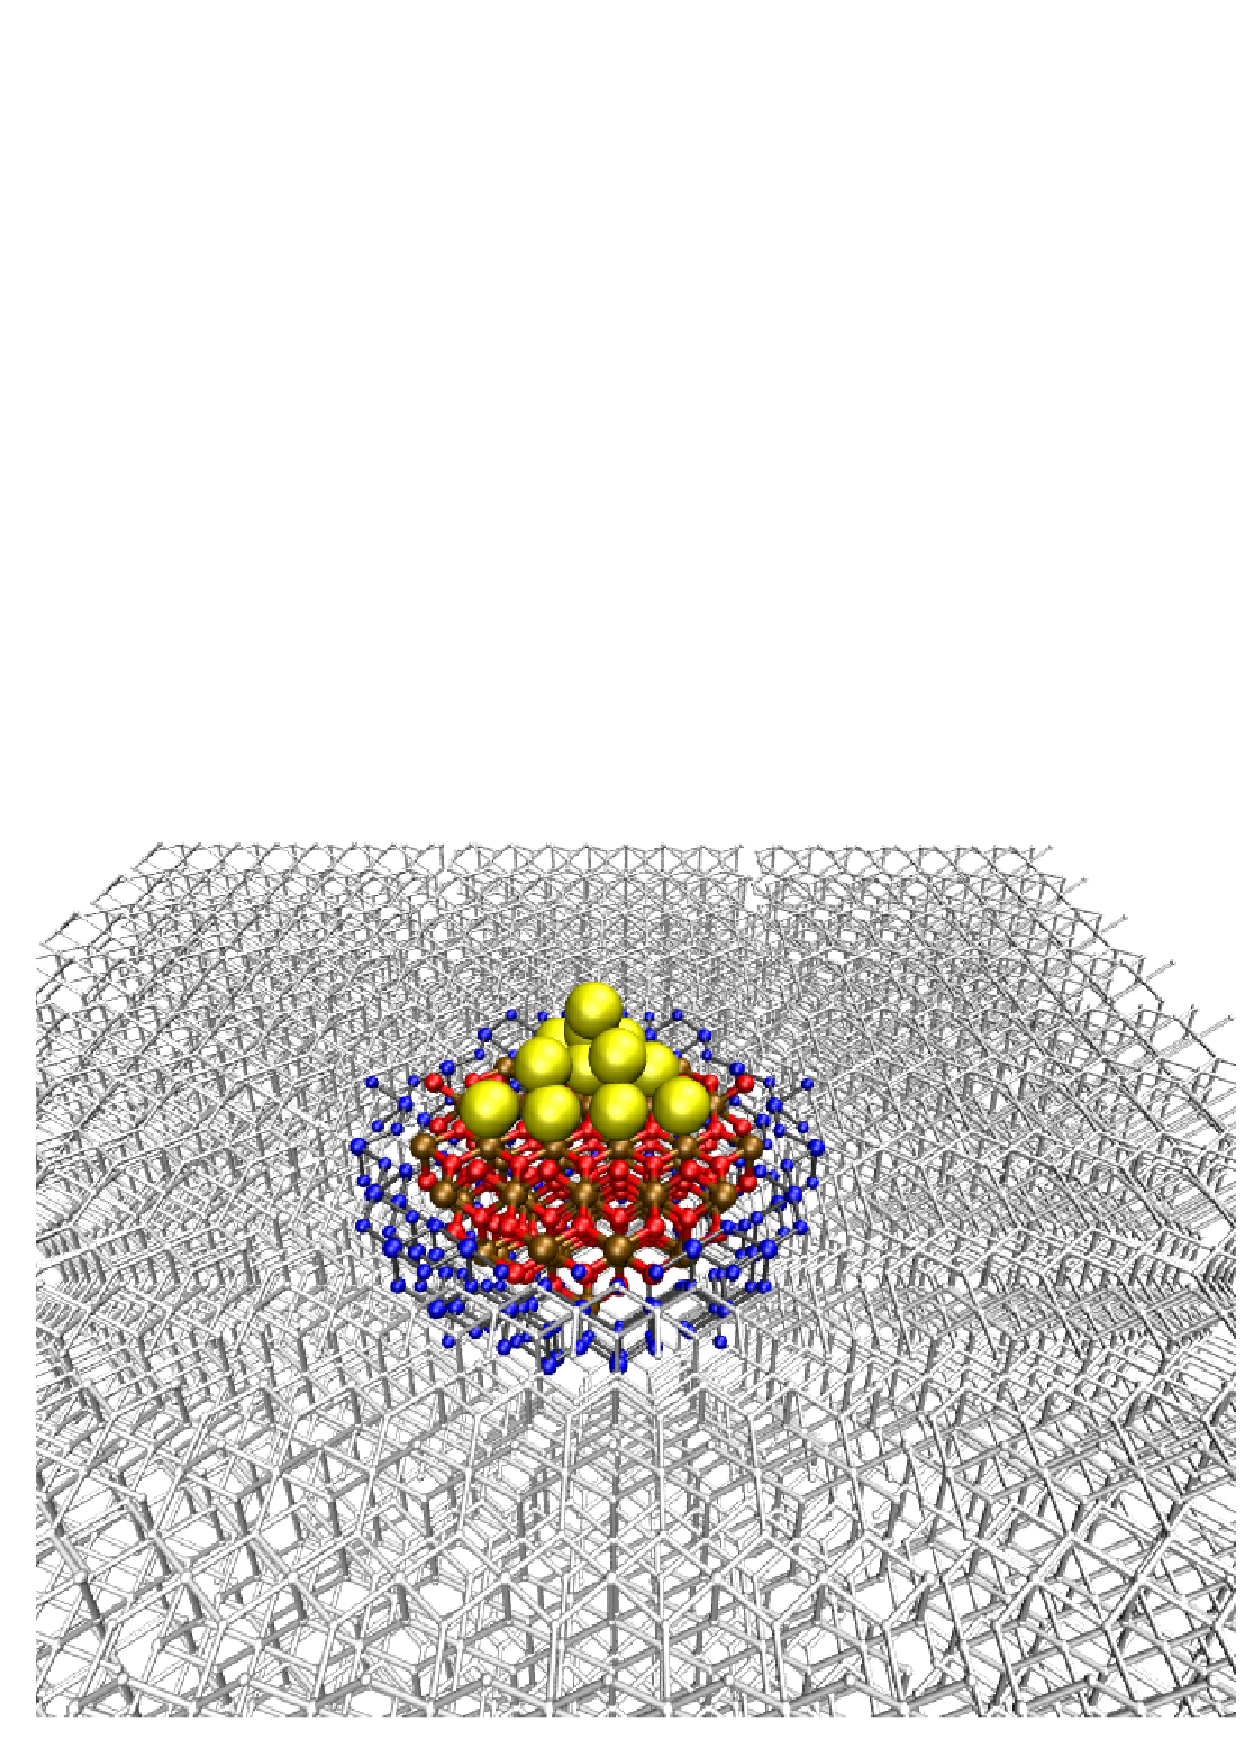
\includegraphics[width=0.7\textwidth]{qmmm}
  \caption{Example for QM/MM setup: $Au_n@TiO_2$. The adsorbed cluster and direct substrate vicinity defines the QM-region.
The far field surrounding (grey particles) pictures a monopole field with formal charges (4+ for Ti and 2- for O). In the blue 
region, oxygen particles are still represented as monopoles, however Ti-cations are described with ionic pseudopotentials.}
  \label{fig:qmmm_embedding}
\end{figure}

 
The QM/MM approach has the huge advantage ultimately also being capable to efficiently 
deal with \textbf{charged} systems, which will be a fundamental asset for the 
description of surface electrochemistry or photo-induced catalysis.


\emph{QM/MM embedding is not applicable for metal substrates for physical reasons.}



% \emph{This functionality is not yet available for periodic systems.}

\newpage

\subsection*{Tags for \texttt{geometry.in}:}


\keydefinition{pseudocore}{geometry.in}
{
  \noindent
  Usage: \keyword{pseudocore} \option{x} \option{y} \option{z}
    \option{species} \\[1.0ex] 
  Purpose: Places the center of a pseudopotential at a
    specified location. \\[1.0ex]
  \option{x} : $x$ coordinate of the pseudocore. \\
  \option{y} : $y$ coordinate of the pseudocore. \\
  \option{z} : $z$ coordinate of the pseudocore. \\
  \option{species} : string defining the name of the pseudoized species; this needs to correspond to name specified in control.in . \\
}

The keyword \keyword{pseudocore} should be used for those particles
replaced by pseudopotentials, so cations. Anions are to be treated simply
as monopoles, employing the \keyword{multipole} infrastructure.

% \vspace{2cm}
% \begin{center}
% !!! At one point I should add a script for constructing a divided surface!!!\end{center}
% 
% \newpage

\subsection*{Tags for general section of \texttt{control.in}:}

Only species data concerning the pseudoized species mentioned in \texttt{geometry.in} 
need to be appended in the \texttt{control.in}.
Accept for some mandatory changes (listed below) those species data are essentially the same 
as you can find them in the species\_default folder. E.g. if you want to pseudoize for example titanium, 
take the $Ti$ default file as a template. However, \textbf{the pseudoized species must not have any basis functions 
accept for the minimal basis}. The minimal basis in needed to construct the integration weights, however in order 
to exclude the minimal basis from the actual quantum chemical calculation, the flag 
\subkeyword{species}{include\_min\_basis} needs to be set to \texttt{.false.}.


Although nomenclature is misleading as it is chosen at the moment, you do NOT need the \keyword{qmmm}
in order to make QM/MM embedding work. 




\begin{figure}[hb]
  \small
  \begin{verbatim}


[...]
  species        Ti_pseudo
#     global species definitions
    nucleus             22
    mass                47.867

    pseudo              Ti.cpi
    pp_charge           4.
    pp_local_component     1
    nonlinear_core      .false.

    include_min_basis .false.


[...]

  \end{verbatim}
  \normalsize

  \vspace*{-4.0ex}

  \caption{\label{Fig:control.in_qmmm}
Species data for a pseudoized titanium atom. Starting from the default species files 
only a few flags need to be added and the basis functions (accept the minimal basis) 
need to be removed.
  }
\end{figure}


Similar to all-electron \subkeyword{species}{atom}, FHI-aims expects all atom specifications  
like \subkeyword{species}{mass}, \subkeyword{species}{nucleus}, information for the integration grid etc.
Some additional flags need to be set that FHI-aims is able to realize them as pseudoized species.  

\subkeydefinition{species}{pseudo}{control.in}
{
  \noindent
  Usage: \subkeyword{species}{pseudo} \option{string} \\[1.0ex]
  Purpose: Parses the name of file the Kleinman-Bylander pseudopotential 
is written in \\[1.0ex]
  \option{string} name of file\\
}

FHI-aims expects the pseudopotential file to be in a specific formatting, namely the 
output format *.cpi of the generator program FHI98PP \cite{FuchsFHI98PP}.
FHI98PP expects this file to be in the same folder as control.in and geometry.in.

\subkeydefinition{species}{pp\_charge}{control.in}
{
   \noindent
   Usage: \subkeyword{species}{pp\_charge} \option{value} \\[1.0ex]
   Purpose: Specifies the charge of the pseudoized ion. \\[1.0ex]
   \option{value:} any real value is allowed\\
 }

 \subkeyword{species}{pp\_charge} must be the charge which has been
 set in the generation of the pseudopotential and equals the number of
 pseudoized valence electrons.  This parameter is needed for the far
 field extrapolation of the pseudopotential.


\subkeydefinition{species}{pp\_local\_component}{control.in}
{
  \noindent
  Usage: \subkeyword{species}{pp\_local\_component} \option{value} \\[1.0ex]
  Purpose: Specifies which l-channel of the pseudopotential should act as the local component.
Find a detailed theoretical background in \cite{FuchsFHI98PP}. \\[1.0ex]
  \option{value:} integer value\\
}

The choice which l-channel should be the local component is essential for the performance 
of the pseudopotentials. Again, read \cite{FuchsFHI98PP} for further help.


\subkeydefinition{species}{ nonlinear\_core}{control.in}
{
  \noindent
  Usage: \subkeyword{species}{ nonlinear\_core} \option{flag} \\[1.0ex]
  Purpose: when .true. FHI-aims expects and reads in a partial core density (and partial core density gradient)
 from the pseudopotential input file to take account of nonlocal core correction \cite{Louie1982}. \\[1.0ex]
  \option{flag} is a logical expression, either .true. or .false. Default: .false.\\
}



\section{Continuum Solvation Methods}
\label{Sec:ContSolvMethods}

Continuum or implicit solvation methods provide a fast way the influence of solvents and electrolytes on chemical reactions. Currently, FHI-aims supports two models which have different strengths and capabilities which are summarized in Table \ref{tab:ImpSolvMethods}. Both models place a dielectric continuum outside the charge distribution modeling the polarizibility of the solvent. Differences arise in the solvation cavity definition. The Multipole Expansion (MPE) implicit solvation method separates the FHI-aims grid into two domains and couples them via electrostatic boundary conditions. It therefore in fact solves two coupled Poisson equations with different dielectric permittivities. The Finite ion-size and Stern layer modified Poisson-Boltzmann (SMPB) method solves a single Poisson equation on the full FHI-aims integration grid by defining a smooth dielectric permittivity function.  In general, the accuracy of the evaluation of solvation energies is expected to be similar. In fact, both methods  merge into each other if the dielectric transition in the SMPB model is turned into a sharp step function. On top of this ion-free implicit solvation model, the SMPB approach also supports the modeling of finite ionic strengths in the solution.

The MPE solvation model is the faster one of both approaches with only a small overhead with respect to vacuum calculations. The overhead of both implicit solvation methods is reduced, when performing expensive hybrid calculations, since the actual time for the implicit solvation calculations does not vary with the functional.

\begin{table}[htb]
\centering
 \begin{tabular}{ l | c | c }
   & \textbf{MPE} & \textbf{SMPB}\\
  \hline		
  Solvent Parametrizations  & H$_2$O (N,C) & H$_2$O (N,C), CH$_3$OH (N,C)\\
    & & (more in work)\\
  Dissolved ions/salt & no & yes (SMPB/LPB)\\
  Salt Parametrizations & -- & Aq. Monoval. Salt Solutions\\
  CPU speed  & fast & moderate \\
  Forces & no & yes\\
  PBCs & no & no (in work)\\
  Developers	 & \href{markus.sinstein@mytum.de}{\underline{Markus Sinstein}} & \href{mailto:sringe@stanford.edu}{\underline{Stefan Ringe}}\\ 
  & & \small{Christoph Muschielok, Marvin H. Lechner} \\
  \hline  
\end{tabular}
 \caption{Comparison of the two implicit solvation methods in FHI-aims. Parameter sets for the MPE method are available in ref. \cite{Sinstein2017_MPE}, for the SMPB method in ref. \cite{Andreussi2012} and \cite{Dupont2013-bc} (parameters for methanol as more solvents in current work). N and C indicate parameter sets fitted for neutral and charged solutes, respectively.}
 \label{tab:ImpSolvMethods}
\end{table}

In the following, both models are summarized and the key input parameters presented.

\subsection{MPE Implicit Solvent Model}
\label{Sec:MultiPoleExpansion}

\emph{This is an experimental feature which is still under development. 
Do not rely on properties calculated by this method! 
Please contact the authors for further details.}

\emph{This functionality is not yet available for periodic systems.}

\emph{The current implementation does not have analytical forces yet.}

\emph{Generally, when combining MPE with other functionality, you should know what you are doing. No specific interactions with other methods beyond single point DFT are implemented, so only methods which do not interfere with MPE are safe to use.}

The simulation of a solvent in a quantum mechanical calculation can, in principle, be done in two ways. One way is to include explicit solvent molecules in the calculation. This straightforward approach usually requires molecular dynamics (MD) simulations in order to yield thermodynamically meaningful observables as e.g.~solvation free energies.

The second way is to average the effect of the solvent and treat it as a continuum which responds to the electrostatic potential created by the solute, i.e.~the entity that is to be solvated. There are several flavors to this comparatively inexpensive approximation, e.g.~
the polarizable continuum model (PCM) \cite{Mennucci02}, 
the conductor like screening model (COSMO) \cite{Klamt93}, 
the self-consistent continuum solvation (SCCS) model \cite{Andreussi2012}, 
the ``SMx'' models \cite{Cramer2008_SM8,Marenich2009_SMD,Marenich2013_SM12}, 
or CMIRSv1.1 \cite{You2016_CMIRS11} 
to name some of the more popular ones. 
Statistical sampling then only needs to be performed for the degrees of freedom of the solute which obviously makes it computationally much cheaper. 

In general, the necessary integration of the solvent's degrees of freedom beforehand leads to a problem where one now needs to solve a generalized Poisson's equation, 
\begin{align}
\Del \left( \varepsilon_0\varepsilon(\Vect{r}) \Del \Phi(\Vect{r}) \right) = - 4\pi \varrho(\Vect{r}) \label{eq:mpe_gen_poisson}, 
\end{align}
to obtain the electrostatic potential $\Phi(\Vect{r})$ created by the total charge density $\varrho(\Vect{r})$ which now accounts for the electrostatic polarization potential of the solvent (often called ``reaction field''). 
Eq.~\ref{eq:mpe_gen_poisson} contains a spatially dependent dielectric permittivity function $\varepsilon(\Vect{r})$ in contrast to the regular Poisson's equation,
\begin{align}
\Del \left( \varepsilon_0 \Del \Phi_\mathrm{H}(\Vect{r}) \right) = - 4\pi \varrho(\Vect{r}) \label{eq:mpe_poisson}, 
\end{align}
which is solved in a regular DFT calculation in every step of the SCF cycle to get the Hartree potential $\Phi_\mathrm{H}$. 

As outlined in more detail in Ref.~\cite{Sinstein2017_MPE}, the multipole expansion (MPE) implicit solvent model offers an efficient way of solving Eq.~\ref{eq:mpe_gen_poisson} based on the knowledge of the Hartree potential $\Phi_\mathrm{H}$ readily available from a splined representation in FHI-aims (cf.~Sec.~\ref{Sec:Hartree}) via least-squares fitting instead of integration. 
The dielectric function $\varepsilon(\Vect{r})$ here needs to be a step-function in 3D-space where the following boundary conditions apply at the step ($\Vect{n}$ denotes the normal direction to the interface): 
\begin{subequations}
\begin{align}
\Phi_+ = \Phi_- \label{eq:mpe_bc1_gen}
\end{align}
\begin{align}
\Vect{n} \cdot \varepsilon_+ \Del \Phi_+ = \Vect{n} \cdot \varepsilon_- \Del \Phi_- \label{eq:mpe_bc2_gen}
\end{align}
\end{subequations}

Then, the above equations are discretized in two ways: 
\begin{itemize}
\item The potentials $\Phi_+$ and $\Phi_-$ are expressed in a truncated multipole series with expansion orders $l_\mathrm{max,R}$ and $l_\mathrm{max,O}$, and
\item equations~\ref{eq:mpe_bc1_gen} and \ref{eq:mpe_bc2_gen} are evaluated at $N$ points on the interface manifold. 
\end{itemize}
Thereby, $N$ is chosen such that the resulting system of linear equations (SLE) is overdetermined (typically by a factor of two to three). 


%\newpage


\subsubsection*{Tags for general subsection of \texttt{control.in}:}

The keywords controlling the MPE module are divided into four categories:
\begin{itemize}
\item[elementary] These are the most important keywords---some are even mandatory---which likely need to be specified for every calculation. 
\item[convergence] Here, the most important convergence parameters are collected which should be checked before doing (large scale) production runs. 
\item[expert] These settings should only be modified by an experienced user as they allow quite profound modifications. 
\item[debug] Debug settings are intended to give valuable insight for developers into intermediate results. 
\end{itemize}

The authors strongly encourage new users to try out ``elementary'' and ``convergence'' settings first in order to gather some experience with the MPE implementation before any modifications of other settings are made.

\paragraph{elementary}

\keydefinition{solvent}{control.in}
{
  \noindent
  Usage: \keyword{solvent} \option{method} \\[1.0ex] 
  Purpose: Specifies the desired implicit solvent model. \\[1.0ex]
  \option{method} is a string which specifies the implicit solvent method; 
    currently, \option{mpe} (the method presented above) and 
    \option{mpb} (cf.~Sec.~\ref{Sec:ModifiedPoissonBoltzmann}) 
    are supported. \\
}


\keydefinition{mpe\_solvent\_permittivity}{control.in}
{
  \noindent
  Usage: \keyword{mpe\_solvent\_permittivity} \option{epsilon} \\[1.0ex] 
  Purpose: Specifies the dielectric constant of the bulk solvent. \\[1.0ex]
  \option{epsilon} is a positive real number equal to the macroscopic 
    dielectric constant of the solvent. Default: \option{1.0} \\
}


\keydefinition{isc\_cavity\_type}{control.in}
{
  \noindent
  Usage: \keyword{isc\_cavity\_type} \option{type} \\[1.0ex] 
  Purpose: This keyword controls the model used to sample 
    the implicit solvent cavity for the MPE method. 
    Depending on \option{type}, further flags (or even lines) might be 
    necessary. Those are explained below. \\[1.0ex]
  Options: Currently supported options are 
    \option{overlapping\_spheres}, 
    \option{rho\_free}, 
    \option{rho\_multipole\_static}, 
    and \option{rho\_multipole\_dynamic}. \\
}

\subkeydefinition{isc\_cavity\_type}{rho\_free}{control.in}
{
  \noindent
  Usage: \keyword{isc\_cavity\_type} 
    \subkeyword{isc\_cavity\_type}{rho\_free} 
    \option{rho\_iso} \\[1.0ex] 
  Purpose: Constructs the cavity as an iso-density surface of the 
    superposed electron density of the neutral, free atoms in
    the solute. \\[1.0ex]
  \option{rho\_iso} is a positive real number specifying the 
    desired iso-density value in units of 
    \si{\elementarycharge\per\cubic\angstrom} .
}

\subkeydefinition{isc\_cavity\_type}{rho\_multipole\_static}{control.in}
{
  \noindent
  Usage: \keyword{isc\_cavity\_type} 
    \subkeyword{isc\_cavity\_type}{rho\_multipole\_static} 
    \option{rho\_iso} \\[1.0ex] 
  Purpose: Constructs the cavity as an iso-density surface of the 
    \emph{initial} (multipole-expanded) electron density of the solute. \\[1.0ex]
  \option{rho\_iso} is a positive real number specifying the 
    desired iso-density value in units of 
    \si{\elementarycharge\per\cubic\angstrom} .
}
Note, that \emph{initial} electron density in this context means 
the electron density at the time of the first call to the cavity 
generation routine is used. Thus, the shape of the cavity depends 
on several other parameters of the calculation, such as after how 
many SCF steps the cavity is built (mainly influenced by 
\option{mpe\_skip\_first\_n\_scf\_steps}) or which restart 
information was used---if any. 
In any case, the cavity shape then stays constant throughout 
the whole calculation. 
Although care should be taken due to the various influences on the 
cavity definition, this cavity type can be used as a cheaper 
alternative to the fully self-consistent cavity when the 
initialization is based on the converged density of the vacuum 
calculation, i.e.~restarting from it, as the polarization 
potential often (not always!) has a minor influence on the 
electron density. 

\subkeydefinition{isc\_cavity\_type}{rho\_multipole\_dynamic}{control.in}
{
  \noindent
  Usage: \keyword{isc\_cavity\_type} 
    \subkeyword{isc\_cavity\_type}{rho\_multipole\_dynamic} 
    \option{rho\_iso} \\[1.0ex] 
  Purpose: Constructs the cavity as an iso-density surface of the 
    \emph{self-consistent} (multipole-expanded) electron density 
    of the solute. \\[1.0ex]
  \option{rho\_iso} is a positive real number specifying the 
    desired iso-density value in units of 
    \si{\elementarycharge\per\cubic\angstrom} .
}
With this method, the cavity is updated to the current electron 
density in every SCF step. This also means that the MPE equations 
have to be solved in every SCF step making it computationally 
more expensive. 

\subkeydefinition{isc\_cavity\_type}{overlapping\_spheres}{control.in}
{
  \noindent
  Usage: \keyword{isc\_cavity\_type} 
    \subkeyword{isc\_cavity\_type}{overlapping\_spheres} 
    \option{type} \option{value} \\[1.0ex] 
  Purpose: Constructs the cavity as a superposition of overlapping 
    spheres around all atoms. \\[1.0ex]
  \option{type} specifies how the radii of the atomic spheres 
    are determined.
    \begin{itemize}
    \item \option{radius}: all spheres have the same radius
      given by \option{value} in units of \si{\angstrom};
    \item \option{rho}: the atomic spheres are iso-density surfaces 
      based on the electron density of the isolated, neutral atom 
      with an iso-value of \option{value} in units of 
      \si{\elementarycharge\per\cubic\angstrom} .
    \end{itemize} %\\
  \option{value} is a real number whose meaning and units
    depend on the choice of \option{radius} (see above). \\
}
\emph{WARNING}: The usage of this cavity type is strongly discouraged! 
It has been helpful in the development to analyze the cavity sampling 
process itself. The resulting cavities, however, are almost certainly 
not smooth and were never intended to be used in production calculations.
When used with the MPE model, the whole calculation is prone to numerical 
problems and the results are very often unphysical. 
Instead, use the \option{rho\_free} type that builds the cavity based on the
superposition of atomic densities (which is again smooth) or use other 
types based on the (self-consistent) electron density of the solute. 


\keydefinition{mpe\_nonelectrostatic\_model}{control.in}
{
  \noindent
  Usage: \keyword{mpe\_nonelectrostatic\_model} \option{model} \\[1.0ex] 
  Purpose: This keyword controls any additional, ``non-electrostatic'' terms 
    not included in the purely electrostatic treatment of the solvent. 
    Depending on \option{model}, further flags (or even lines) might be 
    necessary. Those are explained below. \\[1.0ex]
  Options: Currently, only \option{linear\_OV} is supported. \\
}

\subkeydefinition{mpe\_nonelectrostatic\_model}{linear\_OV}{control.in}
{
  \noindent
  Usage: \keyword{mpe\_nonelectrostatic\_model} 
    \subkeyword{mpe\_nonelectrostatic\_model}{linear\_OV} 
    \option{$\alpha$} \option{$\beta$} \\[1.0ex] 
  Purpose: Corrects the total energy term by $\alpha O + \beta V$ 
    where $O$ is the surface area of the cavity and
    $V$ its volume. \\[1.0ex]
  \option{$\alpha$} is a real number in units of 
    \si{\electronvolt\per\angstrom\squared}. 
    Default: \option{0.0} \\
  \option{$\beta$} is a real number in units of 
    \si{\electronvolt\per\cubic\angstrom}. 
    Default: \option{0.0} \\
}
This non-electrostatic model is in principle identical to the one 
proposed by Andreussi~\emph{et al.} \cite{Andreussi2012}. 
Note, however, that the surface tension of the solvent is here 
included in the parameter $\alpha$. 


\paragraph{convergence}

\keydefinition{mpe\_lmax\_rf}{control.in}
{
  \noindent
  Usage: \keyword{mpe\_lmax\_rf} \option{lmax} \\[1.0ex] 
  Purpose: Specifies the expansion order of the 
    polarization potential aka reaction field 
    inside the cavity. \\[1.0ex]
  \option{lmax} is a non-negative integer number. 
    Default: \option{8} \\
}
This is a critical convergence parameter of 
the MPE model. You should never forget to test 
convergence with respect to this parameter before 
doing production runs. 
For small organic molecules, the largest and 
successfully tested expansion order so far has been 14. 
Note, however, that numerical problems might arise when 
choosing even larger values for \option{lmax} or 
when going to larger systems. 

\keydefinition{mpe\_lmax\_ep}{control.in}
{
  \noindent
  Usage: \keyword{mpe\_lmax\_ep} \option{lmax} \\[1.0ex] 
  Purpose: Specifies the expansion order of the 
    polarization potential aka reaction field 
    outside of the cavity. \\[1.0ex]
  \option{lmax} is a non-negative integer number. 
    Default: maximum value of 
      \subkeyword{species}{l\_hartree} for all
      species. \\
}
This parameter is similar to but usually less critical 
than \keyword{mpe\_lmax\_rf}. However, careful convergence 
tests with respect to this parameter before 
doing production runs is advisable since this parameter 
dictates the size of the MPE matrix equation. 
Choosing larger values than the default should 
usually have little to no impact on the results. 


\keydefinition{mpe\_degree\_of\_determination}{control.in}
{
  \noindent
  Usage: \keyword{mpe\_degree\_of\_determination} 
    \option{dod} \\[1.0ex] 
  Purpose: Defines the desired ratio of number of 
    rows to columns in left-hand side matrix of the 
    MPE equation. \\[1.0ex]
  \option{dod} is a real number $\ge 1.0$. 
    Default: \option{5.0} \\
}
For the very limited (!) number of applications of the MPE 
method so far, the default value of 5.0 has been a save choice. 
However, you should never forget to test convergence with 
respect to this parameter before doing production runs. 
Note, that the requested degree of determination can only 
very approximately be reached. This can lead to an under-
determination of the MPE equations and a subsequent 
termination of the program when values for \option{dod} 
very close to 1 are chosen.


\keydefinition{mpe\_tol\_adjR2}{control.in}
{
  \noindent
  Usage: \keyword{mpe\_tol\_adjR2}
    \option{tol} \\[1.0ex]
  Purpose: Defines the tolerance for the adjusted coefficient
    of determination $\bar{R}^2$ of the solved MPE equations.
    Will abort if $\bar{R}^2 < 1 - tol$. \\[1.0ex]
  \option{tol} is a real number between $0.0$ and $1.0$.
    Default: \option{0.075} \\
}
The MPE equations are sometimes not solvable in the regular
solid harmonic basis used for the reaction field. This is the case
especially for large molecules. A low $\bar{R}^2$ indicates such
a bad solution. In some cases increasing \keyword{mpe\_lmax\_rf}
helps, but there are pathologic cases where increasing
\keyword{mpe\_lmax\_rf} leads to a perpetual decrease in
$\Delta_\text{solv}^\text{el}G$ without ever converging.

For $\bar{R}^2 < 0.925$ it is likely that less than 90\%
of $\Delta_\text{solv}^\text{el}G$ are captured. This is however
based on experience from a limited number of cases. Feedback to
the developers (\href{mailto:jakob.filser@tum.de}{\underline{jakob.filser@tum.de}}) will be appreciated!

\keydefinition{mpe\_tol\_adjR2\_wait\_scf}{control.in}
{
  \noindent
  Usage: \keyword{mpe\_tol\_adjR2\_wait\_scf}
    \option{bool} \\[1.0ex]
  Purpose: If \option{.true.}, will wait until the SCF cycle is
  converged before it is checked whether $\bar{R}^2 < 1 - tol$. \\[1.0ex]
    Default: \option{.false.} \\
}
Although MPE does not actively try to converge, $\bar{R}^2$
tends to improve during the SCF procedure. Setting
\keyword{mpe\_tol\_adjR2\_wait\_scf} can thus help borderline cases
converge, at the cost of spending the full computation time
of the SCF procedure on a calculation that might ultimately fail.

\paragraph{expert}

\keydefinition{mpe\_factorization\_type}{control.in}
{
  \noindent
  Usage: \keyword{mpe\_factorization\_type} \option{type} \\[1.0ex] 
  Purpose: Defines the numerical method used to factorize the 
    left-hand side of the MPE equations as the first step to 
    the numerical solution. \\[1.0ex]
  \option{type} can be chosen from: \option{qr}, \option{qr+svd}, 
    and \option{svd}. Default: \option{qr+svd} \\
}
\emph{The option} \option{qr} \emph{is temporarily disabled until
$\bar{R}^2$ is implemented for this case!}

The default behavior is to perform a QR factorization with a 
singular value decomposition (SVD) on top. This allows to 
robustly solve the MPE equation via the pseudo-inverse of 
the left-hand side. 

\emph{Be careful!} Using the (non rank-revealing) QR 
factorization alone can fail when the left-hand side is 
rank deficient which can easily happen---especially 
for large expansion orders 
\keyword{mpe\_lmax\_rf} and/or \keyword{mpe\_lmax\_ep}! 
On the other hand, \option{svd} does not necessarily mean that 
no QR factorization is performed as this (at least for 
the parallel implementation) depends on the (Sca)LAPACK 
driver routine used. 


\keydefinition{mpe\_f\_sparsity\_threshold}{control.in}
{
  \noindent
  Usage: \keyword{mpe\_f\_sparsity\_threshold} 
    \option{threshold} \\[1.0ex] 
  Purpose: Can potentially speed up the evaluation of 
    the reaction field on the integration grid by 
    neglecting all its coefficients smaller than
    \option{threshold}. \\[1.0ex]
  \option{threshold} is a non-negative real number. 
    Default: \option{0.0} \\
}
Speed in this case usually comes at the price of 
sacrificing accuracy, i.e. it should always be tested 
if the results are still sufficiently accurate. 
Moreover, a large threshold might cause instabilities 
in the SCF cycle!


\keydefinition{mpe\_skip\_first\_n\_scf\_steps}{control.in}
{
  \noindent
  Usage: \keyword{mpe\_skip\_first\_n\_scf\_steps} \option{n} \\[1.0ex] 
  Purpose: Switch off (or rather, do not switch on) the 
    MPE implicit solvent model in the first 
    \option{n} SCF steps. \\[1.0ex]
  \option{n} is a non-negative integer value. Default: \option{0} \\
}
\emph{Attention:} No check is performed whether the MPE 
has been switched on before the end of the run! For example, 
the implicit solvent will be ignored when the SCF cycle 
happens to converge in \option{n} steps or less. 
Note that the counting of SCF steps can deviate from the 
regular FHI-aims counting as the re-initialization 
from restart is also counted as one SCF step. 

\keydefinition{mpe\_n\_centers\_ep}{control.in}
{
  \noindent
  Usage: \keyword{mpe\_n\_centers\_ep} \option{n} \\[1.0ex] 
  Purpose: Defines the number of centers used 
    for the expansion of the polarization potential 
    outside of the cavity. \\[1.0ex]
  \option{n} is a positive integer number. 
    Default: number of centers for the Hartree 
    potential expansion (cf.~\ref{Sec:Hartree}) \\
}
The first \option{n} centers defined in 
\texttt{geometry.in} are used as expansion centers. 
The default is to use all of them. Only change this 
value if you fully understand what you are doing and 
why you want to do this! 


\keydefinition{mpe\_n\_boundary\_conditions}{control.in}
{
  \noindent
  Usage: \keyword{mpe\_n\_boundary\_conditions} \option{nbc} \\[1.0ex] 
  Purpose: Determines the number of boundary conditions 
    imposed at every point on the cavity interface. \\[1.0ex]
  Valid choices for \option{nbc} are 2 and 4. Default: \option{2} \\
}
As outlined in Ref.~\cite{Sinstein2017_MPE}, there are at least 
two more boundary conditions other than Eqns.~\ref{eq:mpe_bc1_gen} 
and \ref{eq:mpe_bc2_gen} that can be imposed on the electrostatic 
potential / field / flux at a dielectric interface. 
The default is to enforce continuity of the potential and 
continuity of the dielectric flux perpendicular to the interface, 
i.e.~\option{nbc} equals 2. 
Furthermore, continuity of the electric field parallel to the 
interface can be imposed, i.e.~\option{nbc} equals 4. 
However, this should automatically be satisfied by the former 
two boundary conditions and---in the best case---only leads to 
a higher order correction of the fit. 
\emph{Warning:} The non-default has not been tested thoroughly. 
Verify your results carefully when using it! 


\keydefinition{isc\_calculate\_surface\_and\_volume}{control.in}
{
  \noindent
  Usage: \keyword{isc\_calculate\_surface\_and\_volume} \option{bool} \\[1.0ex] 
  Purpose: Determines whether the surface area and volume 
    of the cavity are calculated. \\[1.0ex]
  \option{bool} is of Boolean type. Default: \option{.true.} \\
}
As the only currently implemented \keyword{mpe\_nonelectrostatic\_model} 
\subkeyword{mpe\_nonelectrostatic\_model}{linear\_OV} requires 
the calculated measures, this flag is automatically turned on 
when it has been turned off but is needed. 

\keydefinition{isc\_surface\_curvature\_correction}{control.in}
{
  \noindent
  Usage: \keyword{isc\_surface\_curvature\_correction} \option{bool} \\[1.0ex] 
  Purpose: When this flag is turned on, the calculated surface 
    area (and volume) of the cavity is approximately corrected 
    for the cavity curvature. \\[1.0ex]
  \option{bool} is of Boolean type. Default: \option{.true.} \\
}
The effect of this keyword is usually rather negligible. 
For more details regarding the correction, please consult 
Ref.~\cite{Sinstein2017_MPE}. 


\keydefinition{isc\_rho\_rel\_deviation\_threshold}{control.in}
{
  \noindent
  Usage: \keyword{isc\_rho\_rel\_deviation\_threshold} 
    \option{threshold} \\[1.0ex] 
  Purpose: Defines the convergence criterion of the 
    cavity generation process: The walker dynamics simulation 
    is run until the density values for all walkers deviate 
    from the chosen iso value by at most \option{threshold}. \\[1.0ex]
  \option{threshold} is a small, positive real number. 
    Default: \option{\SI{1e-3}{}} \\
}
This keyword is only applicable for an \keyword{isc\_cavity\_type} 
defined by an iso-density value. 

\keydefinition{isc\_max\_dyn\_steps}{control.in}
{
  \noindent
  Usage: \keyword{isc\_max\_dyn\_steps} \option{num} \\[1.0ex] 
  Purpose: Determines the maximum number of allowed steps 
    to reach convergence of the walker dynamics simulation 
    in the cavity creation process. \\[1.0ex]
  \option{num} is a positive integer number. Default: \option{300} \\
}

\keydefinition{isc\_try\_restore\_convergence}{control.in}
{
  \noindent
  Usage: \keyword{isc\_try\_restore\_convergence} \option{bool} \\[1.0ex] 
  Purpose: When convergence of the cavity creation dynamics run 
    could not be achieved within the number of allowed steps 
    specified by \keyword{isc\_max\_dyn\_steps}, this flag allows 
    to enforce convergence by simply deleting all walkers 
    not satisfying the convergence criterion given by 
    \keyword{isc\_rho\_rel\_deviation\_threshold}. \\[1.0ex]
  \option{bool} is of Boolean type. Default: \option{.false.} \\
}
Although a simple check is done to stop the calculation when 
too many walkers do not satisfy the convergence criterion, one 
should always manually checking the resulting cavity for 
larger holes that might result from the deletion of walkers 
which can lead to a bad estimate of the cavity's surface area 
and volume and maybe also have an impact on the quality of 
the polarization potential. 

\keydefinition{isc\_kill\_ratio}{control.in}
{
  \noindent
  Usage: \keyword{isc\_kill\_ratio} \option{fraction} \\[1.0ex] 
  Purpose: This keyword can be helpful when the walker 
    dynamics run does not converge due to trapped walkers 
    by killing the worst \option{fraction} of walkers 
    at each neighbor list update step (also see 
    \keyword{isc\_update\_nlist\_interval}). \\[1.0ex]
  \option{fraction} is a non-negative real number
    much smaller than 1. Default: \option{0.0} \\
}
As the number of possibly trapped walkers depends a lot 
on the shape of the electron density, it is rather 
difficult to give a recommendation about a sensible 
value for \option{fraction}. In case walkers 
get stuck, we propose to use a rather conservative 
kill ratio of $~\SI{1e-3}{}$ and only increase it 
if necessary. 

\keydefinition{isc\_update\_nlist\_interval}{control.in}
{
  \noindent
  Usage: \keyword{isc\_update\_nlist\_interval} \option{num} \\[1.0ex] 
  Purpose: This keyword triggers a re-evaluation of the 
    neighbor lists in the density walkers dynamics simulation 
    after every \option{num} steps. \\[1.0ex]
  \option{num} is a positive integer number. Default: \option{50} \\
}

\keydefinition{isc\_dynamics\_friction}{control.in}
{
  \noindent
  Usage: \keyword{isc\_dynamics\_friction} \option{fric} \\[1.0ex] 
  Purpose: The value of \option{fric} determines how much 
    ``kinetic energy'' is removed from the walkers in 
    every step of the simulations via a simple  
    velocity scaling. \\[1.0ex]
  \option{fric} is a real number between 0 and 1. 
    Default: \option{0.1} \\
}
A value of 0 for \option{fric} means that no energy is 
removed from the system which may lead to a bad convergence 
behavior. On the other hand, a value of 1 means that all 
kinetic energy is removed at each step which tends to 
slow down the rate of convergence. 

\keydefinition{isc\_dt}{control.in}
{
  \noindent
  Usage: \keyword{isc\_dt} \option{delta} \\[1.0ex] 
  Purpose: Determines the ``time'' step of the 
    walker dynamics simulation. \\[1.0ex]
  \option{delta} is a positive real number. Default: \option{0.1} \\
}
Note: Since this is no actual physical quantity, arbitrary 
time units are used. 

\keydefinition{isc\_rho\_k}{control.in}
{
  \noindent
  Usage: \keyword{isc\_rho\_k} \option{k} \\[1.0ex] 
  Purpose: Determines the force constant \option{k} 
    for the ``density'' force, i.e.~the harmonic force 
    that pulls the walkers along the density gradient 
    to the specified iso-density value. \\[1.0ex]
  \option{k} is a positive real number. Default: \option{1.0} \\
}
Note: Since this is no actual physical quantity, arbitrary 
time units are used. 

\keydefinition{isc\_rep\_k}{control.in}
{
  \noindent
  Usage: \keyword{isc\_rep\_k} \option{k} \\[1.0ex] 
  Purpose: Determines the force constant \option{k} 
    for the repulsive interaction between walkers 
    perpendicular to the density gradient. \\[1.0ex]
  \option{k} is a positive real number. Default: \option{0.01} \\
}
Note: Since this is no actual physical quantity, arbitrary 
time units are used. 

\keydefinition{isc\_g\_k}{control.in}
{
  \noindent
  Usage: \keyword{isc\_g\_k} \option{k} \\[1.0ex] 
  Purpose: Determines the force constant \option{k} 
    for the ``gravitational'' force that drags walkers to the 
    center of gravity of the solute in case the local 
    density gradient is too small. \\[1.0ex]
  \option{k} is a positive real number. Default: \option{2.0} \\
}
Usually this should not happen, but when walkers move too 
far away from the solute, the density gradient becomes 
very small and its direction is unreliable due to numerical 
noise (see \keyword{isc\_gradient\_threshold}).
In this case, the walker is dragged to the center of the 
solute until the density gradient is again large enough. 
Note: Since this is no actual physical quantity, arbitrary 
time units are used. 

\keydefinition{isc\_gradient\_threshold}{control.in}
{
  \noindent
  Usage: \keyword{isc\_gradient\_threshold} 
    \option{thsq} \\[1.0ex] 
  Purpose: When the squared norm of the electron density 
    gradient at the position of a walker is less than 
    \option{thsq}, this gradient is considered unreliable. 
    Instead, a simple ``gravitational'' force towards the 
    center of the solute is applied. \\[1.0ex]
  \option{thsq} is a positive real number. 
    Default: \option{\SI{1e-8}{}} \\
}
The force constant of the ``gravitational'' force is 
determined by \keyword{isc\_g\_k}.


\paragraph{debug}

\keydefinition{mpe\_xml\_logging}{control.in}
{
  \noindent
  Usage: \keyword{mpe\_xml\_logging} \option{filename} 
    \option{level} \\[1.0ex] 
  Purpose: Controls the MPE module's internal XML logging 
    output. \\[1.0ex]
  \option{filename} specifies the name of the log file 
    to be written. Default: \option{mpe\_interface.xml} \\
  \option{level} defines the detail of the output. Supported 
    log levels are: \option{off}, \option{basic}, \option{medium}, and
    \option{detailed}. Default: \option{off} \\
}
This keyword is intended for debugging purposes. 
Note: Depending on the log level, the size of the output 
can become quite large. 


\keydefinition{isc\_cavity\_restart}{control.in}
{
  \noindent
  Usage: \keyword{isc\_cavity\_restart} \option{filename} \\[1.0ex] 
  Purpose: Read the solvation cavity from restart file 
    (if available) and write new cavity to same file. \\[1.0ex]
  \option{filename} is the name of the restart file. \\
}
Specifying this keyword is almost equivalent to specifying 
both \keyword{isc\_cavity\_restart\_read} and 
\keyword{isc\_cavity\_restart\_write} with the same 
\option{filename} option except that with 
\keyword{isc\_cavity\_restart} the program does not abort 
when there is no restart file to read from. \\
Note: This keyword is intended for debugging purposes. 
Do not rely on the current structure of the cavity restart 
file as it might change in the future. 

\keydefinition{isc\_cavity\_restart\_read}{control.in}
{
  \noindent
  Usage: \keyword{isc\_cavity\_restart\_read} \option{filename} \\[1.0ex] 
  Purpose: Read the solvation cavity from restart file 
    instead of constructing a new one. \\[1.0ex]
  \option{filename} is the name of the file (in \texttt{.xyz} format)
  containing the cavity points and normal vectors. Additionally, a file
  \texttt{<filename>.bin} is written which contains the entire cavity
  information in not human-readable form. While the primary purpose of the
  former is visualization, the latter is the actual restart file.\\
}
Note: This keyword is intended for debugging purposes. 
Do not rely on the current structure of the cavity restart 
file as it might change in the future. 

\keydefinition{isc\_cavity\_restart\_write}{control.in}
{
  \noindent
  Usage: \keyword{isc\_cavity\_restart\_write} \option{filename} \\[1.0ex] 
  Purpose: Write the cavity to the specified restart file
    once created. \\[1.0ex]
  \option{filename} is the name of the restart file (in \texttt{.xyz} format).
  If additionally \texttt{<filename>.bin} is present, the cavity is read from
  the latter instead. Note that the \texttt{.xyz} file has to be present in both
  cases. While this file itself is sufficient to create a cavity, only the
  \texttt{.bin} file allows for a fully deterministic restart.\\
}
Note: This keyword is intended for debugging purposes. 
Do not rely on the current structure of the cavity restart 
file as it might change in the future. 


\keydefinition{isc\_record\_cavity\_creation}{control.in}
{
  \noindent
  Usage: \keyword{isc\_record\_cavity\_creation} 
    \option{filename} \option{num} \\[1.0ex] 
  Purpose: Controls the output of snapshots during the 
    cavity generation process. When \option{num} 
    is positive, every \option{num} steps an XYZ snapshot 
    of the cavity is written to file \option{filename}. 
    For other choices of \option{num}, no output will 
    be generated. \\[1.0ex]
  \option{filename} is of type string. \\
  \option{num} is of type integer. Default: \option{0} \\
}
This keyword is intended for debugging purposes. Note that 
the size of the output file can become very large! 



\subsection{SMPB Implicit Electrolyte Model}
\label{Sec:ModifiedPoissonBoltzmann}

In FHI-aims, implicit solvation effects or electrolyte effects (z:z electrolytes) can be included by solving the Stern- and finite ion-size \emph{Modified Poisson-Boltzmann} equation (\emph{(S)MPBE}) in each SCF step:

\begin{equation}
\nabla \cdot \left[\varepsilon[n_{\rm el}(\bm{r})]\nabla v(\bm{r})\right] \;=\; -4\pi n_{\rm sol}(\bm{r}) - 4\pi n_\mathrm{ion}^\mathrm{MPB}(\bm{r}) \quad ,
\label{eq:PBE}
\end{equation}
with
\begin{equation}
n_\mathrm{ion}^\mathrm{MPB}(\bm{r}) \;=\; z \left[ c^{\rm s}_+(\bm{r}) - c^{\rm s}_-(\bm{r}) \right] \quad ,
\label{eq:PBE_fv}
\end{equation}
where
$\varepsilon[n_\mathrm{el}]$ is a parameterized function of the electron density, $v$ is the electrostatic potential, $n_\mathrm{sol}$ is the solute charge density consisting of electrons and nuclei and $n_\mathrm{ion}^\mathrm{MPB}$ is the ionic charge density modeled as a function of the exclusion function $\alpha_\mathrm{ion}[n_\mathrm{el}]$ being parameterized via the electron density and the electrostatic potential $v$. The implementation so far supports different kind of models for the ionic charge density, that is the modified, the linearized or the standard PBE. All models include a model for the Stern layer by a repulsion of the ions from the solute modeled via $\alpha_\mathrm{ion}[n_\mathrm{el}]$ and the size-modified version also a finite ion size $a$. Parameterizations are needed for the dielectric function ($n_\mathrm{min}$ and $n_\mathrm{max}$) and nonmean-field interaction of solvent with solute ($(\alpha+\gamma)$ and $\beta$) which are readily available for water solvents but have to be obtained first for other solvents. Ionic parameters (ion size $a$ and Stern layer defining parameters $d_{\alpha_\mathrm{ion}}$ and $\xi_{\alpha_\mathrm{ion}}$) are not known so far and we are currently working on deriving them.

The energies are outputted in the end of FHI-aims under the header \texttt{MPBE Solvation Additional Free Energies}:

\begin{itemize}
\item \texttt{Total energy} = Electrostatic part of the energy. This does NOT consider yet any non-electrostatic corrections (see next term)
\item \texttt{Free Energy in Electrolyte} = $\Omega_\circ$ in ref.~\cite{Ringe2016}. Free energy of solute in electrolytic environment, which is \texttt{Total energy} + \texttt{Nonelectrostatic Free Energy} + \texttt{Additional Nonelstatic MPBE Solvation Energy}, where \texttt{Total energy} is the normally outputted energy in Aims (electrostatic part)
\item \texttt{Surface Area of Cavity} = quantum surface of solvation cavity
\item \texttt{Volume of Cavity} = quantum volume of solvation cavity
\item \texttt{Nonelectrostatic Free Energy} = non-electrostatic part of solvation energy due to solute-solvent interactions, $\Omega^\mathrm{non-mf}$ in the publication
\item \texttt{Additional Nonelstatic MPBE Solvation Energy} = non-electrostatic part of free energy due to ions. For ion-free calculations this is zero.
\end{itemize}

For more details see \cite{Ringe2016,Ringe2017}. If you want to do any calculations considering solvent or ion effects, please contact the authors, we are happy to help and cooperate. 

The keywords listed here are the main part of all keywords. Some of the keywords were left out because they are highly experimental, if one is interested in more options, please contact the authors.

\newpage

\subsubsection*{Tags for general subsection of \texttt{control.in}:}

\keydefinition{solvent mpb}{control.in}
{
  \noindent
  Usage: \keyword{solvent mpb}\\[1.0ex]
  Purpose: Switches MPB solvent effects on.\\[1.0ex]
  Restriction: Only for cluster systems (no periodic systems). \\ 
}

\subkeydefinition{solvent mpb}{dielec\_func}{control.in}
{
  \noindent
  Usage: \subkeyword{solvent mpb}{dielec\_func} \option{type parameters} \\[1.0ex]
  Purpose: Define the dielectric function. \\[1.0ex]
  \option{type} integer describes the type of dielectric function used, \option{type}=0 Fattebert \& Gygi\cite{Fattebert2002} or \option{type}=1 Andreussi \& Marzari\cite{Andreussi2012}\\[1.0ex]
  \option{parameters} settings for dielectric function, separated by space:\\
    \option{type}=0: bulk dielectric constant $\epsilon^\mathrm{s,bulk}$, $\beta$, $n_0$\\[1.0ex]
    \option{type}=1: bulk dielectric constant $\epsilon^\mathrm{s,bulk}$, $n_\mathrm{min}$, $n_\mathrm{max}$\\[1.0ex]
  Default: \texttt{1 78.36 0.0001 0.005}\cite{Andreussi2012} 
}

\subkeydefinition{solvent mpb}{ions\_\{parameter\}}{control.in}
{
  \noindent
  Usage: \subkeyword{solvent mpb}{ions\_\{parameter\}} \option{parameter} \\[1.0ex]
  Purpose: Set the parameters defining the ions in the electrolyte. In our recent publication\cite{Ringe2017} we explain how to choose these for different monovalent salt solutions. \\[1.0ex]
  \option{parameter} \{parameter\} = 
  \begin{itemize}
  \item \textit{temp} (temperature (K))
  \item  \textit{conc} (bulk concentration $c^\mathrm{s,bulk}$ (mol/L))
  \item  \textit{charge} ($z$)
  \item \textit{size} (lenght of lattice cell \textit{a} (\AA))
  \item \textit{kind} (0 for sharp step function, 1 for smooth function)
  \item \textit{mod\_alpha} ($d_{\alpha_\mathrm{ion}}$,$\xi_{\alpha_\mathrm{ion}}$)
  \end{itemize}  
  Defaults: T = \texttt{300}K, $c^\mathrm{s,bulk} = $\texttt{1}M,z=\texttt{1},a=\texttt{5}, \texttt{kind} = \texttt{1}, $d_{\alpha_\mathrm{ion}}=$\texttt{0.5},$\xi_{\alpha_\mathrm{ion}}=$\texttt{1.0}\\[1.0ex]
  Remarks: The inclusion of a second $\alpha_\mathrm{ion}$ function for the anions is experimental and should not be used. The use of a sharp cutoff function for $\alpha_\mathrm{ion}$ is not recommended, not properly implemented and just there for testing purposes.
}

\subkeydefinition{solvent mpb}{SPE\_\{setting\}}{control.in}
{
  \noindent
  Usage: \subkeyword{solvent mpb}{SPE\_\{setting\}} \option{parameter} \\[1.0ex]
  Purpose: Change numerical parameters of the SPE solver. \\[1.0ex]
  \option{parameter} \{setting\} = 
  \begin{itemize}
  \item \textit{lmax} (maximum angular momentum $l_\mathrm{max}$ of multipole expansion and of all species)
  \item  \textit{conv} ($\tau_\mathrm{MERM}$, $\eta$, separated by space)
  \item  \textit{cut\_and\_lmax\_ff} (distance from atom centers at which far field is turned on -- \texttt{multipole\_radius\_SPE}, $l_\mathrm{max}^\mathrm{ff}$ -- maximum angular momentum in the far field, separated by space)
  \end{itemize}  
  Defaults: $l_\mathrm{max}$ = \texttt{max(l\_hartree)}, $\tau_\mathrm{MERM} =$ \texttt{1e-10}, $\eta = $\texttt{0.5}, ${l_\mathrm{max}^\mathrm{ff} = l_\mathrm{max}}$, \texttt{multipole\_radius\_SPE} is per default not used and the species dependent \texttt{multipole\_radius\_free} + 2.0 is used as far field cutoff radius. \\[1.0ex]
  Remarks: Due to our present tests, we do not recommend to use ${l_\mathrm{max}^\mathrm{ff} < l_\mathrm{max}}$, the errors in the energies at the normal cutoff radius are too big. $\tau_\mathrm{MERM} =$\texttt{1e-8} can be enough in most cases and speed up the calculation. The species dependend \texttt{l\_hartree} can be by implementation not larger than $l_\mathrm{max}$, so it is reduced to $l_\mathrm{max}$ if higher for the SPE solver. 
}

\subkeydefinition{solvent mpb}{dynamic\_\{quantity\}\_off}{control.in}
{
  \noindent
  Usage: \subkeyword{solvent mpb}{dynamic\_\{quantity\}\_off} \\[1.0ex]
  Purpose: If these keywords are used, \{quantity\} is parameterized before the SCF cycle from the superposition of free energy densities. \\[1.0ex]
  \{quantity\} = 
  \begin{itemize}
    \item \textit{cavity} dielectric function $\varepsilon$
    \item \textit{ions} exclusion function $\alpha_\mathrm{ion}$
  \end{itemize}  
  Default: both keywords not used by default, so both quantities are calculated self-consistently by parameterizing it with the full electron density.
}

\subkeydefinition{solvent mpb}{delta\_rho\_in\_merm}{control.in}
{
  \noindent
  Usage: \subkeyword{solvent mpb}{delta\_rho\_in\_merm}\\[1.0ex]
  Purpose: Setting this keyword, evaluates the change of the source term ${q -\frac{1}{4\pi}\hat{L}_1 \delta v_{n+1}}$ during the MERM iteration and solves the SPE for this change rather than the full source density. \\[1.0ex]
  Default: Not used. This keyword is under development and experimental, do not use it, yet.
}

\subkeydefinition{solvent mpb}{nonsc\_Gnonmf}{control.in}
{
  \noindent
  Usage: \subkeyword{solvent mpb}{nonsc\_Gnonmf}\\[1.0ex]
  Purpose: Setting this keyword, calculates the free energy term $\Omega^\mathrm{non-mf}$ as a post-correction after the convergence of the SCF cycle, so no Kohn-Sham correction is added which would normally arise from this term. This has been proven to give very similar results for solvation energies like the fully self-consistent calculation of this term. Since people observed numerical instabilities due to this term, sometimes it might be better to set this flag.\\[1.0ex]
  Default: Not used. Fully self-consistent evaluation of $\Omega^\mathrm{non-mf}$
}

\subkeydefinition{solvent mpb}{Gnonmf\_FD\_delta}{control.in}
{
  \noindent
  Usage: \subkeyword{solvent mpb}{Gnonmf\_FD\_delta} \option{parameter}\\[1.0ex]
  \option{parameter} $\Delta$ parameter defining the thickness of the cavity \\[1.0ex]
  Purpose: Used to calculated the quantum surface $S$ and volume $V$ to evaluate the free energy contribution $\Omega^\mathrm{non-mf}$\\[1.0ex]
  Default: 1e-8
}

\subkeydefinition{solvent mpb}{not\_converge\_rho\_mpb}{control.in}
{
  \noindent
  Usage: \subkeyword{solvent mpb}{not\_converge\_rho\_mpb}\\[1.0ex]
  Purpose: Setting this keyword, runs a vacuum calculation first and then subsequently solves the MPBE once with the vacuum electron density and then outputs all energetics.\\[1.0ex]
  Default: Not used. This could be of interest for either very big systems to get first approximations without running the Newton method in each SCF step but only once, but of course then does not involve any self-consistent solution of the coupled Kohn-Sham and MPB equations. Originally, this feature was introduced to evaluate electrostatic potentials and compare them to other codes, like e.g. FEM codes.
}



\subkeydefinition{solvent mpb}{solve\_lpbe\_only}{control.in}
{
  \noindent
  Usage: \subkeyword{solvent mpb}{solve\_lpbe\_only} \option{logical} \\[1.0ex]
  Purpose: Instead of solving the MPBE, solve the linearized version of this, also called the LPBE. For neutral molecules electrostatic fields are often small, so the LPBE electrostatic potential is often a good approximation to the true MPBE potential. The solution of the LPBE can be done directly using the MERM without the Newton method and is therefore faster for most cases. \\[1.0ex]
  \option{logical} if \texttt{.True.}, use the LPB electrostatic potential, but the MPB free energy expression which contains additional entropic terms compared to the LPB expression. \\[1.0ex]
  Default: By default the MPBE is solved, so this is not used. 
}

\subkeydefinition{solvent mpb}{MERM\_in\_SPE\_solver}{control.in}
{
  \noindent
  Usage: \subkeyword{solvent mpb}{MERM\_in\_SPE\_solver} \option{logical} \\[1.0ex]
  Purpose: Do the MERM iterations inside the \texttt{SPE\_solver.f90} routine without updating $\delta v_{n+1}$ on the full integration grid at each step, but only on the points where we actually need it to form the source term. By this, we can gain speed, especially for $c^\mathrm{s,bulk}=0$. \\[1.0ex]
  \option{logical} \\[1.0ex]
  Default: \texttt{.true.} 
  Remark: In general the both options should give exactly the same result at convergence. If any difficulties arise, one is however recommended to try the \texttt{.False.} options, since it should be the more stable version of the solver.
}

\subkeydefinition{solvent mpb}{MERM\_atom\_wise}{control.in}
{
  \noindent
  Usage: \subkeyword{solvent mpb}{MERM\_atom\_wise} \option{logical} \\[1.0ex]
  Purpose: Do the MERM iterations for each atom separately, i.e. we write eq. (33)\cite{Ringe2016} (Generalized Poisson or LPB-kind of equation) as:\\
  \begin{align}
          &\left(\nabla \left[\varepsilon \nabla\right] - h^2[v_{n}]\right) \delta v_{n+1,\mathrm{at}} = -4 \pi \varepsilon p_\mathrm{at} q[v_n]\\
          &\delta v_{n+1} = \sum_\mathrm{at} \delta v_{n+1,\mathrm{at}}\\
          &q[v_n] = \sum_\mathrm{at} p_\mathrm{at} q[v_n]
  \end{align}
  In order to perform the MERM iterations for each atom, the full grid of the respective atom has to be used, i.e. also the electron density needs to be updated on points where commonly the \texttt{partition\_tab} is vanishing. However, by this we avoid the cross-update of atomic potentials on the atomic grid of other atoms as needed in the original method and this is usually most costly in particular for larger systems. In terms of convergence with the maximum angular momentum $l_\mathrm{max}$, this method performs a bit worse than the original method, which is why we recommend to use $l_\mathrm{max}=8$ for production runs. Still this method should be faster also with this higher accuracy in the multipole expansion. \\[1.0ex]
  \option{logical} \\[1.0ex]
  Default: \texttt{.false.} \\[1.0ex]
  Remark: Using this flag will automatically set \texttt{MERM\_in\_SPE\_solver = .True.}.
}

\subkeydefinition{solvent mpb}{set\_nonelstat\_params}{control.in}
{
  \noindent
  Usage: \subkeyword{solvent mpb}{set\_nonelstat\_params} \option{value} \option{value} \\[1.0ex]
  Purpose: Set the parameters for the nonelectrostatic solvent-solute interactions. \\[1.0ex]
  \option{value value} two real numbers, $\alpha+\gamma$ (dyn/cm) and $\beta$ (GPa), separated by space. \\[1.0ex]
  Default: $\alpha+\gamma = 50$~dyn/cm, $\beta = -0.35$~GPa
}







\section{Hubbard corrected DFT (DFT+U)}
Standard semi-local DFT functionals like LDA or GGA suffer from improper self-interaction error (SIE) cancellation. As a results this functional utterly fail when it comes to the description of systems which are characterized by localized electron states. One specific approach cure for this drawback is to use \textit{hubbard corrected} DFT also known as DFT+U or LDA+U. In this approach one adds a correction to the LDA or GGA Hamiltonian which is inspired by the Hubbard Model \cite{Hubbard238}. The correction allows to reduce the self-interaction error in systems, which are characterized by correlated states, significantly \cite{anisimov_1}. Its great strength lies in the simplicity of its corrective term and in the fact that its computational cost is only marginally higher compared to LDA or GGA. Thus, the ability to localize electrons and its computational efficiency make DFT+U to a suitable tool for studying systems in PBC supercell calculations \cite{QUA:QUA24521}.

In the following some of the main features of DFT+U, which are specific to the implementation in FHI-aims, are addressed.

Incorporation of the Hubbard model into the normal approximate DFT description leads to the following  DFT+U energy functional:
   \begin{align}
   \label{total_dft+u_energy}
      E_{\rm DFT+U} \left[ \rho\left( \mathbf{r}\right) \right] = E_{\rm DFT} \left[ \rho\left( \mathbf{r}\right) \right] + E_{\rm U}^{\rm 0} \left[  n_{Im} \right] - E_{\rm dc}\left[  n_{Im} \right].
   \end{align}
Here, $E_{\rm DFT}$ is the standard DFT energy functional on a LDA or GGA level of theory. $E_{\rm U}^{\rm 0}$ depends on the orbital occupancy $n_{Im}$ of the correlated states at site $I$ and represents the energy correction according to the Hubbard Hamiltonian. However, by simply adding $E_{\rm U}^{\rm 0}$ to $E_{\rm DFT}$, one runs into a double-counting issue of the coulomb interaction, because all the electron-electron interactions are already taken into account in LDA or GGA. Furthermore, the DFT Hamiltonian explicitly depends on the charge density, while the Hubbard Hamiltonian is written in the orbital representation. Therefore, one can not build a direct link between both descriptions and a simple subtraction of the double-counting is not possible. As a consequence, the dc functional $E_{\rm dc}$  is not uniquely defined and different formulations of $E_{\rm dc}$ can lead to different results of the calculation \cite{PhysRevB.79.035103}.  Within FHI-aims we offer three different double-counting correction strategies (see \keyword{plus\_u\_petukhov\_mixing}), the fully-localized limit (FLL), the around mean field (AMF) approximation and a interpolation scheme where the double counting correction is calculated in a self-consistent manner \cite{Petukhov03}. We strongly recommend  to choose the FLL as double-counting correction, as it is the most common one used in literature.

The last two terms on the r.h.s.\ of eq.\ \ref{total_dft+u_energy} are usually combined to one energy correction, $E_{U}$. One arrives at following expression,
   \begin{align}
   \label{general_pu}
      E_{\rm DFT+U} \left[ \rho\left( \mathbf{r}\right) \right] = E_{\rm DFT} \left[ \rho\left( \mathbf{r}\right) \right] + E_{\rm U}\left[  n_{Im} \right].
   \end{align}
As briefly mentioned, the orbital occupancies $n_{Im}$ are the occupation numbers of localized orbitals, where $m$ is the state index which usually runs over the eigenstates of $L_z$ for a certain angular momentum $l$. With other words, $n_{Im}$ are the occupation numbers of a specific shell of orbitals, located at a certain atom. The definition of a shell is best explained by using an example. If a DFT+U treatment is requested for the $3d$ electrons of a single first row transition metal, then a shell represents the five $3d$-orbitals for each spin type.
%
\subsection{ DFT+U correction as it is implemented in FHI-aims}
So far this was just a brief sketch of the DFT+U approach in general. In the following we present the precise definition of DFT+U how it is implemented in FHI-aims. Without loss of generality we only show the equations with FLL as double-counting correction.
\begin{align}
\label{FLL}
E_{\rm U}^{\rm FLL}\left[ \left\lbrace n^{\sigma}_{Imm'}\right\rbrace \right]\nonumber   &= E_{\rm U}^{\rm 0} \left[ \left\lbrace n^{\sigma}_{Imm'}\right\rbrace \right] - E_{\rm dc} \left[ \left\lbrace n^{\sigma}_{Imm'}\right\rbrace \right] \nonumber \\ &= \frac{1}{2}\sum _{\sigma,I} U^I_{\rm eff} Tr\left[ \mathbf{n}_I^{\sigma}\left( 1 - \mathbf{n}_I^{\sigma}\right) \right] \nonumber \\ & = \frac{1}{2}\sum _{\sigma,I} U^I_{\rm eff} \left[  Tr\left(  \mathbf{n}_I^{\sigma}\right)  - Tr\left(  \mathbf{n}_I^{\sigma}\mathbf{n}_I^{\sigma}\right)\right]  .
\end{align}
These functional is known as the spherically averaged form of DFT+U. It was first proposed by Dudarev  \textit{et al.}\cite{dudarev} and it is also rotational invariant. In this formulation, the effective on-site interactions enter via their spherical atomic averages. This is justified by the fact, that localized states still have atomic character and hence, spherical symmetry. In fact, for most materials this definition gives good results.

It should be pointed out, that $U_{\rm eff}$ can be seen as an effective value of the coulomb interaction that also includes exchange corrections. This parameter has to be specified by hand, so far, no possibility is implemented to calculate this parameter self-consistently. Common to all approaches is that all the calculated results sensitively depend on the applied $U_{\rm eff}$ value. This value not only depends on the atom for which DFT+U is applied. It also depends on the surroundings of the atom, the lattice parameters and physical conditions. Furthermore, it also depends on the localized basis set of the underlying quantum DFT code. This limits the comparability of different values in a strong way. In general, for each DFT+U implementation and system, one should recalculate $U_{\rm eff}$.

The most important quantity in equation \ref{FLL} is the so called DFT+U occupation matrix $\mathbf{n}$. This matrix simply tells us how many electrons are in a certain shell on a certain atom. The problem here is the inability to break down the total charge density into atom specific contributions. Or in other words, there is no proper operator for counting the number of electrons on an atom. Hence, the choice of the occupation matrix will affect the outcome of a calculation. Within FHI-aims we offer two specific choices: the on-site representation of the occupation matrix 
\begin{align}
   \label{general_occ_mat}
n^{\sigma}_{Imm'} ({\rm on-site}) = D^{\sigma}_{Im,Im'}
   \end{align}
and 
\begin{align}
n_{Imm'}^{\sigma} ({\rm dual}) = \frac{1}{2} \sum _{Jk} \left[ D^{\sigma}_{Im,Jk}S_{Jk,Im'} + S_{Im,Jk}D^{\sigma}_{Jk,Im'}\right] .
\end{align}
The latter is known as the dual representation \cite{dual_paper}. Within the dual representation the occupation numbers are calculated in a similar way as in the Mulliken analysis. The main difference between both is that the on-site version only accounts for overlaps within a specific sub shell on an certain atom. The dual representation also accounts for the overlap with the surrounding atoms. It is emphasized that all general aspects of DFT+U are met by all matrix representations. Furthermore, more detailed studies regarding the performance of the occupation matrix for various transition metal oxides revealed that  in principle there is no definition which is clearly the best  \cite{tablero}. Unfortunately, we only offer forces for the on-site representation. The on-site version is also the default occupation matrix in FHI-aims and we strongly recommend to use it.

By now, one might have noticed that DFT+U is by far not a black box method and it gets even worse if one considers in detail how the occupation matrix is constructed. In general, each occupation matrix can be expressed in terms of a local projector operator, $\hat{P}^{\sigma}_{Imm'}$. The ($m$,$m'$)-th element of a occupation matrix at site $I$ is then given by
   \begin{align}
   \label{general_occ_mat}
      n^{\sigma}_{Imm'} = \sum _{\gamma} f_{\gamma} \braket{\Psi _{\gamma}^{\sigma} |\hat{P}^{\sigma}_{Imm'}|\Psi _{\gamma}^{\sigma}}.
   \end{align}
For example for the on-site projection operator this would lead to
\begin{align}
\hat{P}^{\sigma}_{Imm'}(on\text{-}site) = \ket{\tilde{\phi}^{\sigma} _{Im'}}\bra{\tilde{\phi}^{\sigma} _{Im}}.
\end{align}
Here, $\tilde{\phi}_{Im}$ denotes the dual basis functions which are defined in terms of the inverse overlap matrix $\mathbf{S}^{-1}$,
   \begin{align}
      \ket{\tilde{\phi}^{\sigma} _{m}} = \sum _{I'm'} S^{-1}_{Im,I'm'} \ket{\tilde{\phi}^{\sigma} _{m'}}.
  \end{align}
The question now is which basis functions should be used in the projection? As default we are using the \textit{atomic} type basis functions of the minimal basis set in FHI-aims. Here we automatically assume, as they are \textit{atomic} like basis functions, that they will contribute most to the localized states. However, in general it is not known if other basis functions should also be included in the DFT+U projection e.g. \textit{tier1} $3d$ if one deals with first row transition metals. Usually one can notice that by a strange behavior of the occupation matrix during the scf-cycle (occupation numbers drop to zero as the electrons occupy other basis functions). For that purpose we offer to include also other basis functions in the description of DFT+U (see \keyword{plus\_u\_use\_hydors}). We also like to highlight the corresponding paper related to our implementation where we address fundamental issues of DFT+U in a LCAO electronic structure code. However, do not panic, for most of the systems the default settings should be sufficient enough.

So far, we presented DFT+U in quite some detail. However, we just wanted to highlight that DFT+U is far from being a black box method. However, the handling of a actual  DFT+U calculation in FHI-aims is quite easy. One just have to specify  the double-counting correction first via the \keyword{plus\_u\_petukhov\_mixing}. Afterwards one can specify the U value and the angular momentum shell to which DFT+U should be applied for each species. Of course one can specify different U values for different species in a simulation. Only for hard cases where convergence can not be reached easily, it is quite useful to checkout the other keywords. Some of them can be quite useful such as the \keyword{plus\_u\_matrix\_control}. Here, one first converges the density with help of a fixed occupation matrix which can be edited by hand. Afterwards one can use the restart information to calculate everything self-consistently. This can be quite useful as it turns out that DFT+U is quite sensitive to the initial guess of a calculation. Furthermore, it is quite useful also to start from a LDA or GGA ground state density.

\keydefinition{plus\_u\_petukhov\_mixing}{control.in}
{
  \noindent
  Usage: \keyword{plus\_u\_petukhov\_mixing} \option{mixing\_factor} \\[1.0ex]
  Purpose: \emph{only for DFT+U.} Allows to fix the mixing
    factor between AMF and FLL contribution of the double counting
    correction~\cite{Petukhov03}. \\[1.0ex] 
  \option{mixing\_factor} is a floating point value, specifying the mixing
    ratio between 0.0 and 1.0. A value of 0.0 selects the Around Mean Field
    (AMF) contribution. A value of 1.0 selects the Fully Localized Limit
    (FLL). If unspecified, the value is determined self-consistently according
    to Ref.~\cite{Petukhov03}. \\ 
    We strongly recommend to use the FLL.\\
}

There are two common schemes for dealing with the double counting problem in DFT+U: The AMF method
assumes that the effect of the DFT+U term on the actual occupations remains small, so that the
occupations can be assumed to be equal within each shell for the purpose of the double counting
correction. The FLL method, on the other hand, assumes a maximal effect of the DFT+U term on the
occupation numbers, handling double counting correctly in the case that all orbitals with in the
shell are either fully occupied or empty. The self consistent mixing of both limits improves the
handling of the intermediate range (see Ref.~\cite{Petukhov03}).

\keydefinition{plus\_u\_use\_mulliken}{control.in}
{
  \noindent
  Usage: \keyword{plus\_u\_use\_mulliken} \\[1.0ex]
  Purpose: \emph{only for DFT+U.} Allows to switch from on-site representation
     to the dual representation of the occupation matrix. \\[1.0ex] 
     Default is the on-site representation. Forces are not provided for
     the dual representation. \\ 
}

\keydefinition{plus\_u\_out\_eigenvalues}{control.in}
{
  \noindent
  Usage: \keyword{plus\_u\_out\_eigenvalues} \\[1.0ex]
  Purpose: \emph{only for DFT+U.} Allows to calculate the eigenvalues
     of the self-consistent DFT+U occupation matrix at the end of 
     a run.\\ 
}

\keydefinition{plus\_u\_matrix\_control}{control.in}
{
  \noindent
  Usage: \keyword{plus\_u\_matrix\_control} \\[1.0ex]
  Purpose: \emph{only for DFT+U.} Allows to write the self-consistent
     occupation matrix to a file \texttt{occupation\_matrix\_control.txt}.
     If the file is already present in the calculation folder, the occupation
     matrix is not calculated during the run. It will be read out from that file
     instead. The occupation matrix is then fixed during the complete run.\\ 
}

This is extremely useful because one can simply edit the file and manipulate the matrix according to
some specific spin configuration. Consider to use it with restart options.

\keydefinition{plus\_u\_matrix\_release}{control.in}
{
  \noindent
  Usage: \keyword{plus\_u\_matrix\_release} \option{convergence\_accuracy} \\[1.0ex]
  Purpose: \emph{only for DFT+U.} If this keyword is present in combination with  \keyword{plus\_u\_matrix\_control}
     the occupation matrix is first fixed to the matrix from the \texttt{occupation\_matrix\_control.txt}
     file until some certain convergence criteria of the total energy is fulfilled. Afterwards
     the occupation matrix is calculated self-consistently again. \\[1.0ex]
     \option{convergence\_accuracy} this threshold specifies the convergence in total energy
     from which point on the occupation matrix should be calculated self-consistently.
     The value is a floating point number. \\
}

\keydefinition{plus\_u\_use\_hydros}{control.in}
{
  \noindent
  Usage: \keyword{plus\_u\_use\_hydros} \\[1.0ex]
  Purpose: \emph{experimental --- only for DFT+U.} If this keyword is present also hydrogen like basis functions
     are included in the DFT+U correction. \\[1.0ex]
     The code builds up a simple linear combination of all basis functions which contribute
     to the angular momentum channel to which DFT+U is applied. All basis functions will 
     contribute equally (see also \keyword{hubbard\_coefficient}).\\
}

\keydefinition{plus\_u\_matrix\_error}{control.in}
{
  \noindent
  Usage: \keyword{plus\_u\_matrix\_error} \\[1.0ex]
  Purpose: \emph{experimental --- only for DFT+U.} Calculates the idempotence error of the occupation matrix 
     $\mathrm{Tr}\left(\mathbf{n} - \mathbf{n}\mathbf{n}\right)$ \\[1.0ex]
}

\keydefinition{plus\_u\_ramping\_accuracy}{control.in}
{
  \noindent
  Usage: \keyword{plus\_u\_ramping\_accuracy} \option{convergence\_accuracy} \\[1.0ex]
  Purpose: \emph{experimental --- only for DFT+U.} If this keyword is present the calculation starts at U = 0 eV.
     If the specified convergence accuracy of the total energy is reached, the U value is slightly increased. 
     This is will be done until the final U value is reached.  \\[1.0ex]
     \option{convergence\_accuracy} Floating point number. Defines the convergence accuracy from which on the U value
     is increased stepwise by a certain increment. The increment can be specified with the
     \keyword{plus\_u\_ramping\_increment} keyword.\\
     
}
\subsubsection*{Subtags for \emph{species} tag in \texttt{control.in}:}

\subkeydefinition{species}{plus\_u}{control.in}
{
  \noindent
  Usage: \subkeyword{species}{plus\_u} \option{n} \option{l} \option{U} \\[1.0ex]
  Purpose: \emph{only for DFT+U.} Adds a +U term to one
    specific shell of this species. \\[1.0ex] 
  \option{n} the (integer) radial quantum number of the selected shell. \\
  \option{l} is a character, specifying the angular momentum (
    \emph{s}, \emph{p}, \emph{d}, \emph{f}, ...) of the selected shell. \\
  \option{U} the value of the U parameter, specified in eV. \\[1.0ex]
  The U here defined equals U$_{\rm eff}$ in eq. \ref{FLL}.\\
}
\subkeydefinition{species}{hubbard\_coefficient}{control.in}
{
  \noindent
  Usage: \subkeyword{species}{hubbard\_coefficient} \option{c$_1$} \option{c$_2$} \option{c$_3$} \option{c$_4$} \\[1.0ex]
  Purpose: \emph{experimental --- only for DFT+U.} Only works in combination with the \keyword{plus\_u\_use\_hydros}
    keyword. Allows the user to specify his one projector function for DFT+U as long as this function can be
    represented by basis functions contributing to a specific angular momentum which is given by the
    \keyword{plus\_u} keyword. Only four basis functions are allowed in the expansion and the order corresponds to
    their appearance in the control in. \\[1.0ex] 
    \option{c$_1$} expansion coefficient of the first basis function\\
    \option{c$_2$} expansion coefficient of the second basis function\\
    \option{c$_3$} expansion coefficient of the third basis function\\
    \option{c$_4$} expansion coefficient of the 4th basis function\\[1.0ex]
    If a basis function should not be part of the linear combination the corresponding coefficient should be set to 0.
    Keep in mind that aims performs an on-site orthogonalization of all basis function located at a certain atom. This means
    that the radial shape of a basis function might be different from that, one would expect from the \texttt{control.in}
    definition. Within DFT+U all basis functions are orthogonalized w.r.t. the \textit{atomic} basis functions.\\
}
\subkeydefinition{species}{plus\_u\_ramping\_increment}{control.in}
{
  \noindent
  Usage: \subkeyword{species}{plus\_u\_ramping\_increment} \option{increment} \\[1.0ex]
  Purpose: \emph{experimental --- only for DFT+U.} Specifies the the step by which the
    U value should be increased. Works only in combination with \keyword{plus\_u\_ramping\_accuracy}\\[1.0ex]
  \option{increment} specified in eV. \\
}

\section{$C_6$/$R^6$ corrections for long-range van der Waals interactions}
The correction improves the description of van der Waals (vdW) interactions in DFT.
It is based on the leading-order $C_6$/$R^6$ term for the interaction energy
between two atoms. Both energy and analytic forces are implemented.

Two flavors of the correction are implemented:       

(1) The $C_6$ coefficients and vdW radii are obtained directly
from Hirshfeld partitioning of the DFT electron density. This scheme
only requires a single damping parameter, which is fitted to binding
energies of small organic molecules and hardwired in the code for 
PBE, PBE0, revPBE, AM05, BLYP and B3LYP functionals. For more information
and citation see Ref.~\cite{TS-vdw}. Both cluster and periodic cases are implemented.

(2) The empirical $C_6$ coefficients and vdW radii must be 
specified directly. This scheme is coded for maintaining
compatibility with empirical $C_6$ approaches. In actual
applications, the usage of scheme (1) is advised, since
it is significantly more accurate and less empirical.   

\newpage

\subsection*{Tags for general section of \texttt{control.in}:}

\keydefinition{vdw\_convergence\_threshold}{control.in}
{
  \noindent
  Usage: \keyword{vdw\_convergence\_threshold} \texttt{value}\\[1.0ex]  
  Purpose: When using the vdW correction based on Hirshfeld partitioning
  of the electron density (as described in Tkatchenko and Scheffler
  2009, Ref. \cite{TS-vdw}) in a periodic system, this sets the 
  energy convergence threshold for the supercell sum over the 
  TS components. \\ 
  \texttt{value}: A small positive number (in eV). Default: 
    For unit cells with less than 100 atoms: 10$^{-6}$ eV. For structures
    with unit cell sizes above 100 atoms, the default is adjusted to
    $n_\text{atoms}\cdot10^{-8}$ eV. \\[1.0ex] 
}
Note that the vdw part of the forces may be separately converged 
to (if set) \texttt{sc\_accuracy\_forces}. 

\keydefinition{vdw\_correction\_hirshfeld}{control.in}
{
  \noindent
  Usage: \keyword{vdw\_correction\_hirshfeld} \\[1.0ex]  
  Purpose: Enables the vdW correction based on Hirshfeld partitioning
  of the electron density (as described in Tkatchenko and Scheffler
  2009, Ref. \cite{TS-vdw}). If this keyword is set in a periodic
  calculation, the sum over atom pairs is done over successively
  larger supercells, until the energy is converged to the level set by
  \keyword{sc\_accuracy\_etot} or \keyword{vdw\_convergence\_threshold} 
  and the forces (if requested) are 
  converged to within \keyword{sc\_accuracy\_forces}. \\ 
  No other
  input required. \\[1.0ex] 
}
This method is commonly referred to as the Tkatchenko-Scheffler
method. The procedure is as follows. \emph{First}, the normal
self-consistency cycle is completed for a semilocal or hybrid density
functional, most commonly PBE or PBE0. \emph{Second}, the resulting
self-consistent electron density is used to create interatomic
(pairwise) $C_6$  
coefficients. A simple pairwise van der Waals term is then added once
to the self-consistent total energy from the preceding semilocal or
hybrid functional. In other words, the Tkatchenko-Scheffler method is
normally employed as a post-processing term in a non-self-consistent
way, not during the self-consistency cycle. Since it needs to be
combined with a different density functional, you would normally use
it like this (example for ``PBE+vdW''):
\begin{verbatim}
  xc pbe
  vdw_correction_hirshfeld
\end{verbatim}
Three more caveats: (1) Do not use this method together with the
local-density approximation (LDA) unless you know exactly what you are
doing. The LDA already contains a spurious interaction term that will
lead to very strange results if added to a pairwise van der Waals
term. (2) Do not simply apply this method to a metallic system unless
you know what you are doing. (3) This is also not the (very different)
functional commonly known as the Langreth-Lundqvist or vdw-DF
functional.~\cite{Dion04} FHI-aims contains at least two
implementations of vdw-DF for those who are interested, but either
implementation is much slower than the Tkatchenko-Scheffler
pairwise interatomic sum. 

\keydefinition{vdw\_correction\_hirshfeld\_sc}{control.in}
{	
  \noindent
  Usage: \keyword{vdw\_correction\_hirshfeld\_sc} \\[1.0ex]
  Purpose: Enables the self-consistent version of the vdW correction based on Hirshfeld partitioning
  of the electron density (see Tkatchenko and Scheffler
  2009, Ref. \cite{TS-vdw}). In a periodic calculation, the energy is converged with the same criteria of the \textit{a posteriori} approach: \keyword{vdw\_correction\_hirshfeld}. \\[1.0ex]
}
This flag adds the Tkatchenko-Scheffler vdW functional as a part of the given exchange-correlation (XC) functional.
In a self-consistent scheme, the contribution of the vdW potential, $v_{\rm vdW}[n({\bf r})]=\delta E_{\rm vdW}[n({\bf r})]/\delta n({\bf r})$, is added to the XC potential to form the total effective potential in the Kohn-Sham equations.
As a result, the van der Waals interatomic contributions affect the total electron density and are computed at each self-consistent cycle, until convergence is reached.
In this way, it is possible to evaluate the effects of vdW interactions on the electron density and electronic properties, going beyond the vdW \textit{a posteriori} correction of the total DFT energy.

Note: Do not use this self-consistent flag during a relaxation. The self-consistent forces are not implemented (yet) for the Tkatchenko-Scheffler vdW functional and this will lead to inconsistency errors.

\keydefinition{vdw\_correction}{control.in}
{
  \noindent
  Usage: \keyword{vdw\_correction} \\[1.0ex]
  Purpose: Enables the empirical $C_6$/$R^6$ correction with the $C_6$ coefficients
and vdW radii specified by the user. \\[1.0ex]
}

The user needs to specify the interaction parameters for \emph{all} atomic pairs in the system
(i.e. for CNOH, there are 10 atomic pairs). This is done by putting ``vdw\_pairs $N$'', where
$N$ is the number of pairs. This should be followed by $N$ lines 
of ``vdw\_coeff atom$_i$ atom$_j$ $C_{6ij}$ $R^0_{ij}$ $d$'', where 
$C_{6ij}$ is the $C_6$ coefficient for the interaction between atom$_i$ and atom$_j$,
$R^0_{ij}$ is the corresponding vdW radius and $d$ is the damping function parameter.
A choice $d$=20 is suggested for all atomic pairs. An example for C-C interaction
is: ``vdw\_coeff C C 30.00 5.59 20.0''.

\keydefinition{vdw\_pair\_ignore}{control.in}
{
  \noindent
  Usage: \keyword{vdw\_pair\_ignore} \option{species1} \option{species2} \\[1.0ex]
  Purpose: excludes the interaction between \option{species1} and \option{species2} from any C6-correction, eg. such that metallic slabs 
  are not affected internally by introducing C6-interactions. \\[1.0ex]
}


\newpage

\subsection*{Subtags for \emph{species} tag in \texttt{control.in}:}

\subkeydefinition{species}{hirshfeld\_param}{control.in}
{
  \noindent
  Usage: \subkeyword{species}{hirshfeld\_param} \option{C6} \option{alpha} \option{R0} \\[1.0ex]
  Default: the values outlined in Ref.~\cite{TS-vdw} \\
  Purpose: To explicitly allow setting the parameters for the Tkatchenko-Scheffler van der Waals correction.
}


%!TEX root = FHI-aims.tex
\section{Many-Body Dispersion (MBD) energy}

The non-local many-body dispersion (MBD) or correlation energy 
(with forces and stress) is computed using a system of coupled atomic response
functions~\cite{MBD,QHORPA}.

In fact, the code includes three separate implementations of the MBD
approach. The text below first describes the approach with the
broadest applicability (including efficient implementations of total
energy gradients). The two other implementations are described in a
separate section.
 
\begin{figure}[h]
\begin{center}
\includegraphics[scale=0.6,trim=0cm 0cm 0cm 0cm]{MBD.jpg}
\end{center}
\caption{Schematic description of the MBD@rsSCS method.} 
\label{mbdmethodfigure}
\end{figure}
The MBD method implemented in FHI-aims is the so-called range-separated
MBD@rsSCS method~\cite{MBD,QHORPA}. 
The dynamic polarizability $\alpha(i\omega)$ as a function of imaginary 
frequency for a molecule or extended system is obtained as a solution to the 
self-consistent screening equation using a regularized dipole potential. The 
standard output of FHI-aims contains the upper triangular part of the dynamic 
polarizability tensor: 
\begin{verbatim}
| Many-Body Dispersion (MBD@rsSCS) energy
| Dynamic polarizability of unit cell alpha(iw)(bohr^3)
|---------------------------------------------------------------------------
| omega(Ha)   XX         YY         ZZ         YZ         XZ         XY
| 0.000000  0.717E+04  0.724E+04  0.609E+04  0.180E+01  0.752E+01  0.224E+00
| 0.039290  0.704E+04  0.711E+04  0.599E+04  0.175E+01  0.762E+01  0.222E+00
| 0.118358  0.616E+04  0.623E+04  0.529E+04  0.141E+01  0.816E+01  0.201E+00
\end{verbatim}
Furthermore, the atom projected static polarizability $\alpha(0)$ and vdW 
$C_{6}$ coefficient for each atom in a system are given as follows:
\begin{verbatim}
|---------------------------------------------------------------------------
| Partitioned C6 (hartree bohr^6) | alpha(bohr^3)  of atom in unit cell
|---------------------------------------------------------------------------
| ATOM   1  Zn  189.850551         30.849981
| ATOM   2  Zn  194.746383         31.378482
| ATOM   3  O   10.645313          2.411834
| ATOM   4  O   10.522485          2.335995
\end{verbatim}
Please note that the above values are derived using a range-separated dipole 
potential. For more technical details see Refs.~\cite{MBD,QHORPA}.

Analytical forces and stress are implemented for MBD@rsSCS, with the 
following caveat.
The total nuclear derivatives of the MBD energy consist of the direct terms,
and the implicit terms arising from the dependence on the Hirshfeld volumes,
which in turn depend on nuclear positions.
Currently, the latter implicit terms are neglected (work in progress),
however, preliminary testing suggests that these terms are negligible
in many systems.
In fact, the error arising from neglecting these terms seems to be in 
general comparable to or smaller than the inherent numerical noise in 
the Kohn--Sham forces.
Having said that, please report any observed discrepancies in the forces 
during geometry relaxations or MD simulations to 
\href{mailto:jhermann@fhi-berlin.mpg.de?subject=\%5Baims\%20mbd-std\%5D}{jhermann@fhi-berlin.mpg.de}.

\subsection*{Tags for general section of \texttt{control.in}:}

\keydefinition{many\_body\_dispersion}{control.in}{
  \noindent
  Usage: \keyword{many\_body\_dispersion} \texttt{[option=value\ldots]}\\[1.0ex]
  Purpose: Calculates the MBD@rsSCS energy for the active XC
  functional (available for PBE, PBE0, and HSE). \\
}
Sane defaults are provided, so in principle no further input is
needed. Nevertheless, the following \texttt{option=value} pairs are
available. Note that these can be specified either all on a single line,
or across multiple lines, each starting with \texttt{many\_body\_dispersion}.
 
\begin{itemize}
  \item \option{k\_grid=<nk1>:<nk2>:<nk3>} [default: taken from
    \texttt{k\_grid}] specifies the $k$-point grid used for sampling
  the first Brillouin zone in the MBD calculation. The grid is shifted
  by half a distance between the $k$-points from the
  $\Gamma$-point. [only for periodic systems] 
  \item \option{supercell=<n1>:<n2>:<n3>} specifies the supercell size that
  is used in the real-space formulation of MBD\@. This is considered
  inferior to the reciprocal formulation and should be used only for
  testing. Only one of \option{k\_grid} and \option{supercell} can be
  specified. [only for periodic systems] 
  \item \option{vacuum=<a>:<b>:<c>} [default: all \texttt{.false.}] controls
  whether some of the lattice vectors correspond to vacuum
  dimensions. 
  \item \option{self\_consistent=<logical>} [default: \texttt{.false.}]
  controls the calculation of the MBD XC potential. 
  \item \option{old\_hirshfeld=<logical>} [default: \texttt{.false.}]
  controls whether the older implementation of the Hirshfeld volumes
  is used. Only the new implementation supports self-consistent
  calculations. Note that the Hirshfeld output printed by FHI-aims is
  always generated by the older implementation, irrespective of this
  option. 
  \item \option{beta=<real>} [default: depends on XC functional] sets the
  damping parameter $\beta$. 
  \item \option{omega\_grid=<integer>} [default: 15] controls the size of
  the imaginary-frequency grid used for the Casimir--Polder integral. 
  \item \option{ewald=<logical>} [default: \texttt{.true.}] controls whether
  Ewald summation is used for the dipole tensor in periodic systems. 
  \item \option{max\_negative\_eigvals=<integer>} [default: 3]
  controls how many negative eigenvalues can be ignored (by setting them to zero).
\end{itemize}

Examples:
\begin{itemize}
    \item \verb+many_body_dispersion+ (this uses the default settings)
    \item \verb+many_body_dispersion k_grid=3:3:3+ (explicit settings of a $3\times3\times3$ $k$-point grid)
    \item \verb+many_body_dispersion self_consistent=.true. ewald=.false.+ (turns on self-consistency and switches off the Ewald summation)
    \item \verb+many_body_dispersion k_grid=10:1:1+\\
          \verb+many_body_dispersion vacuum=.false.:.true.:.true.+\\
          (multiline, explicit $k$-point grid and vacuum settings)
\end{itemize}

\subsection*{Libmbd implementation of the MBD method}

The most capable implementation of MBD in FHI-aims is provided by the
\href{https://github.com/azag0/libmbd}{Libmbd} library. This functionality is
new (as of January 2019) and therefore is not the default MBD version yet, but
otherwise is fully functional. Libmbd provides a fully distributed and
parallelized implementation of the MBD energy, forces, and stress tensor.

The \texttt{control.in} tag for the Libmbd implementation follows the same structure as the default implementation, with some differences in the available options.

\keydefinition{many\_body\_dispersion\_rsscs}{control.in}{
  \noindent
  Usage: \keyword{many\_body\_dispersion\_rsscs} \texttt{[option=value\ldots]}\\
}

\begin{itemize}
  \item \option{k\_grid=<nk1>:<nk2>:<nk3>} [default: taken from
    \texttt{k\_grid}] specifies the $k$-point grid used for sampling
  the first Brillouin zone in the MBD calculation. The grid is shifted
  by half a distance between the $k$-points from the
  $\Gamma$-point. [only for periodic systems] 
  \item \option{supercell=<n1>:<n2>:<n3>} [see above]
  \item \option{beta=<real>} [see above]
  \item \option{freq\_grid=<integer>} [default: 15] [same as \texttt{omega\_grid} above]
  \item \option{zero\_negative=<logical>} [default: .false.] controls whether negative eigenvalues of the MBD Hamiltonian are zeroed out or cause the calculation to abort
\end{itemize}

\subsection*{Alternative implementation of the MBD method}

An independent, alternative implementation of the MBD method is also
available (useful for testing). This version lacks analytical forces
and the reciprocal-space formulation for periodic systems, but uses
scaLAPACK, which can be potentially useful for massive cluster
calculations (thousands of atoms). 

\keydefinition{many\_body\_dispersion\_alt}{control.in}
{
  \noindent
  Usage: \keyword{many\_body\_dispersion\_alt} \\[1.0ex]
  Purpose: Calculates the MBD@rsSCS energy for a given xc functional
  (available for PBE, PBE0, and HSE functionals). 
\\
}

\keydefinition{mbd\_scs\_vacuum\_axis}{control.in}
{
  \noindent
  Usage: \keyword{mbd\_scs\_vacuum\_axis} \option{flag flag flag} \\[1.0ex]
  Purpose: This keyword specifies direction of the vacuum region in case of a low-dimensional system.\\
  Default: No vacuum \keyword{mbd\_scs\_vacuum\_axis} \texttt{.false.  .false.  .false.} \\
  For example, in the case of {\it periodic} slab along $xy$ directions the keyword\\
  \keyword{mbd\_scs\_vacuum\_axis} \texttt{.false.  .false.  .true.} is needed to specify  
  $z$ as vacuum direction in MBD/SCS calculation.
}

\keydefinition{mbd\_cfdm\_dip\_cutoff}{control.in}
{
  \noindent
  Usage: \keyword{mbd\_cfdm\_dip\_cutoff} \option{value} \\[1.0ex]
  Purpose: Radius used to integrate the dipole field in a {\it periodic} MBD calculation (internal default value =100.0 Angstrom)
}

\keydefinition{mbd\_scs\_dip\_cutoff}{control.in}
{
  \noindent
  Usage: \keyword{mbd\_scs\_dip\_cutoff} \option{value} \\[1.0ex]
  Purpose: Radius used to integrate the dipole field in a {\it periodic} SCS calculation (internal default value =120.0 Angstrom) 
}
\keydefinition{mbd\_supercell\_cutoff}{control.in}
{
  \noindent
  Usage: \keyword{mbd\_supercell\_cutoff} \option{value} \\[1.0ex]
  Purpose: Radius used to construct the supercell in {\it periodic} MBD@rsSCS calculations. (internal default value = 25 Angstrom)
  NOTE: The convergence with respect to the value of \keyword{mbd\_supercell\_cutoff} must be carefully tested for periodic systems with low symmetry.
}

\keydefinition{mbd\_eigensolver}{control.in}
{
  \noindent 
  Usage: \keyword{mbd\_eigensolver} \option{type} \\[1.0ex]
  Purpose: Algorithm used to solve the MBD eigenvalue problem.\\[1.0ex]
  \option{type} is a keyword (string) which specifies the eigenvalue solver
    used. Default: \texttt{lapack} for serial or mpi runs without scaLAPACK  
    support. \texttt{scalapack} for mpi runs with available scaLAPACK library. \\ 
}
Available options for the eigensolver, \option{type}, are:
\begin{itemize}
  \item \texttt{lapack} : \textbf{Preferred 
    serial eigensolver implementation}. Lapack-based, and similar to the
    divide\&conquer based standard solver provided by Lapack.
  \item \texttt{scalapack} :  Fully memory-parallel implementation of 
    the eigenvalue solver based on scaLAPACK.
  \item \texttt{elpa} : \textbf{Preferred 
    parallel eigensolver implementation. Uses the ELPA eigensolver library.}
    Same functionality as \texttt{scalapack}, however, substantially 
    rewritten for an overall speedup and much improved scalability.
    Recommended on shared-memory platforms and distributed systems with any
    decent communication. \\
    Note that you must set the shell variable \texttt{OMP\_NUM\_THREADS}=1 
    prior to running FHI-aims on some platforms. 
    (see Appendix \ref{appendix_trouble_shooting})
\end{itemize}
The scaLAPACK or ELPA eigensolvers are only available if scaLAPACK
support has been compiled into the FHI-aims binary---see the Makefile
for more information. 

In fact, the default parallel eigensolver in FHI-aims is the ``ELPA''
eigensolver, which uses some scalapack infrastructure but has been
rewritten from the ground up for much improved parallel scalability.

On mildly parallel platforms (no more than tens
of CPUs) and for normal system sizes (not significantly larger than
$\sim$100 atoms), it is often acceptable to use the serial
\texttt{lapack} eigensolver instead of the fully parallel
\texttt{elpa} or \texttt{scalapack}.

NOTE: Care must be taken for parallel MBD calculations if \texttt{lapack} is chosen: MBD uses a supercell that is often larger than the specified unit cell. The current implementation allocates a 3{\it N}x3{\it N} matrix on every thread. If there is a memory problem it is worth to compile FHI-aims with scaLAPACK support and choose \texttt{elpa} or \texttt{scalapack}.

\subsection*{Experimental implementation of the MBD method}

A third, independent implementation of MBD also exists. Since this code is mainly intended for development purposes and prototyping, no support is provided. However, interested users can contact \href{mailto:jhermann@fhi-berlin.mpg.de?subject=\%5Baims\%20mbd-dev\%5D}{jhermann@fhi-berlin.mpg.de} for further information.

\keydefinition{many\_body\_dispersion\_dev}{control.in}
{
  \noindent 
  Usage: \keyword{many\_body\_dispersion\_dev} \texttt{[\ldots]} \\[1.0ex]
  Purpose: Activates the experimental MBD implementation. 
}


\section{Calculating nonlocal correlation energy within density functional approach}
\label{Sec:vdwdf}

\emph{Warning: This functionality is available in FHI-aims, but has not seen
  extensive testing by ourselves. It should therefore be treated as
  experimental. If you intend to use this functionality, by all means
  ensure that literature results obtained using this functional are
  reproducible using the implementation presented here.} 

There are currently \textbf{two} separate working implementations of
van der Waals DF in FHI-aims:
\begin{itemize}
  \item Sec. \ref{vdwdf-MC}: One version that allows post-processing 
    only (i.e., compute the self-consistent density by another XC
    functional, the evaluate only the vdw-DF energy term again after
    the fact), using a Monte Carlo integration scheme. This version
    works for non-periodic as well as periodic systems. The original
    code was developed in the group of Claudia Ambrosch-Draxl at
    University of Leoben, Austria.
  \item Sec. \ref{vdwdf-TKK}: A second version that relies on an
    analytical integration scheme developed by Simiam Ghan, Andris
    Gulans and Ville Havu at Aalto University in Helsinki. This
    version allows non-self-consistent \emph{and} self-consistent
    usage, as well as gradients (forces). It also has a number of
    numerical convergence parameters that can be adjusted.
\end{itemize}

\subsection{Monte Carlo integration based vdW-DF}
\label{vdwdf-MC}

As a postprocessing step after a self-consistent calculation, the nonlocal
part of the correlation energy can be calculated using the van der Waals
density functional proposed by M. Dion et al.~\cite{Dion04}. This task follows
exactly the recipe presented in the original paper~\cite{Dion04}. This
calculation can be performed by choosing \texttt{ll\_vdwdf} as a
\keyword{total\_energy\_method} (please see Section \ref{Sec:xc}).

\textbf{Important acknowledgment:} The Langreth-Lundqvist functional and basic
Monte Carlo integration scheme used here was made available to us by the group
of Claudia Ambrosch-Draxl and coworkers at University of Leoben, Austria. If
you use this functionality successfully, please cite their work (currently,
Ref. \cite{Nabok08} and ``unpublished'').

In order to perform the calculation, one should define an even
spacing grid (followed by the \texttt{vdwdf} tag explained below), where
the total charge densities of a system obtained after the scf cycle
are projected.

In order to effectively solve the nonlocal correlation energy part,
presented in Equation(1) of ~\cite{Dion04}, the Monte Carlo
integration scheme of Divonne integration method of CUBA library
(Please visit http://www.feynarts.de/cuba for details). 

This means that you should (yourself) compile the CUBA library as an external
dependency to FHI-aims. The alternative Makefile \texttt{Makefile.cuba} the
contains examples of how to link FHI-aims to the CUBA library, and enable the
vdW-LL functional

Parameters
for tuning the performance of Monte Carlo integration are defined
under the \texttt{mc\_int} tag explained below. Also, the kernel values are
tabulated in terms of the parameters in the formula of Equation(14)
of ~\cite{Dion04}. The aims package comes with the tabulated kernel
data (a file called \texttt{kernel.dat}) and the name of the file should be
included in control.in.

\textbf{Necessary input file:} In your FHI-aims distribution, a version of the
\texttt{kernel.dat} file as well as an example control.in file should be located in
subdirectory \emph{src/ll\_vdwdf} . For an actual FHI-aims program run, the
\texttt{kernel.dat} file (currently, \texttt{kernel\_my.dat} is provided) must
be copied to your working directory and must be referenced in your
\texttt{control.in} file, using the \subkeyword{mc\_int}{kernel\_data}
sub-keyword of the \keyword{mc\_int} keyword (see below).

\newpage

\newpage

\subsection*{Tags for general section of \texttt{control.in}:}

\keydefinition{mc\_int}{control.in}
{
  \noindent
  Usage: \keyword{mc\_int} \option{subkeyword(s)} \\[1.0ex]
  Purpose: A line that begins with \texttt{vdwdf} is associated with the Monte
  Carlo integration performed to evaluate the non-local Langreth-Lundqvist
  functional. The \texttt{mc\_int} keyword must be followed \emph{on the same
  line} by a subkeyword that indicates the specific setting made here. \\[1.0ex]  
  \option{subkeyword(s)} are one or more subkeywords or data for the
  Monte Carlo integration. \\
}
To use the Monte Carlo integrated Langreth-Lundqvist functional, more than one
  subkeyword for \keyword{mc\_int} must be specified in the
  \texttt{control.in} file. See below for valid / necessary subkeywords. You
  may also want to check the documentation for the CUBA Monte Carlo
  integration library (http://www.feynarts.de/cuba) that you must have built
  and linked to the FHI-aims code in order to use the Langreth Lundqvist
  functional. 


\keydefinition{vdwdf}{control.in}
{
  \noindent
  Usage: \keyword{vdwdf} \option{subkeyword(s)} \\[1.0ex]
  Purpose: A line that begins with \texttt{vdwdf} is associated with the
  non-local Langreth-Lundqvist functional. The \texttt{vdwdf} keyword must be
  followed \emph{on the same line} by a subkeyword that indicates the specific
  setting made here. \\[1.0ex]  
  \option{subkeyword(s)} are one or more subkeywords or data for the
  Langreth-Lundqvist functional. \\
}
To use the Langreth-Lundqvist functional, more than one subkeyword for
\keyword{vdwdf} must be specified in the \texttt{control.in} file. See below
for valid / necessary subkeywords.


\subsection*{Subtags for \emph{vdwdf} tag in \texttt{control.in}:}
 \subkeydefinition{vdwdf}{cell\_origin}{control.in} {
  \noindent
  Usage: \subkeyword{vdwdf}{cell\_origin} \option{$x$ $y$ $z$} \\[1.0ex]
  \option{$x$ $y$ $z$} indicates the cartesian coordinates (in {\AA})
  of the origin of an even-spacing cubic cell. Default: \texttt{0.0
    0.0
    0.0}.\\
} This option is only valid for a cluster calculation. For the case of
periodic system, a cell origin is automatically determined at the
center of a supercell.

\subkeydefinition{vdwdf}{cell\_edge\_steps}{control.in} {
  \noindent
  Usage: \subkeyword{vdwdf}{cell\_edge\_steps} \option{$N_x$ $N_y$ $N_z$} \\[1.0ex]
  Purpose: the total number of grids in each direction are defined
  by integer numbers, \option{$x$ $y$ $z$}.\\
}

\subkeydefinition{vdwdf}{cell\_edge\_units}{control.in} {
  \noindent
  Usage: \subkeyword{vdwdf}{cell\_edge\_units} \option{$d_{x}$ $d_{y}$ $d_{z}$}. \\[1.0ex]
  Purpose: The real numbers \option{$d_{x}$ $d_{y}$ $d_{z}$} (in
  {\AA}) define the length of grid units in each direction. Therefore,
  the full grid length is ($N_x d_x$,$N_y d_y$, $N_z d_z$).  }

\subkeydefinition{vdwdf}{cell\_size}{control.in} {
  \noindent
  Usage: \subkeyword{vdwdf}{cell\_size} \option{$L_{x}$ $L_{y}$ $L_{z}$} \\[1.0ex]
  Purpose: this defines number of interacting cells in x, y, z
  directions for van der Waals interactions. This option is meaningful
  for periodic calculation.\\[1.0ex] \option{$L_{x}$ $L_{y}$ $L_{z}$}
  are
  integer. Default: \texttt{0 0 0}.\\
}

Note: As a temporary restriction, FHI-aims currently supports only
grids with vectors aligning along $x$, $y$, and $z$ axes.

Calculations for periodic systems: In defining even spacing grid of
a periodic system, only information of cell\_edge\_steps and
cell\_size (if needed) is necessary and other parameters will be
automatically determined from that.

\newpage

\subsection*{Subtags for \emph{mc\_int} tag in \texttt{control.in}:}

\subkeydefinition{mc\_int}{kernel\_data}{control.in} {
  \noindent
  Usage: \subkeyword{mc\_int}{kernel\_data} \option{kernel.dat} \\[1.0ex]
  Purpose: the name of the tabulated kernel file.  }

\subkeydefinition{mc\_int}{output\_flag}{control.in} {
  \noindent
  Usage: \subkeyword{mc\_int}{output\_flag} \option{flag} \\[1.0ex]
  Purpose: this controls output of Monte Carlo integration process,
  level 0 for no output, level 1 for ``reasonable'', and level 3
  prints further the subregion results(if applicable).
  \option{flag} is an integer number. Default: \texttt{0} \\
}

\subkeydefinition{mc\_int}{number\_of\_MC}{control.in} {
  \noindent
  Usage: \subkeyword{mc\_int}{number\_of\_MC} \option{N} \\[1.0ex]
  Purpose: the total number of Monte-Carlo integration steps.\\[1.0ex]
  \option{N} is an integer number. Default: \texttt{5E5}\\
}

\subkeydefinition{mc\_int}{relative\_accuracy}{control.in} {
  \noindent
  Usage: \subkeyword{mc\_int}{relative\_accuracy} \option{E$_{acc}$} \\[1.0ex]
  Purpose: control the accuracy of Monte-Carlo integration performed by Cuba library.\\[1.0ex]
  \option{E$_{acc}$} is a real number. Default: \texttt{1E-16}\\
}

 \subkeydefinition{mc\_int}{absolute\_accuracy}{control.in} {
  \noindent
  Usage: \subkeyword{mc\_int}{absolute\_accuracy} \option{E$_{abs}$} \\[1.0ex]
  Purpose: control the error bar of nonlocal correlation energy.\\[1.0ex]
  \option{E$_{abs}$} is a real number (in the unit of Hartree). Default: \texttt{1E-2}\\
}

\newpage

\subsection{Analytic integration scheme for non-selfconsistent and
  self-consistent vdW-DF}
\label{vdwdf-TKK}

This method calculates the non-local part of the correlation energy as
described in~\cite{Dion04} allowing for both non-self-consistent and
self-consistent treatment. It works for both cluster and periodic
geometries and can be used to compute forces. The implementation as
well as the kernel function are from~\cite{Gulans09}. At each
scf-cycle the following steps are performed:
\begin{itemize}
\item An octree is built to interpolate the current electron density
  to the new integration grid below.
\item To each grid point of the main integration grid another grid of
  similar form is attached. The non-local correlation is then
  integrated on this grid using density and its gradient interpolated
  from the octree. In each node of the tree a tricubic interpolation
  is used.
\end{itemize}
The first step of building the octree is not parallel but the second
step of integration is MPI-parallel the usual way.

\newpage

\subsection*{Tags for general section of \texttt{control.in}:}

\keydefinition{nlcorr\_nrad}{control.in}
{
  \noindent
  Usage: \keyword{nlcorr\_nrad} \option{number}\\[1.0ex] 
  Purpose: Sets
  the number of radial shells used in the integration of the non-local
  correlation potential and energy. Default: \texttt{10}\\
}
\keydefinition{nlcorr\_i\_leb}{control.in} 
{
  \noindent
  Usage: \keyword{nlcorr\_i\_leb} \option{number}\\[1.0ex] 
  Purpose:
  Sets the index of angular Lebedev grid used in the integration of
  the non-local correlation potential and energy. Maximum value
  available is \texttt{15}. Default: \texttt{7}\\ 
}
\keydefinition{vdw\_method}{control.in} 
{
  \noindent
  Usage: \keyword{vdw\_method} \option{type}
  \option{accuracy}\\[1.0ex] 
  Purpose: Sets the method for density
  interpolation for the integration of the non-local correlation
  potential and energy.\\[1.0ex] 
  \option{type} is the method selected,
  either \texttt{octree}, \texttt{mixed}, or \texttt{multipoles}.
  Default: \texttt{octree}\\[1.0ex] 
  \option{accuracy} applies to
  methods \texttt{octree} and \texttt{mixed}. It is the targer
  accuracy of the interpolation. In case of \texttt{multipoles} all
  available multipoles are used. Default: \texttt{1E-6}\\
}
The point of providing three different options for \texttt{type} is
simply that any prospective user should test which one is fastest for
a given problem. The difference is simply the style of integration of
the non-local part. Ideally, the results should be the same. However,
as always, please check in case of doubt.


\section{Hartree-Fock, hybrid functionals, $GW$, \emph{et al.}: All the details}
\label{Sec:auxil}

The basic keywords to invoke different exchange-correlation methods
(ground state and excited states) are given described in
Sec. \ref{Sec:xc}. Usually, invoking the relevant keyword together with
the normal infrastructure required to run FHI-aims should be
sufficient to produce a correct, converged result. 

\emph{For Hartree-Fock and hybrid functionals, particularly for their
  periodic implementations, see also the dedicated next section,
  Sec. \ref{Sec:periodic_hf}.}  

For methods that rely explicitly on a two-electron Coulomb operator
(Hartree-Fock, hybrid functionals, $GW$, MP2, RPA, etc.) and/or a
frequency-dependent response function ($GW$, RPA, ...), some
considerable numerical trickery enters the computation in order to
keep it efficient yet manageable for practical purposes. We
hope to provide resilient, system-independent default settings, 
but there is a lot of freedom beyond those defaults to either
tighten up things or speed up calculations (at the price of
reduced accuracy).

The present section describes all numerical settings for the
aforementioned exchange-correlation treatments. 

Specifically, we describe:
\begin{itemize}
  \item All settings that relate to the setup of the (over-)complete
    \emph{auxiliary basis} that expands the products of pairs of basis
    functions into a separate basis to represent the Coulomb operator
  \item All settings that rely to the frequency grid and analytic
    continuation from the imaginary to the real axis in $GW$ related
    methods. 
\end{itemize}
Even if you do not know what this is all about, you \emph{should} know
that the ``auxiliary basis'' is determined as an overcomplete basis,
and superfluous basis functions are then reduced out by a threshold
criterion, using singular value decomposition. This threshold is a 
value to be tested in case something unexpected happens.

There are three key references that provide the technical background
for these sections:
\begin{enumerate}
  \item Principle of how we calculate the two-electron Coulomb
    operator by so-called resolution of identity: Xinguo Ren \emph{et
    al.} (2012), New J. Phys. 14, 053020, Ref. \cite{Ren12a}. The
    approach summarized below and implemented in Keyword
    \keyword{RI\_method} \texttt{V} is still the default for any
    non-periodic many-body perturbation calculations \emph{beyond} DFT
    (i.e., for MP2, RPA, $GW$, etc.)
  \item Localized resolution of identity (Keyword \keyword{RI\_method}
    \texttt{LVL}), which is used by default for all Hartree-Fock and
    hybrid functional calculations, and which is the only option for
    any periodic calculations including the two-electron Coulomb
    operator: Arvid Ihrig \emph{et al.} (2015), New J. Phys. 17,
    093020, Ref. \cite{Ihrig2015}.
  \item Linear-scaling and periodic implementation of periodic
    Hartree-Fock and hybrid functionals based on \keyword{RI\_method} 
    \texttt{LVL}, described in Sergey Levchenko \emph{et al.} (2015),
    Comput. Phys. Commun. 192, 60-69, Ref. \cite{Levchenko2015}.
\end{enumerate}

\textbf{Mathematical background:}

Any feature beyond standard DFT (e.g., HF, hybrid functional,
MP2, $GW$, etc) requires the two-electron Coulomb repulsion integrals, and 
in FHI-aims an additional auxiliary basis set is introduced to deal with 
them. By utilizing the auxiliary basis functions the $N_\text{basis}^4$ many 
4-center integrals are reduced to $N_\text{basis}^2\cdot N_\text{aux}$
many 3-center integrals and  $N_\text{aux}^2$ many 2-center integrals (
where $N_\text{basis}$ and $N_\text{aux}$ are the numbers of regular basis
functions and auxiliary basis functions, respectively). There are different
ways to do so, and here we describe two versions of these, namely, the
 ``V" and ``SVS" \cite{Vahtras93} versions which have been implemented in 
this code. In the ``V" version, the 4-center integrals are approximated by
  \begin{equation}
   (ij|i^\prime j^\prime) \approx \sum_{\mu\nu} (ij|\mu)V_{\mu\nu}^{-1} 
   (\nu|i^\prime j^\prime),
  \label{RI_V}
  \end{equation}
and in the ``SVS" one,
  \begin{equation}
   (ij|i^\prime j^\prime) \approx \sum_{\mu\nu} \sum_{\mu^\prime\nu^\prime}
 (ij\mu)S_{\mu\mu^\prime}^{-1}V_{\mu^\prime\nu^\prime}S_{\nu^\prime\nu}^{-1} 
   (\nu i^\prime j^\prime),
  \label{RI_SVS}
  \end{equation}
where $i,j,i^\prime,j^\prime, \dots$ denote the regular basis functions 
and $\mu,\nu, \dots$ denote the auxiliary basis functions. 
Here $V_{\mu\nu}$ is the Coulomb repulsion integral between two auxiliary basis 
functions, and $S_{\mu\nu}$ is the corresponding overlap integral. 
$(ij\mu)$ and $(ij|\mu)$ are the overlap and Coulomb repulsion between the 
regular basis orbital product 
$\phi_i\phi_j$ and the auxiliary basis function $P_\mu$ respectively.
Eq. (\ref{RI_V}) and (\ref{RI_SVS}) are often refered to as
resolution of identity (Refs. \cite{Boys59,Alsenoy88,Vahtras93,Eichkorn95} and
others).  In practice satisfactory accuracy can be gained with 
an auxiliary basis size $N_\text{aux}$ of 4-5 times of
$N_\text{basis}$. In addition, we implement a modified localized
version of RI-V known as ``RI-LVL'', described in
Ref. \cite{Ihrig2015} and also in Sec. \ref{Sec:periodic_hf}.

How is the auxiliary basis functions constructed? In FHI-aims, it is  built 
up as the ``on-site'' pair products of the regular basis functions (hence
the auxiliary basis is also called the ``product basis'' in this context). 
These products are then orthonormalized at each atom using the gram-Schmidt 
method. These auxiliary basis functions are hence atom-centered numeric 
functions with a radial function times spherical harmonics 
 $P_{\mu}({\bf r}) = \frac{\xi(r)_{\text{at},n,l}}{r}Y_{lm}(\vartheta,\varphi)$. 
The radial part of the auxiliary basis function is 
formally linked to that of the regular basis functions by
  \begin{equation}
    \{\xi_{\text{at},n,l}(r)\} = \{u_{\text{at},n_1,l_1}(r)u_{\text{at},n_2,l_2},
     |l_1-l_2| \le l \le |l_1+l_2|  \}.
   \label{auxil_radial}
  \end{equation}
In Eq. (\ref{auxil_radial}) we make it clear that the set of auxiliary
basis functions centered on certain atom  originates from the pair
products of regular basis functions  
centered on the the same atom. The angular momentum of the auxiliary basis
and those of the two constituent regular basis satisfy the triangular 
true. The number of auxiliary basis function for a give $l$ 
(enumerated by $n$) is
controlled by the allowed pairs of regular basis functions, and the accuracy 
threshold in the Gram-Schmidt orthormalization. The process is
described in Ref. \cite{Ren12a} and in more detail with an
illustrating figure in Ref. \cite{Ihrig2015} (open access). The
parameters that controls the construction of the auxiliary basis
functions can be found below. 

For self-energy calculatons a proper frequency grid is needed. For instance,
in the $GW$ approximation, the self-energy is given by
  \begin{equation}
    \Sigma({\bf r, r^\prime};i\omega) = \frac{i}{2\pi} \int d\omega^\prime
     G({\bf r, r^{\prime}};i\omega+i\omega^\prime) 
    W({\bf r,r^\prime};i\omega^\prime)
   \label{GW_selfenergy}
  \end{equation}
In FHI-aims, the self-energy is first calculated in the imaginary frequency
grid, and then analytically continued to the real frequency grid. One popular 
way of performing the analytical continuation is to model the self-energy with
a multi-pole expression \cite{Rojas95}, namely,
    \begin{equation} 
       \Sigma(i\omega) \approx A_0 + \sum_n \frac{A_n}{i\omega - B_n},
      \label{multipole_fitting}
    \end{equation}
where $n$ is the number of poles, and $A_n$ and $B_n$ are complex numbers. 
Eq. (\ref{multipole_fitting}) is used to fitted the calculated self-energy
on imagninary axis using the non-linear least square fitting algorithm. Once the
the the parameters $A_n$ and $B_n$ are obtained that give the best fitting,
the self-energy on the real frequency axis can be obtained by
    \begin{equation}
       \Sigma(\omega) \approx A_0 + \sum_n \frac{A_n}{\omega - B_n}.
       \label{eq:multipole-real}
    \end{equation}
In practice $n=2$ (the so-called two-pole fitting) is often found to
give good performance. 

A Pade approximation based variant with more poles is also implemented
in FHI-aims. In the Pade approximation, the self-energy is 
parameterized as
  \begin{equation}
       \displaystyle
       \Sigma(i\omega) =
       \dfrac{a_1}{1+\dfrac{a_2(i\omega-i\omega_1)}{1+\dfrac{a_3(i\omega-i\omega_2)}{\cdots}}} .
      \label{eq:pade}
  \end{equation}
For a given, chosen set of calculated self-energy data points
$\{i\omega_n, \Sigma(i\omega_n)\}$ with $n=1,\cdots, N$, the $N$
complex parameters  
$a_1, \cdots, a_N$ can be uniquely determined. The self-energy on the real
frequency axis is then obtained by replacing $i\omega$ by $\omega$ in   
Eq.~(\ref{eq:pade}). We note that the Pade approximation given by
(\ref{eq:pade}) can be interpreted as a multipole expression, with
the number of poles $N_{pole} = N-1$.

The type of the analytical continuation used in $GW$
(Eqs. (\ref{eq:multipole-real}) or (\ref{eq:pade})) is determined
using the \keyword{anacon\_type} and \keyword{n\_anacon\_par}
keywords. The number of frequency points used on the imaginary axis
(this determines the accuracy of the input used for fitting the
expressions Eqs. (\ref{eq:multipole-real}) or (\ref{eq:pade})) can be
set using the \keyword{frequency\_points} keyword. The frequency grid
used is a modified Gauss-Legendre grid that ranges from zero to
infinity. Our experience suggests that highly accurate results for molecules
(few meV accuracy for electronic excitations, compared to exact
expressions for the self-energy on the real axis) 
can be obtained using a 16-parameter Pade approximation with 200
frequency points.\cite{GW100} However, the numerical accuracy is then much higher
(and much more costly) than the accuracy of the underlying $GW$
approximation itself, and thus somewhat reduced defaults are set in
the code (see keyword descriptions below).

More importantly, the Pade approximation is also numerically less
stable than the two-pole approximation. This means that, for some
systems with a complicated pole structure of the self-energy, the Pade
fit might not converge for certain eigenvalues. The results must
therefore be inspected carefully, even if (for normal light-element
molecules and valence-like states) its accuracy can be much higher
than the two-pole approximation. This is, in fact, not a simple
implementation issue but rather one that goes back to the mathematical
structure of the true self-energy.

The analytical continuation becomes increasingly inaccurate for 
deeper states since the structure of the self-energy is typically more
complicated, i.e., has more poles. The fitted pole models fail to
represent these more complicated structures, see Ref.~\cite{Golze2018}.
In these cases, the self-energy should be calculated on the real-frequency
axis using the contour deformation technique, which is controlled by
 the keyword \keyword{contour\_def\_gw}. 


%\newpage

\subsection*{Tags for general section of \texttt{control.in}:}

\keydefinition{hf\_version}{control.in}
{ \noindent
  Usage: \keyword{hf\_version} \option{version} \\[1.0ex]
  Purpose: Allows to switch between the standard density-matrix based
    setup of the Fock operator, and an orbital based exchange
    operator. \\[1.0ex]
  \option{version} is a number, either 0 (alias \texttt{density\_matrix}) or
  1 (aliases \texttt{eigencoefficients} and \texttt{overlap}). Default: 0 \\
}
The exchange operator can be constructed either by summing over all
states \emph{first} to construct the density matrix (\option{version}
0), of by a straightforward setup of orbitals and computation of the
exchange operator only then (\option{version} 1).

Both versions are pure matrix algebra. For small systems (few states),
\option{version} 1 is vastly more efficient, but towards large systems
(many states) an efficiency crossover clearly favors the density matrx
based update.

By default, FHI-aims relies on the density-matrix based update always, because
this is more memory efficient, but for small systems (atoms) with lots of
basis functions, this choice should be reconsidered.  Please note that both
versions should work seamlessly with Pulay mixing.

\keydefinition{anacon\_type}{control.in}
{ \noindent
  Usage: \keyword{anacon\_type} \option{string} \\[1.0ex]
  Purpose: Specifies type of analytical continuation for the self-energy
   (we calculate the self-energy on the imaginary frequency axis, and
   hence need to continue it to the real axis) \\ 
  \option{string} is a string that indicates the self-energy type,
  either 'two-pole' or 'pade'. Default: No default (must be set by the
  user if the self-energy is required).
}\\[1.0ex]
  \begin{itemize}
     \item \option{string} = 'two-pole' or '0' : The normal two-pole
       fitting (Eq (\ref{eq:multipole-real})).
    \item \option{string} = 'pade' or '1' : Pade approximation (Eq. (\ref{eq:pade})).
  \end{itemize}
The number of parameters in either approximation can be set using the
keyword \keyword{n\_anacon\_par}.

\emph{Note} that the \keyword{anacon\_type} only makes sense if 
\keyword{qpe\_calc} or \keyword{sc\_self\_energy} is set, i.e., the
post-processing-type self-energy calculation is required.

This keyword must be set in control.in if the self-energy on the real
axis is needed (usually, for $GW$).
In past versions of FHI-aims, the code would set a silent default for
\keyword{anacon\_type} if a self-energy calculation for the real axis
was required. This is no longer the case in
present versions. Users must make this choice explicitly in
'control.in'; if that is not the case, the code will stop with a
(hopefully gentle and instructive) warning message.

The reason is that the choice of the analytical continuation used
can have a noticeable effect on the accuracy of $GW$-calculated
eigenvalues. The two-pole approximation is well established, but less
accurate than the Pade approximation when the latter works.\cite{GW100} On the
other hand, systems with a complicated self-energy structure can lead
to numerical problems with the Pade approximation that can result in
seemingly random values for certain predicted quasiparticle
eigenvalues (this can be tested, for instance, by modifying the
\keyword{frequency\_points} keyword and tracking the results). 

\keydefinition{freq\_grid\_type}{control.in}
{ \noindent
  Usage: \keyword{freq\_grid\_type} \option{value} \\[1.0ex]
  Purpose: If set, specifies the type of the grid for the imaginary frequency.
  \begin{itemize}
    \item \option{value} = 0 : Normal Gauss-Legendre grid ranging from 0
     to a maximum frequency, specified by the keyword \keyword{maximum\_frequency}.
    \item \option{value} = 1 : Modified Gauss-Legendre grid ranging from 0 to positive infinity.
    \item \option{value} = 2 : Logrithmic grid ranging from 0.01 a.u. to a maximum value specified by
       \keyword{maximum\_frequency}.
  \end{itemize}
  Default: \option{value}=1
}\\[1.0ex]

\emph{Note} that the \keyword{freq\_grid\_type} only makes sense if 
\keyword{qpe\_calc} or \keyword{sc\_self\_energy} is set, i.e., the
post-processing-type self-energy calculation is required.

\keydefinition{n\_anacon\_par}{control.in}
{ \noindent
  Usage: \keyword{n\_anacon\_par} \option{value} \\[1.0ex]
  Purpose: If set, specifies the number of parameters used in the two-pole
  fitting (Eq.~(\ref{multipole_fitting})) or Pade approximation (Eq~(\ref{eq:pade})).
  The default value for \keyword{n\_anacon\_par} is 5 if \keyword{anacon\_type} is
  set to 'two-pole' (two-pole fitting), and 16 if
  \keyword{anacon\_type} is set to 'pade' (Pade approximation).  
}\\[1.0ex]

\emph{Note} that the \keyword{n\_anacon\_par} only makes sense if 
\keyword{qpe\_calc} or \keyword{sc\_self\_energy} is set, i.e., the
post-processing-type self-energy calculation is required.

\keydefinition{contour\_def\_gw}{control.in}
{ \noindent
  Usage: \keyword{contour\_def\_gw} \option{state$_{\textnormal{\option{start,$\alpha$}}}$}
         \option{state$_{\textnormal{\option{end,$\alpha$}}}$ \option{state$_{\textnormal{\option{start,$\beta$}}}$}  \option{state$_{\textnormal{\option{end,$\beta$}}}$}}\\[1.0ex]
  Purpose: If set, specifies the range of states for which the $GW$ quasiparticle 
  energies are computed with the contour deformation, see Ref.~\cite{Golze2018}
  for a description of the implementation. The range can be specified for the $\alpha$ and $\beta$
  spin channel separately. Giving the range for the $\beta$ channel is optional. If not specified, the range set for
  $\alpha$ will be also used for the $\beta$ channel. For spin-unpolarized calculations specify only the
  $\alpha$ channel.\par
  The quasiparticle energies for 
  the other states are computed with the analytic continuation, i.e., the parameters
  \keyword{anacon\_type} and \keyword{n\_anacon\_par} should be set as well. 
  Setting \keyword{frequency\_points} is mandatory (200 grid points is a 
  solid choice).
}

\keydefinition{contour\_spin\_channel}{control.in}
{ \noindent
  Usage: \keyword{contour\_spin\_channel} \option{integer (1 or 2)}  \\[1.0ex]
  Purpose: If specified, restricts the contour deformation to a certain
  spin channel. If not given, QP energies for both channels will be calculated.
}

\keydefinition{contour\_eta}{control.in}
{ \noindent
  Usage: \keyword{contour\_eta} \option{real}  \\[1.0ex]
  Purpose: Specifies the broadening parameter $\eta$ used for the 
  contour deformation. It might be useful to set this parameter to 
  higher values (e.g 0.002 a.u.) when printing the self-energy or 
  spectral function. Otherwise the default setting
  ensures numerical accuracy and stability. \\
  Default: 0.001~a.u.
}

\keydefinition{contour\_restart}{control.in}
{ \noindent
  Usage: \keyword{contour\_restart} \option{task}  \\[1.0ex]
  Purpose: The iteration of the QP equation can become expensive
  for large systems. A restart is possible.\\[1.0ex]
  \option{task} is a string, specifying the desired restart task. \\[1.0ex]
  Available options for \option{task} are:
  }
   \begin{itemize}
  \item \texttt{write} : Writes restart info to file \texttt{contour\_gw\_qp\_energies.dat}.
  \item \texttt{read} : Reads restart info from \texttt{contour\_gw\_qp\_energies.dat} and 
   continues the QP iteration cycle.
  \item \texttt{read\_and\_write} : Performs what the \texttt{write} and
    \texttt{read} options do. If the restart files do not exist, the
    code will still proceed normally.
\end{itemize}


\keydefinition{full\_cmplx\_sigma}{control.in}
{ \noindent
  Usage: \keyword{full\_cmplx\_sigma} \option{boolean}  \\[1.0ex]
  Purpose: Technical keyword for the contour deformation. If set to .true., 
  the complex broadening term $i\eta$ enters also the integral term of the self-energy.
  This requires more grid points in the frequency integration, i.e.,
  \keyword{frequency\_points} should be set to 2000. Including $i\eta$
  is not necessary when calculating the quasiparticle energies, but gets rid of
  (the very small) unphysical steps in the spectral function at the
  KS/HF energies.
   \\
  Default: .false.
}

\keydefinition{gw\_zshot}{control.in}
{ \noindent
  Usage: \keyword{gw\_zshot} \option{boolean}  \\[1.0ex]
  Purpose: If set to .true., the $Z$-factor is calculated
  and the quasiparticle equation is not calculated iteratively,
  but linearized using a Taylor expansion. Less exact than the
  iterative solution. 
   \\
  Default: .false.
}

\keydefinition{gw\_hedin\_shift}{control.in}
{ \noindent
  Usage: \keyword{gw\_hedin\_shift} \option{state}  \\[1.0ex]
  Purpose: If set, the poor-man's self-consistency proposed
  by Hedin \cite{Hedin1999} is enabled. The Hedin shift is referenced to a particular state, 
  typically the HOMO. This procedure can be also considered as
  fixing the zero of the energy scale in a $G_0W_0$ calculation employing 
  an overall energy shift $\Delta E$. When including this shift, the starting point
  dependence is significantly reduced, similar to an ev-sc$GW_0$ calculation.
  The computational overhead is negligible. 
   \\
  Default: .false.
}

\keydefinition{print\_self\_energy}{control.in}
{ \noindent
  Usage: \keyword{print\_self\_energy} \option{state} \option{freq$_{\textnormal{\option{start}}}$}
  \option{freq$_{\textnormal{\option{end}}}$} \\[1.0ex]
  Purpose: If set, the diagonal self-energy matrix elements for the requested
  state are printed in the given frequency range that should be given in eV.
  Setting the frequency range is optional.
}

\keydefinition{auxil\_basis}{control.in}
{ \noindent
  Usage: \keyword{auxil\_basis} \option{type} \\[1.0ex]
  Purpose: Specifies the type of auxiliary basis used in the
  ``beyond-DFT'' calculation. 
    \\[1.0ex]
  \option{type} is a string, which can be set either as \option{full}
  or \option{opt}.   Default: \texttt{full}. Here is a brief explanation.
  \begin{itemize}
     \item  \texttt{full} : The auxiliary basis is constructed as
     the ``on-site" pair products of the regular basis functions. 
     The allowed pair products are controlled by the parameters 
     \subkeyword{species}{max\_n\_prodbas} and
     \subkeyword{species}{max\_l\_prodbas} (see later).
     These pair products
     are then orthonormalized using Gram-Schmidt procedure for each atom. 
     \item  \texttt{opt} : The auxiliary basis is obtained
     from an optimization procedure, and must be specified by
     hand in \texttt{control.in} -- in the same spirit as the basis
     sets used in standard Gaussian-bases RI-MP2 calculations.
  \end{itemize}
}

\keydefinition{default\_prodbas\_acc}{control.in}%
{ \noindent %
  Usage: \keyword{default\_prodbas\_acc} \option{threshold} \\[1.0ex]
  Purpose: Specifies the default for \subkeyword{species}{prodbas\_acc}\\[1.0ex]
  \option{threshold} is a real value, defining the onsite threshold for the
  auxiliary basis construction.\\
  Default: 10$^{-4}$ for \keyword{RI\_method} \texttt{lvl}, depends on species
  (\subkeyword{species}{species\_z}) otherwise.  
}

See \subkeyword{species}{prodbas\_acc} for more details. Default settings are:
\begin{itemize}
  \item 10$^{-2}$ for $Z \le$10 (light elements)
  \item 10$^{-3}$ for 10$< Z \le$18
  \item 10$^{-4}$ for $Z >$18 (all heavier elements)
\end{itemize}
The old default (version 042811 and earlier) was simply 10$^{-2}$ for
all elements. For light elements, this setting produces accurate total
energies and energy differences to the sub-meV level in all our
tests. For heavier elements, significant inaccuracies could happen in
atomic total energies. These inaccuracies would cancel out in energy
differences; to guarantee total energy accuracy as well, we now set
significantly tighter defaults for \subkeyword{species}{prodbas\_acc}
in this range (alas, also more expensive, both in time and memory use).

\keydefinition{default\_max\_l\_prodbas}{control.in}%
{ \noindent %
  Usage: \keyword{default\_max\_l\_prodbas} \option{value} \\[1.0ex]
  Purpose: Specifies the default for
  \subkeyword{species}{max\_l\_prodbas}\\[1.0ex]
  Default: 20 for \keyword{RI\_method} \texttt{lvl}, 5 for \keyword{RI\_method} \texttt{V} and
    nuclear charge $Z<=54$, and 6 for \keyword{RI\_method} \texttt{V} and $Z>54$.  }

\keydefinition{default\_max\_n\_prodbas}{control.in}%
{ \noindent %
  Usage: \keyword{default\_max\_n\_prodbas} \option{value} \\[1.0ex]
  Purpose: Specifies the default for
  \subkeyword{species}{max\_n\_prodbas}\\[1.0ex]
  Default: 20 for \keyword{RI\_method} \texttt{lvl}, 6 otherwise.
}

\keydefinition{frequency\_points}{control.in}
{ \noindent
  Usage: \keyword{frequency\_points} \option{value} \\[1.0ex]
  Purpose: If set, specifies the number of (imaginary) frequency points for the self-energy 
  calculation.\\[1.0ex]  
%  Default: \option{value}=80. \\[1.0ex]
  The default value for the frequency points depends on the choice of the analytical continutation type.
  For two-pole fitting (\keyword{anacon\_type}='two-pole'), the default value for \keyword{frequency\_points} value is 40;
  for the Pade approximation (\keyword{anacon\_type}='pade') the default value for \keyword{frequency\_points} is 100.
}
\emph{Note} that the \keyword{frequency\_points} only makes sense if 
\keyword{qpe\_calc} or \keyword{sc\_self\_energy} is set, i.e., the post-processing-type self-energy calculation 
is required.


\keydefinition{maximum\_frequency}{control.in}
{ \noindent
  Usage: \keyword{maximum\_frequency} \option{value} \\[1.0ex]
  Purpose: If set, specifies the maximal (imaginary) frequency value for the 
  self-energy self-consistent calculation.  The unit for \option{value} here is Hartree.\\[1.0ex]  
}
\emph{Note} that the \keyword{maximum\_frequency} only makes sense when the \keyword{freq\_grid\_type} is set to be 0 or 2, i.e., when
the stdandard Gauss-Legendre grid or logrithmic grid is used. For \keyword{freq\_grid\_type}$=$0, the default value for \keyword{maximum\_frequency} is
10 Hartree; for \keyword{freq\_grid\_type}$=$2, the default value is 5000 Hartree. However, when self-consistent $GW$ is involked (both sc$GW$ and sc$GW_0$), the
default value for \keyword{maximum\_frequency} is 7000 Hartree.

\keydefinition{maximum\_time}{control.in}
{ \noindent
  Usage: \keyword{maximum\_time} \option{value} \\[1.0ex]
  Purpose: If set, specifies the maximal (imaginary) time value for the
  self-consistent self-energy calculation.  The unit for \option{value} here is Hartree$^{-1}$. The default value
  is 1000 a.u..\\[1.0ex]
}
\emph{Note} that the \keyword{maximum\_time} only makes sense if
\keyword{sc\_self\_energy} is set, i.e., the self-consistent self-energy calculation
is required.

\keydefinition{n\_poles}{control.in}
{ \noindent
  Usage: \keyword{n\_poles} \option{value} \\[1.0ex]
  Purpose: If set, specifies the number of poles (i.e. the number of functions of the form 
  $f_i(\omega) = 1/(b_i +i\omega)$ ) adopted in the pole-based
  computation of the Fourier transform in self-consistent $GW$-type calculations. \\[1.0ex]
}
\emph{Note} that the \keyword{n\_poles} only makes sense if
\keyword{sc\_self\_energy} is set, i.e., the post-processing-type self-consistent self-energy calculation
is required.

\keydefinition{pole\_max}{control.in}
{ \noindent
  Usage: \keyword{pole\_max} \option{value} \\[1.0ex]
  Purpose: If set, specifies the position in the (imaginary) frequency axis of the 
  largest poles (i.e. the largest $b_i$ coefficient in $f_i(\omega) = 1/(b_i +i\omega)$ ) 
  used in computation of the Fourier transform in self-consistent $GW$-type calculations. 
   The unit for \option{value} here is Hartree. \\[1.0ex]
}
\emph{Note} that the \keyword{pole\_max} only makes sense if
\keyword{sc\_self\_energy} is set, i.e., the post-processing-type self-consistent self-energy calculation
is required.

\keydefinition{pole\_min}{control.in}
{ \noindent
  Usage: \keyword{pole\_min} \option{value} \\[1.0ex]
  Purpose: If set, specifies the position in the (imaginary) frequency axis of the 
  smallest poles (i.e. the smallest $b_i$ coefficient in $f_i(\omega) = 1/(b_i +i\omega)$ ) 
  used in computation of the Fourier transform in self-consistent $GW$-type calculations. 
   The unit for \option{value} here is Hartree. \\[1.0ex]
}
\emph{Note} that the \keyword{pole\_min} only makes sense if
\keyword{sc\_self\_energy} is set, i.e., the post-processing-type self-consistent self-energy calculation
is required.


\keydefinition{prodbas\_nb}{control.in}
{ \noindent
  Usage: \keyword{prodbas\_nb} \option{nb} \\[1.0ex]
  Purpose: For very large scale beyond-GGA calculations, the distribution of
  auxiliary basis functions among the CPUs becomes problematic because each
  CPU only gets very few.  The default Scalapack distribution is more taylored
  to efficient calculations and distributes these functions in chunks of
  finite size.  In massively parallel runs, often each CPU gets either one or
  two of these chunks, leading to bad memory distribution.  This can be
  circumvented, possibly sacrificing some performance, by setting the chunk
  size \option{nb} to ``1''.
  % 
  \\[1.0ex]  
  \option{nb} is the chunk size of auxiliary basis functions.
  \\
  \texttt{Default:} $\mathrm{min}\,(16,
  \lfloor N_{\mathrm{aux}}/N_{\mathrm{proc}}\rfloor)$.
}

\keydefinition{prodbas\_threshold}{control.in}
{ \noindent
  Usage: \keyword{prodbas\_threshold} \option{threshold} \\[1.0ex]
  Purpose: Prevent the possible ill-conditioning of the auxiliary basis, similar
  to \keyword{basis\_threshold} for the regular basis.  \\[1.0ex]  
  \option{threshold} is a small positive real number for the eigenvalue of the
   Coulomb matrix for the auxiliary basis. \texttt{Default:} 10$^{-5}$. 
}

  The the auxiliary basis functions centered on different atoms are nonorthogonal,
  and the possible linear dependence (with certain accuracy) between them 
  and the resultant behavior has to be carefully eliminated. This is achieved by
  setting the cutoff threshold for the auxiliary basis \keyword{prodbas\_threshold}.
  From many test calculations, it is found that the reliable value for 
  \option{threshold} here are between 10$^{-5}$ to 10$^{-3}$. Within this window,
   the total energy may still have some noticable change, but the energy difference 
   is usually negligible. It is suggested that the user should play with this
   value if he/she is not sure about his/her result.


\keydefinition{RI\_method}{control.in}
{ \noindent
  Usage: \keyword{RI\_method} \option{type} \\[1.0ex]
  Purpose: Specifies the version of the resolution of identity used in the 
      beyond-DFT calculations. Here \option{type} is a string, with
      possible options listed below.
      \\[1.0ex]
  Default: Non-periodic: \option{type}=\texttt{lvl} for Hartree-Fock
  and hybrid functional calculations, which can be used for geometry
  relaxations. \option{type}=\texttt{v} for MP2, RPA and $GW$
  etc. calculations that require unoccupied states.  This gives better
  accuracy for a given auxiliary basis, but is usually more expensive
  and provides no geometry relaxation at present. Periodic: 
  \option{type}=\texttt{LVL\_fast}, which provides the necessary
  reduction to what is essentially an $O(N)$ framework. \\
}

Different options for the \option{type} option include:
\begin{itemize}
  \item \texttt{svs} (for the ``SVS'' version, i.e.,
    Eq. (\ref{RI_SVS}))
  \item \texttt{v} (for the ``V'' version, i.e. Eq. (\ref{RI_V}))
  \item \texttt{lvl} (for the ``LVL'' version)
  \item \texttt{LVL}, \texttt{LVL\_fast}, or \texttt{lvl\_fast} are
    all synonymous with option \texttt{lvl}
  \item \texttt{lvl\_full} implements a non-linear scaling version of
    the ``LVL'' approach for total energy evaluations only
  \item \texttt{lvl\_2nd} implements the so-called ``robust Dunlap
    correction'' for total energies only, which essentially follows up
    an s.c.f. calculation with an additional RI-V-like step. In our
    experience, similar results are better accomplished without this
    correction (see also Ref. \cite{Ihrig2015}).
\end{itemize}

Rules of thumb:
\begin{itemize}
  \item \option{type}=\texttt{V} is the preferred method for
    non-periodic calculations. For formal reasons, this is clearly the
    most accurate version. However, neither a periodic version nor
    gradients (forces and relaxations) are implemented at present.
  \item \option{type}=\texttt{LVl\_fast} is the preferred version for
    periodic calculations, as well as for non-periodic Hartree-Fock and
    hybrid functional calculations with
    forces and relaxation. It scales as $O(N)$ and greatly limits
    the memory use compared to RI-V. \keyword{RI\_method}
    \texttt{LVL\_fast} localizes the expansion of the Coulomb
    potential of basis function products to two centers, as described
    in Sec. \ref{Sec:periodic_hf} and in
    Refs. \cite{Ihrig2015,Levchenko2015}. It also relies extensively
    on screening near-zero elements of the density matrix and of the
    Coulomb operator. On the other hand, the localized
    version has slightly larger errors than RI-V for hybrid
    functionals, and \emph{significantly} larger errors for correlated
    methods like MP2 or RPA. These can be remedied by adding a few
    extra functions to the construction of the auxiliary basis set
    using the \keyword{for\_aux} keyword, as described in detail in
    Ref. \cite{Ihrig2015}.
  \item At present, \emph{do not use RI-LVL for MP2 and RPA} unless
    you know what you are doing. It is possible to repair their
    accuracy in RI-LVL, by increasing the size of the auxiliary basis
    set using the \keyword{for\_aux} keyword, as described in detail in
    Ref. \cite{Ihrig2015}, but please see the figures and benchmarks
    in that reference before trying.
  \item \option{type}=\texttt{LVL\_full} is a slower, non-screened version
    of LVL for non-periodic systems. Very useful as a reference to
    make sure.
  \item \option{type}=\texttt{SVS} is here only for testing
    purposes. This is the naive, purely overlap based version of RI
    and should not be used in production.
\end{itemize}

There is an additional option for non-periodic systems,
\option{lvl\_2nd}, which adds a correction term to the nonlocal
exchange energy to make it ``robust'' in the Dunlap sense 
\cite{Dunlap10-RIreview}, that is, the error in the energy is quadratic in
the error in the product expansion.

\keydefinition{sbtgrid\_lnrange}{control.in}
{ \noindent
     Usage: \keyword{sbtgrid\_lnrange} \option{lnrange} \\[1.0ex] 
     Purpose: for \keyword{use\_logsbt}, set the range of the logarithmic grid
     (in logarithmic units).
     Default is $45$, which corresponds to nearly twenty orders of magnitude.
     Please note that the range should be larger than intuitively guessed
     because the range is the same both in real and reciprocal space (for
     algorithmic reasons) and the tails in reciprocal space have to be captured.
}

\keydefinition{sbtgrid\_lnr0}{control.in}
{ \noindent
     Usage: \keyword{sbtgrid\_lnr0} \option{lnr0} \\[1.0ex] 
     Purpose: for \keyword{use\_logsbt},set the onset of the logarithmic grid
     in real space.  The default is $-38$.
}

\keydefinition{sbtgrid\_lnk0}{control.in}
{ \noindent
     Usage: \keyword{sbtgrid\_lnk0} \option{lnk0} \\[1.0ex] 
     Purpose: for \keyword{use\_logsbt}, set the onset of the logarithmic grid
     in Fourier space.  The default is $-25$.
}

\keydefinition{sbtgrid\_N}{control.in}
{ \noindent
     Usage: \keyword{sbtgrid\_N} \option{N} \\[1.0ex] 
     Purpose: for \keyword{use\_logsbt}, set the number of logarithmic grid
     points both in real and Fourier space.  The default is $4096$.
}

For the accuracy, the density of points $N/\mathtt{lnrange}$ is relevant.
Additionally, one has to make sure that the tails in real and Fourier space
are properly included.


\keydefinition{state\_lower\_limit}{control.in}
{ \noindent
  Usage: \keyword{state\_lower\_limit} \option{value} \\[1.0ex]
  Purpose: If set, specifies the lowest single-particle eigenstate to be included 
  for the quasiparticle calculation. \\[1.0ex]  
}
\emph{Note} that the \keyword{state\_lower\_limit} only makes sense if 
\keyword{qpe\_calc} is set, i.e., the post-processing-type self-energy calculation 
is required.

\keydefinition{state\_upper\_limit}{control.in}
{ \noindent
  Usage: \keyword{state\_upper\_limit} \option{value} \\[1.0ex]
  Purpose: If set, specifies the highest single-particle eigenstate to be included 
  for the quasiparticle calculation. \\[1.0ex]  
}
\emph{Note} that the \keyword{state\_upper\_limit} only makes sense if 
\keyword{qpe\_calc} is set, i.e., the post-processing-type self-energy calculation 
is required.

\keydefinition{time\_points}{control.in}
{ \noindent
  Usage: \keyword{time\_points} \option{value} \\[1.0ex]
  Purpose: If set, specifies the number (imaginary) time points for the self-energy
  calculation.\\[1.0ex]
  Default: \option{value}=80. \\[1.0ex]
}
\emph{Note} that the \keyword{frequency\_points} only makes sense if
\keyword{qpe\_calc} or \keyword{sc\_self\_energy} is set, i.e., the post-processing-type self-energy calculation
is required.

\keydefinition{use\_logsbt}{control.in}
{ \noindent
     Usage: \keyword{use\_logsbt} \option{bool} \\[1.0ex] 
     Purpose: If set, the two-center integrals are calculated by
     one-dimensional integrations in Fourier-space. In the case of
     \keyword{RI\_method} \texttt{LVL}, also the three-center
     integrals are computed by this method.\\[1.0ex]
     Default: \texttt{.true.} \\
}
\keyword{use\_logsbt} \texttt{.true.} is faster and more accurate than
the alternative.

The algorithm for the overlap and Coulomb integrals is described by Talman in
\cite{Talman03-MCI}.  It uses an efficient spherical Bessel transform on a
logarithmic radial grid
\cite{Talman09-numSBT,Hamilton00-fftlog,Hamilton00-fftlog-www} to obtain the
Fourier transform of the auxiliary basis functions and calculates the
integrals in Fourier space.



\keydefinition{use\_ovlp\_swap}{control.in}
{ \noindent
     Usage: \keyword{use\_ovlp\_swap} \\[1.0ex] 
     Purpose: if set, the atomic orbital (AO) based 3-index overlap matrix 
     (``ovlp\_3fn" in the source code) is written to the disk before transforming 
     to the molecular orbital (MO) based 3-index overlap matrix (``O\_2bs1HF" for 
     HF calculations and ``ovlp\_3KS" for $GW$ calculations in the source code).
     This avoids the double allocation of both the AO-based 3-index integral matrix 
     and MO-based 3-index integral matrix at the same time and thus reduces the
     memory cost by about a factor of two.
}
\newpage

\subsection*{Subtags for \emph{species} tag in \texttt{control.in}:}

\subkeydefinition{species}{aux\_gaussian}{control.in}
{
  \noindent
  Usage: \subkeyword{species}{aux\_gaussian} \option{L} \option{N}
    \option{[alpha]} \\
    \hspace*{0.1\textwidth} [ alpha\_1  coeff\_1 ] \\
    \hspace*{0.1\textwidth} [ alpha\_2  coeff\_2 ] \\
    \hspace*{0.1\textwidth} [ ... ] \\
    \hspace*{0.1\textwidth} [ alpha\_N  coeff\_N ]
    \\[1.0ex]
  Purpose: For \keyword{auxil\_basis} \texttt{opt}, adds a Gaussian
    basis function to the auxiliary basis set for the Coulomb
    operator. \\[1.0ex]
  \option{L} is an integer number, specifying the angular momentum \\ 
  \option{N} is an integer number, specifying how many primitive Gaussians
    comprise the present radial function \\
  \option{alpha} : \emph{If} \option{N}=1, this is the exponent
    defining a primitive Gaussian function [in bohr$^{-2}$]. \\
  \option{alpha\_i} \option{coeff\_i} : 
    \emph{If} \option{N}$>$1, $i=1,\dots,N$ additional lines specify
    exponents $\alpha_i$ and expansion coefficients $g_i$ for a
    non-primitive linear combination of Gaussians.\\
}
See the description of \subkeyword{species}{gaussian} basis functions;
Gaussian basis functions in the \emph{auxiliary} basis use essentially
the same infrastructure.

\subkeydefinition{species}{for\_aux}{control.in}
{
 \noindent
  Usage: \subkeyword{species}{for\_aux} \option{basis} \option{options}    
  \\[1.0ex]
   Purpose: Add a extra basis function to constructor of auxiliary basis function.
  \\[1.0ex] 
   \option{Basis} is a either \subkeyword{species}{hydro} or \subkeyword{species}{ionic} 
    basis function keyword and \option{options} are options for that basis function.
  \\[1.0ex] 
}
Adds extra basis function ONLY to the construction of the auxiliary
basis set used to expand the Coulomb operator (resolution of identity,
see keyword \keyword{RI\_method}). In particular, the accuracy of 
\keyword{RI\_method} \texttt{LVL} can be increased by adding extra
high-angular momentum radial functions to the auxiliary basis set. The
improvement becomes less and less relevant as the orbital basis set
itself increases. For instance, there may be a noticeable change for
\emph{tier 1}, but much less or not at all for \emph{tier 2}. 
Currently supports only \subkeyword{species}{hydro}  and
\subkeyword{species}{ionic} basis functions. 

For a detailed description with benchmarks, please see
Ref. \cite{Ihrig2015}. 

Here is an example for the use of the \subkeyword{species}{for\_aux},
which was obtained by altering the ``light'' settings of the C atom:

\small
\begin{verbatim}
[...]
#  "First tier" - improvements: -1214.57 meV to -155.61 meV
     hydro 2 p 1.7
     hydro 3 d 6
     hydro 2 s 4.9
#  "Second tier" - improvements: -67.75 meV to -5.23 meV
  for_aux     hydro 4 f 9.8
#     hydro 3 p 5.2
#     hydro 3 s 4.3
  for_aux     hydro 5 g 14.4
#     hydro 3 d 6.2
[...]
\end{verbatim}
\normalsize

Adding those two high-angular momentum functions does improve the
quality of the \keyword{RI\_method} \texttt{LVL} noticeably, at the
price of more CPU time. On the other hand ... ``light'' settings are
specifically chosen because not everything is completely converged. In
fact, the orbital basis set error itself may be larger than the
accuracy gained by amending the two-electron Coulomb operator
expansion. 

\subkeydefinition{species}{prodbas\_acc}{control.in}
{
  \noindent
  Usage: \subkeyword{species}{prodbas\_acc} \option{threshold} \\[1.0ex]
  Purpose: Technical cutoff criterion for on-site orthonormalization
    of auxiliary radial functions. Here \option{threshold} is a small 
    positive real value. Default: See below. \\
}
To construct the set of auxiliary basis functions, the radial functions for 
a single species are ``on-site" Gram-Schmidt orthonormalized. If 
 the norm of the function after
  orthonormalization is smaller than \option{threshold}, that function
  is omitted.

The present default values are:
\begin{itemize}
  \item 10$^{-2}$ for $Z \le$10 (light elements)
  \item 10$^{-3}$ for 10$< Z \le$18
  \item 10$^{-4}$ for $Z >$18 (all heavier elements)
\end{itemize}
The old default (version 042811 and earlier) was simply 10$^{-2}$ for
all elements. For light elements, this setting produces accurate total
energies and energy differences to the sub-meV level in all our
tests. For heavier elements, significant inaccuracies could happen in
atomic total energies. These inaccuracies would cancel out in energy
differences; to guarantee total energy accuracy as well, we now set
significantly tighter defaults for \subkeyword{species}{prodbas\_acc}
in this range (alas, also more expensive, both in time and memory use).

For simplicity, it is also possible to use
\keyword{default\_prodbas\_acc} to set a global value of
\subkeyword{species}{prodbas\_acc} across all elements. 

\emph{Note} that the \subkeyword{species}{prodbas\_acc} should not be confused with
the \keyword{prodbas\_threshold}. The former is used when constructing the
auxiliary basis functions for each species, whereas the latter is used to 
deal with the ill-conditioning behavior of the Coulomb repulsion and/or 
the overlap matrix between the set of auxiliary basis functions 
for the whole systems.

\subkeydefinition{species}{max\_n\_prodbas}{control.in}
{
  \noindent
  Usage: \subkeyword{species}{max\_n\_prodbas} \option{value} \\[1.0ex]
  Purpose: Specifies the maximal principal quantum number for the \textit{regular}
  basis function to be included in the \textit{auxiliary (product)} basis construction. 
  \\[1.0ex]
  \option{value} is a positive integer number here.
} 

\emph{Note} that \subkeyword{species}{max\_n\_prodbas} has an effect only when
\keyword{auxil\_basis} is setted to \texttt{full}.

\subkeydefinition{species}{max\_l\_prodbas}{control.in}
{
  \noindent
  Usage: \subkeyword{species}{max\_l\_prodbas} \option{value} \\[1.0ex]
  Purpose: Specifies the maximal angular quantum number for the
  \textit{auxiliary (product)} basis function. Any possible auxiliary basis
  with an angular momentum higher than \subkeyword{species}{max\_l\_prodbas}
  is excluded.  \\[1.0ex]
  \option{value} is a positive integer number here.
}

\emph{Note} that \subkeyword{species}{max\_l\_prodbas} controls the 
 \textit{auxiliary} basis whereas \subkeyword{species}{max\_n\_prodbas} 
  controls only directly the \textit{regular} basis. \subkeyword{species}{max\_l\_prodbas} 
 has an effect regardless whether \keyword{auxil\_basis} is setted to \texttt{full}
 or \texttt{opt}.




\section{Hartree-Fock and hybrid functionals, including periodic systems}
\label{Sec:periodic_hf}

Periodic versions of the Hartree-Fock method and of and hybrid density
functionals are implemented in FHI-aims. Generally, our experiences are
very good. The implementation is stable and seems to scale well
towards large systems. However, we still ask you to exercise some
care. If you encounter any unexpected difficulties, 
consult the developers.

\emph{Periodic versions of MP2, RPA and $GW$ are not yet part of the 
main FHI-aims 
distribution, as they are in various stages of development. Please feel
free to ask at aimsclub regarding these methods for periodic systems.
They are very important to us, and we will be happy to share them as
they become ready and more usable.}

Complete descriptions of the material described below, as well as
extensive benchmarks, are summarized in Ref. \cite{Levchenko2015}, as
well as Ref. \cite{Ihrig2015} (for the non-periodic implementation of
the ``LVL'' approach). Forces and the stress tensor are also
implemented, with a clear description of the stress tensor given in
Ref. \cite{Knuth2015}. 

There are two specific issues from a usability point of view which
should be considered:
\begin{itemize}
\item The \keyword{RI\_method} ``LVL'' described below is
    implemented in a linear scaling and is therefore the only reasonable
    pathway for large and/or periodic systems. It is, however, slightly less
    accurate (for formal reasons) than the non-linear-scaling version for non-periodic
    systems, RI-V. Please bear this in mind. For standard solids and
    hybrid functionals, the effects seem very small. See
    reference \cite{Ihrig2015} for quantitative tests. In general,
    RI-LVL has been extremely reliable for us.
  \item For band structure output, the
    \keyword{exx\_band\_structure\_version} keyword  allows to toggle
    between a faster real-space version that works only when a relatively dense
    $k$-space grid has been used during the regular s.c.f. cycle and
    a slow(!) fallback version that is calculated in reciprocal space.
    The underlying reason is that the real-space Born-von Karman cell of
    the regular s.c.f. cycle may become too small to accommodate some
    $k$-vectors that are not exact reciprocal lattice vectors of the
    Born-von Karman cell. The slow fallback version should not simply be
    used by default since it can easily become the computational bottleneck --
    both regarding time and memory.
\end{itemize}

In periodic Hartree-Fock (and hybrid functional) implementations, the key
quantity that needs to be evaluated is the exact-exchange matrix, 
%
 \begin{equation}
   K_{ij}(\bfk) = \sum_{kl,\bfq} D_{kl}(\bfq) \iint d\bfr d\bfrp 
  \frac{\phi_{i\bfk}^\ast(\bfr)\phi_{k\bfq}(\bfr)\phi_{l\bfq}^\ast(\bfrp)\phi_{j\bfk}(\bfrp)} 
       {|\bfr - \bfrp|} \,
  \label{eq:exact_exchange_kspace}
 \end{equation}
%
where $\bfk,\bfq$ are the Bloch vectors,  $\phi_{i\bfk}(\bfr)$ is the Bloch
summation of the $i$-th atomic orbital $\phi_i(\bfr -\bfR)$ living in the unit cell
$\bfR$, and $D_{kl}(\bfq)$ is the density matrix. $K_{ij}(\bfk)$ can be obtained
from its Fourier transform,
 \begin{equation}
  K_{ij}(\bfk) = \sum_{\bfR} e^{i\bfk \bfR} X_{ij}(\bfR)\, ,
 \end{equation}
where 
%
 \begin{equation}
  X_{ij}(\bfR) =\sum_{kl} \sum_{\bfRp} D_{kl}(\bfRp) \sum_{\bfRpp} \iint d\bfr d\bfrp
   \frac{\phi_i(\bfr)\phi_k(\bfr+\bfRpp)\phi_j(\bfrp+\bfR)\phi_l(\bfrp+\bfRp+\bfRpp)}
        {|\bfr - \bfrp|}
  \label{eq:exact_exchange_realspace}
 \end{equation}
%

In FHI-aims, periodic Hartree-Fock and hybrid density functionals are implemented in two
different ways. One implementation is based on the ``k-space'' formulation, where one 
computes $K_{ij}(\bfk)$ directly from Eq.~(\ref{eq:exact_exchange_kspace}). An 
alternative, and more efficient implementation is based on the``real-space'' formulation, 
where one first computes $X_{ij}(\bfR)$ from Eq.~(\ref{eq:exact_exchange_realspace}), 
and then Fourier transform it to $K_{ij}(\bfk)$.  The ``real-space'' implementation is used 
in the code by default, and the ``k-space'' implementation is only used for crossing-check
purposes.

Both implementations are based on a localized resolution-of-identity approximation,
which we termed as ``RI-LVL'', in analogy to ``RI-SVS'' and ``RI-V'' introduced in
Sec.~\ref{Sec:auxil}. Under ``RI-LVL'', the products of two normal basis functions 
$(i,j)$ centering at atoms $A_i$ and $A_j$ are expanded only in terms of auxiliary 
functions centering on these two atoms. Possible contributions of auxiliary functions 
from a third center are excluded in this approximation, in contrast to ``RI-V''. 
Specifically, one has
  \begin{equation}
    \phi_i(\bfr - A_i) \phi_j(\bfr - A_j) =
    \sum_\mu C_{i(A_i),j(A_j)}^{\mu(A_i)} P_\mu(\bfr-A_i) + 
    \sum_\nu C_{i(A_i),j(A_j)}^{\nu(A_j)} P_\nu(\bfr-A_j) \, ,
  \end{equation}
where $\mu$ and $\nu$ enumerate the auxiliary basis functions centering 
on atom $A_i$ and $A_j$ respectively. This approximation has been extensively benchmarked
with respect to the more accurate ``RI-V'' approximation for finite systems, and with
respect to other independent implementations for molecular systems. The achieved accuracy 
is remarkable and should be sufficiently good for production calculations.

Periodic Hartree-Fock and hybrid-functional calculations can be run
in the same manner as the periodic LDA and GGA cases, by setting the keyword 
\keyword{xc} to \option{hf} or desired hybrid functionals, and setting the 
\keyword{k\_grid} mesh to appropriate values. As mentioned above, by default
the ``real-space'' periodic Hartree-Fock implementation will be invoked. There are two
thresholding parameters (detailed below) which control the balance between the 
computational load and accuracy in the calculation.  One may also switch to the 
``k-space'' implementation of periodic Hartree-Fock and hybrid functionals for testing or 
comparison purposes by setting the keyword \texttt{use\_hf\_kspace} to be true 
(see below).  The thresholding parameters do not apply to the ``k-space'' implementation,
however.

\newpage

\subsection*{Tags for general section of \texttt{control.in}:}

\keydefinition{coulomb\_threshold}{control.in}
{ \noindent
  Usage: \texttt{periodic\_hf} \keyword{coulomb\_threshold} \option{value} \\[1.0ex]
  Purpose: This sets a threshold \option{value} for a key ingredient in the construction
  of the exact-exchange matrix -- the Coulomb matrix. 
  The Coulomb matrix elements below the specified threshold
  \option{value} are discarded in the calculation. Suggested values
  are between $10^{-6}$ and 0. The default value is $10^{-10}$.
}

\keydefinition{exx\_band\_structure\_version}{control.in}
{ \noindent
  Usage: \texttt{exx\_band\_structure\_version} \option{value}
  \\[1.0ex]
  Purpose: A periodic band structure calculation can be performed
    either using a real-space version (\texttt{value}=1) or a
    reciprocal-space version (\texttt{value}=2).  No default -- user 
    must decide.  \\[1.0ex]
  \option{value} is an integer, either 1 or 2. \keyword{exx\_band\_structure\_version}
    \texttt{1} is \underline{preferred} (but see below).\\
}

The distinction between real-space and reciprocal-space pertains to the method used to 
calculate the Fock matrix; in both cases, the coordinate system used when specifying the 
k-path via the \keyword{output} \subkeyword{output}{band} keyword is expressed in terms 
of reciprocal coordinates.

If \keyword{output} \subkeyword{output}{band} is requested for a periodic Hartree-Fock
or hybrid functional calculation, adhere to the following rules:
\begin{itemize}
  \item Do not use excessively many $k$ points in each band segment,
    for instance no more than 11. We also note that 21 is a reasonable value 
    to sample the fine features of a band structure.
  \item \keyword{exx\_band\_structure\_version}
    \texttt{1} is \underline{preferred}. The real-space band structure
    version \texttt{value}=1 has low overhead and is
    accurate IF a reasonably dense \keyword{k\_grid} is used
    during the preceding
    s.c.f. calculation. \keyword{exx\_band\_structure\_version} 
    \texttt{1} is therefore the \underline{recommended} approach. For
    very sparse s.c.f. \keyword{k\_grid} settings, it can, however,
    fail. In that case, the failure is so obvious that one cannot miss
    it. For better results, please avoid particularly
    \keyword{k\_grid} dimensions of 1 (one) in the s.c.f. part of the
    calculation. We apologize for this inconvenience. On the bright
    side, if you use \keyword{exx\_band\_structure\_version}
    \texttt{1} correctly, it will give reliable results without much
    overhead compared to the underlying s.c.f. calculation.
    We recommend to test to be sure.
  \item \keyword{exx\_band\_structure\_version} 2 is a
    \underline{fallback} method that will always work but comes with
    significant time and memory overhead. 
    If the plotted band structure from the real-space version
    \keyword{exx\_band\_structure\_version} \texttt{value}=1 has
    obvious numerical problems, please switch to 
    a denser \keyword{k\_grid} during s.c.f. Only if this
    approach is not successful or possible, consider
    \keyword{exx\_band\_structure\_version} 2. The latter will always
    work, as the critical part of the work is handled in reciprocal
    space. As a consequence, though, sparsity in real space can no
    longer be exploited, and the band structure calculation becomes
    much slower than the real-space version.
  \item In case of doubt, the band structure ONLY at $k$-points used
    during the s.c.f. cycle itself can also be printed along certain
    directions by using the \keyword{output} 
    \subkeyword{output}{band\_during\_scf} keyword, which ensures that
    only the information that went into the s.c.f. cycle is actually
    used. This is mainly useful for debugging purposes.
\end{itemize}
We apologize that this decision process is a bit rough around
the edges and leaves an essential decision up to the user (because we
want you to know). However, consider this: The above
procedure provides a simple way to make band structure output work,
and works safely. It is now generally not a problem to produce band 
structures with hybrid functionals in FHI-aims and this functionality
has produced much successful science. 

\keydefinition{screening\_threshold}{control.in}
{ \noindent
  Usage: \texttt{periodic\_hf} \keyword{screening\_threshold} \option{value} \\[1.0ex]
  Purpose: This sets a screening parameter in a periodic Hartree-Fock (or hybrid 
  functional) calculation. The real-space exact-exchange matrix elements below the specified
  threshold \option{value} are neglected in the calculation. Suggested values are between
  $10^{-6}$ and 0. Smaller values mean better accuracy but heavier computational loads.
  The default value is $10^{-7}$.
}

\keydefinition{use\_hf\_kspace}{control.in}
{ \noindent
  Usage: \keyword{use\_hf\_kspace} \option{flag} \\[1.0ex]
  Purpose: The ``k-space'' periodic HF implementation can be invoked
  by setting \option{flag} to be \texttt{.true.} This is, however,
  very expensive.
}


\keydefinition{split\_atoms}{control.in}
{ \noindent
  Usage: \keyword{split\_atoms} \option{flag} \\[1.0ex]
  Purpose: The ``split\_atoms'' periodic HF implementation can be switched off
  by setting \option{flag} to be \texttt{.false.}
}


The keyword \texttt{split\_atoms} helps to reduce the peak memory and increases
performance for systems with heavy elements or systems containing atoms of
different size (that is the number of basis functions). Internally, the number
of basis functions per atoms are split into smaller batches. The batch size is
 calculated according to \texttt{basis\_functions\_per\_atom/split\_batch}, where the
default value of \texttt{split\_batch} is 14. Its value can be changed in
\texttt{control.in} with \texttt{split\_batch value}, where \texttt{value} is a positive
integer number.

The implementation seemed to improve the performance of systems containing heavy
 elements. If you encounter performance problems, especially systems with many
atoms, it might be worth to switch-off the \texttt{split\_atoms} feature and test the
 old routine. However, we could not find systems where the current implementation
 significantly harms the performance. In the case you do, please report the issue.


\section{TDDFT - linear response}\label{Sec:TDDFT}

\emph{These routines are not completed yet. For now it is only possible do use $f_{xc}$ kernels from LDA.
The development goes on and more funcionality will be added.}
When publishing results obtained from this routine, please do cite me, Jan Kloppenburg as the author, as well as of course the
usual people in the aims references. When problems, questions or suggestions arise, feel free to contact me at {\tt kloppenburg@fhi-berlin.mpg.de}.
Only use there routines if you know what you are doing!

\subsection*{Theory}
The goal is to calculate excitation energies $\omega_I$ and corresponding oscillator strengths $f_I$ from
\begin{align}
{\mathbf\Omega}\mathbf{F}_I=\omega^2_I\mathbf{F}_I\;.
\end{align}
Linear response theory (see \cite{casida96}) is the basis for this calculation. We construct
\begin{align}
{\mathbf\Omega}_{ias,jbt} = \delta_{i,j}\delta_{a,b}\delta_{s,t}(\epsilon_a-\epsilon_i)^2 + 2\sqrt{\epsilon_{as}-\epsilon_{is}}\mathbf{K}_{ias,jbt}\sqrt{\epsilon_{bt}-\epsilon_{jt}}
\end{align}
with the coupling kernel
\begin{align}\label{casidakernel}
\mathbf{K}_{ias,jbt} = \int\int\varphi^*_{i}(\mathbf{r})\varphi_{a}(\mathbf{r})
\left[\frac{1}{\left|\mathbf{r}-\mathbf{r}'\right|}+f_{xc}(\mathbf{r},\mathbf{r}')\right]
\varphi^*_{j}(\mathbf{r}')\varphi_{b}(\mathbf{r}')d\mathbf{r}d\mathbf{r}'\;.
\end{align}
In this notation I refer with the indices $i,j$ to occupied and with $a,b$ to virtual orbitals, while $s$ and $t$ denote the spin.
The input energies $\epsilon$ are obtained from either ground state {\em Hartree-Fock} or DFT calculations. Going by this rule we contruct the matrix
$\mathbf{\Omega}$ which then is solved for eigenvalues and eigenvectors. The excitation energies $\omega_I$ then follow from
From the eigenvectors $\mathbf{F}_I$ the oscillator strengths $f_I$ can be obtained from
\begin{align}
f_I=\frac{2}{3}\omega_I\Big[\big|\left<\Psi_0\big|\hat{\bf{X}}\big|\Psi_I\right>\big|^2+
\big|\left<\Psi_0\big|\hat{\bf{Y}}\big|\Psi_I\right>\big|^2+\big|\left<\Psi_0\big|\hat{\bf{Z}}\big|\Psi_I\right>\big|^2\Big]\;,
\end{align}
with the $\hat{\bf{X}}$ being the spatial operator for the X direction and the others respectively with $\Psi_0$ being the all electron ground state wave function
and $\Psi_I$ being the all electron excited state wave function for the state $I$ with excitation energy $\omega_I$.

For the TDHF calculation mode, the kernel $\mathbf{K}_{ias,jbt}$ is modified to become
\begin{align}\label{tdhfcalcmode}
\mathbf{K}_{ias,jbt} = (ias|jbt) + \delta_{s,t}(ij|ab)
\end{align}
that has only the bare {\em Coulomb} part $(ia|jb)$ and the exact exchange part $(ij|ab)$ from {\em Hartree-Fock} theory. This {\em Hartree-Fock} Kernel 
creates a non-Hermitian matrix $\mathbf{\Omega}$. Please not that this calculation mode
is as yet only available for single processor runs due to the lack of a non-Hermitian parallel eigenvalue solver.

\subsection*{Available Kernels and \textit{libxc}}
As of now, there is only the \texttt{pw-lda} $f_{xc}$ kernel available for the TDDFT calculation in aims. If the user wants to make use of
additional $f_{xc}$ kernels he is requested to install \textit{libxc}. \textit{libxc} is a library of exchange-correlation functionals for 
density-functional theory (see \cite{libxcpaper12}) available free under the LGPL license v3 from the internet.
\footnote{\url{http://www.tddft.org/programs/octopus/wiki/index.php/Libxc}} 
Additionally, for the full TDDFT calculation it is possible to choose functionals at will that are available from this {\em libxc}. It is not required to
have the DFT level calculation that generates the input energies $\epsilon$ for \ref{casidakernel} using the same XC functional as the TDDFT calculation.
You should really know what you are doing when you choose to experiment with different functionals and always keep in mind that the results might be
unpredictable and not necessarily have any physical meaning at all. Nevertheless it might come in handy to be able to mix different hybrid functionals
or do a DFT ground state calculation with a functional that does not provide and $f_{xc}$ and still be able to do a TDDFT calculation on top of that
when switching to functionals that do provide an $f_{xc}$.

\subsection*{Tags for general section of \texttt{control.in}}

\keydefinition{neutral\_excitation}{control.in} {
\noindent
Usage: \keyword{neutral\_excitation} \option{type}\\
Purpose: Triggers the calculation of neutral excitations.\\
\option{type}: String that defines the type of calculation to be performed.
\begin{itemize}
\item tddft: Full TDDFT calculation
\item tdhf: Full TDHF calculation (Kernel from \ref{tdhfcalcmode}, serial CPU only)
\item rpa: random phase approximation only (set $f_{xc}=0$ in \ref{casidakernel})\\
\end{itemize}
}
With the keyword \keyword{neutral\_excitation} the user can specify the calculation mode for the linear response theory.\\
Also the keyword \keyword{empty\_states} should be set to 1000, or the keyword \keyword {calculate\_all\_eigenstates} should be used, to make sure the code generates all
possible empty states provided from the basis set. This number will also be reduced automatically by the code to the maximum number that can be generated from the basis set.

\keydefinition{tddft\_kernel}{control.in} {
\noindent
Usage: \keyword{tddft\_kernel} \option{string}\\
Purpose: Specify the origin of the TDDFT kernel for \ref{casidakernel}\\
\option{string}: pw-lda/pz-lda or libxc

Both pw-lda or pz-lda are built-in options in FHI-aims. They are equivalent to the keywords defined in \keyword{xc}.\\
When using libxc, one must specify the desired kernels through keywords \keyword{tddft\_x} and \keyword{tddft\_c}. Note that libxc is only possible when the user has compiled aims with libxc binding.
}

\keydefinition{tddft\_x}{control.in} {
\noindent
Usage: \keyword{tddft\_x} \option{string}\\
Purpose: Set the desired exchange kernel to use from libxc. The definition is from libxc's manual and can be found at the 
libxc\footnote{\url{http://www.tddft.org/programs/octopus/wiki/index.php/Libxc:manual}} website.\\
\option{string}: The name of the selected exchange functional, i.e. XC\_LDA\_X
}

\keydefinition{tddft\_c}{control.in} {
\noindent
Usage: \keyword{tddft\_c} \option{string}\\
Purpose: Set the desired correlation kernel to use from libxc. The definition is from libxc's manual and can be found at the 
libxc website as well.\\
\option{string}: The name of the selected correlation functional, i.e. XC\_LDA\_C\_PW
}

\keydefinition{excited\_mode}{control.in} {
\noindent
Usage: \keyword{excited\_mode} \option{string}\\
Purpose: Select which excitations will be calculated.\\
\option{string}: one of \{singlet|triplet|both\}. To calculate both singlets and triplets is set as the default when this keyword is omitted.
}

\keydefinition{excited\_states}{control.in} {
\noindent
Usage: \keyword{excited\_states} \option{n}\\
Purpose: Specify the number of excited state energies and oscillator strengths to be printed.\\
\option{n}: Integer number $\mathtt{n}\in\mathbb{N},\;\mathtt{n}\ge 0$
}

With the keyword \keyword{excited\_states} the user can specify the number of excited states that
will be printed in the output. The default for this is 50 if there are that many. Normal production runs will generally have many more (depending on the
basis set and the number of electrons involved) that can easily reach beyond 10000. So to avoid a really huge output from this routine this defaut is
set rather low. Feel free to choose any number of your liking, if it should be too large it will automatically be defaulting to all excited states. At the end
of a calculation the file TDDFT\_LR\_Spectrum\_(singlet/triplet).dat will be written into the directory the FHI-aims program was run in.
It contains all computed excitation energies and the corresponding oscillator strengths.

\keydefinition{casida\_reduce\_matrix}{control.in} {
\noindent
Usage: \keyword{casida\_reduce\_matrix} \option{boolean}\\
Purpose: Set to .true. if you want to reduce the energy range for the Kohn-Sham eigenvalues to be included in the computation.\\
\option{boolean}: .true. or .false.\\
}

\keydefinition{casida\_reduce\_occ}{control.in} {
\noindent
Usage: \keyword{casida\_reduce\_occ} \option{x}\\
Purpose: Specify the energy in Hartree below which the occupied states are cut off.\\
\option{x}: Cutoff energy in Hartree
}

\keydefinition{casida\_reduce\_unocc}{control.in} {
\noindent
Usage: \keyword{casida\_reduce\_unocc} \option{x}\\
Purpose: Specify the energy in Hartree above which the virtual states are cut off.\\
\option{x}: Cutoff energy in Hartree
}


\section{Bethe-Salpeter equation: BSE}\label{Sec:BSE}
The serial BSE runs both with and without Tamm-Dancoff Approximation (TDA) and print out both results by default. The parallel BSE runs only with TDA at the moment.

The BSE eigenvalue equation in matrix form is:
        $$\begin{bmatrix}
          A       & B \\
          -B       & -A \\
        \end{bmatrix}
        \begin{bmatrix}
          X_1 \\
          X_2 \\
        \end{bmatrix} = 
        \Lambda
        \begin{bmatrix}
          X_1 \\
          X_2 \\
        \end{bmatrix}$$
where $\Lambda$: Excitation energies; $X_1, X_2$: Excitation eigenvectors;
matrix element A and B are calculated by quasiparticle energies, Coulomb and screened Coulomb integrals; $$A_{ia}^{jb} = -\alpha^{S/T}<ia|V|jb>+<ij|W(\omega = 0)|ab> + (E_a^{QP} - E_i^{QP})\delta_{ij}\delta_{ab}$$
$$B_{ia}^{jb}=-\alpha^{S/T}<ia|V|bj>+<ib|W(\omega = 0)|aj>$$
where $i, j$: occupied states; $a, b$: unoccupied states; $\alpha^{S/T}$ = 2 for singlet states; 0 for triplet states. The TDA considers only block A, which is symmetric and easy to solve.
\subsection*{Tags for general section of \texttt{control.in}}

\keydefinition{neutral\_excitation}{control.in} {
\noindent
Usage: \keyword{neutral\_excitation} \option{type}\\
Purpose: Triggers the calculation of neutral excitations.\\
\option{type}: String that defines the type of calculation to be performed.
\begin{itemize}
\item bse: Full BSE calculation without TDA for serial run; TDA BSE for parallel run.
\end{itemize}
}
Also the keyword \keyword{empty\_states} should be set to a large number (e.g., 1000), or the keyword \keyword {calculate\_all\_eigenstates} should be used, to make sure the code generates all
possible empty states provided from the basis set. This number will also be reduced automatically by the code to the maximum number that can be generated from the basis set.

\keydefinition{read\_write\_qpe}{control.in} {
\noindent
Usage: \keyword{read\_write\_qpe} \option{type}\\
Purpose: Specify write quasiparticle energies (qpe) in GW calculation or read qpe in BSE calculation \\
\option{type}: String that specify read or write qpe, or both.
\begin{itemize}
\item w: write qpe to a file, used together with \keyword{qpe\_calc}
\item r: read qpe from a file, if this value('r') is set, a file "energy\_qp" should be provided by the user. The energy in the file "energy\_qp" should be in hartree unit.
\item wr or rw: write qpe in GW and read qpe in BSE
\end{itemize}
}

\keydefinition{bse\_s\_t}{control.in} {
\noindent
Usage: \keyword{bse\_s\_t} \option{type}\\
Purpose: Specify whether singlet or triplet excitation energies should be calculated in BSE calculation. \\
\option{type}: String that specify wheter singlet or triplet, can not do both at the moment.
\begin{itemize}
\item singlet: Singlet states calculated in BSE.
\item triplet: Triplet states calculated in BSE.
\end{itemize}
}


\section{DFPT - density functional perturbation theory for lattice dynamics and homogeneous electric fields}
\label{Sec:DFPT}

All these DFPT features are written by Honghui Shang and coworkers at FHI, when using routines
related to DFPT, please contact shang@fhi-berlin.mpg.de.

The density functional perturbation theory (DFPT) is in principle the perturbation form of DFT, which is only needed for the second and higher order derivatives ~($2n+1$~theorem). For example, for the calculation of vibrational frequencies and phonon band-structures~(second order derivative) the response of the electronic structure to a nuclear displacement~(first order derivative) is needed. These derivatives can be calculated in the framework of density-functional perturbation theory~(DFPT). DFPT provide access to many fundamental physical phenomena, such as superconductivity, phonon-limited carrier lifetimes in electron transport and hot electron relaxation,  Peierls instabilities, the renormalization of the electronic structure due to nuclear motion,  Born effective charges, phonon-assisted transitions in spectroscopy as well as infrared and Raman spectra.


We support DFPT calculations
\begin{itemize}
  \item  For vibrations in non-periodic systems and phonons in periodic systems. 
  \item  For homogeneous electric fields in non-periodic systems~(polarizability) and in periodic systems~(dielectric constant).
\end{itemize}

There are three key references that provide the technical background for these sections:

\begin{enumerate}
\item \textbf{Lattice dynamics calculations based on density-functional perturbation theory in real space} \\
Honghui Shang, Christian Carbogno, Patrick Rinke, Matthias Scheffler \\
Comp. Phys. Comm.\textbf{215}, 26 (2017)

\item \textbf{The moving-grid effect in density functional calculations of harmonic vibration frequencies using numeric atom-centered grids} \\
Honghui Shang, to be submitted to  J. Chem. Phys. 

\item \textbf{All-Electron, Real-Space Perturbation Theory for Homogeneous Electric Fields: Theory, Implementation, and Application within DFT}  \\
Honghui Shang, Nathaniel Raimbault, Patrick Rink, Matthias Scheffler, Mariana Rossi, Christian Carbogno \\ New J. Phys. \textbf{20}, 073040 (2018)
\end{enumerate}

\begin{figure}
\includegraphics[width=0.98\columnwidth]{DFPT_map}
\includegraphics[width=0.98\columnwidth]{DFPT_toolkit}
\caption{The DFPT feathers in FHI-aims.}
\end{figure}





\subsection*{Theory}
\subsubsection{Lattice Dynamics}
In order to get vibration/phonon frequencies, first we need to get dynamical matrix, 
Let's define a lattice vector $\mathbf{R}_{Im}$ as 
\begin{equation}
\mathbf{R}_{Im} = \mathbf{R}_I+\mathbf{R}_m,
\label{PeriodicImage}
\end{equation}
whereby $\mathbf{R}_m$ denotes an arbitrary linear combination of~$\mathbf{a}_1$, $\mathbf{a}_2$, and $\mathbf{a}_3$. 
And the dynamical matrix $D_{IJ}(\mathbf{q})$ is a Fourier transform of harmonic Hessian matrix (Force constant) $\Phi_{Im,J}^{harm}$. 
\begin{align}
D_{IJ}(\mathbf{q}) &=\dfrac{1}{\sqrt{M_I M_J}} \sum_{m} \Phi_{Im,J}^{harm} \exp{\left(i\mathbf{q}\cdot\mathbf{R_m}\right)}  \nonumber \\
&=\dfrac{1}{\sqrt{M_I M_J}} \sum_{m}\dfrac{d^2 E_{KS}}{d \mathbf{R}_{Im} d \mathbf{R}_{J}  }\exp{\left(i\mathbf{q}\cdot\mathbf{R_m}\right)} 
\label{dynmat_FT}
\end{align}

Since the finite~($3N\times 3N$) dynamical matrix~$\mathbf{D}(\mathbf{q})$ would in principle have to be determined for an infinite number of $\mathbf{q}$-points in the Brillouin zone.  Its diagonalization would produce a set of $3N$ $\mathbf{q}$-dependent eigenfrequencies~$\omega_\lambda(\mathbf{q})$ and -vectors~$\mathbf{e}_\lambda(\mathbf{q})$. 

In order to derive the second order derivatives for
total energy \textbf{analytically} (which is the key idea for the DFPT approach), the ground state total energy and force is derived first and we could get this second order derivatives directly. It is should be 
noted that, here real-space DFPT method is used,
so that we could get the real-space force constant
directly. 


In FHI-aims, the total energy is calculated by using band-energy, a derivation for cluster systems is a following, and the extending to extended systems is straightforward.
\[
E_{KS}=-\dfrac{1}{2}\sum_{i}<\phi_i|\nabla^2|\phi_i>-\int {n(\mathbf{r})  \sum_{I}\dfrac{Z_{I}}{|\mathbf{r}-\mathbf{R}_{I}|}  d\mathbf{r}}+
\]
\begin{equation}
 \dfrac{1}{2}\int \int {\dfrac{n(\mathbf{r}) n(\mathbf{r'}) }{|\mathbf{r}-\mathbf{r'} |}  d\mathbf{r}  d\mathbf{r'}} +\dfrac{1}{2}\sum_{I}\sum_{J\neq I}{\dfrac{Z_{I} Z_{J}}{|\mathbf{R}_{I}-\mathbf{R}_{J} |} }+ E_{xc}(n)
 \label{eq:E_KS_original}
\end{equation}
using 
\[
\Rightarrow
\hat{h_{ks}}=-\dfrac{1}{2}\nabla^2- \sum_{I}\dfrac{Z_{I}}{|\mathbf{r}-\mathbf{R}_{I}|}
+ \int {\dfrac{n(\mathbf{r'}) }{|\mathbf{r}-\mathbf{r'} |}  d\mathbf{r'}} + v_{xc}(\mathbf{r})
\]
we have 
\[
= \sum_{i}<\phi_i|\hat{h_{ks}}|\phi_i> -\int{[n(\mathbf{r}) v_{xc}(\mathbf{r})] d\mathbf{r}} +E_{xc}(n)
\]
\begin{equation}
-\dfrac{1}{2}\int \int {\dfrac{n(\mathbf{r}) n(\mathbf{r'}) }{|\mathbf{r}-\mathbf{r'} |}  d\mathbf{r}  d\mathbf{r'}} 
+\dfrac{1}{2}\sum_{I}\sum_{J\neq I}{\dfrac{Z_{I} Z_{J}}{|\mathbf{u}_{I}-\mathbf{u}_{I} |} }
\end{equation}
\[
=\sum_{i}{f_i \epsilon_{i}}-\int{[n(\mathbf{r}) v_{xc}(\mathbf{r})] d\mathbf{r}} +E_{xc}(n)
\]
\begin{equation}
-\dfrac{1}{2}\int \int {\dfrac{n\mathbf{r}) n(\mathbf{r'}) }{|\mathbf{r}-\mathbf{r'} |}  d\mathbf{r}  d\mathbf{r'}} 
+\dfrac{1}{2}\sum_{I}\sum_{J\neq I}{\dfrac{Z_{I} Z_{J}}{|\mathbf{R}_{I}-\mathbf{R}_{I} |} }
\end{equation}

\[
=\sum_{i}{f_i \epsilon_{i}}-\int{[n(\mathbf{r}) v_{xc}(\mathbf{r})] d\mathbf{r}} +E_{xc}(n)
\]
\[
-\dfrac{1}{2}\int \int {\dfrac{n(\mathbf{r}) n(\mathbf{r'}) }{|\mathbf{r}-\mathbf{r'} |}  d\mathbf{r}  d\mathbf{r'}} 
+\dfrac{1}{2}\int {n(\mathbf{r})  \sum_{I}\dfrac{Z_{I}}{|\mathbf{r}-\mathbf{R}_{I}|}  d\mathbf{r}}
\]
\begin{equation}
+\dfrac{1}{2}\sum_{I}\sum_{J\neq I}{\dfrac{Z_{I} Z_{J}}{|\mathbf{R}_{I}-\mathbf{R}_{J} |} }
-\dfrac{1}{2}\int {n(\mathbf{r})  \sum_{I}\dfrac{Z_{I}}{|\mathbf{r}-\mathbf{R}_{I}|}  d\mathbf{r} }
\end{equation}
\[
=\sum_{i}{f_i \epsilon_{i}}-\int{[n(\mathbf{r}) v_{xc}(\mathbf{r})] d\mathbf{r}} +E_{xc}(n)
\]
\[
-\dfrac{1}{2}\int n(\mathbf{r}) [\sum_{I} V^{free}_I(|\mathbf{r}-\mathbf{R}_I|)+\delta V_I(|\mathbf{r}-\mathbf{R}_I|) ]   d\mathbf{r}
\]
\begin{equation}
-\dfrac{1}{2}\sum_{I}Z_{I} [\sum_{J} V^{free}_J(|\mathbf{R}_J-\mathbf{R}_I|)+\sum_{J\ne I}\delta V_J(|\mathbf{R}_J-\mathbf{R}_I|) ]  
\end{equation}
\[
=\sum_{i}{f_i \epsilon_{i}}-\int{[n(\mathbf{r}) v_{xc}(\mathbf{r})] d\mathbf{r}} +E_{xc}(n)
\]
\[
-\dfrac{1}{2}\int n(\mathbf{r}) [\sum_{I} V^{es,tot}_I(|\mathbf{r}-\mathbf{R}_I|)]   d\mathbf{r}
\]
\begin{equation}
-\dfrac{1}{2}\sum_{I}Z_{I} [V^{es,tot}_I(0)+\sum_{J\ne I} V^{es,tot}_J(|\mathbf{R}_J-\mathbf{R}_I|) ]  
\label{eq:E_KS_new-functional}
\end{equation}
Here Eq.(\ref{eq:E_KS_new-functional}) is exactly the one to calculate Kohn-Sham total energy. An 
extension expression to extended system is in Eq.\ref{eq:E_KS_uc_new-functional-PBC}
\begin{eqnarray}
\label{eq:E_KS_uc_new-functional-PBC}
E_{tot}=-\dfrac{1}{N_k}\sum_{i}^{uc}{f_{\mathbf{k}i} \epsilon_{\mathbf{k}i}}-\int_{uc}{[n(\mathbf{r}) v_{xc}(\mathbf{r})] d\mathbf{r}} +E_{xc}(n) \\
-\dfrac{1}{2}\int_{uc} n(\mathbf{r}) [\sum_{I,m} V^{es,tot}_I(|\mathbf{r}-\mathbf{R}_{I,m}|)]   d\mathbf{r}   \nonumber \\
-\dfrac{1}{2}\sum_{I}Z_{I} [V^{es,tot}_I(0)+\sum_{(J,m)\ne (I,0)} V^{es,tot}_J(|\mathbf{R}_{Jm}-\mathbf{R}_{I}|) ]  \nonumber
\end{eqnarray}


Then we get the analytical force expression for cluster systems:
 \[
F_{I}= - \dfrac{d E_{KS}}{d\mathbf{R}_{I} } = \mathbf{F}_I^{HF} + \mathbf{F}_I^{P} + \mathbf{F}_I^{M}
\]
\[
-[ - \dfrac{\partial{(\int {n(\mathbf{r})  \sum_{I}\dfrac{Z_{I}}{|\mathbf{r}-\mathbf{R}_{I}|}  d\mathbf{r}})} }{ \partial{\mathbf{R}_{I}}} +
\dfrac{\partial{(\dfrac{1}{2}\sum_{I}\sum_{J\neq I}{\dfrac{Z_{I} Z_{J}}{|\mathbf{R}_{I}-\mathbf{R}_{J} |} })} }{\partial{\mathbf{R}_{I}}}  ]
\]
\[
-\sum_{\mu \nu}[ P_{\mu \nu}\int (\dfrac{\partial \chi_{\mu}}{\partial \mathbf{R}_{I} } \hat{h}_{ks} \chi_{\nu}   + \chi_{\mu} \hat{h}_{ks}  \dfrac{\partial \chi_{\nu}}{\partial \mathbf{R}_{I} } ) d\mathbf{r}    - W_{\mu\nu} \dfrac{\partial S_{\mu \nu}}{\partial \mathbf{R}_{I} } ]
\]
\begin{equation}
-\int{[n(\mathbf{r})-n^{MP}(\mathbf{r})] \dfrac{\partial{ V^{MP}(\mathbf{r})} }
{\partial{\mathbf{R}_{I}} } d\mathbf{r} 
}
\label{eq:force}
\end{equation}

Here $P_{\mu \nu}$ refers to density matrix and 
$W_{\mu \nu}$  refers to energy density matrix. 
Here the first term is Hellmann-Feynman force using Hellmann-Feynman theorem ; The second term is Pulay term, it comes from basis set dependence of atomic coordinate; The third term is multipole force, it count the contribution from multipole expansion error for Hartree energy calculation (multipole Poisson solver).


Under periodic boundary conditions, we get the following expression for force for extended systems: 
\begin{equation}
\mathbf{F}_J^{HF}= Z_{J}[\dfrac{\partial V^{es,tot}_{J}(0)} {\partial \mathbf{R}_{J} } +  \sum_{(I,m)\ne(J,0)}(
\dfrac{\partial V^{es,tot}_{I}(|\mathbf{R}_{J}-\mathbf{R}_{Im}) |} {\partial \mathbf{R}_{J} }  )  ]
\label{eq:F_HF_PBC} 
\end{equation}
\begin{align}
\mathbf{F}_J^{P} = - \dfrac{2}{N_k}\sum_{\mathbf{k},i,\mu,\nu}\int {f_{i\mathbf{k}}C^{*}_{\mu i\mathbf{k}}\dfrac{\partial \varphi_{\mu\mathbf{k}}^{*}(\mathbf{r})}{\partial  \mathbf{R}_{J} }(\hat{h}_{ks}-\epsilon_{i\mathbf{k}}) C_{\nu i\mathbf{k}}\varphi_{\nu\mathbf{k}}(\mathbf{r}) d\mathbf{r} }   \;,
\label{eq:F_pulay_PBC} 
\end{align}


In our real-space DFPT method, this harmonic Hessian matrix is calculated directly, as explained in our paper. 
The Hessian can be split into  two part

\begin{equation}
E_{KS}^{(2)}=\dfrac{d^2{E_{KS}} }{d{\mathbf{R}_{I}} d{\mathbf{R}_{J}}}=\Phi_{I,J}^{HF} + \Phi_{I,J}^{P} + Phi_{I,J}^{MP}
\label{eq:Hessian_KS}
\end{equation}
\[
=[ - \dfrac{\partial^{2} {(\int {n(\mathbf{r})  \sum_{I}\dfrac{Z_{I}}{|\mathbf{r}-\mathbf{R}_{I}|}  d\mathbf{r}})} }{ \partial{\mathbf{R}_{I}}\partial{\mathbf{u}_{J}}} +
\dfrac{\partial^{2}{(\dfrac{1}{2}\sum_{I}\sum_{J\neq I}{\dfrac{Z_{I} Z_{J}}{|\mathbf{R}_{I}-\mathbf{R}_{J} |} })} }{\partial{\mathbf{R}_{I}} \partial{\mathbf{R}_{J}}}  ]
\]

\[
+\sum_{\mu\nu}{ \dfrac{\partial  P_{\mu\nu}}{\partial {\mathbf{R}_{J} } }\int( \dfrac{\partial \chi_{\mu}}{\partial \mathbf{R}_{I}} \hat{h}_{ks} \chi_{\nu} +  \chi_{\mu}\hat{h}_{ks}\dfrac{\partial \chi_{\nu}}{\partial \mathbf{R}_{I}} ) d\mathbf{r} }
\]
\[
 + \sum_{\mu\nu}P_{\mu\nu}\int [\dfrac{\partial^2 \chi_{\mu}}{\partial \mathbf{R}_I \partial \mathbf{R}_J} \hat{h}_{ks} \chi_{\nu}  
 + \dfrac{\partial \chi_{\mu}}{\partial \mathbf{R}_I } \dfrac{\partial \hat{h}_{ks} }{\partial \mathbf{R}_J}  \chi_{\nu}
 + \dfrac{\partial \chi_{\mu}}{\partial \mathbf{R}_I } \hat{h}_{ks}  \dfrac{\partial \chi_{\nu}}{\partial \mathbf{R}_J}  ]  d\mathbf{r} 
\]
\[ 
+\sum_{\mu\nu}P_{\mu\nu}\int [  
\dfrac{\partial \chi_{\mu}}{\partial \mathbf{R}_J } \hat{h}_{ks} \dfrac{\partial \chi_{\nu}}{\partial \mathbf{R}_I}  + \chi_{\mu} \dfrac{\partial \hat{h}_{ks}}{\partial \mathbf{R}_J} \dfrac{\partial \chi_{\nu}}{\partial \mathbf{R}_I }
+\chi_{\nu} \hat{h}_{ks}\dfrac{ \partial^2 \chi_{\nu}}{\partial \mathbf{R}_I \partial \mathbf{R}_J}  ]  d \mathbf{r}   
\]
\[ 
-(\sum_{\mu\nu}{ \dfrac{\partial E_{ \mu\nu}}{\partial \mathbf{R}_J }     \dfrac{\partial S_{ \mu\nu}}{\partial \mathbf{R}_I }      }+ \sum_{\mu\nu}{E_{\mu\nu} \dfrac{ \partial^2 S_{\mu\nu}}{\partial \mathbf{R}_I \partial \mathbf{R}_J} } )      
\]
\[
+\int{\dfrac{\partial [n(\mathbf{r})-n^{MP}(\mathbf{r})]}{ \partial \mathbf{R}_I} \dfrac{\partial V^{MP}(\mathbf{r})}{\partial \mathbf{R}_J } d\mathbf{r} } 
\]
\[
+\int{[n(r)-n^{MP}(r)] \dfrac{\partial^2  V^{MP}(r)}{\partial \mathbf{R}_I \partial\mathbf{R}_J} d\mathbf{r} } 
\]

It can also be divided into three part: Hellmann-Feynman Hessian,
Pulay Hessian, Multipole Hessian. In real calculation, we
drop multipole Hessian due to its value is only $10^{-3}$ times small
compared with the other two. 

Under periodic boundary conditions, we get the following expression for force constants:
\begin{equation}
\Phi^{harm}_{Is,J}= \frac{d^2\mathbf{E}^{KS}}{d\mathbf{R}_{Is}d\mathbf{R}_{J}} 
=- \frac{d\mathbf{F}_{J}}{d\mathbf{R}_{Is}}
=- \frac{d\mathbf{F}_{Is}}{d\mathbf{R}_{J}} 
=\Phi_{Is,J}^{HF} + \Phi_{Is,J}^{P}  \;.
\end{equation}

\begin{eqnarray}
\Phi_{Is,J}^{HF} & = & -Z_{J}\left(\frac{d}{d\mathbf{R}_J}\dfrac{\partial V^{es}_{J}(0)} {\partial \mathbf{R}_{J} }\right) \delta_{Is,J0}\\ && - Z_J\left(\dfrac{d}{d\mathbf{R}_{J}} \dfrac{\partial V^{es,tot}_{I}(|\mathbf{R}_{J}-\mathbf{R}_{Is}) |} {\partial \mathbf{R}_{Is} }  \right) \left(1-\delta_{Is,J0}\right)\;,\nonumber
\end{eqnarray}
in which $\delta_{Is,J0} = \delta_{IJ}\delta_{s0}$ denotes
a multi-index Kronecker delta. 

For the sake of readability, its total derivative is split into four terms:
\begin{equation}
\Phi_{Is,J}^{P} = \Phi_{Is,J}^{P-P} + \Phi_{Is,J}^{P-H} + \Phi_{Is,J}^{P-W} + \Phi_{Is,J}^{P-S}\;.
\end{equation}


The first term
\begin{equation}
\Phi_{Is,J}^{P-P} =  {2} \sum_{\mu m,\nu n} 
\left( \frac{d P_{\mu m,\nu n}}{d \mathbf{R}_{J}}\right)
\int  \dfrac{\partial \chi_{\mu m}(\mathbf{r})}{\partial  \mathbf{R}_{Is} }\hat{h}_{ks} \chi_{\nu n}(\mathbf{r}) \, d\mathbf{r}
\end{equation}

accounts for the response of the density matrix~$P_{\mu m,\nu n}^{m,n}$. The second term 
\begin{eqnarray}
\Phi_{Is,J}^{P-H} & = &  
2\sum_{\mu m,\nu n}  
P_{\mu m,\nu n} \cdot\\ 
&&\left(
\int  \dfrac{\partial^2 \chi_{\mu m}(\mathbf{r})}{\partial  \mathbf{R}_{Is}\partial  \mathbf{R}_{J} }\,\hat{h}_{ks}\, \chi_{\nu n}(\mathbf{r}) \, d\mathbf{r}\right.\\
&&+\int  \dfrac{\partial \chi_{\mu m}(\mathbf{r})}{\partial  \mathbf{R}_{Is} }\frac{d \hat{h}_{ks}}{d\mathbf{R}_{J}}\chi_{\nu n}(\mathbf{r}) \, d\mathbf{r}\\
&&\left.+\int  \dfrac{\partial \chi_{\mu m}(\mathbf{r})}{\partial  \mathbf{R}_{Is} }\hat{h}_{ks}\frac{\partial \chi_{\nu n}(\mathbf{r})}{\partial \mathbf{R}_{J}} \, d\mathbf{r}
\right)
\end{eqnarray}
accounts for the response of the Hamiltonian~$\hat{h}_{ks}(\mathbf{k})$, while the third  and fourth term
\begin{eqnarray}
\Phi_{Is,J}^{P-W} & = &  - 2\sum_{\mu m,\nu n }
\frac{d W_{\mu m,\nu n}}{d\mathbf{R}_{J}}
\int  \dfrac{\partial \chi_{\mu m}(\mathbf{r})}{\partial  \mathbf{R}_{Is} }\chi_{\nu n}(\mathbf{r}) \, d\mathbf{r}
\label{PhiPW}\\
\Phi_{Is,J}^{P-S} & = &  - 2\sum_{\mu m,\nu n } 
W_{\mu m,\nu n} \dfrac{\partial}{\partial\mathbf{R}_{J} }
\int  \dfrac{\partial \chi_{\mu m}(\mathbf{r})}{\partial  \mathbf{R}_{Is} }\chi_{\nu n}(\mathbf{r}) \, d\mathbf{r} \label{PhiPS}
\end{eqnarray}
for the response of the energy weighted density matrix~$W_{\mu m,\nu n}$ and the overlap matrix~$S_{\mu m,\nu n}$, 
respectively, 
Please note that in all four contributions many terms vanish due to the fact that the localized atomic orbitals~$\chi_{\mu m}(\mathbf{r})$ are associated with one specific atom/periodic image~$\mathbf{R}_{J(\mu) m}$, which implies,~e.g.,
\begin{equation}
\frac{\partial \chi_{\mu m}(\mathbf{r})}{\partial \mathbf{R}_{Is}} = 
\frac{\partial \chi_{\mu m}(\mathbf{r})}{\partial \mathbf{R}_{Is}} \delta_{J(\mu)m,Is} \; .
\end{equation}

In in above force constants, it is clear that the first order density matrix $\dfrac{\partial  P_{\mu\nu}}{\partial {\mathbf{R}_{J} }}$ and the 
first order energy density matrix $\dfrac{\partial  W_{\mu\nu}}{\partial {\mathbf{R}_{J} }}$ are needed. These first order qualtities are obtained in the DFPT cycle. The flowchart of our DFPT
cycle for lattice dynamics is shown in Fig.\ref{fig:DFPT_lattice_dynamics_flowchart}.

\begin{figure}
\includegraphics[width=0.7\columnwidth]{DFPT_lattice_dynamics_flowchart}
\caption{Flowchart of the lattice dynamics implementation using a real-space DFPT formalism.}
\label{fig:DFPT_lattice_dynamics_flowchart}
\end{figure}




Our resulting frequencies look like this:
{\footnotesize
\begin{verbatim}
DFPT-Results:

List of all frequencies found:
  Mode number      Frequency [cm^(-1)]   IR-intensity [D^2/Ang^2]
            1           -2282.47061452                 0.00000000
            2           -2282.47061452                 0.00000000
            3              -0.00004008                 0.00000001
            4               0.00003217                 0.00000000
            5               0.00006390                 0.00000000
            6            5546.30603353                 0.00000000
\end{verbatim}
}


For vibration calculation, there are there keywords to choose:
\begin{itemize}
\item DFPT vibration 
\item DFPT vibration\_reduce\_memory
\item DFPT vibration\_with\_moving\_grid\_effect
\end{itemize}
A comparison for these three features as well as DFT calculation is shown in Fig.\ref{fig:DFPT_compare}



\begin{figure}
\includegraphics[width=1.0\columnwidth]{DFPT_compare}
\caption{The memory profiles using valgrind are shown for DFT and three DFPT vibration keywords.    It is clearly shown that the DFPT\_vibration\_reduce\_memory(28.4 MB) code just use nearly the same memory as DFT (28.0MB) calculation, while DFPT\_vibration(33.2 MB) and DFPT\_vibration\_with\_moving\_gird(34.6 MB) need higher memory because they stored matrix as
    (3,n\_atoms, *).  %DFPT\_vibration\_with\_moving\_gird(34.6 MB) is higher than DFPT\_vibration(33.2 MB) because it has additional
% partition\_deriv\_delley(1:3,1:n\_atoms,1:n\_full_points) array.
%
%     About the CPU time, we can see that DFPT\_vibration\_with\_moving\_gird (169 s)  is also slower than DFPT\_vibration(161 s) as the
%     partition\_deriv\_delley(1:3,1:n\_atoms,1:n\_full\_points)  need to be calculated.
      }
\label{fig:DFPT_compare}
\end{figure}




In phonon calculation, only Gamma point results is printed in the output like this:
{\footnotesize
\begin{verbatim}
 =============================================
 DFPT-Results: for q1=  0.000000000000000E+000  0.000000000000000E+000
  0.000000000000000E+000
 =============================================

 List of all frequencies found:
  Mode number      Frequency [cm^(-1)]
            1           -2376.08047043
            2           -2376.08047043
            3              -0.00004497
            4               0.00001694
            5               0.00009141
            6            5113.49725256
\end{verbatim}
}

A typical phonon band structure is shown for Graphen in Fig. \ref{fig:graphen}

\begin{figure}
\includegraphics[width=1.0\columnwidth]{graphen_phonon_compare}
\caption{Vibrational band structure of graphene computed at the LDA level using
both DFPT~(solid blue line) and finite differences~(red open circles). All calculations
have been performed using a 11$\times$11$\times$1 $\mathbf{k}$-grid sampling for the 
primitive Brillouin zone, tight settings for the
integration, and a tier 1 basis set.}
\label{fig:graphen}
\end{figure}

A scaling test for DFPT code for lattice dynamics is has been done for Si system, with up to 1024 atoms in the unit cell see Fig.\ref{fig:scaling_Si}.
\begin{figure}
\includegraphics[width=1.0\columnwidth]{DFPT_scaling_Si}
\caption{The CPUT time per DFPT cycle as a function of the number of atoms in unit cell on 128 CPU cores.}
\label{fig:scaling_Si}
\end{figure}





\subsubsection{Homogeneous Electric Fields}
Suppose we have an external electrical field $\mathbf{\xi }$, the Hamitonian is changed by adding the following term:
\begin{equation}
H_{E}=- \mathbf{r} \cdot \mathbf{\xi}
\end{equation}
and the induced total energy becomes: 
\begin{equation}
E_{tot}=E^0_{tot} - \sum_{I=x,y,z}\mu_{I}\xi_{I}-
\dfrac{1}{2}\sum_{I,J}\alpha_{I J}\xi_{I}\xi_{J}
\end{equation}
Here $\mu_{I}$ label the dipole moment, 
\begin{equation}
\mu_{I}=\int{n(\mathbf{r}) r_I d\mathbf{r} }
\end{equation}
and the corresponding polarizability is defined as the first order derivative of dipole moment with respect to external electrical field :
\begin{equation}
\alpha_{I,J}= \dfrac{\partial \mu_{I}}{\partial \xi_{J}}= \int{ r_I \dfrac{\partial n(\mathbf{r})}{\partial \xi_{J} } d \mathbf{r}}
\label{eq:polar}
\end{equation}
The polarizability for cluster system can be calculated using \ref{eq:polar} without any problem. However, for extended systems, the position operator is 
unbound, in order to deal with it, we use 
$
\braket{\psi_{i}(\mathbf{k})|-\mathbf{r}|\psi_{j}(\mathbf{k})}=\dfrac{\braket{\psi_{i}(\mathbf{k})|\mathbf{\bigtriangledown}|\psi_{j}(\mathbf{k})}}{(\varepsilon_i(\mathbf{k})-\varepsilon_j(\mathbf{k}))}
$
, so we can rewritten polarizability (Eq.{\ref{eq:polar}) for extended system as
\begin{align}
\alpha_{I,J}& = \int_{uc}{r_I \dfrac{\partial n(\mathbf{r})}{\partial \xi_{J} }  d \mathbf{r}} \\
%     & = \dfrac{4}{N_k} \int_{uc}{r_I \sum_{i,\mathbf{k}} \left( \dfrac{\partial \psi_{i}(\mathbf{k})}{\partial \xi_{J} }\right) \psi^{*}_{i}(\mathbf{k})   d \mathbf{r}} \\ 
%     & =  \dfrac{4}{N_k} \int_{uc}{r_I \sum_{i,\mathbf{k}} \left( \sum_{j}\psi_{j}(\mathbf{k})
%   \dfrac{\braket{\psi_j(\mathbf{k})| H^{(1)}|\psi_i(\mathbf{k})}_{uc}}{\varepsilon_i(\mathbf{k})-\varepsilon_j(\mathbf{k})} \right)  \psi^{*}_{i}(\mathbf{k})   d \mathbf{r}} \\ 
%   & =  \dfrac{4}{N_k} \sum_{i,j,\mathbf{k}}\braket{\psi_i(\mathbf{k})|r_I|\psi_j(\mathbf{k})}_{uc} \dfrac{\braket{\psi_j(\mathbf{k})| H^{(1)}|\psi_i(\mathbf{k})}_{uc}}{\varepsilon_i(\mathbf{k})-\varepsilon_j(\mathbf{k})} \\
  & =\dfrac{4}{N_k} \sum_{i,j,\mathbf{k}}\braket{\psi_i(\mathbf{k})|\nabla_I|\psi_j(\mathbf{k})}_{uc} \dfrac{\braket{\psi_j(\mathbf{k})| H^{(1)}|\psi_i(\mathbf{k})}_{uc}}{(\varepsilon_j(\mathbf{k})-\varepsilon_i(\mathbf{k}))^2}
\end{align}
and the corresponding dielectric constant is 
\begin{equation}
\epsilon_{IJ}^{\infty}=\delta_{IJ} + \dfrac{4\pi}{V_{uc}} \alpha_{IJ}
\end{equation}

Similar to the lattice dynamic case, the first order density matrix $\dfrac{\partial  P_{\mu\nu}}{\partial {\mathbf{R}_{J} }}$ is needed to be calculated using DFPT cycles. The flowchart of our DFPT
cycle for electric field is shown in Fig.\ref{fig:DFPT_E_field_flowchart}.

\begin{figure}
\includegraphics[width=0.7\columnwidth]{DFPT_flowchart_E_filed}
\caption{Flowchart of the electric field implementation using a real-space DFPT formalism.}
\label{fig:DFPT_E_filed_flowchart}
\end{figure}


In order to validate our implementation for extended system,
we compare the polarisability with cluster extended method,
We use hydrogen line (H$_2$) as a showcase. All calculations have been performed with a geometry shown in Fig.\ref{fig:H2_line} using the tight integration grids and "minimal" basis sets. For the periodic chain, a reciprocal-space
grid of $35 \times 1 \times 1$ electronic $\mathbf{k}$-points (in the primitive Brillouin zone) has been utilized as substantiated convergence in Tab.~\ref{tab:k_convergence_for_H2_line}. The convergence with respect to electronic $\mathbf{k}$-points is reasonably fast, in which k grid $35 \times 1 \times 1$ has already get converged with absolute 
and relative errors of $0.09$~Bohr$^{3}$ and $0.07$~\% compared with k grid $70 \times 1 \times 1$. 

\begin{table}
\begin{tabular}{c|c c c cc }
\hline \hline
k & 10 & 20 & 35 &  40 & 70 \\
\hline
$\alpha_{xx}$  & 180.49 & 134.76  &  130.17 & 130.29 & 130.26\\
\hline \hline
\end{tabular}
\caption{The $\mathbf{k}$-convergence tes for polarizabllities per H$_2$ unit cell.}
\label{tab:k_convergence_for_H2_line}
\end{table}

For cluster extended method, the results are fitted with an equation
\begin{equation}
\ln{(\alpha_N-\alpha_{N-1})}=a+\dfrac{b}{N}
\end{equation}
So the limiting value of the polarizability per unit cell with N going to infinity is given :
\begin{equation}
\lim_{N\rightarrow \infty}{\alpha_{uc}} = \exp(a)
\end{equation}
Here we fit the  DFPT results (N=52 to 64) with an equation
\begin{equation}
\ln{(\alpha_N-\alpha_{N-1})}=a+\dfrac{b}{N}
\end{equation}
So the limiting value of the polarizability per unit cell with N going to infinity is given :
\begin{equation}
\lim_{N\rightarrow \infty}{\alpha_{uc}} = \exp^{a}
\end{equation}
and finally get 
\begin{align}
a=4.857 \\
b=-1.123 \\
\end{align}
so we have $\alpha$(Extrapolation)$_{uc}=128.718$

%-------my python fitting code------------
%import numpy as np
%import matplotlib.pyplot as plt
%data=np.loadtxt('/home/shang/shanghui_like/my_little_plot/02_for_electric_field/H2_chain.dat')
%x=data[25:,0]
%y=data[25:,4]
%np.polyfit(1.0/x,np.log(y),1)
%#Polynomial coefficients, highest power first : so is x^2--x^1---x^0
%#x=array([ 52.,  54.,  56.,  58.,  60.,  62.,  64.])
%np.exp(4.85762699) = 128.7183893773757
%-------end my python fitting code---------

\begin{table}
\begin{tabular}{c|  c c}
\hline \hline
H$_{N}$ (a.u.)  &  $\alpha^{DFPT}_{N}$   & $\alpha^{DFPT}_{uc}$   \\
\hline
2    &  9.923  &  9.923 \\           
4    &  34.042  &  24.118 \\
6    &  73.134  &  39.092 \\
8    &  126.619  &  53.485 \\
10    &  193.231  &  66.612 \\
12    &  271.317  &  78.086 \\
14    &  359.107  &  87.790 \\
16    &  454.896  &  95.789 \\
18    &  557.150  &  102.254 \\
20    &  664.553  &  107.404 \\
22    &  776.018  &  111.464 \\
24    &  890.662  &  114.644 \\
26    &  1007.790  &  117.128 \\
28    &  1126.853  &  119.064 \\
30    &  1247.430  &  120.577 \\
32    &  1369.190  &  121.760 \\
34    &  1491.883  &  122.693 \\
36    &  1615.312  &  123.429 \\
38    &  1739.328  &  124.016 \\
40    &  1863.812  &  124.485 \\
42    &  1988.677  &  124.865 \\
44    &  2113.848  &  125.171 \\
46    &  2239.272  &  125.423 \\
48    &  2364.903  &  125.631 \\
50    &  2490.709  &  125.806 \\
52    &  2616.657  &  125.949 \\
54    &  2742.728  &  126.071 \\
56    &  2868.902  &  126.174 \\
58    &  2995.166  &  126.264 \\
60    &  3121.505  &  126.339 \\
62    &  3247.909  &  126.404 \\
64    &  3374.371  &  126.462 \\
\hline \hline
\end{tabular}
\caption{Total longitudinal polarizabllities calculated using PZ-LDA molecular hydrogen chains, with bond length alternation scheme A (H-H = 2.0 a.u., H$_2$-H$_2$ = 4.5 a.u. Also we list the longitudinal polarizabllities per H$_2$ unit cell calculated by $(\alpha_N-\alpha_{N-1})$. }
\end{table}



\begin{figure}
\includegraphics[width=0.9\columnwidth]{H2_chain_Extrapolation_PZ-LDA.pdf}
\caption{Total longitudinal polarizabllities per H$_2$ unit cell calculated using DFPT with PZ-LDA for molecular hydrogen chains, the bond length is H-H = 2.0 a.u., H$_2$-H$_2$ = 4.5 a.u., as shown in the figure. The extrapolated value of $\alpha^{DFPT}_{uc}$ is 128.7, listed with red line. The DFPT-PBC value is 130.2, listed with black line. }
\label{fig:H2_line}
\end{figure}



\subsection*{Some Technical details}
\subsubsection{Screened Method}
In periodic systems, the Coulomb potential is long range, e.g. in a H atom as shown in Fig. \ref{fig:combied }, both $V_{electron-ion}$
and $V^{free}_{electron-electron}$ are (separately) never zero (they decay as 1/$r$ but the number of atoms which they interact with in a periodic system
grows as $r^2$ with distance). 
If we use the neutral free atom potential instead, the 
potential will approach zero at the radius where the electron charge integrates to exactly $-$1,
which is a finite radius determined by the confinement potential in FHI-aims.
\begin{figure}
 \includegraphics[width=0.7\columnwidth]{why_v_free}
 \caption{The screened scheme can remove long-range tail of Coulomb potential. Here we use H atom as an example.}
 \label{fig:combied }
\end{figure}
\begin{figure}
 \includegraphics[width=0.7\columnwidth]{why_v_free_1}
 \caption{The screened method for first order potential. Here we use H atom as an example.}
\end{figure}

The general idea of screened scheme is to use free part of electronic Coulomb potential to screening the ion charge Coulomb potential and get short-range neutral potential: 
\begin{align}
V^{free}_{neutral}(|\mathbf{r-R}_I|)= V_{electron-ion} + V^{free}_{electron-electron} \\
=-\dfrac{Z_I}{|\mathbf{r-R}_I|}+\int{\dfrac{n^{free}(\mathbf{r'-R}_I)}{|\mathbf{r-r'}|}d \mathbf{r'}} \nonumber
\end{align}

So the total electrostatic potential can be written as\cite{Blum08}
\begin{align}
V_{es}(\mathbf{r})= -\sum_{Im}\dfrac{Z_{I}}{|\mathbf{r}-\mathbf{R}_{Im}|} +\int{\dfrac{n(\mathbf{r'})}{|\mathbf{r-r'}|}d\mathbf{r'}} \\
=-\sum_{Im}\dfrac{Z_{I}}{|\mathbf{r}-\mathbf{R}_{Im}|} +\int{\dfrac{n^{free}(\mathbf{r'}) + \delta n(\mathbf{r'})    }{|\mathbf{r-r'}|}d\mathbf{r'}} \nonumber \\
= \sum_{I,m}\left[ V^{free}_{neutral}(|\mathbf{r-R}_{I m}|) + \delta V(|\mathbf{r-R}_{I m}|) \right ] 
\end{align}


We follow the line of screened scheme, the first order total electrostatic potential~$V_{es,tot}^{(1)}(\vec{r})$ can be written as
\begin{align}
V_{es,tot}^{(1)}(\mathbf{r}) = -(\sum_{In}\dfrac{Z_{I}}{|\mathbf{r}-\mathbf{R}_{In}|})^{(1)}  +\int{\dfrac{n^{(1)}(\mathbf{r'})}{|\mathbf{r-r'}|}d\mathbf{r'}} \\
=\dfrac{\partial{-(\sum_{I,n}{\dfrac{Z_{I}}{|\mathbf{r}-\mathbf{R}_{In} |} })} }{\partial{\mathbf{R}_{Im}}}   +  \dfrac{\partial{(\int {\dfrac{n^{\text{free}}(\mathbf{r'}) + \delta n(\mathbf{r'})   }{|\mathbf{r}- \mathbf{r'}|}  d\mathbf{r'}})} }{ \partial{\mathbf{R}_{Im}}} \nonumber \\
= \dfrac{\partial V^{\text{free}}(|\mathbf{r-R}_{I m}|)}{\partial{\mathbf{R}_{I m}}}  +\int{\dfrac{\delta n^{(1)}(\mathbf{r'})}{|\mathbf{r-r'}|}d\mathbf{r'}} \nonumber \\
= \dfrac{\partial V^{\text{free}}(|\mathbf{r-R}_{I m}|)}{\partial{\mathbf{R}_{I m}}}  + \dfrac{\partial{ \delta V(\mathbf{r})} }{\partial \mathbf{R}_{Im} } \label{eq:V1_screened} 
\end{align}
In this way, the first order total electrostatic is
divided into two part: free part $\frac{\partial V^{\text{free}}(|\mathbf{r-R}_{I m}|)}{\partial{\mathbf{R}_{I m}}}$ and residual part $\frac{\partial{ \delta V(\mathbf{r})} }{\partial \mathbf{R}_{Im} }$, as shown in Eq. (\ref{eq:V1_screened}).


\subsubsection{Sparse Matrix}
Pleas note that, all matrices in our real-space implementation are in
sparse matrix form. see Fig \ref{fig:PBC_in_FHI-aims}
We choose the matrix elements which is just in touch 
with unit cell basis sets, as labelled by i-place in the middle.

\begin{figure}
\caption{The sparse matrix storage in FHI-aims for overlap matrix, Hamiltonian matrix and density matrix, here is an example for H$_2$-line. In total, there are 13 cells~(i-cell), with cell-index from [-6,0,0] to [6,0,0]. Only centers (i-center) within these cells are considers to build sparse matrix~(i-place), the other original centers are just dropped because of no overlap with unit cell.}
\label{fig:PBC_in_FHI-aims}
\includegraphics[width=0.7\columnwidth]{PBC_in_FHI-aims.pdf}
\end{figure}

\subsubsection{Using Pulay mixer}
The Pulay mixer is the same as the one used in Magnetic Response. However, in current 
\begin{verbatim} 
DFPT phonon
DFPT phonon_reduce_memory
DFPT polarizability
DFPT dielectric
\end{verbatim}
by default, the Pulay mixer (pulay step 8) is used, and the mixing parameter is set by 
\begin{verbatim}  
   DFPT_mixing   0.2
   DFPT_sc_accuracy_dm   0.001
\end{verbatim}
The Pulay mixer can be changed by writing the number of pulay steps in contron.in. 
\begin{verbatim} 
dfpt_pulay_steps 8
\end{verbatim}

\clearpage

\subsection*{Tags for general section of \texttt{control.in}}
\keydefinition{DFPT vibration}{control.in}
{
Usage: \keyword{DFPT vibration} \option{[subkeywords and their options]}\\[1.0em]
  Purpose:  Allows to calculate vibrations using density-functional perturbation theory, use Acoustic Sum Rule (ASR) to get Hessian matrix, do not use moving-grid-effect.\\


Usage: \keyword{DFPT vibration\_with\_moving\_grid\_effect} \option{[subkeywords and their options]}\\[1.0em]
  Purpose: give the results for vibrations with moving-grid-effect, do not use ASR for Hessian matrix.\\ 

Usage: \keyword{DFPT vibration\_without\_moving\_grid\_effect} \option{[subkeywords and their options]}\\[1.0em]
  Purpose: give the results for vibrations without moving-grid-effect, ONLY served as comparison with vibration\_with\_moving\_grid\_effect.\\ }



\keydefinition{DFPT vibration\_reduce\_memory}{control.in}
{
Usage: \keyword{DFPT vibration\_reduce\_memory} \option{[subkeywords and their options]}\\[1.0em]
  Purpose: Allows to calculate vibrations density-functional perturbation theory by using nearly the same memory as DFT.  At present, functionals LDA, PBE are supported, relativistic is also supported. It should be noted that PBE and PBE+TS is supported only for DFPT cycle (first-order-H), but not for Hessian.  Only linear-mix (no Pulay-mixer) can be used for DFPT vibration\_reduce\_memory at present.\\ }

Here is an example,  the following need to be added to control.in:
\begin{verbatim} 
DFPT vibration_reduce_memory
DFPT_mixing   0.2       #default is 0.2
DFPT_sc_accuracy_dm   1E-6  # default is 1.0d-6
\end{verbatim}  

\keydefinition{DFPT phonon\_gamma}{control.in}
{
Usage: \keyword{DFPT phonon\_gamma} \option{[subkeywords and their options]}\\[1.0em]
  Purpose: Allows to calculate phonon for PBC systems using density-functional perturbation theory. This feather use the dense matrix in FHI-aims, which cost a lot of memory, so this keyword only served as a benchmark for DFPT phonon\_reduce\_memory.  \\ }

\keydefinition{DFPT phonon}{control.in}
{
Usage: \keyword{DFPT phonon} \option{[subkeywords and their options]}\\[1.0em]
  Purpose: Allows to calculate phonon (real space method) for PBC systems using density-functional perturbation theory. This method could get force constants using real space method and give the phonon band structures. At present, only functionals LDA without relativistic is supported.\\ }

Here is an example for using DFPT phonon,  the following need to be added to control.in:
\begin{verbatim} 
DFPT phonon
DFPT_mixing   0.5             #default is 0.2
DFPT_sc_accuracy_dm   1.0d-6  # default is 1.0d-3
dfpt_pulay_steps 6            # default is 8
\end{verbatim}  
  

\keydefinition{DFPT phonon\_reduce\_memory}{control.in}
{
Usage: \keyword{DFPT phonon\_reduce\_memory} \option{[subkeywords and their options]}\\[1.0em]
  Purpose: Allows to calculate phonon (reciprocal space method) at q point for PBC systems using density-functional perturbation theory. At present, this keyword only works to get dynamic matrix at q = 0.  This feature is under developing. At present, functionals LDA, PBE are supported, relativistic is also supported. It should be noted that PBE and PBE+TS is supported only for DFPT cycle (first-order-H), but not for Hessian.\\}

Here is an example for using DFPT phonon\_reduce\_memory,  the following need to be added to control.in:
\begin{verbatim} 
DFPT phonon_reduce_memory
DFPT_mixing   0.5             #default is 0.2
DFPT_sc_accuracy_dm   1.0d-6  # default is 1.0d-3
dfpt_pulay_steps 6            # default is 8
\end{verbatim}  



\keydefinition{DFPT polarizability}{control.in}
{
Usage: \keyword{DFPT polarizability} \option{[subkeywords and their options]}\\[1.0em]
  Purpose: Allows to calculate polarizability for cluster systems using density-functional perturbation theory.\\  For "DFPT polarizability", functionals LDA, PBE, HF(RI-V) are supported, relativistic is also supported.  }
  
Here is an example for using DFPT polarizability,  the following need to be added to control.in:
\begin{verbatim} 
DFPT polarizability
DFPT_mixing   0.5             #default is 0.2
DFPT_sc_accuracy_dm   1.0d-6  # default is 1.0d-3
dfpt_pulay_steps 6            # default is 8
\end{verbatim}  

\keydefinition{DFPT dielectric}{control.in}
{
Usage: \keyword{DFPT dielectric} \option{[subkeywords and their options]}\\[1.0em]
  Purpose: Allows to calculate dielectric constant for extended systems using density-functional perturbation theory. For "DFPT dielectric", functionals LDA, PBE, are supported, relativistic is also supported. }

Here is an example for using DFPT dielectric,  the following need to be added to control.in:
\begin{verbatim} 
DFPT dielectric
DFPT_mixing   0.5             #default is 0.2
DFPT_sc_accuracy_dm   1.0d-6  # default is 1.0d-3
dfpt_pulay_steps 6            # default is 8
\end{verbatim} 


\keydefinition{DFPT\_width}{control.in}
{
Usage: \keyword{DFPT\_width} \option{width}\\[1.0em]
  Purpose: Removes the divergence that can arise in case of small eigenvalue differences and/or fractional occupation numbers.
  This keyword is to employ in combination with a DFPT dielectric calculation. Note that it has not been thoroughly tested, and 
  some small adjustments might be needed.\\[1.0em]
  \option{width} is a real number that corresponds to the width of the smearing function (in eV). A value of 0.01 eV proves reasonable in most cases. \\ [1.0em]
  The usual expressions employed to calculate the 
  first-order quantities fail when tiny eigenvalue differences are present and/or when the system under study has some fractional occupation numbers,
  potentially leading to divergences when calculating the polarizability and dielectric constant.
  In order to circumvent this, we use a similar scheme as the one proposed by de Gironcoli~\cite{Gironcoli95}, which makes use of smearing functions to convolute the density of states.}



\section{Nonadiabatic friction / Electron-phonon calculations}\label{Sec:Friction}

\emph{THIS MODULE IS CURRENTLY UNDER DEVELOPMENT AND FUNCTIONALITY AND KEYWORDS WILL CHANGE FREQUENTLY OVER THE NEXT VERSIONS.}\\
For questions please directly contact reinhard.maurer@yale.edu.

This module calculates the electronic friction tensor due to the nonadiabatic or electron-phonon coupling. This yields vibrational lifetimes and classical friction forces that can be used in molecular dynamics with nonadiabatic friction in a Langevin formalism, but also as input to calculate electron-phonon coupling constants.

The key references you should consult are:

\begin{itemize}
 \item Ab-initio tensorial electronic friction for molecules on metal surfaces: nonadiabatic vibrational relaxation
 R. J. Maurer, M. Askerka, V. S. Batista, J. C. Tully, arXiv:1607.02650 (2016)
 \item Role of Tensorial Electronic Friction in Energy Transfer at Metal surfaces
 M. Askerka, R. J. Maurer, V. S. Batista, J. C. Tully, Phys. Rev. Lett. 116, 217601 (2016)
\end{itemize}

\subsection*{Theory}

Typically, for molecular dynamics at ambient conditions, the Born-Oppenheimer approximation is well justified. This means that the time scales of electronic and nuclear motion are well separated. This is the case for most thermal reactions of molecules in gas phase or for insulating or semi-conducting materials. Therefore nuclei can be viewed as moving on a single potential energy surface (PES) given by the ground state electronic structure. This is, however, not the case for nuclei moving on or in metal surfaces (see Fig.~\ref{fig:friction}). The continuum of electronic states in metals can already be excited by the vibrational motion of the adsorbate atoms due to resonance at similar energy scales. As a result adsorbate atoms exhibit additional frictional forces. Another way to view this is that the vibrations or phonons are being screened by electronic excitations giving them a finite lifetime. Assuming that the ground and excited state PES are parallel and that these adiabatic effects are only weakly perturbing the adsorbate nuclear motion, we can apply perturbation theory to this problem. 

\begin{figure}
 \centering\includegraphics{friction.png}
 \caption{\label{fig:friction} left: Schematic view of adsorbate vibration (here shown for a CO molecule on a Cu(100) surface) leading to changes in the electronic structure that excite electron-hole pairs from below to above the Fermi level of the metal density-of-states. right: In the Langevin picture of electronic friction, these electron-hole pairs act as energy gain or loss channels on the nuclear motion along a single potential energy surface.}
\end{figure}

The picture in Fig.~\ref{fig:friction} holds if:
\begin{itemize}
 \item the coupling is weak compared to the individual contributions of electrons and nuclei, and if
 \item electron-hole pair excitations do not lead to a qualitative change in the nuclear dynamics.
\end{itemize}

Following first order time-dependent perturbation theory or many-body perturbation theory (using  lowest order RPA) one arrives at the Fermi's golden rule expression for relaxation rate along a vibration with frequency $\omega_j$:
\begin{align}\label{eq-Gamma}
 \Gamma(\omega_{j}) =\frac{\pi\hbar^2\omega_{j}}{M}\sum_{\mathbf{k},\nu,\nu'>\nu} 
    |g_{\mathbf{k}\nu,\nu'}^{j}|^2 \cdot
   [f(\epsilon_{\mathbf{k}\nu})-f(\epsilon_{\mathbf{k}\nu'})]\cdot \delta(\epsilon_{\mathbf{k}\nu'}-\epsilon_{\mathbf{k}\nu}-\hbar\omega_{j}),
\end{align}
with 
\begin{align}\label{eq-g}
g_{\mathbf{k}\nu,\nu'}^{j} = \braket{\psi_{\mathbf{k}\nu}|\mathbf{e}_{j}\cdot\mathbf{\nabla}_{\mathbf{R}}|\psi_{\mathbf{k}\nu'}}.
\end{align}
The relaxation rate $\Gamma$ defines the lifetime of the mode $\tau=1/\Gamma$ and the vibrational linewidth $\gamma = \Gamma\hbar$. In eq.~\ref{eq-g}, $\mathbf{e}_{j}$ is the atomic displacement vector corresponding to the vibrational normal mode $\omega_{j}$ and $\mathbf{\nabla}_{\mathbf{R}}$ is the vector of Cartesian derivatives. 

This can be rewritten in terms of cartesian displacements.
\begin{align}\label{eq-Gamma3}
  \Gamma(\omega_{j}) &= \frac{1}{M} \mathbf{e}^T_{j}\cdot \biggl( \pi\hbar\sum_{\mathbf{k},\nu,\nu'>\nu} \braket{\psi_{\mathbf{k}\nu}|\frac{\partial}{\partial R_{n'a'}}|\psi_{\mathbf{k}\nu'}}\braket{\psi_{\mathbf{k}\nu'}|\frac{\partial}{\partial R_{na}}|\psi_{\mathbf{k}\nu}}\cdot (\epsilon_{\mathbf{k}\nu'}-\epsilon_{\mathbf{k}\nu}) \cdot  \\ \nonumber &    [f(\epsilon_{\mathbf{k}\nu})-f(\epsilon_{\mathbf{k}\nu'})]\cdot\delta(\epsilon_{\mathbf{k}\nu'}-\epsilon_{\mathbf{k}\nu}-\hbar\omega_j) \biggr) \cdot \mathbf{e}_{j}
\end{align}

Correspondingly the rate of decay of adsorbate motion along a displacement vector $\mathbf{e}_{\mathbf{j}}$ is given by:
\begin{equation}
  \Gamma(\omega_{j}) =\mathbf{e}^T_{j}\cdot\tilde{\mathbf{\Lambda}}(\omega_j)\cdot\mathbf{e}_{j}. 
\end{equation}
where $\tilde{\Lambda}$ is the so-called mass-weighted friction tensor or tensor of nonadiabatic relaxation rates $\tilde{\Lambda}_{ij}=\Lambda_{ij}/(\sqrt{m_i}\sqrt{m_j})$. 

In practice the friction tensor is calculated using the ground state Kohn-Sham eigenstates and evaluated in the quasi-static or zero-frequency limit as $\Lambda(\omega\rightarrow0)$. This can be done for a cluster and a periodic system. In the periodic case, the relaxation rate of periodic motion ($q=0$, default) can be calculated or, in combination with DFPT, averaged over the whole phonon Brillouin zone ($\int_{\mathbf{q}} \mathbf{\Lambda}(\mathbf{q})\delta(\omega-\omega_{\mathbf{q}})$ (work in progress). The matrix elements are expressed in the local atomic orbital basis by derivatives with respect to the Hamiltonian and overlap matrix in basis representation (see references for more details).

The implementation in FHI-Aims collects all excitations from occupied to unoccupied states in a window of \keyword{friction\_max\_energy} close to the Fermi level into a discretized electron-phonon spectral function (with discretization length \keyword{friction\_discretization\_length}) and applies a Gaussian broadening of \keyword{friction\_broadening\_width} to facilitate convergence with respect to $\mathbf{k}$-points. The corresponding spectral functions along every pair of cartesian components can be printed in file 'nacs-spectrum.out', but as default only the final friction tensor evaluated at zero frequency is printed in 'friction\_tensor.out'. Calculations need to be converged with respect to the number of k points. Convergence is achieved if the relaxation rate is stable over a large range of \keyword{friction\_broadening\_width} values (10\% variation over 0.3-0.6 eV).

In order to do this, first the coupling matrix elements need to be calculated. This can be done using finite difference displacements of the involved atoms or Density Functional Perturbation Theory (see \keyword{calculate\_friction}). 

%%%Langevin Dynamics

% Head-Gordon and Tully were able to show that, starting from the Ehrenfest approximation, using classical auxiliary coordiantes for the electrons, one can derive nuclear motion, which exhibits frictional forces due to the non-adiabatic coupling with the electronic structure. The corresponding equations of motion are:
%eq
% Here the friction tensor defines the friction forces and due to the fluctuation-dissipation theorem random statistical white noise force appear as $S$.


% \subsection*{Working equations and approximations}

% TODO

\subsection*{Calculation workflow and functionality}

The electron-phonon calculation in FHI-aims involves following steps:
\begin{enumerate}
 \item SCF calculation.
 \item Finite-difference or DFPT (in progress) calculation of matrix elements. Optionally, these matrix elements can be read from files.
 \item Calculate relaxation rates and line widths from electronic structure data.
\end{enumerate}

The module currently allows to:
\begin{itemize}
 \item calculate the nonadiabatic relaxation rate tensor in the quasi-static limit using finite-difference matrix elements for cluster and PBC systems. The latter only works for the Gamma point ($q=0$).
 \item atomwise input and output nonadiabatic coupling matrix elements, which can serve as a restart mechanism
 \item DFPT evaluation of overlap derivatives for the cluster case. Coupling to the DFPT module an extension to phonon wavevectors beyond the $q=0$ point is work in progress.
\end{itemize}

\subsection*{Tags for general section of \texttt{control.in}}

\keydefinition{calculate\_friction}{control.in} {
\noindent
Usage: \keyword{calculate\_friction} \option{type}\\
Purpose: Triggers the calculation of the friction tensor.\\
\option{type}: String that defines the type of calculation to be performed.
\begin{itemize}
\item numerical\_friction: Using finite difference to calculate matrix elements. default
\item DFPT: Using Density Functional Perturbation Theory to calculate matrix elements (currently only for pz-lda and n\_spin=1, see DFPT chapter)
\end{itemize}
}

With the keyword \option{type} the user can specify the calculation mode for the evaluation of electron-phonon coupling matrix elements.\\
In addition, the keyword \keyword{empty\_states} should be set to a large number, or the keyword \keyword {calculate\_all\_eigenstates} should be used, to make sure the code generates all possible empty states provided from the basis set. This number will also be reduced automatically by the code to the maximum number that can be generated from the basis set.


% \keydefinition{friction\_delta\_type}{control.in} {
% \noindent
% Usage: \keyword{friction\_delta\_type} \option{type}\\
% Purpose: Specify the broadening scheme used to calculate the density of states.\\
% \option{type}: String that defines the broadening scheme
% \begin{itemize}
% \item square: Uses a square window
% \item gaussian: Uses a Gaussian window [default]
% \item lorentzian: Uses a Lorentzian window
% \item sine: Uses a sine$^2$/x$^2$ function
% \item squashed\_fermi: Uses a  
% \item methfessel: Uses the Methfessel-Paxton scheme  \\
% 
% \end{itemize}
% }

\keydefinition{friction\_numeric\_disp}{control.in} {
\noindent
Usage: \keyword{friction\_numeric\_disp} \option{disp}\\
Purpose: This keyword provides the finite difference displacement stencil \option{disp} in \AA{} for numerical calculation of the friction tensor. The default is 0.0025~\AA.
}

\keydefinition{friction\_broadening\_width}{control.in} {
\noindent
Usage: \keyword{friction\_broadening\_width} \option{width}\\
Purpose: This keyword specifies the width of the broadening function that is used to average over the spectral function and to facilitate Brillouin zone integration. The typical range is 0.3 to 0.6~eV. The default value is 0.3 eV.\\
}

\keydefinition{friction\_temperature}{control.in} {
\noindent
Usage: \keyword{friction\_temperature} \option{float}\\
Purpose: This keyword specifies the electronic temperature in Kelvin that enters through state occupations in Fermi's rolden rule. The default value is 300~K.  \\
}

\keydefinition{friction\_iter\_limit}{control.in} {
\noindent
Usage: \keyword{friction\_iter\_limit} \option{integer}\\
Purpose: This keyword specifies the maximum number of iterations in the finite-difference or DFPT evaluation of electron-phonon matrix elements. The default value is 20. \\
}

\keydefinition{friction\_accuracy\_rho}{control.in} {
\noindent
Usage: \keyword{friction\_accuracy\_rho} \option{float}\\
Purpose: This keyword specifies the accuracy to which the electronic density is converged in the finite difference calculation. The default is 0.00001.\\
}

\keydefinition{friction\_accuracy\_etot}{control.in} {
\noindent
Usage: \keyword{friction\_accuracy\_etot} \option{float}\\
Purpose: This keyword specifies the accuracy to which the electronic energy is converged in the finite difference calculation. The default is 0.00001~eV.\\
}

\keydefinition{friction\_accuracy\_eev}{control.in} {
\noindent
Usage: \keyword{friction\_accuracy\_eev} \option{float}\\
Purpose: This keyword specifies the accuracy to which the sum of Kohn-Sham eigen energies is converged in the finite difference calculation. The default is 0.01~eV.\\
}

\keydefinition{friction\_accuracy\_potjump}{control.in} {
\noindent
Usage: \keyword{friction\_accuracy\_potjump} \option{float}\\
Purpose: This keyword specifies the accuracy to which the potential is converged in the finite difference calculation. The default is 1.01~eV.\\
}

\keydefinition{friction\_delta\_type}{control.in} {
\noindent
Usage: \keyword{friction\_delta\_type} \option{type}\\
Purpose: This keyword specifies the shape of the broadening function that is used to generate a converged electron-phonon spectral function. The default type is a gaussan function. Choices include a gaussian function (\option{gaussian}, a square window (\option{square}), a squashed Fermi function (\option{squashed\_fermi}), a Lorentzian (\option{lorentzian}), and a sine function (\option{sine}).\\
}

\keydefinition{friction\_max\_energy}{control.in} {
\noindent
Usage: \keyword{friction\_max\_energy} \option{energy}\\
Purpose: This keyword sets the maximum excitation energy in eV for which electronic excitations will be included. The safe default is 5 times the value of \keyword{friction\_broadening\_width}. It should not be below 1~eV. \\
}

\keydefinition{friction\_coupling\_matrix\_mode}{control.in} {
\noindent
Usage: \keyword{friction\_coupling\_matrix\_mode} \option{integer}\\
Purpose: This keyword sets the expression with which the coupling matrix elements are constructed from first order overlap and first order hamiltonian. There are three different modes (0 = "Head-Gordon-Tully-type", 1="Averaged-type", 2="exact matrix elements"). The default is 0. Type 2 only works in combination with DFPT. For details on the different types, please refer to the above publication reference. \\
}

\subsubsection{Output of spectral function}

\keydefinition{friction\_output\_spectrum}{control.in} {
\noindent
Usage: \keyword{friction\_output\_spectrum} \option{boolean}\\
Purpose: This keyword controls the output of the electron-phonon response as a function of energy. \\ 
\option{boolean}: .true. or .false.\\
}

\keydefinition{friction\_window\_size}{control.in} {
\noindent
Usage: \keyword{friction\_window\_size} \option{width}\\
Purpose: This keyword sets the evaluation window when calculating the full vibronic spectral function with \keyword{friction\_output\_spectrum}. There is typically no need to change this value. The default value is 0.01~\AA. \\
}

\keydefinition{friction\_discretization\_length}{control.in} {
\noindent
Usage: \keyword{friction\_window\_size} \option{width}\\
Purpose: This keyword sets the discretization of the grid on which the electron-phonon response will be printed with keyword \keyword{friction\_output\_spectrum}. The default value is 0.01~\AA. \\
}


% \keydefinition{friction\_knotk}{control.in} {
% \noindent
% Usage: \keyword{friction\_knotk} \option{boolean}\\
% Purpose: TODO\\
% \option{boolean}: .true. or .false.\\
% }

\subsubsection{Input and Output of matrix elements and vectors}

\keydefinition{friction\_read\_matrices}{control.in} {
\noindent
Usage: \keyword{friction\_read\_matrices} \option{boolean}\\
Purpose: This keyword leads to skipping the evaluation of electron-phonon matrix elements. FHI-aims will read the matrix elements from files, generated by the keyword \keyword{output friction\_matrices}.\\
\option{boolean}: .true. or .false.\\
}

\keydefinition{output friction\_matrices}{control.in} {
\noindent
Usage: \keyword{output friction\_matrices}\\
Purpose: Prints first order hamiltonian and first order overlap matrices to file. This can be read via \keyword{friction\_read\_matrices}. \\
}

\keydefinition{output friction\_eigenvectors}{control.in} {
\noindent
Usage: \keyword{output friction\_eigenvectors}\\
Purpose: Prints friction eigenvectors as jmol readable file. \\
\option{boolean}: .true. or .false.\\
}


\subsection*{Tags for \texttt{geometry.in}}

\keydefinition{calculate\_friction}{geometry.in} 
{
  \noindent 
  Usage: \keyword{calculate\_friction} \option{boolean} \\[1.0ex]
  Purpose: In \texttt{geometry.in}, includes the last
    specified \keyword{atom} into the calculation of the friction tensor.\\[1.0ex]
  \option{boolean} is .true. or .false., Default: \texttt{.false.} \\
}


\section{Linear macroscopic dielectric function and Kubo-Greenwood transport}

The linear macroscopic dielectric tensor $\epsilon_{ij}(\omega)$, the ratio between the average of the total potential in one unit cell and the external field, 
within the RPA is calculated. For derivation from the microscopic dielectric function $\epsilon(\vec{r},t;\vec{r'},t')$ and references see \cite{Draxl06} 
(Chapter 1, 2 and appendix). From the complex frequency dependent dieletric function all other optical constants can be determined, e.g. optical conductivity, 
Loss function, Reflectivity, etc. Also see Appendix K in Ashcroft/Mermin: solid state physics.\\
The frequency dependent real and imaginary part of the inter- (eq.~\ref{inter}) and intra- (eq.~\ref{intra}) band contribution to the linear dielectric tensor is calculated as post-processing after 
convergence of the SCF-cycle from (atomic units):
\begin{align}
 \epsilon_{ij}(\omega)=\delta_{i,j}&-\frac{4\pi}{ V_{cell}\omega^2}\sum_{n,\mathbf{k}}\left(-\frac{\partial f_0}{\partial \epsilon}\right)_{\epsilon_{n,\mathbf{k}}}p_{i;n,n,\mathbf{k}}p_{j;n,n,\mathbf{k}}\label{intra}\\
                       &+\frac{4\pi}{V_{cell}}\sum_{\mathbf{k}}\sum_{c,v}\frac{p_{i;c,v,\mathbf{k}}p_{j;c,v,\mathbf{k}}}{\left(\epsilon_{c,\mathbf{k}}-\epsilon_{v,\mathbf{k}}-\omega\right)\left(\epsilon_{c,\mathbf{k}}-\epsilon_{v,\mathbf{k}}\right)^2}\label{inter}
 \end{align}
$f$ is the Fermi-function and $V_{cell}$ the unit cell volume. The intra band part is singular at $\omega=0$. Here the plasma frequency $\omega_{pl;ij}$ is calculated:
\begin{equation}
 \omega^2_{pl;ij}=\frac{1}{\pi }\sum_n\int_{\vec{k}}p_{i;n,n,\vec{k}}p_{j;n,n,\vec{k}}\delta(\epsilon_{n,\vec{k}}-\epsilon_{F})
\end{equation}
By adopting a Drude-like shape for the intra-band contributions a lifetime broadening $\Gamma$ is introduced and $\epsilon_{ij}^{inter}(\omega)$ becomes:
\begin{align}
 &\mathrm{Im}(\epsilon_{ij}^{intra}(\omega))=\frac{\Gamma\omega^2_{pl;ij}}{\omega(\omega^2+\Gamma^2)}\\
&\mathrm{Re}(\epsilon_{ij}^{intra}(\omega))=1-\frac{\omega^2_{pl;ij}}{\omega^2+\Gamma^2}
\end{align}
In the case of a spin unpolarized calculation eq.~\ref{inter} and eq.~\ref{intra} have to be multiplied by $2$ to yield the correct occupation.\\
The following quantities are needed/calculated:
\begin{itemize}
 \item[-] $\epsilon_{n,\vec{k}}$ - the eigenvalue of the Kohn-Sham eigenstate $(n,\vec{k})$.
 \item[-] $\delta(\epsilon_{n^{'},\vec{k}}-\epsilon_{n,\vec{k}}-\omega)=\frac{1}{\sqrt{2\pi}width}exp\left(-\frac{1}{2}\frac{(\epsilon_{n^{'},\vec{k}}-\epsilon_{n,\vec{k}}-\omega)^2}{\Gamma^2}\right)$ - Gauss function with width $\Gamma$=$width$ for calculating the plasma frequency. In eq~\ref{inter} $\omega$ is replaced by $\omega+\mathrm{i}\Gamma$, introducing Lorentzian broadenig.
 \item[-] $p_{j;n^{'},n,\vec{k}}=\left\langle\psi_{n^{'}\vec{k}}\vert\nabla_j\vert\psi_{n\vec{k}}\right\rangle$ - the momentum matrix elements calculated form the real space basis 
functions in k-space and KS-eigenstate basis
\end{itemize}
\begin{equation}
 \left\langle\psi_{n^{'}\vec{k}}\vert\nabla_j\vert\psi_{n\vec{k}}\right\rangle=\sum_{ij}c_{in^{'}}^{*\vec{k}}c_{jn}^{\vec{k}}\sum_{\vec{N},\vec{M}}\mathrm{e}^{\mathrm{i}\vec{k}\left[\vec{T}\left(\vec{N}\right)-\vec{T}\left(\vec{M}\right)\right]}\left\langle\phi_{i\vec{M}}\vert\nabla_j\vert\phi_{j\vec{N}}\right\rangle
\end{equation}
\begin{equation}
 \left\langle\phi_{i\vec{M}}\vert\nabla\vert\phi_{i\vec{N}}\right\rangle=\int_{\text{unit cell}}\mathrm{d}^3 r \phi_{i,\vec{M}}\vec{\nabla}\phi_{j,\vec{N}}
\end{equation}
with the real space functions $\phi_i(\vec{r})$ centered in unit cells shifted by $\vec{T}\left(\vec{N}\right),~\vec{N}=(N_1, N_2, N_3)$, see \cite{Blum08} for details.

Building up on the expressions for the dielectric function also the corresponding Kubo-Greenwood transport properties expressed via the Onsager coefficients $L_{ij}$: 

\begin{equation}
 L_{ij}(\omega) = \frac{2\pi e^{4-i-j}}{3V m^2_e \omega} \sum_{\bm{k},m,n} | \langle \Psi_m |\bm{\hat{p}} | \Psi_n \rangle|^2 \cdot   \left( \frac{\epsilon_{\bm{k}m} + \epsilon_{\bm{k}n}}{2} -\epsilon_{Fermi}   \right)^{i+j-2}   \cdot   \left(f_{\bm{k}m}-f_{\bm{k}n}\right)  \delta\left(\epsilon_{\bm{k}n}-\epsilon_{\bm{k}m}-\hbar \omega \right) 
\end{equation}

In this representation $L_{11}$ corresonds to the optical conductivity $\sigma(\omega)$. Furthermore the (frequency dependent) Seebeck coefficient is easily obtainable: 

\begin{equation}
S = \frac{L_{12}}{TL_{11}}
\end{equation}
\newpage


\subsection*{Tags for general section of \texttt{control.in}:}
\keydefinition{compute\_dielectric}{control.in}
{
  \noindent
  Usage: \keyword{compute\_dielectric}  \option{$\omega_{max}$} \option{$n_\omega$} \\[1.0ex]
  Purpose: Sets basic parameters for calculating the imaginary and real part of the inter-band and intra-band contribution to the linear dielectric tensor within the RPA approximation.  This keyword is specified once to set parameters for the dielectric tensor calculation.\\ 
  
  By setting this keyword, the whole dielectric tensor components (in directions: x\_x, y\_y, z\_z, x\_z, y\_z, x\_y) would be output automatically within the corresponding absorption coefficients (in directions: x\_x, y\_y, z\_z) for the diagonal parts.  \\ 
  The momentum matrix elements in the energy window [ VBM-(\option{$\omega_{max}$} + 10.0 eV), CBM+(\option{$\omega_{max}$} + 10.0 eV)] (in eV) relative to the internal zero will be summed. \\ 
  The default broadening type and broadening width used for the delta function is 0.1 eV in Lorentzian type. These settings can also be changed via the \keyword{dielectric\_broadening} keyword. \\
  In order to avoid numerical integration  errors caused by including 0 eV energy, the minimum energy ($\omega_{min}$) are automatically setting to a spefic value corresponding to the broadening width you used (broadening width/ 10.0). \\
  The resulting output files will be named dielectric\_function\_(directions).out (e.g. dielectric\_function\_x\_x.out for the x\_x direction) and absorption\_(directions).out. \\ 
  In order to test the impacts of different broadening type and broadening parameters, the individual tensor component for the dielectric constants can also be specified via the \keyword{output dielectric} keyword. By setting this keyword, the code would only output the dielectric functions in the directions you listed in the \keyword{output dielectric} keyword, instead of automatically outputing the whole tensor components. 
    The calculation is very sensitive to the k-point grid, an extremely high number of k-points might be needed for convergence, especially for metals.\\[1.0ex]
}
\keydefinition{dielectric\_broadening}{control.in}
{
   \noindent 
   Usage: \keyword{dielectric\_broadening} \option{broadening\_method} \option{width} \\[1.0ex]
   
   Purpose: Changing the broadening function type and broadening parameters used in the dielectric calculation. To use this keyword, the \keyword{compute\_dielectric} keyword must be specified in \texttt{control.in} \\
   The Delta-distribution is approximated by a broadening function specified by the \option{broadening\_method} option with a defined width specified by the \option{width} option (in eV). Gaussian (\option{gaussian}) and lorentz (\option{lorentzian}) broadenings are supported.   
}

\keydefinition{output dielectric}{control.in}
{
   \noindent
   Usage: \keyword{output dielectric} \option{broadening\_method} \option{width} \option{i} \option{j}\\[1.0ex]

   Purpose: Output the \option{i}\option{j} tensor components (choices: i,j = x, y, z) of the imaginary and real parts of the inter-band and intra-band contribution to the linear dielectric tensor.  This keyword may be specified multiple times in \texttt{control.in} to output more than one tensor component (possibly with different broadenings) per calculation.  The RPA approximation (i.e. Lindhard theory) is used.  To use this keyword, the \keyword{compute\_dielectric} keyword must be specified in \texttt{control.in}.
   
   Note: This keyword are just setted for testing purpose. By setting this keyword, only the directions you listed will be output. 
   The Delta-distribution is approximated by a broadening function specified by the \option{broadening\_method} option with a defined width specified by the \option{width} option (in eV).   Gaussian (\option{gaussian}) and Lorentz (\option{lorentzian}) broadenings are supported.  Good starting choices for parameters are \option{broadening\_method} = gaussian and \option{width}=$0.05eV$.  We encourage the user to try out different broadenings by specifying this keyword multiple times. \\[1.0ex]
}   
\keydefinition{compute\_absorption}{control.in}
{
  \noindent
  Usage: \keyword{compute\_absorption} \option{width} \option{$E_{min}$} \option{$E_{max}$} \option{$\omega_{min}$} \option{$\omega_{max}$} \option{$n_\omega$} \option{i} \option{use\_gauss}\\[1.0ex]
  Purpose: Calculate and output the \option{i} component (choices: x, y or z) of the linear absorption. 
  \begin{equation}
   \alpha_{i}(\omega)=\frac{8\pi^2}{\omega V_{cell}}\sum_{c,v}\sum_{\vec{k}}\left|p_{i;c,v,\vec{k}}\right|^2\delta(\epsilon_{c,\vec{k}}-\epsilon_{v,\vec{k}}-\omega)\mathrm{d}\vec{k}
  \end{equation}
  The momentum matrix elements in the energy window [\option{$E_{min}$},\option{$E_{max}$}] (in eV) relative to the internal zero are summed up. The Delta-distribution is 
  represented by a Gaussian function (\option{use\_gauss} = .true.) or a Lorentz function (\option{use\_gauss} = .false.) with width \option{width} (in eV) 
  for \option{$n_\omega$} $\omega$-values in the interval [\option{$\omega_{min}$}, \option{$\omega_{max}$}] (in eV). The output file is named \textit{absorption\_}\option{i}\textit{.out}. 
  A good choice is: \option{width}=$0.1eV$, usually it is enough to include only a few states below and above the fermi level in the 
  energy window [\option{$E_{min}$},\option{$E_{max}$}]. The unit is $a_0^{-1}$. $V_{cell}$ the unit cell volume. (see page 38, eq. 3.13 and 3.14 of http://www.tddft.org/bmg/files/papers/85619.pdf, \cite{Botti2012})\\
  The calculation is very sensitive to the k-point grid, an extremely high number of k-points might be needed for convergence, especially for metals.\\[1.0ex]
}
\keydefinition{compute\_momentummatrix}{control.in}
{
  \noindent
  Usage: \keyword{compute\_momentummatrix} \option{$E_{min}$} \option{$E_{max}$} \option{k-point}\\[1.0ex]
  Purpose: Calculate and output the momentum matrix elements $\left\langle\psi_{n^{'}\vec{k}}\vert\nabla_x\vert\psi_{n\vec{k}}\right\rangle$, 
  $\left\langle\psi_{n^{'}\vec{k}}\vert\nabla_y\vert\psi_{n\vec{k}}\right\rangle$, $\left\langle\psi_{n^{'}\vec{k}}\vert\nabla_z\vert\psi_{n\vec{k}}\right\rangle$
  for the k-point with the number \option{k-point} for KS-eigenstates that are within the energy window [\option{$E_{min}$},\option{$E_{max}$}] (in eV) relative to the 
  internal zero. The output file is named \textit{element\_k\_}\option{k-point}\textit{.dat}. The unit is $a_0^{-1}$ (bohr$^{-1}$).\\
  If you are conducting a cluster calculation (no periodic boundary conditions) make sure to set \option{k-point} to 1.\\
  Setting \option{k-point} to 0 will output the momentum matrix elements for all k-points into one container file (mommat.h5). To use this functionality, FHI-aims 
  has to be compiled with the external hdf5 module (see Sec.~\ref{sec:CMake_variables} for details).\\[1.0ex]
}
\keydefinition{compute\_dipolematrix}{control.in}
{
  \noindent
  Usage: \keyword{compute\_dipolematrix} \option{$E_{min}$} \option{$E_{max}$} \option{k-point}\\[1.0ex]
  Purpose: Calculate and output the dipole matrix elements $\left\langle\psi_{n^{'}\vec{k}}\vert x\vert\psi_{n\vec{k}}\right\rangle$, 
  $\left\langle\psi_{n^{'}\vec{k}}\vert y\vert\psi_{n\vec{k}}\right\rangle$, $\left\langle\psi_{n^{'}\vec{k}}\vert z\vert\psi_{n\vec{k}}\right\rangle$
  (position operator!) for the k-point with the number \option{k-point} for KS-eigenstates that are within the energy window [\option{$E_{min}$},\option{$E_{max}$}] (in eV) relative to the 
  internal zero. The output file is named \textit{element\_k\_}\option{k-point}\textit{.dat}. The unit is $a_0$ (bohr).\\
  If you are conducting a cluster calculation (no periodic boundary conditions) make sure to set \option{k-point} to 1.\\
  Setting \option{k-point} to 0 will output the dipole matrix elements for all k-points into one container file (dipmat.h5). To use this functionality, FHI-aims 
  has to be compiled with the external hdf5 module (see Sec.~\ref{sec:CMake_variables} for details).\\[1.0ex]
}
\keydefinition{compute\_dipolematrix\_k\_k}{control.in}
{
  \noindent
  Usage: \keyword{compute\_dipolematrix\_k\_k} \option{$E_{min}$} \option{$E_{max}$} \option{k\_k\_method}\\[1.0ex]
  Purpose: Calculate and output the dipole matrix elements $\left\langle\psi_{n^{'}\vec{k'}}\vert x\vert\psi_{n\vec{k}}\right\rangle$, 
  $\left\langle\psi_{n^{'}\vec{k'}}\vert y\vert\psi_{n\vec{k}}\right\rangle$, $\left\langle\psi_{n^{'}\vec{k'}}\vert z\vert\psi_{n\vec{k}}\right\rangle$
  (position operator!) for all (k, k')-points for KS-eigenstates that are within the energy window [\option{$E_{min}$},\option{$E_{max}$}] (in eV) relative to the 
  internal zero. The output file is named \textit{dipmat\_k}\textit{.h5}. The unit is $a_0$ (bohr). With the option \option{k\_k\_method} (choises: 1, 2, 3) 
  you can chose the method for calculating the matrix elements. \textit{1} will first calculate the matrix elements (k, k')!!! for the atomic basis before 
  transforming to the KS-basis (biggest array size: n\_basis*n\_k\_points*n\_k\_points). \textit{2} will calculate the matrix elements (k) for the atomic basis and transform to 
  the KS-basis for all (k') (n\_k\_points times) (biggest array size: n\_basis*n\_k\_points). \textit{3} will calculate the matrix elements in the atomic basis and transform to 
  the KS-basis for all (k, k') (n\_k\_points*n\_k\_points times) (biggest array size: n\_basis). \textit{1} needs the most memory, \textit{3} does the most (repetitive) 
  calculations.\\
  The dipole matrix elements for all (k,k')-points are written into one container file (\textit{dipmat\_k}\textit{.h5}). To use this functionality, FHI-aims 
  has to be compiled with the external hdf5 module (see Sec.~\ref{sec:CMake_variables} for details).\\[1.0ex]
}

\keydefinition{compute\_kubo\_greenwood}{control.in}
{
  \noindent
  Usage: \keyword{compute\_kubo\_greenwood} \option{width} \option{FD\_Temp} \option{$E_{min}$} \option{$E_{max}$} \option{$\omega_{min}$} \option{$\omega_{max}$} \option{$n_\omega$} \option{i} \option{j}\\[1.0ex]
  Purpose: Calculate and output the \option{i} \option{j} component (choices: (x, y or z) or (a a)) of the the Kubo-Greenwood transport properties optical conductivity $\sigma(\omega)$ and Seebeck coefficient 
  S in units $(\Omega \cdot cm)^{-1}$ and $\mu V /K$, respectively. The (a a) choice triggers the calculation of the average of the three diagonal elements $L_{ij,xx}$, $\sigma_{ij,yy}$ and $\sigma_{ij,zz}$.
  As before, [\option{$E_{min}$},\option{$E_{max}$}] (in eV) determine the energy window (relative to the internal zero) within which the momentum-matrix elements are considered. The Delta-distribution is 
  represented by a Gaussian function with width \option{width} (in eV) and the Fermi occupations are calculated at an electronic temperature \option{FD\_Temp} (in eV). The spectra contain \option{$n_\omega$} $\omega$-values 
  in the interval [\option{$\omega_{min}$}, \option{$\omega_{max}$}] (in eV). The output file is named \textit{dielectric\_}\option{i}\textit{\_}\option{j}\textit{<Fermi-level>}\textit{.out} and consists of the dielectric function,
  the optical conductivity and the Seebeck coefficient. 
  Usually it is enough to include only a few states below and above the fermi level in the 
  energy window [\option{$E_{min}$},\option{$E_{max}$}].\\
  The calculation is very sensitive to the k-point grid, an extremely high number of k-points might be needed for convergence, especially for metals.\\[1.0ex]
}

\keydefinition{greenwood\_method}{control.in}
{
  \noindent
  Usage: \keyword{greenwood\_method} \option{method}\\[1.0ex]
  Purpose: Switches between the use of sparse or full transition matrices. (Choices: \textit{sparse} or \textit{full}). As of now, the keyword has to be set in case the \keyword{compute\_kubo\_greenwood} is used. The use of \textit{sparse} matrices is recommended.
  (Keyword will be deprecated in the near future)[1.0ex]
}


\section{Electronic Transport}
\label{section electronic transport}

Electronic transport in FHI-aims can be computed either using the
built-in routine described in this chapter or with the help of
aitranss-package (see Chapter \ref{sec:aitranss:source}). The built-in
routine computes the electronic transport through a nanostructure
connected to two, three or four semi-infinite leads using the
Landauer-B\"uttiker formalism. Only calculations within the zero-bias
limit are supported. All transport related actions are initiated with
the keyword \keyword{transport} that is followed by the action
required.

A typical work-flow of a transport calculation is as follows
\begin{enumerate}
\item Information for the semi-infinite leads are created. To this end
  the action \option{lead\_calculation} should be used. Separate
  periodic calculation is required for each lead and the third lattice
  vector must point away from the nanostructure, i.e., into the
  semi-infinite lead. The region used to model the semi-infinite lead
  should be large enough so that the basis functions from the
  nanostructure region do not extend beyond the lead region.
\item Once all the leads are calculated transport through the
  nanostructure is calculated using the action
  \option{transport\_calculation}.  This produces the tunneling
  information through the nanostructure for each pair of the
  leads. The nanostructure should be large enough so that the basis
  functions from different leads do not overlap. In this calculation
  the lead atoms need to be included in the file \texttt{geometry.in}
  and their positions must be exactly the same as in the calculation
  for the lead information. In particular, they should not be relaxed
  when the geometry of the nanostructure is optimized. This
  calculation should also be run as a periodic calculation using a
  sufficient amount of k-points. The transport part of the calculation
  is done using only one k-point but in order to ensure converged
  density and potential of the nanostructure region more k-points are
  usually needed.
\end{enumerate}

\subsection*{Tags for general section of \texttt{control.in}:}

\keydefinition{transport}{control.in}
{
  \noindent
  Usage: \keyword{transport} \option{action} [\option{further
      options}]\\[1.0ex] 
  Purpose: This is the keyword that is used to
  control the built-in transport routines. \\[1.0ex] 
  \option{action} is a string that specifies the kind of requested action in the
  transport calculation; any further needed options depend on
  \option{action}. \\ }

\subsection*{Specific actions \texttt{transport} keyword:}

\subkeydefinition{transport}{lead\_calculation}{control.in}
{
  \noindent
  Usage: \keyword{transport} \subkeyword{transport}{lead\_calculation} \\[1.0ex]
  Purpose: Computes the lead information for the given lead. Only one
  lead can be calculated at at time and each lead needs to be
  calculated separately.  The calculation is periodic and the third
  lattice vector must point into the lead.}

\subkeydefinition{transport}{transport\_calculation}{control.in}
{
  \noindent
  Usage: \keyword{transport} \subkeyword{transport}{transport\_calculation} \\[1.0ex]
  Purpose: Performs the transport calculation. Using this keyword
  requires that the information for all the semi-infinite leads is
  already calculated.  }

\subkeydefinition{transport}{tunneling\_file\_name}{control.in}
{
  \noindent
  Usage: \keyword{transport} \subkeyword{transport}{tunneling\_file\_name} \option{filename} \\[1.0ex]
  Purpose: Specifies the name of the file where the tunneling
  information is written. Each pair of the leads is written to a separate
  column in plain text format.}

\subkeydefinition{transport}{energy\_range}{control.in}
{
  \noindent
  Usage: \keyword{transport} \subkeyword{transport}{energy\_range} \option{$E_\mathrm{min}$} \option{$E_\mathrm{max}$} \option{$n_\mathrm{steps}$} \\[1.0ex]
  Purpose: Sets the energy range for which the tunneling information
  is calculated. The energy range $E_\mathrm{max} - E_\mathrm{min}$ is
  divided into $n_\mathrm{steps}$ steps and the tunneling information
  is calculated for each step. The energy zero is referenced at the
  chemical potential of the nanostructure.}

\subkeydefinition{transport}{lead\_i}{control.in}
{
  \noindent
  Usage: \keyword{transport} \subkeyword{transport}{lead\_i} \option{atom\_index} \option{filename} \\[1.0ex]
  Purpose: Tells the transport calculation where the information on
  the semi-infinite leads is stored. One line for each lead is
  required and the index i is substituted by the lead index (1, 2, 3,
  or 4). The option \option{atom\_index} is set to the index of the
  first atom of the lead in question in the file \texttt{geometry.in}
  and the coordinates of the lead atoms must be the same used when
  calculating the lead information. The option \option{filename}
  provides the name of the file where the lead information is
  stored. Note that for a successful transport calculation information
  for at least two leads is needed. Hence, this keyword must be
  invoked at least twice. The maximum number of leads supported is
  currently four.}

The Green's function for the semi-infinite leads needs to be solved
iteratively for each energy step. The iteration is regularized adding
a small complex part to the energy of the step being computed. At each
iteration the magnitude of the regularizing part is decreased until
either convergence of lower bound of the parameter is reached. The
iteration can be controlled by several keywords.

\subkeydefinition{transport}{number\_of\_boundary\_iterations}{control.in}
{
  \noindent
  Usage: \keyword{transport} \subkeyword{transport}{number\_of\_boundary\_iterations} \option{number} \\[1.0ex]
  Purpose: Sets the maximum number of iterations to solve the Green's
  function for each lead. Default: 10 }

\subkeydefinition{transport}{boundary\_treshold}{control.in}
{
  \noindent
  Usage: \keyword{transport} \subkeyword{transport}{boundary\_treshold} \option{number} \\[1.0ex]
  Purpose: Sets the convergence criterion for the iteration of the
  Green's functions. The metric used is the maximum absolute value
  change in the matrices for the Green's functions of the
  leads. Default: 1.0 }

\subkeydefinition{transport}{boundary\_mix}{control.in}
{
  \noindent
  Usage: \keyword{transport} \subkeyword{transport}{boundary\_mix} \option{number} \\[1.0ex]
  Purpose: Mixing value for the linear mixer in the iteration of the
  Green's function. Values below one correspond to
  under-relaxation. Default: 0.7}

\subkeydefinition{transport}{epsilon\_start}{control.in}
{
  \noindent
  Usage: \keyword{transport} \subkeyword{transport}{epsilon\_start} \option{number} \\[1.0ex]
  Purpose: Starting value for the regularizing complex parameter in
  the iteration for the Green's function for the semi-infinite
  lead. Only the magnitude of the parameter should be given with this
  keyword. Default: $0.02\imath$}

\subkeydefinition{transport}{epsilon\_end}{control.in}
{
  \noindent
  Usage: \keyword{transport} \subkeyword{transport}{epsilon\_end} \option{number} \\[1.0ex]
  Purpose: Ending value for the regularizing complex parameter in
  the iteration for the Green's function for the semi-infinite
  lead. Only the magnitude of the parameter should be given with this
  keyword. Default: $0.0001\imath$}

\subkeydefinition{transport}{fermi\_level\_fix}{control.in}
{
  \noindent
  Usage: \keyword{transport} \subkeyword{transport}{fermi\_level\_fix} \\[1.0ex]

  Purpose: Set the potential reference of the leads to their Fermi
  level. Since in the transport calculations the leads are calculated
  first and only after that incorporated into the system there is a
  question of a potential reference. Currently two options are
  available. The default option is to use the average of the energy
  levels of the lowest orbitals of the lead atoms. The second option
  invoked by this keyword is to align the Fermi levels of the leads
  between the lead calculations and the transport calculation.
  
  Note that since the calculation of the lead is separate from the
  transport calculation in general the distance from the energy of the
  lowest lying orbital to the Fermi level of the calculation is not
  necessarily the same. This means that the leads in the lead
  calculation are not in the same environment as in the transport
  calculation and bringing them together introduces an alignment
  problem for the potential. From the transport calculation point of
  view this implies that a gate voltage is introduced into the
  system. In the transport calculation the value of this gate voltage
  is printed. In the tunneling results the energy is always
  referenced to the Fermi level of the transport calculation. Default:
  \texttt{.false.}}


\section{ESP charges}

This sections describes how to calculate partial charges by fitting to the electro static potential (ESP). These charges are 
widely used in the context of force fields (\cite{Momany1978}, \cite{Cox1981}, \cite{Singh1984}, \cite{Besler1990}, CHELP: 
\cite{Chirlian1987}, CHELPG: \cite{Breneman1990}, RESP-charges: \cite{Bayly1993}, CHELP-BOW/CHELMO: \cite{Sigfridsson1998}, 
ESP-charge from multi-pole-moments: \cite{Hu2007}). FHI-aims implements a simple method for cluster calculation (molecules) as well as 
two methods for solids (periodic boundary conditions) \cite{Campana2009}, \cite{Chen2010}.\\
The starting point for these methods is the calculation of the electro static potential at a sufficiently high number of grid points 
outside the vdw radius of the atoms. To define a space region for the grid two parameters are necessary: a minimal radius and a
maximal radius around the atoms. These radii are defined as multiples of the vdw-radius of the atoms, see figure \ref{esp_radius} 
for details. The values for the vdw radii of most atoms in the periodic table have been taken from 
"http://de.wikipedia.org/wiki/Van-der-Waals-Radius" (\cite{Bondi1964}, \cite{Rowland1996}, \cite{Mantina2009}). For the generation 
of the points cubic grids are used. For cluster calculations points within a cube encapsulating the spheres with the maximal radius (multiple of the vdw radius) around all atoms are generated. For periodic boundary conditions the provided unitcell is used. The points within the superposition of the spheres with the minimal radius (minimal multiple of the vdw radius) are excluded.  The atom-centered radial grids are also available, mainly for test purposes. Here, all points lie on N spheres with radii between the minimal and maximal multiple of the vdw radius. The spacing between the radii of the N spheres is equidistant or logarithmic.\\
\begin{figure}[h]
\begin{center}
\includegraphics[height=9 cm]{esp_radius}
\end{center}
\caption{Definition of the volume used for the creation of grid points at which the potential is evaluated.} 
\label{esp_radius}
\end{figure}
For the cluster case the function to fit to is a sum of Coulomb potentials with charges $q_i$, the ESP-charges, 
at the atomic position $\mathbf{R}_i$:
\begin{equation}
 V_{ESP}(\mathbf{r})=\sum_{i=1}^{N_{at}}\frac{q_i}{|\mathbf{r}-\mathbf{R}_i|}
\end{equation}
The $q_i$ are calculated by a least squares fit with the additional constraint of constant total charge $q_{tot}=\sum_{i=1}^{N_{at}} q_i$. 
We use the method of Lagrange multipliers to minimize the function:
\begin{equation}
 F=\sum_{k=1}^{N_{grid}}\left(V_{DFT}(\mathbf{r_k})-V_{ESP}(\mathbf{r_k})\right)^2-\lambda\left(q_{tot}-\sum_{i=1}^{N_{at}}q_i\right)^2.\label{F_esp}
\end{equation}
This can be translated into a system of linear equations:
\begin{equation}
 \mathbf{\hat{A}}\mathbf{q}=\mathbf{B}.
\end{equation}
with the $N_{at+1}$ x $N_{at+1}$ matrix $\mathbf{\hat{A}}$:
\begin{align}
A_{ij}=&\sum_{k=1}^{N_{grid}}\frac{1}{|\mathbf{r_k}-\mathbf{R}_i|}\frac{1}{|\mathbf{r_k}-\mathbf{R}_j|}\quad \mathrm{with}\quad i,j\leq N_{at}\\
A_{i=N_{at}+1,j}=&A_{i,j=N_{at}+1}=1;\qquad A_{i=N_{at}+1,j=N_{at}+1}=0\nonumber
\end{align}
and the $N_{at}+1$ vector $\mathbf{B}$:
\begin{align}
 B_i=&\sum_{k=1}^{N_{grid}}\frac{V_{DFT}(\mathbf{r_k})}{|\mathbf{r_k}-\mathbf{R}_i|}\quad \mathrm{with}\quad i\leq N_{at}\\
 B_{i=N_{at}+1}=q_{tot}
\end{align}
$\mathbf{q}$ are the $N_{at}$ charges.\\
For solids (periodic boundary conditions) the situation is more complicated because all charges are repeated infinitely and the 
potential is only defined up-to an arbitrary offset. The methods to solve this problem are based on Ewald summation. 
Details on method 1 can be found here \cite{Campana2009} and on method two here \cite{Chen2010}. The function for the potential 
generated by the ESP charges centered at the atoms of the unit-cell now reads:
\begin{equation}
 V_{ESP}(\mathbf{r})=\sum_{i=1,\mathbf{T}}^{N_{at}}q_i\frac{\mathrm{erfc}(\alpha|\mathbf{r}-\mathbf{R_{i,\mathbf{T}}}|)}{|\mathbf{r}-\mathbf{R_{i,\mathbf{T}}}|}+\frac{4\pi}{V_{cell}}\sum_{i=1,\mathbf{k}}^{N_{at}}q_i\mathrm{cos}(\mathbf{k}(\mathbf{r}-\mathbf{R}_{i}))\frac{\mathrm{exp}^{-\frac{k^2}{4\alpha^2}}}{k^2}\label{V_Ewald}
\end{equation}
with $\mathbf{T}=n_1\mathbf{a}_1+n_2\mathbf{a}_2+n_3\mathbf{a}_3$ mapping the lattice positions. $\mathbf{a_i}$ the lattice vectors, 
$n_i \in \mathbb{Z}$. $\mathbf{k}=m_1\mathbf{b}_1+m_2\mathbf{b}_2+m_3\mathbf{b}_3$ mapping the reciprocal space. $\mathbf{b_i}$ the 
reciprocal lattice vectors, $m_i \in \mathbb{Z}$. $V_{cell}$ is the volume of the unit-cell. The parameter $\alpha$ is 
defined as $\alpha=\frac{\sqrt{\pi}}{R_c}$ with $R_c$ the cutoff radius of the 
Ewald summation. For the second method Wolf summation is implemented as well:
\begin{align}
 V_{ESP}(\mathbf{r})=&\sum_{i=1}^{N_{at}}q_i\left[\frac{\mathrm{erfc}(\sqrt{\alpha}|\mathbf{r}-\mathbf{R_{i}}|)}{|\mathbf{r}-\mathbf{R_{i}}|}-\frac{\mathrm{erfc}(\sqrt{\alpha}R_c)}{R_c}+\left(\frac{\mathrm{erfc}(\sqrt{\alpha}R_c)}{R_c^2}+\frac{2\sqrt{\alpha}}{\sqrt{\pi}}\frac{\mathrm{exp}(\alpha R_c^2)}{R_c}\right)\right]\label{V_Wolf}\\
                     &\mathrm{x}(|\mathbf{r}-\mathbf{R_{i}}|-R_c)\nonumber
\end{align}
The function to minimize for method 1 is:
\begin{align}
 F_1^{PBC}=&\sum_{k=1}^{N_{grid}}\left(V_{DFT}(\mathbf{r_k})-V_{ESP}(\mathbf{r_k})+\frac{1}{N_{grid}}\sum_{j=1}^{N_{grid}}\left(V_{DFT}(\mathbf{r_j})-V_{ESP}(\mathbf{r_j})\right)\right)^2\\\nonumber
           &-\lambda\left(q_{tot}-\sum_{i=1}^{N_{at}}q_i\right)+\sum_{i=1}^{N_{at}}w_i\left(E_i^0+\chi_i q_i+\frac{1}{2}J_i^{00}q_i^2\right). \label{F_esp_pbc1}
\end{align}
The $\chi_i$ and $J_i^{00}$ are electro-negativity and self-Coulomb interaction of the respective elements, which can be used to 
constrain the desired charges. $w_i$ are weighting factors for the constraints. This results in $\hat{A}$ and $\mathbf{B}$ for the 
linear equations system:
\begin{align}
 A_{ij}=\sum_{k=1}^{N_{grid}}&\left(\frac{\partial V_{ESP}(\mathbf{r_k})}{\partial q_i}-\frac{1}{N_{grid}}\sum_{j=1}^{N_{grid}}\frac{\partial V_{ESP}(\mathbf{r_j})}{\partial q_i}\right)~\mathrm{x}\\\nonumber
                             & \left(\frac{\partial V_{ESP}(\mathbf{r_k})}{\partial q_j}-\frac{1}{N_{grid}}\sum_{m=1}^{N_{grid}}\frac{\partial V_{ESP}(\mathbf{r_m})}{\partial q_j}\right)+\frac{w_i}{2}J_i^{00}\delta_{ij} \quad\mathrm{;}\quad i,j\leq N_{at}\\\nonumber
A_{i=N_{at}+1,j}=&A_{i,j=N_{at}+1}=1;\qquad A_{i=N_{at}+1,j=N_{at}+1}=0\\\nonumber
 B_{i}=\sum_{k=1}^{N_{grid}}&\left(V_{DFT}(\mathbf{r_k})-\frac{1}{N_{grid}}\sum_{j=1}^{N_{grid}}V_{DFT}(\mathbf{r_j})\right)~\mathrm{x}\\\nonumber
                             & \left(\frac{\partial V_{ESP}(\mathbf{r_k})}{\partial q_i}-\frac{1}{N_{grid}}\sum_{m=1}^{N_{grid}}\frac{\partial V_{ESP}(\mathbf{r_m})}{\partial q_i}\right)-w_m\frac{\chi_m}{2} \quad \mathrm{;} \quad i\leq N_{at}\\\nonumber
B_{i=N_{at}+1}&=q_{tot}\\\nonumber
\end{align}

The function to minimize for method 2 is:
\begin{align}
 F_2^{PBC}=&\sum_{k=1}^{N_{grid}}\left(V_{DFT}(\mathbf{r_k})-\left(V_{ESP}(\mathbf{r_k})+V_{DFT}^{offset}\right)\right)^2\\\nonumber
           &-\lambda\left(q_{tot}-\sum_{i=1}^{N_{at}}q_i\right)+\beta\sum_{i=1}^{N_{at}}\left(q_i-q_{i0}\right)^2. \label{F_esp_pbc2}
\end{align}
The constraint charges $q_{i0}$ can be determined with other methods (e.g. Mulliken charge analysis \cite{Mulliken55}), $\beta$ is the 
weighing factor. This gives $\hat{A}$ and $\mathbf{B}$:
\begin{align}
 &A_{ij}=\sum_{k=1}^{N_{grid}}\left(\frac{\partial V_{ESP}(\mathbf{r_k})}{\partial q_i}\frac{\partial V_{ESP}(\mathbf{r_k})}{\partial q_j}\right)+\beta\delta_{ij} \quad\mathrm{;}\quad i,j\leq N_{at}\\\nonumber
 &A_{i=N_{at}+1,j}=A_{i,j=N_{at}+1}=\sum_{k=1}^{N_{grid}}\frac{\partial V_{ESP}(\mathbf{r_k})}{\partial q_j}\quad j\leq N_{at}\\\nonumber
 &A_{i=N_{at}+2,j}=A_{i,j=N_{at}+2}=1\\\nonumber
 &A_{i=N_{at}+2,j=N_{at}+2}=A_{i=N_{at}+1,j=N_{at}+2}=A_{i=N_{at}+2,j=N_{at}+1}=0\\\nonumber
 &B_{i}=\sum_{k=1}^{N_{grid}}\left(V_{DFT}(\mathbf{r_k})\frac{\partial V_{ESP}(\mathbf{r_k})}{\partial q_i}\right)-\beta q_{0i} \quad \mathrm{;} \quad i\leq N_{at}\\\nonumber
 &B_{i=N_{at}+1}=\sum_{j=1}^{N_{grid}}V_{DFT}(\mathbf{r_j})\\\nonumber
 &B_{i=N_{at}+2}=q_{tot}\nonumber
\end{align}
Here the arbitrary offset of the potential $V_{offset}$ is an additional fitting parameter, the matrix $\hat{A}$ is of dimension $N_{at+2}$ x $N_{at+2}$ and $\mathbf{B}$  of dimension $N_{at+2}$. 
For method 1 $V_{offset}$ can be calculated as:
\begin{equation}
 V_{offset}=\sum_{k=1}^{N_{grid}}\left( V_{DFT} (\mathbf{r_k})-V_{ESP}(\mathbf{r_k})\right)
\end{equation}
from the fitted charges $q_i$. As a measure for the quality of the fit the root-mean-square ($RRMS$) is defined as:
\begin{equation}
 RRMS=\left\{\frac{\sum_{k=1}^{N_{grid}}\left(\left(V_{ESP}(\mathbf{r_k})+V_{offset}\right)-V_{DFT}(\mathbf{r_k})\right)^2}{\sum_{k=1}^{N_{grid}}\left(V_{DFT}(\mathbf{r_k})\right)^2}\right\}^2
\end{equation}
The current implementation is quite sensitive to the points chosen for the calculation of the electrostatic potential. Thorough studies 
regarding the parameters for the grid are advised! For periodic boundary conditions the ESP-charges calculated for transition densities 
are experimental, caution!! The ESP-charges from transition densities can be benchmarked against the dipole-moments calculated with 
\keyword{compute\_dipolematrix}.\\
Example for a periodic system: 
\begin{verbatim}
      output esp
      esp n_radius 10
      esp radius 1.0 2.
      esp pbc_method 1
      esp R_c 10
      output esp
      esp n_radius 10
      esp radius 1.0 2.
      esp pbc_method 2
      esp R_c 30
      output esp
      esp radius 1.0 2.
      esp pbc_method 2
      esp R_c 20
      esp equal_grid_n 10 10 10
\end{verbatim}
The ESP-charges for the full potential will be calculated for a periodic system. At first with points within once the vdw radius 
and twice the vdw radius of the atoms, with 10 shells in between and a cutoff radius of 10$\AA$ for the Ewald summation, method 1 
(Ewald summation) is used. Secondly with points within once the vdw radius and twice the vdw radius of the atoms, with 10 shells in 
between and a cutoff radius of 30$\AA$, method 2 (Ewald summation) is used. Thirdly with points within once the vdw radius and twice 
the vdw radius of the atoms, with 10$\times$10$\times$10 initial points on a cubic grid, method 2 is used.\\

\textbf{Warning}: For periodic boundary conditions the atoms in the supplied \texttt{geometry.in} must be within the first (central) Wigner-Seitz-cell. 
For a two layer system it would normally be possible to have one layer within the (central) Wigner-Seitz-cell and the second one sticking out at 
one side. Periodic boundary conditions will take care. The atoms sticking out would be shifted back into the (central) Wigner-Seitz-cell. 
This might lead to different ESP-charges and Dipole matrix elements. They are only invariant for collective translations of all atoms. 
The program will stop if a non-valid geometry is detected.
\newpage


\subsection*{Tags for general section of \texttt{control.in}:}
\subkeydefinition{output}{esp}{control.in}
{
  \noindent
  Usage: \keyword{output} \subkeyword{output}{esp}\\[1.0ex]
  Purpose: Calculate the ESP-charges at the atomic position from the full density with default settings. The default settings are to 
  use a radial grid with equidistant radii and without mapping back to the unit-cell in case of periodic boundary conditions. The radial 
  multipliers for the exclusion radius are 3 (Minimum) and 8 (Maximum) times the vdw-radius for the cluster case and 
  1 (Minimum) and 2 (Maximum) times the vdw-radius for pbc. In both cases 5 radial-shells are used. For pbc a cutoff radius for 
  the Ewald summation of 10$\mathrm{\AA}$ is used. The maximal multiples of the lattice vectors ($r_m$) and the reciprocal 
  lattice vectors ($k_m$) used in the summation are 7 (for both). No constraints are applied to the charges.\\
  The keyword can be used multiple times to calculate esp charges with different settings. The optional sub-sub keywords 
  (see below) have to be set after \keyword{output} \subkeyword{output}{esp} for every calculation separately, 
   otherwise defaults are used.\\}
Optional keywords for \keyword{output} \subkeyword{output}{esp}:\\
\begin{itemize}
\item \subkeyword{output}{esp} \texttt{spin} \textit{spin} \\
  Select \textit{spin} spin state (1 or 2) for the calculation of the esp charges from the transition density $\rho_{ij}$ with 
  states i -> j (default 1) at k-point \textit{kpoint} (default 1).
\item \subkeyword{output}{esp} \texttt{state} \textit{state\_one state\_two} \\
  Select states i=\textit{state\_one} -> j=\textit{state\_two} (i,j $\in$ [1,n\_states]) for the calculation of the esp charges 
  from the transition density $\rho_{ij}$ with spin \textit{spin} (default 1) at k-point \textit{kpoint} (default 1).
\item \subkeyword{output}{esp} \texttt{kpoint} \textit{k-point} \\
  Select states the \texttt{kpoint} (\textit{k-point} $\in$ [1,n\_k\_points]) for the calculation of the esp charges 
  from the transition density $\rho_{ij}$ states i -> j (default 1) with spin \textit{spin} (default 1).
\item \subkeyword{output}{esp} \texttt{radius} \textit{min\_radius max\_radius} \\
  Select the minimal (min\_radius) and maximal (max\_radius) multiple of the vdw radius to select the volume where the 
  potential is evaluated and the esp charges fitted. Defaults: 3 and 8 for clusters and 1 and 2 for pbc. \textit{max\_radius} should not 
  be larger than smallest lattice vector for pbc and radial gird.
\item \subkeyword{output}{esp} \texttt{n\_radius} \textit{n\_radius} \\
  Select the \textit{n\_radius} number of of radial shells that are used to create points in the selected volume. Default: 5
\item \subkeyword{output}{esp} \texttt{equal\_grid\_n} \textit{n\_grid\_x} \textit{n\_grid\_y} \textit{n\_grid\_z}\\
  Select the number of points for the cubic grid in x - \textit{n\_grid\_x}, y -  \textit{n\_grid\_y} and z - \textit{n\_grid\_z} direction. Default: 10 10 10
\item \subkeyword{output}{esp} \texttt{rm} \textit{r\_m} \\
  PBC only. Maximum number \textit{r\_m} of multiples of the lattice vectors that are used in the real space sum of the Ewald summation. 
  Default: 7
\item \subkeyword{output}{esp} \texttt{km} \textit{k\_m} \\
  PBC only. Maximum number \textit{k\_m} of multiples of the reciprocal lattice vectors that are used in the reciprocal space sum of the Ewald summation. 
  Default: 7
\item \subkeyword{output}{esp} \texttt{R\_c} \textit{R\_c} \\
  PBC only. Real space cutoff radius for the Ewald/Wolf-summation. Default: 20$\mathrm{\AA}$.
\item \subkeyword{output}{esp} \texttt{pbc\_method} \textit{method} \\
  PBC only. Switch between methods for periodic boundary conditions. Choices for \textit{method}: \textit{1} - method 1 
  with Ewald summation (\ref{F_esp_pbc1}, \ref{V_Ewald}); \textit{2} - method 2 with Ewald summation (\ref{F_esp_pbc2}, 
  \ref{V_Ewald});   \textit{3} - method 3 with Wolf summation (\ref{F_esp_pbc2}, \ref{V_Wolf}). Default: 2
\item \subkeyword{output}{esp} \texttt{grid} \textit{type}\\
  Switch between radial gird - 1, logarithmic radial grid - 2, cubic grid from lattice vectors - 3 and cubic grid from lattice vectors, but truncated in z-direction by maximal vdw-radius (exclude vacuum region for surface slabs) - 4. Default: 3. 
\item \subkeyword{output}{esp} \texttt{output\_cube} \textit{type}\\
  Instead of fitting the ESP-charges to the potential, the potential is written to a cube-file (potential\_esp\_i.cube).  A cubic grid is required. Switch between Hartree potential - 1, XC-potential - 2,  X-potential - 3, C-potential - 4, Density - 5, and Hartree potential with the coordinates of voxels - 6.
\item \subkeyword{output}{esp} \texttt{output\_fit}\\
  The ESP-charges are fitted to the potential and the potential calculated from the fitted ESP-charges is written to a cube-file (potential\_esp\_i.cube). A cubic grid is required.
\item \subkeyword{output}{esp} \texttt{use\_dip\_for\_cube}\\
  The dipole correction is added to the cube output of the (fitted) potential. Only applied if a dipole correction was used during SCF. 

  \end{itemize}
\keydefinition{esp\_constraint}{control.in}
{
  \noindent
  Usage: \keyword{esp\_constraint} \option{method}\\[1.0ex]
  Purpose: PBC only. Constrain the calculated ESP charges with periodic boundary conditions for method 1 or 2. The constraints 
  will be used for all calculated ESP-charges. Due to technical reasons (array allocations) you have to specify the method 
  you are using in \textit{control.in} with this keyword. Choices for \option{method} are \textit{1} and \textit{2}. The actual 
  constraints have to be specified for each atom in \textit{geometry.in}.\\[1.0ex]
}
\keydefinition{compute\_esp\_charges}{control.in}
{
  \noindent
  Usage: \keyword{compute\_esp\_charges} \option{$E_{min}$} \option{$E_{max}$} \option{min\_vdw\_radius} \option{grid\_type} \option{max\_vdw\_radius} \option{n\_radius} \option{k-point}\\[1.0ex]
  Purpose: Calculate and output the  ESP-charges for the transition states within the energy window [\option{$E_{min}$}, \option{$E_{max}$}] at 
  k-point \option{k-point}. Data will be written to file \textit{esp\_element\_}\option{k-point}\textit{.dat}.
  The grid type \option{grid\_type} (1 - radial, 2 - logarithmic radial, 3 - cubic, 4 - cubic from radii) will be used. The potential 
  will be calculated on the \option{n\_radius} radial shells within the volume created by \option{min\_vdw\_radius} and \option{max\_vdw\_radius} 
  times the vdw radius of the atoms or in a cube with \option{n\_radius}x\option{n\_radius}x\option{n\_radius} oints. The dipole moment calculated from the fitted charges $q_i$ at atomic positions $R_i$ is 
  also written to file:
  \begin{equation}
   \mathbf{d_{ij}}=\sum_{k=1}^{N_{at}}q_k\mathbf{R_k}
  \end{equation}
  for transition states $ i \rightarrow j$.\\[1.0ex]
}
\subsection*{Tags for \texttt{geometry.in}:}
\keydefinition{esp\_constraint}{geometry.in}
{
  \noindent
  Usage: \keyword{esp\_constraint} \option{constraint\_1} \option{constraint\_2} \option{constraint\_3}\\[1.0ex]
  Purpose: PBC only. Define the constraints for the fit of the ESP-charges for each atom. Depending on the chosen method 
  (\keyword{esp\_constraint} \option{method} in \textit{control.in}). Method 1 needs three parameters ($\chi, J^{00}, w$) \ref{F_esp_pbc1}
  and method 2 needs two parameters ($q_0, \beta$) \ref{F_esp_pbc2} as defined above.\\[1.0ex]
}


\section{Magnetic Response}

FHI-aims is capable of perturbatively calculating the response of the system to a magnetic field. The magnetic field can be either external or that associated with the magnetic moments of atomic nuclei. Currenty functionality includes:
\begin{itemize}
\item Nuclear magnetic shielding tensors and the spin-spin coupling tensors, which are the central parameters in nuclear magnetic resonance (NMR) spectroscopy;
\item The magnetizability tensor, which is the proportionality between the induced magnetic moment and the magnetic field. It can be thought of as the magnetic analogue of the polarizability;
\item Electric field gradient (experimental).
\end{itemize}
References:
\begin{itemize}
\item Martin~Kaupp, Michael~B\"uhl, and Vladimir~G.~Malkin, editors, \textit{Calculation of NMR and EPR Parameters: Theory and Applications}, Wiley-VCH, Weinheim, Germany, 2004 --- A comprehensive treatment of general theory and applications.
\item V.~Sychrovsky \textit{et al.}, \textit{Nuclear magnetic resonance spin-spin coupling constants from coupled perturbed density functional theory}, J. Chem. Phys. \textbf{113}, 3530 (2000) --- Nonrelativistic J-couplings in DFT.
\item G.~Schreckenbach and T.~Ziegler, \textit{Calculation of NMR Shielding Tensors Using Gauge-Including Atomic Orbitals and Modern Density Functional Theory}, J. Phys. Chem. \textbf{99}, 606 (1995) --- Standard theory of GIAO shieldings in DFT.
\item T.~Helgaker \textit{et al.}, \textit{Nuclear shielding constants by density functional theory with gauge including atomic orbitals}, J. Chem. Phys. \textbf{113}, 2983 (2000) --- GIAO GGA correction (shieldings only).
\end{itemize}

The basic parameters of a magnetic response experiment are a collection of electron spins, $\bm S = \sum_i \bm S_i$, nuclear spins, $\bm I = \sum_i \bm I_i$, and an external magnetic field $\bm B$. Considering all possible couplings between these parameters, the fully general effective Hamiltonian has the form
\begin{equation}
  \label{eq:general_spin_Hamiltonian}
  H_S = H(\bm S,\bm S) + H(\bm S,\bm I) + H(\bm S,\bm B) + H(\bm I,\bm I) + H(\bm I,\bm B) + H(\bm B,\bm B).
\end{equation}
We have not explicitly considered coupling to the electron orbital angular momentum, $\bm L = \sum_i \bm L_i$, whose effects are assumed to be incorporated into the electronic wavefunction. Based on which terms are dominant in a given spectroscopy, we can partition the Hamiltonian \eqref{eq:general_spin_Hamiltonian} as follows:
\begin{itemize}
\item The NMR nuclear spin Hamiltonian:
  \begin{equation}
    \label{eq:NMR_H}
    \begin{split}
      H^{\text{NMR}} =& H(\bm I,\bm B) + H(\bm I,\bm I) \\
      =& -\sum_A \bm B (\overleftrightarrow 1-\overleftrightarrow{\sigma_A}) \bm\mu_A + \sum_{A>B} h\bm I_A (\overleftrightarrow{D_{AB}}+\overleftrightarrow{J_{AB}}) \bm I_B, \\
    \end{split}
  \end{equation}
  where $\overleftrightarrow{\sigma}_A$ are the nuclear shielding tensors, $\overleftrightarrow{D_{AB}}$ and $\overleftrightarrow{J_{AB}}$ are the direct and indirect spin-spin coupling tensors, $\bm I_A$ is the nuclear spin of atom $A$, and $\bm\mu_A=\hbar\gamma_A\bm I_A$ is the corresponding nuclear magnetic dipole moment.
\item The EPR spin Hamiltonian:
  \begin{equation}
    \label{eq:EPR_H}
    \begin{split}
      H^{\text{EPR}} =& H(\bm S,\bm S) + H(\bm S,\bm I) + H(\bm S,\bm B).
    \end{split}
  \end{equation}
\item The effective Hamiltonian describing the second order response to an external magnetic field:
  \begin{equation}
    \label{eq:chi_H}
    H^{\text{Mag}} = -\frac{1}{2} \bm B \overleftrightarrow\xi \bm B,
  \end{equation}
  where $\overleftrightarrow\xi$ is the magnetizability tensor. For a closed shell molecule, it describes the lowest order response of the energy to an external magnetic field.
\end{itemize}

The magnetic response parameters can be expressed as mixed second derivatives of the total electronic energy with respect to the external magnetic field and the magnetic moments,
\begin{equation}
  \label{eq:derivs}
  \begin{split}
    \overleftrightarrow{\sigma_A} =& \left. \frac{\partial^2 E(\bm B, \bm\mu)}{\partial\bm B\partial\bm\mu_A} \right|_{\bm B = 0; \bm\mu = 0}, \\
    \overleftrightarrow{J_{AB}} =& \frac{\gamma_A\gamma_B}{2\pi} \left. \frac{\partial^2 E(\bm B, \bm\mu)}{\partial\bm\mu_A\partial\bm\mu_B} \right|_{\bm B = 0; \bm\mu = 0}, \\
    \overleftrightarrow\xi_{AB} =& -\left. \frac{\partial^2 E(\bm B, \bm\mu)}{\partial^2\bm B} \right|_{\bm B = 0; \bm\mu = 0},
  \end{split}
\end{equation}
where $\bm\mu$ denotes the collection of all magnetic moments. In the first of Eqs.~\eqref{eq:derivs}, the total energy should not contain the classical nuclear Zeeman term. The derivatives are, to a very good approximation, taken at zero values of $\bm B$ and $\bm\mu$, which allows us to consider only the linear response of the system.

In time-independent second-order perturbation theory, the general expression for a property $\overleftrightarrow X$ is
\begin{equation}
  \label{eq:X_general}
  \overleftrightarrow X = \sum_i^{\text{occ}} \left[ \braket{\psi_i | H^{MN} | \psi_i} + 2 \mathrm{Re} \braket{\psi_i^M | H^N | \psi_i} \right],
\end{equation}
where $\ket{\psi_i}$ are the unperturbed wavefunctions, $\ket{\psi^M}$ are the first-order wavefunctions with respect to the perturbation $M$, and $H^M$ and $H^{MN}$ are the first and second derivatives of the Hamiltonian. The derivatives are calculated at zero values of the perturbation ($\bm B$ and/or $\bm\mu$). The total number of terms depends on the type of perturbation. For instance, in case of J-couplings, the paramagnetic part is a sum of three separate terms, $H^N = H^{\text{FC}\bm\mu_A} + H^{\text{PSO}\bm\mu_A} + H^{\text{SD}\bm\mu_A}$, which are listed below.

\subsection*{Density functional perturbation theory}

The first-order wavefunctions are calculated according to density functional perturbation theory (DFPT) (also called coupled-perturbed Kohn-Sham or coupled-perturbed Hartree-Fock). The DFPT steps are the following:
\begin{subequations}
  \begin{itemize}
  \item Update the self-consistent first-order Hamiltonian:
    \begin{equation}
      \label{eq:dfpt_update_H}
      H_\sigma^{(1)}(\bm r) = H_{\text{NSC},\sigma}^{(1)}(\bm r) + \left[ \frac{\partial v_{xc,\sigma}[n]}{\partial n_\sigma}n_\sigma^{(1)}(\bm r) + \frac{\partial v_{xc,\sigma}[n]}{\partial n_{\sigma'}}n_{\sigma'}^{(1)}(\bm r) \right]_{n=n(\bm r)} + H_{\text{Ha}}^{(1)}n_\sigma(\bm r),
    \end{equation}
where $H_{\text{NSC}}^{(1)}$ is the non-self-consistent part of the first-order Hamiltonian, $v_{xc,\sigma}$ is the xc-potential, $H_{\text{Ha}}^{(1)}$ is the first-order Hartree potential, and $n_\sigma^{(1)}$ is the first-order density. First-order Hartree potential is computed only for an open-shell system and vanishes otherwise. For a closed shell system, only $n_\sigma^{(1)}$ in Eq.~\eqref{eq:dfpt_update_H} is updated, the rest need not be calculated more than once. In fact, the xc-kernel, which depends only on the unperturbed density, is the same for any perturbation and is calculated only once during the entire calculation. In Eq.~\eqref{eq:dfpt_update_H}, only the LDA contribution is shown, but GGA and hybrids are also available. Note that for purely imaginary operators the perturbed density vanishes, which means that in LDA and GGA there is no contribution from the xc-kernel and it is sufficient to perform only a single DFPT step (this is the sum-over-states approach). With hybrids or Hartree-Fock, this does not hold because while the first-order density vanishes, the first-order density matrix does not.
\item Compute the first-order wavefunctions:
  \begin{equation}
    \psi_n^{(1)}(\bm r) = \sum_i^{\text{occ}} C_{in}^{(1)} \phi_i(\bm r) = \sum_i^{\text{occ}}\phi_i(\bm r) \sum_k C_{ik}U_{kn},
  \end{equation}
    where $\phi_i(\bm r)$ are the basis functions, $\bm C$ are the unperturbed wavefunction coefficients, $\bm C^{(1)}$ are the first-order coefficients, and
    \begin{equation}
      U_{mn} = -\frac{1}{2} \sum_{ij} C_{im} S_{ij}^{(1)} C_{jn}
    \end{equation}
    if $mn$ is an occupied-occupied or virtual-virtual pair, and
    \begin{equation}
      U_{mn} = \sum_{ij} \frac{C_{im} H_{ij}^{(1)} C_{jn} -  C_{im} S_{ij}^{(1)} C_{jn} \epsilon_n}{\epsilon_n - \epsilon_m}
    \end{equation}
    otherwise. $S^{(1)}$ is the first-order overlap matrix.
  \item Construct a new density matrix from the first-order changes in wavefunctions:
    \begin{equation}
      \label{eq:n1}
      n_{ij\sigma}^{(1)} = \sum_{m\sigma}^{\text{occ}} \braket{\phi_i|\psi_{m\sigma}}\braket{\psi_{m\sigma}^{(1)}|\phi_j} + \braket{\phi_i|\psi_{m\sigma}^{(1)}}\braket{\psi_{m\sigma}|\phi_j} = \sum_{m\sigma}^{\text{occ}} c_{im}c_{jm}^{(1)*} + c_{im}^{(1)} c_{jm}.
    \end{equation}
    The unperturbed coefficients are always real.
  \item Check convergence and, if necessary, perform density matrix mixing (default is to do Pulay mixing):
    \begin{equation}
      n_{ij\sigma}^{(1)} \rightarrow n_{ij\sigma}^{X,\text{next}}.
    \end{equation}
  \item Construct a new density from the density matrix:
    \begin{equation}
      n_\sigma^{(1)}(\bm r) = \sum_{ij}^{\text{occ}} \phi_i(\bm r)n_{ij\sigma}^{(1)}\phi_j(\bm r).
    \end{equation}
  \end{itemize}
\end{subequations}

\subsection*{Integrals.}

In the presence of an external magnetic field and NMR active nuclei (those with a nonzero magnetic moment) in the system, the magnetic vector potential takes the form
\begin{equation}
  \label{eq:A}
  \bm A = \frac{1}{2} \bm B \times \bm r + \alpha^2\sum_A \frac{\bm\mu_A \times \bm r_A}{r_A^3},
\end{equation}
where $\bm r_A = \bm r - \bm R_A$ is the position relative to atom $A$. Inserting this into the nonrelativistic Hamiltonian and taking the first and second derivatives with respect to the magnetic field and/or the nuclear magnetic moments, we arrive at the following terms:
\begin{subequations}
  \label{eq:NMR_terms}
  \begin{itemize}
  \item Orbital Zeeman:
    \begin{equation}
      H^{\bm B} = -\frac{i}{2} (\bm r \times \bm\nabla),
    \end{equation}
  \item Spin Zeeman:
    \begin{equation}
      H^{\text{SZ}\bm B} = \bm S,
    \end{equation}
  \item Paramagnetic spin-orbit (PSO):
    \begin{equation}
      H^{\text{PSO}\bm\mu_A} = -i\alpha^2 \frac{\bm r_A\times\bm\nabla}{r_A^3},
    \end{equation}
  \item Fermi contact (FC):
    \begin{equation}
      H^{\text{FC}\bm\mu_A} = \frac{8\pi\alpha^2}{3} \delta(\bm r_A) \bm S,
    \end{equation}
  \item Spin-dipole (SD):
    \begin{equation}
      H^{\text{SD}\bm\mu_A} = \alpha^2 \left[ \frac{3(\bm S\bm r_A) \bm r_A}{r_A^5} - \frac{\bm S}{r_A^3} \right],
    \end{equation}
  \item Diamagnetic shielding (DS):
    \begin{equation}
      H^{\bm B\bm\mu_A} = \frac{\alpha^2}{2} \frac{\bm r \bm r_A - \bm r_A\bm r^T}{r_A^3},
    \end{equation}
  \item Diamagnetic spin-orbit (DSO):
    \begin{equation}
      H^{\bm\mu_A\bm\mu_B} = \frac{\alpha^4}{2} \frac{\bm r_A\bm r_B - \bm r_B\bm r_A^T}{r_A^3r_B^3},
    \end{equation}
  \item Diamagnetic magnetizability:
    \begin{equation}
      H^{\bm B\bm B} = \frac{1}{4} (r^2 - \bm r\bm r^T).
    \end{equation}
  \end{itemize}
\end{subequations}
In case of shieldings and magnetizability, the GIAO formalism is used to overcome the slow convergence related to the nonuniqueness of the gauge origin. Each basis function $\phi_n$ is equipped with a phase factor of the form
\begin{equation}
  \label{eq:giao}
  \phi_n(\bm r) \rightarrow e^{-i\bm A_n\bm r} \phi_n(\bm r) = e^{-\frac{i}{2} (\bm R_n\times\bm r)\bm B} \phi_n(\bm r),
\end{equation}
where $\bm A_n = \frac{1}{2} \bm B\times (\bm r - \bm R_n)$ is the vector potential with the gauge origin shifted to the origin of basis function $n$, $\bm R_n$. This modifies some of the integrals \eqref{eq:NMR_terms} and leads to a few new ones:
\begin{subequations}
  \label{eq:GIAO_terms}
  \begin{itemize}
  \item GIAO orbital Zeeman:
    \begin{equation}
      H_{mn}^{\text{GIAO}\bm B} = \frac{i}{2} \Braket{\phi_m | (\bm R_{mn}\times\bm r) H_0 - \bm r_n\times\bm\nabla | \phi_n} + \braket{\phi_m | V_{\text{GGA},\alpha}^{\bm B} | \phi_n}.
    \end{equation}
  \item GIAO diamagnetic shielding:
    \begin{equation}
      H_{mn}^{\text{GIAO}\bm B\bm\mu_A} = \frac{\alpha^2}{2} \Braket{\phi_m | \frac{(\bm R_{mn}\times\bm r)(\bm r_A\times\bm\nabla)^T}{r_A^3} | \phi_n}.
    \end{equation}
  \item GIAO diamagnetic magnetizability:
    \begin{equation}
      \begin{split}
        H_{mn}^{\text{GIAO}\bm B\bm B} =& \frac{1}{4} \Braket{\phi_m | 2(\bm R_{mn}\times\bm r) (\bm r_n \times \bm\nabla)^T | \phi_n} + \frac{1}{4} \Braket{\phi_m | r_n^2 - \bm r_n\bm r_n^T | \phi_n} \\
        &- \frac{1}{4} \Braket{\phi_m | (\bm R_{mn}\times\bm r)(\bm R_{mn}\times\bm r)^T H_{\text{LDA}} | \phi_n} + \Braket{\phi_m | V_{\text{GGA}}^{\bm B\bm B} | \phi_n}.
      \end{split}
    \end{equation}
  \item First-order overlap matrix:
    \begin{equation}
      S_{mn}^{\text{GIAO}\bm B} = \frac{i}{2} \braket{\phi_m| \bm R_{mn}\times\bm r |\phi_n}.
    \end{equation}
  \item Second-order overlap matrix:
    \begin{equation}
      S_{mn}^{\text{GIAO}\bm B\bm B} = -\frac{1}{4} \braket{\phi_m| (\bm R_{mn}\times\bm r)(\bm R_{mn}\times\bm r)^T |\phi_n}.
    \end{equation}
  \end{itemize}
\end{subequations}
In Eqs.~\eqref{eq:GIAO_terms}, $H_0$ is the unperturbed DFT Hamiltonian, $V_{\text{GGA}}^{\bm B}$ and $V_{\text{GGA}}^{\bm B\bm B}$ are the first and second $\bm B$ derivatives of the xc-potential. In LDA, the latter terms vanish.

Table~\ref{tab:magnetic_terms} illustrates which terms are required for calculating which properties.
\begin{table}[h]
  \caption{The number of different types of integrals required for J-couplings, shieldings, and magnetizabilities is 4. Without GIAOs, the number is 3 for shieldings and 2 for magnetizabilities.}
  \label{tab:magnetic_terms}
  \centering
  \begin{tabular}{r|rrrr|rr|rr}
    & \multicolumn{4}{c}{$\overleftrightarrow{J_{AB}}$} & \multicolumn{2}{c}{$\overleftrightarrow{\sigma_A}$ (no GIAO)} & \multicolumn{2}{c}{$\overleftrightarrow\xi$ (no GIAO)} \\
    \hline
    $\ket{\psi^M}$ & $H^{\text{FC}\bm\mu_A}$ & $H^{\text{PSO}\bm\mu_A}$ & $H^{\text{SD}\bm\mu_A}$ & & $H^{\bm B}$ & & $H^{\bm B}$ \\
    $H^M$ & $H^{\text{FC}\bm\mu_A}$ & $H^{\text{PSO}\bm\mu_A}$ & $H^{\text{SD}\bm\mu_A}$ & & $H^{\text{PSO}\bm\mu_A}$ & & $H^{\bm B}$\\
    $H^{MN}$ & & & & $H^{\bm\mu_A\bm\mu_B}$ & & $H^{\bm B\bm\mu_B}$ & & $H^{\bm B\bm B}$
  \end{tabular}
  \begin{tabular}{r|rr|rr}
    & \multicolumn{2}{c}{$\overleftrightarrow{\sigma_A}$ (GIAO)} & \multicolumn{2}{c}{$\overleftrightarrow\xi$ (GIAO)} \\
    \hline
    $\ket{\psi^M}$ & $H^{\text{GIAO}\bm B},S^{\text{GIAO}\bm B}$ & & $H^{\text{GIAO}\bm B},S^{\text{GIAO}\bm B}$ \\
    $H^M$ & $H^{\text{PSO}\bm\mu_A}$ & & $H^{\text{GIAO}\bm B}$ \\
    $H^{MN}$ & & $H^{\text{GIAO}\bm B\bm\mu_A}$ & & $H^{\text{GIAO}\bm B\bm B},S^{\text{GIAO}\bm B\bm B}$
  \end{tabular}
\end{table}

\subsection*{Dipolar couplings}

The direct spin-spin coupling tensor, $\overleftrightarrow{D_{AB}}$, also called the dipolar coupling tensor, is expressed as
\begin{equation}
   \overleftrightarrow{D_{AB}} = \frac{\hbar \alpha^2}{2\pi} \gamma_A\gamma_B \left( \frac{1}{R_{AB}^3} - \frac{3\bm R_{AB}\bm R_{AB}^T}{R_{AB}^5} \right),
\end{equation}
where $\bm R_{AB}$ is the vector connecting atoms $A$ and $B$. Because it does not depend on the electronic structure, its computation takes no time and it is always automatically included whenever a J-coupling calculation is requested

\subsection*{Current limitations}

\begin{itemize}
\item Periodic systems not supported;
\item Only the nonrelativistic formalism has been implemented (scalarrelativistic under development);
\item Hybrid functionals not supported for shieldings and magnetizability;
\item Meta functionals not supported.
\end{itemize}

\subsection*{For developers}

Most of the magnetic response (MR) related source code resides in the directory \\ \verb+MagneticResponse+. The parent subroutine for doing MR calculations is \verb+MR_main+. It sets up the environment depending on user input, calls \verb+MR_core+ which performs the actual calculations, and prints various information including the results of the calculation. \verb+MR_core+ is called separately for every type term that needs to be computed. If the first-order wavefunctions are required, a DFPT cycle is performed first. If a diamagnetic property is calculated, the DFPT part is skipped.

The module \verb+integration+ provides a subroutine that is used for all integrations. The only exception is the nonrelativistic FC term, which needs a completely separate subroutine because of the delta function. The bodies of most functions that are integrated over real space are found in \texttt{integrands.f90}. The result of each integration is written into a 2D block cyclic matrix (the \verb+matrix_BC_out+ argument of the \texttt{integrate}). Outside the integration subroutine, all linear algebra involving large arrays is done with Scalapack routines.

\subsection*{Example input}

The following is a minimal example for running a magnetic response calculation.
\paragraph{\texttt{control.in}:}
\begin{verbatim}
  # H2O
  xc                 pw-lda
  magnetic_response  # Default is to calculate all magnetic
                     # response quantities
  # Basis sets
  ...
\end{verbatim}
\paragraph{\texttt{geometry.in}:}
\begin{verbatim}
  atom  0.00  0.00  0.00  O
  magnetic_response
  atom -0.96  0.00  0.00  H
  magnetic_response
  atom  0.32 -0.90  0.00  H
  magnetic_response
\end{verbatim}

\subsection*{Notes on performance}

For best performance, it is recommended to always include the following flags in \texttt{control.in}:
\begin{verbatim}
  load_balancing          .true.
  use_local_index         .true.
  collect_eigenvectors    .false.
\end{verbatim}
In the timings section, the following terms are shown:
\begin{itemize}
\item ``Fermi contact'', ``paramagnetic spin-orbit'', ``spin-dipole'', ``paramagnetic shielding'', ``paramagnetic magnetizability'' --- these are the integration times of the non-self-consistent parts of the Hamiltonian [$H_{\text{NSC}}^{(1)}$ in Eq.~\eqref{eq:dfpt_update_H}].
\item ``diamagnetic spin-orbit'', ``diamagnetic shielding'', ``diamagnetic magnetizability'' --- integration of a diamagnetic magnetic property.
\item ``First-order xc'' --- integration of the first-order response of the xc-potential.
\item ``First-order density'' --- constructing the first-order electron density from the first-order density matrix (this is an integral over real space).
\item ``First-order Hartree'' --- integration of the first-order response of the Hartree potential.
\item ``First-order Ha update'' --- constructing the first-order Hartree potential from the first-order density. It mainly times calls to \verb+update_hartree_potential_p1+ and \verb+sum_up_whole_potential_p1+.
\item ``Mat-mat multiplications'' --- total wall time spent on \texttt{pdgemm} and \texttt{pzgemm}.
\item ``packed \verb+<->+ block cyclic'' --- total wall time spent on subroutines that do conversion from one matrix type to another. These are \verb+packed_to_block_cyclic+ and \verb+block_cyclic_to_packed+.
\item ``Total'' --- total wall time spent on the magnetic response calculation. This is higher than the sum of the above, because it contains additional overhead from stuff that is in between the subroutines that are timed.
\item ``Total minus individual terms'' --- Difference between the total wall time and the sum of individual terms. If the total time is much higher than the sum of the individual terms then there is an unexpected bottleneck somewhere in the code that does not scale. Note that the difference is between the total time of the slowest task and a sum where each term individually corresponds to that of the slowest task. Thus, do not be alarmed if this number becomes slightly negative (unlikely, but possible depending on how the load is balanced).
\end{itemize}
Maximum and minimum cpu times are shown where possible. In case the subroutine to be timed contains and explicit or implicit MPI barrier (e.g., \texttt{pdgemm}), individual cpu times are not meaningful and only the maximum wall time is shown.

\newpage

\subsection*{Tags for general section of \texttt{control.in}:}
\keydefinition{magnetic\_response}{control.in}
{
  \noindent
  Usage: \keyword{magnetic\_response} \option{options}\\[1.0ex]
  Purpose: Primary keyword for doing magnetic response calculations. This is the minimum that is required in \texttt{control.in} and by default leads to the full calculation of J-couplings, shieldings, and the magnetizability.\\[1.0ex]
  This keyword can be followed by a number of options:
  \begin{itemize}
  \item \option{J\_coupling} \textit{or} \option{J} \textit{or} \option{j} --- Calculate J-couplings only.
  \item \option{shielding} \textit{or} \option{s} --- Calculate the shieldings only.
  \item \option{magnet} \textit{or} \option{m} --- Calculate the magnetizability only.
  \item \option{fc} --- Calculate the FC contribution to J-couplings only.
  \item \option{po} --- Calculate the PSO contribution to J-couplings only.
  \item \option{sd} --- Calculate the SD contribution to J-couplings only.
  \item \option{do} --- Calculate the DSO contribution to J-couplings only.
  \item \option{shielding\_p} \textit{or} \option{s\_p} --- Calculate the paramagnetic contribution to the shieldings only.
  \item \option{shield\_d} \textit{or} \option{s\_d} --- Calculate the diamagnetic contribution to the shieldings only.
  \item \option{magnet\_p} \textit{or} \option{m\_p} --- Calculate the paramagnetic contribution to the magnetizability only.
  \item \option{magnet\_d} \textit{or} \option{m\_d} --- Calculate the diamagnetic contribution to the magnetizability only.
  \item \option{no\_giao} --- Calculate the shieldings and magnetizability using the standard formalism without GIAOs (default: false, i.e., with GIAOs).
  \item \option{full} --- Calculate the full tensors (default: only diagonal elements).
  \end{itemize}
  \textit{Comment: any combination of options works. For example,} \\ \texttt{magnetic\_response fc s po full} \\
  \textit{calculates the FC and PSO terms of J-couplings and the shielding tensors including off-diagonal elements. The default is equivalent to} \\
  \texttt{magnetic\_response J\_coupling shielding magnet}
}

\keydefinition{dfpt\_accuracy\_n1}{control.in}
{
  \noindent
  Usage: \keyword{dfpt\_accuracy\_n1} \option{value}\\[1.0ex]
  Purpose: Convergence criterion for the DFPT self-consistency cycle, based on the RMS change in the first-order density matrix. Specifically, the unmixed output density matrix is checked against the input density matrix corresponding to the same iteration. The RMS value is calculated over all directions and spins that are being processed.\\[1.0ex]
  \option{value} is a real positive number (in electrons). Default: 1d-9.
}

\keydefinition{dfpt\_iter\_limit}{control.in}
{
  \noindent
  Usage: \keyword{dfpt\_iter\_limit} \option{number}\\[1.0ex]
  Purpose: Maximum number of DFPT cycles.\\[1.0ex]
  \option{number} is an integer number. Default: 40.
}

\keydefinition{dfpt\_linear\_mix\_param}{control.in}
{
  \noindent
  Usage: \keyword{dfpt\_linear\_mix\_param} \option{value}\\[1.0ex]
  Purpose: Parameter for linear mixing of first-order electron density. Used in Pulay and simple linear mixing.\\[1.0ex]
  \option{value} is a real number between 0 and 1. Default: 1.0
}

\keydefinition{dfpt\_pulay\_steps}{control.in}
{
  \noindent
  Usage: \keyword{dfpt\_pulay\_steps} \option{number}\\[1.0ex]
  Purpose: Number of steps kept in memory for Pulay mixing. Value of 1 corresponds to simple linear mixing. \\[1.0ex]
  \option{number} is a positive integer number. Default: 8
}

\keydefinition{mr\_gauge\_origin}{control.in}
{
  \noindent
  Usage: \keyword{mr\_gauge\_origin} \option{x y z}\\[1.0ex]
  Purpose: Gauge origin for the calculation of the shieldings or the magnetizability. This has no effect with GIAOs.\\[1.0ex]
  \option{x y z} are real numbers (in \AA) that specify the position of the gauge origin. Default: the center of mass.\\[1.0ex]
  \textit{Comment: The center of mass is based on the natural abundance of elements. If this is not desirable, the user can set the gauge origin manually.}
}

\keydefinition{output\_sxml}{control.in}
{
  \noindent
  Usage: \keyword{output\_sxml} [\option{name}]\\[1.0ex]
  Purpose: If present, the spin system and the results of calculations are printed into an sxml file [Biternas \textit{et al.}, J. Mag. Res. \textbf{240}, 124 (2014)], which can serve as input to other software, e.g., Spinach [spindynamics.org].\\[1.0ex]
  The name of the output file is \option{name} if present. Otherwise, the default name is \texttt{aims.xsml}.
}

\keydefinition{mr\_experimental}{control.in}
{
  \noindent
  Usage: \keyword{mr\_experimental}\\[1.0ex]
  Purpose: Overrides any safety checks that would cause the run to stop. This allows the user to test features that are still in development and even avoid simple sanity checks such calculating the shieldings without specifying any atoms in geometry.in.
}

\subsection*{Tags for \texttt{geometry.in}:}
\keydefinition{magnetic\_response}{geometry.in}
{
  \noindent
  Usage: \keyword{magnetic\_response} \\[1.0ex]
  Purpose: Includes the current atom in the magnetic response calculations. If only the magnetizability is required, this keyword need not be used in \texttt{geometry.in}. Otherwise, the calculation of the shieldings or J-couplings is aborted if no atoms are flagged for MR calculations in \texttt{geometry.in}\\[1.0ex]
}

\keydefinition{magnetic\_moment}{geometry.in}
{
  \noindent
  Usage: \keyword{magnetic\_moment} \option{value}\\[1.0ex]
  Purpose: Overrides the default magnetic moment for the given atom. The default values (in units of the nuclear magneton $\mu_N$) can be found in \texttt{MagneticResponse/MR\_nuclear\_data.f90}. In case of J-couplings, the isotopes used are also printed in the output.\\[1.0ex]
  \option{value}, a real number, is the magnetic moment in atomic units (-5.157d-4 for O-17).
}

\keydefinition{nuclear\_spin}{geometry.in}
{
  \noindent
  Usage: \keyword{nuclear\_spin} \option{value}\\[1.0ex]
  Purpose: Overrides the default nuclear spin for the given atom. The default values can be found in \texttt{MagneticResponse/MR\_nuclear\_data.f90} and are also printed in the output for J-coupling calculations.\\[1.0ex]
  \option{value}, a real number, is the nuclear spin (2.5 for O-17).
}

\keydefinition{isotope}{geometry.in}
{
  \noindent
  Usage: \keyword{isotope} \option{number}\\[1.0ex]
  Purpose: Overrides the default isotope mass number for the given atom. For more flexibility, the magnetic moment and spin can be specified separately with the above keywords. The default isotopes numbers can be found in \texttt{MagneticResponse/MR\_nuclear\_data.f90}.\\[1.0ex]
  \option{number}, a positive integer, is the mass of the given atom (17 for O-17).
}


\section{Large-scale, massively parallel: Memory
  use, sparsity, communication, etc.} 
\label{Sec:Large-scale}

In one way or another, most options available with FHI-aims concern
physical algorithms or numerical choices, including those affecting
the accuracy and/or efficiency of a given task. As much as possible,
FHI-aims attempts to use the exact same code and settings to describe
any given system, and on any kind of computer hardware. Usually, this
guarantees efficient code on all ends, and improvements for one class
of systems immediately benefit all others

However, for very large tasks [meaning here several hundred
up to thousands of atoms, depending on the system] and/or on parallel
architectures with possibly (ten)thousands of processors, memory and
communication constraints may come into play that require specific
workarounds not needed (or beneficial) in normal systems. On a
practical level, FHI-aims 
attempts to be as memory-parallel as possible without loss of
efficiency. However, if any such modification could affect the
performance for normal systems and computer architecture adversely, we
recommend to switch it on separately only when needed.

On massively parallel machines, and for very large problems, the
following options are particularly important:
\begin{itemize}
  \item If ScaLapack is used (\keyword{KS\_method}
    \texttt{scalapack}), Keyword \keyword{collect\_eigenvectors}
    (=.false.) allows to switch off the collection of the full 
    eigenvectors $c_{il}$ on each CPU, saving both communication 
    time and a significant amount of memory.
  \item The Kerker \keyword{preconditioner} (part of the density
    mixing step is switched on by default for all periodic
    calculations, but does not scale well to large processor counts
    and with system size. If the density mixing step costs a
    significant amount of time (see FHI-aims timings, printed at
    the end of each s.c.f. step in the output), consider switching 
    off the Kerker preconditioner. For systems with a band gap, it
    is often not needed and the much cheaper default Pulay mixer 
    will work as well.
  \item In the cluster case, keyword \keyword{use\_density\_matrix\_hf} 
    should be used for system sizes of a few hundred atoms and
    above. (This is the default for all periodic systems anyway). 
  \item For the cluster case, and if ScaLapack is used, keyword
    \keyword{packed\_matrix\_format} may save a significant amount of
    memory in the construction of the overlap, Hamiltonian, and density
    matrices. (This is the default for all periodic systems anyway).
  \item For the cluster case with more than 200 atoms, the non-periodic
    Ewald method can be used to accelerate the calculation, see
    section \ref{Sec:Hartree-non-periodic-ewald}.
  \item Keyword \keyword{use\_local\_index}, which ensures that integration
    grid batches on the same CPU are always close together, requiring only a
    subset of the packed Hamiltonian matrix as working space for integrals on
    each CPU. Use \keyword{load\_balancing} to improve load-balancing in this
    case to avoid the a negative impact on the efficiency.
  \item The keyword \keyword{distributed\_spline\_storage} avoids to store the
    complete multipolar decomposition of the charge density on each processor.
    Instead, they are only stored for those atoms with local grid points in
    reach.
  \item For beyond-GGA: Keyword \keyword{prodbas\_nb} can be used to enhance
    the distribution of memory intensive arrays, possibly sacrificing
    performance.
\end{itemize}

Finally: There is a keyword, \keyword{use\_alltoall}, that allows
to switch the communication behaviour of FHI-aims for very large runs
when parallel linear algebra (scalapack / ELPA) is used. The default
switching point is set at 1024 MPI tasks and affects CPU time (very
many cores) and memory use. If you see changes around 1024 cores
(especially lack of memory in ``normal'' LDA/GGA calculations), see
there. 

\newpage

\subsection*{Tags for general section of \texttt{control.in}:}

\keydefinition{collect\_eigenvectors}{control.in}
{
  \noindent
  Usage: \keyword{collect\_eigenvectors} \option{flag} \\[1.0ex]
  Purpose: When ScaLapack is used, allows to switch off the collection
    of all eigenvectors to each CPU, saving memory and computation
    time.  When .true., this ensures that every CPU has a complete and 
    up-to-date copy of every eigenvector for the k-point assigned to it,
    and when .false., this information is communicated only when absolutely
    necessary (i.e. matrix multiplications).  For compatibility reasons, 
    the default is set to .true., but for ``standard'' calculations that 
    do not employ post-processing techniques (or employ the post-processing 
    techniques that do support this feature), this imposes an unnecessary 
    overhead.  Thus, one should manually set this variable to .false. 
    unless he knows that a desired post-processing feature does not support 
    it, as he will always lessen memory overhead and gain an performance 
    increase for all system sizes.  \\[1.0ex] 
  Restriction: Eigenvectors are needed for some post-processing
    functionality, e.g., in order to obtain a full Mulliken analysis
    or a partial density of states. \\[1.0ex]
  \option{flag} is a logical string, either \texttt{.false.} or
    \texttt{.true.} Default: \texttt{.true.} \\
}

\keydefinition{distributed\_spline\_storage}{control.in}
{
  \noindent
  Usage: \keyword{distributed\_spline\_storage} \option{flag} \\[1.0ex]
  Purpose: Request to store the multipolar decomposition of the density only for
  the atoms needed on a given processor for the corresponding parts of the
  Hartree potential.
  \\[1.0ex]
  \option{flag} is a logical string, either \texttt{.false.} or
    \texttt{.true.} Default: \texttt{.false.}  \\
}
This flag is \texttt{.false.} by default because the complete splined density
might be needed for some postprocessing or output option.


\keydefinition{force\_mpi\_virtual\_topo}{control.in}
{
  \noindent
  Usage: \keyword{force\_mpi\_virtual\_topo} \option{flag} \\[1.0ex]
  Purpose: Auxiliary option to try to force the MPI library to respect
    the topology of the nodes used (several tasks within each
    shared-memory node vs. slower communication between different
    nodes) \\[1.0ex]
  \option{flag} is a logical string, either \texttt{.false.} or
    \texttt{.true.} Default: \texttt{.false.} \\
}
If requested, enables to cache the (deduced) topology of the nodes to
the default communicator. In principle, the communication layer should
then obtain more information on the network topology and organize the
communication pattern more efficiently. However, nothing is
guaranteed. The standard does not force MPI to respect the cached
information, and in all decent MPI library implementations, this
information should already be provided by the system. 

In short: Perhaps try this if a truly strange communication pattern is
observed, but probably, there will be no effect. 


\keydefinition{load\_balancing}{control.in}
{
  \noindent
  Usage: \keyword{load\_balancing} \option{flag} \\[1.0ex]
  Purpose: Using the keyword \keyword{use\_local\_index} has a negative impact
  on the distribution of work across CPUs for real-space grid operations.  When
  load balancing is enabled via this keyword, this performance hit can be
  avoided by explicit reassignment of grid point batches to processors according
  to timings of test runs.
  \\[1.0ex]
  \option{flag} is a logical string, either \texttt{.false.} or
  \texttt{.true.} (or if\_scalapack, see below). Default: \texttt{.false.} \\
}
%
This feature, which was implemented by Rainer Johanni, eliminates the negative
impact on performance incurred by the \keyword{use\_local\_index} keyword.  It
should always be used whenever memory becomes a bottleneck for a calculation.
For more information about what this keyword does, please see the documentation
for the \keyword{use\_local\_index} keyword, as the two keywords are closely
intertwined.

Load balancing requires that ScaLAPACK be used: that is, that there is more
than one CPU for cluster calculations or more CPUs than k-points for periodic
calculations.  If the \texttt{if\_scalapack} option is supplied, load balancing
will be turned on when ScaLAPACK is being used and will be turned off when
ScaLAPACK is not being used.

When this keyword is set to \texttt{.true.} or \texttt{if\_scalapack}, the
\keyword{use\_local\_index} keyword will be set to the same value by default.
This keyword requires that the \keyword{use\_local\_index} keyword be set.

\keydefinition{packed\_matrix\_format}{control.in}
{
  \noindent
  Usage: \keyword{packed\_matrix\_format} \option{type} \\[1.0ex]
  Purpose: Allows to use a packed-matrix format for the Hamiltonian,
    overlap, and density matrices of the real-space basis functions. \\[1.0ex]  
  \option{type} is a string that indicates the type of packing
    used. Default: \texttt{none} for the cluster case, \texttt{index}
    for periodic geometries. \\
}
The following options exist for \option{type}:
\begin{itemize}
  \item \texttt{none} - no packing is used
  \item \texttt{index} - matrices are packed by
    strictly eliminating \emph{all} near-zero elements of all three 
    matrices. Elements $ij$ are eliminated if \emph{both} the overlap
    matrix element and the initial Hamiltonian matrix element are
    smaller than a threshold set by keyword \keyword{packed\_matrix\_threshold}.
\end{itemize}
Packing the overlap, Hamiltonian and density matrices reduces the size
of these arrays during matrix integration, at the expense of some
small effort to correctly sort intermediate results during the
integration appropriately. 

From a technical point of view,
packing only makes sense if the full Hamiltonian is not required later
anyway, during the eigenvalue solution. This is the case:
\begin{itemize}
  \item In the cluster case: if ScaLapack is used
    (\keyword{KS\_method} \texttt{scalapack}).
  \item In the periodic case: for more than one k-point, and/or if
    ScaLapack is used. 
\end{itemize}

\keydefinition{packed\_matrix\_threshold}{control.in}
{
  \noindent
  Usage: \keyword{packed\_matrix\_threshold} \option{tolerance} \\[1.0ex]
  Purpose: Tolerance value below which the elements of the overlap /
    Hamiltonian matrices are eliminated from the
    \keyword{packed\_matrix\_format}. \\[1.0ex] 
  \option{tolerance} : A small positive real numerical value. Default:
    10$^{-13}$. 
}

\keydefinition{prune\_basis\_once}{control.in}
{
  \noindent
  Usage: \keyword{prune\_basis\_once} \option{flag} \\[1.0ex]
  Purpose: Stores the indices of the non-zero basis functions for
    each integration batch in memory \\[1.0ex]
  \option{flag} is a logical string, either \texttt{.false.} or
  \texttt{.true.} Default: \texttt{.true.} \\
}
All operations for the integrations and the electron density update
are $O(N)$ operations, but verifying which basis functions are
non-zero for each integration batch requires to check each basis
function, and is thus an $O(N^2)$ operation with a small
prefactor. This step can be avoided by checking for the non-zero basis
functions once, and then storing their indices in memory for each
batch of integration points. For very large systems and restricted
memory, it may be worth trying to switch this feature off to save some
memory, otherwise this should always be done. 


\keydefinition{store\_EV\_to\_disk\_in\_relaxation}{control.in}
{
  \noindent
  Usage: \keyword{store\_EV\_to\_disk\_in\_relaxation} \option{flag} \\[1.0ex]
  Purpose: During relaxation, eigenvectors from a previous geometry
    can be stored to disk instead of in memory in case the next step
    is reverted. \\[1.0ex]
  \option{flag} is a logical string, either \texttt{.false.} or
    \texttt{.true.} Default: \texttt{.false.} \\  
}
During relaxation (see \keyword{relax\_geometry}), geometry steps can
be rejected if the total energy increased unexpectedly. In order to
revert to a previous step, it is necessary to access the 
Kohn-Sham eigenvectors used to initialize that step, which must hence
be stored for that purpose. In normal calculations, eigenvector
storage is not a problem, but their size grows as $O(N^2)$ with system
size. For very large system sizes, their storage in memory can become
a bottleneck, which is here circumvented by the option to store them
to disk.

This keyword is \emph{not} related to the restart functionality of the
\keyword{restart} keyword, since it is an old, not a current, set of
Kohn-Sham eigenvectors that may be needed when reverting a geometry step.

\keydefinition{use\_2d\_corr}{control.in}
{
  \noindent
  Usage: \keyword{use\_2d\_corr} \option{flag} \\[1.0ex]
  Purpose: Allows to switch on or off the two-dimensional distribution of data
  structures for correlated methods.\\[1.0ex]
  \option{flag} is a logical string, either \texttt{.false.} or
  \texttt{.true.} Default: \texttt{.true.}.\\
}

Only relevant for correlated beyond-hybrid methods.


\keydefinition{use\_alltoall}{control.in}
{
  \noindent
  Usage: \keyword{use\_alltoall} \option{flag} \\[1.0ex]
  Purpose: Allows to switch some communication calls in FHI-aims, 
    depending on the number of tasks. \\[1.0ex]
  \option{flag} is a logical string, either \texttt{.false.} or
    \texttt{.true.} Default: \texttt{.false.} below 1024 MPI tasks, true for 1024 and above.\\  
}
Only relevant for parallel linear algebra (use of scalapack or ELPA).

When running on a system with many CPUs, it can be much faster to use
``all-to-all'' communcation (mpi\_alltoallv) than doing n\_tasks times
a sendrecv call; this is, for example, noticeable on the BlueGene/P
with $\approx$10$^5$ MPI tasks at at time. For much fewer tasks, the
effect is not usually relevant.

On the other hand, ``all-to-all'' costs a significant amount of
memory, and this memory pressure will be felt for much fewer MPI tasks 
(e.g., Intel architecture with hundreds of CPU cores at a time. 

Thus we use ``sendrcv'' (individual communication) to using
mpi\_alltoallv when using 1024 CPUs or more. \keyword{use\_alltoall}
can be employed to enforce one or the other type of call
throughout. If you see too much MPI-related memory use at 1024 tasks
or above, try it---and let us know.

\keydefinition{use\_mpi\_in\_place}{control.in}
{
  \noindent
  Usage: \keyword{use\_mpi\_in\_place} \option{flag} \\[1.0ex]
  Purpose: Allows some collective communication calls to be handled
  using the ``MPI\_IN\_PLACE'' flag of the MPI specification. \\[1.0ex]
  \option{flag} is a logical string, either \texttt{.false.} or
    \texttt{.true.} Default: \texttt{.true.} \\  
}
Only relevant for parallel runs.

When running on a system with many CPUs, it can be a bit more memory
efficient to use ``MPI\_IN\_PLACE'' communication. Then, instead of 
separate send- and receive buffers, a single buffer is used and information 
is updated ``in place''.

However, not all MPI implementations seem to implement this feature
correctly. Thus, this choice can sometimes lead to problems or even
errors in the results, depending on the MPI library and version that
was used.

The code checks for specific problems related to ``MPI\_IN\_PLACE'' and switches to
\keyword{use\_mpi\_in\_place} \texttt{.false.} if problems are encountered.

If anyone identifies further problems related to the use of ``MPI\_IN\_PLACE'',
please let us know. 

\keydefinition{use\_local\_index}{control.in}
{
  \noindent
  Usage: \keyword{use\_local\_index} \option{flag} \\[1.0ex]
  Purpose: Reduces work space size for Hamiltonian / overlap matrix
    during integrals by storing only those parts that are touched by
    any grid points assigned to the present CPU. \\[1.0ex]
  Restriction: Supported for standard LDA , GGA, and hybrid functionals using
    ScaLAPACK and packed matrices, but not for some non-standard options.
    \\[1.0ex]
  \option{flag} is a logical string, either \texttt{.false.} or
    \texttt{.true.} (or \texttt{if\_scalapack}, see below). Default: \texttt{.false.} \\
}
Originally, FHI-aims stored its real-space Hamiltonian/overlap matrices in a
non-distributed fashion, i.e. every CPU has the full copies of the real-space
Hamiltonian/overlap matrices.  While this makes the math easier internally, it
will lead to a memory bottleneck for large calculations:  as the number of atoms
in a calculation increases, the sizes of the real-space matrices increase, and
eventually the real-space matrices are too large to fit in memory.  Adding more
CPUs to a calculation does not fix this problem, since each CPU has the full
copies of the matrices.

For very large systems with many CPUs, it thus becomes necessary to spread the
real-space matrices across CPUs.  This is done using a method known as
``domain decomposition'' (or, informally, local indexing), where we
assign batches of integration grid points close to one another to the same CPU.
Each CPU then stores only the portions of the real-space Hamiltonian/overlap
matrices which have non-zero support on the integration points which it possesses.
The real-space matrices are thus distributed across CPUs, considerably
decreasing their sizes.  Should a calculation still suffer from memory issues
associated with the sizes of the real-space matrices, we can increase the
number of CPUs to reduce the memory overhead on each individual CPU.

While the domain decomposition method will spread the real-space matrices across
CPUs and eliminates the memory bottleneck previously mentioned, eventually we
will need to solve the Kohn-Sham eigenvalue problem.  To solve the Kohn-Sham
eienvalue problem, we need to generate the Hamiltonian entering into the
eigensolver from the real-space Hamiltonian, which is now distributed across
CPUs.  The subsequent merge of all results into the BLACS infrastructure used by
the eigensolvers supported by FHI-aims then becomes more difficult, and some
performance overhead results from the altered load on each CPU.  This option is
therefore not used by a standard call to FHI-aims, but must be switched on
explicitly if needed.

To overcome the performance overhead associated with \keyword{use\_local\_index}
keyword, it is *strongly* recommended that the user also try using the
\keyword{load\_balancing} keyword, which enables load balancing.  Load
balancing will eliminate the overhead associated with the
\keyword{use\_local\_index} keyword, but it is not enabled for all
non-standard functionality in FHI-aims, hence why we do not enable it by
default.

Domain decomposition requires that ScaLAPACK be used: that is, that there is
more than one CPU for cluster calculations or more CPUs than k-points for
periodic calculations.  If the \texttt{if\_scalapack} option is supplied, domain
decomposition will be turned on when ScaLAPACK is being used and will be turned
off when ScaLAPACK is not being used.

Domain composition also requires \keyword{prune\_basis\_once} and a parallel \\
\keyword{grid\_partitioning\_method}.  These are enabled by default for FHI-aims
calculations, so you shouldn't worry about setting them yourself.

\keydefinition{walltime}{control.in}
{
  \noindent
  Usage: \keyword{walltime} \option{seconds} \\[1.0ex]
  Purpose: Can limit the wall clock time spent by FHI-aims explicitly,
    e.g., to obtain the correct final output before a queuing system 
    shuts down a calculation. \\[1.0ex]
  \option{seconds} is the integer requested wall clock time in
    seconds. Default: no limit. \\
}
In order to reach the postprocessing phase and write information
required at the end of a calculation in an organized manner,
FHI-aims can force a stop before a certain amount of real time (wall
clock time) is exceeded. In order to achieve this safely, FHI-aims
uses an internal estimate of the duration of a single s.c.f. iteration
within the calculation, and stops if it estimates that the next
iteration will take more time than what remains available.


\section{Fragment molecular orbital DFT calculations}

The fragment molecular orbital (FMO or FO) scheme allows the efficient calculation of transfer matrix
elements for transport calculations. The two reference states are constructed from isolated calculations
of the respective fragments (donor and acceptor). This circumvents the electron delocalistion error, but neglects any interactions between the fragments. 

\emph{Important: This functionality is not yet available for periodic systems.}\\
\emph{Important: The $\delta+$-FODFT scheme is not optimized for large systems.}

\subsection*{FODFT flavours}
Depending on the approximations done to implement the FODFT method we distinguish between three different flavours of FODFT. Please see \cite{Schober2015} for a detailed description and assessment of each. Within FHIaims it is possible to use all different FODFT-schemes. 

\subsubsection*{$H^{2n}@DA$}
This is the classic implementation by \cite{Senthilkumar2003}. The fragment calculations are always done for the neutral fragments and the Hamiltonian is constructed using a wrong number of electrons. $H_{ab} = H_{ba}$ even for hetero dimers. 

To use this flavour, simply calculate neutral fragments and continue with the default FODFT options.

\subsubsection*{$H^{2n-1}@DA$ / $H^{2n+1}@D^-A^-$}
This implementation was first used within the CPMD code\cite{Oberhofer2012}. Here, neutral (double anionic) fragment calculations are combined for hole (electron) transfer with a reset of the occupation number in the highest occupied molecular orbital. This leads to the correct number of electrons for the construction of the Hamiltonian.

To use this flavour, calculate neutral (or anionic) fragments and use the \keyword{fo\_flavour} keyword with the option \option{reset}. 

\subsubsection*{$H^{2n\pm 1}@D^\pm A$}
This scheme was first implemented within FHIaims and uses charged fragment calculations. This results in slightly different approximations with improved accuracy in the electronic coupling values. Please see \cite{Schober2015} for more details. 

To use this flavour, calculate appropriately charged fragments and continue with the default FODFT options.

\subsubsection*{$\delta+$-FODFT}
The implementation of the $\delta+$-FODFT scheme is not optimized for large systems and considered \emph{experimental}. In our study\cite{Schober2015} we found no significant improvement when using this scheme. 

\subsection*{Theoretical Background}
The following section intends to give a quick overview over the theory and the implementation within FHIaims. For detailed theory we refer to the before mentioned publications. The following theory is for the charged FODFT flavour ($H^{2n\pm 1}@D^\pm A$). 

In principle, the transfer matrix element for hole transport between the HOMO and the LUMO of two molecules is given by
\begin{align}
H_{AB} = \langle\Psi^{D}_{\text{HOMO}}|\hat{H}_{KS}|\Psi^A_{LUMO}\rangle.
\end{align}

\subsubsection*{Obtain the fragment wavefunctions}
First, two standard-DFT calculations are done to obtain the fragment wavefunctions. Some additional output is needed for the subsequent combination of the fragments to the full system. 

\subsubsection*{Combine the fragment wavefunctions and extract the transfer matrix element}
The saved wavefunctions of both fragment calculations are used to obtain the full, non-interacting electron density of the combined system (D+A). Although FHIaims uses atom centered basis functions, it is not generally possible to re-use any restart file. If the ordering of the \option{atom}s in the \emph{geometry.in} files is identical, it is possible to use a restart file for any geometry with translational symmetry. If the geometry is rotated, it is necessary to rotate the wave function. 

For this non self-consistent density the Hamiltonian is calculated and used to determine $H_{AB}$. We therefore use the non-interacting density, but the interacting Hamiltonian with the correct number of electrons. This is in contrast to other implementations, where only the Hamiltonian of the neutral fragment is used.

The first step is a Loewdin-Orthogonalization of the Kohn-Sham-eigenvector.  
%Solve the eigenwert-equation for S to get U and the diagonal matrix of eigenvalues s.
\begin{align}
\mathbf{U^\top SU} = \mathbf{s}
\end{align}
%
%Do a Lowdin-orthogonalisation scheme, calculate X
\begin{align}
\mathbf{X} = \mathbf{S}^{-\frac{1}{2}} = \mathbf{Us}^{-\frac{1}{2}}\mathbf{U}^\top
\end{align}
%
%Use X to get the transformed $H'$ and $C'$:
\begin{align}
\mathbf{C'} &= \mathbf{X}^{-1}\mathbf{C} \nonumber\\
\mathbf{H'} &= \mathbf{X^\top HX}
\end{align}
%
In the next step, the Hamiltonian is transformed,
\begin{align}
\mathbf{H'}_{\text{st.}} = \mathbf{C'^\top H'C},
\end{align}
and the overlap of states is calculated:
\begin{align}
\mathbf{S}_{\text{st.}} = \mathbf{C^\top\cdot C}.
\end{align}
%
In the final step, the transfer matrix element $H_{AB}$ is calculated with
\begin{align}\label{eq:hab_final}
H_{AB} = \left(1-\mathbf{S}{_{\text{st.}}(\text{a,b})}^2\right)^{-1}\left[{\mathbf{H'}_{\text{st.}}(\text{a,b}) - \mathbf{S}_{\text{st.}}(\text{a,b})\left(\mathbf{H'}_{\text{st.}}(\text{a,a}) + \mathbf{H'}_{\text{st.}}(\text{b,b})\right)/2}\right]
\end{align}

\subsection*{Important technical hints}
When creating the input geometries for the calculations, the \texttt{geometry.in} must mirror the actual fragmentation. This means, the order of atoms has to be consistent for the dimer and the fragments.

\paragraph{Example:} Calculating the $H_{AB}$ for two methane molecules (CH$_4^+$ -- CH$_4$)

\textbf{Complete System, CH$_4^+$--CH$_4$}
\begin{verbatim}
#fragment 1
atom    12.7490 4.3034  0.0000  C
atom    13.8413 4.3037  0.0000  H
atom    12.3850 4.7804  -0.9128 H
atom    12.3850 4.8558  0.8693  H
atom    12.3851 3.2750  0.0435  H
#fragment 2
atom    -2.6946 4.4740  0.0002  C
atom    -1.6023 4.4740  0.0000  H
atom    -3.0586 3.6144  -0.5671 H
atom    -3.0586 5.3949  -0.4609 H
atom    -3.0585 4.4127  1.0278  H
\end{verbatim}

\textbf{Fragment 1, CH$_4^+$}
\begin{verbatim}
atom    12.7490 4.3034  0.0000  C
atom    13.8413 4.3037  0.0000  H
atom    12.3850 4.7804  -0.9128 H
atom    12.3850 4.8558  0.8693  H
atom    12.3851 3.2750  0.0435  H
\end{verbatim}

\textbf{Fragment 2, CH$_4$}
\begin{verbatim}
atom    -2.6946 4.4740  0.0002  C
atom    -1.6023 4.4740  0.0000  H
atom    -3.0586 3.6144  -0.5671 H
atom    -3.0586 5.3949  -0.4609 H
atom    -3.0585 4.4127  1.0278  H
\end{verbatim}

\subsection*{Folder structure for FODFT-calculation}
At least three separate calculations (fragment1, fragment2 and combination step) are needed for a complete FODFT run. To maintain a clean structure and avoid copying of files, a special scheme is enforced. The folders can have arbitrary names, but need to be in the same root directory. This allows easy reuse of fragment calculations for different dimer calculations. 

\begin{verbatim}
- fodft\_something (main calculation folder)
|
+-- dimer_01
    |
    +-- control.in 
    +-- geometry.in
+-- frag1/
    |
    +-- control.in
    +-- geometry.in
+-- frag2/
    |
    +-- control.in
    +-- geometry.in

\end{verbatim}


\subsection*{$\delta^+$ FO-DFT - Inclusion of the local potential}
In our implementation, an additional option is available to include interactions between the fragments by means of an embedding scheme, using the full local potential ($V_{loc}$) of the embedded fragment. In contrast to the standard implementation, the fragment wavefunction $\Psi_{A}$ is polarized by the potential of the second fragment $\Psi_{B}$ during the SCF cycle.

The general procedure is:
\begin{enumerate}
\item Calculation of fragment wavefunctions
    \begin{enumerate}
        \item Calculate Fragment A, export potential A
        \item Import potential A, calculate Fragment B, export new potential B
        \item Import potential B, calculate Fragment A$^{**}$
    \end{enumerate}
\item Combination of fragment wavefunctions
\item Determination of $H_{AB}$ 
\end{enumerate}
**: Please note that this step might not be necessary if fragment A was choosen wisely, depending on the polarizability of the fragments. 

\vspace{0.2cm}
The embedding can be used to iteratively converge towards a final solution, but as usual the first steps are the most important ones for the polarization.

IMPORTANT: Since this method requires the reassignment of grid points from the fragment calculations for the local potential, the current implementation is not optimized towards large systems.

\subsection*{Tags for general section of \texttt{control.in}:}

\keydefinition{fo\_dft}{control.in}
{
  \noindent
  Usage: \keyword{fo\_dft} \option{type}\\[1.0ex]
  Purpose: This is the central control keyword for fragment orbital DFT. Its main purpose is the control of the desired calculation
  step (fragment or combined system) and associated choices. Depending on \option{type}, further flags or lines are necessary. Those
  are explained below.\\[1.0ex]
  Options: Possible options are \option{fragment} and \option{final}.
}

\subkeydefinition{fo\_dft}{fragment}{control.in}
{
  \noindent
  Usage: \keyword{fo\_dft} \subkeyword{fo\_dft}{fragment}\\[1.0ex]
  Purpose: This keyword indicates that a fragment for FODFT will be calculated. The restart information (\texttt{restart.frag}) and an additional output file (\texttt{info.frag}) with information for the recombination of the fragments for the final FODFT run will be written.\\[1.0ex]
}
\subkeydefinition{fo\_dft}{final}{control.in}
{
  \noindent
  Usage: \keyword{fo\_dft} \subkeyword{fo\_dft}{final}\\[1.0ex]
  Purpose: This keyword indicates that this is the final FODFT run, where to wavefunctions of both fragments are combined and the
  transfer matrix element is calculated.

  IMPORTANT: This calculation can only be started \emph{after} both fragments have been calculated!
}

\keydefinition{fo\_orbitals}{control.in}
{
  \noindent
  Usage: \keyword{fo\_orbitals} \option{state1} \option{state2} \option{range1} \option{range2} \option{type} \\[1.0ex]
  Required input for the final FODFT step. Determines the actual states of interest for the calculation of the coupling elements.
  \begin{itemize}
    \item \option{state1}, \option{state2}: [Integer] -- Isolated fragment states for the determination of the respective matrix element. 
    \item \option{range1}, \option{range2}: [Integer] -- Default 1. Gives a range for the selected states.\\[1.0ex]
      ($\text{state}1 = 5$ and $\text{range}1 = 2$ will include state 5 and state 6 of fragment 1.)
    \item \option{type}: [String] Determines whether the matrix element for the spin-up (\option{up} or \option{elec}) or spin-down (\option{dn} or \option{hole}) Hamiltonian is calculated. In most cases, spin down means hole transport (excess hole on fragment 1 to fragment 2) and spin up means electron transport (excess electron on fragment 1 to fragment 2).\\[1.0ex]
Example Zn$^+$-Zn: \keyword{fo\_orbitals} \option{15} \option{15} \option{1} \option{1} \option{hole} \\
will output the transfer matrix elements for hole transfer between the LUMO of Zn$^+$ (fragment 1) and the HOMO of Zn (fragment 2).
  \end{itemize}
  If not deactivated via \keyword{fo\_verbosity} \option{0}, the full $H_{ab}$ submatrix will be written to the file \texttt{full\_hab\_submatrix} and any matrix element can be retrieved from this file after the calculation.  
}

\keydefinition{fo\_folders}{control.in}
{
  \noindent
  OPTIONAL Usage: \keyword{fo\_folders} \option{folder\_frag1} \option{folder\_frag2} \\[1.0ex]
  Purpose: This keyword allows the specification of custom names for the folders with the fragment calculation. If not set, standard names (\texttt{frag1\_00} and \texttt{frag2\_00}) are used. 
}

\keydefinition{fo\_flavour}{control.in}
{
  \noindent
  OPTIONAL Usage: \keyword{fo\_flavour} \option{flavour} \\[1.0ex]
  Purpose: This keyword allows the specification of the FO-DFT flavour to be used for the calculation. See FODFT theory section for details.
  Options: 
  \begin{itemize}
    \item \option{default} - no occupations are modified. For $H^{2n}@DA$ and $H^{2n \pm 1}@D^\pm A$ flavours. This is the default.
    \item \option{reset} - selects the $H^{2n-1}@DA / H^{2n+1}@D^-A^-$ scheme.
  \end{itemize}
  Note: There is no option yet to calculate $H_{ab}$ and $H_{ba}$ within one FHIaims run. If the system is heterogeneous, two dimer steps with appropriate fragment ordering and charges are necessary!
}

\keydefinition{fo\_verbosity}{control.in}
{
  \noindent
  Usage: \keyword{fo\_verbosity} \option{level}\\[1.0ex]
  Purpose: Control the verbosity of the FO-DFT output. 
  Options: 
  \begin{itemize}
    \item 0: Write minimal output to output file. No retrieval of arbitrary couplings without restarting the dimer calculation possible.
    \item 1: Write calculated couplings to output file and the full $H_{ab}$ matrix to the file \texttt{full\_hab\_submatrix}. This is the default.
    \item 2: Write all elements for selected states from eq.~\ref{eq:hab_final} ($S_{st}, H'_{st}, \ldots$) to aims output.
   \end{itemize}
}

\keydefinition{fo\_deltaplus}{control.in}
{
  \noindent
  Usage: \keyword{fo\_deltaplus} \texttt{.true.}\\[1.0ex]
  Purpose: Enables the polarized $\delta^+$ fragment calculations.\\[1.0ex] 

  With this keyword, the full local potential of the actual fragment (Hartree + nuclei) will be written to files (\texttt{output\_potential\_0000*}). In addition, if previous potential files are found within the calculation folder, they will be read in and added as an external potential to the current calculation.\\[1.0ex]
  Important: In order to use this improved scheme, the (empty) atom positions of the other fragment have to be included in the \texttt{geometry.in} (see \ref{sec:add_fo}).\\[1.0ex]
%
  Important: The number of cores (determined by mpirun -n or similar) has to be the same for both fragments, or the calculation will fail!\\[1.0ex]
%
  Note: Due to differences in the partitioning of the FHIaims grid between these runs it is necessary to reassign the potential to each grid point. Depending on the system size and the number of MPI processes (communication!), this will take some time. 
}

\subsection*{Additional tags for polarized FODFT in \texttt{geometry.in} and \texttt{control.in}:}\label{sec:add_fo}

The following changes are only necessary for polarized FODFT (\keyword{fo\_deltaplus}).
In order to allow a polarization of the fragment wavefunction, the atom centered integration grids have to be extended to the region of the embedded fragment.
\subsubsection*{\texttt{geometry.in}:}
The atomic positions of the second, embedded fragment must be included as empty sites with the tag \keyword{empty} (instead of \keyword{atom}). In addition, even the minimal basis functions have to be disabled in the \texttt{species\_defaults} for this atom type in the \texttt{control.in} (see next section). To distinguish between real and empty atoms, the species name has to be changed.

The following example for Zn$_2^+$ shows the 3 different \texttt{geometry.in}-files.

\textbf{Fragment 1, Zn$^+$}
\begin{verbatim}
atom 0.00 0.00 0.00 Zn
initial_charge 1
empty 0.00 0.00 5.00 Zn_empty
\end{verbatim}

\textbf{Fragment 2, Zn}
\begin{verbatim}
empty 0.00 0.00 0.00 Zn_empty
#initial_charge 1 #no charge for emtpy atoms
atom 0.00 0.00 5.00 Zn
\end{verbatim}

\textbf{Complete System, Zn$_2^+$}
\begin{verbatim}
atom 0.00 0.00 0.00 Zn
initial_charge 1
atom 0.00 0.00 5.00 Zn
\end{verbatim}

\subsubsection*{\texttt{control.in}:}

For every atom type of the embedded system, the species\_data part has to be included and the species name must be changed to \emph{species\_empty}. Disable the minimal basis with the keyword \keyword{species} \subkeyword{species}{include\_min\_basis} set to \texttt{.false.} and comment \textbf{all} tier basis function lines, as showed in the following example for Zn. 

  \begin{verbatim}

[...]
  species        Zn_empty
#     global species definitions
    nucleus             30
    mass                65.409
#
    l_hartree           4
#
    cut_pot             3.5          1.5  1.0
    basis_dep_cutoff    1e-4
#
    include_min_basis .false.

[...]

#  "First tier" - improvements: -270.82 meV to -12.81 meV 
     #hydro 2 p 1.7
     #hydro 3 s 2.9
     #hydro 4 p 5.4
     #hydro 4 f 7.8
     #hydro 3 d 4.5
##  "Second tier" - improvements: -3.35 meV to -0.82 meV
     #hydro 5 g 10.8
     #hydro 2 p 2.4
     #hydro 3 s 6.2
     #hydro 3 d 3
  \end{verbatim}


\section{Symmetry}
\label{sec:symmetry}
\begin{center}
\begin{large}
 \textbf{This functionality is considered "under development". Please report any errors to the \textit{aimsclub}.\\ No post-processing (DOS, band-structure) implemented, yet. Only realspace EXX.}
\end{large}
\end{center}

\textit{FHI-aims} can make use of symmetry to reduce the number of k-points and thus the number of calls to the eigensolver. The functionality is based on the external library \textit{spglib} written by Atsushi Togo (\textbf{https://atztogo.github.io/spglib/}). For instructions how-to compile \textit{FHI-aims} with \textit{spglib} see Appendix \ref{app:spglib}.\\
\begin{figure}
\centering
\includegraphics[width=0.75\textwidth]{lattice.pdf}
\caption{\label{fig1}. Illustration of atomic coordinates in the unit cell ($\mathbf{R}_{I}$), lattice vector ($\mathbf{R}_m$) and atomic coordinates in super cell ($\mathbf{R}_{Im}=\mathbf{R}_{I}+\mathbf{R}_m$). Image credits: Honghui Shang.}
\end{figure}
In real space, {\it FHI-aims} uses the Bloch functions
\begin{equation}
 \varphi_{I(\mu),\mathbf{k}}(\mathbf{r})=\sum_m\chi_{I(\mu),m}(\mathbf{r})\exp(-i\mathbf{k}\mathbf{R}_m) \;,
 \label{Bloch}
\end{equation}
where
\begin{equation}
\chi_{I(\mu),m}(\mathbf{r})=\chi_{I(\mu),m}(\mathbf{r}-\mathbf{R}_{I(\mu)}-\mathbf{R}_m)\label{localbase}
\end{equation}
is the local basis function (atomic orbital) with the quantum numbers~$\mu=(n,l,m)$ associated with atom $I(\mu)$ in the $m^\text{th}$~periodic replica of the unit cell~(see Fig.~\ref{fig1}). The general space group symmetry operator has the form:
\begin{equation}
 \hat{S}=\{V|\mathbf{R}+\mathbf{f}\}
\end{equation}
$V$ are rotations, $\mathbf{f}$ (fractional) translation vectors and $\mathbf{R}$ direct lattice translation vectors. Under such symmetry operations
$\{V|\mathbf{f}\}$, the local basis function in equation~\ref{localbase} transform according to:
\begin{align}
\{V|\mathbf{f}\}\chi_{I(\mu),m}(\mathbf{r})=&\\\chi_{I(\mu),m}(V^{-1}\mathbf{r}-
&V^{-1}(\mathbf{R}_{I(\mu)}+\mathbf{R}_m+\mathbf{f})) \;.
\end{align}
We make use of the fact that Atom $I$ of the first unit cell is transformed by application of ${V^-1|\mathbf{f}}$ into atom $J$ in the $j$th unit cell. Also, $\mathbf{O}_I^V$ is the vector translating $\mathbf{R}_{J(\mu)}$ back to the first unit cell ($V^{-1}(\mathbf{R}_{I(\mu)}-\mathbf{f})\rightarrow \mathbf{R}_{J,c}; \mathbf{O}_I^V = \mathbf{R}_{J,0} - \mathbf{R}_{J,c}$): 
\begin{eqnarray}
 \mathbf{R}_{I(\mu)}+\mathbf{R}_m & = & V(\mathbf{R}_{I(\mu)}^V+\mathbf{R}_m^V)+\mathbf{f} \\
 \mathbf{R}_{I(\mu)}^V            & = & V^{-1}(\mathbf{R}_{I(\mu)}-\mathbf{f})+\mathbf{O}_I^V=\mathbf{R}_{J(\mu')}\label{RItoJ} \\
 \mathbf{R}_m^V                   & = & V^{-1}\mathbf{R}_m-\mathbf{O}_I^V=\mathbf{R}_j
\end{eqnarray}
Using this, we finally get:
\begin{equation}
\{V|\mathbf{f}\}\chi_{I(\mu),m}(\mathbf{r})=\sum_{m'}\hat{T}(V,l,m,m')\chi_{J(\mu'),j}(\mathbf{r}-\mathbf{R}_{J(\mu')}-\mathbf{R}_j) \;,
\end{equation}
in which $\hat{T}(V,l,m,m')$ is the transformation matrix of the spherical harmonics $Y_{lm}$. 
Along the same line, the Bloch states in Eq.~(\ref{Bloch}) fulfill
\begin{equation}
 \mathbf{k}\mathbf{R}_m = (V^{-1}\mathbf{k})(V^{-1}\mathbf{R}_m+\mathbf{O}_I^V-\mathbf{O}_I^V)=\mathbf{k}^V\mathbf{R}_m^V+\mathbf{k}^V \mathbf{O}_I^V
\end{equation}
so that we get
\begin{equation}
 \{V|\mathbf{f}\}\varphi_{I(\mu),\mathbf{k}}(\mathbf{r})= \exp\left(-i\mathbf{k}^{V}\mathbf{O}_I^V\right)\sum_{m'}\hat{T}(V,l,m,m')\varphi_{J(\mu'),\mathbf{k}^V}(\mathbf{r})
\end{equation}
Please note that the
KS eigen-coefficients transform exactly like the basis functions:
\begin{align}
c_{i,I(\mu),\mathbf{k}}    = \exp(-i\mathbf{k}^{V}\mathbf{O}_I^V)\sum_{m'}\hat{T}(V,l,m,m')c_{i,J(\mu'),\mathbf{k}^V}\\
c_{i,J(\mu'),\mathbf{k}^V} = \exp(i\mathbf{k}^{V}\mathbf{O}_I^V)\sum_{m}\hat{T}^{+}(V,l,m,m')c_{i,I(\mu),\mathbf{k}}\label{cij_trafo}
\end{align}

The symmetry analysis, k-point reduction and reconstruction of the density matrix is done as follows:
\begin{enumerate}
 \item[1.] We use \textit{spglib} (http://atztogo.github.io/spglib/) to
\begin{itemize}
 \item determine the space group of the system               
 \item determine translation vectors ($\mathbf{f}$) and rotation matrices ($V$) for this space group
\end{itemize}
See Appendix \ref{app:spglib} how-to include \textit{spglib} during the compilation of \textit{FHI-aims}.  
Additionally, we implemented routines to
\begin{itemize}
 \item tabulate the rotation matrices ($V$) required for the calculation of $\hat{T}(V,l,m,m')$.
 \item and calculate the distance $\mathbf{O}$ between equivalent atoms due to the symmetry operation $\{V|\mathbf{f}\}$ to determine the phase factor in Eq.~\ref{cij_trafo}.
 \item determine the equivalent $\mathbf{k}$-points 
 \item construct the map between symmetry-equivalent $\mathbf{k}$-points
\end{itemize}
 \item[2.] The Euler angles are calculated from the rotation matrices~$V(\alpha,\beta,\gamma)$.
    \begin{align*}
    &V(\alpha,\beta,\gamma)=\\
    &\left(\begin{matrix}
     \cos\gamma\cos\beta\cos\alpha-\sin\gamma\sin\alpha &
     \cos\gamma\cos\beta\sin\alpha+\sin\gamma\cos\alpha &
    -\cos\gamma\sin\beta \\
    -\sin\gamma\cos\beta\cos\alpha-\cos\gamma\sin\alpha &
    -\sin\gamma\cos\beta\sin\alpha+\cos\gamma\cos\alpha &
     \sin\gamma\sin\beta \\
     \sin\beta\cos\alpha &
     \sin\beta\sin\alpha &
     \cos\beta
    \end{matrix}\right),
   \end{align*}
This  corresponds to the ``y-convention'':
   \begin{itemize}
    \item[1.]{The $x_1'$-, $x_2'$-, $x_3'$-axes are rotated anticlockwise
     through an angle $\alpha$ about the $x_3$ axis}
    \item[2.]{The $x_1''$-, $x_2''$-, $x_3''$-axes are rotated anticlockwise
     through an angle $\beta$ about the $x_2'$ axis}
    \item[3.]{The $x_1'''$-, $x_2'''$-, $x_3'''$-axes are rotated anticlockwise
     through an angle $\gamma$ about the $x_3''$ axis}
   \end{itemize}
 \item[3.] The rotation matrices~$\hat{T}(V,l,m,m')=\hat{T}(V(\alpha,\beta,\gamma),l,m,m')=\hat{T}^l_{m,m'}(\alpha,\beta,\gamma)$ for the \textbf{real} spherical harmonics ($\hat{T}(V,l,m,m')$)
 are calculated.\\
 The rotation matrix in the basis of the \textbf{real} spherical harmonics is calculated from the rotation matrix in the basis of the \textbf{complex} spherical harmonics, the Wigner D-Matrix~$D^l_{mm'}(\alpha,\beta,\gamma)$, and a transformation matrix~$\hat{C}^l_{m,m'}$ (see \textit{M. A. Blanco, M. Florez, M. Bermejo, J. of Mol. Strucure, 419 (1997) 19-27}, \cite{Blanco1997}):
 \begin{align*}
  \hat{T}^l_{m,m'}(\alpha,\beta,\gamma)=\hat{C}^{l\quad *}_{m,m'}\hat{D}^l_{mm'}(\alpha,\beta,\gamma)\hat{C}^{l\quad T}_{m,m'}
 \end{align*}
 \begin{itemize}
  \item The Wigner D-Matrix (rotation matrix in the basis of the \textbf{complex} spherical harmonics ) is defined by the formula:
    \begin{align*}
    D^l_{mm'}(\alpha,\beta,\gamma)&=\sum_i\frac{(-1)^i\sqrt{(l+m)!(l-m)!(l+m')!
    (l-m')!}}{(l-m'-i)!(l+m-i)!i!(i+m'-m)!}\\
    &\times\left(\cos\frac{\beta}{2}\right)^{2l+m-m'-2i}\left(\sin\frac{\beta}
    {2}\right)^{2i+m'-m}e^{-i(m\alpha+m'\gamma)},
   \end{align*}
   (from ``Bradley and Cracknell, The mathematical theory of symmetry in solids : representation theory for point groups and space groups, Clarendon Pr., 1972, p.53'', \cite{Cracknell1972})
  Thereby, improper rotations (combination of rotation and inversion) are made proper $R\rightarrow-R$ and $D^l_{mm'}\rightarrow(-1)^l D^l_{mm'}$. In practice the calculation of $D^l_{mm'}(\alpha,\beta,\gamma)$ is done with a recursive algorithm, that does not require the calculation of factorials.~(\textit{M. A. Blanco, M. Florez, M. Bermejo, J. of Mol. Strucure, 419 (1997) 19-27}, \cite{Blanco1997})
 \item 
 $\hat{C}^l_{m,m'}$ is constructed by these 6 rules:
 \begin{enumerate}
  \item[1.] $\hat{C}^l_{m,m'}=0$ if $|m|\neq|m'|$
  \item[2.] $\hat{C}^l_{0,0}=1$
  \item[3.] $\hat{C}^l_{m,m}=(-1)^m/\sqrt{2}$
  \item[4.] $\hat{C}^l_{m,-m}=1/\sqrt{2}$
  \item[5.] $\hat{C}^l_{-m,m}=-\text{i}(-1)^m/\sqrt{2}$
  \item[6.] $\hat{C}^l_{-m,-m}=\text{i}/\sqrt{2}$
 \end{enumerate}
 \item Last but not least, we have to take care of the sign convention for the real spherical harmonics as implemented in FHI-aims -- figuring this out took us some time. In practice, this is taken care of by an additional matrix multiplication (with  $T^l_{m,m'}$) yielding the correct signs in $\hat{C}^l_{m,m'}$.
 \begin{align*}
  \hat{C}^l_{m,m'}= T^l_{m,m'}\times \hat{C}^l_{m,m'}
 \end{align*}
\end{itemize}
\item[4.] Eventually, this matrices are used to transform the KS eigen-coefficients following Eq.~(\ref{cij_trafo}).
Furthermore, the rotation of the KS-eigenvectors can be made more efficient 
by directly transforming the density matrix $n(\mathbf{k},n,m)$ at each k-point with the help of two 
matrix operations:
\begin{align}
\label{mm_reconstruction}
 n(\mathbf{k},n,m)=\sum_{i,j}^{occ}c^*_{i,n,\mathbf{k}}c_{j,m,\mathbf{k}}=&\sum_{i,j}^{occ}\sum_{n'}exp(i\mathbf{k}^{V}\mathbf{O}_{n'}^V)T^*_{n,n'}c^*_{i,n',\mathbf{k}^V}\\
 &\times \sum_{m'}exp(-i\mathbf{k}^{V}\mathbf{O}_{m'}^V)T_{m,m'}c_{j,m',\mathbf{k}^V}\nonumber\\
 &=\hat{T}^* n(\mathbf{k}^V,n',m') \hat{T}^T\nonumber
\end{align}
The phase factor $exp(i\mathbf{k}^{V}\mathbf{O}_{n'}^V)$ can be included in the transformation matrix during the pre-processing. This increases the matrix size (and required memory) by a factor of the size of the number of k-points to reconstruct at each computing task. Furthermore the density matrix only has to be reconstructed for k-points reduced by proper rotations. The corresponding improper (inversion symmetry) rotations are accounted for by the integration weights.
\end{enumerate}
\newpage


\subsection*{Tags for general section of \texttt{control.in}:}

\keydefinition{symmetry\_reduced\_k\_grid\_spg}{control.in}
{
  \noindent
  Usage: \keyword{symmetry\_reduced\_k\_grid\_spg} \option{.true./.false.}\\[1.0ex]
  Purpose: Only use the irreducible set of k-points during the calculation. Default: \option{.false.}
  \\[1.0ex]
}

\keydefinition{reconstruct\_proper\_only}{control.in}
{
  \noindent
  Usage: \keyword{reconstruct\_proper\_only} \option{.true./.false.}\\[1.0ex]
  Purpose: Only reconstruct the density matrix for proper rotations. Improper rotations (Inversion symmetry) are accounted for by the integration weights. Default: \option{.true.} 
  \\[1.0ex]
}

\keydefinition{use\_spg\_full\_Delta}{control.in}
{
  \noindent
  Usage: \keyword{use\_spg\_full\_Delta} \option{.true./.false.}\\[1.0ex]
  Purpose: Include phase factors in the reconstruction matrix for the density matrix during pre-processing. Set to \option{.false.} if memory is an issue. Default: \option{.true.} 
  \\[1.0ex]
}

\keydefinition{use\_spg\_mv\_mm}{control.in}
{
  \noindent
  Usage: \keyword{use\_spg\_mv\_mm} \option{.true./.false.}\\[1.0ex]
  Purpose: Reconstruct the density by rotating the eigenvector and setting up the density matrix in the standard way (matrix-vector and matrix-matrix operation instead of the matrix-matrix operations in Eq.~\ref{mm_reconstruction}). Default: \option{.false.} 
  \\[1.0ex]
}

\keydefinition{use\_symmetric\_forces}{control.in}
{
  \noindent
  Usage: \keyword{use\_symmetric\_forces} \option{.true./.false.}\\[1.0ex]
  Purpose: Symmetrize the forces and generalized forces on the lattice, i.\,e., 
  the stress, for geometry relaxation, e.\,g., to preserve crystal symmetry but 
  without fully reducing the k-point set. If full symmetry is used for k-point 
  reduction, forces are symmetrized. The forces are symmetrized by averaging 
  over all symmetry operations. Default: \option{.false.} 
  \\[1.0ex]
}



\section{Output options}
\label{section output}

The primary (and most important) output of FHI-aims is written to the
standard output channel, and can / should be captured in a file from
there. However, FHI-aims provides a host of further output options
that can be activated to yield more specialized data not ordinarily
required from a standard calculation, but highly useful for specific
purposes.

The majority of these output options is activated by invoking the
\keyword{output} option in file \texttt{control.in}. The individual
subkeywords to this keyword are therefore listed separately, towards
the end of this section. In addition, some particularly important
output options are revisited with examples in Chapter
\ref{CH:running}.

\newpage

\subsection*{Tags for \texttt{geometry.in}:}

% WPH 23 April 2018: I've inlined the keydefinition macro here, removing the
%     portion related to hyperlinking, as the original version completely broke
%     the flow of the text.
\centerline{\rule{1.0\textwidth}{1pt}}
\textbf{Tag: \texttt{verbatim\_writeout}}{ \color{filename_color} (geometry.in)}
\\[2ex] \hspace*{0.05\textwidth}
\begin{minipage}{0.92\textwidth}
  \noindent
  Usage: \texttt{verbatim\_writeout} \option{flag} \\[1.0ex]
  Purpose: Enables or suppresses the writing of \texttt{geometry.in} to
  the FHI-aims standard output stream exactly as it is read the first
  time. \\[1.0ex]
  \option{flag} is a logical variable (.true. or .false.). Default:
  \texttt{.true.} . \\
\end{minipage} \\
}
By default, \texttt{geometry.in} is now written (copied) verbatim into
the FHI-aims standard output as it is parsed for the first time,
allowing to reproduce exactly any FHI-aims calculation simply by
copy-pasting that part to a new \texttt{geometry.in} file.

If \keyword{verbatim\_writeout} is set to false anywhere in
\texttt{geometry.in}, no writing will occur from that point on
forward.

The exact same option (same keyword / syntax) can also be used in
\texttt{control.in}, producing the same effect there.

Note that the keyword has the same name in \texttt{geometry.in} and
\texttt{control.in}, and is therefore only documented as a clickable
link for \texttt{control.in}. Apologies for this omission.

\subsection*{Tags for general section of \texttt{control.in}:}

\keydefinition{dos\_kgrid\_factors}{control.in}
{
  \noindent
  Usage: \keyword{dos\_kgrid\_factors} $n_1 \, n_2 \, n_3$ \\[1.0ex]
  Purpose: If set, a post-scf density of states is computed with a
    denser k-point grid than used in the s.c.f. cycle. \\[1.0ex]
  Restriction: Works only for periodic systems. Does not work when keyword
    \keyword{use\_local\_index} is set. \\
}
%
Only useful in conjunction with the keywords \keyword{output}
\subkeyword{output}{dos} or \keyword{output}
\subkeyword{output}{postscf\_eigenvalues}, and only for periodic systems.

In a periodic calculation, one usually specifies the basic
\keyword{k\_grid} used to obtain the self-consistent electron density,
total energy etc. Such $k$-space grids are usually fairly sparse, and
if a density of states (DOS) is calculated directly from the eigenvalues
stored at these $k$-points only, the DOS will either look choppy, or
(after significant broadening), smooth, broad, and blurred.

A simple remedy is to use the original \keyword{k\_grid} while
approaching self-consistency as usual, but then compute the DOS using
an auxiliary $k$-grid that is made \emph{denser} by factors $n_1$,
$n_2$, $n_3$, respectively. For example, the settings \\
  \keyword{k\_grid} 10 10 10 \\
  \keyword{output} \subkeyword{output}{dos} [...] \\
  \keyword{dos\_kgrid\_factors} 8 8 8 \\
mean that the s.c.f.-cycle itself is run with a 10$\times$10$\times$10
$k$-point grid, but subsequently, a density of states is computed with
an 80$\times$80$\times$80 $k$-point grid.

Note that this additional calculation is done using serial lapack solutions
of the eigenvalue problems for individual k-points on individual CPU cores.
This always works but will create memory problems as the system size increases,
simply because local copies of all matrices are kept on single CPUs. For large
systems, our usual, more sophisticated parallelization strategies have not yet
been copied over to this routine.

\keydefinition{evaluate\_work\_function}{control.in}
{
  \noindent
  Usage: \keyword{evaluate\_work\_function}  \\[1.0ex]
  Purpose: Surface slab calculations only -- if true, the work functions of
  both slab surfaces will be evaluated.
 \\[1.0ex]
}
%
This option requires that a reference $z$ coordinate for the electrostatic
potential evaluation deep in the vacuum be provided by hand, through the
keyword \keyword{set\_vacuum\_level}. The surface must be parallel to the $xy$
plane.

The output for the ``upper' and ``lower'' surface of the slab (larger and
smaller $z$ value, respectively), will be printed separately. Note that for
\emph{non-symmetric} slabs, these work functions should generally be
different. In practice, this behavior is correctly reproduced only if the
\keyword{use\_dipole\_correction} is additionally specified.

If the work function output is requested, keyword
\keyword{compensate\_multipole\_errors} is now automatically switched
on by default. This will change total energies slightly compared to
the uncompensating case, and -- we believe -- even for the better. It will
certainly lead to a better description of the long-range Hartree potential.

However, it must be possible to find a vacuum plane $z$, where the
surface dipole is compensated, that is further than 6 {\AA} away from
the nearest atom. Otherwise, the calculation will stop and alert the user.

Specifically, the reference Hartree potential component for the work function
evaluation is only the long-range (reciprocal-space) Hartree potential term of
the Ewald sum, not the full electrostatic potential. Thus, the vacuum level
\emph{must} be specified in a region where all real-space components of the
electrostatic potential have safely died away to zero. One may achieve this by
increasing the vacuum layer thickness, which can be done at very small
overhead cost in FHI-aims.

\keydefinition{output}{control.in}
{
  \noindent
  Usage: \keyword{output} \option{type} [\option{further options}]\\[1.0ex]
  Purpose: This is the central keyword that controls most of the
    non-standard output that can be written by FHI-aims. \\[1.0ex]
  \option{type} is a string that specifies the kind of requested
    output; any further needed options, or possibly additional lines,
    depend on \option{type}. \\
}
The list of additional output \option{type}s is given as a separate
subsubsection below.

\keydefinition{output\_boys\_centers}{control.in}
{
  \noindent
  Usage: \keyword{output\_boys\_centers} \\[1.0ex]
  Purpose: Calculates and outputs the maximally localized Boys centers
  (equivalent of Wannier centers for the isolated molecule case). \\
}
The maximization procedure follows JCP 135, 134107 (2011). Currently
only the cartesian position of the centers is outputted in xyz format in
\texttt{geometry\_boys.xyz}.  The transformation matrix is also calculated,
but not applied to the KS orbitals.

\keydefinition{output\_cube\_nth\_iteration}{control.in}
{
  \noindent
  Usage: \keyword{output\_cube\_nth\_iteration} \option{n} \\[1.0ex]
  Purpose: Writes all cube files specified in \texttt{control.in} every
   n$^{th}$ SCF iteration. \\[1.0ex]
  \option{n} is an integer greater than or equal to 1.  Default: N/A (cube
   files will be output after the SCF cycle has converged.) \\
}
By default, cube files are written once, after the SCF cycle has converged.
With this keyword,all cube files specified in \texttt{control.in} will be
written each $n^{th}$ iteration, where \texttt{n} is an integer greater than
zero. This keyword should be helpful to analyse what is going on during
subsequent SCF cycles. However, the output of cubes is usually quite slow, so
choosing this option will slow down the calculation a lot.

This keyword does not support spin-orbit coupling, as spin-orbit coupling is
applied after the SCF cycle has converged.

This keyword is only applicable when the
\keyword{output} \subkeyword{output}{cube} keyword(s) are being used; please see
the manual entry for \keyword{output} \subkeyword{output}{cube} for more
information.

\keydefinition{output\_in\_original\_unit\_cell}{control.in}
{
  \noindent
  Usage: \keyword{output\_in\_original\_unit\_cell} \option{flag} \\[1.0ex]
  Purpose: Shifts the atoms in a periodic calculation back into the
    first unit cell before printing them out at the beginning of a new
    geometry step. \\[1.0ex]
  \option{flag} is a logical string, either \texttt{.true.} or
    \texttt{.false.} Default: \texttt{.true.} \\
}
In some, atoms in FHI-aims can unexpectedly ``switch'' unit cells
during relaxation. This has no effect on the calculation, but the
output geometry coordinates (written to the standard output stream)
will look strangely detached when visualized. By default, FHI-aims
maps its coordinates back to the first unit cell anyway, but this
behavior can be forcibly switched off if so requested (makes nicer
movies).

\keydefinition{output\_level}{control.in}
{
  \noindent
  Usage: \keyword{output\_level} \option{level} \\[1.0ex]
  Purpose: Allows to increase the amount of output written to the
    standard output of FHI-aims. \\[1.0ex]
  \option{level} is a string that determines the amount of output
    written. Default: \texttt{normal} . \\
}
If increased to \texttt{full}, the Kohn-Sham eigenvalues of every
s.c.f. iteration are written to the standard output file. For
single-point calculations, this may be quite desirable, but leads to
unmanageable file sizes for long relaxation or molecular dymnamics
runs. \\
Another option, useful for long molecular dynamics (MD) runs, is \texttt{MD\_light}.
It writes standard output only in the initialization part and at the end of each
MD step, while a minimal output is written for the single scf cycle.

\keydefinition{overwrite\_existing\_cube\_files}{control.in}
{
  \noindent
  Usage: \keyword{overwrite\_existing\_cube\_files} \option{flag} \\[1.0ex]
  Purpose: Allows overwriting of pre-existing cube files with new cube files of
    the same name, instead of preserving the pre-existing cube files by
    appending numbers to the end of the new file names. \\[1.0ex]
  \option{flag} is a logical string, either \texttt{.true.} or
    \texttt{.false.} Default: \texttt{.false.} \\
}
If set to .false., FHI-aims will check during the output of cube files whether a
file with the selected file name already exists. If such a file is found, the
file name will be changed by adding a number (1,2,3...) to the end of the file
name. This is very useful when relying on default names or when plotting cubes
during the SCF cycle.

If set to .true. FHI-aims will not check during output whether a file with the
selected name already exists. If it does exist, it will be simply overwritten!

This keyword is only applicable when the
\keyword{output} \subkeyword{output}{cube} keyword(s) are being used; please see
the manual entry for \keyword{output} \subkeyword{output}{cube} for more
information.

\keydefinition{verbatim\_writeout}{control.in}
{
  \noindent
  Usage: \keyword{verbatim\_writeout} \option{flag} \\[1.0ex]
  Purpose: Enables or suppresses the writing of \texttt{control.in} to
  the FHI-aims standard output stream exactly as it is read the first
  time. \\[1.0ex]
  \option{flag} is a logical variable (.true. or .false.). Default: \texttt{.true.} . \\
}
By default, \texttt{control.in} is now written (copied) verbatim into
the FHI-aims standard output as it is parsed for the first time,
allowing to reproduce exactly any FHI-aims calculation simply by
copy-pasting that part to a new \texttt{control.in} file.

If \keyword{verbatim\_writeout} is set to false anywhere in
\texttt{control.in}, no writing will occur from that point on
forward.

The exact same option (same keyword / syntax) can also be used in
\texttt{geometry.in}, producing the same effect there.

\newpage

\subsection*{Specific options \texttt{output} keyword:}

\subkeydefinition{output}{aitranss}{control.in}
{
  \noindent
  Usage: \keyword{output} \subkeyword{output}{aitranss} \\[1.0ex]
  Purpose: Writes Kohn-Sham eigenvectors $c_{il}$ and energies $\varepsilon_l$
    (where $i$ is a basis function index and $l$ is an eigenstate index) of each
    spin channel and overlap matrix $s_{ij}$ into separate ASCII-files in a
    format compatible with \textsc{aitranss} (\textit{ab initio} transport
    simulations) package. \\[1.0ex]
  Restrictions: This functionality is available only for
    \emph{non-periodic} systems. If \keyword{KS\_method} \texttt{scalapack} is
    used, \keyword{packed\_matrix\_format} is not supported. Flag
    \keyword{use\_local\_index} is not supported either.\\
}
\emph{Please, look at Chapter~\ref{Ch:aitranss} for
  a comprehensive description on how to perform transport simulations across
  nanoscale objects}. \\


\subkeydefinition{output}{atom\_proj\_dos}{control.in}
{
  Usage: \keyword{output} \subkeyword{output}{atom\_proj\_dos}
  \option{Estart Eend n\_points broadening} \\[1.0ex]
  Purpose: Writes an atom-projected, angular-momentum resolved partial
    density of states (pDOS). \\[1.0ex]
  \option{Estart} : Lower bound of the single-particle energy range
    for which the pDOS are given. \\
  \option{Eend} : Upper bound of the single-particle energy range
    for which the pDOS are given. \\
  \option{n\_points} : Number of energy data points for which the
    pDOS are given. \\
  \option{broadening} : Gaussian broadening applied to obtain a smooth
    partial density of states based on the peaks produced by
    individual states. \\
}
This option is based on a Mulliken Analysis and shares its syntax with
\keyword{output} \subkeyword{output}{dos} and \keyword{output}
\subkeyword{output}{species\_proj\_dos}. See also section \ref{band
and dos plotting} for more details.

There are two types of output files for each atom:
\begin{itemize}
  \item \texttt{atom\_proj\_dos\_\emph{number}\_raw.dat}, where \emph{number}
    denotes the atom number in the order of \texttt{geometry.in}. This file
    contains the total and angular-momentum resolved DOS components as a
    function of eigenvalue energy (first column) as used internally in
    FHI-aims. The energy zero is then given by the vacuum level (non-periodic
    systems) or by the $\boldG$=0 component of the long-range Hartree
    potential (periodic systems).
  \item \texttt{atom\_projected\_dos\_\emph{number}.dat}, which gives the same
    information, except that the energy zero is shifted to the Fermi energy
    (metallic systems) or valence band maximum (insulators), respectively.
\end{itemize}
Note that projected densities of states such as given here must be
based on some kind of projection orbitals, the choice of which is
somewhat arbitrary by necessity. This is thus a tool for
\emph{qualitative} analyses.

In FHI-aims, we project directly on
the atom-centered angular-momentum components as defined by the
\emph{overlapping} basis set. This definition becomes the more arbitrary the
larger the basis set, just like a \subkeyword{output}{mulliken}
analysis. The closer the full basis comes to completeness, the
more ambiguous will a \subkeyword{output}{mulliken}-like analysis become,
since it may not be \emph{a priori} clear which electrons should be counted
towards the basis functions of one atom vs. those of another atom. Thus, do
\emph{not} expect a pDOS to simply converge as the basis set size is
increased; use it as a qualitative indicator of trends, but nothing more.

This keyword supports spin-orbit coupling.  When spin-orbit coupling is
enabled, the file(s) containing the spin-orbit-coupled DOS will have the
default filename(s) and the file(s) containing the scalar-relativistic
(i.e. no SOC) DOS will have an additional suffix ".no\_soc".


\subkeydefinition{output}{band}{control.in}
{
  \noindent
  Usage: \keyword{output} \subkeyword{output}{band} \option{kstart1
    kstart2 kstart3 kend1 kend2 kend3 n\_points name\_start
    name\_end}\\[1.0ex]
  Purpose: Plots a band along the line from
    \option{<kstart1,kstart2,kstart3>} to
  \option{<kend1,kend2,kend3>} at \option{n\_points} equally
  spaced points. The $k$-vectors are written in relative
  coordinates of the reciprocal basis vectors. \\
}
Several bands can be plotted; FHI-aims outputs one file
per specified \keyword{output band} line.

The band structure output files are named
\option{bandXYYY.out}, where the letters X and YYY are replaced with
numbers in the actual output file names:
\begin{itemize}
\item The letter X encode the spin
channel. In a non-spinpolarized or in a spin-orbit coupled
calculation, X will always be 1. In a spin-polarized calculation, X=1
indicates the first spin channel, X=2 indicates the second spin
channel.
\item The letters YYY are the consecutive numbers of the bands
(starting from 001) requested in the \texttt{control.in} file, that
is, the bands given in the order of \keyword{output} \subkeyword{band}
lines in \texttt{control.in}.
\end{itemize}
The files \option{bandXYYY.out} have the format\\[1.0ex]
%
\option{ipoint k1 k2 k3 E1 occ1 E2 occ2 ... EN occN}, \\[1.0ex]
%
i.e. they specify not only the bands for each $k$-point but also
the occupation number for this particular point.

A safe starting value for \option{n\_points} when performing semi-local
calculations is 21.  We have found that this generally samples the fine
features of the k-path reasonably well, even for small unit cells with
correspondingly large Brillouin zones.  For hybrid-functional calculations,
due to the computational expense one should consider using a smaller value.
We also note that \option{n\_points} includes the end-points, i.e.
\option{n\_points}=21 will give 20 intervals for a given branch.  For
comparison with results calculated by other DFT codes, it's recommended to
use values of form 1, 6, 11, 16, 21, ... to ensure that the reciprocal
coordinates are nice, simple fractions.

Note that a fully occupied band has the occupation number 2.0 in a
non-spinpolarized calculation. In a spin-polarized or
spin-orbit-coupled calculation, the maximum occupation number is 1.0.

Since this format contains all the important information,
but is not particularly useful for actually plotting the band
structure, we provide a small script which is described in
section \ref{band and dos plotting}.

Note: the last two input options are technically not needed by the
FHI-aims main program, but they are seriously helpful when
turning this data into a plot and are used by the band plotting
script provided along with this distribution, see Section
\ref{band and dos plotting} for details.

For periodic calculations, the eigenvectors, overlap matrices, and
hamiltonian matrices at each k-point requested by
\keyword{output} \subkeyword{output} {band}
can be written out using the
\keyword{output} \subkeyword{output}{eigenvectors},
\keyword{output} \subkeyword{output}{overlap\_matrix}, and
\keyword{output} \subkeyword{output}{hamiltonian\_matrix} keywords,
respectively.

For periodic band structure output, the
\keyword{exx\_band\_structure\_version} keyword must be set -- see the
respective Section \ref{Sec:periodic_hf} for a brief explanation of
the background.

This keyword supports spin-orbit coupling.  When spin-orbit coupling is
enabled, the file(s) containing the spin-orbit-coupled band structures
will have the default filename(s) and the file(s) containing the
scalar-relativistic (i.e. no SOC) band structures will have an additional
suffix ".no\_soc".

\subkeydefinition{output}{band\_during\_scf}{control.in}
{
  Usage: \keyword{output} \subkeyword{output}{band\_during\_scf} \option{kstart1
    kstart2 kstart3 kend1 kend2 kend3 name\_start
    name\_end} \\[1.0ex]
  Purpose: Plots a band along the line from
    \option{<kstart1,kstart2,kstart3>} to
  \option{<kend1,kend2,kend3>} but only at those $k$ points that are
  already part of the normal s.c.f. \keyword{k\_grid}. The
  $k$-vectors are written in relative
  coordinates of the reciprocal basis vectors. \\
}
This keyword allows to get the band structure along a certain
reciprocal-space direction, but \emph{only} at those $k$-points that
are already used during the s.c.f. calculation. If there are no
appropriate $k$-points, no band structure is printed. If there are
appropriate $k$-points, they are printed in the same format as the
normal band structure from \keyword{output}\subkeyword{output}{band},
although some additional editing may be required to get a clean plot.

The purpose of this keyword is to allow to extract a band structure
even in cases when the normal
\keyword{output}\subkeyword{output}{band} functionality is
experimental or, for some reason, not available.


\subkeydefinition{output}{band\_mulliken}{control.in}
{
	Usage: \keyword{output} \subkeyword{output}{band\_mulliken} \option{kstart1
		kstart2 kstart3 kend1 kend2 kend3 n\_points name\_start
		name\_end}\\[1.0ex]
	Purpose: Plots a band along the line from
	\option{<kstart1,kstart2,kstart3>} to
	\option{<kend1,kend2,kend3>} at \option{n\_points} equally
	spaced points. The $k$-vectors are written in relative
	coordinates of the reciprocal basis vectors. \\
}

This keyword allows to calculate the mulliken charge analysis at all K points along the band K path. The file name is named as bandmlk1001.out, bandmlk1002.out, ..., etc. In the output file, the mulliken charge data is written first by K point, then by eigenstates. In each eigenstate, the mulliken charge on all atoms is written line by line. In each line, the following information is written: eigenstate ID, eigenvalue, occupation number, atom ID, spin ID, total mulliken charge, mulliken charge for l = 0, 1, 2,.. etc. For each state at a given point, the total mulliken charge for all atoms should sum up to 1 or 2, for non-SOC and SOC, respectively.

There is a keyword called \keyword{band\_mulliken\_orbit\_num} specifying how many orbitals (states) to be written out. If the number following the keyword \keyword{band\_mulliken\_orbit\_num} is I, then the orbitals in the range of HOMO - I + 1 and LUMO + I would be written out in the output file. The default value of \keyword{band\_mulliken\_orbit\_num} is 50 for non-SOC and 100 for SOC.

To plot the band structures with Mulliken decomposition, two python script in the utilities directory in FHI-aims distribution can be used,
i.e., band\_mlk.py and band\_mlk\_soc.py for non-SOC and SOC, respectively. Running of these scripts is instructed in the first lines of these python files.

\subkeydefinition{output}{basis}{control.in}
{
  \noindent
  Usage: \keyword{output} \subkeyword{output}{basis} \\[1.0ex]
  Purpose: Writes radial functions before and after
    orthonormalization, as well as second derivatives and the
    basis-defining potentials to separate files. \\[1.0ex]
}
This output option allows to visualize the basis functions used, as
well as some of the other defining pieces of the basis set. Note
that the output is written for each grid point of the dense
1-dimensional \subkeyword{species}{logarithmic} grid, with the radius
given in bohr.

Specifically, this option produces the following types of files:
\begin{itemize}
  \item \texttt{A$i$\_$j$\_$nl$\_base.dat} : Atomic (minimal basis)
    radial function $u(r)$ \emph{after} the basis-confining potential
    was applied, for \keyword{species} number $i$, atomic-like
    (minimal) radial function  number $j$, radial and angular quantum
    numbers $nl$.
  \item \texttt{A$i$\_$j$\_$nl$\_base\_kin.dat} : Corresponding
    kinetic energy expression $[\epsilon - v(r)]\cdot u(r)$
  \item \texttt{C$i$\_$j$\_$nl$\_base.dat} :
    \subkeyword{species}{confined} free-atom like radial function $u(r)$
      number $j$ for \keyword{species} number $i$, radial and angular
      quantum numbers $nl$.
  \item \texttt{C$i$\_$j$\_$nl$\_base\_pot.dat} : Corresponding
    basis-defining potential including confining potential
  \item \texttt{\emph{El}\_base\_$n$\_$l$.dat} : Radial function
    $u(r)$ \emph{after} the basis-confining potential was applied for
    the \keyword{species} named \emph{El}, radial and angular
      quantum numbers $nl$ (same as
    \texttt{A$i$\_$j$\_$nl$\_base.dat}).
  \item \texttt{\emph{El}\_base\_pot.dat} : Basis-defining potential
    for atomic (minimal) radial functions of the \keyword{species}
    named \emph{El}, after addition of the confining potential (as
    defined by \subkeyword{species}{cut\_pot}).
  \item \texttt{\emph{El}\_base\_pot.dat} Free-atom density of
    \keyword{species} named \emph{El} (same as
    \texttt{\emph{El}\_base\_pot.dat}).
  \item  \texttt{\emph{El}\_free\_$n$\_$l$.dat}: Radial function
    $u(r)$ \emph{before} the basis-confining potential was applied for
    the \keyword{species} named \emph{El}, radial and angular
    quantum numbers $nl$
  \item \texttt{\emph{El}\_free\_pot.dat} Spherical self-consistent
    free-atom potential of the \keyword{species} named \emph{El}
    (implicitly confined by the \subkeyword{species}{cut\_free\_atom}
    potential, but this artificial part is here not included)
  \item \texttt{\emph{El}\_free\_rho.dat} Free-atom density of
    the \keyword{species} named \emph{El}.
  \item \texttt{H$i$\_$j$\_$nl$\_base.dat} :
    \subkeyword{species}{hydro} radial function $u(r)$
      number $j$ for \keyword{species} number $i$, radial and angular
      quantum numbers $nl$.
  \item \texttt{H$i$\_$j$\_$nl$\_base\_kin.dat} : Corresponding
    kinetic energy expression $[\epsilon - v(r)]\cdot u(r)$
  \item \texttt{I$i$\_$j$\_$nl$\_base.dat} :
    \subkeyword{species}{ionic} radial function $u(r)$
      number $j$ for \keyword{species} number $i$, radial and angular
      quantum numbers $nl$.
  \item \texttt{I$i$\_$j$\_$nl$\_base\_pot.dat} : Corresponding
    basis-defining potential including confining potential
  \item \texttt{\emph{ty}\_$i$\_$j$\_$n$\_$l$.dat} : \emph{After}
    on-site orthonormalization, radial function $u(r)$ of type
    \emph{ty} (atomic, \subkeyword{species}{confined},
    \subkeyword{species}{hydro}, \subkeyword{species}{ionic}, ...),
    for \keyword{species} number $i$, radial function number $j$,
    radial and angular quantum numbers $n,l$.
  \item \texttt{kin\_\emph{ty}\_$i$\_$j$\_$n$\_$l$.dat} :
    Corresponding kinetic energy expression after on-site
    orthonormalization.
  \item \texttt{S$i$\_$j$\_$nl$\_base.dat} : Slater-type orbital
    radial function $u(r)$ for \keyword{species} number $i$, radial
    function number $j$, radial and angular quantum numbers $nl$.
  \item \texttt{S$i$\_$j$\_$nl$\_base\_kin.dat} : Corresponding
    kinetic energy expression $[\epsilon - v(r)]\cdot u(r)$
\end{itemize}

\subkeydefinition{output}{batch\_statistics}{control.in}
{
  \noindent
  Usage: \keyword{output} \subkeyword{output}{batch\_statistics} \\[1.0ex]
  Purpose: Write out statistics for each batch of points used in the evaluation of
           real-space quantities, organized by associated MPI task (one file per MPI
           task) \\[1.0ex]
}

This keyword outputs information about the batch distribution used by FHI-aims to evaluate
real-space quantities (real-space Hamiltonian, charge density update, etc.)  Every MPI task
creates a \texttt{batch\_statistics\_task\_\#\#\#.dat} file, where \#\#\# is the MPI task's
rank, and statistics for each batch are output sequentially to file.  Statistics output for
each batch include:
\begin{itemize}
  \item Number of points in the batch
  \item Minimum and maximum number of radial basis functions evaluated on batch
  \item Maximum number of basis functions evaluated on batch
  \item Minmum and maximum number of atoms whose basis functions are evaluated on the batch
  \item Minimum and maximum values for the integration weights for points in batch
\end{itemize}
Note:  As of this writing, the output files will be rewritten with every SCF restart, including
SCF reinitialization, geometry relaxation steps, and MD steps.

\subkeydefinition{output}{cube}{control.in}
{
  \noindent
  Usage: \keyword{output} \subkeyword{output}{cube} \option{type} \\[1.0ex]
  Purpose: Writes a quantity (density, eigenfunction, ...) to a
    uniform three-dimensional grid, using the ASCII-based cube file
    format established by the Gaussian code and accepted by numerous
    visualization tools. \\[1.0ex]
  \option{type} is a string, indicating the quantity to be plotted. \\
}
The ``cube'' file format originates from the Gaussian code, but
publically available descriptions exist, for example here: \\[1.0ex]
 \url{http://paulbourke.net/dataformats/cube/} \\[1.0ex]
It is accepted by multiple visualization tools; three visualization
tools which may be used to plot cube file and are available for all
major operating systems are Avogadro (\url{https://avogadro.cc}), jmol
(\url{http://www.jmol.org}), and VMD
(\url{http://www.ks.uiuc.edu/Research/vmd/}).  Please see the documentation
of those programs for more information on plotting the resulting cube files.

By default, the cube files will be output once, after the SCF cycle has
converged, and FHI-aims will avoid overwriting pre-existing cube files it finds
by appending numbers to the end of new file names.  To output the cube files at
regular intervals during the SCF cycle, use the
\keyword{output\_cube\_nth\_iteration} keyword, and to overwrite pre-existing
cube files with new files, use the \keyword{overwrite\_existing\_cube\_files}
keyword.

This keyword supports spin-orbit coupling, but only when the \texttt{type} is
either \texttt{eigenstate\_density} or \texttt{eigenstate}.  The large-scale
\keyword{use\_local\_index} and \keyword{load\_balancing} keywords
are only supported when the \texttt{type} is either \texttt{eigenstate\_density}
or \texttt{eigenstate}.

% The specification of the cube format was removed because it had no clear
% target audience: it was too technical for the average user trying to use
% the code and not technical enough for the average deveoper trying to extend
% the code.

Before we move on to the supported options for \texttt{type}, as well as
other keywords related to cube output, there is an important note about
specifying the dimensions of the cube that all users should know.  In some
cases, such as separated molecules or surfaces with large amounts of vacuum,
the cube dimensions that FHI-aims would silently default to may not be ideal
and may result in excessively large files.  Presently, the code will stop if
the defaults imply cube files with more than 650 MB. Also, many viewers do not
implement non-rectangular cube edges, which would result from non-rectangular
unit cells by default.

In short: Users are \emph{always} strongly encouraged to specify cube
geometries directly.

A list of all keywords related to cube plotting is given below.  After this
list of keywords, we have provided an example set of lines for plotting the
total density of a molecule as well as the densities for individual eigenstates.
This example should be adaptable for other \texttt{types} of cube files.
Units for densities and eigenstates are {\AA}$^{-3}$ and {\AA}$^{-3/2}$, respectively.
The unit for the long range and hartree potential is Hartree [Ha].

\begin{itemize}
\item \keyword{output} \subkeyword{output}{cube} \option{type}
This is the only mandatory line, specifying which type of cube file should be produced.
FHI-aims presently allows the following options for \option{type}:
\begin{enumerate}
  \item \texttt{delta\_density} : Writes the difference between the
    initial (superposition of free atoms) and the final
    self-consistent density to a file.
  \item \texttt{eigenstate\_density $n$}. Writes the electron density of the
    $n-th$ eigenstate to a file.  The eigenstate density is obtained as the
    square of the wavefunction.  In periodic calculations, this includes the
    contribution from the imaginary part of the wave function, and thus the
    output of this \texttt{type} is more physically relevant than the
    \texttt{eigenstate} \texttt{type}, which outputs only the real part of the
    wave function.  By default, the first spin channel and the first k-point
    is printed out, see also \texttt{cube spinstate}.
  \item \texttt{eigenstate $n$} :  Writes the \emph{real part} of the wave function
    of the $n-th$ eigenstate to a file.  $n$ must be an integer number. For
    non-periodic non-spin-orbit coupled calculations, the wave function has
    no complex part, so this \texttt{type} can be used safely.  However, periodic
    and/or spin-orbit-coupled calculations produce wave functions with both a real
    part and a complex part.  Accordingly, it is highly recommended that you use the
    \texttt{eigenstate\_density} \texttt{type} for periodic calculations (and non-periodic
    calculations with spin-orbit coupling) instead, as the output for this \texttt{type}
    will be missing the contribution from the complex part of the wavefunction and
    thus have limited physical significance.  By default, the first spin channel
    and the first k-point is printed out, see also \texttt{cube spinstate} and
    \texttt{cube kpoint}.
  \item \texttt{spin\_density} : The spin density $n^\uparrow(\boldr)
    - n^\downarrow(\boldr)$ is written to a file named
    \texttt{spin\_density.cube}. Only available for \keyword{spin}
    \texttt{collinear}.
  \item \texttt{stm} :
    Must be followed by a real number $V$. Calculates
    3D tunneling current map (more precisely, the tunneling current
    is proportional to the printed values)
    which can be used to
    plot STM images for a given voltage $V$ (in Volts) in the frame
    of the Tersoff-Hamann model.
    This is done by summing up eigenstate densities
    for all eigenstates between the Fermi level and $V$ (in eV),
    and the result is multiplied by $V$.
    In addition, a file \texttt{cube\_xxx\_stm\_z\_map.cube}
    will be printed. It contains values of the z-coordinate at the
    vertices of the cube, and can be used along with the tunneling current map
    to color the constant current isosurfaces according to their extent in
    the z-direction (to mimic the constant current image contrast in STM
    imaging). The output of stm-cubes works only for periodic systems.
  \item \texttt{total\_density} : The full electron density is
    recomputed and written to the a. In case of a periodic calculation,
    electron density from all unit cells that overlap with the cube
    output region will be printed.
  \item \texttt{long\_range\_potential} : Prints the long range
    electrostatic potential of the Ewald summation. This result is
    useful in regions where no electron density is found and is much
    faster than the output of the full potential.
  \item \texttt{hartree\_potential}: The whole (i.e, short-range and
    long-range) electrostatic potential is recomputed on a cube grid
    and written out. Be careful with keyword
    \texttt{potential}. Please report errors.
  \item \texttt{xc\_potential}: The xc potential is recomputed on a
    cube grid and written out. \textbf{PBE only},  \textbf{spin unpolarized only}.
  \item \texttt{potential}: Legacy. The whole (i.e, short-range and
    long-range) electrostatic potential is recomputed on a cube grid
    and written out. The keyword is considered
    broken/experimental. Use \texttt{hartree\_potential}.
  \item \texttt{delta\_v}: Output $\delta v = v - v^\mathrm{free}$. This is especially tested for MPB solvation effects and is also an experimental feature especially for vacuum calculations.
  \item \texttt{ion\_dens}: Ionic charge density $n_\mathrm{ion}^\mathrm{MPB}$ as obtained from an MPB-DFT calculation. Still experimental.
  \item \texttt{dielec\_func}: Dielectric function $\varepsilon[n_\mathrm{el}]$ as used in the MPB-DFT calculation.
  \item \texttt{elf}: Electron localization function. Different options are available
for spin-polarized systems, see keyword \texttt{cube elf\_type}.
Currently under testing, please report any errors. The implementation is not yet compatible
with spin-orbit calculations.
\end{enumerate}

\item \subkeyword{output}{cube} \texttt{spinstate} \textit{spin} \\
This keyword allows the user to choose whether to print spin-channel 1 or 2. The
default value is 1.  An example for how to use the \texttt{cube spinstate} keyword
to print eigenstates in both spin channels is given below.  This keyword is only
useful for spin-polarized calculations (keyword\keyword{spin} \texttt{collinear}), as
spin-non-polarized calculations (keyword\keyword{spin} \texttt{none}) have degenerate
spin channels by definition.  This keyword is not supported by spin-orbit-coupled
calculations (keyword\keyword{include\_spin\_orbit}), as spin-orbit-coupled systems do not
have spin channels; by definition, spin and orbit are coupled.

\item \subkeyword{output}{cube} \texttt{kpoint} \textit{kpoint} \\
This keyword allows to choose the k-point to be printed.
$kpoint$ is an integer number following the same ordering
as the k-points within the SCF-cycle. It is presently not
possible to output cube files at a k-point not included in the scf.
Keyword \keyword{output} \subkeyword{output}{k\_point\_list} may be
used to print out the entire list of k-points used in the s.c.f. cycle.
This will help identify which k-point is printed in a cube file.
Default: 1

\item \subkeyword{output}{cube} \texttt{state} \textit{spin} \textit{k-point} \\
Deprecated keyword to choose spin and k-point.
The \texttt{cube spinstate} keyword
should be used instead as given in the example below.
If nothing else is specified, this keyword defaults to
\texttt{cube state $1$ $1$}. Note that for cluster
calculations, $k-point$ must always be 1.

\item \subkeyword{output}{cube} \texttt{filename} \textit{name\_of\_the\_file} \\
Allows to customize the name of the cubefile. If this line is not given, FHI-AIMS
will default to a file name which contains the number of the cube requested, its
type, and, if applicable, the corresponding spin and k-point of the data.

\item \subkeyword{output}{cube} \texttt{format} \textit{format} \\
Apart from the default cube format, FHI-AIMS also supports output
in the formats of the gOpenMol and XCrysden software. This is requested by the line
\texttt{cube format $format$}. The options for $format$ are cube,
gOpenMol, and xsf (the XCrysden format). Default: cube

\item \subkeyword{output}{cube} \texttt{divisor} \textit{number} \\
This is a technical settings which governs the paralellization of the
cube output. The whole cube is divided into smaller, so-called minicubes,
which are then treated one after the other. The value governs the number of points in each
directed to be used for each minicube, i.e., its size. A larger setting therefore results
in less minicubes (and it thus potentially faster), but also a larger demand for memory.
Unless there are problems with memory, this setting usually does not
need to be touched, with the exception of output potential, where it
should be set to its maximal value (45), independent of the number of
processors used. Default: 10

\item \subkeyword{output}{cube} \texttt{spinmask} $i$ $j$ \\
For total\_density cube files, the line \texttt{cube spinmask}
    $i$ $j$ with integer $i$ and $j$ allows to manipulate the spin channels
    independently according to the following formula: $i\cdot n^\uparrow(\boldr)
    - j\cdot n^\downarrow(\boldr)$. If $i$ = 1 and $j$ = 1 (which is the default),
    the total density will be computed as normal.
    This keyword replaces the earlier keyword \subkeyword{output}{cube} \texttt{spin} .

\item \subkeyword{output}{cube} \texttt{elf\_type} $i$ \\
Specifies the type of electron localization function (ELF) to be calculated.
The default $i=0$ (and the only available option for spin-unpolarized calculations)
is the Savin {\em et al.} formula~\cite{Savin96}. For spin-polarized systems,
$i=1$ and $i=2$ correspond to the original formulation by
Becke and Edgecombe~\cite{Becke90} for spin channels 1 and 2, respectively.
If $i$ is not 0, 1, or 2, and the system is spin-polarized,
the Kohout-Savin variant of ELF~\cite{Kohout96} will be calculated.

\item \subkeyword{output}{cube} \texttt{origin} $x$ $y$ $z$ \\
Single line which specifies the origin , i.e., the center of the region to be plotted. Values are given in \AA
If omitted, the same origin as for the previous cube file is used. If
no origin has been given yet, it defaults to the geometric center of
the molecule in the cluster case or (0,0,0) for periodic
calculations. For slab type calculations (when using
\texttt{dipole\_correction .true.}), the origin is set to the center
of the slab.

\item \subkeyword{output}{cube} \texttt{edge} $n$ $dx$ $dy$ $dz$ \\
Specifies the edges of the volumetric data to be plotted. Separate
lines have to be given for each of the three edges of the cube. In
each line, $n$ indicates the number of steps a particular edge
(voxel), and $dx$, $dy$, $dz$ indicate the length of each individual
step [i.e., the full cube edge length is ($n\cdot dx$, $n\cdot dy$,
  $n\cdot dz$). If omitted, the same edges as for the previous cube
  file are used. If no edges have been specified yet, FHI-aims
  defaults (in the cluster case) to orthogonal grids of 0.1 {\AA}
  length, which span the whole molecule plus 14 Bohr beyond the
  outermost nucleii. For periodic calculations, the default edges
  are the same as the lattice vectors, again with 0.1 {\AA} step
  length. \emph{Note: In some cases, such as separated molecules or
    surfaces with large amounts of vacuum, the defaults might be far
    from ideal and result in excessively large files.  Presently, the
    code will stop if the defaults imply cube files with more than
    650MB. Users are \emph{always} strongly encouraged to specify
    cube geometries themselves. }
\end{itemize}

\textbf{NOTE:} A word of warning here: Historically grown, FHI-aims outputs the density and the wave function
in units of 1/\AA$^3$, although the cube voxels are in atomic units. This must be accounted for
when doing any kind of postprocessing! Although this behaviour might be considered a bug, we
decided to leave it this way in order not to break any scripts people are already using.
Instead, the keyword \texttt{cube\_content\_unit} was introduced. \newline
\texttt{cube\_content\_unit legacy} is the default and gives the output in SI units, while \newline
\texttt{cube\_content\_unit bohr} switches to a consistent output in atomic units.
(Note that the definition of cube file usually is in bohr, which is why we do not provide
a switch to \AA).

As promised, an example set of lines for the \texttt{control.in} file showing how
to plot the total density and densities for individual eigenstates of a hypothetical
spin-polarized non-periodic system.  This example will not exactly correspond
to your system and should not be blindly copy-paste'd, nevertheless it should give
you an idea how the keywords presented previously work together.
\begin{verbatim}
    output cube total_density
    cube origin 1.59 9.85 12.80
    cube edge 101 0.15 0.0 0.0
    cube edge 101 0.0 0.15 0.0
    cube edge 101 0.0 0.0 0.15
    output cube eigenstate_density 151
    cube spinstate 1
    output cube eigenstate_density 151
    cube spinstate 2
    output cube eigenstate_density 152
    cube spinstate 1
    output cube eigenstate_density 152
    cube spinstate 2
    output cube eigenstate_density 153
    cube spinstate 1
    output cube eigenstate_density 153
    cube spinstate 2
    output cube eigenstate_density 154
    cube spinstate 1
    output cube eigenstate_density 154
    cube spinstate 2
\end{verbatim}
The first line requests cube output for the total density. See the
details above on how to get individual versions of the spin
density. Then, the \textbf{center} of the cube is specified at (1.59,
9.5, 12.80) {\AA}. Each cube direction has 101 points that are spaced
apart by 0.15 {\AA}, giving a total cube edge length of 15 {\AA} in
each direction. Finally, output is requested for the densities correspond to
the Kohn-Sham wave functions associated with eigenstates number 151-154. For
each eigenstate, the additional \texttt{cube spinstate} \emph{i} line requests
first the spin-up channel ($i$=1), then spin-down ($i$=2).

\textbf{NOTE} that for periodic systems, the \texttt{cube spinstate} lines
may have to be followed by \texttt{cube kpoint} lines to specify the k-point
at which an eigenstate is printed. By default, only $k$-point number 1 is printed.
For unshifted $k$ grids, that is the $\Gamma$ point.

Thus ends our brief treatise on cube plotting.  We return you to your regularly
scheduled programming.

\subkeydefinition{output}{density}{control.in}
{
  \noindent
  Usage: \keyword{output} \subkeyword{output}{density} \\[1.0ex]
  Purpose: Writes the electron density $n(\boldr)$
    at each integration grid point $\boldr$ to a file
  \texttt{density.dat}. \\[1.0ex]
}
Note that this density output is \emph{not} given on a uniform grid,
but simply on the overlapping atom-centered grid used for all internal
operations of FHI-aims. For a density on a uniform grid, see the
\keyword{output} \subkeyword{output}{cube} subkeyword.

\keyword{output} \subkeyword{output}{density} additionally writes the
difference between the current density and the
superposition-of-free-atom reference density to a file \texttt{diff-density.dat}

\subkeydefinition{output}{dipole}{control.in}
{
  \noindent
  Usage: \keyword{output} \subkeyword{output}{dipole} \\[1.0ex]
  Purpose: Calculates and writes the electrical dipole moment of the
    structure to the FHI-aims standard output as a post-processing step. \\[1.0ex]
}
This is generally useful, but the dipole moment is particularly needed
to compute molecular oscillator strengths for individual vibrational
frequencies.

Note that, for charged systems, the electrical dipole is defined with
respect to the (possibly arbitrary) origin of the file
\texttt{geometry.in}, rather than an origin within the system
itself. Thus, charged systems will yield different dipole moments
for different choices of origin, but the important dipole
\emph{differences} needed to compute, e.g., oscillator strengths via
finite diffences remain well-defined.

\subkeydefinition{output}{dos}{control.in}
{
  Usage: \keyword{output} \subkeyword{output}{dos} \option{Estart Eend
    n\_points broadening} \\[1.0ex]
  Purpose: Writes the density of states (DOS) to an external file for
    plotting purposes.\\[1.0ex]
  \option{Estart} : Lower bound of the single-particle energy range
    for which the DOS is given. \\
  \option{Eend} : Upper bound of the single-particle energy range
    for which the DOS is given. \\
  \option{n\_points} : Number of energy data points for which the
    DOS is given. \\
  \option{broadening} : Gaussian broadening applied to obtain a smooth
    density of states based on the peaks produced by
    individual states. \\
}
This keyword shares its syntax with \keyword{output}
\subkeyword{output}{atom\_proj\_dos} and \keyword{output}
\subkeyword{output}{species\_proj\_dos}. See also section \ref{band
  and dos plotting} for more details.

Two output files emerge from this option:
\begin{itemize}
  \item \texttt{KS\_DOS\_total\_raw.dat} contains the total DOS components as
    a function of the eigenvalue energy (first column) as used internally in
    FHI-aims. The energy zero is then given by the vacuum level (non-periodic
    systems) or by the $\boldG$=0 component of the long-range Hartree
    potential (periodic systems).
  \item \texttt{KS\_DOS\_total.dat} contains the same
    information, except that the energy zero is shifted to the Fermi energy
    (metallic systems) or valence band maximum (insulators), respectively.
\end{itemize}

When followed by the following keyword

\keyword{dos\_kgrid\_factors}  $n_1$  $n_2$  $n_3$

where $n_1$, $n_2$ and $n_3$ are integers, the dimensions of the k-point grid along
the first, second and third lattice vectors are multiplied by $n_1$, $n_2$ and $n_3$,
 respectively. New eigenvalues are re-calculated
non-selfconsistently on the new denser k-point grid. The new eigenvalues are
then used to plot an improved (so-called perturbative) density of states.

If no \keyword{dos\_kgrid\_factors} are specified, the original k-point grid is used.

The unit of output for the density of states is $(eV \cdot
V_\text{unit cell})^{-1}$, i.e., number of states per energy unit (eV)
and unit cell volume.

This keyword supports spin-orbit coupling.  When spin-orbit coupling is
enabled, the file(s) containing the spin-orbit-coupled DOS will have the
default filename(s) and the file(s) containing the scalar-relativistic
(i.e. no SOC) band structure will have an additional suffix ".no\_soc".

\subkeydefinition{output}{eigenvectors}{control.in}
{
  \noindent
  Usage: \keyword{output} \subkeyword{output}{eigenvectors} \\[1.0ex]
  Purpose: Writes the actual Kohn-Sham eigenvectors $c_{il}$ into
    separate files for each spin channel. \\[1.0ex]
  Restriction: This functionality is best tested for periodic systems
  with \keyword{KS\_method} \texttt{lapack} at present. For periodic systems,
  it has no effect unless specific band structure output is requested through
  \keyword{output} \subkeyword{output}{band}. \\[1.0ex]
}
For \emph{non-periodic} systems, this option causes the Kohn-Sham eigenvectors
$c_{il}$ (for basis functions $i$, eigenstates $l$) to be written out for each
  state, whenever the Kohn-Sham eigenvalues
are written. However, at present the non-periodic version is mostly of 'debug'
character. In particular, \keyword{KS\_method} \texttt{scalapack} is not
supported under all circumstances. Please test carefully.

For \emph{periodic} systems, eigenvector output must be requested together
with the \keyword{output} \subkeyword{output}{band} functionality described
above. If \keyword{output} \subkeyword{output}{eigenvectors} is set in
addition, the Kohn-Sham eigenvectors $c_{il}(\mbox{\boldmath$k$})$ will be
written into separate files for each spin channel, \emph{only} for each
$k$-point for which band output was requested.

For each state $l$, the real and imaginary part of
$c_{il}(\mbox{\boldmath$k$})$ will then be written out for each basis function
$i$. Output file names are assigned automatically based on the number of the
output band, and to the specific k-point in that band, to which they pertain,
e.g.:
\\[1.0ex]
\texttt{KS\_eigenvectors.band\_$\ast$.kpt\_$\ast$.out} \\[1.0ex]
In addition to the eigenvectors themselves, these files also contain as header
information:\\[-2.0ex]
\begin{itemize}
  \item the \emph{relative} coordinates of the $k$-point in question (in
    units of the reciprocal lattice vectors of the structure in question) \\[-2.0ex]
  \item Information on the identity (atom number and angular momentum) for
    each basis function \\[-2.0ex]
  \item The Kohn-Sham eigenvalue and occupation number of each state. \\[-2.0ex]
\end{itemize}
The listed eigenvectors pertain to the superimposed, Bloch-like basis
functions (with phase factors!) $\chi_{i,k}(\mbox{\boldmath$r$})$ as defined
through Eq. (22) of the FHI-aims Computer Physics Communications description,
Ref. \cite{Blum08}.

Note that the \keyword{output} \subkeyword{output}{aitranss} keyword
provides one further option to print eigenvectors and other
information for any non-periodic system, serial or parallel (scalapack
or elpa).

This keyword will output scalar-relativistic eigenvectors.  For spin-orbit-coupled
eigenvectors, please see the \subkeyword{output}{soc\_eigenvectors} keyword.


\subkeydefinition{output}{elpa\_timings}{control.in}
{
  \noindent
  Usage: \keyword{output} \subkeyword{output}{elpa\_timings}  \\[1.0ex]
  %
  Purpose: Writes timings for the parallel Elpa eigenvalue solver to standard
  output.  \\
}

\subkeydefinition{output}{elsi\_log}{control.in}
{
  \noindent
  Usage: \keyword{output} \subkeyword{output}{elsi\_log}  \\[1.0ex]
  %
  Purpose: Output ELSI runtime information in a JSON format. \\
}
When this flag is enabled, the ELectronic Structure Infrastructure
(ELSI) will output information every time it is used to solve the Kohn-Sham
eigenvalue problem, including timings for the ELSI invocation, a list of
values for relevant variables, and versioning information.

This information is stored in a JSON format and is written to the file
\texttt{elsi\_log.json} using the FortJSON library, which is distributed with
FHI-aims and ELSI and is built automatically.  Only task 0 will output this
file, and it will be overwritten every time the SCF cycle is reinitialized
(including geometry relaxations and MD steps.)

To output information from an FHI-aims calculation in a JSON format, please
use the \keyword{output} \subkeyword{output}{json\_log} keyword.

\subkeydefinition{output}{grids}{control.in}
{
  \noindent
  Usage: \keyword{output} \subkeyword{output}{grids} \\[1.0ex]
  Purpose: Writes to separate files: (i) the
    \subkeyword{species}{radial\_base} integration grid shells for each
    species incl. integration weights, and (ii) the full
    three-dimensional grid point locations incl. integration weights. \\[1.0ex]
}

\subkeydefinition{output}{h\_s\_matrices}{control.in}
{
  \noindent
  Usage: \keyword{output} \subkeyword{output}{h\_s\_matrices} \\[1.0ex]
  Purpose: Writes the Hamiltonian and overlap matrices $s_{ij}$ and
  $h_{ij}$ into separate files. The output format has one line per
  matrix entry. On this line the first column is the row index of the
  entry, the second column the column index of the entry and the third
  column is the value of the entry. Only the upper triangle and the
  diagonal of the symmetric matrix is written. \\[1.0ex]
  This functionality behaves slightly differently in periodic vs.~cluster
  calculations. In the cluster case $s_{ij}$ and $h_{ij}$ are written
  out in keeping with the \keyword{packed\_matrix\_format}. In the
  periodic case only the Gamma-point Hamiltonian is written out and only as
  a dense matrix regardless of \keyword{packed\_matrix\_format} settings.\\[1.0ex]
}

\subkeydefinition{output}{hamiltonian\_matrix}{control.in}
{
  \noindent
  Usage: \keyword{output} \subkeyword{output}{hamiltonian\_matrix} \\[1.0ex]
  Purpose: Writes out the k-point dependent complex hamiltonian matrix
    for a periodic system for those k-points for which band structure
    output was requested. \\[1.0ex]
  Restriction: For periodic systems only, and scalapack is not
  supported. Specific band structure output must be requested through
  \keyword{output} \subkeyword{output}{band}. \\[1.0ex]
}
For \emph{periodic} systems, this option allows to write out the
k-dependent (Bloch) hamiltonian matrices that correspond to the set of
k-points requested with the \keyword{output} \subkeyword{output}{band}
keyword. Both spin channels are written into the same file.

\subkeydefinition{output}{ks\_coulomb\_integral}{control.in}
{
  \noindent
  Usage: \keyword{output} \subkeyword{output}{ks\_coulomb\_integral} \\[1.0ex]
  Purpose: Writes the Coulomb integrals matrices $<ij|V|kl>$ into the file named
  \rm{coulomb\_integrals\_mo.out}. The output format has one line per
  matrix entry. On this line the four columns are the indices $i, j, k, l$, denoting
  the KS molecular orbitals.
  The last column is the value of the entry. The whole matrix is written out.
  This functionality works only for cluster calculations at this point.
}

\subkeydefinition{output}{hessian}{control.in}
{
  \noindent
  Usage: \keyword{output} \subkeyword{output}{hessian} \\[1.0ex]
  Purpose: Writes the initial Hessian approximation for the structure
  optimizer into the file \texttt{hessian.out}. \\[1.0ex]
}

\subkeydefinition{output}{hirshfeld}{control.in}
{
  \noindent
  Usage: \keyword{output} \subkeyword{output}{hirshfeld} \\[1.0ex]
  Purpose: Produces a Hirshfeld analysis of partial charges and
    moments on each atom. \\[1.0ex]
    Restriction: Currently disabled for Hartree-Fock and some other
    functionals. Support for this can easily be added by commenting
    out the ``stop'' line in the source code, except that the
    Hirshfeld analysis is then based on the DFT-LDA free atom density
    $n_\text{at}^\text{free}(r)$.
    For the hybrid functionals HSE, PBE0, and B3LYP, the underlying
    densities used for the partitioning are free-atom PBE and BLYP
    densities, respectively.  \\[1.0ex]
}
Defining ``atoms-in-molecules'' is a classic, intuition based problem;
one would like to associate individual (partial) charges or moments
with individual atoms in a bonded structure. This process is by
necessity not uniquely definable (molecules \emph{are} not atoms, and
the are no rigorously defined boundaries between atoms). Nonetheless,
much chemical intuition is based on such a concept.

Hirshfeld's \cite{Hirshfeld77} ``atoms-in-molecules'' partitioning
relies on the same idea as the partitioning of our charge density for
the electrostatic potential (Eq. \ref{Eq:mp}), using the free-atom
electron density $n_\text{at}^\text{free}(r)$ as the weight function
$g_\text{at}(\boldr)$ in Eq. (\ref{Eq:part}). Since (for a given
functional), we know the spherical $n_\text{at}^\text{free}(r)$
exactly, this analysis remains well-defined even as external
circumstances such as the basis set change. However, the resulting
values are still qualitative in the sense that Hirshfeld's
\cite{Hirshfeld77} ``atoms-in-molecules'' partitioning is just one
among many other prescriptions that have been suggested in the
literature. Any ghost atoms in the system are skipped for this analysis.
This could lead to ``missing'' charge if the ghost atoms carried any
nonnegligible charge, but that should happen only in abnormal systems.

Note that the \keyword{output} \subkeyword{output}{hirshfeld} keyword itself
only writes a Hirshfeld analysis for the final geometry of an FHI-aims
run, not, for
instance, for intermediate molecular dynamics steps. This ensures that the
Hirshfeld analysis does not accidentally clutter an output file with large
amounts of data if the \keyword{output\_level} \texttt{MD\_light}
output level is set. Output for every geometry can be accomplished
with the \keyword{output} \subkeyword{output}{hirshfeld\_always}
keyword below.

\subkeydefinition{output}{hirshfeld\_always}{control.in}
{
  \noindent
  Usage: \keyword{output} \subkeyword{output}{hirshfeld\_always} \\[1.0ex]
  Purpose: Writes out a Hirshfeld analysis at every geometry step of a run. \\[1.0ex]
}

This keyword ensures that a Hirshfeld analysis is written at every
geometry step of a FHI-aims run, not just after the final step.
If \keyword{output} \subkeyword{output}{hirshfeld-I} is requested
together with \keyword{output} \subkeyword{output}{hirshfeld\_always},
results from both the normal and the iterative Hirshfeld analysis are
written at every step.

\subkeydefinition{output}{hirshfeld-I}{control.in}
{
  \noindent
  Usage: \keyword{output} \subkeyword{output}{hirshfeld-I} \\[1.0ex]
  Purpose: Produces an ``iterative Hirshfeld'' analysis of partial charges and
    moments on each atom. \\[1.0ex]
}
Similar functionality to the normal \keyword{output}
\subkeyword{output}{hirshfeld} Hirshfeld analysis -- see the comments
for that keyword -- except that in the ``iterative Hirshfeld'' \cite{Bultinck07}
analysis the partition weights are changed. Here, the partitioning
densities are not those of neutral atoms but rather those of ions with
the same formal charge as the formal charge determined by the
``iterative Hirshfeld'' analysis.

This keyword is implemented but has not seen much production use. It
is therefore not guaranteed that it will always work or that the
results will always make sense or even be in line with the original
``iterative Hirshfeld'' publication.\cite{Bultinck07} All may be well, but if you do
use the functionality, please check very carefully that the results
appear to be correct.

\subkeydefinition{output}{json\_log}{control.in}
{
  \noindent
  Usage: \keyword{output} \subkeyword{output}{json\_log}  \\[1.0ex]
  %
  Purpose: Output FHI-aims runtime information in a JSON format. \\
}

When this flag is enabled, FHI-aims will output information in a JSON format,
which may be easily parsed by your favorite post-processing language (or Python).

This feature was added in 2018, and much of the functionality in FHI-aims
outside of the main SCF cycle will not write out any information.  A partial
list of quantities which will be written includes:
\begin{itemize}
  \item Initial/final geometries
  \item Versioning information
  \item Runtime settings: number of basis functions, number of k-points, etc.
  \item SCF convergence evolution
  \item Mulliken decompositions (when calculated)
  \item Domain decomposition (a.k.a. batch partitioning) statistics
  \item Total energies
  \item HOMO/LUMO levels (on the SCF k-grid)
  \item Fundamental gap (on the SCF k-grid)
  \item Timings
\end{itemize}

This information is written to the file \texttt{aims.json} using the FortJSON
library, which is distributed with FHI-aims and built automatically.  Only task
0 will output this file.  Unlike the ELSI JSON log (which is written out using
the \keyword{output} \subkeyword{output}{elsi\_log} keyword), this JSON log will
persist through SCF reinitialization, geometry relaxation steps, and MD steps;
it will only be overwritten when a new FHI-aims calculation is performed.

To output information from ELSI directly in a JSON format, please use the
\keyword{output} \subkeyword{output}{elsi\_log} keyword.

\subkeydefinition{output}{k\_eigenvalue}{control.in}
{
  \noindent
  Usage: \keyword{output} \subkeyword{output}{k\_eigenvalue}
  \option{number} \\[1.0ex]
  Purpose: For periodic structures, determines for how many $k$ points
    FHI-aims will write the electronic eigenvalues
    $\epsilon_l(\boldk)$. \\[1.0ex]
  \option{number} is an integer number. Default: 1. \\
}
Eigenvalues will only be written for the first \option{number}
$k$-points by default. For dense $\boldk$-grids, the sheer number of
$k$-points simply gets too large to allow for a full output.

\subkeydefinition{output}{k\_point\_list}{control.in}
{
  \noindent
  Usage: \keyword{output} \subkeyword{output}{k\_point\_list} \\[1.0ex]
  Purpose: For periodic geometries only, this option writes a complete
  listing of the reciprocal space coordinates of all $k$-points in the
  calculation to the standard output file. \\
}
The $k$-point coordinates are written in units of the reciprocal
lattice vectors of the structure. This option is also the default when
using \keyword{output\_level} \texttt{full} .

\subkeydefinition{output}{matrices\_2005}{control.in}
{
  \noindent
  Usage: \keyword{output} \subkeyword{output}{matrices\_2005} \\[1.0ex]
  Purpose: Writes the Hamiltonian and overlap matrices $s_{ij}$ and
  $h_{ij}$ into separate files. The output format is the legacy format
  where the entries of the matrix are written out in five-by-five
  blocks. \\[1.0ex]
  Restriction: This functionality is unavailable for periodic systems,
    or if a \keyword{packed\_matrix\_format} is used. \\[1.0ex]
}

\subkeydefinition{output}{matrices\_parallel}{control.in}
{
  \noindent
  Usage: \texttt{output matrices\_parallel} \option{types} [\option{format}]
  \\[1.0ex]
  %
  Purpose: Writes Scalapack/Elpa matrices into separate files.  \\[1.0ex]
  %
  \option{types} is a string that determines the type of matrices that are
  written.  \\[1.0ex]
  %
  \option{format} (optional) is a string that determines the format of the
  output.  \\
}
Depending on option ``\option{types}'', the upper part of up to three different
matrices is written into separate files. If \option{types} is ``\texttt{n}''
(without quotes), no matrices are written. If \option{types} is set to
``\option{h}'', then the Hamiltonian is written. The choice ``\option{o}''
causes the overlap matrix to be output. Finally, ``\option{s}'' refers to the
system matrix from which the eigenvalues are calculated. The last three options
can be combined. For example, ``\option{ho}'' means Hamiltonian and overlap.

The format of the files can be controlled with the optional parameter
\option{format}. Possible values are ``\option{asc}'' for ASCII output (default)
and ``\option{bin}'' for binary output.


\subkeydefinition{output}{memory\_tracking}{control.in}
{
  \noindent
  Usage: \keyword{output} \subkeyword{output}{memory\_tracking} \\[1.0ex]
  Purpose: Outputs all tracked allocations and deallocations. \\[1.0ex]
  Restriction: A large number of allocations and deallocations in FHI-aims are
    currently not tracked. \\[1.0ex]
}


\subkeydefinition{output}{mulliken}{control.in}
{
  \noindent
  Usage: \keyword{output} \subkeyword{output}{mulliken} \\[1.0ex]
  Purpose: Produces a Mulliken analysis of the occupation of each atom
    and its angular momentum channels in terms of the basis
  used. \\[1.0ex]
  Restriction: This option is available as a per-atom summary only if
    ScaLapack is used. \\[1.0ex]
}
Defining ``atoms-in-molecules'' is a classic, intuition based problem;
one would like to associate individual (partial) charges or moments
with individual atoms in a bonded structure. This process is by
necessity not uniquely definable (molecules \emph{are} not atoms, and
the are no rigorously defined boundaries between atoms). Nonetheless,
much chemical intuition is based on such a concept.

A classic ``atoms-in-molecules'' concept is the Mulliken analysis
\cite{Mulliken55}, which defines electronic occupations of atoms by
projected occupations into the localized basis functions associated
with them (see the standard literature for exact definitions and use).

In short, when so requested, FHI-aims will provide a decomposition of
the electronic density per atom, angular momentum channel, and
possibly spin channel, allowing to deduce approximate partial
charges. The summarized Mulliken analysis is written into the standard
output stream, while a separate file \texttt{Mulliken.out} contains
detailed state-by-state projected electron occupations.

Note that a Mulliken analysis is somewhat ill-defined because of basis
function overlap; thus electrons can be counted to one atom or another
at will. For small basis sets, a Mulliken analysis may still yield
qualitatively reasonable numbers, but it becomes increasingly
ill-defined as the atom-centered basis sets approach basis set
completeness.

This keyword supports spin-orbit coupling.  When spin-orbit coupling is
enabled, the file(s) containing the spin-orbit-coupled Mulliken analysis
will have the default filename(s) and the file(s) containing the
scalar-relativistic (i.e. no SOC) Mulliken analysis will have an additional
suffix ".no\_soc".

\subkeydefinition{output}{nuclear\_potential\_matrix}{control.in}
{
  \noindent
  Usage: \keyword{output} \subkeyword{output}{nuclear\_potential\_matrix} \\[1.0ex]
  Purpose: Writes the matrix elements of only the bare electron-nuclear
  potential in the current basis sto to a file
  \\[1.0ex]
  Restriction: This functionality is unavailable for periodic systems,
    or if a \keyword{packed\_matrix\_format} is used. \\[1.0ex]
}
This can be useful if the FHI-aims basis functions are needed for a further,
  separate purpose (Quantum Monte Carlo etc) but please note that the
  integration accuracy for the Coulomb singularity near the nuclei must be
  higher than in our standard calculations (where the singularity is cancelled
  by the kinetic energy), so increasing
  \subkeyword{species}{radial\_multiplier} is in order.

\subkeydefinition{output}{onsite\_integrands}{control.in}
{
  \noindent
  Usage: \keyword{output} \subkeyword{output}{onsite\_integrands} \\[1.0ex]
  Purpose: Writes out onsite integrands for all radial functions on
           the code's internal 'radial' and 'logarithmic' grids. \\[1.0ex]
}
Since August 2013, FHI-aims verifies the accuracy of its 'radial' integration
grid (the sparse grid of atom-centered radial shells around each atom which
is part of the definition of its three-dimensional, overlapping atom-centered
integration grids) in comparison to integrals on the dense 'logarithmic' grid
which is used to set up the spherical free atom, all radial functions etc. in
one dimension.

These integrals take the form
\begin{equation}
 \int d^3r \phi_{i}(\boldr) \hat{H} \phi_{i}(\boldr) = \int dr
 \left[ f(r) \right] \times \text{angular integral} .
\end{equation}
With our usual definition of basis functions,
\begin{equation}
  \phi_i(r) = \frac{u_i(r)}{r} Y_{lm}(\Omega) \quad ,
\end{equation}
we get:
\begin{equation}
  f(r) = u_i(r) \cdot \left[ -\frac{1}{2} u_i^{\prime\prime}(r) +
    \frac{1}{2} \frac{l(l+1)}{r^2} u_i(r) + v(r)u_i(r) \right]
\end{equation}
in the non-relativistic case. In the case of scaled ZORA or atomic
ZORA scalar relativity, the kinetic energy part is modified and the
integrand reads:
\begin{eqnarray}
  f(r) = u_i(r) & \cdot & \left [
     \frac{2 c^2}{2
      c^2 - v(r)} \cdot \left( -\frac{1}{2} u_i^{\prime\prime}(r) +
    \frac{1}{2} \frac{l(l+1)}{r^2} u_i(r) \right)  \right. \\ \nonumber
    & \, & \left. - \frac{c^2}{(2 c^2 - v(r))^2} \cdot v^\prime(r)
    \cdot \left(u_i^\prime(r) - \frac{u_i(r)}{r} \right) + v(r)u_i(r) \right] \, .
\end{eqnarray}
These are the integrands to test both the 'logarithmic' grid and the
'radial' grid around each atom, where $v(r)$ is set to be the
one-dimensional potential of a spherical free atom as calculated at
the outset of each run.

If \keyword{output} \subkeyword{output}{onsite\_integrands} is set to
be true, the actual integrands $f(r)$ and various of their parts are
printed for each radial function. This is mainly useful for debugging
purposes, to understand what we are integrating for a given basis
function choice. Especially for contracted Gaussian basis functions,
$f(r)$ can look quite ugly near the nucleus.

The files that contain the actual integrand $f(r)$ defined above are
called \\
\texttt{Onsite\_r2\_phi\_h\_phi\_log.(function).dat} and \\
\texttt{Onsite\_r2\_phi\_h\_phi\_rad.(function).dat} for the logarithmic and
radial grids, respectively, with ``(function)'' indicating the element
and the radial function number in the order used by FHI-aims (for
instance, the \keyword{output} \subkeyword{output}{basis} keyword uses
the same order to output the radial functions used in the code). Units
are {\AA} for the radial coordinate, but atomic units (Ha/bohr$^3$)
for the integrand itself.

\subkeydefinition{output}{overlap\_matrix}{control.in}
{
  \noindent
  Usage: \keyword{output} \subkeyword{output}{overlap\_matrix} \\[1.0ex]
  Purpose: Writes out the k-point dependent complex overlap matrices
    for a periodic system for those k-points for which band structure
    output was requested. \\[1.0ex]
  Restriction: For periodic systems only, and scalapack is not
  supported. Specific band structure output must be requested through
  \keyword{output} \subkeyword{output}{band}. \\[1.0ex]
}
For \emph{periodic} systems, this option allows to write out the
k-dependent (Bloch) overlap matrices that correspond to the set of
k-points requested with the \keyword{output} \subkeyword{output}{band}
keyword. If \keyword{output} \subkeyword{output}{eigenvectors} is set in
addition, the Kohn-Sham eigenvectors $c_{il}(\mbox{\boldmath$k$})$ will be
written into separate files for each spin channel, \emph{only} for each
$k$-point for which band output was requested.

\subkeydefinition{output}{ovlp\_spectrum}{control.in}
{
  \noindent
  Usage: \keyword{output} \subkeyword{output}{ovlp\_spectrum} \\[1.0ex]
  Purpose: Writes the non-singular part of the eigenvalue spectrum of
    the overlap matrix to the FHI-aims standard output. \\[1.0ex]
  Restriction: Works only for the cluster case, and only for
    \keyword{KS\_method} \texttt{lapack}. \\[1.0ex]
}
This option can help show if (or if not) the chosen basis set for the full
system is close to ill-conditioning (see the comments for keyword
\keyword{basis\_threshold}).

\subkeydefinition{output}{postscf\_eigenvalues}{control.in}
{
  \noindent
  Usage: \keyword{output} \subkeyword{output}{postscf\_eigenvalues} \\[1.0ex]
  Purpose: For periodic systems, writes all Kohn-Sham eigenvalues on a
    potentially dense k-space grid to an ASCII file 'Final\_KS\_eigenvalues.dat'. \\[1.0ex]
  Restriction: Works only for periodic systems. Does not work when keyword
    \keyword{use\_local\_index} is set. \\[1.0ex]
}
If this keyword is set, the eigenvalues and occupation numbers for a periodic system are
recomputed and written to a file 'Final\_KS\_eigenvalues.dat' after the s.c.f. calculation
(and, possibly, relaxation, dynamics etc.) is complete. A denser $k$-space grid than during
the original s.c.f. calculation can be specified using the \keyword{dos\_kgrid\_factors} keyword.

Note that the resulting output file can become very large. See the header of the
'Final\_KS\_eigenvalues.dat' for details and for units used.

Note that this additional calculation is done using serial lapack solutions
of the eigenvalue problems for individual k-points on individual CPU cores.
This always works but will create memory problems as the system size increases,
simply because local copies of all matrices are kept on single CPUs. For large
systems, our usual, more sophisticated parallelization strategies have not yet
been copied over to this routine.

\subkeydefinition{output}{quadrupole}{control.in}
{
  \noindent
  Usage: \keyword{output} \subkeyword{output}{quadrupole} \\[1.0ex]
  Purpose: Calculates and writes the electrical quadrupole moment of the
    structure to the FHI-aims standard output as a post-processing step. \\[1.0ex]
}

\subkeydefinition{output}{rho\_multipole}{control.in}
{
  \noindent
  Usage: \keyword{output} \subkeyword{output}{rho\_multipole} \\[1.0ex]
  Purpose: Writes the partitioned atom-centered charge multipole
    components $\delta\tilde{n}_{\text{at},lm}(r)$ to individual files
    for each atom, $l$, and $m$ (see Eq. \ref{Eq:mp}). \\[1.0ex]
}

\subkeydefinition{output}{soc\_eigenvalues}{control.in}
{
  \noindent
  Usage: \keyword{output} \subkeyword{output}{soc\_eigenvalues} \\[1.0ex]
  Purpose:  Writes the SOC-perturbed eigenvalues at every k-point of the SCF k-grid
    to an output file named \texttt{SOC\_eigenvalues.dat}.  This keyword will not enable
    spin-orbit coupling;  if spin-orbit coupling is not enabled via the
    \keyword{include\_spin\_orbit} keyword, this keyword will be ignored.  \\[1.0ex]
}

\subkeydefinition{output}{species\_proj\_dos}{control.in}
{
  Usage: \keyword{output} \subkeyword{output}{species\_proj\_dos} \option{Estart Eend
    n\_points broadening} \\[1.0ex]
  Purpose: Writes an projected, angular-momentum resolved partial
    density of states (pDOS) averaged over all atoms of each
    \keyword{species}. \\[1.0ex]
  \option{Estart} : Lower bound of the single-particle energy range
    for which the pDOS are given. \\
  \option{Eend} : Upper bound of the single-particle energy range
    for which the pDOS are given. \\
  \option{n\_points} : Number of energy data points for which the
    pDOS are given. \\
  \option{broadening} : Gaussian broadening applied to obtain a smooth
    partial density of states based on the peaks produced by
    individual states. \\
}
This option is based on a Mulliken Analysis and shares its syntax with
\keyword{output} \subkeyword{output}{dos} and \keyword{output}
\subkeyword{output}{atom\_proj\_dos}. See also section \ref{band
and dos plotting} for more details.

Different from the
\subkeyword{output}{atom\_proj\_dos} option, this option writes its
output averaged over all atoms of each \keyword{species} defined in
\texttt{control.in} and used in \texttt{geometry.in}. This provides a
quick handle to obtain averaged pDOS's for well-defined subgroups of
individual atoms, e.g., those of a given layer of a slab, by simply
defining a separate \keyword{species} for the desired atoms in
\texttt{control.in}.

There are two types of output files for each atom:
\begin{itemize}
  \item \texttt{\emph{species}\_l\_proj\_dos\_raw.dat}, where \emph{species}
    denotes the \keyword{species} name used in \texttt{geometry.in} and
    \texttt{control.in}. This file
    contains the total and angular-momentum resolved DOS components as a
    function of eigenvalue energy (first column) as used internally in
    FHI-aims. The energy zero is then given by the vacuum level (non-periodic
    systems) or by the $\boldG$=0 component of the long-range Hartree
    potential (periodic systems).
  \item \texttt{\emph{species}\_l\_proj\_dos.dat}, which gives the same
    information, except that the energy zero is shifted to the Fermi energy
    (metallic systems) or valence band maximum (insulators), respectively.
\end{itemize}
Note that projected densities of states such as given here must be
based on some kind of projection orbitals, the choice of which is
somewhat arbitrary by necessity. This is thus a tool for
\emph{qualitative} analyses.

In FHI-aims, we project directly on
the atom-centered angular-momentum components as defined by the
\emph{overlapping} basis set. This definition becomes the more arbitrary te
larger the basis set, just like a \subkeyword{output}{mulliken}
analysis. The closer the full basis comes to completeness, the
more ambiguous will a \subkeyword{output}{mulliken}-like analysis become,
since it may not be \emph{a priori} clear which electrons should be counted
towards the basis functions of one atom vs. those of another atom. Thus, do
\emph{not} expect a pDOS to simply converge as the basis set size is
increased; use it as a qualitative indicator of trends, but nothing more.


This keyword supports spin-orbit coupling.  When spin-orbit coupling is
enabled, the file(s) containing the spin-orbit-coupled DOS will have the
default filename(s) and the file(s) containing the scalar-relativistic
(i.e. no SOC) DOS will have an additional suffix ".no\_soc".

\subkeydefinition{output}{v\_eff}{control.in}
{
  \noindent
  Usage: \keyword{output} \subkeyword{output}{v\_eff} \\[1.0ex]
  Purpose: Writes the local effective potential $v_\text{eff}(\boldr)$
    at each integration grid point $\boldr$ to a file
    \texttt{v\_eff.dat}. \\[1.0ex]
}
Note that the meaning of this effective potential depends on the
\keyword{xc} option used. For DFT-LDA, this is simply the full local
potential. For gradient-corrected (GGA) functionals, the gradient
partial derivatives of the exchange-correlation functional are
\emph{not} included in the potential, as they are treated separately
by integration by parts (see Ref. \cite{Blum08}). For hybrid
functionals or Hartree-Fock, the exchange part of the potential is of
course not included.

Note also that this output does \emph{not} happen on a uniform
grid. For further processing, a proper visualization tool is needed,
and/or an interpolation onto a uniform grid must be done.

\subkeydefinition{output}{v\_hartree}{control.in}
{
  \noindent
  Usage: \keyword{output} \subkeyword{output}{v\_hartree} \\[1.0ex]
  Purpose: Writes the electrostatic (Hartree) potential multipole
    components $\delta\tilde{v}_{\text{at},lm}(r)$ to individual files
    for each atom, $l$, and $m$. \\[1.0ex]
}

%\subkeydefinition{output}{vacuum\_potential}{control.in}
%{
%  \noindent
%  Usage: \keyword{output} \subkeyword{output}{vacuum\_potential}
%    \option{z} \option{Nx} \option{Ny} \\[1.0ex]
%  Purpose: For the purpose of defining the work function of a periodic
%    slab, requests the $x$-$y$ averaged value of the electrostatic
%    potential (reciprocal-space part of the Ewald method only!) at a
%    fixed $z$ value. \\[1.0ex]
%  \option{z} is the requested $z$ value (in {\AA}). \\
%  \option{Nx} is the number of $x$ divisions of the projected unit
%    cell at $z$ for the averaging. \\
%  \option{Ny} is the number of $y$ divisions of the projected unit
%    cell at $z$ for the averaging. \\
%}
%In a surface (or slab) calculation, knowing the ``vacuum''
%electrostatic potential far away from the slab is useful since this
%can be used to determine the work function with respect to the Fermi
%level of the slab. Internally, FHI-aims only determines the
%electrostatic potential $v_\text{es}(\boldr)$  at the points of the
%overlapping, atom-centered integration grid, which yields
%electrostatic potential values at somewhat arbitrary coordinate
%values in the vacuum of a slab.

%Ideally, what one would like (in the absence of any dipolar fields
%between slab surfaces) is the value of the electrostatic potential far
%into the vacuum, at a point where the real-space part of the (Ewald)
%electrostatic potential has already died down. This can be found by
%the present option, in the following way:
%\begin{itemize}
%  \item Define a slab geometry with a sufficiently large vacuum, so
%    that the (exponentially damped) real-space part of the Hartree
%    potential safely does not extend all the way through.
%  \item The slab surface must be periodic in the $x$-$y$ direction.
%  \item Choose a \option{z} value safely in the far-field limit of the
%    vacuum, e.g., at the center.
%  \item Choose \option{Nx} and \option{Ny} values that are
%    sufficiently large to define a grid at $z$ that safely averages
%    out any residual fluctuations of the electrostatic potential at
%    \option{z}
%  \item The code then produces \emph{only} the $x$-$y$-averaged
%    reciprocal-space part of the electrostatic potential at
%    the coordinate $z$ in the vacuum.
%\end{itemize}



\subkeydefinition{output}{zero\_multipoles}{control.in}
{
  \noindent
  Usage: \keyword{output} \subkeyword{output}{zero\_multipoles} \\[1.0ex]
  Purpose: Prints out the partial charges associated with the
    multipole electrostatic potential of each atoms in each
    s.c.f. iteration. \\[1.0ex]
}
The resulting values are ``atoms-in-molecules'' like partial charges
assigned to each atom, similar to a \subkeyword{output}{hirshfeld}
partitioning (but not identical because a different partitioning
function may be used as the \keyword{hartree\_partition\_type}).


\subkeydefinition{output}{dgrid}{control.in}
{
  \noindent
  Usage: \keyword{output} \subkeyword{output}{dgrid} \\[1.0ex]
  Purpose: Dumps the Wave function of the final s.c.f. cycle on
  disk into the file \emph{dgrid\_aims.dat}. This files serves
  as an interface to the DGrid program.\\[1.0ex]
}
This option serves as interface to the DGrid program (written by Miroslav Kohout),
which is available free of charge at \url{https://www2.cpfs.mpg.de/~kohout/dgrid.html}.
DGrid allows to employ various electronic structure and chemical bonding analysis
alogorithms in real space,~e.g.,~the QTAIM (Quantum Theory of Atoms in Molecules
of R.F.W. Bader) or the ELI-D/ELF method. After installation of DGrid (Version $\ge 5.0$)
the command \emph{dgrid dgrid\_aims.dat} converts the interface wave function file
\emph{dgrid\_aims.dat} into a new file \emph{dgrid\_aims.fhi} with native DGrid file
format. This file provides the basis to all capabilities of the DGrid program
described in detail in its manual at \url{https://www2.cpfs.mpg.de/~kohout/Documents/dgrid-html/dgrid.html}.




\section{Deprecated keywords}

The following section lists a number of keywords in FHI-aims which
exist, but which may go away in future versions of FHI-aims. In some
cases, this is because the relevant modifications proved successful,
and there is no sense in maintaining some old, obsolete extra
functionality without any use in production settings. In other cases,
the relevant keywords were experiments that did not yield the
anticipated success, and / or functionality that may be superseded in
a different, more comprehensive way in the future.

\newpage

\subsection*{Tags for general section of \texttt{control.in}:}

\keydefinition{Adams\_Moulton\_integrator}{control.in}
{
  \noindent
  Usage: \keyword{Adams\_Moulton\_integrator} \option{flag} \\[1.0ex]
  Purpose: Allows to switch between a simple integrator and the
    higher-order Adams-Moulton integration scheme to determine the
    Hartree potential components from classical
    electrostatics. \\[1.0ex] 
  \option{flag} is a logical string, either \texttt{.false.} or
    \texttt{.true.} Default: \texttt{.true.} \\
}

\keydefinition{batch\_distribution\_method}{control.in}
{
  \noindent
  Usage: \keyword{batch\_distribution\_method} \option{method} \\[1.0ex]
  Purpose: Parallel distribution of integration grid batches
    \emph{only} in the case that the external qhull and METIS
    libraries are configured. \\[1.0ex]
  \option{method} is a string, the only possible value being
    \texttt{qhull+metis} at this point. \\
}
Outsources the distribution of integration grid batches to the
external qhull and METIS libraries. Only relevant if these libraries
are compiled into the code. However, the associated
\keyword{grid\_partitioning\_method}s are less useful than the
default \texttt{maxmin} algorithm, and the internal work distribution
method of FHI-aims usually performs rather well. Therefore, this
option is deprecated and kept only for experimental purposes, for
now. 


\keydefinition{communication\_type}{control.in}
{
  \noindent
  Usage: \keyword{communication\_type} \option{type} \\[1.0ex]
  Purpose: Determines the type of calculation / storage of
    per-atom spline arrays of the Hartree potential for a parallel
  run. \\[1.0ex] 
  \option{type} is a string, see below. Default: \option{calc\_hartree} . \\
}
In a parallel run of FHI-aims, each processor holds a certain part of the
real-space integration grid, which in turn are each touched by all
atom-centered multipole components (splined) of the real-space Hartree
potential. So, to construct the electrostatic (Hartree) potential on each grid
point, an array of splined atom-centered multipole components
$\delta\tilde{v}_{\text{at},lm}(r)$ must be available on every MPI sub-process
(see Sec. \ref{Sec:Hartree} for details regarding the electrostatic
potential). The memory use to store these components grows rapidly and with a
large prefactor with system size. Thus, keeping a local copy of all the
splined multipole components of the Hartree potential on each CPU is not
advisable.

The actual handling of these components is instead controlled
by keyword \keyword{communication\_type}. The following choices for
  \texttt{option} are possible: \\
\texttt{calc\_hartree} : The default, and usually very efficient. Hartree
  potential components for each atom are integrated on the fly on each CPU when
  needed (usually less CPU time than communication time). \\
\texttt{shmem} : If compiled with shared memory support (see Section
  \ref{Sec:Makefiles}), each compute node of a parallel run keeps the
  components of the Hartree potential in a separate shared memory segment,
  only internode communication is needed.  Performance test show hardly any
  benefet over \texttt{calc\_hartree}.
Note that the (legacy) keyword \keyword{distributed\_spline\_storage} should
be false for \texttt{shmem}, at least.

\keydefinition{distribute\_leftover\_charge}{control.in}
{
	\noindent
	Usage: \keyword{distribute\_leftover\_charge} \option{.true./.false.}
%	Mostly relevant for surfaces, in particular when calculating
%	electrostatic potentials, interface dipoles, or work functions.
%	Due to the finite summation in the multipole expansion, the electronic and the
%	nuclear charge may not cancel each other exaclty. The remaining, apparent charge
%	of the system is plotted in the output as
%	\textit{RMS charge density error from multipole expansion: (value)}
%	and causes a slightly curved potential in vacuum region. As a result, e.g., the
%	energy of the vacuum level depends on its positon (which can be changed using the tag
%	\keyword{set\_vacuum\_level}). If set to .true., this keyword distributes the apparent charge
%	evenly among all atoms in the system, causing a perfectly flat potential in the vacuum region.
}
This keyword is superseded by the \keyword{compensate\_multipole\_errors} keyword which
solves the problem of small residual charge integration errors in slab calculations much
better than \keyword{distribute\_leftover\_charge} .

Keyword \keyword{distribute\_leftover\_charge} could introduce noticeable total energy 
inaccuracies especially for ``light'' integration grid settings.


\keydefinition{force\_new\_functional}{control.in}
{
  \noindent
  Usage: \keyword{force\_new\_functional} \option{flag} \\[1.0ex]
  Purpose: For test purposes, allows to switch to an energy functional
    form that treats the electronic and nuclear electrostatic energy
    terms separately. \\[1.0ex]
  \option{flag} is a logical string, either \texttt{.false.} or
    \texttt{.true.} Default: \texttt{.true.} \\
}
See Ref. \cite{Blum08} regarding the correct shape of the energy
functional that treats the nuclear and electronic parts of the
electrostatic energy together on a per-atom basis.

\keydefinition{force\_smooth\_cutoff}{control.in}
{
  \noindent
  Usage: \keyword{force\_smooth\_cutoff} \option{tolerance} \\[1.0ex]
  Purpose: Optionally, enforces smoothness of all basis functions near
    the cutoff radius. \\[1.0ex]
  \option{tolerance} is a small positive real number. Default: No
    check. \\
}
If requested, keyword \keyword{force\_smooth\_cutoff} ensures that the
radial function $u(r)$ and its first and second derivatives remain
below \option{tolerance} at the outermost point of the logarithmic
grid where any of them is non-zero at all. The code stops if the onset
of the radial function is too abrupt. 

It would be a good idea to switch this option on if reducing the 
\texttt{width} parameter of keyword \subkeyword{species}{cut\_pot} to a very low
value (say, below 1 {\AA}).

\keydefinition{grouping\_factor}{control.in}
{
  \noindent
  Usage: \keyword{grouping\_factor} \option{factor} \\[1.0ex]
  Purpose: Grouping factor for the (experimental, and not recommended!) 
    \texttt{group} \keyword{grid\_partitioning\_method}. \\[1.0ex]
  \option{factor} is an integer number, describing how close-by grid
    points are grouped together. Default: 2. \\
}
This keyword is retained for experimental purposes only, for the
moment. Since the related \keyword{grid\_partitioning\_method}
\texttt{group} was a proof-of-concept to show that the default
\texttt{maxmin} performs better, this keyword is now deprecated. See
Ref. \cite{Havu08} for more details if interested.

\keydefinition{hartree\_worksize}{control.in}
{
  \noindent
  Usage: \keyword{hartree\_worksize} \option{megabytes} \\[1.0ex]
  Purpose: Limits the size of workspace arrays used to construct the
    Hartree potential on each CPU. \\[1.0ex]
  \option{megabytes} : The maximum allowed work space size to
    construct the Hartree potential, in megabytes. Default: 200
  MB. \\
}
Several large work space arrays across the integration grid are used
in the construction of the Hartree potential. Their size can grow
quite large, especially when forces are computed for large structures
(then, three arrays per atom are required for all atoms).

FHI-aims can circumvent this by computing the final output (integrated
energies and forces) in ``chunks'' of the whole integration grid,
limiting the work space used for each chunk. This modification is
especially important on low-memory-per-processor architectures such as
the BlueGene.

\keydefinition{KH\_post\_correction}{control.in}
{
  \noindent
  Usage: \keyword{KH\_post\_correction} \option{flag} \\[1.0ex]
  Purpose: \emph{Under construction -- do not use} A way to replace
    the scaled ZORA post-processing correction for scalar relativity
    by a Koelling-Harmon type scalar-relativistic
    correction. \\[1.0ex]
  \option{flag} is a logical string, either \texttt{.false.} or
    \texttt{.true.} Default: \texttt{.false.} \\
}
This keyword is no longer supported, do not use it. It will be
superseded by an improved handling of scalar relativity during the
s.c.f. cycle in the future. 

\keydefinition{mixer\_swap\_boundary}{control.in}
{
  Usage: \keyword{mixer\_swap\_boundary} \option{bytes} \\[1.0ex]
  Purpose: Ignored; never swap.
  Used to allow to swap the stored density components
  for Pulay mixing to disk if they exceed a certain memory boundary. \\[1.0ex] 
}
On few-CPU systems and for mid-sized systems (several hundred atoms),
the stored electron density components from past iterations are a 
large part of the memory used. 
If this becomes a bottleneck, the stored Pulay arrays can in principle be
swapped to disk, instead, to be read only during Pulay mixing.

\emph{If anyone has a strong need for this currently unsupported
  feature, please contact us.}


\keydefinition{multiplicity}{control.in}
{
 \noindent
 Usage: \keyword{multiplicity} \option{value} \\[1.0ex]
 Purpose: If set, specifies the multiplicity of the system. \\[1.0ex]
 Restriction: Currently available for non-periodic geometries
   only. Use \keyword{fixed\_spin\_moment} instead. \\[1.0ex] 
  \option{value} : integer number, sets the overall multiplicity as
 $2S+1$. \\ 
} 
Meaningful only in the spin-polarized case (\texttt{spin collinear} in
\texttt{control.in}). On a technical level, this is a special case of
the more general, locally spin-constrained DFT formalism available
within FHI-aims (see Sec. \ref{Sec:constraint}). Note that the underlying
\keyword{constraint\_electrons} keyword can be used to enforce a
\emph{non-integer} fixed spin moment, in addition to allowing to fix
electron or spin numbers in given subsystems  

Also, be sure to check what the Kohn-Sham eigenvalues mean if you need
them, do not use them blindly. \keyword{multiplicity} shifts the
eigenvalues! 

\keydefinition{occupation\_thr}{control.in}
{
  \noindent
  Usage: \keyword{occupation\_thr} \option{value} \\[1.0ex]
  Purpose: Any occupation numbers below \option{value} will be treated
    as zero.  
  \option{value} is a small positive real number. Default: 0.d0 .
}

\keydefinition{recompute\_batches\_in\_relaxation}{control.in}
{
  \noindent
  Usage: \keyword{recompute\_batches\_in\_relaxation} \option{flag}
    \\[1.0ex]
  Purpose: Allows to switch off the redistribution of atom-centered
    grid points into new integration batches after a relaxaton
    step. \\[1.0ex] 
  \option{flag} is a logical string, either \texttt{.false.} or
    \texttt{.true.} Default: \texttt{.true.} \\
}
For practical purposes, the integration grid should always be
repartitioned after a relaxation step; the associated overhead is low,
and the shape of the batches will remain optimal in the face of
individual points that ``move'' with different atoms. 

\keydefinition{squeeze\_memory}{control.in}
{
  \noindent
  Usage: \keyword{squeeze\_memory} \option{flag} \\[1.0ex]
  Purpose: Used to allow one combined workspace for three different
    purposes. \\[1.0ex]
  This option is no longer necessary due to optimizations by Rainer
  Johanni.
  \option{flag} is a logical string, either \texttt{.false.} or
  \texttt{.true.} Default: \texttt{.false.} \\  
}


\keydefinition{use\_angular\_division}{control.in}
{
  \noindent
  Usage: \keyword{use\_angular\_division} \option{flag} \\[1.0ex]
  Purpose: If radial grid shells are used as integration batches,
    allows to switch off their subdivision into ``octant''
    batches. \\[1.0ex] 
  \option{flag} is a logical string, either \texttt{.false.} or
    \texttt{.true.} Default: \texttt{.true.} \\
}
This flag currently only applies to the initialization iteration, in
case that self-adapting angular grids are used (not recommended; see
keyword \subkeyword{species}{angular\_acc} if interested). Even then, switching
off the subdivision of radial shells can only decrease the
performance. 


\newpage

\subsection*{Subtags for \emph{species} tag in \texttt{control.in}:}

\subkeydefinition{species}{cut\_core}{control.in}
{
  \noindent
  Usage: \subkeyword{species}{cut\_core} \option{type} [\option{radius}] \\[1.0ex]
  Purpose: Can be used to define a separate (tighter) onset of the
    cutoff potential for all \subkeyword{species}{core} radial functions. \\[1.0ex]  
  \option{type} : A string, either \texttt{finite} or
    \texttt{infinite}. Default: \texttt{finite} . \\
  \option{radius} : A real number, in {\AA}: Onset radius for the
    cutoff potential, as defined in the \subkeyword{species}{cut\_pot}
    tag. Default: same as \texttt{onset} in \subkeyword{species}{cut\_pot}.\\ 
}
Deprecated flag because \subkeyword{species}{basis\_dep\_cutoff} should
supersede this functionality in a more organized way. Having a
separate, tighter cutoff for core radial functions sounds like a good
idea, but core radial functions are already rather localized
anyway. Our experience is that the separate core setting either does
not matter for CPU time, or already introduces noticeable total energy
changes when it matters.


\chapter{Running FHI-aims: Guides to specific tasks}
\label{CH:running}

The complete specification of all keywords available in FHI-aims and
their capabilities was given in the previous chapter. The present
chapter attempts to illustrate these capabilities in a tutorial
way. The purpose of this exercise is threefold: (i) to provide clear
starting points for the most common types of production calculations;
(ii) to provide clear examples that can be modified (but need not be
completely reinvented) for the many further capabilitues of FHI-aims;
(iii) to describe specific ``higher-level'' tasks that bind together
multiple FHI-aims calculations by way of scripts (e.g., vibrations, or
nudged-elastic band calculations to find transition barriers).

\section{Ground state DFT: Total energies and relaxation}
\label{Sec:example-Etot}

As a first and basic example, we discuss how to set up a simple
DFT total-energy calculation for a given structure in
FHI-aims. We here expand on the example provided as a testrun: The
relaxation of a H$_2$O molecule towards its
minimum-energy structure. The relevant input files
\texttt{geometry.in} and \texttt{control.in} are included in the
directory \emph{testcases/H2O-relaxation} (see Chapter
\ref{Ch:quickstart}).  

The starting geometry here is badly distorted H$_2$O, with an initial bond
angle of 90$^\circ$. For any relaxation runs, we strongly recommend a two-step
procedure: First, pre-relax the structure with \emph{light} settings down to
(say) $10^{-2}$~eV/{\AA} or so, and only then follow up with a post-relaxation
run using \emph{tight} settings or anything else. \emph{light} calculations
may easily be cheaper by a factor of 5-10 than \emph{tight} ones, and going
down a relaxation trajectory of any length can then be a trememdous waste of
computational resources. 

The test case below only includes the quick but safe prerelaxation step, 
leading to an improved geometry that is
the optimum using \emph{light} settings. Based on this resulting geometry, the
postrelaxation step with \emph{tight} settings should be simple follow-up
exercise.

\subsection*{Input files}

Turning first to \texttt{geometry.in}, we see that the basic geometry
input for FHI-aims is very simple in most cases: \keyword{atom} lines
that contain nuclear coordinates in {\AA}, together with the appropriate
\keyword{species} designation (in this case, H and O). For a spin-polarized
calculation, one might additionally want to specify initial spin moments for
selected atoms using the \keyword{initial\_moment} keyword, in order to define
a good initial spin density guess for the s.c.f. procedure.

The input file \texttt{control.in} contains all necessary
computational information regarding the desired run. Most importantly,
the \keyword{xc} keyword is required to specify the
exchange-correlation functional; FHI-aims will not proceed
without this information. The further ``physical'' specifications -- \keyword{spin},
\keyword{relativistic}, and \keyword{charge} -- are all at their
default settings (no spin-polarization, no relativity, and no charge),
but are listed explicitly to make them visible at a quick glance. This
is especially important for the \keyword{relativistic} keyword, where
the \texttt{none} setting would not be justified
for heavier elements (see Sec. \ref{Sec:rel-example}).

The next setting, \keyword{relax\_geometry}, specifies a
geometry relaxation using the \texttt{bfgs} algorithm, together with a
standard convergence criterion for the forces in the final geometry:
No force component for any atom of the relaxed structure should exceed
10$^{-2}$ eV/{\AA}. This criterion may well be set tighter
for sensitive cases, such as a starting geometry to obtain
vibrational frequencies, but not orders of magnitude tighter (for example,
do not simply use a setting of 10$^{-4}$ eV/{\AA} because it feels more
accurate -- it will only end up probing some irrelevant
numerical traits of the energy surface, for example from the finite
integration grids, with no noticeable geometry or total energy changes
resulting at all). 

The version of the BFGS optimization algorithm used here is a trust-radius
enhanced version (as compared to a straight, textbook-like BFGS implementation
which could alternatively be used, see the description of the
\keyword{relax\_geometry} keyword). By default, the convergence of the
relaxation is additionally sped up by an intelligent guess for the Hessian
matrix used in the initial BFGS step. This is done by way of a slightly
modified version of the general purpose model matrix proposed by Lindh and
coworkers \cite{Lin95}, see keyword \keyword{init\_hess}.

The \texttt{control.in} could also include other general keywords
concern the technicalities of obtaining self-consistency, which are
not mandatory and are therefore not included in this simple test case.
Examples include a broadening of occupation numbers around
the Fermi level using the  
\keyword{occupation\_type} keyword (this has no physical impact in a
molecule with a HOMO-LUMO gap but may be important in metals), a
mixing parameter \keyword{charge\_mix\_param} for the \keyword{mixer}
(nonlinear optimization of the s.c.f. cycle), and convergence criteria for 
the s.c.f. cycle. FHI-aims attempts to choose reasonable settings for
these aspects automatically in order to help avoid lengthy
mistakes. The s.c.f. criterion for density convergence,
\keyword{sc\_accuracy\_rho} in particular is set tightly by default,
in order to have forces that are already mostly converged when the
(more expensive) force computation is first done.  

In \texttt{control.in}, it remains to set the \keyword{species}
information for H and O, the elements included in
\texttt{control.in}. Normally, these settings should be obtained by
copy-pasting the relevant information from the
\emph{species\_defaults} directory, for example the 
choices in the \emph{light} or \emph{tight} subdirectory located there. Once 
this is done, the \keyword{species} defaults may still be adapted
for the purpose in question. 

\subsection*{Output stream}

We next analyze some significant parts of the standard output
produced by FHI-aims, also provided in the file
\emph{H2O.reference.out}. We emphasize that this output is kept as
human-readable as possible; it pays to actually \emph{look} into the
output, especially when something does not appear to have gone
correct. Often, a simple warning in in the initial input section or
elsewhere in the file may already tell you what is going on. Warnings can also
be identified by ``grepping'' for asterisks in the file.

The standard output stream is structured as follows:
\begin{itemize}
  \item A summary of the setup (nodes used, required fixed dimensions,
    information in \texttt{control.in} and \texttt{geometry.in}) and,
    importantly, default values inserted for parameters that were
    \emph{not} explicitly specified in \texttt{control.in}.
  \item Preparation of fixed parts of the calculation -- most
    importantly, information regarding the setup of the per-species
    basis 
  \item Initialization -- information on the setup of all
    three-dimensional integrations, and solution of the first
    Kohn-Sham eigenvalue problem for the initial
    superposition-of-free-atoms electron density.
  \item Process and total energy information for each successive
    s.c.f. iteration.
  \item Upon convergence of the s.c.f. cycle, the Kohn-Sham
    eigenvalues are also included, as well as final total energies and
    forces in a long format for reading by external utilities (scripts
    etc.) 
  \item This is followed by information on the geometry optimization,
    up to the coordinates predicted for the next step, based on the
    converged forces obtained from the previous iteration. 
  \item Reinitialization, s.c.f., and geometry optimization
    information is repeated for each successive geometry step until
    the optimum geometry is found within the force tolerance specified
    by \keyword{relax\_geometry}.
\end{itemize}

Key information that should be paid attention to is the following:

\emph{Eigenvalue and total energy information:} \\
This should be checked for roughly realistic total energy values, a
reasonable eigenvalue spectrum: Make sure that the expected core
states, the correct number of eigenstates, and possibly the expected
HOMO-LUMO gap are all in place.

As in all other iterations, \emph{three} variants of the total energy
are given (here quoted from the \emph{initialization} step, just prior to the
start of the s.c.f. cycle for the initial geometry):
{\small
\begin{verbatim}
  | Total energy                  :         -76.44577740 Ha       -2080.19544233 eV
  | Total energy, T -> 0          :         -76.44577740 Ha       -2080.19544233 eV
  | Electronic free energy        :         -76.44577740 Ha       -2080.19544233 eV
\end{verbatim}
}
For systems with a HOMO-LUMO gap, these values should all be the same,
but for systems with fractional occupation numbers (metallic systems,
large \keyword{occupation\_type} setting, or degenerate levels at the
Fermi level), this is not generally the case.

For molecular systems, the meaning of fractional occupation numbers is
questionable, and we recommend to always rely on the first value, the
``Total energy''.

For metallic systems, fractional occupation numbers are
unavoidable. However, it is possible to estimate the total energy for
zero occupation broadening (``Total energy, T $->$ 0'') based on an
entropy expression associated with the fractional occupation
numbers. This estimate is based on a free electron gas argument; do not trust
it for atoms or small molecules. Bulk metals or metallic
surfaces benefit from this correction, and their total energy may be
estimated from the extrapolated total energy (``Total energy, T $->$
0'').

The ``free energy'' simply sums the total energy together
with the full entropy correction from the fractional occupation
numbers. This quantity has no physical meaning, but it is strictly
\emph{this} free energy to which our calculated forces correspond. The
reason is that fractional occupation numbers may carry an implicit
derivative of their own with respect to the nuclear coordinates. This
would enter the total energy, but this derivative is not available in
simple analytical terms in FHI-aims. 

\emph{Geometry information:} \\
After each relaxation step, the convergence of the present geometry is checked
(by monitoring the maximum remaining force component on any atom in the
structure), and the updated geometry to be treated next is printed. For
instance, the final (converged) geometry can be found near the end, in a
format that is directly suitable for a follow-up run:

{\small
\begin{verbatim}
------------------------------------------------------------
  Final atomic structure:
                         x [A]             y [A]             z [A]
            atom        -0.00000000       -0.07326324        0.00000000  O
            atom         0.76740631       -0.67036838        0.00000000  H
            atom        -0.76740631       -0.67036838       -0.00000000  H
------------------------------------------------------------
\end{verbatim}
}

By default, a version of this information is also written into a file 
\texttt{geometry.in.next\_step},
which should be used to continue a relaxation run and also to begin
a possible post-relaxation with \textit{tight} settings (this file
contains a usually much better Hessian for the structure at hand than
the starting guess).

\emph{Timing information:} \\
Finally, we note that FHI-aims also provides detailed timing
information as well as partial memory accounting for each
s.c.f. iteration, and as a summary at the end of each run. For
example, the provided test run reads similar to this: 

{\small
\begin{verbatim}
------------------------------------------------------------
          Leaving FHI-aims.
          Date     :  20171222, Time     :  232807.911

          Computational steps:
          | Number of self-consistency cycles          :           49
          | Number of SCF (re)initializations          :            5
          | Number of relaxation steps                 :            4

          Detailed time accounting                     :  max(cpu_time)    wall_clock(cpu1)
          | Total time                                 :        1.306 s           1.374 s
          | Preparation time                           :        0.083 s           0.088 s
          | Boundary condition initalization           :        0.000 s           0.000 s
          | Grid partitioning                          :        0.026 s           0.025 s
          | Preloading free-atom quantities on grid    :        0.012 s           0.012 s
          | Free-atom superposition energy             :        0.012 s           0.013 s
          | Total time for integrations                :        0.368 s           0.385 s
          | Total time for solution of K.-S. equations :        0.030 s           0.031 s
          | Total time for EV reorthonormalization     :        0.001 s           0.000 s
          | Total time for density & force components  :        0.294 s           0.308 s
          | Total time for mixing                      :        0.043 s           0.043 s
          | Total time for Hartree multipole update    :        0.046 s           0.051 s
          | Total time for Hartree multipole sum       :        0.269 s           0.286 s
          | Total time for total energy evaluation     :        0.008 s           0.009 s

          [...]

          Have a nice day.
------------------------------------------------------------
\end{verbatim}
}

The date and time at the end are in the \texttt{ddmmyyyy} and
\texttt{hhmmss.mmm} formats of a wall-clock time, \emph{not} in
seconds; i.e., the above calculation did \emph{not} take 232807~s, but
rather \emph{ended} at 23:28:07 h, one fine December 22. 

In addition, detailed timing is provided both for as elapsed CPU time
(on individual CPUs during the run), and actual elapsed wall clock
time. In a normal production run, no significant discrepancies should
occur between wall clock and CPU times. If discrepancies arise, they
could indicate serious problems with load balancing or communication
in a parallel run.  

\subsection*{Further analysis}

\begin{figure}
  \centering
  \includegraphics[width=0.7\textwidth]{H2O_trm_lindh_relaxation}
  \caption{\label{Fig:H2O-relaxation}
           Total energy convergence (left $y$ axis) and force convergence
           (right $y$ axis) during the relaxation test run of H$_2$O. A total
           of five steps is taken (initial geometry plus four relaxation
           steps). The total energy of the final step is taken as the
           reference here, and the total energy in the second-to-last step is
           already identical within the numerical accuracy of the
           calculation. The final step is only taken to bring the residual
           forces (total energy gradients) to practically zero as well.
  }
\end{figure}
Some statistics on the complete relaxation run can be obtained
using the script \\ \emph{get\_relaxation\_info.pl}, located in the
\emph{utilities} subdirectory of the FHI-aims distribution. This
script is invoked as follows:

\begin{verbatim}
  > get_relaxation_info.pl < H2O.reference.out > statistics.dat
\end{verbatim}

or with any other output file. The script searches the FHI-aims output
file for total energies (no entropy correction) and maximum force
components at the end of each relaxation step. The development of the
total energy, total energy difference with respect to the starting
geometry, and maximum force component can then be visualized as a
function of the relaxation step number, using standard tools such as
xmgrace. Fig. \ref{Fig:H2O-relaxation} visualizes the progress of the
relaxation run based on the data obtained from
\emph{get\_relaxation\_info.pl}. 

Likewise, much other information can and should be extracted from the standard
output using similar scripts. For example, the development of the geometry can
be visualized in the format of a \texttt{.xyz} file using the
\emph{create\_xyz\_movie.pl} script, using standard visualization tools such
as \texttt{jmol} or \texttt{vmd}.

To continue a relaxation run (for instance, for a post-relaxation step
with tight settings, see below), use the file
\texttt{geometry.in.next\_step} that is created by default during a
relaxation. It contains the atomic structure of the current relaxation
step, as well as the current estimate of the Hessian matrix as created
by the \option{bfgs} relaxation algorithm. This output can be
fine-tuned (or prevented) using the \keyword{write\_restart\_geometry}
and \keyword{hessian\_to\_restart\_geometry} keywords.

Obviously, all intermediate geometries (but not the Hessian) are also
part of the standard output stream by default, in the right format for
a restart.

\subsection*{Next steps}

As with any electronic structure code, \textbf{monitoring the convergence of
the basis set for each element is an important user task}, to make sure any
physical conclusions are accurate. For instance, the present example could be
continued as follows:
\begin{itemize}
  \item A ``prerelaxation'' such as the present test run should
    not employ a huge basis set, simply for efficiency's sake. The
    \emph{light} settings used for the present elements use a \emph{tier} 1
    basis set. Very often, geometries obtained with \emph{light} are already
    rather close to converged.
  \item For these same elements, you will find that the \emph{tight} settings
    actually employ \emph{tier} 2, which is significantly larger and very
    close to basis set convergence at least for DFT methods. 
  \item Obviously, one might extend this to \emph{tier} 3 or higher for test
    purposes, possibly even based on \emph{really\_tight} settings
    otherwise. Comparing the changes made between \emph{light}, \emph{tight},
    and \emph{really\_tight} settings, and different basis sets, is an 
    interesting exercise. For the H$_2$O molecule shown here, it should
    hopefully reveal that there is not much to be gained beyond what is
    prescribed as ``\emph{tight}''.
\end{itemize}
Finally, we note that ``\emph{tier} 1'' does not necessarily mean the same
level of convergence accuracy for all elements. For light elements,
\emph{tier} 2 may often be needed, and we set them by default in our
\emph{tight} settings. For significantly heavier elements (transition 
metals in particular), \emph{tier} 1  is already well converged for 
ground-state DFT calculations, which is therefore mostly the default in our
\emph{tight} settings. 


\section{Heavy elements ($Z\gtrsim$30): Modifications for scalar relativity}
\label{Sec:rel-example}

Actually, this section could easily apply to all elements. As outlined
in Section \ref{Sec:rel}, it seems that the \keyword{relativistic}
\texttt{atomic\_zora scalar} keyword and the underlying ``atomic
ZORA'' approach as implemented in FHI-aims (Equations (55) and (56) of
Ref. \cite{Blum08}) perform on par with the best available
scalar-relativistic benchmark methods (see
Refs. \cite{Lejaeghereaad3000,Huhn2017_SOC}). Just use this approach
in production, unless there is a specific reason not do do so
(a few methods in FHI-aims that are still being implemented may
initially only support a non-relativistic treatment).

Note that total energy \emph{differences} will be very large between
different relativistic treatments, so it is best to stick to a single
level of scalar relativity for all calculations.

With H and O, the simple H$_2$O testcase of the preceding Section
\ref{Sec:example-Etot} involves only 
elements so light that relativistic effects on their total energies
can still be ignored in production calculations. 

The rule of thumb that relativistic effects do not matter much for
quantities derived from total energies (binding energies, geometries)
holds up to elements number $Z$=20-30 (Ca or Zn), depending on the
reqired accuracy. For example, the DFT-LDA lattice parameter for fcc
Cu is 3.54~{\AA} in the non-relativistic case, but 3.52~{\AA} if
relativistic effects are included. In any case, relativistic effects
should be accounted for in accurate calculations \emph{beyond} these
elements. As described in more detail in Ref. \cite{Blum08}, this
process is handled by FHI-aims at different levels of approximation,
with some overhead resulting compared to the simple non-relativistic
case. 

In a nutshell, the physical impact of relativity for heavy elements
\emph{is} noticeable not just as a total-energy offset, but
importantly in total energy differences, and in particular impacts
also geometries. The underlying reason is that core and 
valence orbitals ``see'' the near-nuclear region (where relativistic
effects are most important) differently, depending on their 
angular momentum $l$. Somewhat simplistically put, the increased
relativistic mass of the electron near the nucleus results in a
tendency for all orbitals to ``shrink'' compared to the
non-relativistic case, but to a different degree for different
orbitals. The shrinkage thus changes not just atom sizes, but also the
nature of bonding itself. A detailed discussion of relativistic
effects is beyond the scope of this manual (and can be found in many
excellent reviews, e.g., Ref. \cite{Pyykko88}) -- but bear in mind
that relativistic effects should not simply be shrugged off!

As noted in Section \ref{Sec:rel}, we recommend ``atomic ZORA'' as the
blanket default where possible, invoked by the keyword

\keyword{relativistic} \texttt{atomic\_zora scalar}

Additionally, the effects of spin-orbit coupling may be included in
energy levels / band structures, densities of states,
etc. post-selfconsistently, i.e., after the self-consistent
calculation is complete. The keyword to do this is:

\keyword{include\_spin\_orbit}

That's it.

We illustrate the practical use of atomic ZORA and spin-orbit coupling
for the Au dimer in DFT-LDA, found in the \emph{testcases/Au\_dimer} 
directory. Importantly, this follows the always recommended two-step
approach for relaxations: First, a \textit{light} prerelaxation (saves
much time for steps of the relaxation algorithm that will be
completely irrelevant for the final result) and second, a
\textit{tight} post-relaxation for final results.

The testcase here uses semilocal DFT, which is relatively cheap. For
the much more costly hybrid density functionals, 
\textit{tight} settings can be prohibitively expensive, and
\textit{intermediate} settings (where available) are often completely
sufficient. 

In the subdirectory \emph{relax\_light}, a quick but
sufficiently accurate prerelaxation is set up, at the \texttt{atomic\_zora}
level. The \texttt{control.in}
file is set up to use \keyword{relativistic} \texttt{atomic\_zora}
\texttt{scalar} and \keyword{relax\_geometry} \texttt{bfgs}
\texttt{1.e-2} to converge forces down to 10$^{-2}$ eV/{\AA}. Since
this is intended to be a quick prerelaxation run (starting with an
arbitrary separation of 3 {\AA} of both atoms), the ``light'' species 
default settings for Au are used for the \keyword{species}
subsettings. Compared to the much more accurate ``tight'' settings,
\begin{itemize}
\item the radial and angular integration grids are significantly reduced, 
\item the Hartree potential expansion is capped at
  \subkeyword{species}{l\_hartree}=4,
\item the cutoff potential onset and width in \subkeyword{species}{cut\_pot}
  are reduced to a minimum that we still consider safe (3.5 {\AA} / 1.5 {\AA},
  respectively),
\item the basis set is the \emph{spdf} section of \emph{tier} 1 only.
\end{itemize}.
Among these settings, the reduction of the basis set to \emph{spdf} has the
biggest impact on the resulting equilibrium geometry,
$d$=2.464~{\AA}. (The difference to the \textit{tight} result below is
quite minor -- 0.012~{\AA}.) 

After this relaxation run is complete, a file \texttt{geometry.in.next\_step} is
written out by FHI-aims. This file contains the final, relaxed geometry from
the ``light'' prerelaxation run just performed, as well as the Hessian matrix
estimate created by the \keyword{relax\_geometry} \texttt{bfgs} relaxation algorithm.
This file can serve as an improved guess for \texttt{geometry.in} in the next, 
typically more expensive ``tight'' post-relaxation step. 

In the subdirectory \emph{postrelax\_tight}, the final geometry from the 
previous step is used as the starting point for an accurate post-relaxation
using the ``tight'' \emph{species\_defaults} settings. Note that,
while all other settings are tightly converged at this level, the basis set
convergence should normally still be tested explicitly. The \emph{tier} 1
level (without the $h$ function) used here for Au is quite sufficient
for an accurate result. The binding 
distance converges after two additional relaxation steps, at $d$=2.452 {\AA}.

We also added in spin-orbit coupling for completeness using the
\keyword{include\_spin\_orbit} keyword.

In conclusion, this section illustrates how a quick pre-relaxation followed 
by a safe calculation of the relevant energy differences can be
combined. The key point in this endeavour is to ensure that the final 
relaxed geometry is accurate with as little computational overhead as
possible. 


% Angström Ang
\newcommand{\Ang}{{\hspace{.2em}}\text{\AA}}

%-----------------------------------------------------------

\section[k-point sampling in the Brillouin zone for semiconductors]{$k$-point sampling in the Brillouin zone for semiconductors}
\label{sec:k-point-sampling}

In a semiconductor, the choice of the $k$-grid is crucial for accurately sampling the Brillouin zone, because the valence band maxima (VBM) and conduction band minima (CBM) are usually located at high symmetry points. Here, we describe three different choices for a $k$-grid offset:
\begin{itemize}
 \item a $\Gamma$-centered grid,
 \item the grid suggested by Monkhorst and Pack \cite{Monkhorst76} and
 \item an off-$\Gamma$ grid.
\end{itemize}

They are defined as
\begin{equation}
  \label{eqn_K-shift}
  u_{r}=\begin{cases}
\frac{r-q}{q}& \text{$\Gamma$-centered},\\
\frac{2r-q-1}{2q}& \text{Monkhorst-Pack},\\
\frac{r-1}{q}+\frac{1}{2q}& \text{off-$\Gamma$}
\end{cases}
\end{equation}
where $r=1 \dotsc q$ and $q$ is the total number of points. In
Fig.~(\ref{fig:G-centered}, \ref{fig:MP_grid} and \ref{fig:off-gamma_grid})
the three different shifts are illustrated. The Monkhorst-Pack grid\footnote{%
  One could argue that Monkhorst and Pack never intended their formula to be
  used for for odd $q$.  Still, for the sake of this section,
  ``Monkhorst-Pack'' refers to this definition.} %
agrees with the $\Gamma$-centered grid for an uneven number of grid points and
with the off$-\Gamma$ grid for an even number of points. The $\Gamma$-centered
grid and sequentially the Monkhorst-Pack grid with an uneven number of grid
points include the $\Gamma$-point.\\
%
To achieve the relevant settings in the \texttt{control.in} file, two keywords have to be changed. For the number of grid points the keyword \keyword{k\_grid} needs to be specified:\\
\keyword{k\_grid} \option{n1} \option{n2} \option{n3},\\
where the numbers $n_1,~n_2,~n_3$ are integers defining the number of splits along the reciprocal vectors.\\
For the off-$\Gamma$ and Monkhorst-Pack shift, a second keyword has to be given in the \texttt{control.in} file:\\
\keyword{k\_offset} \option{f1} \option{f2} \option{f3},\\
where \option{fi} are fractional coordinates between zero and one. The offset can be defined according to Eqn.~(\ref{case_koffset}).
%
\begin{equation}
 \text{k\_offset}~ \begin{cases}
0.0 ~~ 0.0 ~~ 0.0 & \text{$\Gamma$-centered},\\
\frac{1}{2}-\frac{1}{2n_1} ~~ \frac{1}{2}-\frac{1}{2n_2} ~~ \frac{1}{2}-\frac{1}{2n_3} & \text{Monkhorst-Pack},\\
\frac{1}{2n_1} ~~ \frac{1}{2n_2} ~~ \frac{1}{2n_3} & \text{off-$\Gamma$}
\end{cases}
\end{equation}\label{case_koffset}
%
\begin{figure}
\centering
  \begin{minipage}{0.95\linewidth}
    \centering
    \includegraphics[width=0.90\textwidth]{./G-centered.pdf}
    % G-centered.pdf: 1008x432 pixel, 72dpi, 35.56x15.24 cm, bb=0 0 1008 432
    \caption{The $\Gamma$-centered grid in two dimensions for even and uneven numbers of grid points. In both cases the $\Gamma$-point is included in the grid.}
    \label{fig:G-centered}
  \end{minipage}
\hspace{0.0cm}
  \begin{minipage}{0.95\linewidth}
    \centering
    \includegraphics[width=0.90\textwidth]{./MP_grid.pdf}
    % MP_grid.pdf: 1008x432 pixel, 72dpi, 35.56x15.24 cm, bb=0 0 1008 432
    \caption{The Monkhorst Pack grid \cite{Monkhorst76} in two dimensions for even and uneven numbers of grid points. In the left picture (uneven number of grid points) the $\Gamma$ point is included in the grid.}
    \label{fig:MP_grid}
  \end{minipage}
\hspace{0.0cm}
  \begin{minipage}{0.95\linewidth}
    \centering
    \includegraphics[width=0.90\textwidth]{./off-gamma_grid.pdf}
    % off-gamma_grid.pdf: 1008x432 pixel, 72dpi, 35.56x15.24 cm, bb=0 0 1008 432
    \caption{The off-$\Gamma$ grid in two dimensions for even and uneven numbers of grid points.}
    \label{fig:off-gamma_grid}
  \end{minipage}
\end{figure}
\clearpage
\newpage
%
\begin{wrapfigure}[12]{l}{0.33\textwidth}
\centering
 \includegraphics[width=0.30\textwidth]{./3C_SiC.png}
 % 3C_SiC.png: 1111x898 pixel, 72dpi, 39.19x31.68 cm, bb=0 0 1111 898
 \caption{The crystal structure of silicon carbide in its cubic zinc blende structure (3C-SiC)}
 \label{fig:crystal}
\end{wrapfigure}
Here,we present a concrete example. Cubic silicium carbide (3C-SiC) is a semicoductor featuring an indirect band gap between the $\Gamma$-point and the $X$-point [see Fig.~(\ref{fig:3C-SiC_bands})]. In Fig.~(\ref{fig:crystal}) the crystal structure of 3C-SiC is shown. The crystal is similar to the zinc-blende structure. The lattice constant was found to be $4.36\Ang$ \cite{itoh1997scg}.%
The $k$-grid was tested in terms of grid density in the Brillouin zone and the three different shifts discussed above.\\
As a reference energy the total energy was taken with a $k$-grid of $25 \times 25 \times 25$ $k$-points. In Fig.~(\ref{fig:aims_kgrid}) the energy differences $\left|E(k=25)-E(k) \right|$ are plotted on a logarithmic scale versus the number of $k$-points.\\%
The oscillatory behaviour in Fig.~(\ref{fig:aims_kgrid}) of the Monkhorst-Pack grid reflects the agreement with the off-$\Gamma$ grid in the case of an even number of grid points and the $\Gamma$-centered for uneven number of grid points respectively.\\
%
%
\begin{figure}[h]
\centering
 \includegraphics[width=0.80\textwidth]{./kgrid_plot_man.pdf}
 % kgrid_plot_man.pdf: 817x620 pixel, 72dpi, 28.82x21.87 cm, bb=0 0 817 620
 \caption{The $k$-grid was tested with respect to the grid density and the shift of the grid in reciprocal space. The shifts are defined in Eqn.~(\ref{eqn_K-shift}).}
 \label{fig:aims_kgrid}
\end{figure}%
%
\newpage
%
\begin{wrapfigure}[17]{r}{0.50\textwidth}
\centering
\includegraphics[width=0.45\textwidth]{./3C-SiC_bands.pdf}
% 3C-SiC_bands.pdf: 0x0 pixel, 0dpi, nanxnan cm, bb=
 \caption{The band structure of 3C-SiC with tight, Tier 2 basis settings.}
 \label{fig:3C-SiC_bands}
\end{wrapfigure}%
%
A typical convergence criterion for the total energy is a value of $10^{-6}$ eV. In Fig.~(\ref{fig:aims_kgrid}) the dashed line marks the convergence criterion. In the case of an off-$\Gamma$ shift the calculation is well converged with a $k$-grid of $8 \times 8 \times 8$. For a $\Gamma$-centered grid the calculation did not reach convergence with a grid of $14 \times 14 \times 14$. As mentioned before, in 3C-SiC the VBM is in the $\Gamma$-point. Therefore the convergence of the total energy with respect to the density of the $k$-grid is slow for every grid including the $\Gamma$-point, because the contribution of the energy in the $\Gamma$-point is over-weighted. 
In this case the off-$\Gamma$ shift gives best convergence.\\
We note the above conclusion is mainly applicable for semiconductors. In a metal, the sampling of the Fermi-surface is crucial, this demands a high $k$-grid density rather than a special off-set.  


% For emacs:
%%% Local Variables: 
%%% mode: latex
%%% TeX-master: "FHI-aims"
%%% End: 


\section{Plotting the band structure and density of states of a solid}
\label{band and dos plotting}

An example for plotting band structures and the
density of states is contained in the example for bulk silicon (diamond
lattice) in the testcases directory. Likewise, the fcc Al test case contains 
the necessary lines for control.in (just commented out).

This
section contains a walk-through of the necessary steps and keywords to
obtain this band structure and density of states. First, let us look
at the relevant lines in \texttt{control.in} as given in the test case.

\small
\begin{verbatim}
# output DOS
  output dos -18.  0.  200  0.05
  dos_kgrid_factors 8 8 8

# output band structure
  output band 0.5   0.5   0.5    0.0   0.0   0.0    50  L     Gamma
  output band 0.0   0.0   0.0    0.0   0.5   0.5    50  Gamma X
  output band 0.0   0.5   0.5    0.25  0.5   0.75   50  X     W
  output band 0.25  0.5   0.75   0.375 0.375 0.375  50  W     K
\end{verbatim}
\normalsize

To get an output of the band structure, use the keyword \keyword{output}
\subkeyword{output}{band}. Each '\subkeyword{output}{band}' line
covers a single line in reciprocal space, from a starting point to an
end point and with a given number of points inbetween.

The total density of states of the system is obtained by the
'\keyword{output} \subkeyword{output}{dos}' line, from a starting 
single-particle energy to an ending single-particle energy, with a
specified number of points inbetween and for a given broadening to
create a smooth line (see section \ref{section output} for details).

The density of states of a solid is a continuous function, but
originates from a Brillouin zone integral, 
\begin{equation}\label{Eq:DOS}
  g(\epsilon) = \sum_n \int_\text{BZ} d^3k \, \delta (\epsilon -
                                   \epsilon_n(\boldk)) \, .
\end{equation}
The index $n$ runs over all bands, and $\boldk$ is the crystal momentum.

As it stands, this expression for the density of states creates a
problem. We obtain it from a discrete set of k-points, rather than as
a continuous integral. The density of states from a discrete $k$-mesh
would thus be a sequence of $\delta$-function peaks.

In practice, the $\delta$ function is replaced by a Gaussian function
with a finite width. The chosen width in our test case is 0.05 eV
(typically, 0.1~eV would also be acceptable, although giving a
somewhat more washed-out density of states). 

If we just applied our expression Eq.~\ref{Eq:DOS} to a $k$-space mesh
typically used to obtain a reasonably converged total energy in an
s.c.f. calculation (in our example, '\keyword{k\_grid} 12 12 12'),
horrible things would happen to our DOS. With the broadening chosen
here, a rather wiggly line would result. It turns out that, e.g., a 
'96 96 96' $k$-mesh would yield a much nicer result ... except that
this choice would make any s.c.f. calculation extremely expensive.

What to do?

Here is where the '\keyword{dos\_kgrid\_factors}' line comes in. The
factors given here mandate a the use of a denser $k$-space mesh
\emph{only} for the evaluation of the density of states, after the
s.c.f. calculation is already complete. The effective $k$-mesh used in
our example is 'k\_grid($i$)$\cdot$dos\_kgrid\_factor($i$)' ($i$=1,2,3),
in our case 12$\cdot$8=96 in each direction. However, the extra $k$-points
are only evaluated for the fixed self-consistent Kohn-Sham potential
that emerged from the original s.c.f. calculation.

With the lines for band structure output, DOS output and
\keyword{dos\_kgrid\_factors} in \texttt{control.in}, we can run the
example calculation in the testcases directory.

Once this is done, a number of new files have appeared (in addition to
the usual standard output stream): The files \option{band1XXX.out},
\option{KS\_DOS\_total.dat}, and \option{KS\_DOS\_total\_raw.dat}. 

\begin{figure}
\begin{center}
\includegraphics[height=4 cm]{fcc_Brillouin_zone.png}
\includegraphics[height=9 cm]{Si_band_structure_and_DOS_reference}
\end{center}
\caption{Band structure and density of states of the bulk Si test case
         as generated by the 'aimsplot.py' script, which is located in the ``utilities''
         directory. A schematic visualization of the Brillouin zone of
         the fcc Bravais lattice including some high-symmetry $k$-points is
         also shown (taken from Wikipedia).} 
\label{band structure figure}
\end{figure}

These files contain the necessary information in column formats that
can be manipulated for further output with standard plotting
tools. The result of such a manipulation is shown in Fig. \ref{band
  structure figure}. 

However, it would be nice to not have to personally massage the output
data every time to get this kind of output. The script 'aimsplot.py',
located in the utilities directory, should do this for you. Simply run
it in the output directory, and a nice-looking band structure and DOS
should automatically appear. 

As there are various conventions for plotting the density of
states, each possible DOS plot produces two different output
files. The first one, ending in ``\_raw.dat'', contains the exact 
density of states, using exactly the  
same eigenvalue energies and energy zero as internally in FHI-aims (in cluster
systems, the energy zero is simply the vacuum level; in periodic systems, the
energy zero is set by the $\boldG$=0 component of the long-range electrostatic
potential). 

The file \option{KS\_DOS\_total.dat} contains
the same information, but the energy zero is shifted to the
Fermi-level of the system. Note that, for metals, the Fermi level is
usually well defined. For insulators, it is not well defined, and may
end up anywhere in the gap (at some location where FHI-aims finds the
normalization criterion for the number of electrons to be sufficiently
fulfilled).

If, for a semiconductor, you wish to have the energy zero of a DOS
shifted to the top of the valence band, you will have to do this as an 
extra step. Identify the location of the valence band edge (highest
occupied level) either from the FHI-aims output or from the band
structure, and shift the x-axis of \option{KS\_DOS\_total.dat} and
other files by the appropriate amount. 

Except for the \emph{total} density of states, there are also a few
other options to obtain densities of states with some local, spatial
resolution. In particular:
\begin{itemize}
  \item an atom-projected density of states, using \keyword{output}
    \subkeyword{output}{atom\_proj\_dos}
  \item an angular-momentum component projected density of states
    averaged over all atoms \emph{of a single species}, using the
    keyword \keyword{output} \subkeyword{output}{species\_proj\_dos}
    . This is useful because different 
    atoms of the same element may be grouped together as a separate
    species in \texttt{control.in}, e.g., all atoms in the first layer
    of a slab.
\end{itemize}

Note that there are two useful projections of the DOS, both of which are based
on a Mulliken analysis. \keyword{output}
\subkeyword{output}{species\_proj\_dos} can be used to  
get a species-dependent angular momentum projection, while
\keyword{output} \subkeyword{output}{atom\_proj\_dos} resolves the
states into the various  
atomic angular-momentum contributions.

As mentioned above, the \subkeyword{output}{species\_proj\_dos} keyword can also be used
to get the DOS contribution from a whole group of atoms at once. Just
duplicate the species defaults for the element(s) in question in
\texttt{control.in}, give the species a new name, and then use that
new species (say) for all surface atoms in \texttt{geometry.in}. This
will get you the density of states contribution from all surface atoms.


% For emacs:
%%% Local Variables: 
%%% mode: latex
%%% TeX-master: "FHI-aims"
%%% End: 


\section{Visualizing charge densities and orbitals}
\label{section visualizing}

Charge densities, orbitals, etc. can be written onto a cartesian grid
in the ``cube'' file format (see below, as well as Section
\ref{section output}, specifically the \keyword{output} keyword and
the \subkeyword{output}{cube} subkeyword described there). The
visualization described in this section pertains to a simple H$_2$O
molecule, and can be repeated for example for the relaxed geometry
obtained in the relaxation testrun for H$_2$O in this distribution.

After running FHI-aims for the desired target geometry with the
appropriate output flags (see Section \ref{section output}), some
files will be generated, all of which have the extension ``*.cube". In
the H$_2$O example shown in this section, the calculation was run with
\emph{tier} 2 basis set, which should produce a more accurate charge
density, and the parameters entered in the control.in 
file were: 

\begin{verbatim}
 output cube total_density
   cube origin 0.0  0.0  0.0
   cube edge 29  0.15 0.0  0.0
   cube edge 29  0.0  0.15 0.0
   cube edge 29  0.0  0.0  0.15
 output cube eigenstate 5
 output cube eigenstate 6
\end{verbatim}

The ``Gaussian CUBE" files are written in a file format originally
defined by the ``Gaussian'' program package, but now implemented as a
\emph{de facto} standard by many visualization programs. In this
section, an example of how to visualize them using jmol program
\cite{jmol} is presented.  

The CUBE files are composed of a header and the volumetric data. The
header is divided in the following manner: 

\begin{itemize}
\item 1$^{st}$ and 2$^{nd}$ lines: text ignored by visualization programs
\item 3$^{rd}$ line:  number of atoms in the file followed by the origin around which the volumetric data will be plotted.
\item 4$^{th}$, 5$^{th}$, and 6$^{th}$ lines: number of points to be plotted, followed by the axis vector.
\item 7$^{th}$ line on, until the end of the header: one line for each atom of the system, consisting of atomic number, followed by the atom $xyz$ position.
\end{itemize}

An example of such a header with the beginning of the volumetric data is given below:

\begin{verbatim}
 CUBE FILE written by FHI-AIMS				
 *****************************
    3   -2.100000   -2.100000   -2.100000
   29    0.150000    0.000000    0.000000
   29    0.000000    0.150000    0.000000
   29    0.000000    0.000000    0.150000
    8    0.000000    0.000000    0.000000    0.000000
    1    0.000000    0.707000   -0.707000    0.000000
    1    0.000000   -0.707000   -0.707000    0.000000
  0.12810E-04  0.18208E-04  0.25394E-04  0.34819E-04  0.46974E-04  0.62322E-04
  0.81196E-04  0.10365E-03  0.12928E-03  0.15704E-03  0.18520E-03  0.21135E-03
  0.23277E-03  0.24687E-03  0.25180E-03  0.24687E-03  0.23277E-03  0.21135E-03
  .
  .
  .
\end{verbatim}

In order to visualize these files in jmol, open the program and open
the script console. Load a cube file, for example the total electronic
density, by typing the following command: 

\begin{verbatim}
> load "total_density.cube"
\end{verbatim}

This will show your molecule. In order to visualize the surfaces, one
must use the ``isosurface" command. It has a myriad of options, all of
which are explained in the jmol documentation \cite{jmol}, as of this
writing located at 
\url{http://chemapps.stolaf.edu/jmol/docs/#isosurface}. As an
example, in order to plot a volume, the command is: 

\begin{verbatim}
> isosurface cutoff <cutoff> "total_density.cube" 
\end{verbatim}

The field $<$cutoff$>$ specifies a radius for the surface, since all values equal too or less than this one will be plotted. 

Although these files are written by default in {\AA}, some programs
(including jmol), read them in atomic units (bohr) by default. In the
\emph{utilities/} folder, one can find the \texttt{angstrom\_to\_bohr.pl}
script that converts the CUBE files to atomic units. 

Plotting planes is also very easy, and the command is, for example:

\begin{verbatim}
> isosurface plane <plane_position> <other_options> "total_density.cube"
\end{verbatim}

The field $<$plane\_position$>$ can either specify the axis that
define your plane (e.g. xy) or three atoms, whose centers will specify
the plane (syntax: (atomno=1) (atomno=2) (atomno=3)). The field
$<$other\_options$>$ may contain all sorts of color scheme and/or
cutoff specifications.  

One can plot as many isosurfaces simultaneously as one wishes. The
command to delete them is simply:  

\begin{verbatim}
> isosurface delete
\end{verbatim}

Some example images and their respective commands are shown in Figure
\ref{jmol-surfaces}. The CUBE files shown were all converted to atomic
units. 

\begin{figure}[htbp]
\begin{center}
\subfigure[]{
\includegraphics[height=0.21\textheight]{jmol-isosurf-1}
}
\subfigure[]{
\includegraphics[height=0.21\textheight]{jmol-isosurf-2}
}
\subfigure[]{
\includegraphics[height=0.21\textheight]{jmol-isosurf-3}
}
\subfigure[]{
\includegraphics[height=0.21\textheight]{jmol-isosurf-4}
}
\caption{Jmol plots of charge densities and orbitals.}
\label{jmol-surfaces}
\end{center}
\end{figure}



\section{Calculation of vibrational and phonon frequencies}
\label{Sec:vib}

Vibrations (for non-periodic structures) and phonons (for periodic
structures) can be computed in FHI-aims via script-based finite
difference approaches. Each tool first does all necessary DFT
calculations and then calls a routine to set up and diagonalize the
Hessian matrices. 

We support vibrations in non-periodic systems and phonons in periodic
systems using two different types of infrastructure:
\begin{itemize}
  \item Infrastructure for vibrations in non-periodic systems
    (clusters or molecules). The relevant perl scripts and source code
    for this step for the entire finite-difference calculation are
    included with FHI-aims. To compile the tools, change into the
    \emph{src/} directory, from which you also compiled the original
    FHI-aims. With the same Makefile settings as for the main program,
    type either \option{make vibrations}, \option{make
    vibrations.mpi}, or (in most cases) \option{make vibrations.scalapack.mpi}.
  \item Infrastructure for phonons in periodic systems, based on the GPL
    \texttt{phonopy} tool (not distributed with FHI-aims
    itself). Phonopy is a python-based utility to generate and process
    finite-diffence generated phonon-related quantities from a variety
    of codes. The infrastructure for FHI-aims support in phonopy was
    mainly written by J\"org Meyer (now at Universiteit Leiden) and
    contributed to the GPL'd phonopy project. We note that 
    \texttt{phonopy} and its dependencies must be installed separately
    (in addition to FHI-aims) on your system. \textbf{Only phonopy releases
    with version numbers <= 1.12.8.4 are currently compatible with FHI-aims}.
  \item A third level of infrastructure for vibrations and phonons in
    non-periodic and periodic systems based on density functional
    perturbatio theory (DFPT) is nearing readiness and usable to some
    degree. However, parts of this implementation are not yet
    optimized. The DFPT implementation should therefore still be
    considered experimental at this time. 
\end{itemize}


\emph{Note that the former, native phonon infrastucture in FHI-aims is
  no longer needed. The previous make targets \option{phonons} and
    \option{phonons.mpi} still exist, but we no longer recommend them.
    Phonopy is, simply, more stable and general.}

The infrastructure for non-periodic vibrations is covered in the next
section, followed by a section on phonons in periodic systems using
phonopy. 

\subsection*{Vibrations by finite differences within FHI-aims}

For the FHI-aims vibrations target, we recommend the
\texttt{vibrations.scalapack.mpi} make target. This will create two 
files in the FHI-aims binary directory. One is the actual
diagonalization subprogram, the other one the
\option{perl}-wrapper. \textbf{You will need to edit the header of the
  \option{perl}-wrapper scripts} and give three key parameters: The
absolute location of the FHI-aims binary directory
(\option{\$AIMS\_BINDIR}), the aims executable to be used
(\option{\$EXE}), and the calling command for the executable
(\option{\$CALLING\_PREFIX} and \option{\$CALLING\_SUFFIX}). The
\option{\$CALLING\_PREFIX} is required for specification of 
parallel runs, for example 

\option{\$CALLING\_PREFIX = mpirun -np 2}

for a two-core parallel run. In addition, some parallel environments
(most notably IBM's \option{poe} require that the number of cores is
specified after the executable is called, for those instances you can
set \option{\$CALLING\_PREFIX}. Note that the postprocessing routines
for the vibrations are also parallel. 

Having compiled the vibrations script, running it is
very simple. We use the same water molecule that was relaxed in the example section
\ref{Sec:example-Etot}. This test case is
contained in the directory \option{testcases/H2O-vibrations}. 

We are here calculating a second derivative of the energy from the
numerical change on the forces arising from small finite
displacements $\delta$, in the following way:
\begin{equation}
  \frac{\partial E}{\partial x_i \partial x_j} = \frac{\boldF_i(x_j+\delta)-\boldF_i(x_j-\delta)}{2 \delta}
\end{equation}
Here, $E$ is the total energy as a function of all atomic coordinates
$x_i$ ($i$=1,...,3$M$ for $M$ individual atoms), and $\boldF_i$ are the
components of the analytical first derivatives (forces) on each atom
(again, $i$=1,...,3$M$) due to a displacement of coordinate another
$x_j$ by an amount plus or minus $\delta$. 

Since we are interested in the Hessian in a local minimum of the potential
energy surface (ideally, $\boldF_i(\{x_j\})$=0 for all $i$ at the
local minimum geometry $\{x_j\}$), this expression is the difference
of two force values that are themselves already near zero. The smaller
the displacement $\delta$, the smaller the absolute magnitude of the
forces to be subtracted, giving greater weight to any residual
numerical noise in the calculation. The larger the displacement
$\delta$, the larger does the difference become, but at the same time,
we will also move out of the region of the potential energy surface
that is exactly harmonic, and introduce systematic errors into the
Hessian. We are thus faced with a tradeoff between choosing a value
$\delta$ that is large enough to be free of any potential numerical
noise, yet small enough to avoid large systematic errors due to real
anharmonicities. The default value for $\delta$ is 0.0025 {\AA}, but
this value should be checked explicitly in any practical calculation.
 
Since the vibrational frequencies depend strongly on the accuracy
of the forces, and on any near-zero residual forces on the fully
relaxed geometry itself, we apply the following changes to the
earlier file \option{control.in}: 
\begin{itemize}
\item We use the \emph{tight} species defaults for elements H and
  O. Among other things, these defaults prescribe denser integration
  grids than \emph{light} and thus lead to more accurate
  forces. Obviously, the previous optimum geometry from the
  \emph{light} settings should be postrelaxed to the exact minimum for
  the modified \emph{tight} settings, and our script does this
  automatically (but check the output just in case).
\item We increase the accuracy to which the forces are converged in
  the self-consistency cycle, \keyword{sc\_accuracy\_forces}, to
  \option{1E-5}. \emph{However}, be sure to check that the remaining
  settings, especially \keyword{sc\_accuracy\_eev} are accurate
  enough. You do \emph{not} want your FHI-aims calculation to spend
  more than 1-2 s.c.f. cycles per geometry on actually converging the
  forces, because each s.c.f. iteration with forces can be up to a
  factor 10 more expensive than an s.c.f. iteration during which the
  forces are not yet checked.
\item We change the \keyword{relax\_geometry} \option{bfgs}
  convergence criterion to
  \option{1E-4}. This is, again, a rather harsh requirement, and one
  should verify (especially for large molecules) that the
  relaxation algorithm is not spending large amounts of time on
  failed relaxation steps near the minimum, probing any residual
  numerical noise of integration grids etc. rather than following an
  actual, smooth potential energy surface.
\end{itemize}
These new settings contain all that is necessary to get close enough
to the actual minimum. Again, the convergence settings quoted above
should normally be fine, but in case of doubt, check. If, for some
reason, those stringent criteria can not be reached exactly, it is
still preferable to obtain a slightly less converged Hessian within an
amount of CPU time that is actually finite.

In order to run the calculation of the vibrations, change to the
directory containing the input files \texttt{control.in} and
\texttt{geometry.in} and run the aims.vibration.*.pl script in the
directory. That's it. The calculation should take no more than a few
minutes to complete. It first relaxes the structure to its minimum
configuration and then applies six finite displacements to each of the
atoms: 18 single-point calculations in total for the water
molecule. The result (using the default settings for $\delta$) can be
visited in subdirectory \texttt{test\_default}.

The output stream contains all of the important data, which is
additionally saved in a number of temporary and output files. The file
basic.vib.out contains the output of the normal mode
analysis, while the file basic.xyz contains the actual eigenmodes
(vibrations), which can be read by a number of molecular viewers. 

A short note on the actual physical output basic.vib.out: The
frequencies are given in cm$^{1}$, the corresponding zero point
energies in eV, and their cumulative total. It is important to ensure
that the first six eigenmodes are close to zero, which means that the
structure in question actually corresponds to a minimum on the
potential energy surface. FHI-aims does not do an \emph{a priori}
reduction of the translational and rotational eigenmodes, which allows
an explicit check on the quality of the strucure.

In the default version (no command line options specified), the
vibration script automatically assumes a jobname \option{basic}. This
name, as well as the finite difference displacement $\delta$, can be
changed on the command line, leading to the following complete calling
form of the script:

\option{aims.vibrations.*.pl $\langle$jobname$\rangle$ delta}

$\langle$jobname$\rangle$ is a name of choice that will be
appended to all output files produced during the run. One can thus
run the same job with different settings $\delta$ multiple times in
the same directory, starting from the same input files.

The second parameter, \option{delta}, is the finite
displacement $\delta$ used for calculating the Hessian matrix. Its default is
0.0025 \AA, which has been doing a good job for all the cases we are
aware of, but still, please verify that it works for your particular
system. (See the brief discussion above). 

For example, for our test case, subdirectory
\texttt{test\_delta\_0.001} contains a second example run with the
following command line:

\option{aims.vibrations.*.pl test\_0.001 0.001}

For the default settings, our resulting frequencies look like this:
{\footnotesize
\begin{verbatim}
  Mode number      Frequency [cm^(-1)]   Zero point energy [eV]   IR-intensity [D^2/Ang^2]
            1             -12.66044778              -0.00078485                 1.89406419
            2              -0.15559990              -0.00000965                 0.00266735
            3              -0.00081379              -0.00000005                 0.00000000
            4               0.04885082               0.00000303                 0.00002821
            5               6.58934967               0.00040849                 0.00000000
            6               7.01167236               0.00043467                 5.41560478
            7            1592.96295435               0.09875111                 1.63341394
            8            3708.86739272               0.22992045                 0.04298854
            9            3813.74446188               0.23642200                 1.07616306
\end{verbatim}
}

In contrast, the smaller value $\delta$=0.001~{\AA} produces the
following results:
{\footnotesize
\begin{verbatim}
  Mode number      Frequency [cm^(-1)]   Zero point energy [eV]   IR-intensity [D^2/Ang^2]
            1              -5.13719038              -0.00031847                 1.89407621
            2              -0.06616895              -0.00000410                 0.00323346
            3              -0.00073155              -0.00000005                 0.00000000
            4               0.01938144               0.00000120                 0.00002697
            5               2.47172391               0.00015323                 0.00000000
            6               2.70760068               0.00016785                 5.41498492
            7            1593.00852915               0.09875393                 1.63340808
            8            3708.82166272               0.22991761                 0.04299176
            9            3813.70936996               0.23641982                 1.07615430
\end{verbatim}
}

So, in this case, the rather tight relaxation and force convergence
settings do produce a set of translations and rotations that are
closer to zero for $\delta$=0.001~{\AA} than the default.

However, once again be warned that for larger molecules the same harsh
convergence criteria may not be applicable, and a too small value
$\delta$ can in fact inflate any residual noise. So, a small value
$\delta$=0.001~{\AA} or even less should not be blindly expected to improve
numerical accuracy. 

It should also be noted that the ``physical'' vibrational frequencies
7-9, above the six translations and rotations, remain completely unimpressed
by the change of $\delta$, either way. This is generally true, and
would even remain true for a yet larger value $\delta$=0.005~{\AA},
which would also be a reasonable default choice.


In the following you find the description of tags defining the output of free energies.
\keydefinition{vibrations}{control.in}
{ 
Usage: \keyword{vibrations} \option{[subkeywords and their options]}\\[1.0em]
  Purpose: allows to choose temperature/pressure range for output of free energies.
  It has the subkeywords \subkeyword{vibrations}{free\_energy},
  \subkeyword{vibrations}{trans\_free\_energy},
  as detailed below.\\ }

  \subkeydefinition{vibrations} {free\_energy}{control.in}
  {Usage: \keyword{vibrations} \subkeyword{vibrations}{free\_energy} \option{Tstart Tend Tpoints} \\[1.0em]
  Purpose: governs the calculation of the free energies of vibration and rotation (rigid rotor approximation)\\}
The calculation of the free energy of vibration and rotation (rigid rotor approximation) can be requested with this keyword. They are calculated between the temperatures \option{Tstart} (K) and \option{Tend} (K) with a total of \option{Tpoints} steps. The implemented equations read: 
\begin{equation}
   F_{\text{vib}}(T) = \sum_i^{3N-6} \left[ \frac{\hbar \omega_i}{2} + k_B T \ln \left(1-e^{\frac{-\hbar\omega_i }{k_B T}} \right)\right] \quad ,
\end{equation}
with N being the number of atoms in the molecule and $\omega_i$ depicting the vibrational frequencies.
\begin{equation}
   F_\text{rot}(T) = -\frac{3}{2} k_B T \ln \left[ \frac{2k_BT}{\hbar^2} (I_A I_B I_C)^{1/3} \pi^{1/3}\right] \quad ,
\end{equation}
where $I_A$, $I_B$, and $I_C$ depict the moments of inertia of the molecule.

  \subkeydefinition{vibrations}{trans\_free\_energy}{control.in}
  {Usage: \keyword{vibrations} \subkeyword{vibrations}{trans\_free\_energy} \option{pstart pend ppoints} \\[1.0em]
  Purpose: governs the calculation of the translational free energy\\}
The calculation of the free energy of translation can be requested with this keyword. 
It only works if \keyword{vibrations} \subkeyword{vibrations}{free\_energy} is used as well.
The free energy of translation is calculated within the temperature range given with
\keyword{vibrations} \subkeyword{vibrations}{free\_energy} and between pressures \option{pstart} (Pa) and
\option{pend} (Pa) with \option{ppoints} steps. The equation reads:
\begin{equation}
   F_\text{trans} = -k_B T \left[ \ln \frac{k_B T}{p} + 1 + \ln(\frac{m k_B T}{2\pi \hbar^2})^{3/2}\right] \quad,
\end{equation}
with $p$ denoting the partial pressure.

\subsubsection*{Harmonic Raman spectra}

A third optional argument is available in the vibrations script, which allows for the calculation of harmonic Raman spectra.
In order to obtain such spectra, one should type the following,

\option{aims.vibrations.*.pl $\langle$jobname$\rangle$ delta polar} \,.

The polarizabilities are obtained with DFPT, and the derivatives with respect to the displacement are then calculated
in a similar way as for IR spectra.
All the formulae can be found in the following reference: Neugebauer et al., J. Comput. Chem. 23: 895-910, 2002.
In particular, Eq.~(43) is used to produce the final Raman intensities.
Keep in mind that Raman spectra obtained in such fashion are much more time-consuming than IR spectra, the latter requiring only DFT.
Note that Raman spectra for solids can also be calculated in this manner (only $\Gamma$-point is involved).

\subsection*{Vibrations by density-functional perturbation theory (DFPT) within FHI-aims}
\keydefinition{DFPT vibration}{control.in}
{
Usage: \keyword{DFPT vibration} \option{[subkeywords and their options]}\\[1.0em]
  Purpose:  Allows to calculate vibrations using density-functional perturbation theory, use Acoustic Sum Rule (ASR) to get Hessian matrix, do not use moving-grid-effect.\\


Usage: \keyword{DFPT vibration\_with\_moving\_grid\_effect} \option{[subkeywords and their options]}\\[1.0em]
  Purpose: give the results for vibrations with moving-grid-effect, do not use ASR for Hessian matrix.\\ 

Usage: \keyword{DFPT vibration\_without\_moving\_grid\_effect} \option{[subkeywords and their options]}\\[1.0em]
  Purpose: give the results for vibrations without moving-grid-effect, ONLY served as comparison with vibration\_with\_moving\_grid\_effect.\\ }



\keydefinition{DFPT vibration\_reduce\_memory}{control.in}
{
Usage: \keyword{DFPT vibration\_reduce\_memory} \option{[subkeywords and their options]}\\[1.0em]
  Purpose: Allows to calculate vibrations density-functional perturbation theory by using nearly the same memory as DFT.  At present, functionals LDA, PBE are supported, relativistic is also supported. It should be noted that PBE and PBE+TS is supported only for DFPT cycle (first-order-H), but not for Hessian.  Only linear-mix (no Pulay-mixer) can be used for DFPT vibration\_reduce\_memory at present.\\ }

Here is an example,  the following need to be added to control.in:
\begin{verbatim} 
DFPT vibration_reduce_memory
DFPT_mixing   0.2       #default is 0.2
DFPT_sc_accuracy_dm   1E-6  # default is 1.0d-6
\end{verbatim}  



\subsection*{Polarrizability by density-functional perturbation theory within FHI-aims}
\keydefinition{DFPT polarizability}{control.in}
{
Usage: \keyword{DFPT polarizability} \option{[subkeywords and their options]}\\[1.0em]
  Purpose: Allows to calculate polarizability for cluster systems using density-functional perturbation theory.\\  For "DFPT polarizability", functionals LDA, PBE, HF(RI-V) are supported, relativistic is also supported.  }
  
Here is an example for using DFPT polarizability,  the following need to be added to control.in:
\begin{verbatim} 
DFPT polarizability
DFPT_mixing   0.5             #default is 0.2
DFPT_sc_accuracy_dm   1.0d-6  # default is 1.0d-3
dfpt_pulay_steps 6            # default is 8
\end{verbatim}  



\subsection*{Phonon(real space) by density-functional perturbation theory within FHI-aims}
\keydefinition{DFPT phonon}{control.in}
{
Usage: \keyword{DFPT phonon} \option{[subkeywords and their options]}\\[1.0em]
  Purpose: Allows to calculate phonon (real space method) for PBC systems using density-functional perturbation theory. This method could get force constants using real space method and give the phonon band structures. At present, only functionals LDA without relativistic is supported.\\ }

Here is an example for using DFPT phonon,  the following need to be added to control.in:
\begin{verbatim} 
DFPT phonon
DFPT_mixing   0.5             #default is 0.2
DFPT_sc_accuracy_dm   1.0d-6  # default is 1.0d-3
dfpt_pulay_steps 6            # default is 8
\end{verbatim}  
  

\subsection*{Phonon(reciprocal space) by density-functional perturbation theory within FHI-aims}
\keydefinition{DFPT phonon\_reduce\_memory}{control.in}
{
Usage: \keyword{DFPT phonon\_reduce\_memory} \option{[subkeywords and their options]}\\[1.0em]
  Purpose: Allows to calculate phonon (reciprocal space method) at q point for PBC systems using density-functional perturbation theory. At present, this keyword only works to get dynamic matrix at q = 0.  This feature is under developing. At present, functionals LDA, PBE are supported, relativistic is also supported. It should be noted that PBE and PBE+TS is supported only for DFPT cycle (first-order-H), but not for Hessian.\\}

Here is an example for using DFPT phonon\_reduce\_memory,  the following need to be added to control.in:
\begin{verbatim} 
DFPT phonon_reduce_memory
DFPT_mixing   0.5             #default is 0.2
DFPT_sc_accuracy_dm   1.0d-6  # default is 1.0d-3
dfpt_pulay_steps 6            # default is 8
\end{verbatim}  



\subsection*{Phonon calculations in general}

To calculate the phonons, we use the so-called
\emph{direct} or \emph{supercell} method, based on the approximations
that the interactions necessary to calculate the phonons are
finite [see e.g. Ref. \cite{Parlinski97} and references therein
for details of the method]. 

A phonon calculation proceeds as follows. A single (user-specified)
unit cell is extended a number of times in the direction of all three
basis vectors. A finite displacement technique as for the vibrations is then
used to gather the necessary force response, which then makes up a
basic force constant matrix. All finite displacement structures are
investigated for their symmetry (within the octahedral group), such as
to minimize the computations required and also to obtain properly
symmetrized forces where applicable. Finally, the force constant matrix is
diagonalized for a number of selected reciprocal lattice points
(i.e. along the requested bands) and the eigenvalues give the phonon
spectra. 

Three things are really important:
\begin{itemize}
\item {\bf Converge your supercell size.} The minimum sensible cell
  is $2\times 2\times 2$. It might be tempting to restrict a
  calculation to this size, but the results will almost certainly be
  insufficient. 
\item {\bf The file geometry.in must contain only the primitive 1x1x1
  cell of your lattice.} \texttt{phonopy-FHI-aims} constructs its own  
  supercell. If, by accident, your \option{geometry.in} already
  contains a $3\times3\times3$ supercell and you request phonons for a
  $3\times3\times3$ supercell on top of that, you will end up with a 
  $(9\times 9\times 9)$ supercell calculation. 
\item Do not forget to run the actual FHI-aims calculations with the
  right \keyword{k\_grid} for the supercell -- not for the primitive
  cell. If your primitive cell requires a $(20\times 20\times 20)$
  $k$-space grid, a $(5\times 5\times 5)$ supercell only requires
  \keyword{k\_grid} \texttt{4 4 4}. If, by accident, you use a
  $(20\times 20\times 20)$ $k$-grid for the $(5\times 5\times 5)$
  supercell instead, you will pay with a disproportionately large
  amoung of computer time, 125 times more time than what you should have
  been using. 
\end{itemize}

\emph{Notes: (i)
  FHI-aims does not (yet) provide support for long-range electrostatic
  fields ionic compounds, which leads to splittings of the LO and TO
  branches at the $\Gamma$ point. Phonopy supports this, but providing
  the necessay derivatives within FHI-aims is a work in progress. (ii)
  Tight s.c.f. convergence (\keyword{sc\_accuracy\_rho} etc.)} is a
  strong requirement for phonons. If you see, e.g., non-zero
  frequencies at the $\Gamma$ point, check your s.c.f. convergence.


\subsection*{phonopy and FHI-aims}
\textbf{WARNING:} \textit{The Phonopy 2.x releases are not fully compatible with FHI-aims. 
We are currently working on that. Earlier versions, especially all releases with version numbers <= 1.12.8.4 
are fully compatible. If you erroneously installed a newer version, you can easily downgrade
again by typing:} \texttt{pip install --force-reinstall phonopy==1.12.8.4}


There are roughly four steps to a calculation with phonopy:
\begin{itemize}
  \item On a convenient machine, e.g., your desktop, prepare an input
    directory with the usual \texttt{control.in} and
    \texttt{geometry.in} files. You should only specify the primitive
    cell in \texttt{geometry.in}, all the rest may be handled by the
    \keyword{phonon} keyword in \texttt{control.in} .
  \item Change to that directory and run the \texttt{phonopy-FHI-aims}
    command. This creates the supercell input geometry files with
    displacements for the force calculations in FHI-aims.
  \item Copy over the supercell input geometries and the
    \texttt{control.in} file to your favorite production computer and
    run FHI-aims. Do not forget to specify a $k$-grid that is
    appropriate for the \text{supercell} -- else, if you specify an
    unnecessarily dense $k$-grid, you will pay a high price. Run the
    individual FHI-aims calculations.
  \item Copy the FHI-aims output files for each displacement back to
    the first machine. Run \texttt{phonopy-FHI-aims} again. This
    should produce the output you were looking for.
\end{itemize}

To use the \texttt{phonopy-FHI-aims} infrastructure,
\begin{itemize}
\item[] python ($>=2.5$) http://www.python.org
\item[] numpy http://numpy.scipy.org
\item[] and a C compiler, e.g., gcc 
\end{itemize}
are required. The necessary symmetry analysis routines, wich are
taken from {\it spglib} (https://atztogo.github.io/spglib/), are already
included in the {\it phonopy} package. To obtain plots via the integrated 
plotting functionality,
\begin{itemize}
\item[] matplotlib http://matplotlib.sourceforge.net/
\end{itemize}
has to be installed. The latter dependency is, however, not compulsory
for running a calculation. 

Since \texttt{phonopy-FHI-aims} completely decouples FHI-aims
calculations and phonon pre- and post-processing operations, all the
necessary packages can easily be installed via the package management
system of a normal Linux desktop machine, e.g., for Ubuntu linux:\\  
{\it apt-get install python python-numpy python-matplotlib}

\textbf{The details:}

\texttt{phonopy-FHI-aims} supports the \keyword{phonon} sub-keywords
and output styles discussed above. When called from the command 
line in a directory containing a correct \option{geometry.in} and
\option{control.in} file, it generates $n=1,..,N$ subdirectories \\ 
{\it
  phonopy-FHI-aims-displacement-n}. \\ 
Each of these directories contains
correct input files for one specific displacement. The calculations
for the generated inputs need to be done manually (and concurrently if
desired) on any available computing machinery. The output has
to be stored in the respective subdirectory in a file named {\it
  basename.out}, e.g., {\it
  phonopy-FHI-aims-displacement-01/phonopy-FHI-aims-displacement-01.out}. 

Once the FHI-aims output files are available (at the right places), rerunning 
\texttt{phonopy-FHI-aims} in the same directory as before will produce
the output (band structure, DOS, thermodynamic properties) which has been
requested in control.in. The calculated data is written to ASCII files
which include comments describing their contents. Some plots are also
generated in .pdf files if matplotlib is available. 

Additionally, \texttt{phonopy-FHI-aims} supports some
advanced features 
that are still experimental at this point:
\begin{itemize}
\item Corrections for the long-range electrostatic fields in ionic crystals
  ($\Gamma$ point splitting of optical modes) can be accounted
  for. The required Born effective charges will be available from
  FHI-aims soon, but not yet as of this writing (version
  081213). Please check back with us if needed.
\item The force constants for the whole supercell can be written out (a
  prerequisite to use the thermodynamic integration routines for anharmonic
  free energy calculations).
\end{itemize}
Additional information can be found in the README text file provided at
http://www.fhi-berlin.mpg.de/aims/utilities.html .


The usual \texttt{control.in} and \texttt{geometry.in} files are read
by both \texttt{phonopy-FHI-aims} and \texttt{FHI-aims} itself. 

\subsection*{The phonon keyword}

We finally document the \keyword{phonon} keyword that is part of the
usual input file \texttt{control.in}. 

\keydefinition{phonon}{control.in}
{
  Usage: \keyword{phonon} \option{[subkeywords and their options]}\\[1.0em]
  Purpose: Main driver keyword for the phonon calculation script. has
  the subkeywords \subkeyword{phonon}{supercell},
  \subkeyword{phonon}{band}, \subkeyword{phonon}{dos},
  \subkeyword{phonon}{displacement}, as detailed below.\\ }

\subkeydefinition{phonon}{band}{control.in}
{ Usage: \keyword{phonon} \subkeyword{phonon}{band} \option{kstart1
    kstart2 kstart3 kend1 kend2 kend3 npoints startname endname} \\[1.0em]
  Purpose: To define a phonon band to be plotted explicitly. The
  remaining syntax is kept the same as for the \keyword{output} option
  \subkeyword{output}{band}: the first six parameters describe the
  starting and ending point in RELATIVE \emph{k}-coordinates,
  \option{npoints} is the number of points in the band, followed by
  the names of the special points for starting and ending the band. \\}

\subkeydefinition{phonon}{displacement}{control.in}
{ Usage: \keyword{phonon} \subkeyword{phonon}{displacement}
  \option{delta} \\[1.0em]
  Purpose: To define the absolute displacement of each atom for the
  finite difference calculation. \\[1.0em]
  Default: 0.001 \AA\\}

\subkeydefinition{phonon}{dos}{control.in}
{ Usage: \keyword{phonon} \subkeyword{phonon}{dos} \option{fstart fend
  fpoints broad qdensity}\\[1.0em]
  Purpose: governs the output of the phonon density of states. \\ }
This keyword defines the DOS output along a frequency
axis in THz. \option{fstart}, \option{fend}, and \option{broad} give
the starting and ending frequency as well as the broadening in units
of THz, while \option{fpoints} is the number of points. Unlike the
output option \subkeyword{output}{dos}, here we also have to specify a
$k$-point density \option{qdensity}, which does the BZ integration on
a \option{qdensity}$\times$\option{qdensity}$\times$\option{qdensity}
grid. Normally, the dynamic matrix only contains a very small number
of elements (3 in the example described below), which means that one
can chose \option{qdensity} quite high in order to get a
well-converged density of states. Notice that this value might be changed by the program
if the DOS and $c_v$ calculations are requested at the same time. In
that case, the higher of the two values for \option{qdensity}
specified for the two calculations is chosen in order to minimize the
computational effort. See also the \subkeyword{phonon}{free\_energy}
description. 

\subkeydefinition{phonon}{free\_energy}{control.in}
{ Usage: \keyword{phonon} \subkeyword{phonon}{free\_energy} \option{Tstart Tend
  Tpoints qdensity}\\[1.0em]
  Purpose: governs the calculation of the phonon free energy, the
  internal energy, and the specific heat for a given unit cell. \\ } 
The phonon free energy and some derived quantities can be requested
with this keyword. They are 
calculated between the temperatures \option{Tstart} and \option{Tend}
with a total of \option{Tpoints} steps. A $k$-point density \option{qdensity} is
also required, as the calculation involves an integration over the
Brillouin zone. Notice that this value might be changed by the program
if the DOS and free energy calculations are requested at the same
time. In that case, the higher of the two values for \option{qdensity}
specified for the two calculations is chosen in order to minimize the
computational effort. See also the \subkeyword{phonon}{dos}
description. 

Please refer to phonopy for the meaning of the exact quantities that
are written out.

\subkeydefinition{phonon}{frequency\_unit}{control.in}
{ Usage: \keyword{phonon} \subkeyword{phonon}{frequency\_unit} \option{unit}\\[1.0em]
  Purpose: Allows to specify the frequency output for the phonons by
  setting \option{unit} to either \option{cm\^{}-1} or to
  \option{THz}. Default is \option{cm\^{}-1} \\}

\subkeydefinition{phonon}{supercell}{control.in}
{ Usage: \keyword{phonon} \subkeyword{phonon}{supercell} \option{n1}
  \option{n2} \option{n3}
  \\[1.0em]
  Purpose: To define a $n1\times n2\times n3$ supercell in which to
  approximate the calculation of the dynamic matrix, based on the
  lattice vectors provided in \option{geometry.in}. }
The supercell keyword can also be used to prescribe a general (rotated)
supercell in matrix notation. For instance,

\texttt{phonon supercell -1 1 1  1 -1 1  1 1 -1}

corresponds to a supercell matrix
\begin{equation*}
\begin{pmatrix}  
-1 & 1 & 1 \\  1 & -1 & 1 \\  1 & 1 & -1 
\end{pmatrix}  \, .
\end{equation*}

\subkeydefinition{phonon}{symmetry\_thresh}{control.in}
{Usage: \keyword{phonon} \subkeyword{phonon}{symmetry\_thresh}
  \option{thresh} \\[1.0em]
Purpose: To define the maximally allowed coordinate difference (in
\AA) for the phonon symmetry checker to decide that two atoms are at
the same location. Default: 10$^{-6}$\\}
This keyword should not have to be changed from its default.\\




\section{Restarting FHI-aims calculations}
\label{Sec:restarts}
\emph{This section gives background information on restarts in FHI-aims.}

\subsection{General restart procedure}
Calculations can be restarted from previous wavefunctions using the keyword
\keyword{restart}. In general, restarting the same calculation on the same
computer using the same number of MPI-tasks will always work.

\paragraph{Important --- Rotated systems:} FHI-aims wavefunctions are not
symmetry-aware. While the same restart file can be used for molecules
\emph{translated} by a vector, this does not work for \emph{rotated} molecules.
For a way to restart systems with rotated geometries or superpositions of
molecular densities see Section~\ref{Sec:rotated-restarts}.

FHI-aims has two main means of saving the wavefunction for a later restart,
depending on the used keywords.

\paragraph{Kohn--Sham eigenvector (\emph{"wavefunction"}):} This is the default
case always used for calculations using the LAPACK solver. The saved file
contains some information on the system (number of basis functions, states,
spin, k-points), the Kohn--Sham eigenvector, eigenvalues and occupations.

\paragraph{Kohn--Sham density matrix (\emph{"density matrix"}):} This variant is
only used for calculations using the scaLAPACK or ELPA solver. The saved file
contains the density matrix ($\hat{n}_{ij}=\sum_l f_l c_{il} c_{jl}$), either in
full or sparse storage.

The corresponding keywords determining which version of storage is used are
\keyword{KS\_method} and \keyword{density\_update\_method}. See
Fig.~\ref{fig:restart_scheme} for possible options and outcomes.

\begin{figure}[hb]
  \centering
  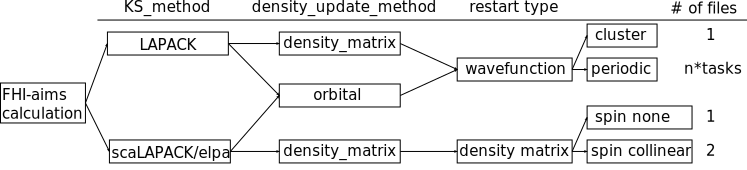
\includegraphics[width=0.9\textwidth]{./imgs/restart_scheme}
  \caption{Scheme of different restart types depending on used methods.}
  \label{fig:restart_scheme}
\end{figure}

For technical reasons there is not one single way, but the above mentioned
variants with again, variants.

The \emph{density matrix} based restart always
writes one file per spin-channel, no matter how many parallel MPI tasks are
used.
The \emph{wavefunction} based restart generally writes a single restart file
for all cluster calculations and one file per MPI-task for periodic
calculations. Due to this periodic calculations using the \emph{wavefunction}
restart need to be restarted with the same number of MPI-tasks.

\subsection{Mixing variants - the "force\_single\_restartfile" option}
For a subset of possible calculations the above described differences are not
valid and it is possible to restart different calculations using one type of
restart file. This is the case for all possible cluster calculations (using
either the LAPACK or scaLAPACK/elpa solver) and for periodic calculations with
only 1 k-point, $\Gamma$-only (using either the LAPACK or scaLAPACK/elpa solver).

This is implemented via the keyword \keyword{force\_single\_restartfile}. Using
this functionality, it is for example possible to profit from the parallel ELPA
solver for huge systems and still get a file containing the KS-wavefunction for
post-processing.

\subsection{Comments on the 'restart' starting point and on self-consistency}
As noted in the description of the \keyword{restart} keyword, 
it is important to note that the \keyword{restart} infrastructure
corresponds to a restart from the last Kohn-Sham orbitals, not from
the last density. 

In practice, this means that the code will restart
from the last \emph{unmixed} Kohn-Sham density, not from the last
\emph{mixed} density. When restarting from a non-selfconsistent
starting point, this can lead to unexpected jumps in the calculated
non-selfconsistent total energy between the ``old'' and the ``new'' 
(restarted) FHI-aims run.

Only the self-consistent total energy is truly meaningful. This quantity (the
self-consistent) total energy should be the same for the same
stationary density, when approached from different starting densities.
However, note additionally that some systems may exhibit several
different self-consistent stationary densities even for 
the exact same atomic positions and for the exact same density functional. 
A simple example are
antiferromagnetic vs. ferromagnetic spin states in some systems. In
such cases, the true ground state in a DFT sense is the stationary density 
that yields the lowest energy. It can be found by way of a global search for
different stationary densities, usually by varying the initial density guess.


\subsection{Rotating the FHI-aims wavefunction}
\emph{This feature is new and tested for the case of weakly interacting organic
        molecules as can be found in organic crystals. If you encounter any
        problems or strange behaviour, please let us know!}

In many molecular systems a rotation does not change the electron density
(or wavefunction) of a system. Therefore, the same wavefunction can be used
again to restart such a calculaction.

This is especially true for weakly interacting systems such as van-der-Waals
bound organic crystals. In these cases, the wavefunction of each single molecule
in the crystals is not too different from the isolated wavefunction of a single
molecule. This can be exploited to start a FHI-aims calculation of huge
molecular systems from a \emph{superposition of molecular densities} instead of
the usual \emph{superposition of atomic densities}. 

This functionality is implemented as an external tool using Python and can be
found in the FHI-aims repository itself (Python-package \emph{aimsutils}) or at
\url{https://gitlab.lrz.de/theochem/aimsutils}.

If you use this functionality, please cite \emph{C. Schober, K. Reuter, H.
        Oberhofer, J. Chem. Phys., 144:054103, 2016}\cite{Schober2015}.

\subsubsection*{Important pre-requisites}
This functionality only works for restart files containing the wavefunction of
the system, not the density matrix. Therefore, please make sure you have
wavefunction restart files or use the option
\keyword{force\_single\_restartfile}. The FHI-aims output file of the
calculation is also necessary.

Rotations can be defined via Euler angles in \emph{zyz} convention or quaternions. 
To avoid any confusions with rotational conventions (especially with Euler
angles), the input geometry will be rotated and saved using the same rotation
matrix. Please be sure to check if your expected and the actual rotation are the
same (or directly use the generated \texttt{geometry.in}). 

The final rotated restart file is again in the wavefunction format.

\begin{verbatim}
- example_calc
|
+-- control.in              
+-- geometry.in             # necessary 
+-- aims.out                # necessary 
+-- restart.wavefunction    # name can be anything, will be parsed from outfile
\end{verbatim}

\subsubsection*{Examples}
The two examples are shown using pre-defined scripts, but it is
totally possibly to use the Python package directly. The full Python API is
available via the Sphinx-documentation of the \emph{aimsutils} package.

\paragraph{Rotation of a single system:} The script \texttt{RotateSingle.py} can be
used to create the rotated geometry and restart for a single calculation.
\begin{verbatim}
        $: # RotateSingle alpha beta gamma -t x y z
                          '-----.-----'    '---.---'
                          Euler angles   translation vector
        $: RotateSingle 45 0 123 5.4 2.3 6.3

        $: # RotateSingle x_i x_j x_k x_l -t x y z
                          '------.------' '---.---'
                            quaternion   translation vector
        $: RotateSingle 0.33 -0.12 0.44 0.84 5.4 2.3 6.3
\end{verbatim}
This will create a subfolder \emph{rotated} with the new \texttt{restart.combined}
and \texttt{geometry.in}.

\paragraph{Rotation and combination of wavefunctions} The script
\texttt{RotateMany.py} reads a instruction file (\texttt{rotations.in}) with the
following format:
\begin{verbatim}
            # Comments or empty lines are ignored

            # title will also be foldername
            title project_x
            # lattice vector for new cell if any
            lattice_vector 11.2 0.00 0.00
            lattice_vector 0.00 10.5 0.00
            lattice_vector 0.00 0.00 10.7
            # now all rotated molecules
            # Euler angles (zyz)
            # alpha beta gamma x y z parent_molecule
            33.4 12.4 167.0   10.  0.  0.  calc_2
             0.  45.    0.     3.5 2.1 5.4 calc_1
           130.  90.   23.     0.  2.6 12. calc_3
            # OR Quaternion
            # x_i x_j x_k  x_l   x y z
            -0.4 0.15 0.33 -0.84 4 0 0 calc_2
            -0.2 0.45 0.13  0.84 0 2 0 calc_1
             0.0 0.00 0.00 -0.32 4 4 5 calc_3
\end{verbatim}

The necessary converged FHI-aims calculations must be in subfolders with the
appropriate name:
\begin{verbatim}
- calc_something/ (main calculation folder)
|
+-- rotations.in
+-- calc1/
    |
    +-- ...
+-- calc2/
    |
    +-- ...
+-- calc3/
    |
    +-- ...

\end{verbatim}
This will create a subfolder \texttt{project\_x} with the rotated wavefunction
assembled from the individual calculations defined in the script
(\texttt{restart.combined}) and geometry (\texttt{geometry.in}).

\subsubsection*{Theory}
\label{Sec:rotated-restarts}
The following should give a summary of how the rotation of wavefunctions can be
done with FHI-aims. For details on the used methods and mathematics, please
have a look at the references.

In FHIaims, a basis function is defined as
\begin{align}
    \Phi_{i,lm} = \frac{u_i(r)}{r}\cdot S_{l,m}(\theta, \phi),
\end{align}
with $S_{l,m}(\theta, \phi)$ being real valued spherical harmonics. These are
obtained from the complex spherical harmonics $Y_{lm}$ via
\begin{align}
        S_{l,m}(\theta, \phi) = 
    \begin{cases} 
            \frac{(-1)^m}{\sqrt(2)}(Y_{lm} + Y_{lm}^*) & m > 0\\
            Y_{l0} & m=0\\
            \frac{(-1)^m}{i\sqrt(2)}(Y_{l|m|} - Y_{l|m|}^*) & m < 0\\
    \end{cases}
\end{align}
A wavefunction is then given by
\begin{align}
        \Psi_k(r) = \sum_{i=1}^{\text{n\_basis}}c_i^k\Phi_i(r)
\end{align}
with the coefficients $c_i^k$. 

A rotation of the molecule (rotation matrix $\mathbf{R}$ leads to the same set
of YLMs $\mathcal{Y}$ (as they are fixed with respect to the xyz-coordinate
system), but with different coefficients $\mathbf{c}$ (new linear combination
of basis functions):

\begin{align}
    \mathbf{c'} = \mathbf{R}\mathbf{c}
\end{align}

The rotation of complex YLMs can be done with Wigner~D matrices ($D^l_{mm'}$).
For real YLMs different schemes are
available\cite{lessig_efficient_2012,aubert_alternative_2013,blanco_evaluation_1997}.
Due to the non-default YLM convention in FHIaims we construct our rotation
matrices for different $l$ from the complex Wigner~D matrices via the
transformation matrix $\mathbf{C}^l$ (reference:
\cite{blanco_evaluation_1997}):
\begin{align}
        S_{l,m} = \mathbf{C^l}Y_{l,m}
\end{align}
The matrix $\mathbf{C}$ is constructed according to
\cite{blanco_evaluation_1997} with the constraint of the different sign
convention in FHIaims. The real rotation matrix $\Delta^l(R)$,
\begin{align}
        \Delta^l(R) = \left(\mathbf{C}^l\right)^*\mathbf{D}^l(R)\left(\mathbf{C}^l\right)^t,
\end{align}
is then used to obtain the rotated coefficients for each $l, m$ for each basis
function in the system.
\begin{align}
    \mathbf{c}'^{l} = \Delta^l(R)\mathbf{c}^{l}
\end{align}


%\include{appendix_ASENEB}
% My own linked keywords definitions
% So I don't pollute the entire doc with tons of keywords
% These won't be added to the index
\newcommand{\chainkey}[1]
{\hyperlink{aimsChain#1}{\texttt{#1}}}

\newcommand{\chainkeydef}[2]
{

\centerline{\rule{1.0\textwidth}{1pt}}
\hypertarget{aimsChain#1}{\textbf{Tag: \texttt{#1}}{ \color{filename_color} (chain.in)}}
%\index{#1@\texttt{#1}}
\\[2ex] \hspace*{0.05\textwidth}
\begin{minipage}{0.92\textwidth}
  #2
\end{minipage} \\

\vspace{1pt}
}


\section{Finding Transition States: the aimsChain}
This project aims to provide an all-in-one package for various flavours of the chain of states methods for finding the minimum energy path(MEP). Currently the nudged elastic band method (NEB)\cite{NEBORI,NEBTAN}, the string method\cite{STRORI}, and the growing string method\cite{GSMoriginal} are included. 

Please direct any questions or suggestions to \textit{yaoyingyu@hotmail.com}, we need your help to improve the package.

\emph{The aimsChain code is distributed under the Lesser General
  Public License as published in Version 3, 29 June 2007, at
  http://www.gnu.org/licenses/lgpl.html . Some of the optimizer
  routines in the code originated within the Atomic Simulation
  Environment (ASE). We wish to give full credit to the developers of
  these routines. The aimsChain code can also be found in a separate
  distribution maintained by Yingyu Yao. The reason we distribute them
  directly within the FHI-aims repository is for the convenience of
  all FHI-aims users, but again: We wish to give full credit to the
  work and the license of the original authors within ASE.}

\subsection{Installation}
The package is located in \texttt{src/aimsChain}. 

In general, any computer/cluster that is capable of running FHI-ams and has numpy/scipy support can be used. 
To install, user should follow these simple steps:
\begin{enumerate}
\item Copy the package to the directory where you normally install softwares, e.g. \texttt{\textasciitilde /local/bin} or your home directory.
\item Modify your \texttt{\textasciitilde/.bashrc} to include the following lines 
\begin{verbatim}
 export PATH=$PATH:<package path>/tools
 export PYTHONPATH=$PYTHONPATH:<package path>
 module load python/scipy/2012.10
\end{verbatim}
These modifications are recommended but not necessary. You can also add them to your job script instead if you do not want to pollute your \texttt{.bashrc}.

The last line serves to load scipy into your system. On clusters you can normally find the corresponding keyword using \texttt{module avail}, and this could also be done by including \texttt{scipy} and \texttt{numpy} in your \texttt{\$PYTHONPATH}. 

Although unlikely, future updates of numpy/scipy may cause compatibility issues. If you observe anything strange in this regards, please let me know. 
\item You are done.
\end{enumerate}
To test your installation, source the \texttt{.bashrc} file and start a python shell. The package is successfully linked if executing
\begin{verbatim}
import aimsChain
import scipy
import numpy
\end{verbatim}
reports no error. Otherwise please double check your configurations and search for installation problems. 	

\subsection{A Quick Start}
While offering an extensive list of keywords, the package is aimed to work with most systems out of the box. Often very little configuration is required to conduct a successful path search. The keywords are available, on the other hand, to make the package as adjustable as possible, so that it can be finely tuned to tackle the less conventional systems. 

In the package directory, a few sample jobs have been prepared, imitating several different possible use cases. Please modify \texttt{chain.in} in each sample (other than sample 1) so that \chainkey{run\_aims} links to your own aims executable.
\begin{itemize}

 \item sample 1: This is a graphical example on a 2D analytic surface that demonstrates the principles behind the chain-of-states methods. You can skip it if you have used NEB/SM elsewhere. 
 
 You can and should run this demo in your personal computer instead of the cluster, since it is not actually calling FHI-aims for calculations.

 To start, you should go to \texttt{samples/sample1/run} and execute \texttt{job.sh}. This will execute the MEP finding algorithm on the 2D LEPS potential energy surface. To see the resulting process, proceed to \texttt{samples/sample1} and run \texttt{gnuplot plot.gnu} to see the evolving path on the surface. 
 
 This is also the perfect test bench for testing with different configurations. However keep in mind that performance in 2D is very different from the 3N-D space in reality, and therefore this example should not be used for performance optimization.
 \item sample 2: The inversion of an ammonia molecule. This example surveys the MEP with 8 images, using an very tight convergence setting(\chainkey{force\_thres}=0.01), which is too tight for most of the more complex systems, and will require tremendous amount of computation for non trivial systems in general. The resulting path would represent a very accurate representation of the MEP. 
 \item sample 3: This example measures the energy barrier to transfer a methyl group from one chlorine atom to another. It is using 6 images, coupled with a relatively loose convergence setting(\chainkey{force\_thres}=0.2). The resulting MEP from this is in general not accurate enough for a quantitative analysis. However, \hyperlink{aimsChainuse\_climb}{climbing image} is turned on with a relatively tight convergence setting(\chainkey{climb\_thres}=0.05). The result is an accurate energy barrier calculation. 
 
 Note that in this example we are also utilizing \keyword{constrain\_relaxation} in our input geometries to limit the movement of atoms. In this particular case, one of the chlorine atom is fixed at the origin, and the others are constrained to move along the x-axis. 
 \item sample 4: In this example we demonstrate how to start from an \hyperlink{aimsChainexternal\_geometry}{external set of initialization images}. We are calculating the MEP for a non-trivial isomerization. Geometries from an previous calculation is provided as the starting geometries. 
 \item sample 5: This sample provides an insight into MEP searching with periodic systems. It involves only the \texttt{interpchain.py} provided in \texttt{aimsChain/tools}, which should be already in your \$PATH if you followed the installation process. This tool will generate an initial path exactly the same way as the actual job script does. The result is printed into a directory named
 \texttt{interpolation}. A multi-frame \textit{.xyz} file is written, as well as one \textit{.in} geometry file for each image. 

Sample 5.1 and 5.2 are the same geometry, the only difference is that \hyperlink{aimsChainperiodic\_interpolation}{periodic interpolation} is set to \texttt{true} in the former, and \texttt{false} in the latter. Run \texttt{interpchain.py} in each directory and inspect the resulting path with your favourite visualization software. In sample 5.1 we acquire a smooth interpolation, but in sample 5.2 with periodic interpolation turned off, one row of atoms had to travel across the entire cluster. 

Another way to do a correct interpolation is shown in sample 5.3. You can manually adjust the coordinate of the atoms so that they are set at the correct coordinate with respect to the initial geometry. \texttt{fin.in} is adjusted in this case to reflect the change. This way, the interpolated path is again correct, even though \chainkey{periodic\_interpolation} is turned off. This is the preferred method of dealing with periodic systems, because the automatic interpolation finds the shortest path, but not necessarily the correct path. When working with periodic systems you should always do a \texttt{interpchain.py} first and inspect the result before running the actual job. 
\item sample 6: Here we show when and why the growing string(GSM) method should be used. Here the isomerization process involves rotation of in dihedral angles, and linear interpolations would result in overlapping atoms, which can be checked using the \texttt{interpchain} tool. 

The traditional approach dealing with these cases is to rotate the atoms manually and generate a non-overlapping initial path. GSM provides an alternative to this approach by growing the string from end points, which eliminates the need for manually generated initial path. 
\item sample hydra: It is essentially the same as sample 1, but prepared for the hydra cluster. This demonstrates the required modifications when transferring between different platforms.  
\end{itemize}

The samples include the following files. 
\begin{itemize}
 \item ini.in: initial geometry in the standard aims format
 \item fin.in: final geometry in the standard aims format
 \item control.in: standard control file for aims. This control will be used for all aims calculations.
 \item job.sge: job submission script, which you submit into the cluster. 
 \item chain.in: control file for aimsChain, see below for a detailed description
\end{itemize}
If everything is set up properly, you can simply \texttt{qsub job.sge} to get the job running. When running on clusters not using SGE, the job scripts must be changed accordingly. 

\subsection{Configuration}
\subsubsection*{aimsChain control file}
The chain control file is the file that governs the evaluation of MEP. It follows the same configuration convention set by the aims \texttt{control.in}, namely a list of key value pairs. The control file should be named \texttt{chain.in}.

This is a sample control file.

\begin{verbatim}
#A sample chain.in
run_aims mpiexec -ppn 8 -n $NSLOTS ~/bin/aims.062812.scalapack.mpi.x
initial_file ini.in
final_file fin.in
n_images 6
force_thres 0.2
use_climb true
climb_thres 0.05
\end{verbatim}

All the available keywords for the control are listed below:

\chainkeydef{run\_aims}
{
Usage: \chainkey{run\_aims} your command

Purpose: Provide the command that is used to call aims in your environment. 

Default value: mpiexec -ppn 8 -n \$NSLOTS \textasciitilde/bin/aims.081912.scalapack.mpi.x
}
You will need to change the default value for whatever command you are using.

There is no need to quote your command, simply type it as you would in
a bash shell. Everything after the keyword are concatenated into a single
string. 


\chainkeydef{initial\_file}
{
Usage: \chainkey{initial\_file} filename


Purpose: Provide the initial geometry file for the path. 


Default value: ini.in
}
The format should be the same as the aims \texttt{geometry.in}. Flags such as constraints are interpreted, and will affect the evaluation of MEP. All the intermediate images will have the same constraints as the initial geometry. 

Atoms in the initial and final geometry must establish a one to one correspondence. The $i$th line in the initial geometry and the final geometry must correspond to the same atom. Often there are many possible combinations, it is the user's responsibility to use the most physical one and/or check different combinations. You can perform a test interpolation with the \texttt{interpchain.py} tool provided. 

\chainkeydef{final\_file}
{
Usage: \chainkey{final\_file} filename


Purpose: The final geometry for the path. Refer to \chainkey{initial\_file}.


Default value: fin.in
}

\chainkeydef{n\_images}
{
Usage: \chainkey{n\_images} value


Purpose: The number of images used for MEP calculation.


Default value: 5
}
 Suitable value for this variable is highly dependent on the desired degree of resolution and the complexity of the system. A simple single barrier reaction will require 5 images to achieve a good result, while more complex potential energy surfaces require roughly 3 or more images per hill/trough. 
 
 
 If the geometry is not computationally expensive(tens of seconds per calculation with a reasonable \# of CPUs), the simple principle of ``the more the merrier'' can always be applied. 
 
 \chainkeydef{external\_geometry}
{
Usage: \chainkey{external\_geometry} file\_name


Purpose: If this variable is set, the initial set of images will be obtained from a external source instead of a linear interpolation.

Default value: None
}
 This flag should be set to the filename of a text file listing all of the intermediate geometries in order, e.g.
\begin{verbatim}
./geo/1.in
./geo/2.in
./geo/3.in
\end{verbatim}
It is advised that if you have anything better than a direct linear interpolation, you should use it as the initial guess. Linear interpolation can be highly inefficient, and would result in cases which never converges. When in doubt, you can always use the growing string method. 

\chainkeydef{periodic\_interpolation}
{
Usage: \chainkey{periodic\_interpolation} true/false


Purpose: Whether or not interpolation is done while considering periodic boundary.

Default value: False
}
This setting affects periodic systems only. If set to true, each atom's final geometry will be checked against all periodic counterparts to find the shortest path between the initial and final geometry. This can resolve some problems caused by the periodic boundary condition. Consult sample 4 for detailed usage. Always use the provided \texttt{interpchain.py} tool to check the resulting interpolation and confirm that it's physical before running. 

\chainkeydef{resample}
{
Usage: \chainkey{resample} true/false 


Purpose: Resample the input path into arbitrary number of images. 

Default value: False
}
This tag is effective only when \chainkey{external\_geometry} is set. When \chainkey{resample} is set to true, the package will resample the path you provided and interpolate it to have \# of images equal to \chainkey{n\_images}. This can be very useful if you find your calculation to have an inadequate number of images. You can extract the geometries from the final iteration, and start a new job by resampling them. 

\chainkeydef{aims\_restart}
{
Usage: \chainkey{aims\_restart} value 


Purpose: Reuse the wave function restart file to speed up the calculation. This should set to be the same as \keyword{restart} in \texttt{control.in}.

\textbf{WARNING!} This function is not compatible with aims as of July 2013, and only works occasionally.  


Default value: None
}
Value should be the same as \keyword{restart} in your \texttt{control.in}. The wave function restart file will be copied from iteration to the next, so that the scf cycles can start from an existing configuration. When working correctly, this can cut the computation time required by half or more. 

However, at this stage \keyword{restart} has very limited check on the input restart file, resulting in an error when the wave functions don't match. Do not use this keyword unless you are sure that your version of aims will start a new scf initialization instead of reporting errors when the wrong restart file is provided. If certain of which, however, the keyword should always be used to speed up the calculation. 

Setting \keyword{restart} will consume a decent amount of disk space. You may want to remove the restart files if you are planning to store the calculation permanently.


\chainkeydef{restart}
{
Usage: \chainkey{restart} true/false


Purpose: Whether the package will allow restarts. When set to true, you can simply submit the job again to continue from the previous calculations. 

Default value: true
}
When set to true, a restart file will be written as the path iterates. When the job is submitted/resubmitted, it will first check for the restart file to see if it's possible to start from a previous calculation. This is useful, when, for example, your job is killed due to time limitations on the cluster. Please refrain from changing settings between restarts, which is always error prone. If you are planning to change some settings, it's always safer to extract the most recent geometries and use them as the initial path for a new calculation. 

There is still the risk that the job is killed while the restart file is been written, in which case anything could happen when the job is resumed. However, considering the rarity of such event, it should not be a problem in practice.  

\chainkeydef{method}
{
Usage: \chainkey{method} neb/string


Purpose: Pick the method to use for the MEP calculation. 


Default value: string
}
Currently only string method and NEB are supported. In our testing, string method have shown to be slightly more stable than NEB, and therefore is our recommended method. 
\chainkeydef{neb\_spring\_constant}
{
Usage: \chainkey{neb\_spring\_constant} value 


Purpose: This sets the spring constant used in NEB calculation, and has no effect if \chainkey{method} is string. 

Default value: 20.0
}
It should be set to have the same magnitude as the force felt by the geometry, which is hard to determine before hand. However a generic value of 20 is good in general. Please try \chainkey{method} string first if you suspect that the spring constant have to be changed for the system to converge. 

\chainkeydef{force\_thres}
{
Usage: \chainkey{force\_thres} value


Purpose: The threshold for convergence. 

Default value: 0.2
}
Optimization will stop when the residual forces in the system is smaller than this preset value. If \chainkey{use\_climb} is true, climbing-image calculation will start after this threshold has reached. $0.2eV$ is always a good starting point, and for more rigorous calculations $0.1eV$ or $0.05eV$ can be used. Do not set it too small, since some numerical noises in the forces will always exist even when the path is well converged.  

Also note that adequate value is dependent on the system. A reaction with a $3 eV$ barrier can be much more well converged at $0.05 eV$ threshold than a reaction with a $0.3 eV$ barrier at the same threshold, because the former, very often, has a steeper barrier and hence larger force by nature. 

\chainkeydef{optimizer}
{
Usage: \chainkey{optimizer} dampedBFGS/BFGS/LBFGS/trm/CG/FIRE


Purpose: This picks the optimizer used for optimization. 

Default value: dampedBFGS
}


\textit{BFGS} is a textbook implementation of BFGS optimizer, which was observed to have wild behaviour is some situations. The fact that BFGS series of optimizer can be used for this type of calculations is in fact purely coincidental. The series of force projections involved in the chain of states methods can severely hamper the effectiveness of quasi-Newton optimizers. Please resort to FIRE optimizer whenever you observe wild behaviour in the optimization process. 


\textit{dampedBFGS} damps the original BFGS optimizer using several techniques, and is slightly more stable in those situations. (But they still get stuck from time to time!) This is the default setting that should always be tried first.


\textit{LBFGS} is the limited memory version of BFGS, which uses less memory for extremely large systems. However, given that in general FHI-aims is applied to systems with hundreds of atoms at most, this optimizer has little advantage in this front. However, due the fact that LBFGS uses only recent iterations for approximation, the results can be quite different from BFGS in a some PES. Therefore it's worth trying if BFGS fails.

\textit{trm} is the same trust-radius method ported from FHI-aims. In our tests it has proven to be reasonably stable and efficient. We would recommend this as another alternative along with FIRE when dampedBFGS fails.

\textit{CG} is the textbook implementation of conjugate-gradient algorithm using finite difference scheme. In our tests it has not shown any advantage over other algorithms, ans is provided for the sake of completeness. 

\textit{FIRE} is the Fast Inertial Relaxation Engine, one of the better non-Newton type optimizers. It is slower than BFGS series of optimizers in general, but is immune to the aforementioned instability because it does not approximate the Hessian. If dampedBFGS fails, try FIRE with \chainkey{global\_optimizer} off as an alternative. 

\chainkeydef{global\_optimizer}
{
Usage: \chainkey{global\_optimizer} true/false


Purpose: Whether all images are optimized as a single object, or if individual images are optimized as separated object. 


Default value: true
}
The global version, when coupled with BFGS-series of optimizer, is often faster than the non-global optimizer. However, this combination is less stable, and can lead to wild results. The non-global optimizer coupled with FIRE seems to be the most stable one in our tests, but is much slower than the former. Non-global optimizer combined with BFGS, on the other hand, slows the calculation significantly due to overestimation, and should be avoided. 

\chainkeydef{xyz\_lattice}
{
Usage: \chainkey{xyz\_lattice} a b c


Purpose: This key only affects the \textit{.xyz} file written in \texttt{paths} directory. It governs how the lattice is repeated in each lattice vector. The default is a standard 2 2 1 setting, valid for most surfaces. 

It has no effect on clusters. 


Default value: 2 2 1
}

\chainkeydef{map\_unit\_cell}
{
Usage: \chainkey{map\_unit\_cell} true/false


Purpose: This key only affects the \textit{.in} file written in \texttt{paths} directory. It determines whether atoms in these geometries are mapped back to the central unit cell. 

It has no effect on clusters

Default value: false
}


\chainkeydef{use\_climb}
{
Usage: \chainkey{use\_climb} true/false


Purpose: This will turn on the climbing image\cite{HenkelmanJCP2000a} feature. 


Default value: false
}
The points with highest energies will move toward a higher energy location along the path until the saddle point is reached. Please consult \chainkey{climb\_mode} for a detailed explanation of this process. If you are only interested in finding the energy barrier, it's possible to set \chainkey{force\_thres} to some larger value, such as 0.2, and set \chainkey{climb\_thres} smaller(e.g. 0.05) for a reasonably tight convergence. In this case decreasing \chainkey{force\_thres} will not affect the accuracy of climbing image, so long as the climbing image converges. Transition state finding can be sped up significantly this way by reducing the number of single point calculations required. 

\chainkeydef{climb\_thres}
{
Usage: \chainkey{climb\_thres} value


Purpose: Set the convergence criterion for the climbing image. 

Default value: same as \chainkey{force\_thres}
}
The climbing image will stop when the residual forces in the system is smaller than this value. It is normally, although not necessarily, set to a value smaller or equal to \chainkey{force\_thres}. In simple systems, the climbing image is capable of pushing the system done to $meV/\AA^{2}$ range, but that's not as plausible in larger systems.



\chainkeydef{interpolated\_climb}
{
Usage: \chainkey{interpolated\_climb} true/false


Purpose: Determine whether the climbing image is chosen from one of the existing images or interpolated from known energies and geometries. 


Default value: true
}

When set to true, the current energies and geometries will be fitted with a cubic spline to identify the point with highest energy. If this geometry is sufficiently far from existing nodes, then the interpolated geometry is used. If the geometry is close to one of the existing images, than that image is set to be the climbing image. 

When set to false, the image with highest energy is set to be the climbing image. 


\chainkeydef{climb\_mode}{
Usage: \chainkey{climb\_mode} 1/2/3


Purpose: This determines the ``mode'' of the climbing image. 

Default value: 2
}
Increasing mode corresponds to increasing stability and decreasing efficiency. The main difference lies in the number of images that are allowed to move during the climbing process. 


\chainkey{climb\_mode} 1: Only the image with highest energy is allowed to move. This setting can manage many circumstances, provided that \chainkey{force\_thres} is small enough so that the converged path provides a stable basin. 



\chainkey{climb\_mode} 2: The image with highest energy and its two neighbouring  images are allowed to move. The two additional image provides an evolving tangent estimate as the central image climbs. This mode can tackle nearly all cases where \chainkey{climb\_mode} 1 fails under the same \chainkey{force\_thres} setting. It is safe, in general, to set \chainkey{force\_thres} to 0.3 if you are only interested in energy barrier. 


\chainkey{climb\_mode} 3: All of the images excluding the end points are allowed to move. This is the most stable, but rarely necessary setting. The efficiency drop is highly dependent on the system and the \chainkey{force\_thres} setting. In general this should be used as a last resort when \chainkey{force\_thres} can be converged to a tight setting but climbing image on other modes fails. 






\chainkeydef{climb\_global\_optimizer}
{
Usage: \chainkey{climb\_global\_optimizer} true/false


Purpose: The same as \chainkey{global\_optimizer}, except this keyword is dedicated for climbing image. 

Default value: true
}
The tag has no effect when \chainkey{climb\_mode} is 1, in which case the global and non-global optimizer are equivalent. Unlike \chainkey{global\_optimizer}, BFGS+Non-global setting can be a good combination for \chainkey{climb\_mode} 2 if the default setting fails, mainly due to the well behaving local basin for a roughly converged string. 



\chainkeydef{climb\_optimizer}
{
Usage: \chainkey{climb\_optimizer} dampedBFGS/BFGS/LBFGS/CG/TRM/FIRE 


Purpose: The same as \chainkey{optimizer}, but dedicated for climbing image.


Default value: fire
}


\chainkeydef{climb\_control}
{
Usage: \chainkey{climb\_control} file\_name


Purpose: Specify a different \texttt{control.in} for the climbing image. 

Default value: control.in
}
It's possible, for example, to converge the entire path with a light setting, and then converge the climbing image with tight setting, which consumes far less computational power. 

However, there are a few things to note if this feature is utilized. First, \chainkey{force\_thres} must be set smaller than normal, perhaps even the same value as \chainkey{climb\_thres}. Since a different control file can produce a radically different PES, you would like to be as accurate as possible when converging the string, so that the error is not amplified with a tighter setting. Secondly, it's better to use \chainkey{climb\_mode} 2 or 3 for these kind of computations, since the single image climbing mode can rarely recover from a bad starting point. 

This feature is best suitable for production works where a tighter setting which will dramatically increase the time required for single point calculations.

As an alternative, you can also kill your running process and change the \texttt{control.in} file manually before restarting the process. 


\chainkeydef{use\_gs\_method}
{
Usage: \chainkey{use\_gs\_method} true/false 


Purpose: This controls whether the growing string method is used or not. 


Default value: False
}
The growing string method(GSM) is explained in sample 6. It is best suitable for cases where it is certain that linear interpolations between initial and final images will not lead to a correct path. This can be caused by movements such as rotations. It is also useful when doing large-scale automated scanning, where the user does not have the time to look at geometries on a case by case basis.

When set to true, the path will start from the two end point and slowly grow inward to generate a physical path. When the path is completely grown, it will be passed onto NEB/SM for further calculations.

Beware that when direct interpolation can lead to correct paths, e.g. surface dispersion, using growing string method may reduce efficiency. 

\chainkeydef{gs\_thres}
{
Usage: \chainkey{gs\_thres} true/false 


Purpose: The GSM counterpart for \chainkey{force\_thres}.


Default value: \chainkey{force\_thres}*1.5
}

When the forces in the system goes below this preset value, a new node will be added to the path. It should not be set too small, since the purpose of GSM is to generate a physical path, not a well-converged path. The default value gives a good guideline for this key. 


\chainkeydef{gs\_n\_images}
{
Usage: \chainkey{gs\_n\_images} value 


Purpose: The GSM counterpart for \chainkey{n\_images}.


Default value: \chainkey{n\_images}
}

In some circumstances, you may want to specify a different number of images for the growing stage of the calculation. This key serves this purpose. After the growing process, the path will be re-sampled to match the value of \chainkey{n\_images}

\chainkeydef{gs\_optimizer}
{
Usage: \chainkey{gs\_optimizer} dampedBFGS/BFGS/LBFGS/trm/CG/FIRE 


Purpose: The GSM counterpart for \chainkey{optimizer}.


Default value: trm
}

For GSM, dampedBFGS, trm, and FIRE are optimizers worth trying. 

\chainkeydef{gs\_global\_optimizer}
{
Usage: \chainkey{gs\_global\_optimizer} true/false


Purpose: The GSM counterpart for \chainkey{global\_optimizer}.


Default value: false
}

We have not done enough testings to determine conclusively the better set of optimizers. The default provided here have performed well in our benchmarks, but feel free to try other combinations.

\chainkeydef{lbfgs\_alpha}
{
Usage: \chainkey{lbfgs\_alpha} value


Purpose: Set the curvature used to initialize the Hessian(in $eV/\AA^{2}$) in LBFGS. In general any value that is not magnitudes off are acceptable. 


Default value: 120.0
}

\chainkeydef{lbfgs\_memory}
{
Usage: \chainkey{lbfgs\_memory} value


Purpose: Set the number of past iteration that LBFGS is going to remember. A larger value will increase memory consumption, and a small value will decrease accuracy.


Default value: 30
}

\chainkeydef{lbfgs\_maxstep}
{
Usage: \chainkey{lbfgs\_maxstep} value


Purpose: The maximum step in $\AA$ that an atom can take in a single iteration. This is similar to \keyword{max\_atomic\_move}, but defaulted to a much smaller value due to the increasing complexity.


Default value: 0.04
}

\chainkeydef{bfgs\_alpha}
{
Usage: \chainkey{bfgs\_alpha} value


Purpose: Same as \chainkey{lbfgs\_alpha}, but used by BFGS, trm, and dampedBFGS optimizers.


Default value: 120
}

\chainkeydef{bfgs\_maxstep}
{
Usage: \chainkey{bfgs\_maxstep} value


Purpose: Same as \chainkey{lbfgs\_maxstep}, but used for BFGS and dampedBFGS optimizers.


Default value: 0.04
}

\chainkeydef{fire\_dt}
{
Usage: \chainkey{fire\_dt} value


Purpose: The initial time step used by the FIRE optimizer. 

Default value: 0.02
}
It is set to a very conservative value because FIRE is intended to be used as a fall back when BFGS fails. Values up to 0.1 can be used to speed up the calculation, provided that the PES is smooth enough. Internally, the time step is dynamically adjusted, and this key only serves to initialize the value. 

\chainkeydef{fire\_maxstep}
{
Usage: \chainkey{fire\_maxstep} value


Purpose: Same as \chainkey{lbfgs\_maxstep}, but used for FIRE optimizer.


Default value: 0.04
}

\subsection{Preparation before running}
\subsubsection*{Creating a project directory}
You should create a directory for each and every aimsChain calculation you are planning to run. It should contain the following files.
\begin{verbatim}
 -Project directory
 |
 |--chain.in
 |
 |--control.in
 |
 |--ini.in*
 |
 |--fin.in*
 |
 |--extgeo.lst*+
 |
 |--images*+
      |
      |-image1.in*+
      |
      |-image2.in*+
      |
      |-... 
*The filename can be set by the user
+The files are only necessary for starting from external geometry. 
\end{verbatim}

\subsubsection*{geometry file}
The initial and final geometry should be in the standard aims input format. Keywords such as constraints will be interpreted. The \keyword{constrain\_relaxation} tag should be used with caution--it acts as a double-edged sword in terms of MEP evaluation. You can try to remove the constraint tag from sample 2 and observe the efficiency boost for example. In other cases, setting it may help convergence by reducing degree of freedoms.  

In addition, you should pre-align your initial and final geometries to remove any rotational/translational component in the geometry, this will reduce the computational effort required. 

The ordering of atoms in the geometry file is very crucial. The atoms in the initial and final geometry must establish a one to one correspondence, so that the $i$th line in the initial and final geometry represents the same atom. Changing the order can change the result from the evaluation dramatically. 

For example, consider the diffusion of benzene on a surface. By changing the ordering of atoms you may force the diffusion to be done via rotational or translational motion, which would result in very different MEP. If you can visualize more than one possible combination, try all of them to find the lowest barrier. It is a matter of fact that there often exists more than one MEP between two geometries, but the overall barrier is only determined by the MEP with lowest barrier. Chain of states methods will evolve toward the MEP that's closest to the initial path, but not necessarily the lowest in energy. 

\subsubsection*{aims control file}
The aims control file should contain two lines.
\begin{verbatim}
compute_forces .true.
final_forces_cleaned .true.
\end{verbatim}
This will turn on the force evaluation for aims, which is required for any chain of states method. 
\keyword{relativistic}, when required, must be set to \texttt{atomic\_zora scalar}, since we require force evaluations. 

Sometimes additional configurations can require more than the two lines listed above. For example, when using \texttt{b3lyp} you need to set 
\begin{verbatim}
RI_method lvl_fast 
\end{verbatim}
for a correct force evaluation. Generally you can find these information in the aims output. A rule of thumb is to relax the geometry using your configurations and skim through the aims output for any warnings. This will force aims to provide all warnings related to the calcualtion of forces. When you have confirmed that the configuration if warning-free, just comment out the \keyword{relax\_geometry} for aimsChain calculation.

You can also set \keyword{sc\_iter\_limit} to a lower value, which should still be much higher than the normal number of cycles that your system consumes. As the path evolves, it can be the case that during a few iterations the geometry become non-physical, and its scf cycle will never converge. Such cases often recover itself within a few iteration, and will not affect the final result. However, a default limit of 1000 will consume lots of computational power in these cases,  which is a complete waste especially for larger systems. 

The control file should not have \keyword{relax\_geometry}, any molecular dynamic keywords, and etc. The geometry should not be altered by aims.  
It is advised that you always use a light setting for the first run, so that tunning settings and confirming convergence can be done efficiently. If a more accurate result is desired, you can submit a tight run using the resulting geometries from the light run, which is always faster than a direct tight run from linear interpolation. 

To ensure efficiency, you should configure your control file so that each single point calculation takes at most few minutes to finish. If a tighter setting is desired, consider using \chainkey{climb\_control} for a different control file during climbing image. 
\subsubsection*{aimsChain control file}
It is unlikely that you will need a long list of keywords in your control. Tags should be added gradually if you find that the default settings is not sufficient for your purpose.
Keys that should be included on the first run are \chainkey{run\_aims}, \chainkey{initial\_file}, \chainkey{final\_file}, \chainkey{n\_image}, \chainkey{force\_thres}, \chainkey{restart}, and \chainkey{external\_geometry} if so desired. Simply grabbing the control from the samples will also work most of the times. 


If you believe that your system follows a rather straightforward path geometrically(i.e. diffusion, small rotation, etc.), you can set the climbing image on your first run and see if it works out correctly. For any complex paths, such as non-trivial isomerization, fine tunning of the control file can be required for the system to converge. 

\subsubsection*{job script}
The job script should contain a call to \texttt{runchain.py}, as well as loading the necessary modules if that is not done in \texttt{.bashrc}. No post processing should be included unless you are certain that the system will converge and terminate within the time limit.
 
\subsubsection*{external geometry}
If you have any information about the path you are trying to find, please include them here. This can be a guess for transition state, geometry reported by papers, or your own interpolation by tweaking atoms in a visualization software. Coupled with \chainkey{resample}, any number of external geometries can help speed up the calculation process, making the process very flexible. 

It is a common practice to take the intermediate path from a previous calculation (perhaps before it has gone wild) and use them as the initialization path for a new job. This is perfectly fine, and aimsChain outputs intermediate paths just for this purpose. However, when doing so please remember to remove the first and last image from the path, which are the same geometry as the initial and final states. The list of external geometries should only contain intermediate images, entering initial/final states in there will most likely lead to a dead end. 
 
\subsection*{growing string method}
GSM  offers another possibility for no-trivial calculations. If you believe your geometry will result in a geometrically complex reaction path, then using GSM will be your best bet. 

GSM works by starting from the two end point, and gradually adding images toward the centre of the path. Whenever an image is added, it will be evolved until its forces falls below a threshold. This way we are not requiring any a priori knowledge on the intermediate path, where the standard SM/NEB method approximates with a linear interpolation.

\subsubsection*{test the interpolation}
One of the most important step you can take to ensure a successful MEP evaluation is to ensure that the initial path is physical. This is especially true for periodic systems where the periodic boundary condition plays an unwanted part in this. 

We have provided a tool in \texttt{aimsChain/tools}, the \texttt{interpchain.py}. This gadget performs the resampling and interpolation process exactly the same way that the actual script is doing it, and therefore is a good way to check if the initial path is reasonable. 

When ran, the program will create the \texttt{interpolation} directory in your project directory (and will clear that folder if it already exists!). 
\begin{verbatim}
 -Project directory
 |
 |--interpolation
      |
      |-image001.in
      |
      |-image002.in
      |
      |-... 
      |
      |-path.xyz
\end{verbatim}

There will be \chainkey{n\_images}+2 aims geometry created, including initial and final geometry. A multi-frame \textit{.xyz} file is also created in the directory for use with visualization softwares that doesn't support multi-file animation. If the geometry is periodic, the \textit{.xyz} file is repeated in each lattice vector according to \chainkey{xyz\_lattice} to make visualization easier. (because the standard xyz does not encode periodic information) Always check the interpolation if you are working with a new project, which can save you lots and lots of time if you happen to spot a bad interpolation(as shown in sample 4).

\subsubsection*{a note on periodic systems}
Running aimsChain on periodic systems requires extra precaution, because initial files from a periodic system can often provide misleading initial path. 

The default interpolation algorithm when \chainkey{periodic\_interpolation} works as follows. For each atom in the final geometry, the coordinates are offset by each lattice vector in both the positive and negative direction. The results are compared with the same atom in the initial geometry, and the coordinate with the shortest distance is used as the actual coordinate for the final atom. This method is good in general. 

However, it's still possible to imagine cases where a longer path is the actual path. For example, when trying to simulate the effect of an edge on one end. The shortest path may corresponds to climbing over the edge to reach the other end, while the true path, moving in the other direction, is to simply walk away from the edge. 

In these cases, the coordinate of the final geometry must be adjusted manually, so that its coordinate corresponds to its true coordinate after the move, and does not involve any periodic boundary condition. \chainkey{periodic\_interpolation} should be turned off, and the interpolated path should be looked in details to ensure that the atoms in the base are also correctly interpolated. 

\subsection{Running the script}
When the script is running, it will first generate a few directories and files in the project directory. 

\begin{verbatim}
 -Project directory
 |
 |--forces.log
 |
 |--climbing_forces.log+
 |
 |--growing_forces.log*
 |
 |--iterations
 |    |
 |    |-iteration0000
 |    |    |
 |    |    |-aims-chain-node-0.00000
 |    |    |	|
 |    |    |	|-aims-chain-node-0.00000.out
 |    |    |	|
 |    |    |	|-control.in
 |    |    |	|
 |    |    |	|-geometry.in
 |    |    |
 |    |	   |-aims-chain-node-0.10000
 |    |	   |    |
 |    |    |    |-...
 |    |
 |    |-...
 |
 |--paths
      |
      |-iteration0000
      |    |
      |    |-image001.in
      |    |
      |    |-image002.in
      |    |
      |    |-...
      |    |
      |    |-path.xyz
      |    |
      |    |-ener.lst
      |    |
      |    |-path.lst
      |    
      |-iteration0001
      |    |
      |    |-...
      |    
      |-...
      
+only generated if climbing image is used
*only generated if growing string method is used
\end{verbatim}

\textbf{Warning!} Directories named \texttt{optimized}, \texttt{paths}, and \texttt{iterations} may be cleared/changed if they already exist. Don't leave useful information there!

The \texttt{iterations} directory is where all the aims single point calculations are done. Each iteration has its own directory, where each single point calculation is again put in its own directory. They are labelled by the unique id of the particular images as well as the iteration it is in. This is also the place where aimsChain stores optimizer and restart related files. 

The \texttt{paths} directory contains useful information for you while aimsChain is running. A directory is created for each iteration, containing all the necessary information you might be interested in. The \texttt{geometry.in} for each image is written, including the initial and final state. This is the perfect place to extract intermediate path if you would like to start a new job from there. Remember not to include the initial and final geometry in your external geometry list. A \textit{.xyz} animation is written, governed by \chainkey{xyz\_lattice}, which is handy for visualizing the current stage. \texttt{ener.lst} stores the current energy of the system, which is extracted from the aims outputs. The energies are offset so that the initial state is at the zero point. This will give a rough idea of the energy landscape along the path at the current iteration. \texttt{path.lst} lists the corresponding path in the \texttt{iterations} directory, in case you want to check the aims output for diagnostics.

\texttt{ener.lst} and \texttt{path.lst} also labels the state each image is in. A ``FIXED'' label indicates that the images is not been moved from iteration to the next, which can be the case for the initial and final geometry, as well as during climbing image calculation. A ``CLIMB'' label indicates that this image is the climbing image, and when converged, represents the geometry of the saddle point. Normal nodes are simply labelled ``Normal''.

There are also files named \texttt{forces.log}, \texttt{growing\_forces.log}, and \texttt{climbing\_forces.log} in your project directory, which records the residual forces in the system for each iteration. They are the most straightforward way to check the current state of the system. 

When the path is converged, the result will be put into a directory named \texttt{optimized}. They will have the same geometry as the last iteration in the \texttt{paths} directory, but they are copied from \texttt{iterations} directory so that the aims outputs are included. The same is down for growing string method. Once the growing process is completed all the relevant info are write to the \texttt{grownstring} directory, so you don't have to re-grow your geometries for different calculations. 

\subsection{Tips \& Guides On Running}
It is important to inspect the calculation once in a while when it's running, so that it can be stopped when going astray.


If the forces are going to extremely big values (several hundreds) after reaching a relatively small value, please have a look at the most recent geometry in \texttt{paths} to see if it's physical. Any non-physical path is most likely to have been caused by the BFGS optimizer. You should go backward and find the last iteration at which the geometries are physical (most likely corresponding to a small residual forces), and use that as the initial geometry for a new calculation with non-global FIRE optimizer or trm optimizer. 


If the forces goes up and down repeatedly, try switching off the global optimizer. If that doesn't help, try FIRE or trm. 


When climbing image is not converging, your \chainkey{force\_thres} might be too large for the system. If you are using \chainkey{climb\_mode} 1, consider extract the converged path before climbing started, and experiment with mode 2. Otherwise start a new calculation with the converged path and a higher threshold. 

If you are focusing on achieving a very precise calculation, and your system is not computationally intensive, you may want to do the following. Increase number of images used. Utilize \chainkey{climb\_control} for tighter convergence at climbing image. Use \chainkey{climb\_mode} 2 or 3 for climbing image. Start with non-global FIRE in the first place to avoid potential problems with BFGS.

If you are working with systems that are computationally expensive for aims, try these. Decrease the number of images, but use at least 3. (or more, if you have a complex reaction) First converge a path to a reasonable value.(below 1 $eV/\AA^{2}$ for example) Extract the path and try \chainkey{aims\_restart}. Your system may be one of the few that has a consistent wave function configuration as the string evolves to MEP. If the job stops after one iteration, then that has failed, simply re-submit the job after turning the flag off. Set \chainkey{restart} in both \texttt{control.in} and \texttt{chain.in}, even if you are not using \chainkey{aims\_restart}. This will save time when your calculation is stopped when exceeding the time limit. Try to use the lightest setting possible for the calculation. Only switch to tight settings after a good result is achieved on the light setting. 

When the climbing image is converged, the image that's labeled ``CLIMB'' in \texttt{ener.lst} is the transition state. It may be the case sometime that when using \chainkey{climb\_mode} 1, the converged transition state has a lower energy than its neighbour. This is not a problem in general, its neighbour was not well converged to the path. If you are worried about it, set a tighter convergence threshold or using a different climb mode will help. 


% some keywords occurring here are the same as in the original AIMS,
% their labels should not be doubly defined!
\newcommand{\doublekeydefinition}[3]
{{\textbf{Tag: \texttt{#1}}{ \color{filename_color} (#2)}}
#3

}
\section{Transition state search: Nudged Elastic Band method}
\label{appendix_NEB}

\emph{The functionality described in the present section is no longer
  the preferred option to calculate transition states in FHI-aims. We
  here keep it as legacy only. Please try the 'aimschain'
  functionality of the previous section first. Let us know if you
  are still using the old NEB.f90 version. Else, it will be removed in
  the near future.}

\subsection{Theory and methods}

\subsection{Usage}
The transition state search in AIMS at present is implemented in 
form of a PERL-script \option{NEB.pl} that calls a FORTRAN-90 code 
\option{NEB.f90}, both are located in the \option{src}-subdirectory
\option{NEB}. The Fortran code still has to be compiled with 
\option{LAPACK} and \option{BLAS} routines linked in. 

The job description of a TS-search is contained in a separate control 
file with a number of keywords defined below. That control file 
should be called \option{control\_NEB.in}. You may change the name
to anything else you like, just specify the name of the new control
file as an argument when calling \option{NEB.pl}. Note that (at present)
a lot of keywords are simply assumed to be there, and not enough 
testing is done to capture any missing options. This might lead to 
unexpected runtime behaviour. Please check to make sure everything 
you (think you) need is contained in the file \option{control\_NEB.in}.

The interface to this program is via multi-frame \option{xyz} geometry 
files, which are described under the keyword \keyword{input\_template}. 
You also need a control file template for the AIMS calls (see keyword 
\keyword{aims\_control\_file\_template}), which must contain a line of the 
form \\
\option{restart <}\keyword{aims\_restart\_string}\option{>} \\ 
where the restart file for the different images can be specified and 
passed on. Towards the end of a run, this functionality greatly
accelerates the DFT calculations. Also make sure that the AIMS 
control file template contains the two lines \\
\keyword{compute\_forces}  \option{.true.} \\
\keyword{final\_forces\_cleaned} \option{.true.}

The keywords used in the NEB-control file are:

\keydefinition{aims\_control\_file\_template}{control\_NEB.in}
{\begin{itemize}
  \item Usage: \keyword{aims\_control\_file\_template} \option{filename}
  \item Location of the AIMS template file to be used for the TS search.
  \end{itemize}}

\keydefinition{aims\_restart\_string}{control\_NEB.in}
{\begin{itemize}
  \item Usage: \keyword{aims\_restart\_string} \option{template\_string}
  \item Marker in the control file to be replaced by the actual restart file of a given iteration. 
  \end{itemize}}

\keydefinition{dft\_exe}{control\_NEB.in}
{\begin{itemize}
    \item Usage: \keyword{dft\_exe} \option{filename}
    \item \option{filename} is the AIMS executable including the full path.
  \end{itemize}}

\keydefinition{force\_convergence\_criterion}{control\_NEB.in}
{\begin{itemize}
    \item Usage: \keyword{force\_convergence\_criterion} \option{value}
    \item \option{value} is the convergence force component on any image coordinate 
                         after it has been corrected by the transition state search.
  \end{itemize}}

\keydefinition{input\_template}{control\_NEB.in}
{\begin{itemize}
    \item Usage: \keyword{input\_template} \option{filename}
    \item The location of the initial guess for the TS-search. The file name contains 
      the number of the iteration, followed by \option{.xyz}, while 
      \keyword{input\_template} should be without those two points. 
    \item Example: An initial guess called \option{space\_dog\_0.xyz} 
      would be described with \\
      \option{input\_template space\_dog\_}
    \item This file has to be a multi-frame xyz file with the following format:\\
      \option{<n\_atoms>} \\
      \option{start} \\
      \option{<species1> <xstart> <ystart> <zstart> }\\
      $\ldots$\\
      \option{<n\_atoms>}\\
      \option{image 1}\\
      \option{<species1> <x1> <y1> <z1> }\\
      $\ldots$\\
      \option{<n\_atoms>}\\
      \option{image <n\_images>}\\
      \option{<species1> <x1> <y1> <z1> }\\
      $\ldots$\\
      \option{<n\_atoms>}\\
      \option{END}\\
      \option{<species1> <x1> <y1> <z1> }\\
      $\ldots$\\      
  \end{itemize}}

\doublekeydefinition{max\_atomic\_move}{control\_NEB.in}
{\begin{itemize}
    \item Usage: \option{max\_atomic\_move} \option{value}
    \item The maximally allowed displacement during a single NEB step.
    \item This value should be relatively small (default is 0.1\AA) as the
      algorithm might literally tear apart some of the images if the 
      force constants are not set ideally and the transition path is not 
      extremely close to the actual path. 
    \item Same as keyword \keyword{max\_atomic\_move} in AIMS
  \end{itemize}}

\doublekeydefinition{line\_step\_reduce}{control\_NEB.in}
{\begin{itemize}
    \item Usage: \option{line\_step\_reduce} \option{value}
    \item for BFGS: factor by which a line step will be reduced if the 
      object function increased more than \keyword{object\_function\_tolerance}
      between two successive iterations. 
    \item at present only useful for \keyword{method} \option{PEB}, as there
      is no implementation of an object function for the other methods.
    \item This is the same as the original AIMS keyword \keyword{line\_step\_reduce}
  \end{itemize}}

\keydefinition{method}{control\_NEB.in}
{\begin{itemize}
    \item Usage: \keyword{method} \option{flag} \\
    \item \option{flag} can be either \option{PEB} or \option{NEB} for the pure 
      elastic band and the nudged elastic band methods respectively.
  \end{itemize}}

\doublekeydefinition{min\_line\_step}{control\_NEB.in}
{\begin{itemize}
    \item Usage: \option{min\_line\_step} \option{value}
    \item \option{value} is the minimal line step for the BFGS solver 
      below which the code simply executes a step in order to get out of 
      any numerical noise. 
    \item same as the keyword \keyword{min\_line\_step} in the original 
      AIMS code.
  \end{itemize}}

\keydefinition{n\_atoms}{control\_NEB.in}
{\begin{itemize}
    \item Usage: \keyword{n\_atoms} \option{value}
    \item \option{value} is the number of atoms in each image. 
\end{itemize}}

\keydefinition{n\_images}{control\_NEB.in}
{\begin{itemize}
    \item Usage: \keyword{n\_images} \option{value}
    \item \option{value} is the total number of images, not counting the start and end points. 
  \end{itemize}}

\keydefinition{n\_iteration\_start}{control\_NEB.in}
{\begin{itemize}
    \item Usage: \keyword{n\_iteration\_start} \option{value}
    \item Default \keyword{n\_iteration\_start} \option{= 0}
    \item If there is data available from a previous run of the same system,
      it might start at iteration \option{value} rather than from the beginning.
    \item Careful that you use the proper \keyword{save\_data} file if using this feature!
  \end{itemize}}

\keydefinition{n\_max\_iteration}{control\_NEB.in}
{\begin{itemize}
    \item Usage: \keyword{n\_max\_iteration} \option{value}
    \item \option{value} is the maximal number of iteration of the search.
  \end{itemize}}

\keydefinition{object\_function\_tolerance}{control\_NEB.in}
{\begin{itemize}
  \item Usage: \keyword{object\_function\_tolerance} \option{value}
  \item An iteration is rejected when the object function increases
    more than \option{value} between two successive iteration. 
  \item This only works for the pure elastic band \keyword{method}
    as there is no object function in the current NEB implementation.
  \item Same function as keyword \keyword{energy\_tolerance} in the main AIMS code.
\end{itemize}}

\keydefinition{save\_data}{control\_NEB.in}
{\begin{itemize}
    \item Usage: \keyword{save\_data} \option{filename}
    \item Gives a place to store BFGS and other information between successive iteration. 
    \item Be careful to delete this file when starting a new NEB run.
\end{itemize} }

\keydefinition{spring\_constant}{control\_NEB.in}
{\begin{itemize}
    \item Usage: \keyword{spring\_constant} \option{value}
    \item \option{value} is the single fixed spring constant throughout a single NEB run.
    \item Using this is either default or it should be done in conjunction with \\
      \keyword{use\_variable\_spring\_constants} \option{.false.}
  \end{itemize}}

\keydefinition{spring\_constant\_max}{control\_NEB.in}
{\begin{itemize}
    \item Usage: \keyword{spring\_constant\_max} \option{value}
    \item Maximal value in a range of possible spring constants
    \item can only be used together with the option \\
      \keyword{use\_variable\_spring\_constants} \option{.false.}
\end{itemize}}

\keydefinition{spring\_constant\_min}{control\_NEB.in}
{\begin{itemize}
    \item Usage: \keyword{spring\_constant\_min} \option{value}
    \item Minimal value in a range of possible spring constants
    \item can only be used together with the option \\
      \keyword{use\_variable\_spring\_constants} \option{.false.}
\end{itemize}}

\keydefinition{start\_BFGS}{control\_NEB.in}
{\begin{itemize}
    \item Usage: \keyword{start\_BFGS} \option{value}
    \item Force convergence criterion below which the algorithm switches
          from a steepest-descent type approach to BFGS algorithm. 
 \end{itemize}}

\keydefinition{switch\_to\_CI-NEB}{control\_NEB.in}
{\begin{itemize}
    \item Usage: \keyword{switch\_to\_CI-NEB} \option{value}
    \item will switch to using the climbing image nudged elastic band method
      after reaching a NEB force convergence of \option{value}
\end{itemize}}

\keydefinition{use\_variable\_spring\_constants}{control\_NEB.in}
{\begin{itemize}
    \item Usage: \keyword{use\_variable\_spring\_constants} \option{.true./.false.}
    \item If \option{.true.} a range of spring constants that depend linearly on the 
      energy \cite{HenkelmanJCP2000a} is used. 
    \item \option{.true.} Requires setting of the keywords \keyword{spring\_constant\_min} and 
      \keyword{spring\_constant\_max}
\end{itemize}}



\include{appendix_GA-2}
%\newcommand{\doublekeydefinition}[3]
% {{\textbf{Tag: \texttt{#1}}{ \color{filename_color} (#2)}}
% #3
% 
% }

\section{Plugin for free-energy calculations with molecular dynamics: \texttt{PLUMED}}
\label{appendix_PLUMED}


Molecular dynamics based free-energy calculations can be performed
with the aid of the external plugin \texttt{PLUMED}.\\
Methods included are metadynamics \cite{mtd}, well-tempered metadynamics \cite{wmtd}, umbrella sampling \cite{usa1,usa2,usa3}, Jarzynski-equation based steered molecular dynamics \cite{smd1,smd2}.
A large and nearly exhaustive set of collective variable (CV) is accessible through a simple input script.

\texttt{PLUMED} is a free package that, after registration, can be downloaded from 
\url{http://merlino.mi.infn.it/~plumed/PLUMED/Home.html}
Currently, a copy of the \texttt{PLUMED} library is
kept in the \emph{external} directory of the FHI-aims source code, and
must be compiled separately using the makefile Makefile.meta (see section
\ref{Sec:Makefiles}). In the future a patch for modifying FHI-aims in order to compile it with PLUMED will be available on the PLUMED webpage.\\

\subsection{Usage}

The actual use of the plugin is switched on by this single line in \texttt{control.in}:
\begin{verbatim}
 plumed .true.
\end{verbatim}
With \texttt{plumed .false.} (default) or nothing, the code would behave exactly as compiled without
this plugin. It is implied that some MD scheme must be used in \texttt{control.in}, in order to see PLUMED acting. What PLUMED does, in facts, is to modify the molecular dynamics forces according to the selected scheme.\\
All the specific controls of the free energy calculation are contained in the file \texttt{plumed.dat} (which must be in the working directory, together with \texttt{control.in} and \texttt{geometry.in}, if \texttt{plumed .true.} is set).
For all the details on \texttt{plumed.dat}, we defer to \texttt{PLUMED} manual which can be found on the project website.\\
Here we report a minimal example for metadynamics:
\begin{verbatim}
PRINT W_STRIDE 10
DISTANCE LIST 1 <g1> SIGMA 0.35
g1->
2 3 4
g1<-
HILLS HEIGHT 0.003 W_STRIDE 10
ENDMETA
\end{verbatim}
This script would make \texttt{PLUMED} deposit Gaussians (\texttt{HILLS}) of \texttt{HEIGHT} $0.003$ hartree, every \texttt{W\_STRIDE} timesteps.
The (only) CV that will be biased by metadynamics is a distance between atom `1' and the center of mass of atoms `2', `3', and `4'. The number labelling the atoms follows their order of appearance in \texttt{geometry.in}. The results will be printed (see below) every \texttt{PRINT W\_STRIDE} time steps.
The width of the Gaussian for the distance CV is specified by \texttt{SIGMA}

A note on the units: the units in \texttt{plumed.dat} and in the output(s) are the internal ones in FHI-aims, i.e. energies in hartree, distances in bohr, forces in hartree/bohr.

When using \texttt{PLUMED}, some extra output files are created. 
In \texttt{log.dat} the specifics of the run are given. \texttt{COLVAR} contains the trajectory of
the selected CVs. 
Notably, if no biasing method is selected, but one or more CVs are defined in \texttt{plumed.dat}, PLUMED prints nonetheless the trajectory of those CVs in \texttt{COLVAR} (one can also explicitly switch off the biasing of \textit{some} CVs via the \texttt{NOHILLS} directive).\\
In case metadynamics is used, then also \texttt{HILLS} is generated, which contains the informations for reconstructing the free energy profile. This is done with the postprocessing tool, ``sum\_hills'', which is given with the distribution. \\
For umbrella sampling a powerful tool for reconstructing the free-energy from
\texttt{COLVAR}, can be downloaded from: \url{http://membrane.urmc.rochester.edu/Software/WHAM/WHAM.html}.





% \option{NEB.pl}
% \keyword{input\_template}. 
% 
% \keydefinition{aims\_control\_file\_template}{control\_NEB.in}
% {\begin{itemize}
%   \item Usage: \keyword{aims\_control\_file\_template} \option{filename}
%   \item Location of the AIMS template file to be used for the TS search.
%   \end{itemize}}
% 
% \keydefinition{input\_template}{control\_NEB.in}
% {\begin{itemize}
%     \item Usage: \keyword{input\_template} \option{filename}
%     \item The location of the initial guess for the TS-search. The file name contains 
%       the number of the iteration, followed by \option{.xyz}, while 
%       \keyword{input\_template} should be without those two points. 
%     \item Example: An initial guess called \option{space\_dog\_0.xyz} 
%       would be described with \\
%       \option{input\_template space\_dog\_}
%     \item This file has to be a multi-frame xyz file with the following format:\\
%       \option{<n\_atoms>} \\
%       \option{start} \\
%       \option{<species1> <xstart> <ystart> <zstart> }\\
%       $\ldots$\\
%       \option{<n\_atoms>}\\
%       \option{image 1}\\
%       \option{<species1> <x1> <y1> <z1> }\\
%       $\ldots$\\
%       \option{<n\_atoms>}\\
%       \option{image <n\_images>}\\
%       \option{<species1> <x1> <y1> <z1> }\\
%       $\ldots$\\
%       \option{<n\_atoms>}\\
%       \option{END}\\
%       \option{<species1> <x1> <y1> <z1> }\\
%       $\ldots$\\      
%   \end{itemize}}
% 
% \doublekeydefinition{max\_atomic\_move}{control\_NEB.in}
% {\begin{itemize}
%     \item Usage: \option{max\_atomic\_move} \option{value}
%     \item The maximally allowed displacement during a single NEB step.
%     \item This value should be relatively small (default is 0.1\AA) as the
%       algorithm might literally tear apart some of the images if the 
%       force constants are not set ideally and the transition path is not 
%       extremely close to the actual path. 
%     \item Same as keyword \keyword{max\_atomic\_move} in AIMS
%   \end{itemize}}
% 



\section{Script based parallel tempering (a.k.a. replica exchange)}
\label{appendix_rex}

A script based parallel tempering implementation is available. Part of the script is dependent on the particular batch-queueing system in use; with the distribution, we provide a solution that has been tested on linux machines with SGE batch-queueing system. Whereas the overall structure of the batch script would not change by changing the batch-queueing, few crucial lines might need intervention.\\

\subsection{Usage}
In order to run the parallel tempering the batch script ``\texttt{submit.rex}'' must be submitted to the queueing system. The batch script:

\begin{enumerate}
 \item creates a subdirectory ``rex\_??'' for each replica, 
 \item copies the files needed for the FHI-aims run and runs them
 \item manages the swaps between replicas.
 \item prints outputs
\end{enumerate}

The files that have to be present in the working directory are:\\
\texttt{control.in.basic\\
control.in.rex\\
geometry.in.basic\\}
optional: \texttt{list\_of\_geometries\\
rex.AIMS.pl\\
submit.rex\\}
The last two files are provided with the distribution and are contained in the subdirectory \texttt{utilities/REX}.

\begin{itemize}

\item \texttt{control.in.rex}, it must contain the following lines:\\
 \texttt{n\_rex}  number of replicas\\
 \texttt{temps} list of target T separated by a space; the number of T's must agree with the above line\\
 \texttt{freq}  time interval between rex swaps, in ps, as in control.in\\
 \texttt{MAX\_steps} maximum number of replica exchange steps (i.e., the whole simulation will contain MAX\_steps*freq ps per replica)\\


 \item \texttt{control.in.basic}, as in FHI-aims. Note, though, that the script will delete any keywords about geometry relaxation and MD, with the exception of MD\_time\_step, and appends at the end of each control.in in each subdirectory the MD\_settings for the replica exchange. In detail, the following are the lines which are managed by the script:\\
\texttt{  MD\_run \$t NVT\_parrinello \$temp[\$i+1] 0.1 \\
  MD\_MB\_init \$temp[\$i+1] \\
  MD\_restart .true. \\
  MD\_clean\_rotations .true. \\
  output\_level MD\_light\\} 
where \texttt{\$t} is a multiple of the ``\texttt{freq}'' keywords in \texttt{control.in.rex}, updated at each MD substep between swaps, and \texttt{\$temp[\$i+1]} is the target temperature for the particular replica and parallel tempering step.
These lines are hard coded in the perl script \texttt{rex.AIMS.pl}.


\item \texttt{geometry.in.basic}, written in the geometry.in format. It will be copied into each subdirectory, so that each replica would start form the same geometry.


\item optional: \texttt{list\_of\_geometries}
If present, it must contain a list of geometry files (each in the geometry.in format), one line each, that must be present in the working directory. The script will copy the file in the first line into the first subdirectory (i.e. related to the first temperature in \texttt{control.in.rex}), and so on. In case \texttt{list\_of\_geometries} contains less lines than the defined number of replicas, the ``exceeding'' replicas will start with the geometry contained in \texttt{geometry.in.basic}.


\item \texttt{rex.AIMS.pl}, managing perl script. Nothing to be done here, in principle. If invoked as \\
\texttt{perl rex.AIMS.pl stat <log\_file>}\\
in a directory that contains a log\_file created by rex.AIMS.pl itself (see next section), it provides useful statistics (even on the fly).


\item \texttt{submit.rex} is the batch script. Some attention form the user is required here, too.
\begin{itemize}
	\item select the total number of slots with the keyword "\texttt{\# \$ -pe impi}", according to the number of replicas. For performance reasons only, it is a good idea to have the number of slots be a multiple of the number of replicas (\texttt{n\_rex} in \texttt{geometry.in.rex}). Informations and warnings concerning this issue will be written to \texttt{log\_rex}.

\item give the variable \texttt{type} the value `\texttt{init}' or `\texttt{restart}', according to the kind of run. Note that by running a `\texttt{restart}', the script will complete the possibly interrupted parallel tempering steps (also only in some of the subdirectories) and then will continue with the replica exchange algorithm. 

\item set the proper name and path for the aims binary

\item set the number of slots per node (host) with \texttt{ncpupn=<\#SlotsPerNode>}. This is particularly important for the right distribution of available slots. For performance reasons only, it is a good idea to have the number of slots per replica be a multiple of the number of slots per node (\texttt{ncpupn}) or vice versa. Informations and warnings concerning this issue will be written to \texttt{log\_rex}.

\end{itemize}
Below, the relevant area for the settings is reported:\\
\texttt{\#\#\#\#\#\#\#\#\#\#\#\#\#\#\#\#\#\#\# to be taken care of by the user \#\#\#\#\#\#\#\#\#\#\#\#\#\#\# \\
binary='<binary path and name>' \\
\# put  type='init', if initializing, 'restart' if restarting \\
type='init' \\
\# type='restart' \\
\# number of CPU per node (host)\\
ncpupn=<\#SlotsPerNode>\\
\#\#\#\#\#\#\#\#\#\#\#\#\#\#\#\#\#\#\#\#\#\#\#\#\#\#\#\#\#\#\#\#\#\#\#\#\#\#\#\#\#\#\#\#\#\#\#\#\#\#\#\#\#\#\#\#\#\#\#\#\#\#\#\#\#\#\# \\
}

\item \texttt{run\_rex.sh} is a bash script in order to run locally
\begin{itemize}
  \item serves as a substitution for \texttt{submit.rex} if the SGE is not available
  \item if possible, use \texttt{submit.rex} because of performance reasons due to the more sophisticated distribution of jobs over the available slots (CPU)
\end{itemize}

% 
% rm -f $hostfile hostlist* rex_*/hostlist EXIT || exit $
% 
 \end{itemize}
% 
\subsection{Output}

\begin{itemize}

\item in each of the subdirectories \texttt{rex\_??} there are the files:
\begin{itemize}
 \item \texttt{temp.out} full FHI-aims output for the parallel tempering tempering step
 \item \texttt{control.in} and \texttt{control.in}, the usual FHI-aims input files. They will change at each parallel tempering step, managed by the script.
 \item \texttt{energy.trajectory}. Cumulative (i.e. appended after each attempted swap) energy trajectory for the replica.
 \item \texttt{out.xyz}. Cumulative geometry trajectory, in \texttt{xyz} format.
\end{itemize}

 \item in the working directory: \texttt{log\_rex}. It contains useful information on the swapping process. Below there is a commented example for a four replicas run. \\

\texttt{> Mon Apr  5 03:51:05 CEST 2010}\\
The time at the attempeted swap\\
\texttt{> Tt        100.0 200.0 150.0 250.0}\\
The list of the running target temperatures, first place for \texttt{rex\_00}, and so on\\
\texttt{> map       1 3 2 4}\\
Map of the temperatures in the ``\texttt{Tt}'' line, into the original list given in \texttt{control.in.rex}\\
\texttt{> TE      -6963471.3877  -6963471.2516  -6963471.4951  -6963471.3286  }\\
Total Energy (``\texttt{Total energy (el.+nuc.)}'') in each replica (first item in \texttt{rex\_00} and so on)\\
\texttt{> swapping        3       1        @T     150.0   100.0   accepted}\\
\texttt{> swapping        4       2        @T     250.0   200.0   rejected}\\
Detail of attempeted swaps, with outcome\\
\texttt{> temp      150.0 200.0 100.0 250.0 }\\
List of running target temperatures, after swaps.\\
\texttt{> vfact     1.04880884817015 1 0.9534625892455937218 1}\\
Rescaling coefficients for the velocities in each replica, for the next step\\
\texttt{> \#\#\#\#\#\#\# End of rex step \#\#\#\#\#\#\#\#\#\#\#\#\#\#\#\#\#}\\
 
WARNING: when wall-clock ends in the middle of a prallel tempering step, it will always be printed the message:\\
\texttt{ \* WARNING: rex\_??/temp.out Not converged?\\
 Please check this problem before continuing.}\\
If the reason that any of temp.out's does not reach not the end of the parallel tempering step is the end of the wall-clock time, then the run can be safely restarted by putting `\texttt{type=restart}` in \texttt{submit.rex}

\item It is also possible to restart (prolong) a job that has been completed successfully, i.e. after the desired number of Replica Exchange steps has been performed. In order to do so, set `\texttt{type=restart}` in \texttt{submit.rex}, set `\texttt{MAX\_steps  <\#MaxSteps>}` in \texttt{control.in.rex} according to the (new) desired maximum number of steps, and replace the third number in \texttt{rex\_par} with that same number `\texttt{<\#MaxSteps>}.

\item in the working directory: \texttt{out.????}, where \texttt{????} is a temperature, in 4 digits. Constructed by appending the \texttt{temp.out} temporary outputs at the same temperature, each \texttt{out.????} contains the full FHI-aims output at the given temperature. 


\end{itemize}



\newcommand{\Fupr}{\text{F}}
\newcommand{\qupr}{\text{q}}
\newcommand{\coreupr}{\text{core}}
\newcommand{\VBMupr}{\text{VBM}}
\newcommand{\Cupr}{\text{C}}
\newcommand{\Nupr}{\text{N}}
\newcommand{\Hupr}{\text{H}}
\newcommand{\Oupr}{\text{O}}
\newcommand{\Mgupr}{\text{Mg}}
\newcommand{\MgOupr}{\text{MgO}}
\newcommand{\fupr}{\text{f}}
\newcommand{\Dupr}{\text{D}}
\newcommand{\perfupr}{\text{perf}}
\newcommand{\totupr}{\text{tot}}
\newcommand{\atomupr}{\text{atom}}
\newcommand{\Vupr}{\text{V}}
\newcommand{\bulkupr}{\text{bulk}}
\newcommand{\gasupr}{\text{gas}}
\newcommand{\Gupr}{\text{G}}
\newcommand{\Eupr}{\text{E}}
\newcommand{\iupr}{\text{i}}
\newcommand{\eps}{\varepsilon}



\section{Formation energies of charged defects}
\label{appendix_charged_defects}

The Gibbs free energy of formation of a defect is given by
\begin{align}%\label{eq:Gf_backgr}
\Delta {\Gupr}_{\fupr}^{\Dupr}={\Eupr}_{\totupr}^{\Dupr}-{\Eupr}_{\totupr}^{\perfupr}-\sum\limits_{\iupr}{\text{n}_{\iupr}{\mu}_{\iupr}^{\text{ref}}}+\text{q} {\varepsilon}_{\Fupr}^{\text{ref}}-\sum\limits_{\iupr}{\text{n}_{\iupr}\Delta {\mu}_{\iupr}}+\text{q} \Delta {\varepsilon}_{\Fupr},
\end{align}
where ${\Eupr}_{\totupr}^{\Dupr}$ and ${\Eupr}_{\totupr}^{\perfupr}$ are the total energies of the defected and the perfect sytem, n$_{\iupr}$ is the number of atoms of type i added ($>0$) or removed ($<0$), $\Delta {\mu}_{\iupr}$ are the corresponding atomic chemical potentials referenced to ${\mu}_{\iupr}^{\text{ref}}$, $\Delta {\varepsilon}_{\Fupr}$ is the Fermi level referenced to ${\varepsilon}_{\Fupr}^{\text{ref}}$ and 
$\text{q}$ is the charge of the system.\\
A common choice as a reference for the electron chemical potential ${\varepsilon}_{\Fupr}^{\text{ref}}$ is the valence band maximum (VBM), so that the Fermi level can be assumed in the range between the VBM and the conduction band minimum (CBM), but in principle the choice of references for the chemical potentials is arbitrary.\\
FHI-aims uses the Ewald summation technique to calculate the electrostatic Hartree potential for a periodic system. For a charged periodic system (specified by the keyword \keyword{charge} in \texttt{control.in}) a neutralizing homogeneous background charge density is introduced to remove the divergent ${\bf G}=0$ component of the long-range part of the electrostatic potential.\\
This scheme is not suitable for periodic surface models, because the background charge density would be spread over the whole unit cell including the vacuum region.
Instead charged surface defects can be treated within a virtual crystal approach (VCA), which corresponds to distributed doping of the material. The following scheme can be used for an insulating system with a localized defect level in the bandgap. By modifying the charge of the atomic nuclei (using the keyword \subkeyword{species}{nucleus} in \texttt{control.in}), while keeping the system neutral, additional delocalized states can be introduced at the top of the valence band or at the bottom of the conduction band. The occupation of the defect levels can thus be tuned by the amount of charge distributed on the cations or anions in the system. 
To ensure that the defect has the desired charge q, the sum of the modified nuclear charges $\text{Z}'_i$  should differ from the sum of the original nuclear charges $\text{Z}_i$ by the value of q:
\begin{eqnarray*}
\sum_i^{\text{N}_{\text{atoms}}}\text{Z}'_i= \sum_i^{\text{N}_{\text{atoms}}}\text{Z}_i-q.
\end{eqnarray*}
Note that for calculating the formation energy of a charged defect within the VCA the reference system should be the doped undefected system, not the perfect undoped system.
Since doping pins the Fermi level $\Delta {\varepsilon}_{\Fupr}$ vanishes for this method.\\  
For example, a way to model a positively charged oxygen vacancy at a metal oxide Me$_x$O$_y$ surface is to distribute the charge uniformly on the metal atoms Me by changing their nuclear charge from Z(Me) to 
\begin{eqnarray*}
\text{Z}(\text{Me}^{\text{VCA}})=\text{Z}(\text{Me})-\frac{\text{q}}{\text{N(Me)}},
\end{eqnarray*}
where N(Me) is the number of metal atoms in the system. This introduces vacant states at the VBM which in the defected system will be occupied by electrons from the defect level.  \\
When using the neutralizing background method for bulk systems the additional term may introduce an arbitrary shift, so that it is necessary to find a common energy reference for the charged and the neutral periodic
system to which the respective potentials can be aligned. 
For example alignment of the core levels of an atom far away from the defect can be done according to
\begin{eqnarray*}
\Delta{\varepsilon}_{\Fupr}=({\varepsilon}_{\Fupr}-{\varepsilon}_{\text{core}}^{\Dupr})-({\varepsilon}_{\text{VBM}}^{\text{perf}}-{\varepsilon}_{\text{core}}^{\text{perf}}).
\end{eqnarray*}
 Plot the atom projected density of states (output option \keyword{output} \subkeyword{output}{atom\_proj\_dos} in \texttt{control.in}) for this atom for the charged defected and the neutral perfect system to visualize changes in the core states. (Be aware that in an all-electron approach the deeply lying core states are sensitive to local changes in electron density due to relaxation and
charge redistribution, so that their shift in a defected system with respect to the perfect
host system may not include only the average potential shift.)\\
Due to spurious electrostatic interaction as a result of the employed periodic boundary conditions the formation energy of a charged defect depends on the dimensions of the supercell. The formation energy scales as $\Delta {\Gupr}_{\fupr}^{\Dupr}(L)\approx \text{a}\frac{1}{L}+\text{c}$ for sufficiently large supercells \cite{makov95}. For a simple cubic unit cell $L$ corresponds to the supercell lattice constant and can take up integer multiples of the unit cell lattice constant L$^{(0)}$. For differently shaped unit cells with lattice constants L$^{(0)}_{\text{1}}$, L$^{(0)}_{\text{2}}$, L$^{(0)}_{\text{3}}$ set for example L:=L$_\text{1}$ and build supercells $L_\text{1}=\text{n}\cdot \text{L}^{(0)}_\text{1}$, $L_\text{2}=\text{n}\cdot \text{L}^{(0)}_\text{2}$, $L_\text{3}=\text{n}\cdot \text{L}^{(0)}_\text{3}$ with integer n.
The desired formation energy of a single defect in an infinite supercell $\Delta {\Gupr}_{\fupr}^{\Dupr}(L\rightarrow \infty)$ can then be obtained by extrapolation. Note, that the convergence of the extrapolated energy with respect to the supercell size should be tested carefully. Taking into account geometric relaxation can improve the convergence significantly. Alternatively postprocessing correction schemes that allow to remove the spurious interaction terms have been suggested in literature \cite{makov95,fre09}. 


\chapter[The AITRANSS package]{The {\LARGE AITRANSS} package}
\label{Ch:aitranss}

The \textsc{aitranss} ({\it ab initio} transport simulations) package is 
a project under continuous development at the Institute of Nanotechnology 
of the Karlsruhe Institute of Technology (KIT), Germany, since 2002. In 
brief, when combined with FHI-aims, \textsc{aitranss} provides a 
post-processor module that enables, e.g., calculation of the electron 
transport characteristics of molecular junctions based on a Landauer 
formalism in a (non-equilibrium) Green's function formulation.

Currently, the version of the code accessible to FHI-aims users is
limited to computation of the ballistic (Landauer-B\"uttiker) transmission
function and partial atom-projected density of states. 
According to current planning advanced options, e.g., out of
equilibrium transport response, will be available in the future releases.

A discussion of the underlying physical formalism and details of the
implementation are described in the references \cite{Arnold2007,Wilhelm2013,Bagrets2013}:

\begin{center}
\parbox[c]{0.85\textwidth}
{\small
A.\ Arnold, F.\ Weigend, and F.\ Evers,
"Quantum chemistry calculations for molecules coupled to reservoirs:
Formalism, implementation, and application to benzenedithiol."
J.\ Chem.\ Phys.\ \textbf{126}, 174101 (2007).
}
\medskip

\parbox[c]{0.85\textwidth}
{\small
J.\ Wilhelm, M.\ Walz, M.\ Stendel, A.\ Bagrets, and F.\ Evers,
"Ab initio simulations of scanning-tunneling-microscope
images with embedding techniques and application to C58-dimers 
on Au(111)." Phys.\ Chem.\ Chem.\ Phys.\ \textbf{15}, 6684 (2013).
}
\medskip

\parbox[c]{0.85\textwidth}
{\small
A.\ Bagrets, "Spin-polarized electron transport across metal-organic 
molecules: a density functional theory approach." 
J.\ Chem.\ Theory Comput.\ \textbf{9}, 2801 (2013).
}
\medskip

\end{center}

Please, cite the above works together with 
FHI-aims publications, when using \textsc{aitranss}.

For questions and bug reports, contact
Alexej Bagrets (\verb,Alexej.Bagrets@kit.edu,).

% Chapter: aitranss module

%%%%%%%%%%%%%%%%%%%%%%%%%%%%%%%%%%%%%%%%%%%%%%%%%%%%%%%%%%%%%%%%%%%%%%%
\section{Source code and supporting materials} 
\label{sec:aitranss:source}

The source code and supporting material of the \textsc{aitranss}-module
for the FHI-aims package is placed in the subdirectory \verb,aitranss/,.
This directory contains subdirectories:

\begin{itemize}
 \item \verb,source/, : with the Fortran90 code and the example
   \verb,Makefile, ; 
 \item \verb,tcontrol.script/, : contains a script
 \verb,tcontrol.aims.x,,
   which is served to prepare a mandatory input file \verb,tcontrol,
   for the transport-type calculation ;
 \item \verb,electrodes.library/, : contains a library of representative
   gold (Au) clusters
   (xyz-files) which should be linked, via anchoring groups, to your
   molecular system to create an ``extended molecule'': its electronic
   structure (Kohn-Sham molecular orbitals and energies) is a prerequisite
   to compute transport characteristics ;
 \item \verb,examples/, : contains examples, with input and output
   files of the FHI-aims and \textsc{aitranss}; \verb,README, files
   found in this subdirectory contain also short guidelines on how an
   input for a particular transport calculation has been created.
\end{itemize}

\section[Compiling the \textsc{aitranss} module]%
{Compiling the {\large AITRANSS} module}
\label{sec:aitranss:compiling}

Please, use a template of the \verb,Makefile, found in the directory
\verb,source/,, and adjust variables referring to compiler (\verb,FC,
and \verb,LD,), compiler's options (\verb,FLAGS,) and a path to libraries
(\verb,LIBS,) at your computer system.  A mandatory prerequisite to build 
the code is a Fortran 90/95 capable compiler and a compiled version of 
{\small{LAPACK}} and {\small{BLAS}} (for example, Intel's {\small{MKL}}). 
A~binary (\verb,aitranss.x,) built by the \verb,Makefile, will go to the 
\verb,bin/, directory of the FHI-aims.

In contrast to FHI-aims, the current release of \textsc{aitranss}
is not yet based on MPI. However, you are encouraged to use a fortran
compiler option(s), aka \verb,"-openmp", and \verb,"-O2", for Intel's
\verb,ifort,,\ to enable the auto-parallelizer to build a multithreaded
code based on OpenMP directives.

According to our experience, a generated code can be safely executed in
parallel within a single compute node with multiple processors, and with
a significant gain in computation time.

We advise you as well to copy a script \verb,tcontrol.aims.x, found
in the directory \linebreak \verb,tcontrol.script/, to the directory
\verb,bin/, of the FHI-aims installation, and to make files in that
directory accessible for the execution from a command line by adjusting
your shell variable \verb,PATH,.

\clearpage

%%%%%%%%%%%%%%%%%%%%%%%%%%%%%%%%%%%%%%%%%%%%%%%%%%%%%%%%%%%%%%
\section{How to set-up and run transport calculations}
%%%%%%%%%%%%%%%%%%%%%%%%%%%%%%%%%%%%%%%%%%%%%%%%%%%%%%%%%%%%%%
\label{sec:aitranss:howto}

\subsection{FHI-aims run: input and output} 
\label{subsec:fhiaims}

Having your molecule "at hands", use your favorite modeling and
visualization tools/\-software, and prepare an extended structure
by linking the molecule via anchoring groups to two atomic clusters,
representing parts of macroscopic \textit{source} and \textit{drain}
electrodes.  Consult the \verb,electrodes.library/, directory, and
use predefined Au clusters found there.  A typical example of an
``extended molecule'', which you are requested to build, is shown in
Fig.~\ref{fig:extended_molecule}.

Include a line

\noindent
\phantom{xxx}\keyword{output}\ \subkeyword{output}{aitranss}
%\begin{verbatim}
%   output aitranss
%\end{verbatim}

\noindent
into your \verb,control.in, file. Furthermore, following settings are
recommended for the self-consistent DFT calculation:

\begin{verbatim}
  occupation_type    gaussian 0.1
  mixer              pulay
    n_max_pulay        10
    charge_mix_param   0.2

  sc_accuracy_rho    1E-4
  sc_accuracy_eev    1E-2
  sc_accuracy_etot   1E-6

  relativistic zora scalar 1.0e-10
\end{verbatim}

Invoke FHI-aims exploiting a cluster type (non-periodic)
calculation. After the FHI-aims run is finished, you'll find in your
directory three ASCII files: \verb,basis-indices.out,, \verb,omat.aims,
and \verb,mos.aims,. These files contain: some limited information on
basis functions; overlap integrals; and data on Kohn-Sham molecular
orbitals \& energies of the ``extended molecule'', respectively. If
spin channels of your system are not identical, \verb,mos.aims,
will be substituted by two other files called \verb,alpha.aims, and
\verb,beta.aims,.

\subsection[What to be aware of before running \textsc{aitranss} module]%
{What to be aware of before running {\normalsize AITRANSS} module} 
\label{subsec:aitranss:whattobeaware}

The \textsc{aitranss} module should be run from the same directory,
where output files of FHI-aims are placed.  A file \verb,geometry.in,
is mandatory and should also be there.

A file \verb,control.in, is not used. Instead, another mandatory file for
the transport calculation is \verb,tcontrol,.  Please, \textit{always} use
a script \verb,tcontrol.aims.x, to create this file.  Executing a script
\verb,tcontrol.aims.x, without arguments outputs a help information:

\clearpage

\begin{verbatim}
[...]
--------------------------------------------------------------
"tcontrol.aims.x"   script creates a mandatory file "tcontrol"
                    which is required to run the "aitranss"
                    post-processing module after FHI-aims
--------------------------------------------------------------
USAGE: tcontrol.aims.x [ -option <argument> ] ...

where options & arguments are:

                       ! electrodes geometry:
 -lsurc <atom1>        three atoms which define an outermost
 -lsurx <atom2>        LEFT surface layer of the extended
 -lsury <atom3>        molecule

 -rsurc <atom4>        three atoms which define an outermost
 -rsurx <atom5>        RIGHT surface layer of the extended
 -rsury <atom6>        molecule

 -nlayers <number>     number of atomic layers coupled to 
                       reservoirs via a self-energy

                       ! energy window, in Hartree [H], to
                       ! output transmission function T(E) :
 -ener  <E1[H]>        initial energy point, E1
 -estep <dE[H]>        energy step, dE
 -eend  <E2[H]>        final energy point, E2

                       ! output :
 -outfile <file_name>  output file name for T(E) [default: TE.dat]

\end{verbatim}

When executed with options and arguments, a script \verb,tcontrol.aims.x,
checks for the \verb,geometry.in, file and other mandatory FHI-aims
output files (\verb,basis-indices.out,, \verb,omat.aims,, \verb,mos.aims,
or \verb,alpha.aims, \& \verb,beta.aims,) in your directory, reads from
these files information on a system size and the Hamiltonian $H$ and
overlap matrix dimension, and exports this information together with
your arguments to an ASCII file \verb,tcontrol,. Options and arguments
are used: (i) to provide information on the self-energy construction;
(ii) to introduce an energy window for the calculation of the transmission
function $T(E)$, and (iii) (optionally) to introduce an output file name
for $T(E)$.

\begin{figure} 
\centering
\includegraphics[width=0.6\textwidth]{fig_extended_molecule.pdf}
\caption{% 
\label{fig:extended_molecule} A schematic view of the
``extended molecule''.  The shaded regions are interfaces to the two
reservoirs. Within the interface regions absorbing boundary conditions
are active and the self-energy $\Sigma$ is introduced. A user defines
interface regions by specifying the outermost \textit{left} and
\textit{right} atomic planes (introducing indices of three different atoms
that form a triangle, $n_1,n_2,n_3$, and $m_1,m_2,m_3$, respectively)
and the amount of atomic layers, $N_a$.  } 
\end{figure}

\emph{Comment on the self-energy}. When an ``extended molecule''
is contacted to macroscopic reservoirs, a propagation of an electron
with energy $E$ within a subspace limited by the ``extended molecule''
is described by the Green's function: $ G^{-1}(E) = E - H - \Sigma(E)
$, where a self-energy $\Sigma(E)$ accounts for the interaction
between a finite system and macroscopic reservoirs.  As argued in
Refs.~\cite{Arnold2007,Evers2006}, if atomic clusters introduced to model parts
of metallic electrodes are large enough, the reservoirs can be modeled
by absorbing boundary conditions which become active at the interface
regions ${\cal S}_L$ and ${\cal S}_R$ (labeled by a gray color in
Fig.~\ref{fig:extended_molecule}) where the ``extended molecule'' is
coupled to reservoirs. Within this model, the self-energy is approximated
by an energy-independent, diagonal matrix, 
\[
 \Sigma^{\mu\mu'}_{nn'} \approx - i \eta_n \delta_{nn'}\delta_{\mu\mu'},
\] 
where indices $n$ and $n'$ label atoms, and $\mu$ and $\mu'$ label
corresponding internal degrees of freedom (i.e., atom-centered basis
functions). Here absorption rates $\eta_n$ are allowed to have non-zero
weights only within the interface regions ${\cal S}_L$ and ${\cal S}_R$.
A user defines interface regions by specifying the outermost \textit{left}
and \textit{right} atomic planes (introducing indices of three different
atoms forming a triangle, $n_1,n_2,n_3$, and $m_1,m_2,m_3$, respectively)
and the amount of atomic layers, $N_a$.  
%{\bf AB: Is the number of layers for left and right hand side the same?}

\subsection{% 
How to create a mandatory file \texttt{tcontrol}}
\label{subsec:aitranss:tcontrol}

To create a \verb,tcontrol, file, a \verb,tcontrol.aims.x, script should
be launched with the following options and arguments:

\verb,tcontrol.aims.x, 
\verb,-lsurc, $n_1$ 
\verb,-lsurx, $n_2$
\verb,-lsury, $n_3$ 
\verb,-rsurc, $m_1$ 
\verb,-rsurx, $m_2$ 
\verb,-rsury, $m_3$ 
\verb,-nlayers, $N_a$ 
\verb,-ener, $E_1$ 
\verb,-estep, $dE$
\verb,-eend, $E_2$

\begin{itemize}

\item where integer numbers $n_1$, $n_2$, $n_3$ are indices of three
 different atoms fixing the outermost \textit{left} atomic plane of the
 ``extended molecule'' (see Fig.~\ref{fig:extended_molecule}); atoms are
 numbered according to their appearance in file \verb,geometry.in, ;

\item integer numbers $m_1$, $m_2$, $m_3$ are indices of three different
 atoms fixing the outermost \textit{right} atomic plane of the ``extended 
 molecule'' (see Fig.~~\ref{fig:extended_molecule});

\item an integer $N_a$ indicates the number of atomic layers
 defining the interface regions ${\cal S}_L$ and ${\cal S}_R$  (see
 Fig.~\ref{fig:extended_molecule}); users are strongly advised to take Au
 clusters of similar size from the directory \verb,electrodes.library/, and
 use a parameter $N_a$ suggested in the header of a library file.  Using Au
 clusters of similar size insures that $N_a$ can be consistently chosen to
 be the same for both \textit{left} and \textit{right} interface regions;

\item real numbers $E_1$, $E_2$ and a positive real number $dE$ define the
 energy window $[E_1,E_2]$ and energy step $dE$ to calculate transmission
 function $T(E)$;

\item optionally, you can launch the script with "\verb,-output,
 \textit{filename}" where \textit{filename} is a string, specifying a
 name of the output file for $T(E)$.  
\end{itemize}
 
An example of the transport calculation set-up for the
Au-benzene-dithiol-Au\ junction can be found in the directory
\texttt{examples/au-c6h6-au/}.  A script \texttt{tcontrol.aims.x} has
been executed there with the following options and arguments:

\begin{verbatim} 
tcontrol.aims.x -lsurc 34 -lsurx 30 -lsury 36 -rsurc 35 -rsurx 33
 -rsury 31 -nlayers 2 -ener -0.4000 -estep 0.0001 -eend 0.0000
\end{verbatim}

to create the following file \verb,tcontrol,:

\begin{verbatim}
#input data for the aitranss module
$aims_input on
$landauer on
$coord   file=geometry.in
$natoms  50
$basis   file=basis-indices.out
$read_omat file=omat.aims
$scfmo   file=mos.aims
$nsaos   2268
$ecp     on
$lsurc   34
$lsurx   30
$lsury   36
$rsurc   35
$rsurx   33
$rsury   31
$nlayers 2
$s1i     0.1d0
$s2i     0.05d0
$s3i     0.025d0
$ener   -0.4000
$estep   0.0001
$eend    0.0000
$output  file=TE.dat
$testing off
$end
\end{verbatim}

Detailed description of keywords in file  \verb,tcontrol, are given in
the paragraph~\ref{sec:aitranss:keywords}.

%%%%%%%%%%%%%%%%%%%%%%%%%%%%%%%%%%%%%%%%%%%%%%%%%%%%%%%%%%%%%
\subsection{% 
How to submit a transport calculation and its output} 
\label{subsec:aitranss:calc}
%%%%%%%%%%%%%%%%%%%%%%%%%%%%%%%%%%%%%%%%%%%%%%%%%%%%%%%%%%%%%

Assuming a binary file \verb,aitranss.x, is placed\ in the directory
\verb,bin/, of the FHI-aims installation\ which is referenced in your
shell variable \verb,PATH,, you can run the transport type calculation
from a command line, like

\verb,> aitranss.x | tee my.transport.calc.out,

or

\verb,> nohup aitranss.x > my.transport.calc.out &,

FHI-aims output files together with information provided from files
\verb,tcontrol, and \linebreak \verb,geometry.in, will be used by the
\textsc{aitranss} module to reconstruct a Kohn-Sham Hamiltonian ($H$) of the
``extended molecule'', to supplement $H$ with the self-energy $\Sigma$,
and to compute a ballistic (Landauer-B\"uttiker) transmission function,
exploiting Green's function formalism.

After calculation is finished, you'll get two files. The first file with
a default name \verb,TE.dat, contains information on the transmission
function, $T(E)$. Data in this file are arranged in columns as indicated
in a file's header: (i) first column is energy in Hartree (atomic) units;
(ii) second column is energy in eV units given with respect to the Fermi
energy, which is also stated in the file's header; (iii) third column
contains data on ballistic transmission per spin. If spin channels of
your system are different, there will be present third and forth columns,
referring to transmission in up-spin ($\alpha$) channel and down-spin 
($\beta$) channel, respectively. A contribution to conductance due to 
spin $\sigma$ electrons is given by transmission at the Fermi
energy, $T_{\sigma}(E_F)$, in units $e^2/h$.

The second file has a name \verb,self.energy.in,, and contains information
about the model self-energy construction. A format of this file is similar
to the format of \verb,geometry.in,, where each line corresponds to one
atom in the structure, and atom's specific data are arranged in columns:
(i) columns from 1st till 5th are atom index $n$, its $x$, $y$ and
$z$-coordinates (in~\AA), and atomic symbol, respectively; (ii) 6th column
can contain entries \verb,left,, \verb,right, or \verb,empty,, depending
on whether a given atom $n$ is a part of the left interface region ${\cal
S}_L$, right interface region ${\cal S}_R$, or does not belong to none
of them (see Fig.~\ref{fig:extended_molecule} for details);  (iii) last
column contains a real number in a ``double precision'' \verb,fortan,-like
format: this number is a local leakage rate $\eta_n$, in Hartree units,
at given atom $n$ (for details, please see a comment on the model
self-energy construction, section~\ref{subsec:aitranss:whattobeaware}).

Default leakage rates $\eta_n$'s, used for construction of the
model self-energy, have extensively been tested in numerous previous
transport studies with Au-electrodes.  These rates are referenced
also in the \verb,tcontrol, file and controlled by the keywords (tags)
\keyword{\$s1i}, \keyword{\$s2i} and \keyword{\$s3i} as explained in
detail in the following paragraph~\ref{sec:aitranss:keywords}.

\textcolor{blue}{\emph{Warning: If you are not a transport-expert user
and employ the \textsc{aitranss} module as a ``black-box'' for routine
transport calculations, we advise you against modifying the default
parameters.  This may easily lead to misleading or even completely
incorrect results. } }

If the post-processor transport calculation is resubmitted, a
previously created file \linebreak \verb,self.energy.in, will be
used to initialize the self-energy matrix, as controlled by the 
keyword \keyword{\$self\_energy} in file \verb,tcontrol,,
see section~\ref{sec:aitranss:keywords}.

%%%%%%%%%%%%%%%%%%%%%%%%%%%%%%%%%%%%%%%%%%%%%%%%%%%%%%%%%%%%%
\subsection{% 
Further option: local density of states} 
\label{subsec:aitranss:ldos}
%%%%%%%%%%%%%%%%%%%%%%%%%%%%%%%%%%%%%%%%%%%%%%%%%%%%%%%%%%%%%

Besides a calculation of the ballistic transmission function, you may use \textsc{aitranss}
to output local density of states projected on groups of atoms forming a molecular junction.
This option is controlled by a keyword  \keyword{\$ldos} and described in detail
in the subsequent section ~\ref{sec:aitranss:keywords}.

\section{Keywords of file \texttt{tcontrol}} 
\label{sec:aitranss:keywords}

All keywords (tags) of \texttt{tcontrol} file begin with a special symbol
\verb,$,. Lines starting from~\verb,#, are comment lines.  All lines
after a keyword \keyword{\$end} are ignored.

%%%%%%%%%%%%%%%%%%%%%%%%%%%%%%%%%%%%%%%%%%%%%%%%%%%%%%%%%%%%%%%%%
\keydefinition{\$aims\_input}{tcontrol} 
{
 \noindent 
 Usage:    \keyword{\$aims\_input} \option{on} \\[1.0ex]
 Purpose:  mandatory flag, sets up the FHI-aims like format of
           input/output files. \\
} 

%%%%%%%%%%%%%%%%%%%%%%%%%%%%%%%%%%%%%%%%%%%%%%%%%%%%%%%%%%%%%%%%%

\keydefinition{\$landauer}{tcontrol} 
{
 \noindent 
 Usage: \keyword{\$landauer}\quad \option{flag} \\[1.0ex] 
 Purpose: mandatory keyword; \option{flag} should take values either \texttt{on} or \texttt{off}. 
 If \option{flag} is \texttt{on}, ballistic transmission function is computed. 
 If \option{flag} is \texttt{off}, calculation of the transmission function is not performed. 
 In this case you, however, may wish to compute atom projected local density of states that 
 is controlled by the keyword \keyword{\$ldos}.  \\
}
%%%%%%%%%%%%%%%%%%%%%%%%%%%%%%%%%%%%%%%%%%%%%%%%%%%%%%%%%%%%%%%%%


%%%%%%%%%%%%%%%%%%%%%%%%%%%%%%%%%%%%%%%%%%%%%%%%%%%%%%%%%%%%%%%%%

\keydefinition{\$ldos}{tcontrol} 
{
 \noindent 
 Usage: \keyword{\$ldos}\quad \option{flag} \\[1.0ex] 
 Purpose: optional keyword; \option{flag} can take values \texttt{on} or \texttt{off}. 
 If \option{flag} is \texttt{on}, atom projected local density of states (LDoS) is computed; 
 otherwise (\option{flag} is \texttt{off}) calculation of LDOS is not performed. \\
}
On output, the (energy dependent) density of states of the system is projected onto
atomic orbitals of atoms marked by the same chemical symbols and 
is redirected to corresponding files, which have the self-explanatory names, e.g.
\texttt{ldos.au.dat}, \texttt{ldos.c.dat}, \texttt{ldos.h.dat} and \texttt{ldos.s.dat} 
in the case of benzene-dithiol molecular junction shown in Fig.~\ref{fig:extended_molecule}.
For example, the file \texttt{ldos.c.dat} would contain LDoS summed up over all six C atoms of the molecule.
Furthermore, only LDoS projected onto those electrodes' atoms of the ``extended molecule'' which are not part of 
the interfaces to the reservoirs (shown in grey color in Fig.~\ref{fig:extended_molecule}) is 
redirected to the file \texttt{ldos.au.dat}. 
 
Data in the output files are arranged in columns as indicated
in the file's header, namely: energy in Hartree (atomic) units; 
energy in eV units given with respect to the Fermi energy; 
LDoS (in 1/eV units) in the $\alpha$ spin channel; 
if open shell calculation is chosen, next column contains LDoS (in 1/eV units) in the $\beta$ 
spin channel; last column contains LDoS summed up over two spin channels.

There is a possibility to arrange atoms having the same chemical symbol in groups
by using the sixth field of the line staring from \texttt{'atom'} as appears, e.g., 
in the \texttt{geometry.in} file (see also a keyword \keyword{\$coord}). 
For example, LDoS projected on the two Au atoms indicated by 
the mask 'apex' as shown in the example below, 

\noindent
 \begin{verbatim}
 atom    0.1424445    0.1134435    4.4557346    Au   apex
 ...
 atom   -0.1689195    0.0042317   -4.4601905    Au   apex
 \end{verbatim}
 \noindent
 would appear in the file \texttt{ldos.au\_apex.dat}. \textit{Caution:} 
 maximum 16 characters can be used to designate a group of atoms.

%%%%%%%%%%%%%%%%%%%%%%%%%%%%%%%%%%%%%%%%%%%%%%%%%%%%%%%%%%%%%%%%%

\keydefinition{\$coord}{tcontrol} 
{
 \noindent 
 Usage:  \keyword{\$coord}\quad  \texttt{file=}\textit{geo-filename} \\[1.0ex] 
 Purpose: mandatory keyword; sets up a file name with atomic positions 
 (in FHI-aims format); \textit{geo-filename} is a text string without spacings, 
 e.g., \texttt{geometry.in} \\
}
 A specified file should be present in your directory.  The whole string,
 \mbox{\texttt{file=}\textit{geo-filename}}, should not contain any
 spacings.

%%%%%%%%%%%%%%%%%%%%%%%%%%%%%%%%%%%%%%%%%%%%%%%%%%%%%%%%%%%%%%%%%

\keydefinition{\$natoms}{tcontrol} 
{
 \noindent 
 Usage: \keyword{\$natoms}\quad \option{n} \\[1.0ex]
 Purpose: mandatory keyword, specifies number of atoms in the ``extended
 molecule''; \option{n} is a positive integer number. \\
}

%%%%%%%%%%%%%%%%%%%%%%%%%%%%%%%%%%%%%%%%%%%%%%%%%%%%%%%%%%%%%%%%%

\keydefinition{\$basis}{tcontrol} 
{
 \noindent Usage:  \keyword{\$basis}\quad 
 \texttt{file=}\textit{basis-filename} \\[1.0ex] 
 Purpose: mandatory keyword; sets up a file name with information on basis
 functions quantum numbers as written out by the FHI-aims;
 \textit{basis-filename} is a text string without spacings, default file
 name is \texttt{basis-indices.out} \\
}
A specified file should be present in your directory.  The string
\mbox{\texttt{file=}\textit{basis-filename}} should not contain spacings.

%%%%%%%%%%%%%%%%%%%%%%%%%%%%%%%%%%%%%%%%%%%%%%%%%%%%%%%%%%%%%%%%%
\clearpage

\keydefinition{\$read\_omat}{tcontrol} 
{
 \noindent Usage:   \keyword{\$read\_omat}\quad
 \texttt{file=}\textit{overlap-filename} \\[1.0ex] 
 Purpose: mandatory keyword, sets up a file name with overlap 
 matrix elements as written out by the FHI-aims; \textit{overlap-filename} 
 is a text string without spacings, default file name is 
 \texttt{omat.aims}. \\
}
A specified file should be present in your directory.  The string
\mbox{\texttt{file=}\textit{basis-filename}} should not contain spacings.

%%%%%%%%%%%%%%%%%%%%%%%%%%%%%%%%%%%%%%%%%%%%%%%%%%%%%%%%%%%%%%%%%

\keydefinition{\$scfmo}{tcontrol} 
{
 \noindent 
 Usage: \keyword{\$scfmo}\quad \texttt{file=}\textit{mos-filename} \\[1.0ex] 
 Purpose: mandatory keyword in case of non-spin-polarized calculation; 
 sets up a file name with
 self-consistent-field molecular orbitals (e.g., Kohn-Sham wave functions)
 as written out by the FHI-aims; \textit{mos-filename} is a text string
 without spacings, default file name is \texttt{mos.aims}. \\
}
A specified file should be present in your directory.  The string
\mbox{\texttt{file=}\textit{mos-filename}} should not contain spacings.

%%%%%%%%%%%%%%%%%%%%%%%%%%%%%%%%%%%%%%%%%%%%%%%%%%%%%%%%%%%%%%%%%

\keydefinitiontwo{\$uhfmo\_alpha}{\$uhfmo\_beta}{tcontrol} 
{
 Usage:\  \keyword{\$uhfmo\_alpha}\quad \texttt{file=}\textit{alpha-filename} \\
 \phantom{Usage:}\ 
 \keyword{\$uhfmo\_beta}\phantom{a}\quad \texttt{file=}\textit{beta-filename} \\[1.0ex] 
 Purpose: mandatory keywords in case of spin-polarized calculation; set up 
 file names with self-consistent-field molecular orbitals (e.g., Kohn-Sham 
 wave functions) as written out by the FHI-aims for $\alpha$ (up-spin) and
 $\beta$ (down-spin) electrons, respectively; \textit{alpha-filename} and 
 \textit{beta-filename} are text strings without spacings, default file 
 names are \texttt{alpha.aims} and \texttt{beta.aims}. \\
}
Specified files should be present in your directory.
The strings \mbox{\texttt{file=}\textit{alpha-filename}} and
\mbox{\texttt{file=}\textit{beta-filename}} should not contain spacings.

%%%%%%%%%%%%%%%%%%%%%%%%%%%%%%%%%%%%%%%%%%%%%%%%%%%%%%%%%%%%%%%%%

\keydefinition{\$nsaos}{tcontrol} 
{
 \noindent 
 Usage: \keyword{\$nsaos}\quad \option{N} \\[1.0ex] 
 Purpose: mandatory keyword, specifies dimension \texttt{N} of the overlap 
 matrix and a single-particle Hamiltonian of the ``extended molecule''. \\[1.0ex]
 \texttt{N} is a positive integer number; its value can be found in
 the header line of default output FHI-aims files \texttt{omat.aims}
 and \texttt{mos.aims} (or \texttt{alpha.aims} and \texttt{beta.aims}). \\
}

%%%%%%%%%%%%%%%%%%%%%%%%%%%%%%%%%%%%%%%%%%%%%%%%%%%%%%%%%%%%%%%%%

\keydefinition{\$ecp}{tcontrol} 
{
 \noindent 
 Usage:  \keyword{\$ecp}\quad \option{flag} \\[1.0ex]
 Purpose: optional keyword, \option{flag} can take values \texttt{on} or \texttt{off}.
 Default (and recommended) value is set to \texttt{on} and serves to substantially 
 accelerate electron transport calculations. \\ 
}
In that case, exploiting Green's function formalism, "core" electronic states of atoms 
with $Z \ge 19$ are integrated out and projected on a subspace of the 
remaining ("valence") electronic states. Thus, dimension of the effective Hilbert space 
of the "extended molecule" is reduced (see \keyword{\$valence\_electrons}), and only 
valence states are coupled to macroscopic reservoirs via model self-energies. For atoms 
from the $n$-th period of the periodic table, core states are associated with those 
"atomic" basis functions, which have the principle quantum numbers up to $n-2$.

%%%%%%%%%%%%%%%%%%%%%%%%%%%%%%%%%%%%%%%%%%%%%%%%%%%%%%%%%%%%%%%%%

\keydefinition{\$valence\_electrons}{tcontrol} 
{
 \noindent 
 Usage:  \keyword{\$valence\_electrons}\quad $N_{val}$ \\[1.0ex]
 Purpose: optional keyword, $N_{val}$ is integer number, which is evaluated 
 au\-to\-ma\-ti\-cal\-ly and specifies amount of valence states in the "extended molecule"
 when a keyword \keyword{\$ecp} is switched on. \\ 
}

%%%%%%%%%%%%%%%%%%%%%%%%%%%%%%%%%%%%%%%%%%%%%%%%%%%%%%%%%%%%%%%%%

\keydefinitionthree{\$lsurc}{\$lsurx}{\$lsury}{tcontrol} 
{
 \noindent Usage:\ \keyword{\$lsurc}\ $n_1$ \\ 
 \phantom{Usage:}\ \keyword{\$lsurx}\ $n_2$ \\ 
 \phantom{Usage:}\ \keyword{\$lsury}\ $n_3$ \\[1.0ex] 
 Purpose: mandatory keywords; integer numbers $n_1$, $n_2$
 and $n_3$ are indices of three different atoms according to their
 appearance in file \texttt{geometry.in}, which define in a unique way
 an outermost \textit{left} atomic surface of the ``extended molecule''
 (see Fig.~\ref{fig:extended_molecule} for details). \\
}

%%%%%%%%%%%%%%%%%%%%%%%%%%%%%%%%%%%%%%%%%%%%%%%%%%%%%%%%%%%%%%%%%

\keydefinitionthree{\$rsurc}{\$rsurx}{\$rsury}{tcontrol} 
{
 \noindent 
 Usage:\ \keyword{\$rsurc}\ $m_1$ \\ 
 \phantom{Usage:}\ \keyword{\$rsurx}\ $m_2$ \\ 
 \phantom{Usage:}\ \keyword{\$rsury}\ $m_3$ \\[1.0ex] 
 Purpose: mandatory keywords; integer numbers $m_1$, $m_2$
 and $m_3$ are indices of three different atoms according to their
 appearance in file \texttt{geometry.in}, which define in a unique way
 an outermost \textit{right} atomic surface of the ``extended molecule''
 (see Fig.~\ref{fig:extended_molecule} for details). \\
}

%%%%%%%%%%%%%%%%%%%%%%%%%%%%%%%%%%%%%%%%%%%%%%%%%%%%%%%%%%%%%%%%%

\keydefinition{\$nlayers}{tcontrol} 
{
 \noindent 
 Usage: \keyword{\$nlayers}\quad $N_a$ \\[1.0ex] 
 Purpose: integer number $N_a$ specifies amount of atomic layers within 
 interface regions at the boundaries of ``extended molecule'' where 
 absorbing boundary conditions are active and self-energy matrix elements
 (leakage rates) are non-zeros, see Fig.~\ref{fig:extended_molecule}
 for details. \\
}
\emph{\textcolor{blue}{ An integer number $N_a$ should be taken from
a header line of library files for Au electrodes which are placed in
\texttt{electrodes.library/} directory.}}

When using \texttt{tcontrol.aims.x}, the number $N_a$ is passed to a
script by the option: \texttt{-nlayers}\ $N_a$.

%%%%%%%%%%%%%%%%%%%%%%%%%%%%%%%%%%%%%%%%%%%%%%%%%%%%%%%%%%%%%%%%%

\keydefinitionthree{\$s1i}{\$s2i}{\$s3i}{tcontrol} 
{
 \noindent 
 Usage:\ \keyword{\$s1i}\ $\eta_1$ \\ 
 \phantom{Usage:}\ \keyword{\$s2i}\ $\eta_2$ \\ 
 \phantom{Usage:}\ \keyword{\$s3i}\ $\eta_3$ \\ [1.0ex] 
 Purpose: positive real numbers $\eta_1$, $\eta_2$ and $\eta_3$ 
 define local leakage rates (in Hartree units) which parametrize 
 self-energy matrix elements.  \\
}
Default values of leakage rates for Au clusters, written by the script
\texttt{tcontrol.aims.x} to the file \texttt{tcontrol}, reflect a
gradual switching of perturbation and are given by: $\eta_1 = 0.1$
for the outermost atomic layer of the ``extended molecule'' (see
Fig.~\ref{fig:extended_molecule} for details); $\eta_2 = 0.05$ for the
next-to-the-outermost atomic layer; and $\eta_3 = 0.025$ for the rest of
atomic layers within the interface regions of the ``extended molecule''.

See also a keyword \keyword{\$self\_energy}.

\emph{\textcolor{blue}{Disclaimer: 'Black-box'-users of \textsc{aitranss}
are strongly advised to work with the Au-electrodes listed in the library
and use default parameters for the self-energy, only.  The transport
code will print out a warning message if other chemical elements are
employed as electrodes material. Unexpected modification of electrodes
or self-energy settings will, in general, lead to misleading or incorrect
scientific results.}}

\newpage

%%%%%%%%%%%%%%%%%%%%%%%%%%%%%%%%%%%%%%%%%%%%%%%%%%%%%%%%%%%%%%%%%

\keydefinitionthree{\$ener}{\$estep}{\$eend}{tcontrol} 
{
 \noindent Usage:\ \keyword{\$ener}\phantom{a}\quad $E_1$ \\
 \phantom{Usage:}\ \keyword{\$estep}\quad $dE$ \\ 
 \phantom{Usage:}\ \keyword{\$eend}\phantom{a}\quad $E_2$ \\[1.0ex] 
 Purpose: real numbers
 $E_1$, $dE$ and $E_2$ should be given in Hartree units and define the
 energy window $[E_1,E_2]$, and the energy step $dE$ for calculation
 and output of the transmission function $T(E)$. \\
}
If any of above mentioned keywords is missing, only conductance at the
Fermi energy is calculated.

%%%%%%%%%%%%%%%%%%%%%%%%%%%%%%%%%%%%%%%%%%%%%%%%%%%%%%%%%%%%%%%%%

\keydefinition{\$self\_energy}{tcontrol}
{
 \noindent 
 Usage:  \keyword{\$self\_energy}\quad \texttt{file=}\textit{self-energy-file} \\ [1.0ex] 
 Purpose: sets up a name of the file with atom specific values parameterizing 
 the self-energy matrix; a format of the self-energy file is explained in
 section~\ref{subsec:aitranss:calc}. \\[1.0ex] 
 \textit{self-energy-file} is a text string, a default file name is 
 \texttt{self.energy.in}. The string \mbox{\texttt{file=}\textit{self-energy-file}} 
 should not contain spacings. \\
}
If a keyword \keyword{\$self\_energy} is present in \texttt{tcontrol},
the diagonal elements of the self-energy matrix are read from
the referenced file. In that case, parameters and values given by
keywords \keyword{\$lsurc}, \keyword{\$lsurx}, \keyword{\$lsury},
\keyword{\$rsurc}, \keyword{\$rsurx}, \keyword{\$rsury},
\keyword{\$nlayers}, \keyword{\$s1i}, \keyword{\$s2i}, and
\keyword{\$s3i} do not have an effect.

%%%%%%%%%%%%%%%%%%%%%%%%%%%%%%%%%%%%%%%%%%%%%%%%%%%%%%%%%%%%%%%%%

\keydefinition{\$testing}{tcontrol} 
{
 \noindent 
 Usage:  \keyword{\$testing}\quad \option{flag} \\[1.0ex]
 Purpose: optional keyword, reserved for testing purposes; \option{flag}
 can take values \texttt{on} or \texttt{off}.  Default value is set to
 \texttt{off}. \\
} 
If \option{flag} is set to \texttt{on}, several internal checks
are performed to insure that employed numerical procedures give
correct results, e.g.: (i) eigenvalues of the reconstructed Kohn-Sham
Hamiltonian $H$ coincide with values stored in files \verb,mos.aims,,
\verb,alpha.aims, or \verb,beta.aims,, and eigenvectors of $H$ are
orthogonal to each other; (ii) eigenvalues of the overlap matrix are
positive, and the square-root of the overlap matrix multiplied by itself
gives back the overlap matrix; (iii) a matrix $B$ of eigenvectors of
the complex valued operator $H + \Sigma$ multiplied by the inverse
$B^{-1}$ gives a unitary matrix, $BB^{-1} = 1$, etc.  Furthermore,
there appear many \verb,.tmp, files: one of them called \verb,zmos.tmp,
(or \verb,zalpha.tmp, and \verb,zbeta.tmp,) contains information on the
complex poles $E_n = \varepsilon_n - i \delta_n$ of the Green's function
$G^{-1}(E) =  E - H - \Sigma$.

\newpage

%%%%%%%%%%%%%%%%%%%%%%%%%%%%%%%%%%%%%%%%%%%%%%%%%%%%%%%%%%%%%%%%%

\keydefinition{\$end}{tcontrol} 
{
 \noindent 
 Usage:  \keyword{\$end} \\[1.0ex] 
 Purpose: mandatory keyword, indicates the last line of file 
 \texttt{tcontrol}, which is read by the transport module 
 \textsc{aitranss}. All lines below this one are ignored. \\
} 
\bigskip

\textit{Acknowledgment: A.~Bagrets and F.~Evers acknowledge the help of
Richard Koryt\'{a}r in writing a manual on \textsc{aitranss}.}



%--------------------- APPENDICES --------------------------------
\appendix

\chapter{Trouble-shooting}
\label{appendix_trouble_shooting}

We sincerely hope that FHI-aims will largely ``do the job'' for you as
it comes; in fact, a large amount of work has gone into ensuring sane
responses and understandable output from code when something was
requested that was not safe or reasonable to do. Nonetheless, as with
every piece of software, non-trivial issues can happen that are not
immediately obvious to the user. In this appendix, we provide a list
of known conditions that have taken unwary users by surprise, how to
detect and how to fix them.

If you know of an issue that is not discussed below, but that should
be included because it presents an easy stumbling block especially for
new/inexperienced users, please let us know, and we will address the
issue here.

\section{Format flags required by some compilers}

FHI-aims contains source code files in different formats (.f or .f90),
and sometimes containing rather long lines in the .f90 versions.

The Makefile therefore contains two different versions of the compiler
flags, \texttt{FFLAGS} and \texttt{F90FLAGS}, which can be the same
for some compilers, but do not have to be the same.

For specific compilers, flags that must be added to account for the
diffent file formats properly are:
\begin{itemize}
  \item xlf90 compiler (IBM): \texttt{FFLAGS} must contain the option
    ``-qfixed'' in addition to all other options specified with the
    \texttt{F90FLAGS}.
  \item g95 compiler: \texttt{F90FLAGS} should contain the option
    -ffree-line-length-none in addition to all other options found in
    \texttt{FFLAGS}.
\end{itemize}

\section{FHI-aims aborts with a segfault at the beginning of the
  first test run.}

We here repeat the information given already in Chapter \ref{Ch:quickstart}:

If you are not familiar with Unix or Unix-like operating systems, the
following will perhaps clarify what is going on. In Unix, the
operating system \emph{kernel} will allow a program to allocate /
deallocate the variables it requires on the so-called \emph{heap}. For
small quick variables needed at runtime, this is not always the most
efficient procedure (you do not want to allocate / deallocate every
single loop counter in your code, for example). Such small variables
can instead be requested from a \emph{stack}, available per process,
and also controlled by the kernel.

In principle, using the stack is not a great problem on current
computers available for scientific computing, because you will rarely
ever find more than a few processes at the same time that make
excessive use of the stack. So, technically it should not matter
whether you get your memory from the heap, or from the stack.

Unfortunately, for reasons unbeknownst to us, some opertaing system
vendors limit the  default user stack size to $\approx$5~MB in a time
when typical available RAM per processor is 2 GB or more.
For some purposes, FHI-aims \emph{requires} that the execution stack
size available to you be large enough for some initial internal
operations. If too little stack is available, your FHI-aims run will
\emph{segfault} shortly after the command was launched. In that case,
type:
    \begin{verbatim}
       > ulimit -s unlimited
    \end{verbatim}
    (when using the bash shell or similar), or
    \begin{verbatim}
       > limit stacksize unlimited
    \end{verbatim}
    (when using the tcsh or similar).
    \begin{verbatim}
       > echo $SHELL
    \end{verbatim}
will tell you which shell you are using. Ideally, this same setting should
be specified in your .profile, .bashrc, or .cshrc login profiles. If
``unlimited'' does not work, try setting a large value instead, e.g.,
\texttt{ulimit -s 500000}.

If any of these steps are not allowed, you will have to contact the
system manager of your computer in order to modify the stack size
limits set by the kernel of your operating system.

FHI-aims prints at startup the settings of the stacksize as they are
found on your system. As mentioned, here ``unlimited'' or a large
value should be reported.

\section{Use of FHI-aims with multithreaded BLAS (e.g., Intel's MKL)}

The performance of FHI-aims depends critically on the basic linear
algebra subroutine (BLAS) library used to perform matrix
operations. Such libraries are highly CPU-specific, and should be
provided and optimized by yourself or your computer vendor for your
particular computer.

Unfortunately, with the advent of multi-core CPUs for PCs, some
computer vendors (Intel, IBM) have decided that their proprietary BLAS
implementations will, by default, use \emph{all} available CPU's by
way of \emph{threads}, since they do not expect a user to know how to
create parallel code.

In contrast, FHI-aims makes great efforts to distribute its workload
evenly itself (much more efficient than leaving the task up to the
BLAS, which are used for some, but by no means all operations in the
code). Thus, FHI-aims invokes the correct number of sub-processes via
the message-passing interface (MPI), then distributing any further
basic numeric operations (matrix multiplications) using BLAS routines
correctly itself.

If the default settings provided by a vendor are to use \emph{all}
CPUs for \emph{every single} call or the BLAS operations, on a system
with $n$ CPUs this will lead to $n\times n$ tasks running in parallel
-- not good at all for efficiency.

The problem is easily fixed by setting the system variable
\texttt{OMP\_NUM\_THREADS} (number of threads invoked by OpenMP-parallelized
libraries, e.g., BLAS) to 1:
    \begin{verbatim}
      export OMP_NUM_THREADS=1
    \end{verbatim}
(This syntax is correct for the bash shell). When using Intel's MKL, you
may likewise wish to set \texttt{MKL\_NUM\_THREADS} to 1. On top of
this, Intel will still ignore your choice unless you set the less well
documented variable \texttt{MKL\_DYNAMIC} to \texttt{FALSE}.

Another, much simpler and equally well performing option is to use the
freely available Goto BLAS subroutines that can be downloaded and
compiled on standard architectures.

Some versions of Intel's MKL are known to have an error in a function
called  ``pdtran''. Thus at startup FHI-aims tests the version of
pdtran it is currently using for correctness. Should FHI-aims abort
with an error message ``pdtran test failed! Aborting...'' you will
have to use a different version of Intel' MKL or replacements like
Goto BLAS.

\section{Parallel runs across different file systems}

In parallel runs on distributed computers (clusters), FHI-aims expects
its input files in the directory from which it is invoked. Its
standard output can be redirected by hand to any given location, and
other (optional, see keyword \keyword{output}) output files are
again written in the same directory from which FHI-aims is invoked.

This procedure works well on most standard cluster and/or
high-performance computing architecture available today, but you must
make sure that the directories for input and output are visible and
readable / writable on all the nodes across which FHI-aims is
parallelized for a given run.

\section{I'm running a calculation for a large system, and it exits abrutply.
What's going on?}

It is possible that you are indeed running out of memory. See the next section,
``What do I do if I run out of memory?''

However, do check if you really did set ``ulimit -s unlimited'' before
running the calculation. If FHI-aims is compiled with an additional C compiler
(this is as simple as defining the ``CC'' environment variable in
\texttt{make.sys} or in the \texttt{Makefile}), then FHI-aims' standard output
also writes the stack size that is set for each MPI task. Sometimes the result
can be surprising -- for example, some MPI libraries' \texttt{mpirun} command
does not propagate the stack size limit to all compute nodes.

\section{What do I do if I run out of memory?}

Like all other electronic structure codes, the current bottleneck for
FHI-aims when performing calculations for large systems is memory usage.
A number of flags exist to alleviate memory usage, but as many of them
have an associated trade-off of performance overhead, poor scaling for
small system sizes, or breaking post-processing techniques, they have not
been enabled by default. For large systems where memory usage becomes
an issue, however, enabling them will be worth it. This list of flags
may be found at in Section \ref{Sec:Large-scale}, ``Large-scale, massively
parallel: Memory use, sparsity, communication, etc.''

For hybrid functionals please make sure that you really need the basis set
that you are requesting. For example, the tier 2 basis sets specified by
tight and really\_tight settings for light elements can be far too large.
You may be able to get away with ``intermediate'' settings instead. Especially
for hybrid functionals, large numbers of basis functions per atom really
increase the time and memory consumption much more drastically than for
semilocal DFT.

Please ask regarding intermediate settings in our forum -- especially for
hybrid functionals or for many-body perturbation theory. It's worth it.

\section{Nearly singular basis sets: Strange results from small-unit-cell
periodic calculation with many k-points}

We have observed numerous times that periodic bulk calculations with
small unit cells and many $k$-points are apparently much more prone to
ill-conditioning of the basis set than any other type of
calculation. The symptom is that, with the usual accuracy and grid
settings, large but still affordable basis sets (e.g., tier 3) will
show reasonable convergence behavior at the outset, but then suddenly
show a large jump and unphysical total energies at some point in the
s.c.f. cycle.

The underlying reason is that the basis sets used by FHI-aims are
overlapping and non-orthogonal. As the basis functions located at each
atom of the structure approach completeness, the basis set as a whole
becomes overcomplete. The result may be that certain linear
combinations of basis functions are approximately expressable as
linear combinations of some others. The eigenvalue problem
Eq. (\ref{Eq:EVP}) becomes \emph{ill-conditioned}, and small amounts of
numerical noise in the Hamiltonian / overlap matrix elements can
group together to produce large unphysical effects in the eigenvakue
spectrum.

If this happens, a number of strategies are available to deal with
this situation. These are summarized in the following. Note, however,
that ill-conditioning does indicate that your chosen basis set is
already closer to completeness than even your computer can handle, and
a smaller basis set for production calculations should be equally
sufficient (and much faster) for high-quality results.
\begin{itemize}
  \item Employ the \keyword{basis\_threshold} keyword. This allows to
    identify the near-linear dependent components of the overlap matrix
    and eliminate them from the calculation. The successful threshold
    value depends on your chosen basis set and system, so test
    different choices (typically, 10$^{-4}$ or 10$^{-5}$). Note,
    however, that a large \keyword{basis\_threshold} value may also
    impact the the total energy found at a level of a few meV/atom.
  \item In addition, the keyword \keyword{override\_illconditioning}
    must be set in order to run with a basis set that is reduced by
    \keyword{basis\_threshold}. This should serve as an indicator that
    extra care is required in this situation---in particular, a
    detailed convergence analysis of the behaviour of the problem with
    increasing basis set size, and (separately!) with increasing
    cutoff radius, up to the value you are using. In most cases, it
    should turn out that either the basis set, or the cutoff radius,
    or both, were chosen to be far overconverged.
  \item Increase the accuracy of the integration grids via
    \subkeyword{species}{radial\_base} and
    \subkeyword{species}{angular\_grids}. This is an
    expensive strategy (use for proof-of-principle only!), but it will
    serve to reduce the numerical noise in your calculations and thus
    increase the validity range of the eigenvalue solution,
    Eq. (\ref{Eq:EVP}).
\end{itemize}
Again, note that we do not usually observe any ill-conditioning
related problems for large periodic structures (e.g., surface slabs)
or even very large molecules, even when employing very large basis
sets.

\section{No convergence of the s.c.f. cycle even after many iterations}
\label{sec:trouble-scf}

One first thing first: If you encountered unexpected
s.c.f. convergence issues, did look at your exact \texttt{geometry.in}
file in a viewing program, such as jmol? One of the most common
reasons to find unexpectedly bad s.c.f. convergence for apparently
harmless structures are issues such as the wrong lattice parameter for
the structure in question, an atom in the wrong location, or the wrong
structure altogether. Structures that are chemically unstable are
often not happy at all when it comes to the stability of their
electronic structure, and slow or no s.c.f. convergence can be an
indicator of a simple geometry mistake.

Successful strategies for s.c.f. convergence in standard electronic
structure problems have been developed in the field for a long time.
Still, there remain some particular pathological classes of
calculations, and even some of particular physical interest: large
metallic slabs, where charge oscillations can occur; spin-polarized
systems with closely competing spin states; systems near the crossing
of two Kohn-Sham eigenvalues at the Fermi level; etc.

Visualizing the actual s.c.f. convergence behavior of your run can be a first
step to success. See Sec. \ref{sub:vis-scf} for a brief description of how to
do this.

The \keyword{adjust\_scf} keyword now automatically controls
s.c.f. convergence. It may be best to first remove \emph{all}
scf-convergence related keywords from \texttt{control.in} and see if
this works. Sometimes, problems arise from mis-setting such
keywords. As a result, for example we no longer recommend setting
\emph{any} of the \texttt{sc\_accuracy\_*} keywords explicitly.

If a \texttt{control.in} file without any scf-convergence related
keywords does not solve the problem, the next steps are to adjust the
available keywords carefully and step by step.

The standard s.c.f. convergence strategy within FHI-aims is to use
\keyword{mixer} \texttt{pulay}, with a configurable
\keyword{charge\_mix\_param} and number of mixed iterations
\keyword{n\_max\_pulay}. These, possibly together with a
\keyword{preconditioner}, should be modified first in order to see
whether the problem can be contained.

A first line of defense against bad s.c.f. convergence is
the \keyword{sc\_init\_iter} keyword. This keyword resets the Pulay
mixer completely after a specified number of s.c.f. iterations. This
is done only for the first s.c.f. cycle and can dramatically improve
the covergence behaviour of problematic cases. The current default
(as of this writing) is for the mixer to reset itself after 1001 iterations.

Typical settings that work for wide varieties of systems are as follows:

\begin{itemize}
  \item Semiconducting or insulating solids or molecules (i.e.,
    insulating systems with an appreciable band gap):
\end{itemize}

\keyword{mixer} \texttt{pulay} \\
\keyword{charge\_mix\_param} 0.2 \\
\keyword{occupation\_type gaussian 0.01}

are usually enough to work for such systems.

\begin{itemize}
  \item Metallic systems with no appreciable band gap, slabs to model
    surface phenomena, etc.:
\end{itemize}

\keyword{mixer} \texttt{pulay} \\
\keyword{charge\_mix\_param} 0.02 \\
\keyword{occupation\_type gaussian 0.1}

or similar should usually work. Note that \keyword{charge\_mix\_param}
0.02 is \emph{not} a small value for a mixing parameter, since this is
employed with a Pulay mixer. After several iterations, the Pulay mixer
has usually figured out what the right mixing parameters should be and
thereby tends to undo the slowing effect of a small mixing parameter.

\begin{itemize}
  \item Periodic slab models that are still problematic:
\end{itemize}

In periodic systems, FHI-aims uses a Kerker preconditioner by default,
in addition to the usual Pulay mixer. For very anisotropic metallic
systems (think graphene sheet with a 10x10 unit cell and a large
vacuum), the Kerker preconditioner may not be appropriate -- switching
it off may help:

\keyword{preconditioner} \texttt{kerker} \texttt{off} \\

\begin{itemize}
  \item Slow convergence for spin polarized systems:
\end{itemize}

Only ever run a spin polarized calculation if there is a good reason
to do so. Running a clearly non-spin-polarized system with
\keyword{spin} \texttt{none} just for aesthetic reasons is a bad
idea: It will double your computer time usage in the best of cases,
\emph{and} it will require you to begin the calculation from some
finite spin initialization that may not be close to the
self-consistent electronic structure you are seeking. Thus, spin
polarization may add additional s.c.f. cycles \emph{and} cost extra
time in any case.

Obviously, please do run spin polarized calculations if there is a
good physical reason to do so. Just do not underestimate the cost. It
is also wise ( = essential!) to think about the initial moments chosen
for the initialization of the calculation. The closer the initial
moment distribution matches the expected self-consistent result, the
better (faster) the convergence.

In contrast, beginning every spin-polarized calculation with a high
spin state for every atom may be a highly bad idea. In particular, do
not run molecular or condensed phase calculations (i.e., anything
other than single free atoms) with \keyword{default\_initial\_moment}
\texttt{hund}. Hund's rules, which can be read up on Wikipedia and a
host of other sources, apply to free atoms. Condensed systems have
very different spin moment distributions.

Beyond this, s.c.f. convergence issues can be highly system-specific
in our experience, and general guidelines are hard to give. Things
that will always work to some extent are:
\begin{itemize}
  \item a \texttt{linear} \keyword{mixer} with a (very!!) small
    \keyword{charge\_mix\_param}, which in the limit will guarantee
    convergence, albeit at the expense of excessively many
    s.c.f. cycles to reach convergence
  \item A increased broadening specified with
    \keyword{occupation\_type}. This is essential especially for
    metalic systems, but for small clusters, the quality of the
    obtained total energies will deteriorate somewhat as a result,
    since these suddenly correspond to fractional (very high
    temperature) occupation numbers around the Fermi level.
\end{itemize}
For particularly hard cases, we also recommend to review in detail
all the options available in Sec. \ref{Sec:scf}; better yet, contact
us (see Section \ref{Sec:community}).

While trying out all these options, however, we strongly
suggest to use the \keyword{output\_level} \texttt{full} keyword, in
order to have the actual eigenvalue spectrum printed across different
s.c.f. iterations, and then to \emph{visualize} the behaviour of the
eigenvalue spectrum as a function of s.c.f. iteration. In many cases,
this step may yield some critical physical insight into the nature of
the problem. For example, Kohn-Sham density functional theory may
sometimes be forced to place competing electronic levels ($d$ and $f$
in rare earth elements are a good example, but there are many others!)
\emph{at} the Fermi level in order to ensure a given (ground-state)
fractional occupation. The search for the correct occupation of these
levels will then oscillate between different iterations, and could be
the source of the instability. Stabilizing such a problem is still
not easy, but at least, looking at the electronic structure as it
develops may give some critical hint as to what is happening,
instead of leaving the user groping in the dark.


\chapter{Structure of the code}
\label{appendix_structure}

The bulk of this manual is concerned with the available options to
build and run FHI-aims for a particular purpose. In our experience,
most users will probably remain at this level in their use of the
code, already due to the time constraints of a normal research
schedule. 

Nonetheless, we strongly believe that running a ``physics'' code as a
complete black-box package is not a good idea. Our branch of physics
is based on (mostly) well-understood differential equations, and the
solution technique applied, including its limitations, must be well
understood, or at least understandable, to gauge the outcome of a
particular calculation. In order to achieve this, the source code to
the method used must be available. While we do not expect most users
to go through the code in its entirety with a fine-tothed comb, we
\emph{do} encourage any user to look into the source code and try to
understand in which way FHI-aims produces its exact solution to a
problem. 

The purpose of this appendix is to facilitate this understanding, by
outlining the overall structure of the code, specifically, the
high-level subdivision of physical tasks.

\section{Flow of the program}

\begin{figure}
\begin{center}
\includegraphics[height=0.9\textheight]{structogram_main}
\end{center}
\caption{High-level program flow of FHI-aims}
\label{Fig:main.f90}
\end{figure}

The uppermost level of FHI-aims is the subroutine \texttt{main.f90},
the structure of which is shown as a structogram in
Fig. \ref{Fig:main.f90}. As a subroutine, \texttt{main.f90} can also
be called by external code as a library subroutine, with the
restriction that, for parallel execution, this can happen only once
[by definition of the message passing interface (MPI) for parallel
communication, there can only be one call to \texttt{mpi\_init} per
program run]. 

The purpose of \texttt{main.f90} is to provide a logical separation of
groups of computational tasks by way of high-level wrapper subroutines
(listed in \texttt{typewriter} font in Fig. \ref{Fig:main.f90}). With
the exception of global convergence checks, no outright physical
quantities are directly manipulated in \texttt{main.f90}. All
physically relevant quantities are handled inside the lower-level
structure of the code and, if necessary, are passed between them by
way of specific modules. For example, the module \texttt{physics.f90}
handles all variables of tangible physical importance (Hamiltonian and
overlap matrices, Kohn-Sham wave function, electron densities,
potentials, ...). The geometry information for a given electronic
structure cycle (coordinates) are found in module
\texttt{geometry.f90}; etc. 

More details regarding these and other
modules are included with the code distribution as a separate
document. The point here is that \texttt{main.f90} should never need
to use any but the highest-level modules explicitly, i.e.:
\begin{itemize}
  \item \texttt{dimensions.f90} : Inclusion of array dimensions
    for consistent allocations across the code, and wrapper flags to
    prevent access to unallocated variables which are not needed for a
    given task.
  \item \texttt{localorb\_io.f90} : Wrapper module for consistent
    writing of output in parallel runs
  \item \texttt{mpi\_utilities.f90} : Wrapper module for MPI
    initialization, finalization (first and last tasks of a run,
    respectively), and task distribution
  \item \texttt{timing.f90} : Wrapper module including all timing and
    accounting information, including the count of s.c.f. iterations,
    relaxation or MD steps.
\end{itemize}

The first task of \texttt{main.f90} is to initialize any accounting
(timing etc.) information, the infrastructure required for MPI (or, to
silently switch off the use of MPI entirely in the case of
non-parallel runs), and to record all this information (initial time
stamps, code version, number of parallel tasks and computer system
layout) in the standard output.

The obvious next task is to read and process all input information
given in \texttt{control.in} and \texttt{geometry.in}. Internally,
this is handled in three steps (see the wrapper subroutine
\texttt{read\_input\_data.f90}): First, both input files are parsed once,
while extracting only the dimension information needed to set up any
necessary arrays / array dimensions needed to house the following
input data. Organizing this information is the task of module
\texttt{dimensions.f90}. Next, the information in \texttt{control.in}
is read and checked for consistency, using \texttt{read\_control.f90}
for all general information, and repeated calls to
\texttt{read\_species\_data.f90} for all \keyword{species}-related
information. Finally, subroutine \texttt{read\_geo.f90} reads the
input data of \texttt{geometry.in}, and verifies its consistency with
the data contained in \texttt{control.in}.

At the end of this step (subroutine \texttt{read\_input\_data.f90}),
\emph{all} input data from all input files should have been read and
processed. It is important that any known conflicts, or incomplete
settings, should have been verified at this stage, stopping the code
with an error message if outrightly conflicting input information is
detected. For completeness, we mention that any technical input
settings of global interest (e.g., the handling of spin, relativity,
or exchange-correlation) are collected and accessible through the
top-level module \texttt{runtime\_choices.f90}. 

The following steps are the ``household'' steps of electronic
structure theory. 

Wrapper subroutine \texttt{prepare\_scf.f90} sets up
all structure-independent, fixed pieces of the calculation, and stores
them for easy access in the actual self-consistency cycle. This
includes all free-atom quantities (densities and potentials for the
initialization), radial basis functions for all \keyword{species},
one-dimensional logarithmic and three-dimensional radial and angular
integration grids, and fixed coefficients for the analytic long-range
part of the Hartree potential.

Wrapper subroutine \texttt{initialize\_scf.f90} performs the initial
s.c.f. cycle of the electronic structure calculation. In this step,
the full three-dimensional integration grid is filled with fixed
initial quantities (superposition of free-atom densities, 
potentials, and partition functions), the overlap and Hamiltonian
matrix integrals are performed for the first time, and the initial
Hamiltonian and overlap matrices are used to determine the storage
requirements in the event of sparse matrix storage. If a two-electron
Coulomb operator is needed (hybrid functionals, Hartree-Fock, MP2,
$GW$ etc.), the three-center overlap matrix elements $(ij|\mu)$ of
Eq. (\ref{RI_V}) (see Sec. \ref{Sec:auxil} for details) and the
Coulomb matrix of the auxiliary ``resolution of the identity'' basis set
[denoted $V_{\mu\nu}$ in Eq. (\ref{RI_V})] are precomputed. 
The most important task in \texttt{initialize\_scf.f90} is the initial
solution of the Kohn-Sham equations Eq. (\ref{Eq:EVP}), providing a
first solution of the wave function coefficients $c_{jl}$. These are
the starting point of every iteration of the s.c.f. cycle in the
following step, subroutine \texttt{scf\_solver.f90}. 

With all preliminary information  available, the task of
\texttt{scf\_solver.f90} is to produce a self-consistent electron
density, wave function, and all associated observables for a given,
fixed nuclear geometry. The order of the cycle until convergence is
reached is: 
\begin{enumerate}
  \item Calculation of the Kohn-Sham electron density associated with the
    current wave function, $c_{jl}$ 
  \item electron density mixing and preconditioning, to produce the
    \emph{input} electron density for the next set of Kohn-Sham
    equations
  \item decomposition of the electron density into atom-centered
    multipole fragments $\delta\tilde{n}_{\text{at},lm}(r)$ [see
    Eq. (Eq;mp)], and construction of the multipole components of the
    Hartree potential, $\delta\tilde{v}_{\text{at},lm}(r)$
  \item construction of the full electrostatic potential
    $v_\text{es}(\boldr)$ on all points $\boldr$ of the
    three-dimension integration grid
  \item Integration of the updated Hamiltonian matrix elements,
    $h_{ij}$
  \item possible addition of two-electron exchange matrix elements to
    $h_{ij}$
  \item solution of the Kohn-Sham equations Eq. (\ref{Eq:EVP}), to
    produce an updated wave function $c_{jl}$
  \item computation of updated total energy components, and check of
    all convergence criteria.  
\end{enumerate}
After convergence is reached, \texttt{scf\_solver.f90} also performs
some inevitable post-processing steps, including ``scaled ZORA''
perturbative corrections for the appropriate relativistic treatment,
and band structure and density of states data output.

With a converged self-consistent solution at hand, the code can now
perform any number of similar calculations for updated geometries,
e.g., for a geometry optimization, molecular dynamics, etc. If so, an
updated geometry is first produced by subroutine
\texttt{predict\_new\_geometry.f90}. Note that this simple subroutine
should also serve as the starting point for any other calculations
involving multiple geometries, such as the calculation of ``serial''
geometries along a given set of coordinates, etc. For the updated
geometry, all geometry-related storage arrays in the calculation and
the overlap matrix must be recomputed in subroutine
\texttt{reinitialize\_scf.f90}. Following this, subroutine
\texttt{scf\_solver.f90} is invoked again, and a new self-consistent
solution is obtained. 

The final step of the code is to produce, by post-processing, any
information that can be obtained from the converged self-consistent
wave function or electron density, including electrostatic moments,
charge analyses, etc. Beyond this, only necessary cleanup tasks
follow, most notably the deallocation of all storage arrays and the
MPI infrastructure, and the final time accounting information. 

\section{Commenting and style requests}

Generally, no \emph{strong} style conventions are enforced within
FHI-aims, recognizing the fact that most programmers follow their own
style conventions and preferences when it comes to details. There are,
however, some conventions that should be followed in order to keep the
code as a whole legible, and maintainable. When writing additional
code, please adhere to these, using existing modules or subroutines as
models where appropriate.

\textbf{A current set of ``code conventions'' is maintained at the Wiki
  at aimsclub.} A subset of these recommendations includes:
\begin{enumerate}
  \item Please comment your work. Any necessary functionality should
    be accompanied with comments, enough so that \emph{at least}
    someone familiar with the underlying mathematics can follow your
    code. 
  \item Please provide regular comment headers for your work. Every
    module and subroutine comes with comment headers in the style used
    by the \emph{Robodoc} code management system (see, e.g.,
    \url{http://www.xs4all.nl/~rfsber/Robo} for details and a
    manual). Beyond the possible use of Robodoc, we follow this
    convention because it provides a clear and unambiguous laundry
    list of items that are needed in any subroutine header: a
    description of the subroutine \emph{purpose}, possibly its
    \emph{input} and \emph{output} data, and most importantly a
    \emph{copyright} statement that is needed for every file in the
    code distribution. 
  \item Please keep your usage of Fortran conservative. Some ambitious
    constructs, while desirable when following formal techniques such
    as fully object-oriented programming, can still expose
    compiler bugs when too ``un-Fortran-like'' syntax is used. 
  \item In particular, compiler-dependent bugs are the reason why the
    use of pointers is strongly discouraged in FHI-aims. Even when
    following the textbook, allocating and deallocating pointers works
    differently with different compilers, opening the possibility of
    unexpected memory leaks outside our control. Please don't do it ---
    this problem \emph{has} bitten us before.
\end{enumerate}
Again, please consult the ``aimsclub'' wiki for the full and current
recommended code conventions.


\include{appendix_regression}

\chapter[Debug Manager]{Debug Manager - a centralized debugging facility for developers}
\label{appendix_debugmanager}

FHI-aims features a centralized utility for controlling debug output. This utility keeps track of all registered
modules (in a physical sense, e.g. the DFPT features are a module in this context) and can enable their debug output
selectively via the \emph{control.in} file.

The main idea behind this utility is to provide a simple tool to generate debug-flags that can be set in the
\emph{control.in} without having to register them manually in the input parsing routines. Furthermore, it also
provides a central debug interface to the user, instead of having to use different flags, flags that can
only be toggled in the sourcecode or even no toggles at all.

You can enable debugging for any registered module in the input file by adding a \texttt{debug\_module my\_module}.
The list of currently supported modules can be found in the file \emph{init\_debug.f90}.

To register your module, you only need to add a single line to the \emph{init\_debug.f90}:
\begin{verbatim}
    register_debugmodule("your_tag")
\end{verbatim}
Afterwards, you can conveniently activate debugging in the \emph{control.in} by using the flag:
\begin{verbatim}
    debug_module your_tag
\end{verbatim}
This tells the code to enable debugging for your code. Just call
\begin{verbatim}
    debugprint(message, your_tag)
\end{verbatim}
in your code to only print the message if debugging for your module is enabled. For more complicated debug
functionality, there also is
\begin{verbatim}
    module_is_debugged(your_tag)
\end{verbatim}
This function returns a logical value and thus can be used as condition in an enclosing if-block. Both functions are
located inside the \texttt{debugmanager} module, which you can import like any other module with a use-statement.

\chapter{XML output}
\label{appendix_xml_output}

The FHI-aims can print results of the calculations in an XML format. This 
functionality is provided by the \verb`xml_write` module. The module is quite 
general and capable of printing any XML, but also has convenient functions for 
printing scalars, vectors, matrices and $n$-dimensional arrays. The formatting 
of the data in the XML elements is both human-readable and machine-readable. The 
obvious advantage is that such an output from the code is extremely easy and 
fast to parse.

There are two ways how the XML module can be used. There is a global XML file 
which can be turned on with \verb`xml_file <filename>` in \verb`control.in`.  
Printing to this file is as simple as loading the module and calling one of its 
routines. Note however that if the block of code that prints to this global file
calls another code also printing to the global file, the XML output of these two
codes might get intertwined, resulting in a valid but nonsensical XML file.

A second way how to use the XML module is to create a new ``local'' XML file
with the \verb`open_xml_file` routine and use that one by calling the module 
printing routines with the optional argument \verb`file=<xml_file_instance>`.


\chapter{Optional Libraries to be Linked into FHI-aims}
\label{appendix_external_packages_and_variants}

A core principle for FHI-aims is that it should be possible to build
all essential functionality with only a minimal set of dependencies,
typically a Fortran compiler, BLAS and LAPACK libraries, an MPI
library, and the ScaLAPACK library. These packages are essential for
performance and usually available on every relevant supercomputer
architecture. 

We note that while it is often easy to fulfil other,
far more complex dependencies on standard Linux type systems with
household tools, this is not always true for highly specialized
supercomputers. Yet, that computer may be precisely one the
multi-million dollar machine which would help solve an advanced
scientific problem. It is essential that a mere human be able to
compile FHI-aims with the appropriate performance on such a machine. 

That said, it may be beneficial to connect other libraries to FHI-aims
for special purposes, including libraries which require
cross-compilation with a C compiler. This section is intended to be
developed into a list of such libraries. Please also see Section
\ref{cross-compile-c} for some basic information.

\section{Adding Optional Libraries into FHI-aims: Stubs}

The optional presence or absence of certain libraries from FHI-aims at
compile time means that the main FHI-aims code must be able to deal
with the possible absence of certain subroutine or function calls to
those libraries at compile time.

In many codes, this is handled by adding preprocessor statement. In
FHI-aims, preprocessor flags are \textbf{NOT} the way forward. The
simple reason is that a single preprocessor flag may remain
understandable for an ordinary user; the proliferation of ten or more
preprocessor flags will create a serious obstacle for others to obtain
a reasonably compiled code. Code that introduces preprocessor
statements into FHI-aims will be removed from the code base.  

In FHI-aims, the recommended way to optionally add or circumvent a
given library is by creating a ``stub'' file for those library calls
-- essentially, empty subroutines that inform a user that they should
not have ended up here with a given version of the code (i.e., without
linking to a certain external library). At compile time, an
appropriate flag in the Makefile and Makefile.backend should be
created that switches between the real external library (if available)
or the ``stub'' file. Please follow the example of ``Spglib'' below in
the Makefile and in Makefile.backend for more information. The
principle is simple and easy to apply for any other optional library.

\section{Spglib}
\label{app:spglib}
Spglib is a library for finding and handling crystal
symmetries, written by Atsushi Togo
(\textbf{http://spglib.sourceforge.net}). FHI-aims can be interfaced
to the spglib.  

So far, FHI-aims supports the determination
of the crystal symmetry for a given 
(periodic) geometry file and k-point reduction based on this analysis 
(local and semi-local functionals only). Theoretical background and 
keywords are described in Section \ref{sec:symmetry}.

Prerequisites: \\

spglib is written in C and therefore needs a C compiler with
appropriate options in addition to the usual Fortran compiler with
which FHI-aims is built. Please enable a C compiler and add the
appropriate compiler flags to the \texttt{Makefile} or
\texttt{make.sys} file as described in Section \ref{cross-compile-c}. 

Specifically for spglib, include in \texttt{Makefile} or \texttt{make.sys}:\\
  
\begin{verbatim}
    USE_SPGLIB = yes
\end{verbatim}

Ideally the spglib source files should be placed in the folder \texttt{external/spglib} 
contained within the \texttt{FHI-aims} source (src) directory.

\keydefinition{use\_symmetry\_analysis}{control.in}
{
  \noindent
  Usage: \keyword{use\_symmetry\_analysis} \option{.true. / .false.} \\[1.0ex]  
  Purpose: This flag activates the interface to the spglib to obtain 
  symmetry information for the provided geometry file once.
  The symmetry information is directly written after the geometry printout
  in the FHI-aims standard output. spglib needs to be compiled with FHI-aims 
  to get the output. \\[1.0ex]
  Default: \option{.true.} \\
}
\keydefinition{sym\_precision}{control.in}
{
  \noindent
  Usage: \keyword{sym\_precision} \texttt{value} \\[1.0ex]  
  Purpose: This value determines the accuracy for identifying symmetric atoms. 
  The lower the value, the more strictly the atomic positions must overlap.\\[1.0ex] 
  Default: $10^{-5}$
}

\section{Libxc}
\label{app:spglib}
Libxc is, accordingly to its website, ``a library of exchange-correlation functionals 
for density-functional theory. The aim is to provide a portable, well tested and reliable 
set of exchange and correlation functionals that can be used by all the ETSF codes and 
also other codes.''  More information may be found at \url{http://octopus-code.org/wiki/Libxc}.
The version distributed with the FHI-aims source code is 4.0.2.

At the time of this writing (28 January 2017), FHI-aims uses its own set of 
exchange-correlation functional implementations for the calculation of the 
exchange-correlation energy during the SCF cycle.  Compiling FHI-aims with 
Libxc support does not change this.  We provide users the option to compile 
with Libxc support because multiple developers have made use of Libxc in
their own code for extended functionality in FHI-aims, such as calculations of
NMR parameters and the atom\_sphere radial solver.  If a particular method 
requested by the user requires Libxc, the calculation will stop and inform 
the user to re-compile with Libxc support.  Most users running standard 
DFT/hybrid SCF calculations will not need to compile with Libxc support.

Prerequisites: \\

Libxc is written in C and therefore needs a C compiler with
appropriate options in addition to the usual Fortran compiler with
which FHI-aims is built. Please enable a C compiler and add the
appropriate compiler flags to the \texttt{Makefile} or
\texttt{make.sys} file as described in Section \ref{cross-compile-c}. 

Specifically for Libxc, include in \texttt{Makefile} or \texttt{make.sys}:\\
  
\begin{verbatim}
    USE_LIBXC = yes
\end{verbatim}

\section{\texttt{cffi} --- Python 2/3 interface to FHI-aims}
\label{sec:cffi}

\verb+cffi+ provides options to execute arbitrary Python code or launch an
interactive Python console from within FHI-aims. Various Fortran runtime
variables are accessible from the Python environment. At the time of writing,
the interface is limited to the grid point batches, electron density, grid
partition function Hirshfeld volumes and atomic coordinations. Adding further
objects is a fairly straightforward process (see below) and the author of these
lines
(\href{mailto:jhermann@fhi-berlin.mpg.de?subject=\%5Baims\%20cffi\%5D}{jhermann@fhi-berlin.mpg.de})
will gladly do so upon request.

\keydefinition{python\_hook}{control.in}{
  \noindent
  Usage: \keyword{python\_hook} \texttt{<label> (<filename> | REPL)
  {<attribute>}}\\[1.0ex]
  Purpose: Register a Python hook to a specified location.\\[1.0ex]
  \option{<label>} is a string, specifying the location in the FHI-aims run, at
  which the hook is activated (see below for a complete list).

  \option{<filename>} is a string, specifying the Python source file that
  should be executed (details below). If \option{REPL} is given instead,
  FHI-aims launches an interactive Python console at the given location. The
  latter option is available only in serial runs.

  \option{<attribute>} is a string, specifying optional attributes of the hook.
  Currently, this can be only \option{parallel}, which specifies that the hook
  should be run in all MPI tasks. The default is to run only in the root task.

  The tag can be specified repeatedly. There can be only one hook registered to
  a given location, since it can easily invoke other scripts.
}

\subsection*{Prerequisites}
\label{sec:cffi-prereq}

The extension can be linked to aims using both Make.
Note that when you
compile with Python 2 or 3, you then need to use that particular version in
your user scripts.

\begin{itemize}

\item To compile with Make, define \verb+USE_CFFI=yes+.
This also requires
\verb+USE_C_FILES=yes+ and specifying a Python interpreter with
\verb+PYTHON=<path to python>+.
The Python include files and libraries are
detected automatically and printed at the top of the Make output.

\end{itemize}

The interface is written using the \verb+iso_c_binding+ module, which is
a Fortran 2003 feature.
It is supported by all major compilers.

The build extension links FHI-aims to a dynamic Python library.
Under ideal
circumstances, everything should work out without any intervention, but
manual intervention may be needed in non-standard environments.
The Python
installation needs to have packages \verb+cffi+ ($\geq$1.5.2), Numpy/Scipy.
The \verb+mpi4py+ package is not required, but its absence severely limits
the functionality.

\subsection*{Troubleshooting}

In Linux, dynamic libraries are usually recorded only by their names during
linking and found dynamically at runtime at several standard locations.
If you
link against your own Python installation, such as Anaconda, you need to make
sure that FHI-aims can find the Python library at runtime.
This can be done by
adding \verb+anaconda/lib+ to \verb+$LD_LIBRARY_PATH+.
Since Anaconda now
packages includes its own version of the Intel Math Kernel Library, which could
clash with any system MKL, it is recommended to
\href{https://docs.continuum.io/mkl-optimizations/index#uninstalling-mkl}{uninstall}
MKL from Anaconda if you include it in \verb+$LD_LIBRARY_PATH+.\footnote{A more
user-friendly behaviour could be setup using \texttt{RPATH} in the future.}

On OS X, dynamic libraries are supposed to contain their absolute installation
path, in which case these paths are recorded during linking and used at
runtime.
This is the case with the system Python and Homebrew Python, but not
with Anaconda Python.
To use this extension with Anaconda Python on OS X,
either set the variable \verb+$DYLD_LIBRARY_PATH+ to the Anaconda library
directory \verb+anaconda/lib+ or (better) change the install path of the Python
library in the compiled FHI-aims binary with the system
\verb+install_name_tool+.
Furthermore, some version of Anaconda Python on OS
X do not seem to properly initialize Python paths when embedded, in which case
\verb+$PYTHONHOME+ needs to be set when running FHI-aims.

\subsection*{Usage}

The Python interface can be used either in an interactive or non-interactive
mode.
The interactive mode is activated by the option \option{REPL} (see
\keyword{python\_hook}).
In this mode, AIMS launches an interactive Python console at a given location.
This is available only in a serial run.
In the console, connection to the running FHI-aims instance is provided via
a local variable \verb+ctx+.
Various quantities are accessible as attributes of this context object.
For example,
\begin{verbatim}
  Self-consistency cycle converged.
  [...]
------------------------------------------------------------
  Executing Python hook: post_scf

There is a local variable `ctx`.
See `help(ctx)` for details.
Press CTRL+D to
continue the aims run.
Type `exit(1)` to abort aims.
+>>> ctx
<AimsContext 'rho, batches, coords, partition_tab'>
+>>> ctx.coords
array([[-3.77945226,  3.77945226],
       [ 0.,  0.],
       [ 0.,  0.]])
+>>> ctx.rho
array([[  5.81201802e-02,   3.72428091e-01,   3.72426419e-01, ...,
          1.54065044e-05,   4.86078607e-12,   1.17640761e-29]])
+>>> ctx.rho[:] = 0
+>>>
\end{verbatim}
The context object provides also several convenience functions which are
documented in \verb+help(ctx)+.
When the console is quit normally (\verb-CTRL+D-), the FHI-aims run continues.
When the return code is non-zero (for example with \verb+exit(1)+), the
FHI-aims run is aborted.

In the non-interactive mode, which is available also in parallel runs, the
context object is passed to the user-defined function \verb+run+ which is
loaded from the specified file.
Two locations are currently available at which the \verb+run+ function is executed, as specified by the argument to the \keyword{python\_hook} keyword:
\begin{description}
  \item[post\_scf] immediately after the end of the self-consistent loop, before any post-processing
  \item[post\_hirshfeld] immediately after the end of the Hirshfeld analysis, that is, before any van der Waals routines
\end{description}
A minimal user script (can be both Python 2 and 3) could look for example like
this:
\begin{verbatim}
import json

def run(ctx):
    with open('coords.json', 'w') as f:
        json.dump(ctx.coords.tolist(), f)
\end{verbatim}
Note that the provided variables are local to a given MPI process.
For synchronization, one can use the \verb+mpi4py+ Python package.
Some convenience synchronisers are defined in \verb+ctx+.
For exampeles of how to use the \verb+mpi4py+ package, see the commented
implementation of \verb+ctx.gather_all_grids()+ in \verb+cffi/python_interface.py+.
The user script can optionally define also function \verb+parse+, which is then
called without any arguments during parsing of \verb+control.in+.
This can be used to verify or precompute certain data before launching the full
calculation.
Any uncaught exceptions in the both \verb+parse()+ and \verb+run()+ cause aims
to abort immediately.
To recapitulate, a user script has one or two entry points: (i) the mandatory \verb+run+ is executed at the location specified in \verb+control.in+ and takes the single context argument and (ii) the optional \verb+parse+ function, which does not take any arguments, and is always called at the end of parsing \verb+control.in+.

\begin{figure}
    \centering
    \includegraphics[width=4in]{electron-density-argon-dimer.png}
    \caption{
      Electron density of an argon dimer in the $xy$ plane produced by FHI-aims
      via interface to Python.
    }\label{fig:density-ar2}
\end{figure}

At the time of writing, two example hooks are provided in
\verb+aimsfiles/utilities/python_hooks/+.
The first one plots the electron density in the $xy$ plane.
Below is a shortened glimpse to get a general idea, see the original file for
the complete implementation.
\begin{verbatim}
# ~~ imports ~~

bohr = 0.52917721067

def run(ctx):
    points, rho = ctx.gather_all_grids(['rho'])
    if ctx.rank == 0:  # the grids are gathered only on the root process
        points = points.T  # (3, npts) -> (npts, 3)
        rho = rho.sum(0)  # sum over spin
        in_plane = abs(points[:, 2]) < 1e-10  # points in xy plane
        points = bohr*points[in_plane, 0:2]  # filter & take x, y & scale
        rho = np.log10(1+rho[in_plane])  # filter & log scale
        X, Y = np.mgrid[-4:4:400j, -2:2:200j]  # get rectangular grid
        # interpolate density to rectangular grid
        rho = griddata(points, rho, (X, Y), method='cubic')
        # ~~ matplotlib plotting ~~
\end{verbatim}
Saving this file into \verb+plot-density.py+ and putting
\verb+python_hook plot-density.py parallel+ into \verb+control.in+ produces
Figure~\ref{fig:density-ar2} for an argon dimer.

The other example hook loads Hirshfeld volumes from the output of a previous
FHI-aims calculation.
The parsing part of the hook is executed when FHI-aims parses \verb+control.in+ and
searches for the Hirshfeld analysis section in \verb+hirshfeld.out+.
The actual modification in all processes happens after the normal Hirshfeld
analysis is performed by specifying \verb+python_hook load-hirshfeld.py parallel+.
\begin{verbatim}
import numpy as np

volumes = None

def parse():
    global volumes  # otherwise volumes would be local to function
    with open('hirshfeld.out') as f:
        while 'Performing Hirshfeld analysis' not in next(f):
            pass  # find the Hirshfeld section
        volumes = np.array(list(get_volumes(f)))

def get_volumes(f):
    for line in f:
        if not line.strip():
            return
        if 'Free atom volume' in line:
            free = float(line.split()[-1])
        elif 'Hirshfeld volume' in line:
            hirsh = float(line.split()[-1])
            yield hirsh/free

def run(ctx):
    ctx.hirshfeld_volume[:] = volumes  # replace values in-place
\end{verbatim}
The two-step operation saves computation time if the parsing ended with an
error, since it would abort FHI-aims right after start.
By specifying also
\begin{verbatim}
sc_iter_limit             0
postprocess_anyway        .true.
\end{verbatim}
in \verb+control.in+, one can skip the SCF cycle completely and evaluate
only the van der Waals part of the energy.

\subsection*{Extending the interface}

To extend the range of objects provided by the context object, several simple
steps need to be followed.

\begin{description}

\item[\texttt{python\_interface.f90}] The Fortran type \verb+AimsContext_t+
needs to be extended and the added component needs to be initialized in
\verb+get_aims_context()+ and potentially deallocated in
\verb+destroy_aims_context()+ if it required any allocation.
The latter is of concern only for mapping Fortran types, not simple arrays.
\item[\texttt{cffi/python\_interface.h}] The corresponding C struct
\verb+AimsContext_t+ needs to be updated accordingly.
When these two steps are done, the object is already available in its raw form
in \verb+ctx._c_ctx+.
\item[\texttt{cffi/python\_interface.py}] The initialization of the Python
object \verb+AimsContext+ in \verb+call_python_cffi_inner()+ needs to be
updated accordingly.
For simple arrays, this amounts to simply wrapping the raw C pointers with
Numpy arrays.
For wrapping Fortran types, see how \verb+BatchOfPoints+ and \verb+GridPoints+
are wrapped.

\end{description}

To add new hook labels, add the following lines to the desired location:
\begin{verbatim}
use python_interface, only: run_python_hook, python_hooks

% ...

if (python_hooks%<hookname>%registered) then
    call run_python_hook(python_hooks%<hookname>)
end if
\end{verbatim}
and extend \verb+HookRegister_t+ and \verb+register_python_hook()+ in
\verb+python_interface.f90+ by adding \verb+<hookname>+.


\chapter[Multiple Instances of Aims]{Split large cluster allocation to multiple
aims instances}
\label{appendix_multiaims}

Specific tasks need to perform many small jobs rather than a few big ones. The
job submission of such tasks on large compute facilities, which typically require
at least a few hundreds MPI processes, can be cumbersome. FHI-aims allows for
running multiple instances of itself and split a global MPI communicator into
smaller, independent parts. This allows for a unified approach to submit one
large job and let the splitting happening in aims.

To use this feature, you need to compile the multiaims executable by compiling
the multiaims target. When using CMake, this is controled via the
\texttt{MULTIAIMS} option. When using Makefile, the target
\texttt{multi.scalapack.mpi} should be used. In either case, a C compiler is
mandatory in addition to the usual requirements.

The multiaims environment needs its jobs distributed in subdirectories labeled
1 to $N$, where $N$ is the total number of jobs. In the main directory one
additional control file \textit{multiaims.in} needs to be specified. This file
contains two keywords:

\keydefinition{tasks\_per\_subjob}{multiaims.in}
{
  \noindent
  Usage: \keyword{tasks\_per\_subjob} \texttt{value} \\[1.0ex]
  Purpose: Specifies the number of processes working on one subtasks. Should be
    a divisor of total number of processes.
}

\keydefinition{start\_id}{multiaims.in}
{
  \noindent
  Usage: \keyword{start\_id} \texttt{value} \\[1.0ex]
  Purpose: Specifies the first job folder to start with.
}



\chapter{GPU Acceleration of FHI-aims}
\label{Sex:appendix_gpu_acceleration}

\section{Introduction}

\subsection{Overview of GPU Acceleration Philosophy in FHI-aims}

FHI-aims uses a batch integration scheme\cite{Havu08} in which the real-space integration points are broken up into spacially localized batches of points.  Each batch of points is assigned to an MPI rank, and each MPI rank processes its assigned batches sequentially.  After all batches have been processed, the MPI ranks communicate the final results to one another.

The batch integration scheme is at the heart of FHI-aims' O(N) scaling in number of atoms for most of the steps of the SCF cycle.  (An important exception is the solution of the Kohn-Sham equations, which will be addressed at the end of this section.)  Only basis elements that touch an integration point will contribute to the quantity being calculated for a given batch.  As basis elements have finite spacial extent, for a sufficiently large non-periodic system or unit cell of a periodic system, the number of basis elements needed for a given fixed-sized batch will be saturated.   Adding more atoms to the system, i.e. increasing the size of a non-periodic system or using a larger unit cell for a periodic system, will increase the number of batches linearly, but not the work done per batch, leading to linear scaling in number of atoms.  

By a happy accident, the batch integration scheme in FHI-aims lends itself naturally to GPU acceleration.  The details vary based on the task being accelerated, but the general strategy is:
\begin{enumerate}
	\item The MPI rank sets up a batch.
	\item The MPI rank communicates batch details to its assigned GPU.
	\item The GPU performs work on the batch.
	\item If the MPI rank needs to process the batch further, the GPU communicates the results back to its assigned MPI rank.
	\item After all batches have been processed, the GPU communicates its final results back to its assigned MPI rank.
\end{enumerate}

As each MPI rank processes its batch independent of other MPI ranks, no significant effort is needed to use GPU acceleration in an MPI environment.  The batches are small enough that they fit into memory on a NVidia Kepler Tesla GPU.  As each batch is statistically similar in size, the memory usage of a given batch is independent of system size; the GPU will not run out of memory as the system size increases for a fixed number of MPI ranks.  Furthermore, most of the computation time for tasks utilizing the batch integration scheme is taken up by a small number of BLAS/LAPACK subroutine calls occurring at the end of the batch processing.  These subroutine calls can be easily replaced by cuBLAS (\url{https://developer.nvidia.com/cublas}) calls.

The pseudocode for this process is:
\begin{verbatim}
  do i_batch = 1, n_batches
    set_up_batch_on_cpu
    copy_batch_information_to_gpu
    call cuBLAS_Function()
    if gpu_data_needed_on_cpu
      copy_partial_gpu_data_back_to_cpu  
      cpu_performs_work_on_partial_gpu_data
    end if
  end do

  copy_gpu_final_data_back_to_cpu
\end{verbatim}

\subsection{Current State of GPU Acceleration in FHI-aims}

The steps needs to use GPU acceleration in FHI-aims are:
\begin{enumerate}
	\item Make sure prerequisites are installed.
	\item Modify \texttt{make.sys} to include GPU acceleration flags.
	\item Compile FHI-aims as normal, optionally linking against GPU-accelerated ELPA via ELSI (see next subsection).
	\item Add GPU acceleration keywords to \texttt{control.in}.
	\item Run FHI-aims as normal.
\end{enumerate}
It cannot be stressed enough that the user should consult the documentation for their architecture, as their architecture may require additional steps to use GPU acceleration beyond what is listed here.

The GPU acceleration code is considered stable and suitable for production calculations.  An example scaling plot for timings of the first SCF step for 128 atoms of GaAs on Titan Cray XK7 is shown in Figure \ref{fig:GPU_Scaling}.  We generally find that the charge density update shows the largest GPU acceleration speed-up.  

Larger speed-ups are observed as the basis set size is increased.  If a non-periodic system or unit cell of a periodic system is too small (say, a primitive cell of GaAs running on 32 MPI ranks), a slow-down may actually be observed.

\begin{figure}
  \includegraphics[width=\linewidth]{GaAs_4x4x4Supercell_NoPrecond_GPUBatchSize200}
  \caption{Example scaling plot for GPU acceleration.  The solid lines are CPU-only calculations, and the dotted lines are GPU-accelerated calculations.  At present, there is no GPU acceleration in the Hartree multipole summation, so both CPU-only and GPU-accelerated calculations have the same timings for this task.}
    \label{fig:GPU_Scaling}
\end{figure}

The list of tasks we have GPU accelerated natively in FHI-aims is:
\begin{itemize}
	\item Integration of the Hamiltonian matrix
	\item Charge density update via density matrices
	\item Pulay forces (not tested!)
\end{itemize}
In the future, we plan to natively GPU accelerate the following tasks:
\begin{itemize}
	\item Hartree multipole summation
	\item Construction of the Fock matrix (for HF/hybrid-functional calculations and beyond)
\end{itemize}

\subsection{GPU Acceleration of the Solution of the Kohn-Sham Equation: ELSI}
For small and mid-sized DFT-GGA calculations with no relaxation, the charge density update and Hamiltonian integration collectively dominate the computational time of a calculation.  For larger systems, the solution of the Kohn-Sham equation dominates computational time due to the O(N$^3$) scaling of ELPA, the eigensolver implemented in FHI-aims.  The rate-limiting nature of the solution of the Kohn-Sham equation is an impediment common to all Kohn-Sham DFT codes.  The ubiquity of this problem has spurred the creation of the ELectronic Structure Infrastructure (ELSI), a collection of methods that solve or circumvent the eigenvalue problem combined with a flexible interface layer to allow for usage by multiple Kohn-Sham DFT codes.   More information may be found at the ELSI Interchange (\url{http://elsi-interchange.org}).

One major goal of ELSI is support for next-generation technologies, including GPU acceleration.  FHI-aims does not natively accelerate the solution of the Kohn-Sham equation, but rather it uses ELSI for this task.  In the future, ELSI will be distributed with FHI-aims; as of this writing, using ELSI requires that the user manually install and link FHI-aims against it.  The steps are:
\begin{enumerate}
	\item Download ELSI from its GitLab repo (\url{http://www.elsi-interchange.org:81/users/sign_in})
	\item Select the GPU kernel for ELPA by setting \texttt{ARCHITECTURE = GPU} in ELSI's \texttt{make.sys} file
	\item Install ELSI
	\item Link FHI-aims against ELSI 
	\item Run GPU-accelerated ELPA via ELSI by setting flags in \texttt{control.in}
\end{enumerate}
We stress that these steps are only necessary for GPU acceleration of the solution of the Kohn-Sham equations.  For more information, please see the ELSI Interchange.

\section{Prerequisites}
We have tested the GPU acceleration code on NVidia K20X, K40m, K40c, and P100 GPUs.  There are no plans to support ATI Radeon GPUs.

To compile FHI-aims with GPU acceleration, three additional packages are needed beyond the usual packages for a standard FHI-aims install.  These packages are:
\begin{itemize}
	\item A C compiler
	\item The CUDA Toolkit, supplied by NVidia at \url{https://developer.nvidia.com/cuda-toolkit}
	\item NVidia Multi-Process Service (MPS), installed as part of the CUDA Toolkit
\end{itemize}
These packages should be available on any properly configured GPU-accelerated architecture.

The bulk of the testing of the GPU acceleration code was performed with CUDA 7.5, but code development and early testing used CUDA versions ranging from 5.5 to 7.0.  We anticipate that the GPU acceleration in FHI-aims should continue to work with these CUDA versions.

\section{Installation}
Compiling the FHI-aims executable with support for GPU acceleration requires a set of GPU acceleration flags be included in the \texttt{make.sys} file.  The installation procedure is otherwise the same as a standard FHI-aims installation.  We have only tested the GPU code for the scalapack.mpi target, but it should work for any target.

\subsection{GPU Acceleration Flags in \texttt{make.sys}}

The flags needed in \texttt{make.sys} are:
\begin{itemize}
	\item USE\_C\_FILES: Instructs the make process that C files should be compiled.  This must be set to ``yes''. 
	\item CC: The C compiler
	\item CCFLAGS: Optimization flags for compiling C code.
	\item CUDAROOT: The root directory of the CUDA Toolkit.
	\item CUDACC: The location of nvcc, the CUDA compiler driver.  For a standard installation of the CUDA Toolkit, the value of this flag will be \$CUDAROOT/bin/nvcc.
	\item USE\_CUDA: Instructs the make process that CUDA files should be compiled.  This must be set to ``yes''.
	\item CUDAFLAGS:   Optimization flags for compiling CUDA code.  \textbf{This will be architecture-dependent!}
	\item CUDALIBS:    The locations of required CUDA libraries.  The GPU acceleration in FHI-aims uses the CUDA Runtime and cuBLAS libraries.  For a standard installation of the CUDA Toolkit, they will be located in \$CUDAROOT/lib64 and have the filenames libcudart.so and libcublas.so, respectively.
\end{itemize}

\subsection{Example \texttt{make.sys} Fragments for GPU Acceleration}

Below are two \texttt{make.sys} fragments for different architectures provided for use as templates.  The first fragment is for Timewarp, the private cluster of the FHI-aims group at Duke University, and the second is for Oak Ridge National Laboratory's Titan Cray XK7.  Titan uses wrappers for compilation, hence the absence of various flags seen in the Timewarp \texttt{make.sys} fragment.  The Timewarp \texttt{make.sys} fragment is the more ``complete'' of the two and should be used as the main template.  \textbf{These fragments should be used as templates for the user's \texttt{make.sys}; if these fragments are simply copy-and-paste'd into the user's \texttt{make.sys}, the code will almost certainly fail to compile.}  We encourage users to put their own GPU acceleration compilation flags on the ``Known compiler settings'' section of the aimsclub wiki (\url{https://aimsclub.fhi-berlin.mpg.de/wiki/index.php/Known\_compiler\_options}).

\subsubsection{Timewarp}

Architecture of a Node:
\begin{itemize}
	\item CentOS release 6.5
	\item Dual Intel Xeon E5-2670v2
	\item 2 x NVidia Tesla K40 (K40m and K40c)
	\item Intel Fortran 14.0.1
\end{itemize}

\begin{verbatim}
Relevant portion of make.sys:

###############
# C,C++ Flags #
###############
 USE_C_FILES = yes 
 CC          = gcc 
 CXX         = g++ 
 CCFLAGS     = -O3 -mavx 
 CXXFLAGS    = -O3 -mavx

##############
# CUDA Flags #
##############
 CUDAROOT  = /usr/local/cuda-7.5
 CUDACC    = ${CUDAROOT}/bin/nvcc
 USE_CUDA  = yes
 CUDAFLAGS = -O3 -c -m64 -arch=sm_35
 CUDALIBS  = -lstdc++ \
             --ptxas-options=-v --use_fast_math \
             -L${CUDAROOT}/lib64 \
             -Xlinker -rpath ${CUDAROOT}/lib64 \
             -lcudart -lcublas
\end{verbatim}

\subsubsection{Titan Cray XK7}

Architecture of a Node:
\begin{itemize}
	\item Cray XK7 Architecture
	\item AMD Opteron 6274 16-core CPU
	\item NVidia Tesla K20X GPU
	\item PGI 16.7 compiler
\end{itemize}

\begin{verbatim}
Relevant portion of make.sys:

###############
# C,C++ Flags #
###############
 USE_C_FILES = yes
 CC = cc
 CCFLAGS = -O0
 CXX = CC
 CXXFLAGS = -O0

##############    
# CUDA Flags #
##############
# CUDA Files
 CUDAROOT = /opt/nvidia/cudatoolkit7.5/7.5.18-1.0502.10743.2.1
 CUDACC = ${CUDAROOT}/bin/nvcc
 USE_CUDA = yes 
 CUDAFLAGS = -O3 -c -m64 -arch=sm_35
 CUDALIBS = -lcublas
\end{verbatim}

\section{Running FHI-aims with GPU Acceleration}
Compiling the FHI-aims executable with GPU acceleration support will not automatically turn on GPU acceleration.  To use GPU acceleration when running FHI-aims, the user specifies which tasks should be GPU accelerated independently using keywords specified in \texttt{control.in}.  The keywords controlling GPU acceleration are:

\keydefinition{gpu\_density}{control.in}
{
  \noindent
  Usage: \keyword{gpu\_density} \\[1.0ex]
  Purpose: Use GPU acceleration when updating the charge density via density matrices.  This keyword does nothing when using orbital-based density update.  \\[1.0ex] 
}


\keydefinition{gpu\_hamiltonian}{control.in}
{
  \noindent
  Usage: \keyword{gpu\_hamiltonian} \\[1.0ex]
  Purpose: Use GPU acceleration when integrating the Hamiltonian matrix.  \\[1.0ex] 
}

\keydefinition{gpu\_pulay}{control.in}
{
  \noindent
  Usage: \keyword{gpu\_pulay} \\[1.0ex]
  Purpose: Use GPU acceleration when calculating Pulay forces.  This keyword has not been tested, and it is not recommended that it be used.  \\[1.0ex] 
}

An example fragment for \texttt{control.in} to enable GPU acceleration of the charge density update and Hamiltonian integration is:
\begin{verbatim}
********************
* GPU Acceleration *
********************
gpu_density
gpu_hamiltonian
\end{verbatim}
	
One important keyword when running GPU-accelerated calculations is \keyword{points\_in\_batch}, which sets the targeted number of points per batch.  This parameter is a trade-off: increasing the number of points per batch increases the work done by the GPU per batch, increasing the efficiency of the GPU, but it also increases the number of basis elements interacting with a batch, increasing the memory usage.  Due to technical details, some of this additional work is unnecessary, as it does not appreciably add to the integrals being evaluated.

The default value for \keyword{points\_in\_batch} based on early CPU-only benchmarks was set to 100.  We have found that increasing this value to 200 is a better choice for our test architecture (Kepler Tesla GPUs) when using GPU acceleration, and we have set 200 as the default value when running any GPU-accelerating any tasks involving the batch integration scheme.  The user should also play around with this parameter for their own architecture, particularly if they are using a different GPU architecture.

All GPU keywords may be set independently.  We have found that the charge density update shows a significantly higher GPU-accelerated speed-up than the Hamiltonian integration (c.f. Figure \ref{fig:GPU_Scaling}).  If the user's architecture uses fast CPUs but slow GPUs, enabling GPU acceleration for the Hamiltonian integration may actually slow down the calculation.

\subsection{Memory Usage with GPU Acceleration}

One hypothetical limitation in the current implementation of GPU acceleration in FHI-aims is GPU memory usage.  All MPI ranks are assigned to one of the available GPUs, implying that a GPU will generally have more than one MPI rank assigned to it.  All MPI ranks will offload their work during the compute-intensive cuBLAS call onto the assigned GPU.  This creates two bottlenecks:  not only do MPI ranks need to ``wait their turn'' behind other MPI ranks before the GPU processes their current batch, but each MPI rank will take up a portion of the GPU's memory.  If a calculation runs out of memory when using GPU acceleration, some possible solutions are:
\begin{itemize}
	\item Reduce the basis set density, if possible.  This should only be done if additional basis set elements were uncommented in the species defaults; we do not recommend the user uses less basis elements than the default ``tight'' basis set unless they know exactly what they're doing.
	\item Read Section \ref{Sec:Large-scale}, ``Large-scale, massively parallel: Memory use, sparsity, communication, etc.'' of the manual.  In particular, consider setting \keyword{use\_local\_index} to \texttt{.true.} .  While there will be a time cost associated with enabling this keyword,  the memory savings can be considerable.
	\item Use less MPI ranks per node.  By having less MPI ranks per node, less MPI ranks will be bound to the GPUs on each node, reducing the overall GPU memory usage.
\end{itemize}
In the future, we will be addressing the memory issue by refining our load balancing infrastructure to assign only one MPI rank to each GPU, but giving more batches to the MPI rank to compensate.

\subsection*{Summary}
\begin{itemize}
	\item Use keywords in \texttt{control.in} to enable GPU acceleration.
	\item Optimize \keyword{points\_in\_batch} for the architecture used.
	\item Test each GPU acceleration keyword individually to make sure there is a speed up compared to the CPU-only version for the architecture used. 
	\item Reduce the basis set size or set \keyword{use\_local\_index} to \texttt{.true.} if your calculation runs out of memory.  (This is true for all calculations, not just GPU-accelerated calculations.)
\end{itemize}


\chapter{More on CMake}
\label{Sec:cmake}

\section{\label{sec:CMake_build_process}The build process}

CMake itself is usually obtained from an official repository of a Linux distribution or built from source. When building from source, the only prerequisite is a C++ compiler.

The build process with CMake consists of two steps: the configuration stage, which generates the platform's native build files, and the compilation stage. (This is vaguely similar to the standard \texttt{configure} and \texttt{make} steps associated with Autotools.)

The configuration stage creates a set of persistent variables, which are contained in a file called CMakeCache.txt in the build directory. These are referred to as cache variables and they are the user-configurable settings for the project. All the important decisions such as which compiler to use, which libraries to link against, etc., are stored as cache variables. There are three main ways to perform the configuration stage (or set the contents of the CMake cache):
\begin{itemize}
\item Running \texttt{cmake} and specifying all the configuration variables on the command line. For example, running
\begin{verbatim}
cmake -D CMAKE_Fortran_COMPILER=mpif90 ~aims
\end{verbatim}
  from within the build directory, where $\sim$\texttt{aims} is the root source directory, sets mpif90 as the Fortran compiler. This approach is good for debugging and quick testing purposes but if a large number of variables is to be specified, it might not be very convenient. Also, no logic can be included this way.
\item A better way is to keep the configuration variables in a separate file, an example of which is \texttt{initial\_cache.example.cmake} in the root source directory of FHI-aims. It contains example initial values for some configuration variables, which you can edit to reflect your environment. Make a copy of it first, for example \texttt{initial\_cache.cmake}. When done editing, run
\begin{verbatim}
cmake -C ~aims/initial_cache.cmake ~aims
\end{verbatim}
  from the build directory. The \texttt{-C} option tells CMake to load a script, in this case \texttt{initial\_cache.cmake}, which populates the initial cache. The loaded entries take priority over the project's default values. \textbf{A change of the content of the initial cache file has no effect after the first configuring.} Instead, it would be necessary to empty the build directory before using the cache file again. Alternatively, one could use a cache editor like \texttt{ccmake} to modify the configuration variables without emptying the whole build directory, as explained next.
\item Run  \texttt{cmake} first and then configure using a CMake GUI. In the case of FHI-aims, a bare \texttt{cmake} run is disallowed, since specifying at the least the Fortran compiler is required. In general, this is not a requirement for CMake projects. Two commonly used graphical front ends (or cache editors) are the \texttt{curses} based \texttt{ccmake} and the Qt-based \texttt{cmake-gui}. When using \texttt{ccmake}, issue
\begin{verbatim}
cmake -D CMAKE_Fortran_COMPILER=mpif90 ~aims
ccmake .
\end{verbatim}
  from the build directory. Some CMake variables and options appear with a short help text to each variable displayed at the bottom in a status bar. Pressing 't' reveals all options. When done editing, press 'c' to reconfigure and 'g' to generate the native build scripts (e.g., makefiles). Pay attention when \texttt{ccmake} warns you that the cache variables have been reset. This will happen, for example, when changing the compiler, and will necessitate the reconfiguring of some variables. After configuring, it is a good idea to go through all the variables once more to check that everything is correct. Using \texttt{cmake-gui} is similar to \texttt{ccmake}:
\begin{verbatim}
cmake -D CMAKE_Fortran_COMPILER=mpif90 ~aims
cmake-gui .
\end{verbatim}
  Besides a graphical window that opens, the usage of \texttt{cmake-gui} is analogous to \texttt{ccmake}.
\end{itemize}
When done configuring, FHI-aims can be compiled by issuing a compile command depending on the CMake generator used. A CMake generator is the function that writes the build files. The default behavior is to generate makefiles for Make, in which case the compile command is \texttt{make}. When using another generator such as Ninja (which coincides with the name of the actual build system, Ninja), the compile command is \texttt{ninja}. See \texttt{cmake --help} for which generators are available. It is actually unnecessary to think about generators at all when you run
\begin{verbatim}
cmake --build .
\end{verbatim}
which is a generic command that always uses the correct compile command. When done compiling, an executable called \texttt{aims<...>} is produced in the root build directory. The default base name of the final target is \texttt{aims} and the \texttt{<...>} part depends on details such as the FHI-aims version number. An executable is not the only supported target. For instance, when building a shared library in a Linux environment, a library called \texttt{libaims<...>.so} is produced instead.

Note that in general, CMake can also run from the source directory, but this is not allowed in FHI-aims due to certain conflicts. It is a good practice anyway to compile in a separate build directory in order to support multiple build configurations simultaneously and to keep the source directory clean.

\section{\label{sec:CMake_variables}All CMake variables}

The following variables and options should be sufficient to build a well optimized FHI-aims binary. In order to see all the CMake cache variables that the user has control over, open a CMake GUI and toggle the \textit{advanced} mode (many of those will have little or no effect).

\textbf{Attention!} Take special care when setting the Fortran compiler, the compiler flags, and any libraries, especially the linear algebra libraries. A nonoptimal choice here could easily cost you a significant amount of computer time.

\begin{itemize}
\item \texttt{CMAKE\_Fortran\_COMPILER} --- Name of the Fortran compiler executable. Use a full path if location not automatically detected.
\item \texttt{CMAKE\_Fortran\_FLAGS} ---  Compilation flags that control the optimization level and other features that the compiler will use.
\item \texttt{CMAKE\_EXE\_LINKER\_FLAGS} --- These flags will be used by the linker when creating an executable.
\item \texttt{LIB\_PATHS} --- List of directories to search in when linking against external libraries (e.g., ``/opt/intel/mkl/lib/intel64'')
\item \texttt{LIBS} --- List of libraries to link against (e.g., ``mkl\_blacs\_intelmpi\_lp64 mkl\_scalapack\_lp64'')
\item \texttt{INC\_PATHS} --- Additional directories containing header files.
\item \texttt{USE\_MPI} ---  Whether to use MPI parallelization when building FHI-aims. This should always be enabled except for rare debugging purposes. (Default: automatically determined by the compiler)
\item \texttt{USE\_SCALAPACK} --- Whether to use Scalapack's parallel linear algebra subroutines and the basic linear algebra communications (BLACS) subroutines. It is recommended to always use this option. In particular, large production runs are not possible without it. The Scalapack libraries themselves should be set in \texttt{LIB\_PATHS} and \texttt{LIBS}. (Default: automatically determined by \texttt{LIBS})
\item \texttt{ARCHITECTURE} --- Can have multiple meanings, including specific handling of a few compilers' quirks (the PGI compiler, for example, needs a different call to \texttt{erf()}) and potentially optimization levels for CPU-specific extensions such as AVX. For many purposes, leaving this variable empty (using the so-called generic architecture) is good enough but do take the time to look into CPU-specific optimizations if you intend to run very large, demanding calculations.
\item \texttt{BUILD\_LIBRARY} --- Whether to build FHI-aims as a library or as an executable. (Default: OFF, i.e. an executable)
\item \texttt{BUILD\_SHARED\_LIBS} --- If \texttt{BUILD\_LIBRARY} is enabled, whether to build shared or static libraries. This propagates to subprojects like ELSI unless overridden. (Default: OFF, i.e. static libraries)
\item \texttt{CMAKE\_BUILD\_TYPE} --- If set to ``Release'', any flags defined in \\
  \texttt{CMAKE\_Fortran\_FLAGS\_RELEASE} are appended to \texttt{CMAKE\_Fortran\_FLAGS}. If set to ``Debug'', any flags defined in \texttt{CMAKE\_Fortran\_FLAGS\_DEBUG} are appended instead.
\item \texttt{USE\_C\_FILES} ---  Whether source files written in C should be compiled into FHI-aims. Most of these routines are not performance-critical but can access environment variables. They can thus provide useful additional output about the computer system environment used and also make a few other useful libraries accessible (like Spglib for symmetry handling). If not enabled, appropriate stub files are compiled instead. (Default: ON, i.e. C files will be compiled)
\item \texttt{CMAKE\_C\_COMPILER} --- C compiler. Usually gcc is fine here.
\item \texttt{CMAKE\_C\_FLAGS} --- C compiler flags.
\item \texttt{USE\_CXX\_FILES} --- Like \texttt{USE\_C\_FILES}, except applies to any C++ source files used in the code. (Default: OFF)
\item \texttt{CMAKE\_CXX\_COMPILER} --- C++ compiler.
\item \texttt{CMAKE\_CXX\_FLAGS} --- C++ compiler flags.
\item \texttt{CMAKE\_ASM\_COMPILER} --- Assembler. Usually not needed.
\item \texttt{EXTERNAL\_ELSI\_PATH} --- Path to the external ELSI installation. If empty, internal ELSI is used instead. See also external ELSI notes below.
\item \texttt{ENABLE\_PEXSI} --- Enable the PEXSI (pole expansion and selected inversion) density matrix solver. C and CXX compilers are mandatory for this purpose. PEXSI relies on the SuperLU\_DIST and PT-SCOTCH libraries. By default, redistributed versions will be used. This option is ignored when an external ELSI installation is in use. (Default: OFF)
\item \texttt{ADD\_UNDERSCORE} --- In the redistributed PEXSI and SuperLU\_DIST code (written in C and C++), there are calls to basic linear algebra routines such as \texttt{dgemm}. When \texttt{ADD\_UNDERSCORE} is enabled, which is the default behavior, the C/C++ code will call \texttt{dgemm\_} instead of \texttt{dgemm}. Therefore, turn this option off if you know routine names in your linear algebra library are not suffixed with an underscore. This option takes no effect if PEXSI is not enabled. It is ignored when an external ELSI installation is in use. (Default: ON)
\item \texttt{ELPA2\_KERNEL} --- The ELPA eigensolver comes with a number of linear algebra ``kernels'' specifically optimized for some certain processor architectures. By default, FHI-aims uses a generic kernel which will compile with any Fortran compiler and will give reasonable speed. However, if one knows which specific computer chip one is using, it is possible to substitute this kernel with an architecture specific kernel and compile a faster version of ELPA. When using the internal version of ELSI/ELPA, available ``kernels'' other than the generic one may be selected by setting the \texttt{ELPA2\_KERNEL} option to one of the following: ``BGQ'' (IBM Blue Gene Q), ``AVX'' (Intel AVX), ``AVX2'' (Intel AVX2), and ``AVX512'' (Intel AVX512). The AVX, AVX2, and AVX512 kernels are written in C, thus requiring a C compiler. This option is ignored when an external version of ELSI and/or ELPA is in use. (Default: a generic Fortran kernel will be used)
\item \texttt{USE\_EXTERNAL\_ELPA} --- Use an externally compiled ELPA library. Relevant libraries and include paths must be present in \texttt{LIBS}, \texttt{LIB\_PATHS}, and \texttt{INC\_PATHS}. This option is ignored when an external ELSI installation is in use. (Default: OFF)
\item \texttt{USE\_EXTERNAL\_PEXSI} --- When PEXSI is enabled, use an externally compiled PEXSI library. Relevant libraries and include paths must be present in \texttt{LIBS}, \texttt{LIB\_PATHS}, and \texttt{INC\_PATHS}. This option takes no effect if PEXSI is not enabled. It is ignored when an external ELSI installation is in use. (Default: OFF)
\item \texttt{USE\_CUDA} --- Whether to use GPU acceleration in certain subroutines. See also CUDA notes below. (Default: OFF)
  \begin{itemize}
  \item \texttt{CMAKE\_CUDA\_COMPILER} --- CUDA compiler. Automatically detected with CMake version $\ge3.8$.
  \item \texttt{CMAKE\_CUDA\_FLAGS} --- Flags for the CUDA compiler. One of them should be ``-lcublas''. Example: ``-O3 -m64 -DAdd\_ -arch=sm\_52 -lcublas''
  \end{itemize}
\item \texttt{USE\_LIBXC} --- Whether additional subroutines for exchange correlation functionals, provided in the LibXC library, should be used. It is advised to always use this. Please respect the open-source license of this tool and cite the authors if you use it. (Default: ON, i.e. LibXC will be compiled if \texttt{USE\_C\_FILES} is ON)
\item \texttt{LIBXC\_VERSION} --- If given, this version of LibXC will be downloaded and compiled into FHI-aims. This variable is meant for developers for testing new features of LibXC. (Default: ````, i.e. the shipped version is used)
\item \texttt{USE\_SPGLIB} ---  Whether the Spglib library for symmetry handling will be used. Please respect the open-source license of this tool and cite the authors if you use it. (Default: ON, i.e. Spglib will be compiled if \texttt{USE\_C\_FILES} is ON)
\item \texttt{USE\_CFFI} --- Whether to provide a Python 2 or 3 interface to FHI-aims. (Default: OFF)
\item \texttt{ELPA\_MT} --- Whether the hybrid MPI OpenMP version of ELPA is used. (Default: OFF)
\item \texttt{USE\_IPC} --- Whether to support inter-process communication. (Default: OFF)
\item \texttt{USE\_iPI} --- Whether to support path integral molecular dynamics through the i-PI python wrapper. (Default: ON, i.e. i-PI support is supported if \texttt{USE\_C\_FILES} is ON)
\item \texttt{USE\_HDF5} --- Whether to enable HDF5 support. If enabled, also set \texttt{INC\_PATHS}, \texttt{LIB\_PATHS}, and \texttt{LIBS} accordingly. (Default: OFF)
\item \texttt{Fortran\_MIN\_FLAGS} --- Minimal flags to be used instead of the primary flags to speed up compilation. (Default set by the current Fortran flags and the build type)
\item \texttt{KNOWN\_COMPILER\_BUGS} --- If set, reduced compiler flags are used instead of the primary flags. Options: ``ifort-14.0.1-O3'', ``ifort-17.0.0-O3''. (Default: none)
\item \texttt{SERIAL\_Fortran\_COMPILER} --- Deprecated. No effect.
\end{itemize}
\paragraph{These variables do not affect performance in any way:}
\begin{itemize}
\item \texttt{TARGET\_NAME} --- Base name for the primary target. Use this if you do not want the FHI-aims target name to be affected by things like the version number.
\item \texttt{DEV} --- Ignore the Fortran compiler check when running CMake in an empty build directory without initializing any cache variables.
\end{itemize}

\paragraph{External ELSI notes}

\begin{itemize}
\item How to link to external ELSI built with external dependencies? For example, ELSI could have been built with external ELPA. In such a scenario, the FHI-aims variables \texttt{INC\_PATHS}, \texttt{LIB\_PATHS}, and \texttt{LIBS} need to point to the ELPA header files and libraries. If ELSI has no external dependencies, it is sufficient to only set \texttt{EXTERNAL\_ELSI\_PATH} in order to use that version of ELSI.
\item When using CMake version less than 3.5.2, it is necessary to additionally point \texttt{LIB\_PATHS} and \texttt{LIBS} to the external ELSI libraries. See \\
  \texttt{cmake/toolchains/ext\_elsi.intel.cmake} as an example.
\end{itemize}

\paragraph{CUDA notes}

\begin{itemize}
\item How to determine the \texttt{-arch} or \texttt{-gencode} CUDA flags? Your CUDA installation should come with a utility called deviceQuery, which is located in \\
  \texttt{samples/1\_Utilities/deviceQuery} in the CUDA root directory. Copy that directory into your home directory, enter, and build. If you get any build errors, edit the Makefile accordingly. When successful, run the executable \texttt{deviceQuery}. The line ``CUDA Capability Major/Minor version number'' contains the relevant information. For example, if it says 6.0 then use \texttt{sm\_60} with the \texttt{-arch} or \texttt{-gencode} flags.
\item How to choose between multiple GPU cards installed on the system? Use the environment variable \texttt{CUDA\_VISIBLE\_DEVICES}.
\item With CMake version $<3.8$, the CUDA libraries need to be linked manually. If unsure, try including ``cublas cudart'' in \texttt{LIBS} and edit \texttt{LIB\_PATHS} accordingly.
\item When using the GNU Fortran compiler with CMake version $\ge3.8$ and $<3.11$, it can happen that the executable wants to link to the wrong libgfortran library at runtime. This can be prevented by pointing \texttt{CUDA\_LINK\_DIRS} to directories that contain the CUDA libraries (e.g., ``/opt/cuda/lib64/stubs /opt/cuda/lib64''). For more information, see this: gitlab.kitware.com/cmake/cmake/issues/17792.
\end{itemize}

\section{CMake for developers}

The following is a very short overview of some of the more commonly used commands to give you a rough idea of the CMake syntax. This is, however, but not a substitute for a full tutorial, which you should work through yourself before contributing.

CMake support in FHI-aims is organized in files called CMakeLists.txt. There is one CMakeLists.txt in the root directory, which contains most of the functionality, and one in every subdirectory, containing primarily a list of source files.

In any CMake project, the first command in the topmost CMakeLists.txt is usually
\begin{verbatim}
cmake_minimum_required(VERSION x.x.x)
\end{verbatim}
which sets the minimum required version of CMake for the project and ensures compatibility with that version or higher. This is followed by
\begin{verbatim}
project(MyProject VERSION 1.0.0 LANGUAGES C)
\end{verbatim}
which sets the project name, version, and any languages used in the project (more languages can be enabled later). The basic syntax for setting a variable is \texttt{set(<var> <value>)}, like this:
\begin{verbatim}
set(LIBS mkl_sequential)
\end{verbatim}
Variables can be referenced with the \$\{\ldots\} construct. For example,
\begin{verbatim}
set(LIBS ${LIBS} mkl_core)
message(${LIBS})
\end{verbatim}
prints ``mkl\_sequential mkl\_core'' to the screen. This is a very basic usage of \texttt{set}, which can actually take several more arguments. The full functionality of the \texttt{set} or any other CMake command can be seen by either viewing the online CMake manual or using the \texttt{--help} argument to \texttt{cmake}:
\begin{verbatim}
cmake --help set
\end{verbatim}

There is only one variable type in the CMake language, which is the string type. Even if some variables may be treated as numbers or booleans, they are still stored as strings.

Every statement is a command that takes a list of string arguments and has no return value. Thus, all CMake commands are of the form \texttt{command\_name(arg1 ...)}. No command can be used directly as input for another command. Even control flow statements are commands:
\begin{verbatim}
if (USE_MPI)
  message("MPI parallelism enabled")
endif() # This is also a command. It takes no arguments.
\end{verbatim}

A CMake-based buildsystem is organized as a set of high-level logical targets. Each target corresponds to an executable or library, or is a custom target containing custom commands. Dependencies between the targets are expressed in the buildsystem to determine the build order and the rules for regeneration in response to change. Executables and libraries are defined using the \verb+add_executable+ and \verb+add_library+ commands. Linking against libraries takes place via the \verb+target_link_libraries+ command:
\begin{verbatim}
add_library(mylib func_info.c mgga_c_scan.c xc_f03_lib_m.f90)
add_executable(myexe main.f90)
target_link_libraries(myexe mkl_intel_lp64 mkl_sequential mkl_core)
\end{verbatim}
A library may be given by its full path, which is the standard practice, or by just the base name where the ``-l'' part is optional (both ``\texttt{-lmkl\_core}'' and ``\texttt{mkl\_core}'' are fine). In the latter case, directories to be linked against must be specified elsewhere. In addition to the standard locations, additional header directories may be specified using
\begin{verbatim}
include_directories(...)
\end{verbatim}
\texttt{include\_directories} accepts an additional \texttt{[AFTER|BEFORE]} argument, which determines whether to append or prepend to the current list of directories.

\paragraph{When do I need to reconfigure the build files?}

If a cache variable is modified, for example by using a cache editor, or if there are any other changes to the build settings, like when adding/removing a source file, the build files need to be regenerated. Fortunately, CMake can detect this and regenerate the build files automatically whenever the build command is issued. Thus, there is never a need to manually run \texttt{cmake} on the build directory except for the very first time. Note that there is no \texttt{cmake clean} command. If you need to reset the build configuration, simply run \texttt{rm -rf} on the build directory.

\paragraph{Why is my compilation taking so long?}

CMake uses Make recursively when generating the build files, which has an adverse effect for large projects. There is no way around it, except to switch to a different build system. When using a different generator (that generates build files for a different build system), the only change is in the initial CMake call. For example,
\begin{verbatim}
cmake -G Ninja -C initial_cache.cmake ~aims
\end{verbatim}
chooses Ninja as the build system (default is Make in Linux), initializes the cache using \texttt{initial\_cache.cmake}, and specifies $\sim$\texttt{aims} as the source directory. The generator cannot be changed without emptying the build directory first. For users, it does not make a major difference which generator is used, but for developers it is advisable to use Ninja instead of Make as it is faster, especially for small incremental builds. That being said, upstream Ninja does not currently have the necessary Fortran support. Instead, a Fortran compatible version of Ninja is maintained by Kitware and is available at github.com/Kitware/ninja.


\chapter{Building FHI-aims with a make.sys}
\label{Sec:makesys}

This section contains a quick and practical explanation
of the main steps using a \texttt{make.sys} file. This how FHI-aims used to be compiled in the past and is here for legacy reasons.

1. In the \emph{src} directory, create a file called \texttt{make.sys}
and open it with a text editor. Make sure you did \textit{not} edit
the file called \texttt{Makefile} as provided with the original
distribution of FHI-aims if you choose to use and edit the
\texttt{make.sys} file (which is recommended).

2. In order to build FHI-aims, you will need to inform the computer
about which particular compilers, libraries, optimization flags and
possible optional parts of the build process you intend to use. This
is the purpose of \texttt{make.sys}. We here only cover a few most
important keywords (variables) to be included in
\texttt{make.sys}. Many more are available, often documented in the
actual \texttt{Makefile} or, if nothing else, in the more detailed
\texttt{Makefile.backend}, which controls the detailed pieces of the
build process. Note that the syntax, particularly the spaces around
the `` = `` signs, in \texttt{make.sys} are important since this file
will be included in the \texttt{Makefile} and will have to be read
by the \texttt{make} command further below.

3. The following is what a typical \texttt{make.sys} file could look like (see
the aimsclub wiki for other examples for specific platforms). The
explanation of all keywords follows below. Note that this is the copy
of \texttt{make.sys} on the author's (VB's) laptop. You \text{will}
need to edit every single variable -- the directories to be used on
other computers \emph{will} be different. Blind copying and hoping
for the best will not work.

\begin{verbatim}
 FC = ifort
 FFLAGS = -O3 -ip -fp-model precise -module $(MODDIR)
 FMINFLAGS = -O0  -fp-model precise -module $(MODDIR)
 F90MINFLAGS = -O0  -fp-model precise -module $(MODDIR)
 F90FLAGS = $(FFLAGS)
 ARCHITECTURE = Generic
 LAPACKBLAS = -L/opt/intel/mkl/lib -I/opt/intel/mkl/include \ 
              -lmkl_intel_lp64 -lmkl_sequential -lmkl_core 
 USE_MPI = yes
 MPIFC = mpif90
 SCALAPACK = /usr/local/scalapack-2.0.2/libscalapack.a
 USE_C_FILES = yes
 CC = gcc
 CCFLAGS =
 USE_SPGLIB = yes
 USE_LIBXC = yes
\end{verbatim}

4. Here is a list of each of these keywords' meanings:
\begin{itemize}
  \item \texttt{FC} : The name of the Fortran compiler you intend to
    use. This choice is not unimportant. On x86 platforms, Intel
    Fortran usually produces fast code, whereas other compilers
    (unfortunately, particularly free compilers such as gfortran) can
    lead to significantly slower (factor 2-3) FHI-aims runs
    later.
  \item \texttt{FFLAGS} : These are compile-time and linker flags that
    control the optimization level that the compiler will use. Finding
    out which optimization level is fastest is worth your time, but
    note that real-world compilers can have bugs. In the worst case,
    this can mean numerically wrong results, something you should
    definitely care about. One way to test the broader correctness of a given
    FHI-aims build (later) is to run FHI-aims' regression tests on the
    computer you intend to use and make sure that all results are
    marked as correct. For example,
    for Intel Fortran, 
    \texttt{-fp-model precise} is highly recommended. Unfortunately,
    we have no way to foresee all possible compiler bugs across all
    future platforms and compilers -- testing is best. Please ask if
    needed (see Sec. \ref{Sec:community} for where to find help).
  \item \texttt{FMINFLAGS} specifies a lower optimization level for
    some subroutines that do not need
    optimization. \texttt{read\_control.f90}, the subroutine that
    reads one of FHI-aims' main input files, is one such file that
    does not need high levels of optimization but could take very long
    to compile if a high optimization level were requested for it.
  \item \texttt{F90MINFLAGS} and \texttt{F90FLAGS} are usually just
    copies of \texttt{FMINFLAGS} and \texttt{FFLAGS}, except for the
    few compilers (IBM's xlf) that might treat Fortran .f90 and
    (legacy) .f files differently.
  \item \texttt{ARCHITECTURE} can have multiple meanings, including
    specific handling of a few compilers' quirks (the pgi compiler,
    for example, needs a different call to erf()) and potentially
    optimization levels for CPU-specific extensions (e.g., AVX - this
    can be worthwhile). For many purposes, ``Generic'' is good enough
    but do take the time to look into CPU-specific optimizations if
    you intend to run very large, demanding calculations.
  \item \texttt{LAPACKBLAS} specifies the locations of numerical
    linear algebra subroutines, particularly the Basic Linear Algebra
    Subroutines (BLAS) and the higher-level Lapack
    subroutines. The location and names of these libraries will vary
    from computer to computer, but it is \textbf{VERY} important to
    select well-performing BLAS subroutines for a given computer --
    the effect on performance will be drastic. An additional item to
    ensure is that these BLAS libraries should \textbf{NEVER} try to
    use any internal multithreading (for example, the
    \texttt{mkl\_sequential} library quoted above is inherently
    single-threaded, which is normally what we want).
    FHI-aims is already very efficiently parallized
    for multiple processors. Requesting (say) 16 threads for each of
    (say) 16 parallel tasks on a parallel computer with 16 physical
    CPU cores would have the effect of trying to balance 256 threads
    within the computer, typically slowing execution down to a
    crawl. With FHI-aims, only ever use only a single thread per
    parallel task unless you have a special reason and know exactly
    what you are doing.  
  \item \texttt{USE\_MPI} will make sure that the code knows and will use
    the process-based Message Passing Interface (MPI) parallelization,
    which makes sure that FHI-aims can run in parallel both inside a
    single compute node as well as across a large number of
    nodes. In later production runs and unless you have a good reason
    not to do so, always use as many MPI tasks as there are physical
    processor cores available (no more, no less).
  \item \texttt{MPIFC} is the name of the wrapper command that ensures a
    correct compilation with a given Fortran compiler and a given MPI
    library. This command (often called \texttt{mpif90}) is also
    specific to a given computer system and to the installed MPI
    library.
  \item \texttt{SCALAPACK} specifies the location of the library that
    contains scalapack's parallel linear algebra subroutines and the
    so-called basic linear algebra communications (BLACS)
    subroutines. The author (VB) built his own version of this libary,
    but usually these subroutines are also supplied with standard
    linear algebra libraries such as Intel's Math Kernel Library
    (mkl).
  \item \texttt{USE\_C\_FILES} specifies whether a small number of
    subroutines written in C should be compiler into FHI-aims. These
    routines are not performance-critical but can access environment
    variables. They can thus provide very useful additional output
    about the computer system environment used and also make a few
    other useful libraries accessible (like spglib for symmetry
    handling).
  \item \texttt{CC} is the C compiler to be used. Usually, gcc is fine
    and actually recommended even if the Fortran compiler used is not
    a Gnu compiler.
  \item \texttt{CCFLAGS} could house any compiler flags needed for the
    C compiler. It is not worth doing this for performance reasons
    (very little impact) but some compilers may need other special
    instructions to work with Fortran.
  \item \texttt{USE\_SPGLIB} decides whether the \texttt{spglib}
    library for symmetry handling will be used. We are very much
    indebted to the authors of this and other libraries that are
    available as open source -- please respect their open-source
    licenses and cite the authors if you use their tools.
  \item \texttt{USE\_LIBXC} decides whether additional subroutines for
    exchange correlation functionals, provided in the \texttt{libxc}
    library, should be used. As for \texttt{spglib}, we are very much
    indebted to the authors of this library. Please respect their
    open-source license and cite them if you use their tools.
\end{itemize}

5. \textit{Phew.} That was a lot of keywords. But this is computational
science, and having a reasonable command of these pieces is worth our
while. If you did figure them all out, close the \texttt{make.sys}
file and continue to ...

6. ... build the code by typing \texttt{make -j scalapack.mpi}.

7. Do not despair. If the process above worked well, proceed to try a
testrun and then, if you are up for it, the regression tests. If you received an error  
message during the build (that may well be the case), do not despair
-- try again and, if needed, seek help. This process is ultimately not
rocket science and only a finite amount of pieces are needed. Look up
examples on aimsclub or seek help through one of the channels
mentioned in Sec. \ref{Sec:community} if needed.

8. There are other pieces that can help improve a build on a specific
platform. For example, it can be quite desirable to build and link
instead to a separate (standalone build) of the ELPA library
(high-performance eigenvalue solver) and of the ELSI electronic
structure infrastructure. For time and space reasons, this is not
covered here presently, but it's worth investigating these libraries.

\emph{In general, the ``aimsclub'' Wiki is the appropriate place to
  look for detailed compiler settings for specific platforms. If you
  have a successful 'make.sys' file for your own setup, please add 
  it there. The information given in this section is essential as it
  explains the process, but the platform specific remarks in the Wiki
  may help you save some time.} 

\section{A more measured approach to building FHI-aims}
\label{Sec:build}

This is a slower and step by step explanation of the build process,
slightly different and somewhat redundant with
Sec. \ref{Sec:makesys}. Ultimately, your build process should ideally
look somewhat like what is covered in Sec. \ref{Sec:makesys}, and in
particular, never edit the \texttt{Makefile} if you already have a
file \texttt{make.sys} around. What follows is based on direct editing
of the \texttt{Makefile} and should only be needed for practice
purposes. 

Starting from the end of Sec. \ref{Sec:prerequisites} and once all
prerequisites are in place, change directory to the \emph{src/} 
directory, and open the \texttt{Makefile} in a text editor. 

\begin{center}
  \parbox[c]{0.8\textwidth}
  {
  \emph{You must
  adjust at least some system-specific portions of the} \texttt{Makefile}\emph{---simply typing
  ``make'' and hoping that the problem will go away will not work.}
  }
\end{center}

Usually, all you will have to do is to decide on one of the preconfigured make
targets -- ``serial'', ``mpi'', or ``scalapack.mpi''. Near the top of the
\texttt{Makefile}, a number of \emph{mandatory} settings are commented for each
target. Uncomment \emph{only} the block of settings relevant to your chosen
make target, and fill in the correct values of each variable (\texttt{FC},
\texttt{FFLAGS}, \texttt{LAPACKBLAS}, ...) for your computer
system. \emph{Note} that the Makefile itself contains detailed instructions
and explanations regarding the meaning of these variables. Often, simply
adjusting the compiler name, the location of your libraries
(\texttt{LAPACKBLAS}, possibly \texttt{MPIFC} or \texttt{SCALAPACK}) will be
sufficient. In addition, we \emph{strongly} recommend that you consult the
documentation of  your compiler, in order to find out which optimization
options \emph{beyond} the generic ``-O3'' optimization level suggested preset in the
\texttt{Makefile} will make a  difference on your computer.

Finally, this brings us to the key step of the build process: Building the
code. After the \texttt{Makefile} is adjusted, type

\begin{verbatim}
  make <target>
\end{verbatim}

at the command line, where ``$\langle$target$\rangle$'' should be replaced by
the target of your choice: 
``serial'', ``mpi'', or ``scalapack.mpi''.\footnote{There is an
  additional target, \texttt{parser}, which builds an executable 
that stops after parsing the input. This binary can be used to check the
validity of input files. (The \keyword{dry\_run} keyword achieves the
almost same effect with the full binary.)
} 
If successful, this should build
the desired FHI-aims binary (the compilation will take a while) and place it
in the \emph{bin/} directory mentioned above.

Building FHI-aims can take a while nowadays. If you have more than one
processor on the machine for building FHI-aims, try

\begin{verbatim}
  make -j <number_of_processors> <target>
\end{verbatim}

This choice should speed up the process greatly.

You may also wish to keep your own copy of the \texttt{Makefile}, for
instance to be able to work directly with the FHI-aims git repository
without overwriting the general \texttt{Makefile}. In that case, just
copy the standard \texttt{Makefile} to something like
\texttt{Makefile.myname}, and use 

\begin{verbatim}
  make -j <number_of_processors> -f Makefile.myname <target>
\end{verbatim}

Finally, we do note that there is some support for more sophisticated
tasks, such as cross-platform builds (building binaries for different
architectures from the same home directory) among the non-standard
environment variables in the Makefile (see there). 

\subsection{Cross-Compiling with a C Compiler}
\label{cross-compile-c}

As noted in Section \ref{Sec:makesys}, FHI-aims does provide some
functionality that can only be accessed by compiling part of the code
base with a C compiler, in some cases simply because a system call in
question is not available from a Fortran interface. It is possible to
build FHI-aims without C support and the code will happily run based
only on Fortran, but if possible, cross-compiling with C is preferable. 

Cross-compiling with a C compiler can be simple \emph{if} your Fortran
and C compiler use compatible interfaces. (This may not be always the
case.) In the simplest case, adding the following two variables to
your \texttt{Makefile} or to your \texttt{make.sys} file will enable
some basic functionality that can only be accessed with a C
cross-compiled build:

\begin{verbatim}
 USE_C_FILES = yes
 CC = gcc
\end{verbatim}

The CC variable should specify a C compiler compatible with your
Fortran compiler on your specific computer system. \texttt{gcc} is
often the right choice. Again, C cross-compiling is not
necessary, but if you do, please make sure that the right C compiler
is chosen for your system.

An additional variable \texttt{CCFLAGS} can be set to specify C
compiler flags along with the \texttt{CC} variable above and will add
C compiler flags that might be necessary for your particular computer setup.

\section{Compilation options beyond the standard Makefile}
\label{Sec:Makefiles}

The build provided by the standard \texttt{Makefile} in FHI-aims is designed
for minimal complexity to obtain the full functionality that most users should
have. Separate ``basic linear algebra subroutines'' (BLACS), Lapack,
parallel builds (if a parallel machine is available, nowadays almost always),
and scalapack support are so performance-critical that every user should spend
the time to investigate them in detail before doing serious production work
with FHI-aims. These dependencies of FHI-aims on external libraries are
therefore kept in the main \texttt{Makefile}.

In addition, FHI-aims provides further functionality that can be achieved by
linking to other external libraries. However, this functionality will not be
needed by all users and/or could seriously complicate the build process for
everyone. Such functionality is therefore available through separate, amended
versions of the \texttt{Makefile}. We encourage everyone to try these builds
(they are not so difficult after all), but they should not become stumbling
blocks. 

We also note that not all of these builds are routinely tested. At this
time, it is not certain that all of them will still work out of the
box. The information is kept here to make sure it is available. Please
ask (see Section \ref{Sec:community}) if you encounter problems.

In particular, several optional Makefile with additional functionality
exist (and could even be combined):
\begin{itemize}
  \item \texttt{Makefile.cuba} : Allows to compile in the separate ``CUBA''
    Monte Carlo integration library, which enables the Langreth-Lundqvist van
    der Waals functional based on noloco as a post-processing step. See Section
    \ref{Sec:vdwdf} for more details.
  \item \texttt{Makefile.meta} : \emph{still experimental!} Allows to
    interface FHI-aims to the \texttt{PLUMED} library for free-energy
    calculations for molecular dynamics. \\ (see
    \url{http://merlino.mi.infn.it/\~plumed/PLUMED/Home.html} , the \texttt{PLUMED}
    project homepage). Currently, a copy of the \texttt{PLUMED} library is
    kept in the \emph{external} directory of the FHI-aims source code, and
    must be compiled separately using a C compiler. Note that
     the token ``-DFHIAIMS'' must be included in the CCFLAGS (at present, this is already specified in \texttt{plumed.inc}). 
     For compiling on IBM power machines, the flags -mpowerpc64 -maix64 should
    be included. In the future, this will be corrected by housing the
    respective FHI-aims plugin directly in the \texttt{PLUMED} library. We
    apologize that the linking process is not yet further documented,
    but if this functionality is of interest to you, please contact us.\\
    By selecting the correct target in \texttt{Makefile.meta}, the code can be compiled 
    with \texttt{lapack} or \texttt{scalapack} libraries, or with shared memory support (see next item).
  \item \texttt{Makefile.ipi} : Allows to interface with the i-PI path integral molecular dynamics wrapper\cite{CeriottiMoreMano_2013}.
    See the \keyword{use\_pimd\_wrapper} keyword for a few more details.
  \item \texttt{Makefile.shm} : Another example of a Makefile that
    cross-links C and Fortran based functionality, although the
    actual functionality that Makefile.shm provides --  access to
    shared-memory arrays in the Hartree potential -- is no longer
    needed at this point.
  \item \texttt{Makefile.amd64\_SSE} : This Makefile contains an
    example how to use FHI-aims together with a version of the 
    ELPA library which is especially tuned for SSE vector instructions.
    Note that the GNU C compiler must be installed in order to produce
    running code from the specific assembler files. As the name
    ``amd64'' indicates this optimization is only reasonable on
    processors which support the amd64 instruction set.
    Note that ''ELPA\_ST'' is set, to use the single-threaded version
    of ELPA.
  \item \texttt{Makefile.amd64\_SSE\_mt} : The same as
    Makefile.amd64\_SSE, but by setting ''ELPA\_MT'' the hybrid MPI
    OpenMP version of ELPA is used.
  \item \texttt{Makefile.amd64\_AVX} : This Makefile contains an
    example how to use FHI-aims together with a version of the 
    ELPA library which is especially tuned for AVX vector instructions.
    Note that the GNU C and C++ compiler must be installed in order to produce
    running code from the specific ELPA files which contain gcc
    intrinsic functions. As the name  ``amd64'' indicates this
    optimization is only reasonable on  processors which support the 
    amd64 instruction set and which already ''understand'' AVX,
    i.e. Intel Sandybridge or newer. Note that ''ELPA\_ST'' is set, to 
    use the single-threaded version of ELPA.
  \item \texttt{Makefile.amd64\_AVX\_mt} : The same as
    Makefile.amd64\_AVX, but by setting ''ELPA\_MT'' the hybrid MPI
    OpenMP version of ELPA is used.
  \item \texttt{Makefile.hdf5} : The HDF5 module provides functions and routines to efficently make use of parallel writing and reading of data (mpi-io). The usual compiler options have to be set in the same way as in the normal Makefie. Additionally the path to your installation of hdf5 must be provided. If the environment variable \textit{HDF5\_HOME} is already set on your system nothing else has to be changed otherwise it has to be set in \textit{Makefile.hdf5}.

\end{itemize}


%--------------------- REFERENCES --------------------------------
%\addcontentsline{toc}{chapter}{Bibliography}
\bibliography{FHI-aims}
\addcontentsline{toc}{chapter}{Bibliography}


%--------------------- INDEX -------------------------------------
\section*{Following pages: Index}
(this page inserted to enforce proper hyperlink to index)
\addcontentsline{toc}{chapter}{Index}
\printindex

\end{document}
